\documentclass{report}

%%%%%%%%%%%%%%%%%%%%%%%%%%%%%%%%%
% PACKAGE IMPORTS
%%%%%%%%%%%%%%%%%%%%%%%%%%%%%%%%%


\usepackage[tmargin=2cm,rmargin=1in,lmargin=1in,margin=0.85in,bmargin=2cm,footskip=.2in]{geometry}
\usepackage{amsmath,amsfonts,amsthm,amssymb,mathtools}
\usepackage[varbb]{newpxmath}
\usepackage{xfrac}
\usepackage[makeroom]{cancel}
\usepackage{mathtools}
\usepackage{bookmark}
\usepackage{enumitem}
\usepackage{hyperref,theoremref}
\hypersetup{
	pdftitle={Assignment},
	colorlinks=true, linkcolor=doc!90,
	bookmarksnumbered=true,
	bookmarksopen=true
}
\usepackage[most,many,breakable]{tcolorbox}
\usepackage{xcolor}
\usepackage{varwidth}
\usepackage{varwidth}
\usepackage{etoolbox}
%\usepackage{authblk}
\usepackage{nameref}
\usepackage{multicol,array}
\usepackage{tikz-cd}
\usepackage[ruled,vlined,linesnumbered]{algorithm2e}
\usepackage{comment} % enables the use of multi-line comments (\ifx \fi) 
\usepackage{import}
\usepackage{xifthen}
\usepackage{pdfpages}
\usepackage{transparent}

\newcommand\mycommfont[1]{\footnotesize\ttfamily\textcolor{blue}{#1}}
\SetCommentSty{mycommfont}
\newcommand{\incfig}[1]{%
    \def\svgwidth{\columnwidth}
    \import{./figures/}{#1.pdf_tex}
}

\usepackage{tikzsymbols}
\renewcommand\qedsymbol{$\Laughey$}


%\usepackage{import}
%\usepackage{xifthen}
%\usepackage{pdfpages}
%\usepackage{transparent}


%%%%%%%%%%%%%%%%%%%%%%%%%%%%%%
% SELF MADE COLORS
%%%%%%%%%%%%%%%%%%%%%%%%%%%%%%



\definecolor{myg}{RGB}{56, 140, 70}
\definecolor{myb}{RGB}{45, 111, 177}
\definecolor{myr}{RGB}{199, 68, 64}
\definecolor{mytheorembg}{HTML}{F2F2F9}
\definecolor{mytheoremfr}{HTML}{00007B}
\definecolor{mylenmabg}{HTML}{FFFAF8}
\definecolor{mylenmafr}{HTML}{983b0f}
\definecolor{mypropbg}{HTML}{f2fbfc}
\definecolor{mypropfr}{HTML}{191971}
\definecolor{myexamplebg}{HTML}{F2FBF8}
\definecolor{myexamplefr}{HTML}{88D6D1}
\definecolor{myexampleti}{HTML}{2A7F7F}
\definecolor{mydefinitbg}{HTML}{E5E5FF}
\definecolor{mydefinitfr}{HTML}{3F3FA3}
\definecolor{notesgreen}{RGB}{0,162,0}
\definecolor{myp}{RGB}{197, 92, 212}
\definecolor{mygr}{HTML}{2C3338}
\definecolor{myred}{RGB}{127,0,0}
\definecolor{myyellow}{RGB}{169,121,69}
\definecolor{myexercisebg}{HTML}{F2FBF8}
\definecolor{myexercisefg}{HTML}{88D6D1}


%%%%%%%%%%%%%%%%%%%%%%%%%%%%
% TCOLORBOX SETUPS
%%%%%%%%%%%%%%%%%%%%%%%%%%%%

\setlength{\parindent}{1cm}
%================================
% THEOREM BOX
%================================

\tcbuselibrary{theorems,skins,hooks}
\newtcbtheorem[number within=section]{Theorem}{Theorem}
{%
	enhanced,
	breakable,
	colback = mytheorembg,
	frame hidden,
	boxrule = 0sp,
	borderline west = {2pt}{0pt}{mytheoremfr},
	sharp corners,
	detach title,
	before upper = \tcbtitle\par\smallskip,
	coltitle = mytheoremfr,
	fonttitle = \bfseries\sffamily,
	description font = \mdseries,
	separator sign none,
	segmentation style={solid, mytheoremfr},
}
{th}

\tcbuselibrary{theorems,skins,hooks}
\newtcbtheorem[number within=chapter]{theorem}{Theorem}
{%
	enhanced,
	breakable,
	colback = mytheorembg,
	frame hidden,
	boxrule = 0sp,
	borderline west = {2pt}{0pt}{mytheoremfr},
	sharp corners,
	detach title,
	before upper = \tcbtitle\par\smallskip,
	coltitle = mytheoremfr,
	fonttitle = \bfseries\sffamily,
	description font = \mdseries,
	separator sign none,
	segmentation style={solid, mytheoremfr},
}
{th}


\tcbuselibrary{theorems,skins,hooks}
\newtcolorbox{Theoremcon}
{%
	enhanced
	,breakable
	,colback = mytheorembg
	,frame hidden
	,boxrule = 0sp
	,borderline west = {2pt}{0pt}{mytheoremfr}
	,sharp corners
	,description font = \mdseries
	,separator sign none
}

%================================
% Corollery
%================================
\tcbuselibrary{theorems,skins,hooks}
\newtcbtheorem[number within=section]{Corollary}{Corollary}
{%
	enhanced
	,breakable
	,colback = myp!10
	,frame hidden
	,boxrule = 0sp
	,borderline west = {2pt}{0pt}{myp!85!black}
	,sharp corners
	,detach title
	,before upper = \tcbtitle\par\smallskip
	,coltitle = myp!85!black
	,fonttitle = \bfseries\sffamily
	,description font = \mdseries
	,separator sign none
	,segmentation style={solid, myp!85!black}
}
{th}
\tcbuselibrary{theorems,skins,hooks}
\newtcbtheorem[number within=chapter]{corollary}{Corollary}
{%
	enhanced
	,breakable
	,colback = myp!10
	,frame hidden
	,boxrule = 0sp
	,borderline west = {2pt}{0pt}{myp!85!black}
	,sharp corners
	,detach title
	,before upper = \tcbtitle\par\smallskip
	,coltitle = myp!85!black
	,fonttitle = \bfseries\sffamily
	,description font = \mdseries
	,separator sign none
	,segmentation style={solid, myp!85!black}
}
{th}


%================================
% LENMA
%================================

\tcbuselibrary{theorems,skins,hooks}
\newtcbtheorem[number within=section]{Lenma}{Lenma}
{%
	enhanced,
	breakable,
	colback = mylenmabg,
	frame hidden,
	boxrule = 0sp,
	borderline west = {2pt}{0pt}{mylenmafr},
	sharp corners,
	detach title,
	before upper = \tcbtitle\par\smallskip,
	coltitle = mylenmafr,
	fonttitle = \bfseries\sffamily,
	description font = \mdseries,
	separator sign none,
	segmentation style={solid, mylenmafr},
}
{th}

\tcbuselibrary{theorems,skins,hooks}
\newtcbtheorem[number within=chapter]{lenma}{Lenma}
{%
	enhanced,
	breakable,
	colback = mylenmabg,
	frame hidden,
	boxrule = 0sp,
	borderline west = {2pt}{0pt}{mylenmafr},
	sharp corners,
	detach title,
	before upper = \tcbtitle\par\smallskip,
	coltitle = mylenmafr,
	fonttitle = \bfseries\sffamily,
	description font = \mdseries,
	separator sign none,
	segmentation style={solid, mylenmafr},
}
{th}


%================================
% PROPOSITION
%================================

\tcbuselibrary{theorems,skins,hooks}
\newtcbtheorem[number within=section]{Prop}{Proposition}
{%
	enhanced,
	breakable,
	colback = mypropbg,
	frame hidden,
	boxrule = 0sp,
	borderline west = {2pt}{0pt}{mypropfr},
	sharp corners,
	detach title,
	before upper = \tcbtitle\par\smallskip,
	coltitle = mypropfr,
	fonttitle = \bfseries\sffamily,
	description font = \mdseries,
	separator sign none,
	segmentation style={solid, mypropfr},
}
{th}

\tcbuselibrary{theorems,skins,hooks}
\newtcbtheorem[number within=chapter]{prop}{Proposition}
{%
	enhanced,
	breakable,
	colback = mypropbg,
	frame hidden,
	boxrule = 0sp,
	borderline west = {2pt}{0pt}{mypropfr},
	sharp corners,
	detach title,
	before upper = \tcbtitle\par\smallskip,
	coltitle = mypropfr,
	fonttitle = \bfseries\sffamily,
	description font = \mdseries,
	separator sign none,
	segmentation style={solid, mypropfr},
}
{th}


%================================
% CLAIM
%================================

\tcbuselibrary{theorems,skins,hooks}
\newtcbtheorem[number within=section]{claim}{Claim}
{%
	enhanced
	,breakable
	,colback = myg!10
	,frame hidden
	,boxrule = 0sp
	,borderline west = {2pt}{0pt}{myg}
	,sharp corners
	,detach title
	,before upper = \tcbtitle\par\smallskip
	,coltitle = myg!85!black
	,fonttitle = \bfseries\sffamily
	,description font = \mdseries
	,separator sign none
	,segmentation style={solid, myg!85!black}
}
{th}



%================================
% Exercise
%================================

\tcbuselibrary{theorems,skins,hooks}
\newtcbtheorem[number within=section]{Exercise}{Exercise}
{%
	enhanced,
	breakable,
	colback = myexercisebg,
	frame hidden,
	boxrule = 0sp,
	borderline west = {2pt}{0pt}{myexercisefg},
	sharp corners,
	detach title,
	before upper = \tcbtitle\par\smallskip,
	coltitle = myexercisefg,
	fonttitle = \bfseries\sffamily,
	description font = \mdseries,
	separator sign none,
	segmentation style={solid, myexercisefg},
}
{th}

\tcbuselibrary{theorems,skins,hooks}
\newtcbtheorem[number within=chapter]{exercise}{Exercise}
{%
	enhanced,
	breakable,
	colback = myexercisebg,
	frame hidden,
	boxrule = 0sp,
	borderline west = {2pt}{0pt}{myexercisefg},
	sharp corners,
	detach title,
	before upper = \tcbtitle\par\smallskip,
	coltitle = myexercisefg,
	fonttitle = \bfseries\sffamily,
	description font = \mdseries,
	separator sign none,
	segmentation style={solid, myexercisefg},
}
{th}

%================================
% EXAMPLE BOX
%================================

\newtcbtheorem[number within=section]{Example}{Example}
{%
	colback = myexamplebg
	,breakable
	,colframe = myexamplefr
	,coltitle = myexampleti
	,boxrule = 1pt
	,sharp corners
	,detach title
	,before upper=\tcbtitle\par\smallskip
	,fonttitle = \bfseries
	,description font = \mdseries
	,separator sign none
	,description delimiters parenthesis
}
{ex}

\newtcbtheorem[number within=chapter]{example}{Example}
{%
	colback = myexamplebg
	,breakable
	,colframe = myexamplefr
	,coltitle = myexampleti
	,boxrule = 1pt
	,sharp corners
	,detach title
	,before upper=\tcbtitle\par\smallskip
	,fonttitle = \bfseries
	,description font = \mdseries
	,separator sign none
	,description delimiters parenthesis
}
{ex}

%================================
% DEFINITION BOX
%================================

\newtcbtheorem[number within=section]{Definition}{Definition}{enhanced,
	before skip=2mm,after skip=2mm, colback=red!5,colframe=red!80!black,boxrule=0.5mm,
	attach boxed title to top left={xshift=1cm,yshift*=1mm-\tcboxedtitleheight}, varwidth boxed title*=-3cm,
	boxed title style={frame code={
					\path[fill=tcbcolback]
					([yshift=-1mm,xshift=-1mm]frame.north west)
					arc[start angle=0,end angle=180,radius=1mm]
					([yshift=-1mm,xshift=1mm]frame.north east)
					arc[start angle=180,end angle=0,radius=1mm];
					\path[left color=tcbcolback!60!black,right color=tcbcolback!60!black,
						middle color=tcbcolback!80!black]
					([xshift=-2mm]frame.north west) -- ([xshift=2mm]frame.north east)
					[rounded corners=1mm]-- ([xshift=1mm,yshift=-1mm]frame.north east)
					-- (frame.south east) -- (frame.south west)
					-- ([xshift=-1mm,yshift=-1mm]frame.north west)
					[sharp corners]-- cycle;
				},interior engine=empty,
		},
	fonttitle=\bfseries,
	title={#2},#1}{def}
\newtcbtheorem[number within=chapter]{definition}{Definition}{enhanced,
	before skip=2mm,after skip=2mm, colback=red!5,colframe=red!80!black,boxrule=0.5mm,
	attach boxed title to top left={xshift=1cm,yshift*=1mm-\tcboxedtitleheight}, varwidth boxed title*=-3cm,
	boxed title style={frame code={
					\path[fill=tcbcolback]
					([yshift=-1mm,xshift=-1mm]frame.north west)
					arc[start angle=0,end angle=180,radius=1mm]
					([yshift=-1mm,xshift=1mm]frame.north east)
					arc[start angle=180,end angle=0,radius=1mm];
					\path[left color=tcbcolback!60!black,right color=tcbcolback!60!black,
						middle color=tcbcolback!80!black]
					([xshift=-2mm]frame.north west) -- ([xshift=2mm]frame.north east)
					[rounded corners=1mm]-- ([xshift=1mm,yshift=-1mm]frame.north east)
					-- (frame.south east) -- (frame.south west)
					-- ([xshift=-1mm,yshift=-1mm]frame.north west)
					[sharp corners]-- cycle;
				},interior engine=empty,
		},
	fonttitle=\bfseries,
	title={#2},#1}{def}



%================================
% Solution BOX
%================================

\makeatletter
\newtcbtheorem{question}{Question}{enhanced,
	breakable,
	colback=white,
	colframe=myb!80!black,
	attach boxed title to top left={yshift*=-\tcboxedtitleheight},
	fonttitle=\bfseries,
	title={#2},
	boxed title size=title,
	boxed title style={%
			sharp corners,
			rounded corners=northwest,
			colback=tcbcolframe,
			boxrule=0pt,
		},
	underlay boxed title={%
			\path[fill=tcbcolframe] (title.south west)--(title.south east)
			to[out=0, in=180] ([xshift=5mm]title.east)--
			(title.center-|frame.east)
			[rounded corners=\kvtcb@arc] |-
			(frame.north) -| cycle;
		},
	#1
}{def}
\makeatother

%================================
% SOLUTION BOX
%================================

\makeatletter
\newtcolorbox{solution}{enhanced,
	breakable,
	colback=white,
	colframe=myg!80!black,
	attach boxed title to top left={yshift*=-\tcboxedtitleheight},
	title=Solution,
	boxed title size=title,
	boxed title style={%
			sharp corners,
			rounded corners=northwest,
			colback=tcbcolframe,
			boxrule=0pt,
		},
	underlay boxed title={%
			\path[fill=tcbcolframe] (title.south west)--(title.south east)
			to[out=0, in=180] ([xshift=5mm]title.east)--
			(title.center-|frame.east)
			[rounded corners=\kvtcb@arc] |-
			(frame.north) -| cycle;
		},
}
\makeatother

%================================
% Question BOX
%================================

\makeatletter
\newtcbtheorem{qstion}{Question}{enhanced,
	breakable,
	colback=white,
	colframe=mygr,
	attach boxed title to top left={yshift*=-\tcboxedtitleheight},
	fonttitle=\bfseries,
	title={#2},
	boxed title size=title,
	boxed title style={%
			sharp corners,
			rounded corners=northwest,
			colback=tcbcolframe,
			boxrule=0pt,
		},
	underlay boxed title={%
			\path[fill=tcbcolframe] (title.south west)--(title.south east)
			to[out=0, in=180] ([xshift=5mm]title.east)--
			(title.center-|frame.east)
			[rounded corners=\kvtcb@arc] |-
			(frame.north) -| cycle;
		},
	#1
}{def}
\makeatother

\newtcbtheorem[number within=chapter]{wconc}{Wrong Concept}{
	breakable,
	enhanced,
	colback=white,
	colframe=myr,
	arc=0pt,
	outer arc=0pt,
	fonttitle=\bfseries\sffamily\large,
	colbacktitle=myr,
	attach boxed title to top left={},
	boxed title style={
			enhanced,
			skin=enhancedfirst jigsaw,
			arc=3pt,
			bottom=0pt,
			interior style={fill=myr}
		},
	#1
}{def}



%================================
% NOTE BOX
%================================

\usetikzlibrary{arrows,calc,shadows.blur}
\tcbuselibrary{skins}
\newtcolorbox{note}[1][]{%
	enhanced jigsaw,
	colback=gray!20!white,%
	colframe=gray!80!black,
	size=small,
	boxrule=1pt,
	title=\textbf{Note:-},
	halign title=flush center,
	coltitle=black,
	breakable,
	drop shadow=black!50!white,
	attach boxed title to top left={xshift=1cm,yshift=-\tcboxedtitleheight/2,yshifttext=-\tcboxedtitleheight/2},
	minipage boxed title=1.5cm,
	boxed title style={%
			colback=white,
			size=fbox,
			boxrule=1pt,
			boxsep=2pt,
			underlay={%
					\coordinate (dotA) at ($(interior.west) + (-0.5pt,0)$);
					\coordinate (dotB) at ($(interior.east) + (0.5pt,0)$);
					\begin{scope}
						\clip (interior.north west) rectangle ([xshift=3ex]interior.east);
						\filldraw [white, blur shadow={shadow opacity=60, shadow yshift=-.75ex}, rounded corners=2pt] (interior.north west) rectangle (interior.south east);
					\end{scope}
					\begin{scope}[gray!80!black]
						\fill (dotA) circle (2pt);
						\fill (dotB) circle (2pt);
					\end{scope}
				},
		},
	#1,
}

%%%%%%%%%%%%%%%%%%%%%%%%%%%%%%
% SELF MADE COMMANDS
%%%%%%%%%%%%%%%%%%%%%%%%%%%%%%


\newcommand{\thm}[2]{\begin{Theorem}{#1}{}#2\end{Theorem}}
\newcommand{\cor}[2]{\begin{Corollary}{#1}{}#2\end{Corollary}}
\newcommand{\mlenma}[2]{\begin{Lenma}{#1}{}#2\end{Lenma}}
\newcommand{\mprop}[2]{\begin{Prop}{#1}{}#2\end{Prop}}
\newcommand{\clm}[3]{\begin{claim}{#1}{#2}#3\end{claim}}
\newcommand{\wc}[2]{\begin{wconc}{#1}{}\setlength{\parindent}{1cm}#2\end{wconc}}
\newcommand{\thmcon}[1]{\begin{Theoremcon}{#1}\end{Theoremcon}}
\newcommand{\ex}[2]{\begin{Example}{#1}{}#2\end{Example}}
\newcommand{\dfn}[2]{\begin{Definition}[colbacktitle=red!75!black]{#1}{}#2\end{Definition}}
\newcommand{\dfnc}[2]{\begin{definition}[colbacktitle=red!75!black]{#1}{}#2\end{definition}}
\newcommand{\qs}[2]{\begin{question}{#1}{}#2\end{question}}
\newcommand{\pf}[2]{\begin{myproof}[#1]#2\end{myproof}}
\newcommand{\nt}[1]{\begin{note}#1\end{note}}

\newcommand*\circled[1]{\tikz[baseline=(char.base)]{
		\node[shape=circle,draw,inner sep=1pt] (char) {#1};}}
\newcommand\getcurrentref[1]{%
	\ifnumequal{\value{#1}}{0}
	{??}
	{\the\value{#1}}%
}
\newcommand{\getCurrentSectionNumber}{\getcurrentref{section}}
\newenvironment{myproof}[1][\proofname]{%
	\proof[\bfseries #1: ]%
}{\endproof}

\newcommand{\mclm}[2]{\begin{myclaim}[#1]#2\end{myclaim}}
\newenvironment{myclaim}[1][\claimname]{\proof[\bfseries #1: ]}{}

\newcounter{mylabelcounter}

\makeatletter
\newcommand{\setword}[2]{%
	\phantomsection
	#1\def\@currentlabel{\unexpanded{#1}}\label{#2}%
}
\makeatother




\tikzset{
	symbol/.style={
			draw=none,
			every to/.append style={
					edge node={node [sloped, allow upside down, auto=false]{$#1$}}}
		}
}


% deliminators
\DeclarePairedDelimiter{\abs}{\lvert}{\rvert}
\DeclarePairedDelimiter{\norm}{\lVert}{\rVert}

\DeclarePairedDelimiter{\ceil}{\lceil}{\rceil}
\DeclarePairedDelimiter{\floor}{\lfloor}{\rfloor}
\DeclarePairedDelimiter{\round}{\lfloor}{\rceil}

\newsavebox\diffdbox
\newcommand{\slantedromand}{{\mathpalette\makesl{d}}}
\newcommand{\makesl}[2]{%
\begingroup
\sbox{\diffdbox}{$\mathsurround=0pt#1\mathrm{#2}$}%
\pdfsave
\pdfsetmatrix{1 0 0.2 1}%
\rlap{\usebox{\diffdbox}}%
\pdfrestore
\hskip\wd\diffdbox
\endgroup
}
\newcommand{\dd}[1][]{\ensuremath{\mathop{}\!\ifstrempty{#1}{%
\slantedromand\@ifnextchar^{\hspace{0.2ex}}{\hspace{0.1ex}}}%
{\slantedromand\hspace{0.2ex}^{#1}}}}
\ProvideDocumentCommand\dv{o m g}{%
  \ensuremath{%
    \IfValueTF{#3}{%
      \IfNoValueTF{#1}{%
        \frac{\dd #2}{\dd #3}%
      }{%
        \frac{\dd^{#1} #2}{\dd #3^{#1}}%
      }%
    }{%
      \IfNoValueTF{#1}{%
        \frac{\dd}{\dd #2}%
      }{%
        \frac{\dd^{#1}}{\dd #2^{#1}}%
      }%
    }%
  }%
}
\providecommand*{\pdv}[3][]{\frac{\partial^{#1}#2}{\partial#3^{#1}}}
%  - others
\DeclareMathOperator{\Lap}{\mathcal{L}}
\DeclareMathOperator{\Var}{Var} % varience
\DeclareMathOperator{\Cov}{Cov} % covarience
\DeclareMathOperator{\E}{E} % expected

% Since the amsthm package isn't loaded

% I prefer the slanted \leq
\let\oldleq\leq % save them in case they're every wanted
\let\oldgeq\geq
\renewcommand{\leq}{\leqslant}
\renewcommand{\geq}{\geqslant}

% % redefine matrix env to allow for alignment, use r as default
% \renewcommand*\env@matrix[1][r]{\hskip -\arraycolsep
%     \let\@ifnextchar\new@ifnextchar
%     \array{*\c@MaxMatrixCols #1}}


%\usepackage{framed}
%\usepackage{titletoc}
%\usepackage{etoolbox}
%\usepackage{lmodern}


%\patchcmd{\tableofcontents}{\contentsname}{\sffamily\contentsname}{}{}

%\renewenvironment{leftbar}
%{\def\FrameCommand{\hspace{6em}%
%		{\color{myyellow}\vrule width 2pt depth 6pt}\hspace{1em}}%
%	\MakeFramed{\parshape 1 0cm \dimexpr\textwidth-6em\relax\FrameRestore}\vskip2pt%
%}
%{\endMakeFramed}

%\titlecontents{chapter}
%[0em]{\vspace*{2\baselineskip}}
%{\parbox{4.5em}{%
%		\hfill\Huge\sffamily\bfseries\color{myred}\thecontentspage}%
%	\vspace*{-2.3\baselineskip}\leftbar\textsc{\small\chaptername~\thecontentslabel}\\\sffamily}
%{}{\endleftbar}
%\titlecontents{section}
%[8.4em]
%{\sffamily\contentslabel{3em}}{}{}
%{\hspace{0.5em}\nobreak\itshape\color{myred}\contentspage}
%\titlecontents{subsection}
%[8.4em]
%{\sffamily\contentslabel{3em}}{}{}  
%{\hspace{0.5em}\nobreak\itshape\color{myred}\contentspage}



%%%%%%%%%%%%%%%%%%%%%%%%%%%%%%%%%%%%%%%%%%%
% TABLE OF CONTENTS
%%%%%%%%%%%%%%%%%%%%%%%%%%%%%%%%%%%%%%%%%%%

\usepackage{tikz}
\definecolor{doc}{RGB}{0,60,110}
\usepackage{titletoc}
\contentsmargin{0cm}
\titlecontents{chapter}[3.7pc]
{\addvspace{30pt}%
	\begin{tikzpicture}[remember picture, overlay]%
		\draw[fill=doc!60,draw=doc!60] (-7,-.1) rectangle (-0.9,.5);%
		\pgftext[left,x=-3.5cm,y=0.2cm]{\color{white}\Large\sc\bfseries Chapter\ \thecontentslabel};%
	\end{tikzpicture}\color{doc!60}\large\sc\bfseries}%
{}
{}
{\;\titlerule\;\large\sc\bfseries Page \thecontentspage
	\begin{tikzpicture}[remember picture, overlay]
		\draw[fill=doc!60,draw=doc!60] (2pt,0) rectangle (4,0.1pt);
	\end{tikzpicture}}%
\titlecontents{section}[3.7pc]
{\addvspace{2pt}}
{\contentslabel[\thecontentslabel]{2pc}}
{}
{\hfill\small \thecontentspage}
[]
\titlecontents*{subsection}[3.7pc]
{\addvspace{-1pt}\small}
{}
{}
{\ --- \small\thecontentspage}
[ \textbullet\ ][]

\makeatletter
\renewcommand{\tableofcontents}{%
	\chapter*{%
	  \vspace*{-20\p@}%
	  \begin{tikzpicture}[remember picture, overlay]%
		  \pgftext[right,x=15cm,y=0.2cm]{\color{doc!60}\Huge\sc\bfseries \contentsname};%
		  \draw[fill=doc!60,draw=doc!60] (13,-.75) rectangle (20,1);%
		  \clip (13,-.75) rectangle (20,1);
		  \pgftext[right,x=15cm,y=0.2cm]{\color{white}\Huge\sc\bfseries \contentsname};%
	  \end{tikzpicture}}%
	\@starttoc{toc}}
\makeatother


%From M275 "Topology" at SJSU
\newcommand{\id}{\mathrm{id}}
\newcommand{\taking}[1]{\xrightarrow{#1}}
\newcommand{\inv}{^{-1}}

%From M170 "Introduction to Graph Theory" at SJSU
\DeclareMathOperator{\diam}{diam}
\DeclareMathOperator{\ord}{ord}
\newcommand{\defeq}{\overset{\mathrm{def}}{=}}

%From the USAMO .tex files
\newcommand{\ts}{\textsuperscript}
\newcommand{\dg}{^\circ}
\newcommand{\ii}{\item}

% % From Math 55 and Math 145 at Harvard
% \newenvironment{subproof}[1][Proof]{%
% \begin{proof}[#1] \renewcommand{\qedsymbol}{$\blacksquare$}}%
% {\end{proof}}

\newcommand{\liff}{\leftrightarrow}
\newcommand{\lthen}{\rightarrow}
\newcommand{\opname}{\operatorname}
\newcommand{\surjto}{\twoheadrightarrow}
\newcommand{\injto}{\hookrightarrow}
\newcommand{\On}{\mathrm{On}} % ordinals
\DeclareMathOperator{\img}{im} % Image
\DeclareMathOperator{\Img}{Im} % Image
\DeclareMathOperator{\coker}{coker} % Cokernel
\DeclareMathOperator{\Coker}{Coker} % Cokernel
\DeclareMathOperator{\Ker}{Ker} % Kernel
\DeclareMathOperator{\rank}{rank}
\DeclareMathOperator{\Spec}{Spec} % spectrum
\DeclareMathOperator{\Tr}{Tr} % trace
\DeclareMathOperator{\pr}{pr} % projection
\DeclareMathOperator{\ext}{ext} % extension
\DeclareMathOperator{\pred}{pred} % predecessor
\DeclareMathOperator{\dom}{dom} % domain
\DeclareMathOperator{\ran}{ran} % range
\DeclareMathOperator{\Hom}{Hom} % homomorphism
\DeclareMathOperator{\Mor}{Mor} % morphisms
\DeclareMathOperator{\End}{End} % endomorphism

\newcommand{\eps}{\epsilon}
\newcommand{\veps}{\varepsilon}
\newcommand{\ol}{\overline}
\newcommand{\ul}{\underline}
\newcommand{\wt}{\widetilde}
\newcommand{\wh}{\widehat}
\newcommand{\vocab}[1]{\textbf{\color{blue} #1}}
\providecommand{\half}{\frac{1}{2}}
\newcommand{\dang}{\measuredangle} %% Directed angle
\newcommand{\ray}[1]{\overrightarrow{#1}}
\newcommand{\seg}[1]{\overline{#1}}
\newcommand{\arc}[1]{\wideparen{#1}}
\DeclareMathOperator{\cis}{cis}
\DeclareMathOperator*{\lcm}{lcm}
\DeclareMathOperator*{\argmin}{arg min}
\DeclareMathOperator*{\argmax}{arg max}
\newcommand{\cycsum}{\sum_{\mathrm{cyc}}}
\newcommand{\symsum}{\sum_{\mathrm{sym}}}
\newcommand{\cycprod}{\prod_{\mathrm{cyc}}}
\newcommand{\symprod}{\prod_{\mathrm{sym}}}
\newcommand{\Qed}{\begin{flushright}\qed\end{flushright}}
\newcommand{\parinn}{\setlength{\parindent}{1cm}}
\newcommand{\parinf}{\setlength{\parindent}{0cm}}
% \newcommand{\norm}{\|\cdot\|}
\newcommand{\inorm}{\norm_{\infty}}
\newcommand{\opensets}{\{V_{\alpha}\}_{\alpha\in I}}
\newcommand{\oset}{V_{\alpha}}
\newcommand{\opset}[1]{V_{\alpha_{#1}}}
\newcommand{\lub}{\text{lub}}
\newcommand{\del}[2]{\frac{\partial #1}{\partial #2}}
\newcommand{\Del}[3]{\frac{\partial^{#1} #2}{\partial^{#1} #3}}
\newcommand{\deld}[2]{\dfrac{\partial #1}{\partial #2}}
\newcommand{\Deld}[3]{\dfrac{\partial^{#1} #2}{\partial^{#1} #3}}
\newcommand{\lm}{\lambda}
\newcommand{\uin}{\mathbin{\rotatebox[origin=c]{90}{$\in$}}}
\newcommand{\usubset}{\mathbin{\rotatebox[origin=c]{90}{$\subset$}}}
\newcommand{\lt}{\left}
\newcommand{\rt}{\right}
\newcommand{\bs}[1]{\boldsymbol{#1}}
\newcommand{\exs}{\exists}
\newcommand{\st}{\strut}
\newcommand{\dps}[1]{\displaystyle{#1}}

\newcommand{\sol}{\setlength{\parindent}{0cm}\textbf{\textit{Solution:}}\setlength{\parindent}{1cm} }
\newcommand{\solve}[1]{\setlength{\parindent}{0cm}\textbf{\textit{Solution: }}\setlength{\parindent}{1cm}#1 \Qed}

% Things Lie
% Things Lie
\newcommand{\kb}{\mathfrak b}
\newcommand{\kg}{\mathfrak g}
\newcommand{\kh}{\mathfrak h}
\newcommand{\kn}{\mathfrak n}
\newcommand{\ku}{\mathfrak u}
\newcommand{\kz}{\mathfrak z}
\DeclareMathOperator{\Ext}{Ext} % Ext functor
\DeclareMathOperator{\Tor}{Tor} % Tor functor
\newcommand{\gl}{\opname{\mathfrak{gl}}} % frak gl group
\renewcommand{\sl}{\opname{\mathfrak{sl}}} % frak sl group chktex 6

% More script letters etc.
\newcommand{\SA}{\mathcal A}
\newcommand{\SB}{\mathcal B}
\newcommand{\SC}{\mathcal C}
\newcommand{\SF}{\mathcal F}
\newcommand{\SG}{\mathcal G}
\newcommand{\SH}{\mathcal H}
\newcommand{\OO}{\mathcal O}

\newcommand{\SCA}{\mathscr A}
\newcommand{\SCB}{\mathscr B}
\newcommand{\SCC}{\mathscr C}
\newcommand{\SCD}{\mathscr D}
\newcommand{\SCE}{\mathscr E}
\newcommand{\SCF}{\mathscr F}
\newcommand{\SCG}{\mathscr G}
\newcommand{\SCH}{\mathscr H}

% Mathfrak primes
\newcommand{\km}{\mathfrak m}
\newcommand{\kp}{\mathfrak p}
\newcommand{\kq}{\mathfrak q}

% number sets
\newcommand{\RR}[1][]{\ensuremath{\ifstrempty{#1}{\mathbb{R}}{\mathbb{R}^{#1}}}}
\newcommand{\NN}[1][]{\ensuremath{\ifstrempty{#1}{\mathbb{N}}{\mathbb{N}^{#1}}}}
\newcommand{\ZZ}[1][]{\ensuremath{\ifstrempty{#1}{\mathbb{Z}}{\mathbb{Z}^{#1}}}}
\newcommand{\QQ}[1][]{\ensuremath{\ifstrempty{#1}{\mathbb{Q}}{\mathbb{Q}^{#1}}}}
\newcommand{\CC}[1][]{\ensuremath{\ifstrempty{#1}{\mathbb{C}}{\mathbb{C}^{#1}}}}
\newcommand{\PP}[1][]{\ensuremath{\ifstrempty{#1}{\mathbb{P}}{\mathbb{P}^{#1}}}}
\newcommand{\HH}[1][]{\ensuremath{\ifstrempty{#1}{\mathbb{H}}{\mathbb{H}^{#1}}}}
\newcommand{\FF}[1][]{\ensuremath{\ifstrempty{#1}{\mathbb{F}}{\mathbb{F}^{#1}}}}
% expected value
\newcommand{\EE}{\ensuremath{\mathbb{E}}}
\newcommand{\charin}{\text{ char }}
\DeclareMathOperator{\sign}{sign}
\DeclareMathOperator{\Aut}{Aut}
\DeclareMathOperator{\Inn}{Inn}
\DeclareMathOperator{\Syl}{Syl}
\DeclareMathOperator{\Gal}{Gal}
\DeclareMathOperator{\GL}{GL} % General linear group
\DeclareMathOperator{\SL}{SL} % Special linear group

%---------------------------------------
% BlackBoard Math Fonts :-
%---------------------------------------

%Captital Letters
\newcommand{\bbA}{\mathbb{A}}	\newcommand{\bbB}{\mathbb{B}}
\newcommand{\bbC}{\mathbb{C}}	\newcommand{\bbD}{\mathbb{D}}
\newcommand{\bbE}{\mathbb{E}}	\newcommand{\bbF}{\mathbb{F}}
\newcommand{\bbG}{\mathbb{G}}	\newcommand{\bbH}{\mathbb{H}}
\newcommand{\bbI}{\mathbb{I}}	\newcommand{\bbJ}{\mathbb{J}}
\newcommand{\bbK}{\mathbb{K}}	\newcommand{\bbL}{\mathbb{L}}
\newcommand{\bbM}{\mathbb{M}}	\newcommand{\bbN}{\mathbb{N}}
\newcommand{\bbO}{\mathbb{O}}	\newcommand{\bbP}{\mathbb{P}}
\newcommand{\bbQ}{\mathbb{Q}}	\newcommand{\bbR}{\mathbb{R}}
\newcommand{\bbS}{\mathbb{S}}	\newcommand{\bbT}{\mathbb{T}}
\newcommand{\bbU}{\mathbb{U}}	\newcommand{\bbV}{\mathbb{V}}
\newcommand{\bbW}{\mathbb{W}}	\newcommand{\bbX}{\mathbb{X}}
\newcommand{\bbY}{\mathbb{Y}}	\newcommand{\bbZ}{\mathbb{Z}}

%---------------------------------------
% MathCal Fonts :-
%---------------------------------------

%Captital Letters
\newcommand{\mcA}{\mathcal{A}}	\newcommand{\mcB}{\mathcal{B}}
\newcommand{\mcC}{\mathcal{C}}	\newcommand{\mcD}{\mathcal{D}}
\newcommand{\mcE}{\mathcal{E}}	\newcommand{\mcF}{\mathcal{F}}
\newcommand{\mcG}{\mathcal{G}}	\newcommand{\mcH}{\mathcal{H}}
\newcommand{\mcI}{\mathcal{I}}	\newcommand{\mcJ}{\mathcal{J}}
\newcommand{\mcK}{\mathcal{K}}	\newcommand{\mcL}{\mathcal{L}}
\newcommand{\mcM}{\mathcal{M}}	\newcommand{\mcN}{\mathcal{N}}
\newcommand{\mcO}{\mathcal{O}}	\newcommand{\mcP}{\mathcal{P}}
\newcommand{\mcQ}{\mathcal{Q}}	\newcommand{\mcR}{\mathcal{R}}
\newcommand{\mcS}{\mathcal{S}}	\newcommand{\mcT}{\mathcal{T}}
\newcommand{\mcU}{\mathcal{U}}	\newcommand{\mcV}{\mathcal{V}}
\newcommand{\mcW}{\mathcal{W}}	\newcommand{\mcX}{\mathcal{X}}
\newcommand{\mcY}{\mathcal{Y}}	\newcommand{\mcZ}{\mathcal{Z}}


%---------------------------------------
% Bold Math Fonts :-
%---------------------------------------

%Captital Letters
\newcommand{\bmA}{\boldsymbol{A}}	\newcommand{\bmB}{\boldsymbol{B}}
\newcommand{\bmC}{\boldsymbol{C}}	\newcommand{\bmD}{\boldsymbol{D}}
\newcommand{\bmE}{\boldsymbol{E}}	\newcommand{\bmF}{\boldsymbol{F}}
\newcommand{\bmG}{\boldsymbol{G}}	\newcommand{\bmH}{\boldsymbol{H}}
\newcommand{\bmI}{\boldsymbol{I}}	\newcommand{\bmJ}{\boldsymbol{J}}
\newcommand{\bmK}{\boldsymbol{K}}	\newcommand{\bmL}{\boldsymbol{L}}
\newcommand{\bmM}{\boldsymbol{M}}	\newcommand{\bmN}{\boldsymbol{N}}
\newcommand{\bmO}{\boldsymbol{O}}	\newcommand{\bmP}{\boldsymbol{P}}
\newcommand{\bmQ}{\boldsymbol{Q}}	\newcommand{\bmR}{\boldsymbol{R}}
\newcommand{\bmS}{\boldsymbol{S}}	\newcommand{\bmT}{\boldsymbol{T}}
\newcommand{\bmU}{\boldsymbol{U}}	\newcommand{\bmV}{\boldsymbol{V}}
\newcommand{\bmW}{\boldsymbol{W}}	\newcommand{\bmX}{\boldsymbol{X}}
\newcommand{\bmY}{\boldsymbol{Y}}	\newcommand{\bmZ}{\boldsymbol{Z}}
%Small Letters
\newcommand{\bma}{\boldsymbol{a}}	\newcommand{\bmb}{\boldsymbol{b}}
\newcommand{\bmc}{\boldsymbol{c}}	\newcommand{\bmd}{\boldsymbol{d}}
\newcommand{\bme}{\boldsymbol{e}}	\newcommand{\bmf}{\boldsymbol{f}}
\newcommand{\bmg}{\boldsymbol{g}}	\newcommand{\bmh}{\boldsymbol{h}}
\newcommand{\bmi}{\boldsymbol{i}}	\newcommand{\bmj}{\boldsymbol{j}}
\newcommand{\bmk}{\boldsymbol{k}}	\newcommand{\bml}{\boldsymbol{l}}
\newcommand{\bmm}{\boldsymbol{m}}	\newcommand{\bmn}{\boldsymbol{n}}
\newcommand{\bmo}{\boldsymbol{o}}	\newcommand{\bmp}{\boldsymbol{p}}
\newcommand{\bmq}{\boldsymbol{q}}	\newcommand{\bmr}{\boldsymbol{r}}
\newcommand{\bms}{\boldsymbol{s}}	\newcommand{\bmt}{\boldsymbol{t}}
\newcommand{\bmu}{\boldsymbol{u}}	\newcommand{\bmv}{\boldsymbol{v}}
\newcommand{\bmw}{\boldsymbol{w}}	\newcommand{\bmx}{\boldsymbol{x}}
\newcommand{\bmy}{\boldsymbol{y}}	\newcommand{\bmz}{\boldsymbol{z}}

%---------------------------------------
% Scr Math Fonts :-
%---------------------------------------

\newcommand{\sA}{{\mathscr{A}}}   \newcommand{\sB}{{\mathscr{B}}}
\newcommand{\sC}{{\mathscr{C}}}   \newcommand{\sD}{{\mathscr{D}}}
\newcommand{\sE}{{\mathscr{E}}}   \newcommand{\sF}{{\mathscr{F}}}
\newcommand{\sG}{{\mathscr{G}}}   \newcommand{\sH}{{\mathscr{H}}}
\newcommand{\sI}{{\mathscr{I}}}   \newcommand{\sJ}{{\mathscr{J}}}
\newcommand{\sK}{{\mathscr{K}}}   \newcommand{\sL}{{\mathscr{L}}}
\newcommand{\sM}{{\mathscr{M}}}   \newcommand{\sN}{{\mathscr{N}}}
\newcommand{\sO}{{\mathscr{O}}}   \newcommand{\sP}{{\mathscr{P}}}
\newcommand{\sQ}{{\mathscr{Q}}}   \newcommand{\sR}{{\mathscr{R}}}
\newcommand{\sS}{{\mathscr{S}}}   \newcommand{\sT}{{\mathscr{T}}}
\newcommand{\sU}{{\mathscr{U}}}   \newcommand{\sV}{{\mathscr{V}}}
\newcommand{\sW}{{\mathscr{W}}}   \newcommand{\sX}{{\mathscr{X}}}
\newcommand{\sY}{{\mathscr{Y}}}   \newcommand{\sZ}{{\mathscr{Z}}}


%---------------------------------------
% Math Fraktur Font
%---------------------------------------

%Captital Letters
\newcommand{\mfA}{\mathfrak{A}}	\newcommand{\mfB}{\mathfrak{B}}
\newcommand{\mfC}{\mathfrak{C}}	\newcommand{\mfD}{\mathfrak{D}}
\newcommand{\mfE}{\mathfrak{E}}	\newcommand{\mfF}{\mathfrak{F}}
\newcommand{\mfG}{\mathfrak{G}}	\newcommand{\mfH}{\mathfrak{H}}
\newcommand{\mfI}{\mathfrak{I}}	\newcommand{\mfJ}{\mathfrak{J}}
\newcommand{\mfK}{\mathfrak{K}}	\newcommand{\mfL}{\mathfrak{L}}
\newcommand{\mfM}{\mathfrak{M}}	\newcommand{\mfN}{\mathfrak{N}}
\newcommand{\mfO}{\mathfrak{O}}	\newcommand{\mfP}{\mathfrak{P}}
\newcommand{\mfQ}{\mathfrak{Q}}	\newcommand{\mfR}{\mathfrak{R}}
\newcommand{\mfS}{\mathfrak{S}}	\newcommand{\mfT}{\mathfrak{T}}
\newcommand{\mfU}{\mathfrak{U}}	\newcommand{\mfV}{\mathfrak{V}}
\newcommand{\mfW}{\mathfrak{W}}	\newcommand{\mfX}{\mathfrak{X}}
\newcommand{\mfY}{\mathfrak{Y}}	\newcommand{\mfZ}{\mathfrak{Z}}
%Small Letters
\newcommand{\mfa}{\mathfrak{a}}	\newcommand{\mfb}{\mathfrak{b}}
\newcommand{\mfc}{\mathfrak{c}}	\newcommand{\mfd}{\mathfrak{d}}
\newcommand{\mfe}{\mathfrak{e}}	\newcommand{\mff}{\mathfrak{f}}
\newcommand{\mfg}{\mathfrak{g}}	\newcommand{\mfh}{\mathfrak{h}}
\newcommand{\mfi}{\mathfrak{i}}	\newcommand{\mfj}{\mathfrak{j}}
\newcommand{\mfk}{\mathfrak{k}}	\newcommand{\mfl}{\mathfrak{l}}
\newcommand{\mfm}{\mathfrak{m}}	\newcommand{\mfn}{\mathfrak{n}}
\newcommand{\mfo}{\mathfrak{o}}	\newcommand{\mfp}{\mathfrak{p}}
\newcommand{\mfq}{\mathfrak{q}}	\newcommand{\mfr}{\mathfrak{r}}
\newcommand{\mfs}{\mathfrak{s}}	\newcommand{\mft}{\mathfrak{t}}
\newcommand{\mfu}{\mathfrak{u}}	\newcommand{\mfv}{\mathfrak{v}}
\newcommand{\mfw}{\mathfrak{w}}	\newcommand{\mfx}{\mathfrak{x}}
\newcommand{\mfy}{\mathfrak{y}}	\newcommand{\mfz}{\mathfrak{z}}

\usepackage{wrapfig,caption,layout,float}

\title{\Huge{Cryptography 1}}
\author{\huge{Dan Boneh}}
\date{}

\begin{document}

\maketitle
\newpage% or \cleardoublepage
% \pdfbookmark[<level>]{<title>}{<dest>}
\pdfbookmark[section]{\contentsname}{toc}
\tableofcontents
\pagebreak

%\chapter{}
%\section{Random Examples}
%\dfn{Limit of Sequence in $\bs{\bbR}$}{Let $\{s_n\}$ be a sequence in $\bbR$. We say $$\lim_{n\to\infty}s_n=s$$ where $s\in\bbR$ if $\forall$ real numbers $\eps>0$ $\exists$ natural number $N$ such that for $n>N$ $$s-\eps<s_n<s+\eps\text{ i.e. }|s-s_n|<\eps$$}
%\qs{}{Is the set ${x-}$axis${\setminus\{\text{Origin}\}}$ a closed set}
%\sol We have to take its complement and check whether that set is a open set i.e. if it is a union of open balls
%\nt{We will do topology in Normed Linear Space  (Mainly $\bbR^n$ and occasionally $\bbC^n$)using the language of Metric Space}
%\clm{Topology}{}{Topology is cool}
%\ex{Open Set and Close Set}{
%	\begin{tabular}{rl}
%		Open Set:   & $\bullet$ $\phi$                                              \\
%		            & $\bullet$ $\bigcup\limits_{x\in X}B_r(x)$ (Any $r>0$ will do) \\[3mm]
%		            & $\bullet$ $B_r(x)$ is open                                    \\
%		Closed Set: & $\bullet$ $X,\ \phi$                                          \\
%		            & $\bullet$ $\overline{B_r(x)}$                                 \\
%		            & $x-$axis $\cup$ $y-$axis
%	\end{tabular}}
%\thm{}{If $x\in$ open set $V$ then $\exists$ $\delta>0$ such that $B_{\delta}(x)\subset V$}
%\begin{myproof}By openness of $V$, $x\in B_r(u)\subset V$
%	\begin{center}
%		\begin{tikzpicture}
%			\draw[red] (0,0) circle [x radius=3.5cm, y radius=2cm] ;
%			\draw (3,1.6) node[red]{$V$};
%			\draw [blue] (1,0) circle (1.45cm) ;
%			\filldraw[blue] (1,0) circle (1pt) node[anchor=north]{$u$};
%			\draw (2.9,0.4) node[blue]{$B_r(u)$};
%			\draw [green!40!black] (1.7,0) circle (0.5cm) node [yshift=0.7cm]{$B_{\delta}(x)$} ;
%			\filldraw[green!40!black] (1.7,0) circle (1pt) node[anchor=west]{$x$};
%		\end{tikzpicture}
%	\end{center}
%
%	Given $x\in B_r(u)\subset V$, we want $\delta>0$ such that $x\in B_{\delta} (x)\subset B_r(u)\subset V$. Let $d=d(u,x)$. Choose $\delta $ such that $d+\delta<r$ (e.g. $\delta<\frac{r-d}{2}$)
%
%	If $y\in B_{\delta}(x)$ we will be done by showing that $d(u,y)<r$ but $$d(u,y)\leq d(u,x)+d(x,y)<d+\delta<r$$
%\end{myproof}
%
%\cor{}{By the result of the proof, we can then show...}
%\mlenma{}{Suppose $\vec{v_1}, \dots, \vec{v_n} \in \RR[n]$ is subspace of $\RR^n$.}
%\mprop{}{$1 + 1 = 2$.}
%
%\section{Random}
%\dfn{Normed Linear Space and Norm $\boldsymbol{\|\cdot\|}$}{Let $V$ be a vector space over $\bbR$ (or $\bbC$). A norm on $V$ is function $\|\cdot\|\ V\to \bbR_{\geq 0}$ satisfying \begin{enumerate}[label=\bfseries\tiny\protect\circled{\small\arabic*}]
%		\item \label{n:1}$\|x\|=0 \iff x=0$ $\forall$ $x\in V$
%		\item \label{n:2}	$\|\lambda x\|=|\lambda|\|x\|$ $\forall$ $\lambda\in\bbR$(or $\bbC$), $x\in V$
%		\item \label{n:3} $\|x+y\| \leq \|x\|+\|y\|$ $\forall$ $x,y\in V$ (Triangle Inequality/Subadditivity)
%	\end{enumerate}And $V$ is called a normed linear space.
%
%	$\bullet $ Same definition works with $V$ a vector space over $\bbC$ (again $\|\cdot\|\to\bbR_{\geq 0}$) where \ref{n:2} becomes $\|\lambda x\|=|\lambda|\|x\|$ $\forall$ $\lambda\in\bbC$, $x\in V$, where for $\lambda=a+ib$, $|\lambda|=\sqrt{a^2+b^2}$ }
%
%
%\ex{$\bs{p-}$Norm}{\label{pnorm}$V={\bbR}^m$, $p\in\bbR_{\geq 0}$. Define for $x=(x_1,x_2,\cdots,x_m)\in\bbR^m$ $$\|x\|_p=\Big(|x_1|^p+|x_2|^p+\cdots+|x_m|^p\Big)^{\frac1p}$$(In school $p=2$)}
%\textbf{Special Case $\bs{p=1}$}: $\|x\|_1=|x_1|+|x_2|+\cdots+|x_m|$ is clearly a norm by usual triangle inequality. \par
%\textbf{Special Case $\bs{p\to\infty\ (\bbR^m$ with $\|\cdot\|_{\infty})}$}: $\|x\|_{\infty}=\max\{|x_1|,|x_2|,\cdots,|x_m|\}$\\
%For $m=1$ these $p-$norms are nothing but $|x|$.
%Now exercise
%\qs{}{\label{exs1}Prove that triangle inequality is true if $p\geq 1$ for $p-$norms. (What goes wrong for $p<1$ ?)}
%\sol{\textbf{For Property \ref{n:3} for norm-2}	\subsubsection*{\textbf{When field is $\bbR:$}} We have to show\begin{align*}
%		         & \sum_i(x_i+y_i)^2\leq \left(\sqrt{\sum_ix_i^2} +\sqrt{\sum_iy_i^2}\right)^2                                       \\
%		\implies & \sum_i (x_i^2+2x_iy_i+y_i^2)\leq \sum_ix_i^2+2\sqrt{\left[\sum_ix_i^2\right]\left[\sum_iy_i^2\right]}+\sum_iy_i^2 \\
%		\implies & \left[\sum_ix_iy_i\right]^2\leq \left[\sum_ix_i^2\right]\left[\sum_iy_i^2\right]
%	\end{align*}So in other words prove $\langle x,y\rangle^2 \leq \langle x,x\rangle\langle y,y\rangle$ where
%	$$\langle x,y\rangle =\sum\limits_i x_iy_i$$
%
%	\begin{note}
%		\begin{itemize}
%			\item $\|x\|^2=\langle x,x\rangle$
%			\item $\langle x,y\rangle=\langle y,x\rangle$
%			\item $\langle \cdot,\cdot\rangle$ is $\bbR-$linear in each slot i.e. \begin{align*}
%				      \langle rx+x',y\rangle=r\langle x,y\rangle+\langle x',y\rangle	\text{ and similarly for second slot}
%			      \end{align*}Here in $\langle x,y\rangle$ $x$ is in first slot and $y$ is in second slot.
%		\end{itemize}
%	\end{note}Now the statement is just the Cauchy-Schwartz Inequality. For proof $$\langle x,y\rangle^2\leq \langle x,x\rangle\langle y,y\rangle $$ expand everything of $\langle x-\lambda y,x-\lambda y\rangle$ which is going to give a quadratic equation in variable $\lambda $ \begin{align*}
%		\langle x-\lambda y,x-\lambda y\rangle & =\langle x,x-\lambda y\rangle-\lambda\langle y,x-\lambda y\rangle                                       \\
%		                                       & =\langle x ,x\rangle -\lambda\langle x,y\rangle -\lambda\langle y,x\rangle +\lambda^2\langle y,y\rangle \\
%		                                       & =\langle x,x\rangle -2\lambda\langle x,y\rangle+\lambda^2\langle y,y\rangle
%	\end{align*}Now unless $x=\lambda y$ we have $\langle x-\lambda y,x-\lambda y\rangle>0$ Hence the quadratic equation has no root therefore the discriminant is greater than zero.
%
%	\subsubsection*{\textbf{When field is $\bbC:$}}Modify the definition by $$\langle x,y\rangle=\sum_i\overline{x_i}y_i$$Then we still have $\langle x,x\rangle\geq 0$}
%
%\section{Algorithms}
%\begin{algorithm}[H]
%\KwIn{This is some input}
%\KwOut{This is some output}
%\SetAlgoLined
%\SetNoFillComment
%\tcc{This is a comment}
%\vspace{3mm}
%some code here\;
%$x \leftarrow 0$\;
%$y \leftarrow 0$\;
%\uIf{$ x > 5$} {
%    x is greater than 5 \tcp*{This is also a comment}
%}
%\Else {
%    x is less than or equal to 5\;
%}
%\ForEach{y in 0..5} {
%    $y \leftarrow y + 1$\;
%}
%\For{$y$ in $0..5$} {
%    $y \leftarrow y - 1$\;
%}
%\While{$x > 5$} {
%    $x \leftarrow x - 1$\;
%}
%\Return Return something here\;
%\caption{what}
%\end{algorithm}
\chapter{Course Overview and Stream Ciphers}
\section{What is cryptography about?}
\subsection{Introduction}
\paragraph{} It's a very common tool that's used to protect data. For example, web traffic is protected using a protocol called HTTPS. Wireless traffic, for example, Wi-Fi traffic is protected using the, WPA2 protocol, that's part of 801.11i. Cell phone traffic is protected using an encryption mechanism in GSM. Bluetooth traffic is protected using cryptography, and so on. We're going to see how these various systems work. In fact, we're going to cover SSL, and in fact, even 802.11i in quite a bit of detail. And you'll see how these system work in practice. Cryptography is also used for protecting files that are stored on disc by encrypting them. So, if the disc is stolen, the files are not compromised. It's also used for content protection. For example, when you buy DVDs and Blu-Ray disks, the movies on these disks are encrypted, in particular DVD uses a system called CSS, the Content Scrambling System, CSS, and Blu-Ray uses a system called AACS. We'll talk about how CSS and AACS work. It turns out that CSS is a fairly easy system to break. 
\paragraph{} Cryptography is also used for user authentication and in many, many other applications that we'll talk about in the next part. Now I want to go back to secure communication, and talk about the case where, here, we have a laptop trying to communicate with a web server. This is a good time to also introduce our friends, Alice and Bob, who are going to be with us throughout the quarter. Essentially Alice is trying to communicate securely with Bob. Here Alice is on the laptop and Bob is on the server. The protocol that's used to do that is called HTTPS, but in fact, the actual protocol is called SSL. Sometimes it's called TLS. And the goals of these protocols are to basically make sure that as this data travels across the network, an attacker first of all can't eavesdrop on this data. Second of all, an attacker can't modify the data while it's in the network. So, no eavesdropping and no tampering. 
\paragraph{}Now as mentioned the protocol that's used to secure web traffic called TLS actually, consists of two parts. The first part is called the handshake protocol where Alice and Bob talk with one another and at the end of the handshake basically a shared secret key appears between the two of them. So, both Alice and Bob know this secret key, but an attacker looking at the conversation has no idea what the key K is. Now, the way you established your secret key, the way you do the handshake, is using public key cryptography techniques, which we're going to talk about in the second part of the course. Now once Alice and Bob have the shared key, you can use this key to communicate securely by properly encrypting data between them. And in fact, this is going to be the first part of the lecture , which is essentially once the two sides have a shared secret key, how do they use that secret key to encrypt and protect data that goes back and forth between them? 
\paragraph{}Another application of cryptography is to protect files on disk. So, here you have a file that happens to be encrypted, so that even if the disk is stolen, an attacker can't actually read the contents in the file. And, if an attacker tries to modify the data on disk, the data in the file while it's on disk, when Alice tries to decrypt this file, that will be detected, and she'll then basically ignore the contents of the file. So, we have both confidentiality and integrity for files stored on disk. Now I want to make a minor philosophical point, that in fact storing encrypted files on disk is very much the same as protecting communication between Alice and Bob. In particular, when you store files on disk, it's basically Alice who stores the file today wants to read the file tomorrow. So rather than communicating between two parties Alice and Bob, in the case of a stored disk encryption, it's Alice today who is communicating with Alice tomorrow. But really the two scenarios, secure communications, and secure files, are kind of philosophically the same.

\begin{figure}[H]
\centering
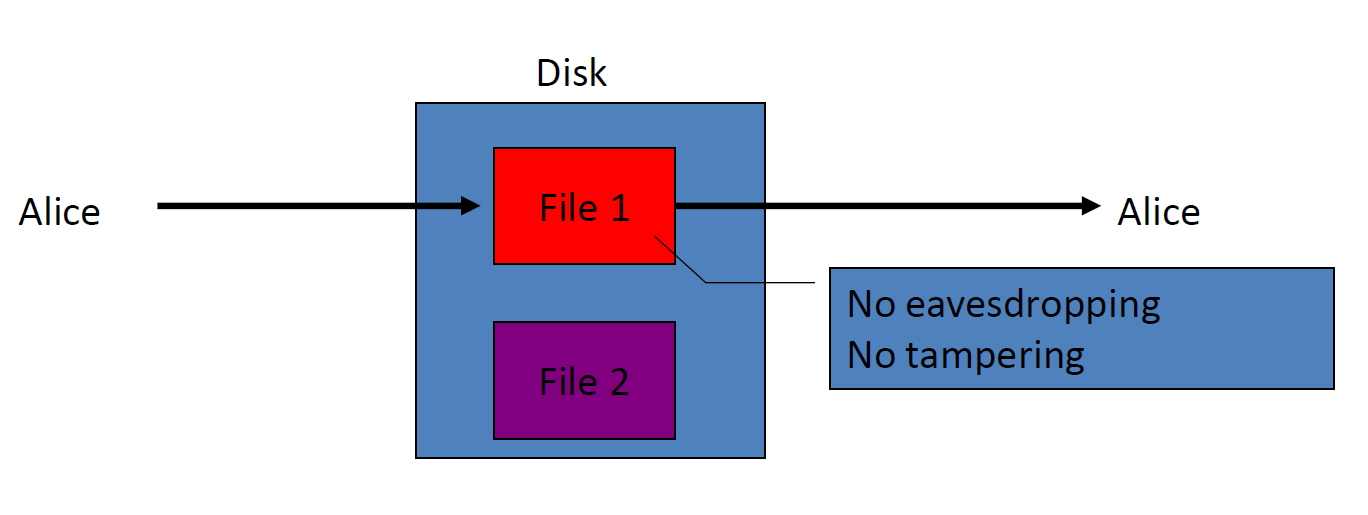
\includegraphics[scale=0.55]{fig1-1.png}\\
%\captionsetup{labelsep=colon}
\caption{}
\end{figure}
\paragraph{} Now, the building block for securing traffic is what's called symmetric encryption systems. And we're going to talk, in the first half of the lecture  extensively about symmetric encryption systems. So, in a symmetric encryption system, basically, the two parties, Alice and Bob, share a secret key k, which the attacker does not know. Only they know the secret key K. Now, they're going to use a cipher which consists of these two algorithms, E and D. E is called an \underline{Encryption algorithm} and D is called the \underline{Decryption algorithm}. The encryption algorithm takes the message and the key as inputs, and produces a corresponding ciphertext. And the decryption algorithm does the opposite. It takes the ciphertext as input along with the key and produces the corresponding message. 

\begin{figure}[H]
\centering
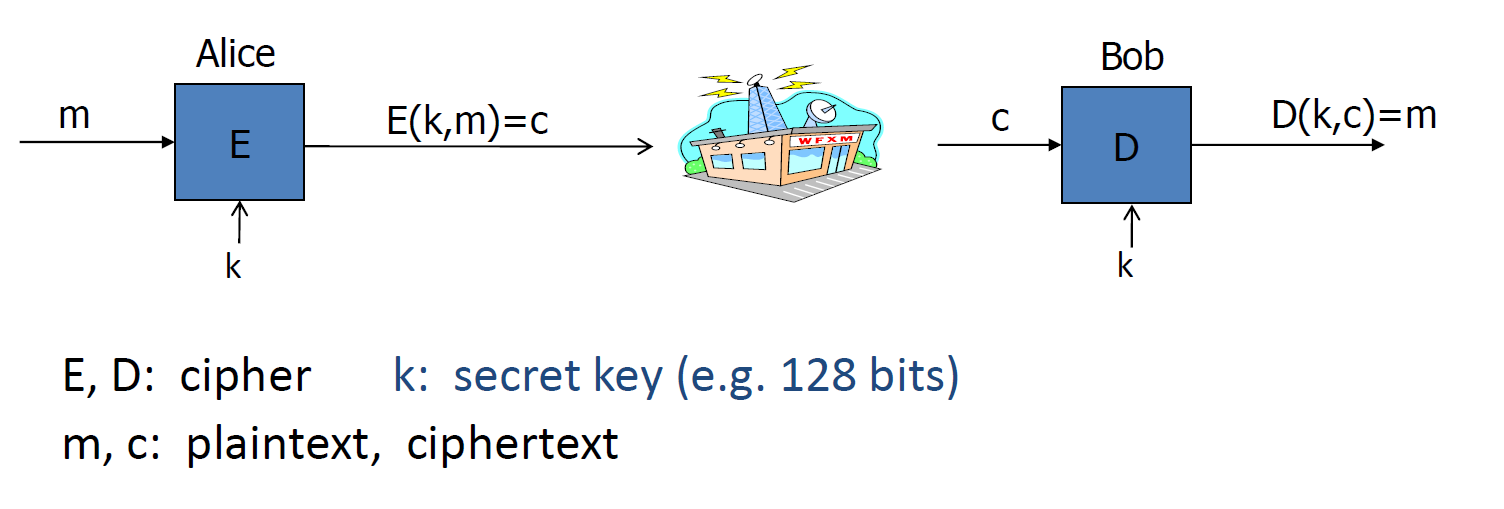
\includegraphics[scale=0.45]{fig1-2.png}\\
%\captionsetup{labelsep=colon}
\caption{}
\end{figure}
\paragraph{}
\begin{note}
I'm only going to say this once now and never again, but it is an extremely important point. And that is: that the algorithms E and D, the actual encryption algorithms are publicly known. Adversary knows exactly how they work. The only thing that's kept secret is the secret key k. Other than that 
everything else is completely public and it's really important to realize that you 
should only use algorithms that are public because those algorithms have been 
peer-reviewed by a very large community of hundreds of people for many, many, many years, 
and these algorithms only begin to be used once this community has shown that 
they cannot be broken, essentially. So, in fact, if somebody comes to you and says, hey, I have a proprietary cipher that you might want to use, the answer usually should be that you stick to standards, to standard algorithms, and not use a proprietary cipher. In fact, there are many examples of proprietary ciphers that, as soon as they were reverse engineered; they were easily broken by simple analysis.
\end{note} 
\paragraph{}Now, even in the simple cases of symmetric encryption which we're going to discuss 
in the first half of the course, there are actually two cases that we're going to discuss in turn. The first, is when every key is only used to encrypt a single message, we call these one-time keys. So, for example, when you encrypt email messages, it's very common that every single email is encrypted using a different symmetric key. Different symmetric cipher key. Because the key is used to encrypt only one message there are actually fairly efficient and simple ways of encrypting messages using these one-time keys and we'll discuss those actually in the next module. Now there are many cases in fact where keys need to be used to encrypt multiple messages. We call these many time keys. For example, when you encrypt files in a file system the same key is used to encrypt many different files. And it turns out if the key is now going to be used to encrypt multiple messages, we need a little bit of more machinery to make sure that the encryption system is secure. In fact, after we talk about the one-time keys, we will move over and talk about encryption modes that are specifically designed for many-time keys. And we'll see that there are a couple more steps that need to be taken to ensure security in those cases. 

\paragraph{}The last point I want to make is that there are a couple of important things to remember about cryptography. First of all, cryptography, of course, is a fantastic tool for protecting information in computer systems. However, it's also very important that cryptography has its limitations. First of all, cryptography is really not the solution to all security problems. For example, if you have software bugs then very often cryptography is not going to be able to help you. Similarly, if you're worried about social engineering attacks, where the attacker tries to fool the user into taking actions that are going to hurt the user, then cryptography is very often actually not going to help you. So, it's very important that although it's a fabulous tool, it's not the solution to all security problems.

\paragraph{}One more very important point is that cryptography essentially becomes useless if it's implemented incorrectly. So, for example, there are a number of systems that work perfectly fine. And we'll see examples of those systems, that, in fact, allow Alice and Bob to communicate. And, in fact, messages that Alice sent to Bob, Bob can receive and decrypt. However, because cryptography is implemented incorrectly, the systems are completely insecure. Actually, I should say that I like to mention an old encryption standard called WEP this is used for encrypting Wi-Fi traffic. WEP contains many mistakes in it and often when I want to show you how not to do things in cryptography, I will point to how things were done in WEP as an example. So, for me, it's very fortunate to have an example, a protocol I can point to for how not to do things.
\paragraph{}And finally, a very important point that I'd like you to remember is that cryptography is not something you should try to invent and design yourself. As I said, there are standards in cryptography, standard cryptographic primitives which we're going to discuss at length during this course. And primarily you're supposed to use these standard cryptographic primitives, and not invent things, these primitives, yourself. The standards have all gone through, many years of review by hundreds of people, and that's not something that's going to happen to an ad hoc design. And, as I said, over the years there are many examples of ad hoc designs that were immediately broken as soon as they were analyzed.
\paragraph{}Before we start with the technical material, I want to give you a quick overview of what cryptography is about and the different areas of cryptography. So, the core of cryptography of course is secure communication that essentially consists of two parts. The first is secured key establishment and then how do we communicate securely once we have a shared key. We already said that secured key establishment essentially amounts to Alice and Bob sending messages to one another such that at the end of this protocol, there's a shared key that they both agree on, shared key K, and beyond that, beyond just a shared key, in fact Alice would know that she's talking to Bob and Bob would know that he's talking to Alice. But a poor attacker who listens in on this conversation has no idea what the shared key is. And we'll see how to do that later on in the course.
\\ 
Once they have a shared key, they want exchange messages securely using this key, and we'll talk about encryption schemes that allow them to do that in such a way that an attacker can't figure out what messages are being sent back and forth. Furthermore, an attacker cannot even tamper with this traffic without being detected. In other words, \underline{these encryption schemes provide both confidentiality and integrity}. 

\paragraph{}But cryptography does much, much more than just these two things. And I want to give you a few examples of that. So, the first example I want to give you is what's called a digital signature. So, a digital signature, basically, is the analog of the signature in the physical world. In the physical world, remember when you sign a document, essentially, you write your signature on that document and your signature is always the same. You always write the same signature on all documents that you want to sign. In the digital world, this can't possibly work because if the attacker just obtained one signed document from me, he can cut and paste my signature unto some other document that I might not have wanted to sign. And so, it's simply not possible in a digital world that my signature is the same for all documents that I want to sign. 
\\
So, we're going to talk about how to construct digital signatures in the second half of the lecture . It's really quite an interesting primitive and we'll see exactly how to do it. Just to give you a hint, the way digital signatures work is basically by making the digital signature via function of the content being signed. So, an attacker who tries to copy my signature from one document to another is not going to succeed because the signature. On the new document is not going to be the proper function of the data in the new document, and as a result, the signature won't verify. And as mentioned, we're going to see exactly how to construct digital signatures later on and then we'll prove that those constructions are secure. 

\paragraph{}Another application of cryptography that I wanted to mention, is \underline{anonymous communication}. So, here, imagine user Alice wants to talk to some chat server, Bob. And, perhaps she wants to talk about a medical condition, and so she wants to do that anonymously, so that the chat server doesn't actually know who she is. Well, there's a standard method, called a mixnet, that allows Alice to communicate over the public internet with Bob through a sequence of proxies such that at the end of the communication Bob has no idea who he just talked to. The way mixnets work is basically as Alice sends her messages to Bob through a sequence of proxies, these messages get encrypted and decrypted appropriately so that Bob has no idea who he talked to and the proxies themselves don't even know that Alice is talking to Bob, or that actually who is talking to whom more generally. 


\paragraph{}One interesting thing about this anonymous communication channel is, this is \textbf{bi-directional}. In other words, even though Bob has no idea who he's talking to, he can still respond to Alice and Alice will get those messages. Once we have anonymous communication, we can build other privacy mechanisms. 

\begin{figure}[H]
\centering
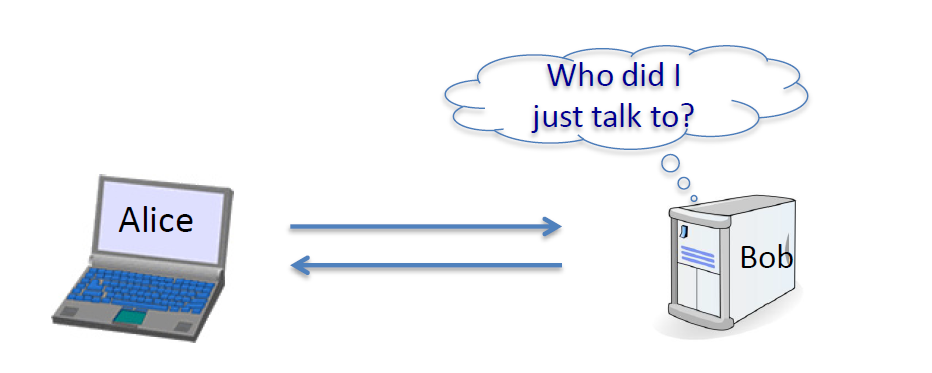
\includegraphics[scale=0.55]{fig1-3.png}\\
%\captionsetup{labelsep=colon}
\caption{}
\end{figure}

\paragraph{}I want to give you one example which is called anonymous digital cash. Remember that in the physical world if I have a physical dollar, I can walk into a bookstore and buy a book and the merchant would have no idea who I am. The question is whether we can do the exact same thing in the digital world. In the digital world, basically, Alice might have a digital dollar, a digital dollar coin. And she might want to spend that digital dollar at some online merchants, perhaps some online bookstore. What we'd like to do is make it so that when Alice spends her coin at the bookstore, the bookstore would have no idea who Alice is. So, we provide the same anonymity that we get from physical cash. The problem is that in the digital world, Alice can take the coin that she had, this one-dollar coin, and before she spent it, she can actually make copies of it. And then all of a sudden instead of just having just one-dollar coin now all of a sudden, she has three-dollar coins and they're all the same of course, and there's nothing preventing her from taking those replicas of a dollar coin and spending it at other merchants.
\paragraph{}
So, the question is how do we provide anonymous digital cash? But at the same time, also prevent Alice from double spending the dollar coin at different merchants. In some sense there's a paradox here where anonymity is in conflict with security because if we have anonymous cash there's nothing to prevent Alice from double spending the coin and because the coin is anonymous, we have no way of telling who committed this fraud. And so, the question is how do we resolve this tension? 
It turns out, it's completely doable. And we'll talk about anonymous digital cash later on. Just to give you a hint, I'll say that the way we do it is basically by making sure that if Alice spends the coin once then no one knows who she is, but if she spends the coin more than once, all of a sudden, her identity is completely exposed and then she could be subject to all sorts of legal problems. That's how anonymous digital cash would work at a high level and we'll see how to implement it later on in the course. 

\paragraph{}
Another application of cryptography has to do with more abstract protocols, but before I speak the general result, I want to give you two examples. So, the first example has to do with election systems. So, here's the election problem:

\paragraph{}Suppose we have two parties, party zero and party one. And voters vote for these 
parties. For example, this voter could have voted for party zero, this voter voted for party one, and so on. So, in this election, party zero got three votes and party two got two votes. The winner of the election, of course, is party zero. But more generally, the winner of the election is the party who receives the majority of the votes. 
\\
Now, the voting problem is the following. The voters would somehow like to compute the majority of the votes, but do it in such a way such that nothing else is revealed about their individual votes. The question is how to do that? And to do so, we're going to introduce an election center who's going to help us compute the majority, but keep the votes otherwise secret. And what the parties will do is they will each send the funny encryption of their votes to the election center in such a way that at the end of the election, the election center is able to compute and output the winner of the election. However, other than the winner of the election, nothing else is revealed about the individual votes. The individual votes otherwise remain completely private.
\\ 
Of course, the election center is also going to verify that this voter for example is allowed to vote and that the voter has only voted once. But other than that information the election center and the rest of the world learned nothing else about that voter's vote other than the result of the election. So, this is an example of a protocol that involves six parties. In this case, there are five voters in one election center. These parties compute amongst themselves. And at the end of the computation, the result of the election is known but nothing else is revealed about the individual inputs. 

\paragraph{}
A similar problem comes up in the context of private auctions. So, in a private auction every bidder has his own bid that he wants to bid. And now suppose the auction mechanism that's being used is what's called a Vickrey auction where the definition of a Vickrey auction is that the winner is the highest bidder. But the amounts that the winner pays is actually the second highest bid. So, he pays the second highest bid.  So this is a standard auction mechanism called the Vickrey auction. 
\paragraph{}
And now what we'd like to do is basically enable the participants to compute, to figure out who the highest bidder is and how much he's supposed to pay, but other than that, all other information about the individual bids should remain secret. So for example, the actual amount that the highest bidder bid should remain secret. The only thing that should become public is the second highest bid and the identity of the highest bidder. So again now, the way we will do that is we'll introduce an auction center, and in a similar way, essentially, everybody will send their encrypted bids to the auction center. The auction center will compute the identity of the winner and in fact he will also compute the second highest bid but other than these two values, nothing else is revealed about the individual bids. 
\paragraph{}
Now, this is actually an example of a much more general problem called \textbf{secure multi-party computation}. Let me explain what secure multi-party computation is about. So here, basically abstractly, the participants have a secret input to themselves. So, in the case of an election, the inputs would be the votes. In the case of an auction, the inputs would be the secret bids. And then 
what they would like to do is compute some sort of a function of their inputs. Again, in the case of an election, the function's a majority. In the case of auction, the function happens to be the second highest, largest number among $X_1$ to $X_4$ . And the question is, how can they do that, such that the value of the function is revealed, but nothing else is revealed about the individual votes? 
\paragraph{}
Let me show you kind of a dumb, insecure way of doing it. What we do is introduce a 
trusted party. And then, this trusted authority basically collects individual inputs. And it kind of promises to keep the individual inputs secret, so that only it would know what they are. And then, it publishes the value of the function, to the world. So, the idea is now that the value of the function became public, but nothing else is revealed about the individual inputs. But, of course, you got this trusted authority that you got to trust, and if for some reason it's not trustworthy, then you have a problem. And so, there's a very central theorem in crypto and it really is quite a surprising fact. That says that any computation you'd like to do, any function F you'd like to compute, that you can 
compute with a trusted authority, you can also do without a trusted authority.
\paragraph{}
 Let me at a high level explain what this means. Basically, what we're going to do, is 
we're going to get rid of the authority. So, the parties are actually not going to send their inputs to the authority. And, in fact, there's no longer going to be an authority in the system. Instead, what the parties are going to do, is they're going to talk to one another using some protocol. Such that at the end of the protocol all of a sudden, the value of the function becomes known to everybody. And yet nothing other than the value of the function is revealed. In other words, the individual inputs are still kept secret. But again, there's no authority, there's just a way for them to talk to one another such that the final output is revealed.

\paragraph{}
 This is a fairly general result, it's kind of a surprising fact that is at all doable. And in fact, it is and towards the end of the class we'll actually see how to make this happen. Now, there are some applications of cryptography that I can't classify any other way other than to say that they are purely magical. 
\paragraph{}
Let me give you two examples of that. So, the first is what's called privately outsourcing computation. I'll give you an example of a Google search just to illustrate the point. So, imagine Alice has a search query that she wants to issue. It turns out that there are very special encryption schemes such that Alice can send an encryption of her query to Google. And then because of the property of the encryption scheme Google can actually compute on the encrypted values without knowing what the plain texts are. So, Google can actually run its massive search algorithm on the encrypted query and recover in encrypted results. Okay. Google will send the encrypted results back to Alice. Alice will decrypt and then she will receive the results. But the magic here is all Google saw was just encryptions of her queries and nothing else. And so, Google as a result has no idea what Alice just 
searched for and nevertheless Alice actually learned exactly what she wanted to learn. So, these are magical kind of encryption schemes. They're fairly recent, this is only a new development from about two or three years ago, that allows us to compute on encrypted data, even though we don't really know what's inside the encryption. 
\paragraph{}
Before you rush off and think about implementing this, I should warn you that this is really at this point just theoretical, in the sense that running a Google search on encryption data probably would take a billion years. But nevertheless, just the fact that this is doable is already really surprising, and is already quite useful for relatively simple computations. So, in fact, we'll see some applications of this later on. 

\begin{figure}[H]
\centering
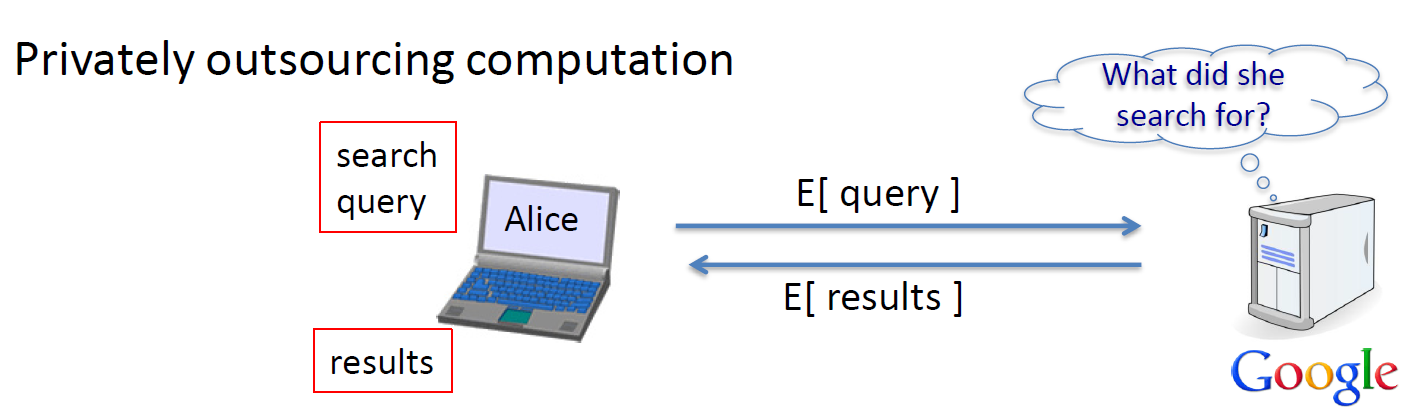
\includegraphics[scale=0.55]{fig1-4.png}\\
%\captionsetup{labelsep=colon}
\caption{}
\end{figure}

\paragraph{}
The other magical application I want to show you is what's called zero knowledge. And in particular, I'll tell you about something called the zero-knowledge proof of knowledge. So here what happens is there's a certain number N, which Alice knows. And the way the number N was constructed is as a product of two large primes. So, imagine here we have two primes, \textbf{p} and \textbf{q}. Each one you can think of it as like 1000 digits. And you probably know that multiplying two 1000-digit numbers is fairly easy. But if I just give you their product, figuring out their factorization into primes is actually quite difficult. In fact, we're going to use the fact that factoring is difficult to build public key cryptosystems in the second half of the course. so Alice happens to have this number N, and she also knows the factorization of N. Now Bob just has the number N. He doesn't actually know the factorization. 
\paragraph{}
Now, the magical fact about the zero-knowledge proof of knowledge, is that Alice can prove to Bob that she knows the factorization of N. You can actually give this proof to Bob, that Bob can check, and become convinced that Alice knows the factorization of N, however Bob learns nothing at all. About the factors \textbf{p} and \textbf{q}, and this is provable. Bob absolutely learns nothing at all about the factors \textbf{p} and \textbf{q}. 
\paragraph{}
And the statement actually is very, very general. This is not just about proving the factorization of N. In fact, almost any puzzle that you want to prove that you know an answer to, you can prove it is your knowledge. So, if you have a crossword puzzle that you've solved. Well, maybe crosswords are not the best example. But if you have like a Sudoku puzzle, for example, that you want to prove that you've solved, you can prove it to Bob in a way that Bob would learn nothing at all about the solution, and yet Bob would be convinced that you really do have a solution to this puzzle. Okay. So those are kind of magical applications. 
\paragraph{}
The last thing I want to say is that modern cryptography is a very rigorous science. And in fact, every concept we're going to describe is going to follow three very rigorous steps, and we're going to see these three steps again and again and again so I want to explain what they are. So, the first thing 
we're going to do when we introduce a new primitive like a digital signature is, we're going to specify precisely what the threat model is. That is, what can an attacker do to attack a digital signature and what is his goal in forging signatures?  So we're going to define exactly what does it mean for a signature for example to be unforgeable. And I'm giving digital 
signatures just as an example. 
\paragraph{}
For every primitive we describe we're going to precisely define what the threat model is. Then we're going to propose a construction and then we're going to give a proof that any attacker that's able to attack the construction under this threat model. That attacker can also be used to solve some underlying hard problem. And as a result, if the problem really is hard, that actually, proves that no attacker can break the construction under the threat model. Okay. But these three steps are actually quite important. In the case of signatures, we'll define what it means for a signature to be, forgeable, then we'll give a construction, and then for example we'll say that anyone who can break our construction can then be used to say factor integers, which is believed to be a 
hard problem. Okay, so we're going to follow these three steps throughout, and then you'll see how this actually comes about.

\begin{note}
The three steps in cryptography: 
\begin{itemize}
\item Precisely specify threat model 
\item Propose a construction 
\item Prove that breaking construction under threat mode will solve an underlying hard problem 
\end{itemize}
\end{note}

\subsection{History of Cryptography}
\paragraph{}
Before we start with the technical material, I want to tell you a little bit about the history of cryptography. There's a beautiful book on this topic by \textbf{David Kahn} called the codebreakers. It covers the history of cryptography all the way from the Babylonian era, to the present. Here, I'm just going to give you a few examples of historical ciphers, all of which are badly broken. 
\paragraph{}
So, to talk about ciphers the first thing I'm going to do is introduce our friends Alice and Bob, who are going to be with us for the rest of the quarter. So, Alice and Bob are trying to communicate securely and there is an attacker who's trying to eavesdrop on their conversation. So, to communicate securely, they're going to share a secret key, which I'll denote by \textbf{K}. They both know the secret key. But the attacker does not know anything about this key K. So now they're going to use a cipher, which is a pair of algorithms, an encryption algorithm denoted by E, and a decryption algorithm, D. 
\paragraph{}
These algorithms work as follows: the encryption algorithm E takes the message M as inputs. And it takes as inputs, the key K. I'm going to put a wedge above the key input just to denote the fact that this input is really the key input. And then it outputs a ciphertext. Which is the encryption of the message M using the key K. I'm always going to write the key first.
$ C := E(K,M) $


 Now, and when I write: = what I mean is that the expression defines what C what the variable C stands for. Now the ciphertext is transmitted over the internet to Bob, somehow. Actually, it could be transmitted over the internet. Could be transmitted using an encrypted file system, it doesn't really matter, but when the ciphertext reaches Bob, he can plug it into the decryption algorithm and give the decryption algorithm the same key K. Again, I'm going to put a wedge here as well. To denote the key inputs and the decryption algorithm outputs the original plaintext message. 
\paragraph{}
The reason we say that these are symmetric ciphers is that both the encrypter and decrypter actually use the same key K. As we'll see later in the course, there are ciphers where the encrypter uses one key and the decrypter uses a different key. But here we're just going to focus on symmetric cipher where both sides use the same key. 
\paragraph{}
So let me give you a few historic examples of ciphers. The first example, the simplest one is called the substitution cipher. I am sure all of you played the substitution ciphers when you were in kindergarten. Basically, a key for a substitution cipher is a substitution table that basically says how to map our letters. So here for example the letter A would be mapped to C, the letter B would be mapped to W the letter C would be mapped to N so on and so forth and then the letter Z would be mapped, say, to A. So, this is one example of a key for a substitution cipher. So just to practice the notation we introduced before, the encryption of a certain message using this key, let's say the message is BCZA, the encryption of this message using this key here would be, is done by substituting one letter at a time. So, B becomes W, C becomes N, Z becomes A, and A becomes C. So, the encryption of BCZA is WNAC, and this defines the ciphertext. Similarly, we can decrypt the ciphertext using the same key and of course we'll get back the original message. 

\begin{figure}[H]
\centering
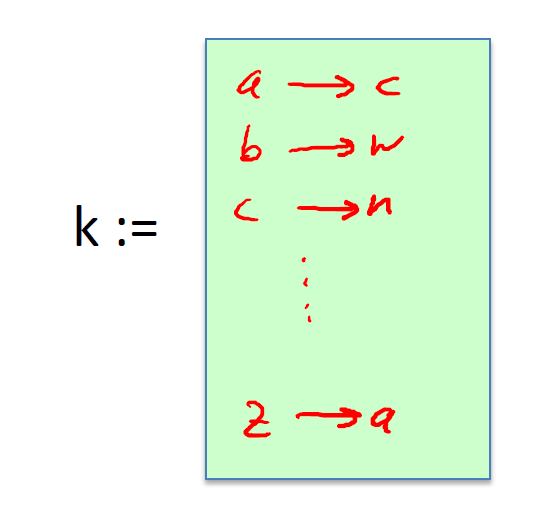
\includegraphics[scale=0.55]{fig1-5.png}\\
%\captionsetup{labelsep=colon}
\caption{}
\end{figure}

\paragraph{}Just for historical reasons, there is one example of something that's related to the substitution cipher called the \underline{Caesar cipher}. The Caesar cipher, actually, is not really a cipher at all. And the reason is that it doesn't have a key. What a Caesar cipher is, is basically a substitution cipher where the substitution is fixed. Namely, it's a shift by three. So, A becomes D, B becomes E, C becomes F and so on and so forth. What it is, Y becomes B and Z becomes C. It's a fixed substitution that's applied to all plaintext messages. So, again, this is not a cipher, because there is no key, the key is fixed. So, if an attacker knows how our encryption scheme works, he can easily decrypt the message. The key is not random, and therefore, decryption is very easy once you understand how the scheme actually works. 
\paragraph{}
So now, let's go back to the substitution cipher, where the keys really are chosen at random, the substitution tables are chosen at random. And let's see how we break this substitution cipher. Turns out to be very easy to break. The first question is, how big is the key space? How many different keys are there, assuming we have 26 letters? The number of keys is 26 factorial, because, a key, a substitution key, is simply a table, a permutation of all 26 letters. The number of permutations of 26 letters, is 26 factorial. If you calculate this out, twenty-sixth factorial is about $2^{88}$, which means that describing a key in a substitution cipher takes about 88 bits. So, each key is represented by about 88 bits. 
\\
Now, this is a perfectly fine size for a key space. In fact, we're going to be seeing ciphers that are perfectly secure, or, you know, that are adequately secure, with key spaces that are roughly of this size. However, even though the substitution cipher has a large key space of size $2^88$, it's still terribly insecure. Let's see how to break it. And to break it, we're going to be using letter frequencies. 
\paragraph{}
The first question is, what is the most frequent letter in English text?  In fact, E is the most common letter. And that is going to, if we make it quantitative, that's going to help us break a substitution cipher. So just given the ciphertext, we can already recover the plaintext. So, the way we do that is, first of all, using frequencies of English letters. 
\paragraph{}
Here's how this works. You give me an encrypted message using the substitution cipher. All I know is that the plaintext is in English and I know that the letter E is the most frequent letter in English. And in fact, it appears 12.7 percent of the time in standard English texts. So, what I'll do is I'll look at the ciphertext you gave me and I'm going to count how many times every letter appears. Now the most common letter in the ciphertext is going to be the encryption of the letter E with very high probability. So now I'm able to recover one entry in the key table. Mainly now I know what the letter E maps to. The next, most common letter in English is the letter T, that appears about 9.1 percent of the time. So now again, I count how many times each letter appears in the ciphertext. And the second most frequent letter is very likely to be the encryption of the letter T. So now I've recovered a second entry in the key table. And I can continue this way. In fact, the letter A is the next most common letter; it appears 8.1 percent of the time. So now I can guess that the third most common letter in the ciphertext is the encryption of the letter A. And now I've recovered three entries in the key table.
\paragraph{}
 Well, so now what do I do? The remaining letters in English appear roughly same amount of time, other than some rare letters like Q and X. But we're kind of stuck at this point. We figured out three entries in the key table but what do we do next? So, the next idea is to use frequencies of pairs of letters. Sometimes these are called digrams. So, what I'll do is, I'll count how many times each pair of letters appears in the ciphertext, and, I know that in English, the most common pairs of letters are things like, HE, AN. IN, I guess TH is another common pair of letters. 
And so, I know that the most common pair of letters in the ciphertext is likely to be the encryption of one of these four pairs. By trial and error, I can sort of figure out more elements in the key table and again by more trial and error this way by looking at trigrams. I can actually figure out the entire key table. 
\paragraph{}
So, the bottom line here is that in fact the substitution cipher is vulnerable to the worst possible type of attack namely a ciphertext only attack. Just given the ciphertext the attack that can recover the decryption key and therefore recover the original plaintext. So, there's really no point in encrypting anything using the substitution cipher, because the attacker can easily decrypt it all; you might as well send your plaintext completely in the clear. 

\begin{figure}[H]
\centering
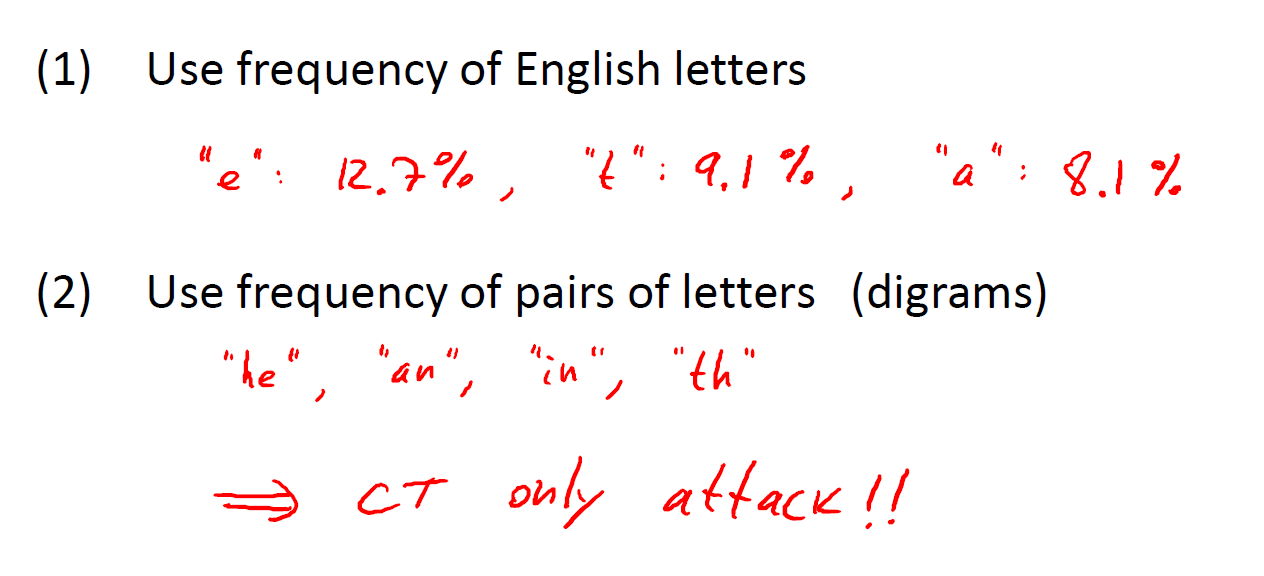
\includegraphics[scale=0.55]{fig1-6.png}\\
%\captionsetup{labelsep=colon}
\caption{}
\end{figure}

\paragraph{}Now we're going to fast-forward to the Renaissance, and, I guess we're moving from the Roman Era to the Renaissance, and look at a cipher designed by a fellow named Vigener, who lived in the sixteenth century. He designed a couple of ciphers. Here I'm going to show you a variant of one of his ciphers, this is called a \textbf{Vigener cipher}. So, in a Vigener cipher, the key is a word. In this case the word, is CRYPTO, it's got six letters in it. And then to encrypt a message, what you do is, you write the message under the key. So, in this case the message is "WHAT A NICE DAY TODAY" and then you replicate the key as many times as needed to cover the message. And then the way you encrypt is basically, you add the key letters to the message letters, modulo 26.
\paragraph{}
 So just to give you an example here, for example, if you add Y and A, you get Z. If you add T and A, you get U. And you do this for all the letters. And remember, whenever you add, you add modulo 26. So, if you go past Z, you go back to A. So, that's the Vigener cipher. And in fact, decryption is just as easy as encryption. Basically, the way you would decrypt is, again, you would write the ciphertext under the key. You would replicate the key and then you would subtract the key from the ciphertext to get the original plain text message.
\begin{figure}[H]
\centering
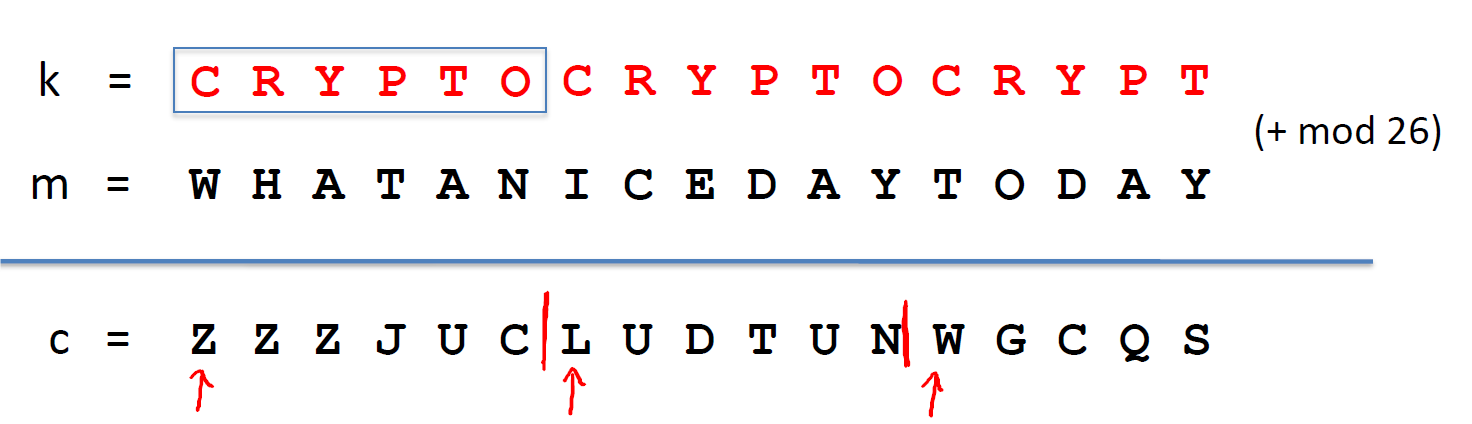
\includegraphics[scale=0.55]{fig1-7.png}\\
%\captionsetup{labelsep=colon}
\caption{}
\end{figure}

\paragraph{}
Breaking the Vigener cipher is actually quite easy. Let me show you how you do it. The first thing we need to do is we need to assume that we know the length of the key. So, let's just assume we know that. In this case, the length of the key is six. And then what we do is we break the cipher text into groups of six letters each, okay? So, we're going to get a bunch of groups like this. Each one, contains six letters. And then we're going to look at, the first letter in each group. In this case, we're looking at the first letter, every six characters. Now, what do we know about these six letters? We know that, in fact, they're all encrypted using the same letter in the ciphertext. All of these are encrypted using the letter C. In other words. Z L W is a shift by three of the plaintext letters. So, if we collect all these letters then the most common letter among the set is likely to be the encryption of E,  E is the most common letter in English, therefore, if I look at every sixth letter, the most common letter in that set is likely to be the encryption of the letter E. 
\paragraph{}

Let's just suppose that in fact the most common letter every sixth letter happens to be the letter H. Then we know that E plus the first letter of the key is equal to H. That says that the first letter of the key is equal to H minus E. And in fact, that is the letter C. So now we've recovered the first letter of the key. 
Now we can continue doing this with the second letter. So, we look at the second letter in every group of six characters and again, we repeat the same exercise. We find the most common letter among the sets and we know that the most, this most common letter is likely the encryption of E and therefore whatever this letter, whatever this most common letter is if we subtract 'E' from it we're going to get the second letter of the key. And so on and so forth. With, the third letter every six characters. And this way we recover, the entire key. And that allows us to decrypt, the message. 
\paragraph{}
Now, the only caveat is that I had to assume ahead of time that I know the length of the key, which in this case is six. But if I don't know the length of the key ahead of time, that's not a problem either. What I would do is I would run this decryption procedure, assuming the key length is one. Then I'd run it assuming the key length is two. Then I would run it assuming the key lengths is three. And so on, and so on, and so on, until finally I get a message. I get a decryption that makes sense. And once I do that, I know that I've kind of recovered the right length of the key and I know that I've also recovered the right key and therefore the right message. 
\paragraph{}
So  very quickly, you can recover, you can decrypt Vigener ciphers. Again, this is a ciphertext only attack. The interesting thing is, Vigener had a good idea here. This addition mod 26 is actually a good idea, and we'll see that later, except it's executed very poorly here. And so we'll correct that, a little bit later. 
\paragraph{}
We're going to fast-forward now from the Renaissance to, to the 19th century where everything became electric. And so people wanted to design ciphers that use electric motors. In particular, these ciphers are called rotor machines because they use rotors. So, an early example is called the \textbf{Hibber machine} which uses a single motor. Here you have a picture of this machine. The secret key is embedded inside of this disc, which rotates by one notch every time you press a key on the typewriter. So, every time you hit a key, the disc rotates by one notch. 
\paragraph{}
Now what does this key do? Well, the key actually encodes a substitution table. And therefore, the disc actually is the secret key. And as I said, this disc encodes a substitution table. In this case, if you happen to press C as the first letter, output would be the letter T. And then the disc would rotate by one notch. After rotating, rotating by one notch, the new substitution table becomes the one shown here. You see that E, basically, moves up, and then the remaining letters move down. Imagine this is basically a two-dimensional rendering of the disc rotating by one notch. Then you press the next letter. And the disc rotates again. You notice again N moved up and the remaining letters moved down. So, in particular, if we hit the letter C three times, the first time we would output, the output would be T, the second time the output would be S, and the third time the output would be K. This is how the single rotor machine works and as it turned out very quickly after it was advertised it was again broken basically using letter frequency, digram frequencies and trigram frequencies. It's 
not that hard given enough ciphertext to directly recover the secret key and then the message. Again, a ciphertext only attack. 

\begin{figure}[H]
\centering
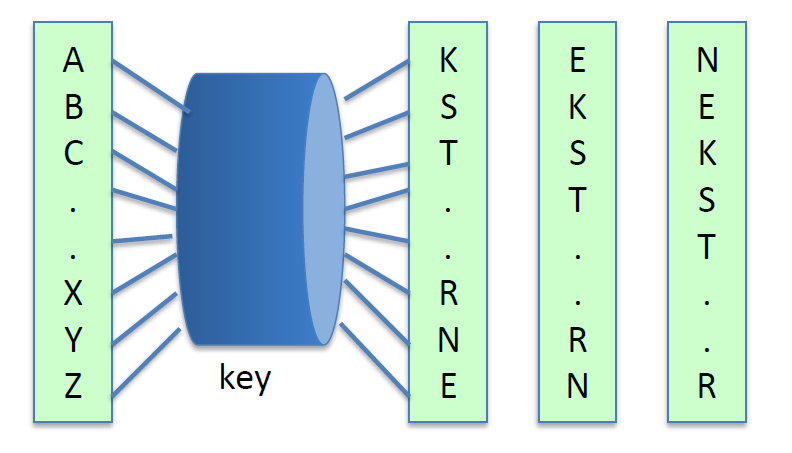
\includegraphics[scale=0.55]{fig1-8.png}\\
%\captionsetup{labelsep=colon}
\caption{}
\end{figure}

\paragraph{}So, to kind of work against these frequency attacks, these statistical attacks, these rotor machines became more and more complicated over time. Until finally, I'm sure you've all heard of the \textit{\textbf{Enigma}}. The Enigma is a kind of complicated rotor machine. It uses three, four, or five rotors. There are different versions of the Enigma machine. Here you see an example of the Enigma machine with three rotors. The secret key in the Enigma machine is the initial setting of the rotors. So, in the case of three rotors there would be 26 cubed possible different keys. When you type on the typewriter basically these rotors here rotate at different rates. This is a diagram of an Enigma machine using four rotors. As you type on the typewriter the rotors rotate and output the appropriate, letters of, the ciphertext. So, in this case the number of keys is 26 to the fourth, which is $2^{18}$, which is relatively a small key space. Today you can kind of, brute-force a search using a computer through $2^{18}$ different keys, very, very quickly. You know, my wristwatch can do it in just a few seconds, I guess. And so, these, this Enigma machine was, already was using relatively small key spaces. But I'm sure you've all heard that the British cryptographers at Bletchley Park were able to mount ciphertext only attacks on the Enigma machine. They were able to decrypt German ciphers back in World War Two. And that played an important role in many different battles during the war. 

\begin{figure}[H]
\centering
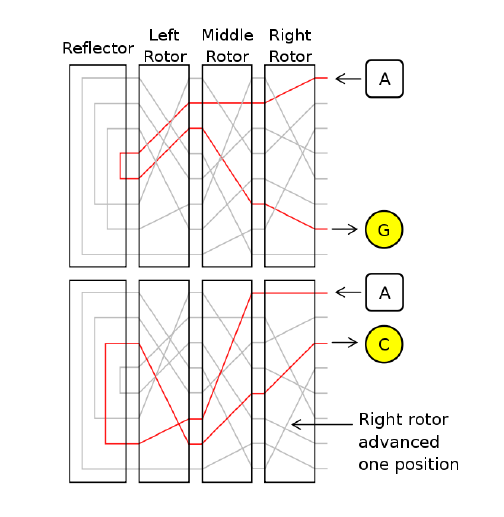
\includegraphics[scale=0.55]{fig1-9.png}\\
%\captionsetup{labelsep=colon}
\caption{}
\end{figure}

\paragraph{}
After the war, I guess that was the end kind of the mechanical age and started the digital age where folks were using computers. And as the world migrated to using computers, the government realized that it's buying a lot of digital equipment from industry. And so, they wanted industry to use a good 
cipher so that when it buys equipment from the, from industry, it would be getting equipment with, with a decent cipher. And so, the government put out this request for proposal for a data encryption standard, a Federal data encryption standard. And we're going to talk about this effort, in more detail later on in the course, but in 1974 a group at IBM put together a cipher that became known as \textbf{\underline{DES}}, \textbf{data encryption standard}, which became a Federal standard for encrypting data. 
\paragraph{}
The key space for DES is $2^{56}$, which is relatively small these days, but was large enough back in 1974. And another interesting thing about DES is, rather than, unlike rotor machines which encrypt one character at a time the data encryption standard encrypts 64 bits at a time, namely eight characters at a time. And we'll see the significance of this later on in the course. 
\paragraph{}
Because DES uses such a small key space, these days it can be broken by a brute-force search and so these days DES is considered insecure and should not be used in projects. Unfortunately, it is used in some legacy systems, but it definitely is on its way out and definitely should not be used in new projects. Today there are new ciphers, things like the advanced encryption standard which uses 128-bit keys. Again, we'll talk about the advanced encryption standards in much more detail later on in the course. There are many, many other types of ciphers. I mentioned Salsa20 here. We'll see why in just a minute. But this is all for the quick historical survey and now we can get into the more technical material.

\section{A crash course on discrete probability}
\subsection{A crash course on discrete probability (Part 1)}

Over the years many natural cryptographic constructions were found to be insecure. In response, modern cryptography was developed as a rigorous science where constructions are always accompanied by a proof of security. The language used to describe security relies on discreet probability. In this segment and the next, I'll give a brief overview of discreet probability, and I point to this Wikibooks article over here for a longer introduction.
\paragraph{}
 Discrete probability is always defined over a universe which I'll denote by U and this universe in our case is always going to be a finite set. In fact, very commonly our universe is going to be simply the set of all n bit strings which here is denoted by (zero , one) to the n.
\paragraph{}
 
For example, the set zero one squared is the set of all two-bit strings which happens to be the string 00011011. There are four elements in this set, and more generally in the set $\left\{0,1\right\}^N$, there are $2^N$ elements. Now a probability distribution over this universe U is simply a function which I'll denote by P, and this function, what it does, is it assigns to every element in the universe a number between zero and one. And this number is what I'll call the weight or the probability of that particular element in the universe. Now there's only one requirement on this function P, and that is that the sum of all the weights, sum up to one. That is, if I sum the probability of all elements X in the universe, what I end up with is the number one.
\paragraph{}

 So, let's look at a very simple example looking back to our 2-bit universe. So, 00011011 And you can consider the following probability distribution Which, for example, assigns to the element 00, the probability $1/2$. The elements 01, we assign the probability 1/8th, to 10 we assign the probability one quarter and to 11 we assign the probability 1/8th. Okay we can see that if we sum up these numbers in fact, we get one which means that this probability P is in fact the probability distribution. Now what these numbers mean is that if I sample from this probability distribution, I'll get the string 00 with probability one half I'll get the string 01 with probability 1/8th and so on and so forth. So now that we understand what a probability distribution is, let's look at two classic examples of probability distributions. The first one is what's called the uniform distribution. 
 \paragraph{}
The uniform distribution assigns to every element in the universe, exactly the same weight. I'm going to use $\left|U\right|$ to denote the size of the universe U. That is the number of elements in the universe, and since we want the sum of all the weights to sum out to one, and we want all these weights to be equal, what this means is that for every element X in the universe, we assign a probability of $P\left(x\right)=\frac{1}{\left|U\right|}$. So, in particular if we look at our example, the uniform distribution and the set of two 8-bit strings, would simply assign one-quarter the weight, $1/4$ to each one of these strings and clearly that, the sum of all the weights sums up to one. Well again, what this means is that if I sample at random from this distribution, I'll get a uniform sample across all our 2-bit strings So all of these 4-bit strings are equally likely to be sampled by this distribution. 

Another distribution that's very common is what's called a point distribution at the point $X_0$ and what this point distribution does is basically it puts all the weight on a single point, namely $X_0$. So here we assign to the point $X_0$ all the weight, one, and then to all other points in the universe, we assign the weight zero.

\begin{equation*}
P(x_0)=1\quad \forall\ x\neq x_0:\,P(x)=0
\end{equation*}

\paragraph{}And by the way, I want to point out that this, $\forall$ here should be read as, for all. So, all this says is, that for all X that are not equal to X zero, the probability of that X is zero. So again, going back to our example a point distribution for example, that would put all its mass on the string 1-0, would assign probability one to the string 1-0 and zero to all other strings. So now if I sample from this distribution pretty much, I'm always guaranteed to always sample the string 1-0 and never sample any of the other strings.
\paragraph{}
 So now we know what a distribution is, and I just want to make one last point, and that is that because this universe U is always going to be a finite set up for us, we can actually write down the weights that the distribution assigns to every element in U, and represent the entire distribution as a vector. So, here for example, if you look at the universe of an all 3-bit strings, we can literally write down the ways that the distribution assigns to the string 000, then the way that distribution assigns to the string 001 And so on, and so forth. We you can see that we can write this as a vector, in this case it will be a vector of dimension eight, there will be, there are eight strings of 3-bits as a result basically the entire distribution is captured by this vector of eight real numbers, in the range of all zero to one.
 \paragraph{} 
The next thing I want to do is define the concept of an \textbf{event}. So, consider a subset A of our universe. And I'll define the probability of the subsets to be simply the sum of the weights of all the elements in the set A. In other words, I'm summing over all X in A, the weights of these elements X in the set A, now because the sum over the entire universe of all weights needs to be one. This means that if we sum, well if you look at the probability of the entire universe, basically we get one. And if we look at the probability of a subset of the universe, we're going to get some number in the interval zero to one and we say that the probability of this set A, is the sum which is a number between zero and one. And I'll tell you that a subset A of the universe is called an event. And the probability of the set A is called the probability of that event. 

\begin{equation*}
A\subseteq U:\quad P\left(A\right)=\sum_{x\in A}P\left(x\right)
\end{equation*}

\paragraph{}
\qs{}{
Let's look at a simple example. So, suppose we look at the universe U, which consists of all 8-bit strings, right? So, the size of this universe U is 256 because there are 256 8-bit strings. Essentially, we're looking at all byte values, all 256 possible byte values. Now let's define the following event. Basically, the event is going to contain all bytes so all 8-bit extremes in the universe such that the two least significant bits of the byte happens to be eleven So for example, if we look at 01011010, that's an element in the universe that's not in the set A. But if we choose a zero to a one, then that's an element of the universe which gives in our set A. And now let's look at the uniform distribution over the universe U and let me ask you what is the probability of the, of the event A? So, what is the probability that when we choose a random byte, the two least significant bits of that byte happens to be 11?} 
\paragraph{}
\sol Well, the answer is one-fourth, and the reason that's true is because it's not too difficult to convince yourself that of the 256 eight-bit strings, exactly 64 of them, one quarter of them, end in one, one. And the probability of each string is, we're looking at the uniform distribution or probability of each string is exactly one over the size of the universe, mainly one over 256. And the product of these, you know, 64 elements, each one has weight one over 256 is exactly one-fourth, which is the probability of the event A that we're looking at.
\paragraph{} 
So, a very simple bound on the probability of events is called the union bound. So, imagine we have two events $A_1$ and $A_2$. So, these are both subsets of some universe U and we want to know what is the probability that either $A_1$ occurs, or $A_2$ occurs in other words, what is the probability of the union of these two events? This little U here denotes the union of the two sets. So, the union bound tells us that the probability that either $A_1$ occurs or $A_2$ occurs is basically less than the sum of the two probabilities. And that's actually quite easy to see. So simply look at this picture here, you can see that when we look at, at the sum of the two probabilities, we're basically summing the probability of all the elements in $A_1$, all the elements in $A_2$ and you realized, we kind of double-summed these elements in the intersection. 

\begin{figure}[H]
\centering
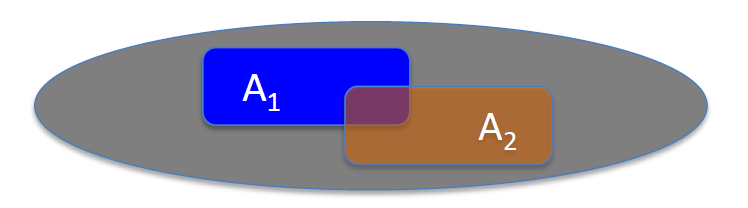
\includegraphics[scale=0.55]{fig1-10.png}\\
%\captionsetup{labelsep=colon}
\caption{}
\end{figure}

\begin{equation*}
P\left(A_1\cup A_2\right)\le P\left(A_1\right)+P\left(A_2\right)
\end{equation*}

\paragraph{}
They get summed twice here on the right-hand side and as a result, the sum of the two probabilities is going to be larger or larger than or equal to, the actual probability of the union of $A_1$ and $A_2$. So that's the classic union bound. And in fact, I'll tell you that if the two events are disjoint, in other words they're intersection is empty, in that case if we look at the sum, at the probability that either $A_1$ or $A_2$ happens, that's exactly equal to the sum of the two probabilities. So, we'll use these facts here and there throughout the lecture. So just to be clear, the inequality holds always but when the two events are disjoint, then in fact we get an equality over here. 
\paragraph{}
So, let's look at another simple example. Suppose our, event $A_1$ is the set of all n-bit stings that happen to end in 1-1 And suppose $A_2$ is the set of all n-bit strings that happen to begin with 1-1. Okay, so N thinks of it as H or some large number and I'm asking that what is the probability that either a one happens or a two happens, in other words if I sample uniformly from the universe U, what is the probability that either the least significant bits are 1-1 or the most significant digits are 1-1. Well as we said that's basically the probability of $A_1\cup A_2$. We know that the probability of each one of these events is one-quarter by what we just did previous slide and therefore by the union bound the probability of the “logical or”. Is, you know, a quarter of the probability of $A_1$, plus the probability of $A_2$, which is a quarter plus a quarter. And we just proved that the probability of seeing 1-1 in the most significant bit, or 1-1 least significant bit, is less than one-half. So that's a simple example of how we might go about using the union bound to bound the probability that one of two events might happen.

\paragraph{}
 The next concept we need to define, is what's called a random variable. Now, random variables are fairly intuitive objects. But unfortunately, the formal definition of a random variable can be a little confusing. So, what I'll do is, I'll give an example, and hopefully that will be clear enough. So formally, a random variable denoted say, by X. Is a function, from the universe into some set V And we say that this set V is where the random variable takes its values. 
 \paragraph{}
So, let's look at a particular example. So, suppose we have a random variable x and this random variable maps into the set 01. So, the values of this random variable are going to be either zero or one. So, one bit, basically. Now, this random variable maps our universe, which is the center of all end bit binary strings, 01 to the end and how does it do it? Well, given a particular sample in the universe, a particular end-bit string y. What the random variable will do is simply output the least significant bit of y and that's it. That's the whole random variable.
\qs{}{  Suppose we look at a uniform distribution on the set $\{0,1\}^N$.  what is the probability that this random variable output zero and what is the probability that a random variable output one?}

\sol Well, you can see that the answers are half and half. Well let's just lead them through why that's the case. So here we have a picture showing the universe and the possible alpha space. And so, in this case the variable can output a zero or a one. When there is a variable output zero, there is a variable output zero when the sample in the universe happens to be, to have its least significant bit be set to zero. In variable one, output one When the sample in the universe happens to have its least significant bit set to one. Well, if choose strings uniformly at random, the probability that we choose a string that has its least significant bits set to zero is exactly $1/2$ Which the random variable output zero with a probability of exactly $1/2$. Similarly, if we choose a random end-bit string, the probability that the least significant bit is equal to one is also $1/2$. And so, we say that the random variable output's one, also with exactly probability of $1/2$. 
\paragraph{}
Now, more generally, if we have a random variable taking values in a certain set V, then this random variable actually induces a distribution on this set V. And here, I just wrote a, kind of a, in symbols, what this distribution means but it's actually very easy to explain. Essentially, what it says is that the variable outputs V Basically, with the same probability that if we sample a random element in the universe, and, and then we apply the function X. We ask, how likely is it that the output is actually equal to V? 
\paragraph{}
So formally we say that the probability that X outputs V, is the same as the probability of the event That when we sample a random element in the universe, we fall into the pre image of V under the function X And again, if this wasn't clear, it's not that important. All you need to know is that a random variable takes values in a particular set V, and in, induces a distribution on that set V.
\paragraph{} 
Now there's a particularly important random variable called a uniform random variable. And it's basically defined as you would expect. So, let's say that U is some finite set for example the set of all N bit binary strings, and we're going to denote a random variable R that's basically sample's uniformly from the set U by this little funny arrow with a little R on top of it. In this, again the notes that the random variable R is literally a uniform random variable sampled over the set U. So, in symbols what's this means is that for all elements A in the universe, the probability that R is equal to A is simply R one over U. And if you want to stick to the formal definition of a, of a uniform variable, it's not actually that important But I would just say that formally the uniform random variable is an identity function namely $r\left(x\right)$ is equal to X for all X in the universe So just to see that this is clear, let me ask you a simple puzzle. 
Suppose we have a uniform random variable over 2-bit strings, so over the set, 01, ten, one and now, let's define a new random variable X to basically sum the first and second bits of R. That is, X simply is the sum of $R_1$ and $R_2$, the first and second bits of R, treating those bits as integers. So, for example, if, R happens to be 00, then X will be 0+0, which is zero. So, let me ask you, what is the probability that X is equal to two? 
It's not difficult to see that the answer is exactly, one-fourth because, basically the only way that X is equal to two is if R happens to be 1,1 but the probability that R is equal to 1,1 is basically one-fourth because R is uniform over the set of all two-bit stings. 
\paragraph{}
The last concept I want to define in this part is what's called a \textbf{randomized algorithm}. These are algorithms that basically take a particular, input data, as input, and they always produce the same output, say Y. So, if we run the algorithm a hundred times on the same input, we'll always get the same output. You can think of a deterministic algorithm as a function that given a particular input data, M, will always produce exactly the same output, A of M. A randomized algorithm is a little different, in that, as before, it takes the input data M as input, but it also has an implicit argument called R, where this R is sampled anew every time the algorithm is run. And in particular this R is sampled uniformly at random from the set of all N-bit strings, for some arbitrary end. Now what happens is every time we run the algorithm on a particular input M, we're going to get a different output because a different R is generated every time. So, the first time we run the algorithm we get one output. The second time we run the algorithm a new R is generated and we get a different output. The third time we run the algorithm a new R is generated and we get a third output and so on. 

\begin{figure}[H]
\centering
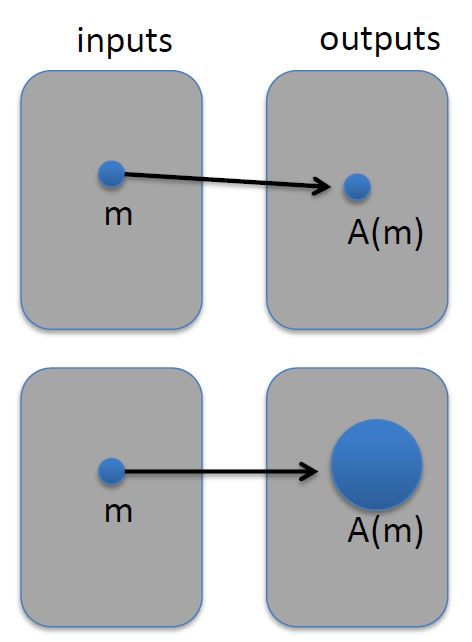
\includegraphics[scale=0.45]{fig1-11.png}\\
%\captionsetup{labelsep=colon}
\caption{}
\end{figure}

\paragraph{}So really the way to think about a randomized algorithm is it's actually defining a random variable.  So given a particular input message, M, it's defining a random variable which is, defining a distribution over the set of all possible outputs of this algorithm, given the input, M. So, the thing to remember is that the output of a randomized algorithm changes every time you run it and in fact, the algorithm defines a distribution and the set of all possible outputs. So, let's look at a particular example.  Suppose we have a randomized algorithm that takes as input a message M And of lecture it also takes an implicate input which is this random string that is used to randomize its operation.  Now what the algorithm will do is simply will encrypt the message M using the random string as input.  this basically defines a random variable. This random variable takes values that are encryptions of the message M And really what this  random variable is it's a distribution over the set of all possible encryptions of the message M under a uniform key.  The main point to remember is that even though the inputs to a randomized algorithm might always be the same every time you run the randomized algorithm; you're going to get a different output. That concludes this segment, and we'll see a bit more discrete probability in the next part.

\subsection{A crash course on discrete probability (Part 2)}
\paragraph{}
In this segment, we're going to continue with a few more tools from discrete probability, and I want to remind everyone that if you want to read more about this, there's more information in wiki books article that is linked over here. So first let's do a quick recap of where we are. We said that the discrete probability is always defined over a finite set, which we're going to denote by U, and typically for us, U is going to be the set of all N bit binary strings, which we denote by $\{0,1\}^N$.
 \paragraph{}
Now a probability distribution P over this universe U is basically a function that assigns to every element in the universe a weight in the interval zero to one, such that if we sum the weight of all these elements, the sum basically sums up to one. Now we have said that subset of the universe is what called an event, and we said that probability of an event is basically the sum of all the weights of all the elements in the event and we said that probability of an event is some real numbers in the interval zero to one and I would remind everyone the basically probability of the entire universe is basically one by the fact that sum of all the weights sums up to one. 
\paragraph{}
Then we define what a random variable is Formally, a random variable is a, is a function from the universe of some other sets but the thing that I want you to remember is that the random variable takes, values in some set v And, in fact, the random variable defines the distribution on this set v. 
\paragraph{}
So, the next concept we need is what's called \textbf{independence} and I'm going to very briefly define this If you want to read more about independence, please go ahead and look at the wiki books article. But essentially, we say that two events A and B are independent of one another if When you know that event A happens, that tells you nothing about whether event B actually happened or not. 
\paragraph{}
\dfn{}{
Formally, the way we define independence is to say that, the probability of A and B, namely, that both events happened, is actually $P\left(A\right)P\left(B\right)$ .}
\paragraph{}
 Multiplication, in some sense, the fact that probabilities multiply under conjunction, captures the fact that these events are independent And as mentioned, if you want to read more about that, please take a look at the background material. 
Now the same thing can be said for random variables. Suppose we have two random variables x and y. They take values in some set v. Then we say that these random variables are independent if the probability that x = a, and y = b is equal to the product of these two probabilities. Basically, what this means is, even if you know that x = a, that tells you nothing about the value of y.  That's what this multiplication means and again this needs to hold for all A and B in the space of values of these random variables 
So, just again to job your memory If you've seen this before, a very quick example. Suppose we look at the, set of, of two-bit strings, $\{00,01,10,11\}$, and suppose we choose a random, from this set. Okay so we randomly choose one of these four elements with equal probability. Now let's define two random variables. x is going to be the least significant bit that was generated, and y is going to be the most significant bit generated. I claim that, these random variables, x and y, are independent of one another. The way to see that intuitively, is to realize that choosing r uniformly, from the set of four elements is basically the same as flipping an unbiased coin twice. The first bit corresponds to the outcome of the first flip and the second bit corresponds to the outcome of the second flip and of course there are four possible outcomes. All four outcomes are equally likely which is why we get the uniform distributions over two-bit strings. 
Now our variables x and y are independent. Basically, if I tell you result of the first flip namely, I tell you the lest signify bit of R So I tell you how the first coin you know whether it fell on its head or fell on its tails. That tells you nothing about the result of the second flip. Which is why intuitively, you might, you might expect these random variables to be independent of one another. But formally, we would have to prove that, for, all 01 pairs, the probability of, $x=0$ and $y=0$, $x=1$, $y=1$, and so on. These probabilities multiply. Let's just do it for one of these pairs. So, let's look at the probability that x=0, and y=0. Well, you see that the probability that $x=0$ and y=0 is basically the probability that r is equal to 00 And what's the probability that r=00?
\paragraph{} 
Well, by the uniform distribution, that's basically equal to $\frac{1}{4} $. It is one over side of the set which is one fourth in this case and well low and behold that's in fact these probabilities multiply because again the probability that X is equal to zero is the probability that lest significant bit of R is equal to zero. This probability is exactly one half because there are exactly two elements that have their, lest signify bit equals to zero. Two out of four elements give you a provability of one half and similarly the probability that Y is equal to zero is also one half so in fact the provability multiplies.
\paragraph{}
 So that's, this concept of independence and the reason I wanted to show you that is because we're going to look at an, an important property of \textbf{XOR} that we're going to use again and again. So, before we talk about XOR, let me just do a very quick review of what XOR is. So, of course, XOR of two bits means the addition of those bits, modular two. So just too kind of, make sure everybody's on the same page If we have two bits, so 00011011. Their XOR or the truth table of the XOR is basically just the addition modular two. As you can see, $1\oplus1=2 \;\mathrm{mod}\,2 $. That's zero. So, this is the truth table for XOR And I'm always going to denote XOR by $\oplus$ and then when I want to apply XOR to bit strings, I apply the addition modular two operation, bitwise. 


\begin{table}[H]
\centering
 \begin{tabular}{||c c c||} 
 \hline
 $x$ & $y$ & $x\oplus y$  \\ [0.5ex] 
 \hline\hline
 0 & 0 & 0 \\ 
 0 & 1 & 1 \\
 1 & 0 & 1 \\
 1 & 1 & 0 \\ [1ex] 
 \hline
 \end{tabular}
\end{table}

\paragraph{}So, for example, the XOR of these two strings would be, 110, and I guess I'll let you fill out the rest of the XORs, just to make sure we're all on the same page. So of course, is comes out to 1101. 

\begin{figure}[H]
\centering
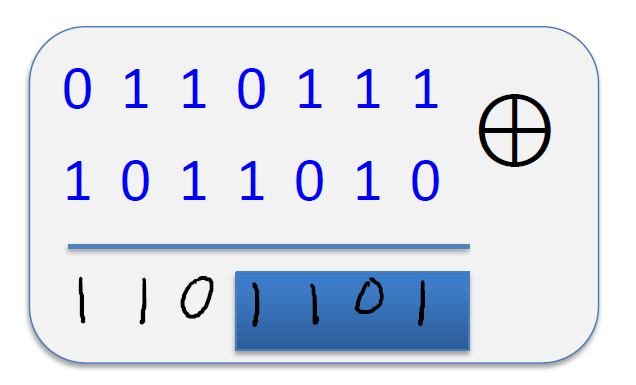
\includegraphics[scale=0.55]{fig1-12.png}\\
%\captionsetup{labelsep=colon}
\caption{}
\end{figure}

\paragraph{}Now, we're going to be doing a lot of XORing in this class. In fact, there's a classical joke that the only think cryptographers know how to do is just XOR things together But I want to explain to you why we see XOR so frequently in cryptography. Basically, XOR has a very important property, and the property is the following. 

\thm{}{If x and y are independent random variables with the uniform distribution on $\{0,1\}^n$ Then $x \oplus y$ is also uniform on $\{0,1\}^n$
}


\paragraph{}Suppose we have a random variable y. That's distributed arbitrarily over 01 to the n. So, we know nothing about the distribution of y but now, suppose we have an independent random variable that happens to be uniformly distributed also over 01 to the n. So, it's very important that x is uniform. N's independent of y. So now let's define the random variable which is the XOR of x and y. Then I claim that no matter what distribution y started with, this z is always going to be a uniform, random variable. So, in other words if I take an arbitrarily malicious distribution and I XOR with independent uniform random variable what I end up with is a uniform random variable. 
\paragraph{}
Okay and this again is kind of a key property that makes x or very useful for crypto. So, this is actually a very simple factor to prove, let's just go ahead and do it, let's just prove it for one bit so for n = one. Okay, so the way we'll do it is we'll basically write out the probability distributions for the various random variables. So, let's see, for the random variable y. Well, the random variable can be either zero or one. And let's say that $P_0$ is the probability that it's equal to zero, and $P_1$ is the probability that it's equal to one. So that's one of our tables. Similarly, we're going to have a table for the variable x. Well, the variable x is much easier. That's a uniform random variable. So, the probability that it's equal to zero is exactly one half the probability that's it's equal to one is also exactly one half. Now, let's write out the probabilities for the join distribution. In other words, let's see what the probability, is for the various, joint values of y and x. In other words, how likely is, it that y=0, and x = 0. Y = 0, and x = 1. Y = 1 and x = 0, and 11.
\paragraph{}
Well, so what we do is, basically, because we assume the variables are independent, all we have to do is multiply the probabilities. So, the probability that y is equal to zero is $p_0$. Probability that x is equal to zero is one-half. So, the probability that, we get 00 as exactly $\frac{p_0}{2}$. Similarly, for 01 we'll get $\frac{p_0}{2}$, for 10 we'll get  $\frac{p_1}{2}$ And for 11, again, the probability that y=1, and x=1, Well, that's $p_1$ the probability that x=1, which is a half, so it's  $\frac{p_1}{2}$. 

\paragraph{}
 So those are the four, probabilities for the various options for x and y. So now, let's analyze, what is the probability that z is equal to zero? Well, the probability that z = 0 is basically the same as the probability that, let's write it this way, xy=00. Or xy=11. Those are the two possible cases that z=0 Because z is the XOR of x and y. Now, these events are disjoint, so, this expression can simply be written as the sum of the two expressions given above. So basically, it's the probability that xy = 00, plus the probability that xy, = 11. So now we can simply look up these probabilities in our table. So the probability that xy = 00 is simply p zero over two, and the probability that xy=11 is simply  $\frac{p_1}{2}$. So, we get  $\frac{p_0}{2} + \frac{p_1}{2}$ But what do we know about $p_0$ and $p_1$? Well, it's a probability distribution. Therefore, $p_0+p_1=1$ and therefore, this fraction here must be equal to a half. $p_0+p_1=1$. So therefore, the sum of these two terms must be a half and we're done. Basically, we proved that the probability that z = 0. Is one half, therefore the probability that z = 1 is also one half. Therefore, z is a uniform random variable. So, the simple theorem is the main reason why XOR is so useful in cartography. 
\paragraph{}
The last thing I want to show you about discrete probability is what's called the \textbf{birthday paradox}. And I'm going to do it really fast here Because we're going to come back later on, and talk about this in more detail. So, the birthday paradox says the following suppose I choose n random variables in our universe U. Okay And it just so happens that these variables are independent of one another. They actually don't have to be uniform. All we need to assume is that they're distributed in the same way. The most important property though is that they're independent of one another. So, the theorem says that if you choose roughly the square root of the size of U elements, we're kind of this one point two here, it doesn't really matter. But if you choose square root of the size of u elements, then basically there's a good chance that there are two elements that are the same. In other words, if you sample about square root a few times, then it's likely that two of your samples will be equal to each other.

\thm{Birthday Paradox}{Let $r_1,\ldots r_n$ be iid random variables in $U$. When $n=1.2\times\sqrt{\left|U\right|}$ we have $
 P(\exists i,j:r_i=r_j)\geq\frac{1}{2}$}

And by the way, I should point out that $\exists$, just means exists. So there exists in U i and j such that $r_i=r_j$. So here's a concrete example. We'll actually see  many times. Suppose our universe consist of all strings of length of 128 bits. So, the size of you is gigantic it's actually 2128. It's a very, very large set but it so happens if you sample say around 264 times from the set. This is about the square root of U then is very likely that two of your sample messages will actually be the same. 
\paragraph{}
So why is, this called the paradox? Well, traditionally it's described in terms of people's birthdays. So, you would think that each of these samples would be someone's birthday and so the question is how many people need to get together so that there are two people that have the same birthday? So, just as a simple calculation you can see there are 365 days in the year, so you would need about 1.2 times the square root of 365 people until the probability that two of them have the same birthday is more than a half. This if I'm not mistaken is about 24, which means that if 24 random people get together in a room it's very likely that two of them will actually have the same birthday. This is why it's called a paradox, because 24 supposedly is a smaller number than you would expect. 
\paragraph{}
Interestingly, people's birthdays are not actually uniform across all 365 days of the year. There's actually a bias towards December. But I guess that's not, that's not relative to the discussion here. The last thing I wanted to do is just show you the birthday paradox a bit more concretely. So, suppose we have a universe of about a million samples, then you can see that when we sample roughly 1200 times, the probability that we get, we sample the same number, the same element twice is roughly half, but the probability of sampling the same number twice actually converges very quickly to one. You can see that if we about 2200 items, then the probability that two of those items are the same, already is 90 percent and You know, 3000 then it's basically one. So, this conversion is very quickly to one as soon as he goes beyond the square root of the size of the universe. So, we're going to come back and study the birthday paradox in more detail later on, but I just for now, wanted you to know what it is. So that's the end of this part, and then in the next part we'll start with our first example of encryption systems.

\begin{figure}[H]
\centering
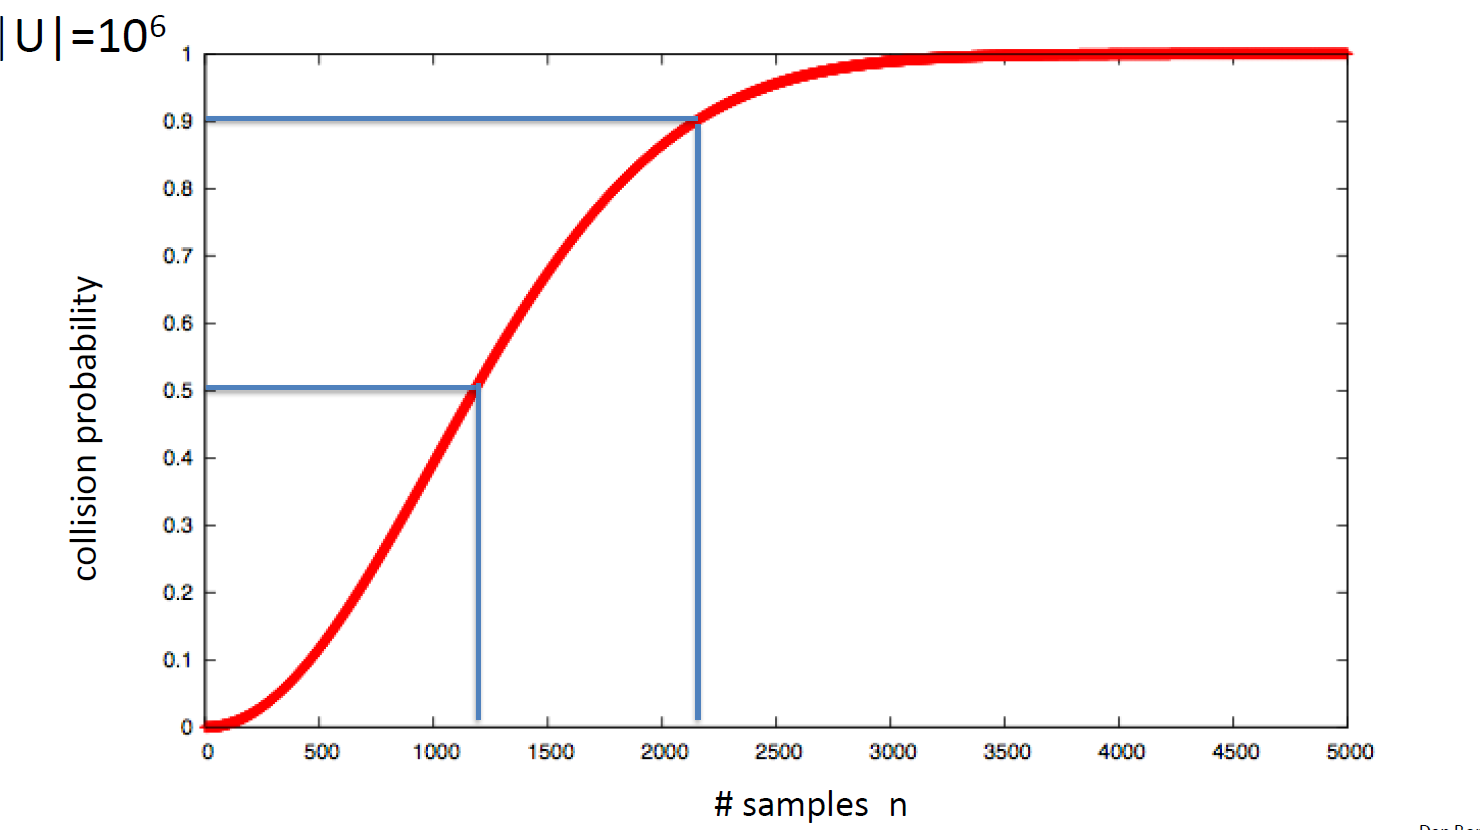
\includegraphics[scale=0.45]{fig1-13.png}\\
%\captionsetup{labelsep=colon}
\caption{}
\end{figure}

\section{Stream Ciphers 1}
\subsection{Information Theoretic Security and The One Time Pad}
\paragraph{}
Now that we've seen a few examples of historic ciphers, all of which are badly broken, we're going to switch gears and talk about ciphers that are much better designed. But before we do that, I want to, first of all, define more precisely what a cipher is. So, first of all, a cipher is actually, remember a cipher is made up of two algorithms. There's an encryption algorithm and a decryption algorithm. But in fact, a cipher is defined over a triple. So, the set of all possible keys, which I'm going to denote by script K, and sometimes I'll call this the key space, it's the set of all possible keys. There's this set of all possible messages and this set of all possible ciphertexts.
\paragraph{} 
So this triple in some sense defines the environment over which the cipher is defined. And then the cipher itself is a pair of efficient algorithms E and D. E is the Encryption algorithm; D is the decryption algorithm. Of course, E takes keys and messages. And outputs ciphertexts. And the Decryption algorithm takes keys and ciphertexts. Then outputs messages. And the only requirements are that these algorithms are consistent. They satisfy what's called the correctness property. So, for every message in the message space. And every key. In the key space, it had better be the case that if I encrypt the message with the key K and then I decrypt using the same key K I had better get back the original message that I started with.

\paragraph{}
 So, this equation here is what's called the consistency equation and every cipher has to satisfy it in order to be a cipher otherwise it's not possible to decrypt. One thing I wanted to point out is that I put the word efficient here in quotes. And the reason I do that is because efficient means different things to different people. If you're more inclined towards theory, efficient means runs in polynomial time. So, algorithms E and D have to run in polynomial time in the size of their inputs. If you're more practically inclined, efficient means runs within a certain time period. So, for example, algorithm E might be required to take under a minute to encrypt a gigabyte of data. Now either way, the word efficient kind of captures both notions and you can interpret it in your head whichever way you'd like. I'm just going to keep referring to it as efficient and put quotes in it as I said if you're theory inclined think of it as polynomial time, otherwise think of it as concrete time constraints.
 \paragraph{}
 Another comment I want to make is in fact algorithm E. It's often a randomized algorithm. What that means is that as your encrypting messages, algorithm E is going to generate random bits for itself, and it's going to use those random bits to actually encrypt the messages that are given to it. On the other hand, the decrypting algorithm is always deterministic. In other words, given the key and the ciphertext output is always the same. Doesn't depend on any randomness that's used by the algorithm.
 \paragraph{}
 So now that we understand what a cipher is better, I want to kind of show you the first example of a secure cipher. It's called a one-time pad. It was designed by Vernam back at the beginning of the twentieth century. Before I actually explain what the cipher is, let's just state it in the terminology that we've just seen. 
So, the message space for the Vernam cipher for the one-time pad is the same as the ciphertext space which is just the set of all ended binary strings. This, this just means all sequences of bits, of zero one characters. The key space is basically the same as the message space which is again simply the embed of all binary strings. So, a key in the one-time pad is simply a random big string, it's a random sequence of bits. That's as long as the message to be encrypted, as long as the message. 
\paragraph{}
Now that we've specified kind of what's the cipher's defined over, we can actually specify how the cipher works and it's actually really simple. So essentially the ciphertexts. Which is the result of encrypting a message with a particular key, is simply the XOR of the two. Simply $K \oplus M$. To see a quick example of this. Remember that XOR, $\oplus$ means addition modulo two. 
So, if I take a particular message, say, 0110111. And it takes a particular key, say 1011001. When I compute the encryption of the message using this key, all I do is I compute the XOR of these two strings. In other words, I do addition module or two bit by bit. So, I get 1101110. That's a ciphertext. And then how do I decrypt? I guess they could do kind of the same thing. So, they decrypt a cipher text using a particular key. What I do is I XOR the key and the ciphertext again. And so, all we have to verify is that it satisfies the consistency requirements. And I'm going to do this slowly once and then from now on I'm going to assume this is all, simple to you. 
\begin{figure}[H]
\centering
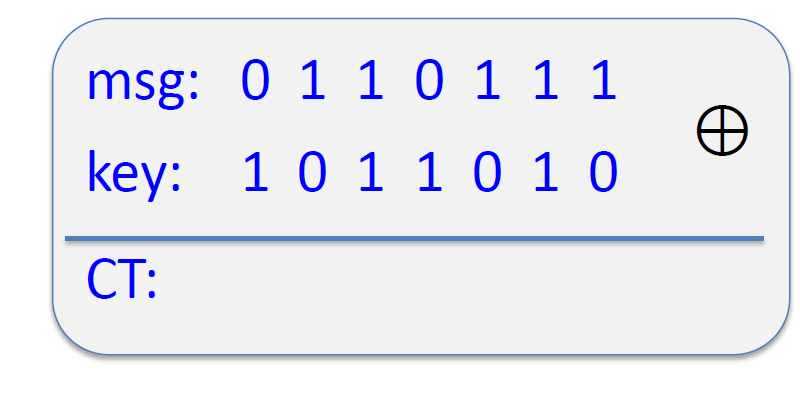
\includegraphics[scale=0.45]{fig1-14.png}\\
%\captionsetup{labelsep=colon}
\caption{}
\end{figure}
 \paragraph{}
So, we're going to make, we're going to have to make sure that if I decrypt a cipher text, that was encrypted using a particular key, I had better get. Back the message M. So, what happens here? Well, let's see. So, if I look at the encryption of k and m, this is just k XOR m by definition. What's the decryption of k XOR m using k? That's just $k \oplus (k\ oplus m)$. And so, since I said that XOR is addition modulo two, addition is associative, so this is the same as $(k \oplus k)\oplus m$, which is simply as you know $k oplus k =0$, and $0\oplus m=m$. 
\paragraph{}
So this actually shows that the one-time pad is in fact a cipher, but it doesn't say anything about the security of the cipher. And we'll talk about security of the cipher in just a minute. First of all, let me quickly ask you a question, just to make sure we're all-in sync. Suppose you are given a message M and the encryption of that message using the one-time pad. So, all you're given is the message and the cipher text. My question to you is, given this pair M and C, can you actually figure out the one-time pad key that was used in the creation of C from M? 
\paragraph{}
So, it's now crystal clear that given the message in the cipher text it's very easy to recover what the key is. In particular the key is simply $M \oplus C$. Then we'll see that if it's not immediately obvious to you we'll see why that's, the case, a little later in the talk, in the lecture.Alright so the one-time pad is a really cool from a performance point of view all you're doing is you XORing the key in the message so it's a super, super fast cipher for encrypting and decrypting very long messages. Unfortunately, it's very difficult to use in practice. The reason it's difficult to use is the keys are essentially as long as the message. So, if Alice and Bob want to communicate securely, so you know Alice wants to send a message end to Bob, before she begins even sending the first bit of the message, she has to transmit a key to Bob that's as long as that message. Well, if she has a way to transmit a secure key to Bob that's as long as the message, she might as well use that same mechanism to also transmit the message itself. 
\paragraph{}
So, the fact that the key is as long as the message is quite problematic and makes the one-time pad very difficult to use in practice. Although we'll see that the idea behind the one-time pad is actually quite useful and we'll see that a little bit later. But for now, I want to focus a little bit on security. So, the obvious questions are, you know, why is the one-time pad secure? Why is it a good cipher? 
\paragraph{}
Then to answer that question, the first thing we have to answer is, what is a secure cipher to begin with? What is a, what makes cipher secure? So the study, security of ciphers, we have to talk a little bit about information theory. And in fact, the first person, to study security of ciphers rigorously. Is very famous, you know, the father of information theory, \textbf{Claude Shannon}, and he published a famous paper back in 1949 where he analyzes the security of the one-time pad. So, the idea behind Shannon's definition of security is the following.
\paragraph{} 
Basically, if all you get to see is the cipher text, then you should learn absolutely nothing about the plain text. In other words, the cipher text should reveal no information about the plain text. And you see why it took someone who invented information theory to come up with this notion because you have to formulize, formally explain what does information about the plain text actually mean. So that's what Shannon did and so let me show you Shannon's definition, I'll write it out slowly first. 
\paragraph{}
So, what Shannon said is you know suppose we have a cipher E D that's defined over triple K M and C just as before. So, K, M and C define the key space, the message space and the cipher text space. And when  we say that the cipher has perfect secrecy if the following condition holds. It so happens for every two messages $m_0$ and $m_1$ in the message space. For every two messages the only requirement I'm going to put on these messages is they have the same length. So, we're only, we'll see why this requirement is necessary in just a minute. And for every ciphertext, in the ciphertext space.
\paragraph{} 
So, for every pair of method message and for every cipher text, it had better be the case that, if I ask, what is the probability that, encrypting $m_0$ with K gives C, okay? So how likely is it, if we pick a random key? How likely is it that when we encrypt $m_0$, we get C. That probability should be the same as when we encrypt $m_1$. Okay, so the probability of encrypting $m_1$ and getting c is exactly the same as the probability of encrypting n zero and getting c. And just as I said where the key, the distribution, is over the distribution on the key. So, the key is uniform in the key space. So, k is uniform in k. And I'm often going to write k arrow with a little r above it to denote the fact that k is a random variable that's uniformly sampled in the key space k. 
\dfn{Perfect Secrecy}{ Let $\mathcal{E} = (E;D)$ be a Shannon cipher defined over $(\mathcal{K};\mathcal{M}; \mathcal{C})$.
Consider a probabilistic experiment in which the random variable k is uniformly distributed over K.
If for all $m_0;m_1 \in \mathcal{M}$, and all $c \in \mathcal{C}$, we have
\[Pr[E(k;m_0) = c] = Pr[E(k;m_1) = c]\];
then we say that $\mathcal{E}$ is a perfectly secure Shannon cipher.
}
\paragraph{}This is the main part of Shannon's definition. And let's think a little bit about what this definition actually says. So, what does it mean that these two probabilities are the same? Well, what it says is that if I'm an attacker and I intercept a particular cipher text C, then in reality, the probability that the cipher text is the encryption of n zero is exactly the same as the probability that it's the encryption of $m_1$. Because those probabilities are equal. So, if I have, all I have the cipher text C that's all I have intercepted I have no idea whether the cipher text came from $m_0$ or the cipher text came from $m_1$ because again the probability of getting C is equally likely whether $m_0$ is being encrypted or $m_1$ is being encrypted. So here, we have the definition stated again. And I just want to write these properties again more precisely. So, let's write this again. So, what this definition means is that if I am given a particular cipher text, I can't tell where it came from. I can't tell if it's, if the message that was encrypted. Is either $m_0$ or $m_1$ and in fact, this property is true for all messages. For all these $m_0$, for all $m_0$ and $m_1$. So not only can I not tell if' C' came from $m_0$ or $m_1$, I can't tell if it came from $m_2$ or $m_3$ or $m_4$ or $m_5$ because all of them are equally likely to produce the cipher text C'.
\paragraph{} 
So, what this means really is that if you're encrypting messages with a one-time pad then in fact the most powerful adversary, I don't really care how smart you are, the most powerful adversary. Can learn nothing about the plain text, from the cipher text. So, to say it in one more way, basically what this proves is that there's no cipher text-only attack on a cipher that has perfect secrecy. 
Now, cipher attacks actually aren't the only attacks possible. And in fact, other attacks may be possible, other attacks may be possible.
\paragraph{}
Now that we understand what perfect secrecy, means, the question is, can we build ciphers that actually have perfect secrecy? And it turns out that we don't have to look very far, the one-time pattern fact has perfect secrecy. So, I want to prove to you this is Shannon's first results and I want to prove this fact to you, it's very simple proof so let's go ahead and look at it and just do it. So, we need to kind of interpret what does that mean, what is this probability that $E(k, m)=c$. So, it's actually not that hard to see that for every message and every ciphertext the probability that the encryption of M under a key K the probability that, that's equal to C, the probability that our random choice of key by definition. All that is basically the number of keys. Such that, well. If I encrypt. And with K I get C. So, I literally count the number of keys and I divide by the total number of keys. Right? That's what it means, that if I choose a random key, that key maps M to C. Right. So, it's basically the number of key that map n to c divided by the total number of keys. This is its probability.
\paragraph{}
 So now suppose that we had a cipher such that for all messages and all cipher texts, it so happens that if I look at this number, the number of  k, such that e, k, m is equal to c. In other words, I'm looking at the number of keys that map m to c. Suppose this number happens to be a constant. So, say it happens to be two, three, or ten or fifteen. It just hap, happens to be an absolute constant. If that's the case, then by definition, $\forall k,m,c$, this probability has to be the same because the denominator is the same, the numerator is the same, it's just as constant, and therefore the probability is always the same for all m and c. And so, if this property is true, then the cipher has perfect secrecy.
 \paragraph{} 
So let’s see what can we say about this quantity for the one-time pad. So, the question to you is, if I have a message in a cipher-text, how many one-time pad keys are there that map, this message M, so the cipher C? So, in other words, how many keys are there, such that $M \oplus K$ is equal to $C$? 
So, I hope you've all answered one. And let's see why that's the case. For the one-time pad, if we have that, the encryption of K of M under K is equal to C. But basically, well, by definition, that implies that K XOR M is equal to C. But that also simply says that $k=m\oplus c$. 
\paragraph{}
 I just $\oplus$both sides by M and I get that $k=m\oplus c$.  So, what that says is that, for the one-time pad, in fact, the number of keys, in K, shows the $E(k,\ m)=c$. That simply is one, and this holds for all messages in cipher text. And so, again, by what we said before, it just says that the one-time pad has, perfect secrecy and that completes the proof of this very, very simple lemma.
\paragraph{}
 Now the funny thing is that even though this lemma is so simple to prove in fact it proves a pretty powerful statement again. This basically says for the one-time pad there is no cipher text only attack. So, unlike the substitution cipher, or the vigenere cipher, or the roller machines, all those could be broken by ciphertext-only attack. We've just proved that for the one-time pad, that's simply impossible. Given the ciphertext, you simply learn nothing about the plaintext. 
 \paragraph{}
However, as we can see, this is simply not the end of the story. I mean, are we done? I mean, basically, we're done with the course now, because we have a way to encrypt, so that an attacker can't recover anything about our method. So maybe we're done with the course. But in fact, as we'll see, there are other attacks. And, in fact, the one time pad is actually not such a secure cipher. And in fact, there are other attacks that are possible, and we'll see that shortly. I emphasize again the fact that it has perfect secrecy does not mean that the one-time pad is the secure cipher to use. 
\paragraph{}
But as we said the problem with the one-time pad is that the secret key is really long. If you had a way of. Communicating the secret key over to the other side. You might as well use that exact same method to also communicate the message to the other side, in which case you wouldn't need a cipher to begin with. So, the problem again is the one-time pad had really long keys and so the obvious question is are their other ciphers that has perfect secrecy and possibly have much shorter keys? 

\thm{}{Perfect secrecy requires $|K|\geq |M|$ (key space size must at least be equal to the message space size, which means key length must be at least equal to the message length)}

\paragraph{}Well, so the bad news is the Shannon, after proving that the one-time pad has perfect secrecy, proved another theorem that says that in fact if a cipher has perfect secrecy, the number of keys in the cipher must be at least the number of messages that the cipher can handle.  So in particular, what this means is if I have perfect secrecy then necessarily the number of keys, or rather the length of my key, must be greater than the length of the message. 
\paragraph{}
So, in fact, since the one-time pad satisfies us with equality, the one-time pad is an optimal, cipher that has perfect secrecy. So basically, what this shows is that this is an interesting notion. The one-time pad is an interesting cipher. But, in fact, in reality, it's actually quite hard to use. It's hard to use in practice, again, because of these long keys. And so, this notion of perfect secrecy, even though it's quite interesting, basically says that it doesn't really tell us the practical ciphers are going to be secure. And we're going to see, but, as we said, the idea behind the one-time pad is quite good. And we're going to see, in the next lecture, how to make that into a practical system.

\subsection{Stream Ciphers and Pseudo Random Generators}

\paragraph{}
Now that we know about the one-time pad, let's talk about making the one-time pad more practical using something called the stream cipher. But before we do that, let's do a quick review of where we were. So, let me just remind you that a cipher is defined over a triple of sets called a key space, a message space, and a cipher text bare space. And a cipher is a pair of efficient algorithms called E and D; E stands for encryption and D stands for decryption. And the only property. That we need to satisfy is that decryption is the opposite of encryption. In other words, if I encrypt a message M using a particular key. And I decrypt using the same key. I get back the original message.
\paragraph{}
 Last time we looked at a couple of weak ciphers like the substitution cipher and the vigonaire cipher. We showed that all of them can be easily broken so you should never ever, ever use those ciphers. Those were just for historical reference. And then we looked at our first example of a good cipher, namely the one-time pad. So, let me just remind you how the one-time pad is defined. Basically, the message space is the set of all bit end bit strings. The cipher text is a set of all bit end bit strings. And similarly, the key. Is the set of all N bit strings and the way we encrypt is by a simple XOR to encrypt the message we just XOR the message in the key that gives us the cipher text. And then to decrypt a cipher text, we just do this $\oplus$ again and it's easier to show by properties of X over that in fact decryption is the opposite of encryption.
 \paragraph{} 
Then we talked about this lemma, in fact, we proved it, that says that the one-time pad has perfect secrecy, which means that if you're just an eavesdropper and you just get to see a single cipher text, you're not going to be able to deduce any information about the encrypted plain text. Unfortunately. We also said that Shannon proved this lemma, we called it the bad news lemma, that basically says that any cipher that has perfect secrecy must have really long keys. In other words, the key length must be at least as long as the length of the message, which means that the cipher is not particularly useful. Because if two parties have a way to agree on really long keys that are as long as the message, they, in some sense, might as well use that mechanism to already transmit the message itself.
 So, in this lecture we're going to take the idea of the one-time pad and try to make it into a practical encryption scheme. So, this is called what's called a stream cipher. So, the idea in this stream cipher is rather than using a totally random key, we're actually going to use a \textbf{Pseudo-Random} key. And to explain how that works, I need to define what is a pseudo-random generator, \textbf{\underline{PRG}}. So, a \textbf{PRG}, really, all it  is just a function, I'll call it g for generator, that takes a seed, so I'm going to use $ \{0,1\}^s$ to denote all strings of length s, so this we'll call the seed space. So, he takes an s bit seed and maps it to a much larger string which will denote by $\{0,1\}^n$. And the property is that $s\ll n$. So, in other words, we take a seed that might be only 128 bits and we expand it into a much, much larger output string that could be gigabytes long. That's what this \textbf{pseudo-random generator} does.
 \paragraph{}
  And of course, the goal is that first of all, the generator is efficiently computable, so the function G. There should be some sort of an efficient algorithm that computes it. So, efficiently computable by a deterministic algorithm. It's important to understand that the function G itself has no more randomness, in it, it's a totally deterministic. The only thing that's random here is the random seed, that's given as input to the function G. And the other property, of course, is that the output. Should look random and the question is what does it mean to look random, and that's something we'll define later on in the lecture.
  \paragraph{}
 So suppose we have such a generator, how do we use that, to build a stream cipher? We the idea is that we're going to use the seed, as our key, so our short seed is going to be our secret key. And then we're going to use the generator to basically expand the seed into a  much larger random looking sequence, or pseudo random sequence, as it's known, so this would be G of K. And then we are going to X over it just like in the one time pad we're going to X over it the student random sequence with the message and that's going to give us the cipher text. Or if we want to write this in math, we'll write C = E(m,k), which is simply defined as $M\oplus G(k)$. And then when we want to decrypt, basically we do exactly the same thing. It's basically the $C\oplus G(k)$, just like in the one-time pad except then instead of XORing with K, we XOR with the output of the generator applied to K.
 \paragraph{} 
So, the first question to ask is why is it secure? So, basically you now, we only have one notion of security so far, which we called perfect secrecy. And so, let's just quickly ask can a stream cipher have perfect secrecy. Remember in the stream cipher the key is  much shorter than the message. And so, nevertheless, can it have perfect secrecy?
So, I hope everybody said the answer is, no. The key is much shorter than the message. And we said that in a, in a perfectly secure cipher, the key must be as long as the message. And therefore, it's not possible that a, that a stream cipher actually has perfect secrecy. So, the question is, then, well, why is it secure? First of all, we would need a different definition of security to argue that Stream Cipher is secure and in particular, the security property is going to depend on the specific generator that we used.
\paragraph{} 
So, in fact the definition of privacy that we'll need to argue the security of Stream Cipher is we'll see in the next lecture, but for now let me show you one particular property. That a generator must have a minimum property needed for security. This property is called \textbf{unpredictability}. So, let's we suppose for one second that in fact a stream cycle is predictable. So, what does that mean? Both the \textbf{PRG} is predictable. What that means is essentially that there is some pi. Such that if I give you the first I bits of the outputs. There is some sort of an algorithm, there's an efficient algorithm that will compute the rest of the string. So given the first I bits, you can compute the remainder of the bits. I claim that if this is the case, then the stream cipher would not be secure. 
\paragraph{}
So, let's see why. Suppose an attacker actually intercepts a particular cipher text, let's call it C. If this is the case, then in fact, we have a problem. Because suppose that just by some prior knowledge, the attacker actually knows that the initial part of the message happens to be some known value. For example, we know that in the mail protocol, \textbf{smtp}, the standard mail call used in the internet, you know that every message starts with a word from colon. Well, that would be a prefix that the adversary knows. That the site, that the message must begin with from a colon. What it could do is it could XOR the cipher text with the words from colon, with the little prefix of the message that it actually knows. And what that would give it is a prefix of the pseudo random sequence. And I would learn as a result of this, it would learn a prefix of the pseudo random sequence but then we know that once it has a prefix of the pseudo random sequence it can predict the remainder of the pseudo random sequence and that would allow it to then predict the rest of the message end. So for example if the pseudo random generator was predictable given five bits of the pad. Then every email encrypted using the stream cipher would be decryptable because, again, the attacker knows the prefix of the message from which he deduces the prefix of the pad, which then allows him to compute the rest of the pad, which then allows him to recover the entire plain text. So this is an example that shows that in fact if a \textbf{PRG} is predictable then already there are security problems. Because a small prefix would reveal the entire message. As it turns out, even if I could predict just one bit of the outputs. 
\paragraph{}
Even if given, you know, the first I bits, I can predict the next bits, the I plus first bits. Already, this is a problem. Because that would say that given again, the first couple of letters in a message can predict, can decrypt essentially, and recover the next bit of the message, or the next layer of the message, and so on. So, this predictability property shows that, you know, if we use a \textbf{PRG} that's going to be used in a stream cipher, it had better be unpredictable.
\paragraph{} 
So, what does it mean that a \textbf{PRG} is unpredictable? So, let's define more precisely what it means for a \textbf{PRG} to be unpredictable. Well first we'll define more precisely what it means for a \textbf{PRG} to be predictable.
\paragraph{}
 Therefor , we say that G is predictable, if there exists an efficient algorithm. Let's call it A and there is some position. There's a position I between one and N-1 such that if we look at the probability over a random key. Probability if I generate a random key. You remember, this notation means choose a random key from the set k. So, this arrow with r just means choose a random key from the set k. Basically, if I give this algorithm the prefix of the output, if I give it the first I bytes of the output, the probability that it's able to predict the next bit of the outputs, this probability is greater than half plus epsilon. For some non-negligible epsilon that for example, would be epsilon, which is great than $\frac{1}{2^{30}}$. One over a billion, for example, we would consider it not negligible.
 \dfn{Predictable PRG}{For a PRG $G: K\rightarrow \{0,1\}^N$ is predictable if:
\begin{equation*}
\begin{split}
&\exists \text{ efficient algorithm A } ,\exists 0\leq i\leq N-1:\\
&Pr\Big[A\big(G(k)\big|_{1,\ldots , i}\big)=G(k)\big|_{i+1}\Big]>\frac{1}{2}+\epsilon \\
& \text{For non-negligible } \epsilon
\end{split}
\end{equation*} 
}

 \paragraph{}
 So, these terms, negligible and non negligible will come back at the end of the lecture, and define them more precisely. But for now, let's just, stick with the intuitive notion of what non negligible means. And so, this is what it means, for an algorithm, for a generator to be, predictable. Basically, there is some algorithm that is able to predict the I plus first bits, even the mutual prefix, And then we say that an algorithm, that a P or G is unpredictable. If in fact, well, if it's doesn't satisfy the property that we just defined. In other words, it is not predictable. But what does it mean, more precisely for it not to be predictable? It means that, in fact, for all positions, for all I there is no efficient adversary no efficient algorithm A that can predict the I + 1 bit with non-negligible probability. Excellent. This has to be true for all I. So, no matter which prefix I give you, you're not going to be able to predict the next bit that follows the prefix. 
\dfn{Unpredictable PRG}{A PRG is unpredictable if it is not predictable. That is, no efficient adversary exists with the aforementioned conditions for any $0\leq i\leq N-1$}
\paragraph{}
ex{}{
So let's look at some examples. Here is a  silly example. Suppose I give you a generator, and I ask you, is it predictable? Well, this generator happens to have the property, that if I XOR all the bits of the outputs, I always happen to get one.  So I X over all the bits. Bit number one, X over bit number two, X over bit number three. If I X over all those bits, I happen to get one. The question is, is that a predictable generator? And again, I hope everybody answered yes, that essentially given the first n-1 bits of the outputs, I can predict the nth bit because it would just be the bits that's needed to make the XOR all the bits be one. In other words, I give you all but one of the bits of the generator, you can actually predict the last bit of the generator.}
\paragraph{}
 Now that we've seen that PRGs have to be unpredictable, I just want to mention a couple of weak PRGs that should never ever be used for crypto. This is a very common mistake and I just want to make sure none of you guys make this mistake. So, a very common PRG that should actually never be used for crypto is called a linear congruential generator. So, let me explain what a linear congruential generator is. Basically, it has parameters. It has three parameters. I'll call them a, b and p. a and b are just integers and p is a prime. And the generator is defined as follows, essentially, I'll say R zero is the seed of the generator. And then the way you generate randomness is basically you [inaudible] run through the following steps. You compute a times r of I minus one plus b modular p. Then you output a few bits of the current states, output few bits of our i. Then, of course, you increment I and you iterate this again and again . 
\begin{equation*}
 r[0] \text{is seed} \qquad  r[i]=(ar[i-1]+b)mod \,p
\end{equation*}

So, you can see how this generator proceeds. It starts with a particular seed. At every step there is this leaner transformation that's being applied to the seed. And then you output a few bits of the current state and then you do that again and again and  again. 
\paragraph{}
Unfortunately, even though this generator has good statistical properties in the sense that, for example, the number of zeroes it outputs is likely going to be similar to the number of ones and so on; it has, you can actually argue all sorts of nice statistical properties about this, nevertheless it is a very easy generator to predict. And in fact, should never ever be used. In fact, just given a few outputs, a few output samples, it's easy to predict the remainder of the sequence. And as a result, this generator should never ever be used. 
\paragraph{}
Another example is a random number generator that is very closely related to the linear congruential generator. This is a random number generator implemented in glibc, very common library. That you can see. I just wrote down the definition here. You can see that is basically outputs a few bits at every iteration and it just does this simple linear transformation at every step. 
 
 \begin{figure}[H]
\centering
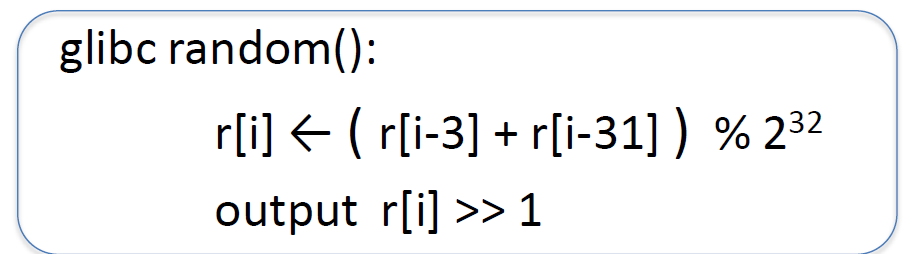
\includegraphics[scale=0.45]{fig1-15.png}\\
%\captionsetup{labelsep=colon}
\caption{}
\end{figure}

Again, this is a very easy generator to predict and should never ever be used for crypto. And so, the lesson I want to emphasize here is never ever use the built-in glibc function random. For crypto, because it doesn't reduce, cryptographic randomness, in the sense that it is easy to predict. And, in fact, systems like Kerberos version four have used random and, have been bitten by that. 
\paragraph{}
So, please don't make that mistake yourself. We will talk about how to do secure random number generation actually in the next lecture. Before we conclude this lecture, I just want to give a little bit more detail about these concepts of negligible and non-negligible values, so different communities in crypto actually define these concepts differently, for practitioners basically these the term negligible and non-negligible, are just, particular scalers that are used in the definition.
\paragraph{} 
A practitioner would say, that if a value is more than one over, one over a billion, one over 230, we say that the value is non-negligible. The reason that's so, is because if you happen to use a key, for example, for, for encrypting a gigabyte of data, a gigabyte of data is about 230 or maybe even $2^{32}$ bytes. Then an event that happens with the probability one over $2^{30}$ will likely happen after about a gigabyte of data. So, since a gigabyte of data is within reason for a particular key, this event is likely to happen. Therefore, one over 230 is non-negligible. 
\paragraph{}
On the other hand, we'll say that one over 280. Which is much, much smaller is an event, an event that happens with this probability is an event that's actually not going to happen over the life of the key. And therefore, we'll say that that's a negligible event. As it turns out, these practical definitions of negligible and non-negligible are quite problematic and we'll see examples of why they're problematic later on. So, in fact in the more rigorous theory of cryptography, the definition of negligible and non-negligible are somewhat different. And in fact, when we talk about the probability of an event, we don't talk about these probabilities as scalars, but rather we talk about them as functions of a security parameter. 
\paragraph{}
So, let me explain what that means. So, these functions, essentially, are functions that map, that outputs, positive real values. So, are non-negative real values that are supposedly probabilities. But they're functions that act on non-negative integers,  So, what does it mean for a function to be non-negligible? What it means is that the function is bigger than some polynomial infinitely often. In other words, for many, for infinitely many values, the function is bigger than some, one over polynomial, okay? So, I wrote the exact definition here, and we'll see an example, in just a minute. 
\begin{equation*}
\epsilon(\lambda):\, \mathrm{nonneg}\, if\quad \exists d:\epsilon(\lambda)\geq\frac{1}{\lambda^d} \qquad
\epsilon\left(\lambda\right):\, \mathrm{negligible\,if}\quad\forall d,\lambda>\lambda_d:\epsilon(\lambda)<\frac{1}{\lambda^d}
\end{equation*}

\paragraph{}
So, if something is bigger, is often bigger than one of that polynomials, we'll say that it's non-negligible. However, if something is smaller than all polynomials, then we'll say that it's negligible. So, what this says here, basically, for any degree polynomial, for all d, there exists some lower bound lambda-d such as, for all lambda bigger than this lambda-d, the function is smaller than one over the polynomial. So, all this says is that the function is negligible if it's less than all polynomial fractions. In other words, is less than one over lambda-d for sufficiently large lambda. 
So, let's look at some examples. And we'll see applications of these negligible and non-negligible concepts later on. But I just want to make, wanted to make it clear that this is how you would rigorously find these concepts. Basically, either smaller than one over poly or bigger than one over poly, one would be negligible, the other would be non-negligible.
\paragraph{}
 Let's look at some examples. So, for example, a function that drops exponentially in ${\lambda}$ clearly would be negligible because for any constant d there is a sufficiently large, large ${\lambda}$. Such as one over $2^{\lambda}$ is less than one over ${\lambda}$ to the d.  So, this is clearly less than all polynomials. Over the function, say, one over ${\lambda}$ to a thousand, right. This is a function that grows very, very slowly. It barely ever moves. Nevertheless, this function is non-negligible because if I set d to be 10,000, then clearly this function is bigger than one over ${\lambda}$ to the 10,000. And so, this function is bigger than some polynomial fraction.
 \paragraph{}
 And let’s look at a confusing example, just to be tricky. What do you think? Suppose I have a function that for an odd ${\lambda}$ it happens to be exponentially small, for even ${\lambda}$, it happens to be polynomially small. Is this a negligible or non-negligible function? Well, by our definition this would a non-negligible function. And the intuition is, if a function happens to be only polynomially small, very often, that actually means that this event, you know, an event that happens with this probability, is already too large to be used in a real cryptosystem.
\paragraph{}
So, the main points to remember here, are that these terms, basically, correspond to less than polynomial or more than polynomial, but throughout the lecture, we'll mostly use negligible to mean less than, than an exponential. And non-negligible to mean, less than one over polynomial. So now we saw the core idea for converting the one-time pad into a practical cipher. And I mean, the stream cipher. And then, in the next lecture, we're going to see how to actually argue that the stream cipher is actually secure. That's going to require a new definition of security, since perfect secrecy is not good enough here, and we will see that in the next lecture.
\begin{figure}[H]
\centering
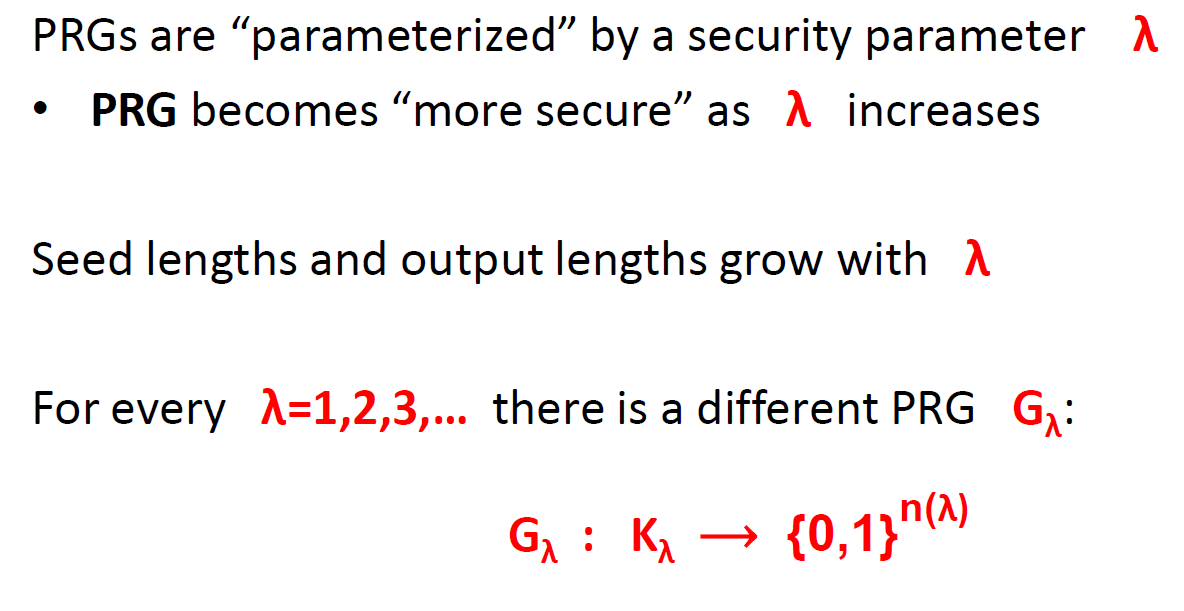
\includegraphics[scale=0.45]{fig1-16.png}\\
%\captionsetup{labelsep=colon}
\caption{}
\end{figure}

\begin{figure}[H]
\centering
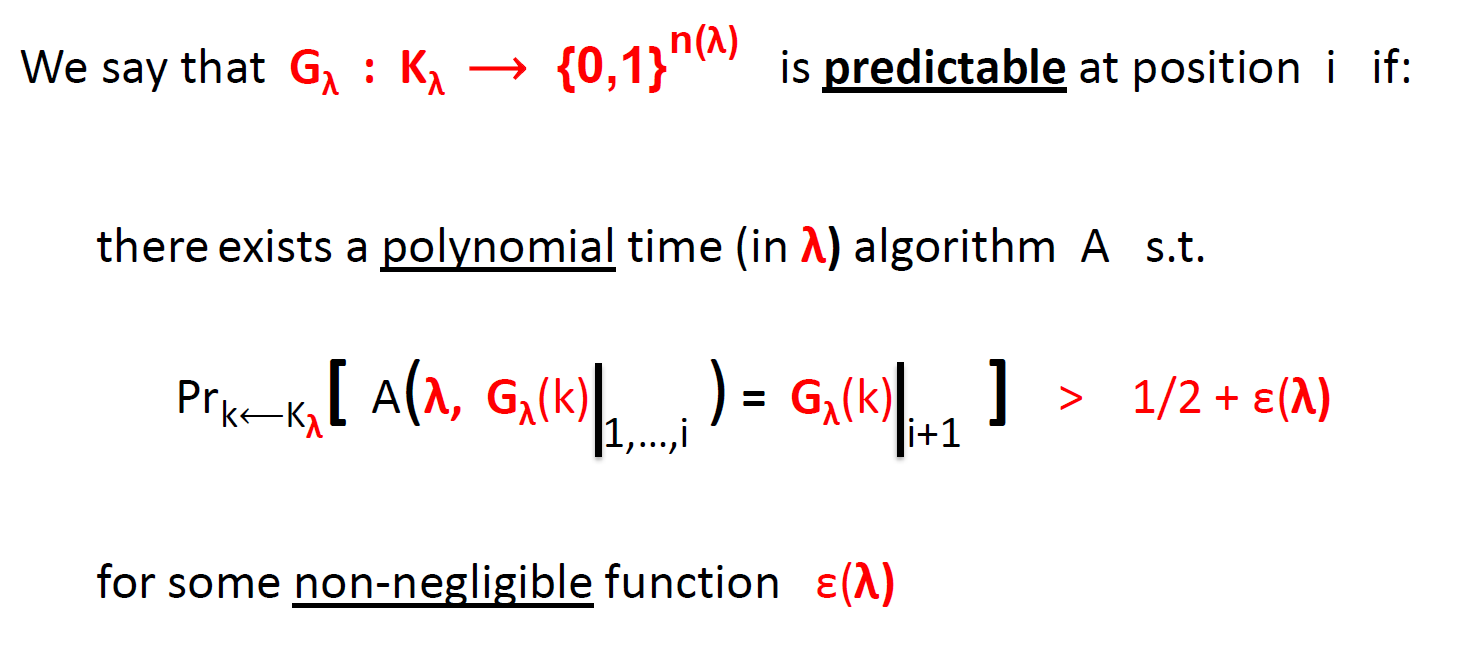
\includegraphics[scale=0.45]{fig1-17.png}\\
%\captionsetup{labelsep=colon}
\caption{}
\end{figure}

\section{Stream Ciphers 2: Attacks and common mistakes}
\subsection{Attacks on Stream Ciphers and The One-Time Pad}
\paragraph{}
In this part, we're going to look at attacks on the one-time pad, and so, let me tell you things you need to be careful with when you use the stream cipher. But before we do that, let's do a quick review of where we were. So, recall that the one-time pad encrypts messages by XORing the message and a secret key, where the secret key is as long as the message. Similarly, decryption is done by similarly XORing the cipher text, and the same secret key. When the key is uniform and random, we prove that the one-time pad has this information theoretic security that Shannon called perfect secrecy. A problem was, of course, the keys are as long as the message, So, the one-time pad is very difficult to use.
\paragraph{}
  
We then talked about a way to make the one-time pad practical by using a pseudo random generator that expands a short seed into a much larger message and the way a stream cipher worked, essentially using a pseudo random generator, was in the same way as the one-time pad, basically, but rather than using a truly random pad, we used this pseudo random pad that's expanded to be as long as the message from the short key that's given as input to the generator. We said now the security no longer relies on perfect secrecy because stream ciphers cannot be perfectly secure. Instead, security relies on properties of the pseudo random generator and we said that the pseudo random generator essentially needs to be unpredictable, but in fact it turns out that definition is a little bit hard to work with and we're going to see a better definition of security for \textbf{PRGs} in about two segments.

\paragraph{} But in this segment, we're going to talk about attacks on the one-time pad. And the first attack I want to talk about is what's called the two-time pad attack, okay? So, remember that the one-time pad is called "one-time" pad because the pad can only be used to encrypt a single message. I want to show you that if the same pad is used to encrypt more than one message, then security goes out the window, and basically an eavesdropper can completely decrypt encrypted messages. So, let's look at an example. So, here we have two messages $m_1$ and $m_2$ that are encrypted using the same pad. So, the resulting ciphertext, $C_1$ and $C_2$, again basically are encryptions of these messages, $m_1$ and $m_2$, but both are encrypted using the same pad. Now suppose an eavesdropper intercepts $C_1$ and $C_2$, and he obtains, he basically has both $C_1$ and $C_2$. The natural thing for the eavesdropper to do is actually compute the XOR of $C_1$ and $C_2$ and what does he get when he computes this XOR? So, I hope everybody sees that, basically, once you XOR $C_1$ and $C_2$, the pads cancel out, and essentially, what comes out of this is the XOR of the plaintext messages. And it turns out that English basically has enough redundancy, such that if I give you the XOR of two plaintext messages, you can actually recover those two messages completely. 

\begin{equation*}
c_1=k\oplus m_1\quad c_2=k\oplus m_2\Rightarrow c_1\quad c_2=m_1\oplus m_2
\end{equation*}


More importantly for us is these messages are encoded using ASCII. In fact, ASCII encodings has enough redundancy, such that given the XOR of two \textbf{ASCII} encoded messages, you can recover the original messages back. So, essentially, given these XORs, you can recover both messages. So, the thing to remember here is if you ever use the same pad to encrypt multiple messages an attack who intercepts the resulting ciphertexts can eventually recover the existing plaintexts without too much work. So, the stream cipher key or the one-time pad key should never ever be used more than once.
\paragraph{}
 Let's look at Some examples where this comes up in practice. It's a very common mistake to use the stream cipher key, or a one-time pad key more than once. Now, let me show you Some examples where this comes up. So, you know to avoid these mistakes, when you build your own systems. The first example is a historic example. At the beginning of the 1940s, where the Russians actually used a one-time pad to encrypt various messages. Unfortunately, the pads that they were using were generated by a human by throwing dice. And So, you know, the human would throw these dice, and write down the results of these throws. And the collected throws would then form the pads that were used for encryption. Now, because it was kind of laborious for them to generate these pads, it seems wasteful to use the pads to encrypt just one message. So, they ended up using these pads to encrypt multiple messages. And US intelligence was actually able to intercept these two-time pads. These ciphertexts that were encrypted using the same pad, applied to different messages. And it turns out, over a period of several years, they we're able to decrypt Something like 3,000 plain texts just by intercepting these ciphertexts. The project is called Project Venona It's actually a fascinating of cryptanalysis, just because the two-time pad is insecure.
\paragraph{}
 More importantly, I want to talk about more recent examples that come up in networking protocols, So, let me give you an example from Windows NT, in a product called the, point-to-point transfer protocol. This is a protocol for a client wishing to communicate securely with a server. The client and the server both share a secret key here, and they both send messages to one another. So, here, we'll denote the messages from the client by $m_1$. So, the client sends a message, the server responds, the \textbf{client} sends a message, the server responds, the client sends a message, the server responds, and So, on and So, forth.

\begin{figure}[H]
\centering
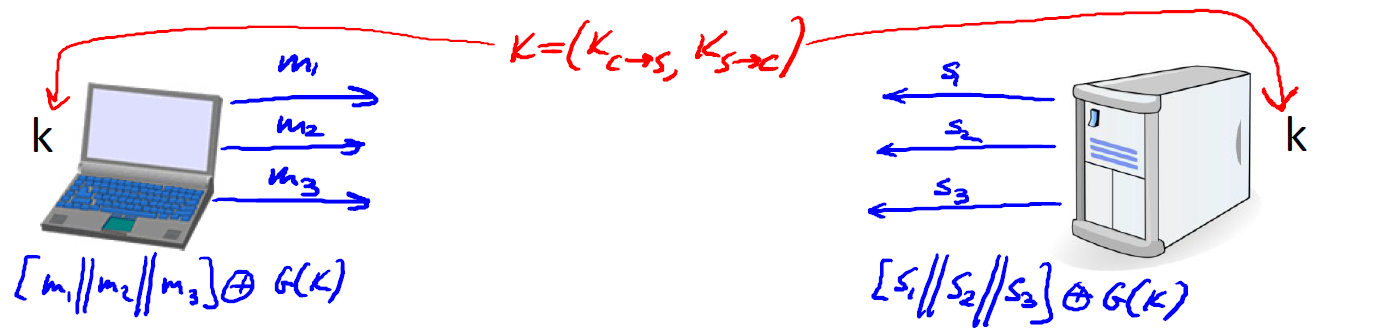
\includegraphics[scale=0.45]{fig1-18.png}\\
%\captionsetup{labelsep=colon}
\caption{}
\end{figure}

\paragraph{}
 Now, the way PPTP works is, basically, the entire interaction, from the client to the server, is considered as one stream. In other words, what happens is, the messages $m_1$, and $m_2$ and $m_3$, are kind of viewed as one long stream. Here, these two parallel lines means concatenation. So, essentially, we're concatenating all the messages from the client to the server into one long stream. And all that stream is encrypted using the stream cipher with key K. So, that's perfectly fine. I mean, there's nothing wrong with that. These messages are encrypted, are treated as one long stream, and they're all encrypted using the same key. The problem is, the same thing is happening also, on the server side. In other words, all the messages from the server are also, treated as one long stream. So, here, they're all concatenated together. And encrypted using, unfortunately, the same pseudo-random seed, in other words, using the same stream cipher key.
\paragraph{}
 So, basically what's happening here is you see an effect that the two-time pad is taking place where the set of messages from the client is encrypted using the same one-time pad as a set of messages from the server. The lesson here is that you should never use the same key to encrypt traffic in both directions. In fact, what you need to do is have one key for interaction between the client and the server and one key for interaction between the server and the client. The way I like to write this is really that the shared key k really is a pair of keys. One key is used to encrypt messages from server to client, and one key is used to encrypt messages from client to server. So, \underline{these are two separate keys} that are used, and both sides, of course, know this key. Both sides have this pair of keys, and they can both encrypt. So, one is used to encrypt messages in one direction and one is used to encrypt messages in the other direction.
\paragraph{}
Another important example of the two-time pad comes up in Wi-Fi communication, particularity in the 80211B protocol. So, all of you I'm sure know that the 80211 contains an encryption layer and the original encryption layer was called WEP and WEP fortunately for us is actually a very badly designed protocol So, that I can always use it as an example of how not to do things. There are many mistakes inside of WEP and here I want to use it as an example of how the two-time pad came about. 

\begin{figure}[H]
\centering
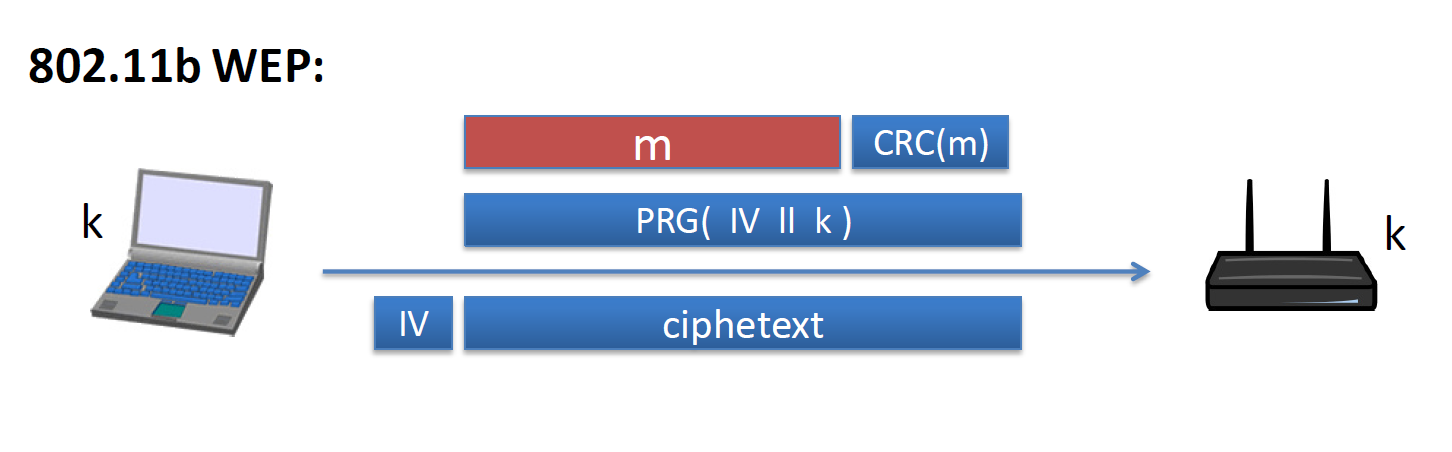
\includegraphics[scale=0.45]{fig1-19.png}\\
%\captionsetup{labelsep=colon}
\caption{}
\end{figure}

\paragraph{}So, let me explain how WEP works. So, in WEP, there's a client and, and access point. Here's the client, here's the access point. They both share a secret key K. And then, when they want to transmit a message to one another. Say these are frames, that they transmit to one another. Let's say the client wants to send. A frame containing the plain text M to the axis point, what he would do is first of all he appends Some Sort of check sum to this plain text. The check sum is not important at this point, what is important is then this new calculation gets encrypted using a stream cipher where the stream cipher key is this concatenation of a value IV and a long-term key K. So, this IV is a 24-bit string.  This IV is a 24-bit string, and you can imagine that it starts from zero and perhaps it's a counter that counts increments by one for every packet. The reason they did this was the designers of Wep realized that in a stream cipher, the key is only supposed to be used to encrypt one message. So, they said well, let's go ahead and change the key after every frame. And the way they changed the key essentially was by prepending this IV to it. And you notice this IV changes on every packet. So, it increments by one on every packet. And the idea, then, is sent in the clear along with the ciphertext. 
So, the recipient knows the key K. He knows what the IV is. He can rederive the \textbf{PRG} of IV concatenating K. And then decrypts the cipher text to recover the original message M. Now the problem with this of course is the IV is only 24 bits long. Which means that there are only $2^{24}$ possible IV's. Which means that after sixteen million frames are transmitted. Essentially the IV has to cycle. And once it cycles after 60 million frames. Essentially, we get a two-time path. The same IV will be used to encrypt two different messages. The TK never changes. It's a long-term key. And as a result, that same key, namely the IV concatenated K would be used to encrypt two different frames, and the attacker can then figure out the plain text of both frames.
\paragraph{}
 So, that's one problem. And the worst problem is in fact that on many 80211 cards, if you power cycle the card, the IV will reset back to zero. And as a result, every time you power cycle the card, essentially, you'll be encrypting the next payload using zero concatenated K So, after every power cycle, you'll be using the zero concatenated K key to encrypt many times the same packets. So, you see how in WEP, the same pad could be used to encrypt many different messages as Soon as the IV is repeated. There is nothing to prevent the IV from repeating after a power cycle. 
Repeating after every sixteen million frames which isn't that many frames in a busy network.
\paragraph{}
 So, while we are talking about WEP. I want to mention one more mistake that was done in WEP. This is a pretty significant mistake and let's see how we might design it better. So, you notice that the designers of WEP basically wanted to use a different key for every packet.  So, every frame is encrypted using a different key is concatenation of IV and K. Unfortunately. They didn't randomize the keys and the keys are actually, if you look at the key for frame number one, well, you know, it will be this concatenation of one and k. We'll just feel these 24 bits. Then the key for frame number two is the concatenation of two and k. The key for frame number three is the concatenation of three and k. So, the keys are very closely related to one another. And I should probably mention also, that these keys themselves can be 104 bits So, that the resulting \textbf{PRG} key. Is actually 104 plus 24 bytes which is 128 bytes. Unfortunately, these keys are very much related to one another. These are not random keys. You notice they all have the same suffix of 104 bytes. And it turns out the pseudo-random generator used in Wep is not designed to be secure when you use related keys that are So, closely related. In other words, the majority of these keys are basically the same. And in fact, for the \textbf{PRG} that's used in WEP. That \textbf{PRG} is called, RSC four. We'll talk about that more in the next part. 
\paragraph{}
It turns out there's an attack. It was discovered by Fluhrer, Mantin and Shamir back in 2001, that shows that after about ten to the six of, after about a million frames. You can recover the secret key. So, this is kind of a disastrous attack that says essentially all you have to do is listen to a million frames. These frames basically. As we said they're all generated from a very common seed, namely 104 bits of these seeds are all the same. The fact that they've used such closely related keys is enough to actually recover the original key. And it turns out even after the 2001 attack, better attacks have come out that show that these related keys are very much disastrous and in fact these days Something like 40,000 frames are sufficient. And So, that, within a matter of minutes, you can actually recover the secret key in any WEP network. 

\paragraph{}
So, WEP provides no security at all for two reasons. First of all, it can resolve in the two-time pad. But more significantly, because these keys are so, closely related, it's actually possible to recover the key by watching just a few cipher texts. And by the way, we'll see that well, when we do a security analysis of these steps of constructions. In a few segments, we'll start talking about how to analyze these steps of constructions. We'll see that when we have related keys like this, in fact, our security analysis will fail. We won't be able to get the proof to go through. 
\paragraph{}
One could ask what should the designers of a WEP should have done, instead? Well, one approach is to basically treat the frames, you know $m_1$, $m_2$, $m_3$. Each, each one is a separate frame transmitter from the client to the server. He could have treated them as one long stream, and then XOR them potentially. Using the pseudo random generator as one long stream. So, the first segment of the pad would have been used to encrypt $m_1$. The second segment of the pad would have been used to encrypt $m_2$. The third segment of the pad would have been used to encrypt $m_3$. And So, on and So, forth. So, they basically could never have had to change the key because the entire interaction is viewed as one long stream. But they chose to have a different key for every frame. So, if you want to do that, a better way to do that is, rather than slightly modifying this IV that just slightly modifies the prefix of the key, of the PRG key. A better way to do that is to use a \textbf{PRG} again. So, essentially, what you could do is you will take your long-term key. And then feed that directly through a \textbf{PRG}. 

\begin{figure}[H]
\centering
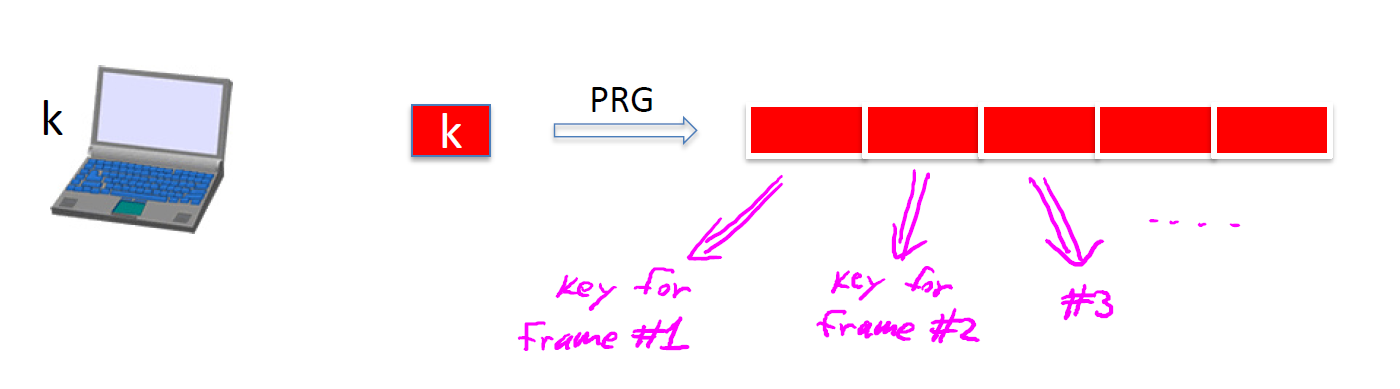
\includegraphics[scale=0.45]{fig1-20.png}\\
%\captionsetup{labelsep=colon}
\caption{}
\end{figure}

\paragraph{}
So, now we get a long stream of bits that look essentially random. And then the initial segment could be used, the first segment could be used as the key, or frame number one. And then the second segment would be used as the key for, you know, key for frame number two. And So, on and So, forth. The third segment would be used to encrypt frame \# three and So, on and So, forth, okay? So, the nice thing about this is now, essentially, by doing this, each frame has a pseudo-random key. These keys, now, have no relation to one another. They look like random keys. And as a result, if the \textbf{PRG} is secure for random Cs, it was also, be secure on this input. Because these keys essentially look as though they're independent of one another.
\paragraph{}We'll see how to do this analysis formally once we talk about these types of constructions. Since this two-time pad attack comes up So, often in practice, it's such a common mistake, I want to give one more example where it comes up so, you know how to avoid it. 
\paragraph{}
The last example I want to give is in the context of disk encryption. So, imagine we have a certain file and maybe the file begins with, you know, the words to Bob. And then the contents of the file follow when this is stored on disk of course the file is going to get So, here we have our disk here, the file is going to get broken into blocks. And each block will be, you know, when we actually store this on a disk, you know, things will be encrypted. You know, So, maybe to Bob will go into the first block and then the rest of the content will go into the remaining blocks. And an attacker looking at the disk has no idea what the contents of the message is. But now suppose that at a later time, user goes ahead and modifies, basically fires up the editor. It modifies the file, So, now instead of saying to Bob, it says to Eve. And nothing else changes in the file, that's the only change that was made. 
\paragraph{}
When the user then saves this modified file to disk, basically he's going to \textbf{re-encrypt} it again. And So, the same thing is going to happen. The file is going to get broken into blocks. You know, now the file's going to say to Eve. And everything, of course, is going to be encrypted. So, again, I'll, put these lines here. Now an attacker looking at the disc, taking a snapshot of the disc before the edits. And then looking again at the disc after the edits. What he will see is that the only thing that changed is this little segment here. That's now different. Everything else looks exactly the same. So, the attacker, even though he doesn't know what actually happened to the file within the file or what changed, he knows exactly the location where the edits took place.
 And So, the fact that the one-time path or a stream cipher encrypts one bit at a time means that if one change takes place, then it's very easy to tell where that change occurred instantly. That leaks information that the attacker shouldn't actually learn. Ideally, you'd like to say that even if the file changed just a little bit. Entire contents of the file should change. Or maybe at least the entire contents of the blocks should change. Here you can see the attacker even knows within the block where the change was actually made, okay. 
\paragraph{}
So, in fact, because of this, it's usually a bad idea to use stream ciphers for disk encryption. And essentially this is another example of a two-time pad attack because the same pad is used to encrypt two different messages. This, they happen to be very similar, but nevertheless these are two different messages, and the attacker can learn what the change was and in fact he might be able to even learn what the actual changed words were, as a result of this.  So, the lesson here is generally we need to do something different for disk encryption. We'll talk about what to do for disk encryption in a later segment, but essentially the one-time pad is generally not a good idea for encrypting blocks on disks. 
\paragraph{}
So, just again to summarize the two-time pad attack, we saw that you're supposed, I hope I've convinced you that you're never ever, ever supposed to use a stream cipher key more than once. Even though there are natural settings where that might happen, you have to take care and make sure that you're not using the same key more than once. So, for network traffic typically what you're supposed to do is every session would have its own key. Within the session the message from the client and the server look as one complete stream. It would be encrypted using one key. Is, the messages from the server to the client would be treated as one stream and encrypted using a different key. And then for this encryption typically would not use a stream cipher because. As changes are made to the file, he would be leaking information about the contents of the file. So, that concludes our brief discussion of the two-time pad. 
\paragraph{}
Next attack I want to mention , Is a fact that the one-time path and stream ciphers in general provide no integrity at all. All they do is they try to provide confidentiality when the key is only used once. They provide no integrity at all but even worse than that it's actually very easy to modify cipher text and have known effects on the corresponding plain text. So, let me explain what I mean by that. This property, by the way, is called malleability, and we'll see what I mean by that in just a second. 


\begin{figure}[H]
\centering
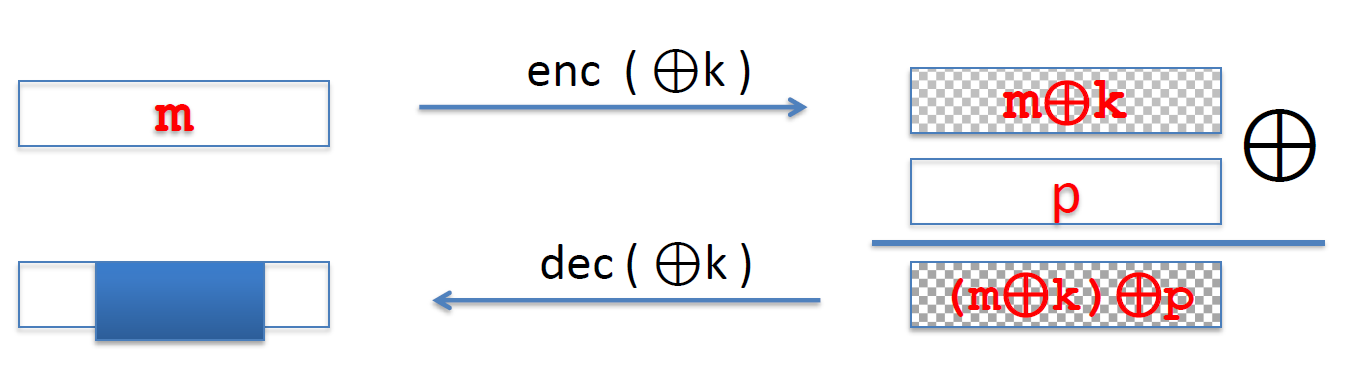
\includegraphics[scale=0.45]{fig1-21.png}\\
%\captionsetup{labelsep=colon}
\caption{}
\end{figure}

\paragraph{}
So, imagine we have Some message M that gets encrypted. Here, it gets encrypted using a stream cipher. And the cipher text, of course, is then going to be, M XOR a K. Now an attacker intercepts the cipher text. Well, that doesn't tell him what's, what the plain text is but what he can do is now beyond eavesdropping he can actually become an active attacker and modify the cipher text. So, when I say modify the cipher text let's suppose that he XOR the cipher text with a certain value P. What’s called a sub-permutation key. Well, the resulting cipher text then becomes M XOR K, XOR P. So, now I'll ask you, when we decrypt the cipher text, what is it going to decrypt to?
\paragraph{}
 Well, I hope everybody sees manipulating the XORs Basically the decryption becomes M XOR P So, you notice that by XOR with this pad P, the attacker was able to have a very specific effect on the resulting plain text.  So, a summary is basically you can modify the cipher text. These modifications are undetected. But even worse, they're undetected, they have a very specific impact on the resulting plain text. Namely whatever you XOR the cipher text with is going to have that exact effect on the plain text. 
\paragraph{}
So, to see where this can be dangerous, let's look at a particular example. Suppose the user sends an email that starts with the words from Bob. In the attacker intercepts the corresponding cipher text. He doesn't know what the cipher text is but let's just for the sake of it let's pretend that he actually knows that this message is actually from Bob. What he wants to do is he wants to modify the ciphertext So, that the plain text would now look like it came from Somebody else. Say, he wants to make it look like this message actually came from Alice. All he has is the ciphertext. Well, what he can do is he can XOR with a certain three characters. We'll see what those three characters are in just a second. And such that the resulting ciphertext is actually an encryption of the message from Eve. And So, that now when the user decrypts that. All of a sudden, he'll see, Hey, this message is from Eve. It's not, he'll think this message is from Eve, not from Bob. And that might cause you know, the wrong thing to take place. So, here the attacker, even though he himself could not have created a cipher text that says from Eve, by modifying an existing cipher text all of a sudden, he was able to make the cipher text that he could not have done without intercepting at least one cipher text. So, again by intercepting one cipher text he was able to change it So, not it looks like it's from Eve, rather than from Bob. 

\begin{figure}[H]
\centering
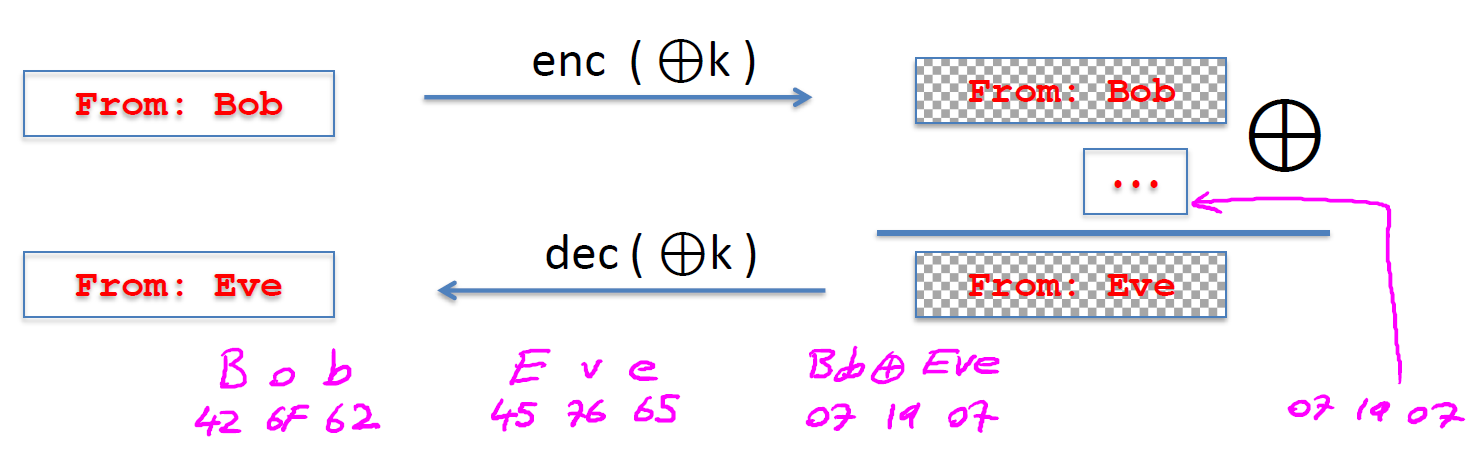
\includegraphics[scale=0.45]{fig1-22.png}\\
%\captionsetup{labelsep=colon}
\caption{}
\end{figure}

So, just to be specific, let's look what these three characters need to be, So, let's look at the word Bob. And I'm going to write it in ASCII. So, Bob in ASCII corresponds to 42 hex six f hex and 62 hex. So, little b is encoded as 62, little o is encoded as six f. The word eve is encoded as 45 hex, 76 hex, and 65 hex. Now when I XOR these two words, I'm literally going to x over them as bit strings. So, Bob XOR eve, it's not difficult to see that what I get are the three characters zero, seven. Nineteen and 07. So, really what these three characters here are going to be. Are simply 07, nineteen, and 07. And by XORing these three characters at the right positions into the cipher text, the attacker was able to chance the cipher text to look like it came from Eve rather than from Bob. So, this is an example where having a predictable impact on the cipher text can actually cause quite a bit of problems. And this is this property called malleability. And we say that the one-time pad is malleable because it's very easy to compute in cipher texts, and make prescribed changes to the corresponding plain text. So, to prevent all this, I'm going to do that, actually, in two or three lectures. And we're going to basically show how to add integrity to encryption mechanisms in general. But right now, I want you to remember that the one-time pad by itself has no integrity and is completely insecure against attackers that actually modify the cipher texts.

\section{Stream Ciphers 3: Real-world examples}
\subsection{Real-world Stream Ciphers}
\paragraph{}
In this part, I want to give a few examples of stream ciphers that are used in practice. I'm going to start with two old examples that actually are not supposed to be used in new systems. But nevertheless, they're still fairly widely used, and so, I just want to mention the names so, that you're familiar with these concepts. 
The first stream cipher I want to talk about is called \textbf{RC4}, designed back in 1987. And I'm only going to give you the high-level description of it, and then we'll talk about some weaknesses of \textbf{RC4} and leave it at that. So, \textbf{RC4} takes a variable size seed, here I just gave as an example where it would take 128 bits as the seed size, which would then be used as the key for the stream cipher. The first thing it does, is it expands the 128-bit secret key into 2,048 bits, which are going to be used as the internal state for the generator. And then, once it's done this expansion, it basically executes a very simple loop, where every iteration of this loop outputs one byte of output. So, essentially, you can run the generator for as long as you want, and generate one byte at a time. Now \textbf{RC4} is actually, as I said, fairly popular. It's used in the HTTPS protocol quite commonly actually. These days, for example, Google uses \textbf{RC4} in its HTTPS. It's also, used in WEP as we discussed in the last part, but of lecture in WEP, it's used incorrectly and it's completely insecure the way it's used inside of WEP.

\begin{figure}[H]
\centering
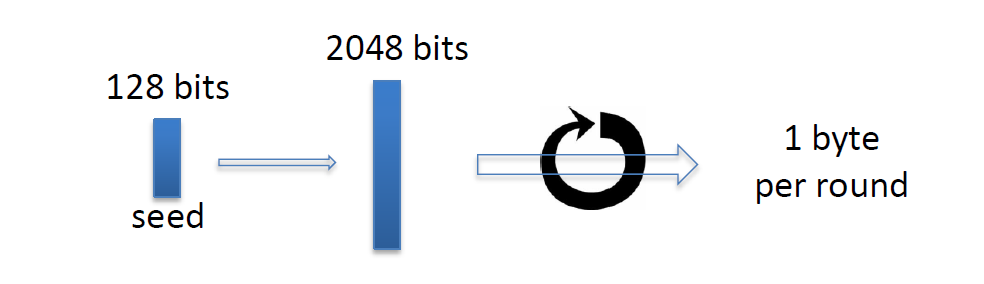
\includegraphics[scale=0.45]{fig1-23.png}\\
%\captionsetup{labelsep=colon}
\caption{}
\end{figure}
 \paragraph{}
 So, over the years, some weaknesses have been found in RC4, and as a result, it's recommended that new projects actually not use RC4 but rather use a more \underline{modern pseudo-random generator} as we'll discuss toward the end of the segment. Let me just mention two of the weaknesses. The first one is, it's kind of bizarre basically, if you look at the second byte of the output of RC4. It turns out the second byte is slightly biased. If RC4 was completely random, the probability that the second byte happens to be equal to zero would be exactly one over 256. There are 256 possible bytes, the probability that it's zero should be one over 256. It so, happens that for RC4 the probability is actually two over 256, which means that if you use the RC4 output to encrypt a message the second byte is likely to not be encrypted at all. In other words it'll be XOR-ed with zero with twice the probability that it's supposed to. So, two over 256, instead of one over 256. And by the way I should say that there's nothing special about the second byte. It turns out the first and the third bytes are also, biased. And in fact, it's now recommended that if you're going to use RC4, what you should do is ignore basically the first 256 bytes of the output and just start using the output of the generator starting from byte 257. The first couple of bytes turned out to be biased, so, you just ignore them. 
 \paragraph{}
The second attack that was discovered is that in fact if you look at a very long output of RC4 it so, happens that you're more likely to get the sequence 00. In other words, you're more likely to get sixteen bits, two bytes of 00, than you should. Again, if RC4 was completely random the probability of seeing 00 would be exactly 1/256 squared. It turns out RC4 is a little biased and the bias is 1/256 cubed. It turns out this bias actually starts after several gigabytes of data are produced by RC4. But nevertheless, this is something that can be used to predict the generator and definitely it can be used to distinguish the output of the generator from a truly random sequence. Basically, the fact that 00 appears more often than it should is the distinguisher. And then in the last segment we talked about related-key attacks that were used to attack WEP, that basically say that if one uses keys that are closely related to one another then it's actually possible to recover the root key. These are the weaknesses that are known of RC4 and, as a result, it's recommended that new systems actually not use RC4 and instead use a modern pseudo-random generator. 
\paragraph{}
Second example I want to give you is a badly broken stream cipher that's used for encrypting DVD movies. When you buy a DVD in the store, the actual movie is encrypted using a stream cipher called the \textbf{\textit{Content Scrambling System}}, \textbf{CSS} turns out to be a badly broken stream cipher, and we can very easily break it, and I want to show you how the attack algorithm works. We're doing it so, you can see an example of an attack algorithm, but in fact, there are many systems out there that basically use this attack to decrypt encrypted DVDs.
\paragraph{} 
The \textit{CSS} stream cipher is based on something that hardware designers like. It's designed to be a hardware stream cipher that is supposed to be easy to implement in hardware, and is based on a mechanism called a \underline{Linear Feedback Shift Register}. So, a linear feedback shift register is basically a register that consists of cells where each cell contains one bit. Then basically what happens is there are these taps into certain cells, not all the cells, certain positions are called taps. And then these taps feed into an XOR and then at every clock cycle, the shift register shifts to the left. The last bit falls off and then the first bit becomes the result of this XOR. You can see that this is a very simple mechanism to implement, and in hardware takes very few transistors. Just the shift right, the last bit falls off and the first bit just becomes the XOR of the previous bits. So, the seed for this \textbf{LFSR} basically, is the initial state of the LFSR. And it is the basis of a number of stream ciphers. 
\paragraph{}
As I said, DVD encryption uses two LFSRs. I'll show you how that works in just a second. \textbf{GSM} encryption, these are algorithms called A51 and A52 , $ ( A5\backslash 1,2 ) $. And that uses three LFSRs. Bluetooth encryption is an algorithm called, E0. These are all stream ciphers, and that uses four LFSRs. Turns out all of these are badly broken, and actually really should not be trusted for encrypting traffic, but they're all implemented in hardware, so, it's a little difficult now to change what the hardware does. But the simplest of these, CSS, actually has a cute attack on it, so, let me show you how the attack works.

\begin{figure}[H]
\centering
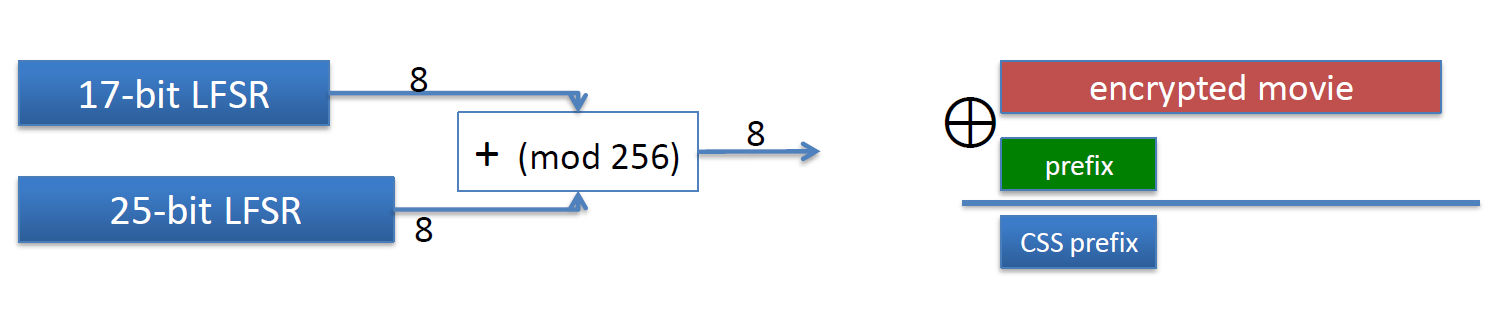
\includegraphics[scale=0.45]{fig1-24.png}\\
%\captionsetup{labelsep=colon}
\caption{}
\end{figure}
 
 \paragraph{}
Let's describe how CSS actually works. The key for CSS is five bytes, namely 40 bits, five times eight is 40 bits. The reason they had to limit themselves to only 40 bits is that DVD encryption was designed at a time where U.S. Export regulations only allowed for export of crypto algorithms where the key was only 40 bits. So, the designers of CSS were already limited to very, very short keys. Just 40-bit keys. Their design works as follows. Basically, CSS uses two LFSR's. One is a 17-bit LFSR. In other words, the register contains 17 bits. And the other one is a 25-bit LFSR, it's a little bit longer, 25-bit LFSR. And the way these LFSRs are seeded is as follows. The key for the encryption, basically looks as follows. You start off with a one, and you concatenate to it the first two bytes of the key. And that's the initial state of the LFSR. And then the second LFSR basically is initialized the same way. “1” concatenated the last three bytes of the key. And that's loaded into the initial state of the LFSR. 
\\
Initial of 17-bit LFSR: 1||first two bytes of the key\\
Initial of 25-bit LFSR: 1||last three bytes of the key\\
\paragraph{}
You can see that the first two bytes are 16 bits, plus leading 1, that's 17 bits overall, whereas the second LFSR is 24 bits plus 1 which is 25 bits. And you notice we used all five bits of the key. So, then these LFSRs are basically run for eight cycles, so, they generate eight bits of output. And then they go through this adder that does basically addition modulo 256. Yeah so, this is an addition box, modulo 256. There's one more technical thing that happens. Also, added is the carry from the previous block. But that is not so, important. That's a detail that's not so, relevant.  Every block, you notice we're doing addition modulo 256 and we're ignoring the carry, but the carry is basically added as a zero or a one to the addition of the next block.  And then basically this output one byte per round.  And then this byte is then of course used, XOR-ed with the appropriate byte of the movie that's being encrypted. 
\paragraph{}
It's a very simple stream cipher, it takes very little hardware to implement. It will run fast, even on very cheap hardware and it will encrypt movies. It turns out this is easy to break in time roughly 217. Now let me show you how. So, suppose you intercept the movies, so, here we have an encrypted movie that you want to decrypt. So, let's say that this is all encrypted so, you have no idea what's inside of here. However, it so, happens that just because DVD encryption is using MPEG files, it so, happens if you know of a prefix of the plaintext, let's just say maybe this is twenty bytes. Well, we know if you XOR these two things together, so, in other words, you do the XOR here, what you'll get is the initial segment of the PRG. So, you'll get the first twenty bytes of the output of CSS, the output of this PRG. Now here's what we're going to do. We have the first twenty bytes of the output. Now we do the following. 
\paragraph{}
We try all $2^{17}$ possible values of the first LFSR.  So, 217 possible values. For each value, so, for each of these $2^{17}$ initial values of the LFSR, we're going to run the LFSR for twenty bytes,  We'll generate twenty bytes of outputs from this first LFSR, assuming—for each one of the 217 possible settings. Now, remember we have the full output of the CSS system. What we can do is we can take this output that we have. And subtract it from the twenty bites that we got from the first LFSR, and if in fact our guess for the initial state of the first LFSR is correct, what we should get is the first twenty-byte output of the second LFSR. Because that's by definition what the output of the CSS system is. 
\paragraph{}
Now, it turns out that looking at a 20-byte sequence, it's very easy to tell whether this 20-byte sequence came from a 25-bit LFSR or not. If it didn't, then we know that our guess for the 17-bit LFSR was incorrect and then we move on to the next guess for the 17-bit LFSR and the next guess and so, on and so, forth. Until eventually we hit the right initial state for the 17-bit LFSR, and then we'll actually get, we'll see that the 20 bytes that we get as the candidate output for the 25-bit LFSR is in fact a possible output for a 25-bit LFSR. And then, not only will we have learned the correct initial state for the 17-bit LFSR, we will have also, learned the correct initial state of the 25-bit LFSR. And then we can predict the remaining outputs of CSS, and of course, using that, we can then decrypt the rest of the movie. We can actually recover the remaining plaintext. 
\paragraph{}
 This is things that we talked about before. We're also, going to be doing a homework exercise on this type of stream ciphers and you'll kind of get the point of how these attack algorithms work. And I should mention that there are many open-source systems now that actually use this method to decrypt CSS-encrypted data. 
\paragraph{}
Now that we've seen two weak examples, let's move on to better examples, and in particular the better pseudo-random generators come from what's called the \underline{eStream Project}. This is a project that concluded in 2008, and they qualify basically five different stream ciphers, but here I want to present just one. First of all the parameters for these stream ciphers are a little different than what we're used to. These stream ciphers as normal they have a seed. But in addition, they also have, what's called a nonce and we'll see what a nonce is used for in just a minute. They take two inputs a seed and a nonce. We'll see what the nonce is used for in just a second. And the of course they produce a very large output, so, n here is  much, much bigger than s. Now, when I say \textbf{nonce}, what I mean is a value that's never going to repeat as long as the key is fixed. And I'll explain that in more detail in just a second. But for now, just think of it as a unique value that never repeats as long as the key is the same. And so, of course once you have this PRG, you would encrypt, you get a stream cipher just as before, except now as you see, the PRG takes as input both the key and the nonce. And the property of the nonce is that the pair, (k,r) never repeats. It's never used more than once. So, the bottom line is that you can reuse the key, because the nonce makes the pair unique, because (k,r) are only used once. I'll say they're unique. This nonce is kind of a cute trick that saves us the trouble of moving to a new key every time. 
\paragraph{}
The particular example from the eStream that I want to show you is called \underline{Salsa twenty}. It's a stream cipher that's designed for both software implementations and hardware implementations. It's kind of interesting. You realize that some stream ciphers are designed for software, like RC4. Everything it does is designed to make software implementation run fast, whereas other stream ciphers are designed for hardware, like CSS, using an LFSR that's particularly designed to make hardware implementations very cheap. It's also, the nice thing about that is that it's designed so, that it's both easy to implement it in hardware and its software implementation is also, very fast. 
\paragraph{}
Let me explain how Salsa works. Well, Salsa takes either 128 or 256-bit keys. I'll only explain the 128-bit version of Salsa. This is the seed. And then it also, takes a nonce, just as before, which happens to be 64 bits. And then it'll generate a large output. Now, how does it actually work? Well, the function itself is defined as follows. Basically, given the key and the nonce, it will generate a very long, well, a long pseudorandom sequence, as long as necessary. And it'll do it by using this function that I'll denote by H. This function H takes three inputs. Basically the key. Well, the seed k, the nonce r, and then a counter that increments from step to step. So, it goes from zero to one, two, three, four as long as we need it to be.  So, basically, by evaluating this h on this k r, but using this incrementing counter, we can get a sequence that's as long as we want. So,  all I have to do is describe how this function H works. Now, let me do that here for you. The way it works is as follows. Well, we start off by expanding the states into something quite large which is 64 bytes long, and we do that as follows. We stick a constant at the beginning, so, there's $\tau_0$, these are four bytes, it's a four-byte constant, so, the spec for Salsa basically gives you the value for $\tau_0$. Then we put k in which is 16 bytes. Then we put another constant. Again, this is four bytes. And as I said, the spec basically specifies what this fixed constant is. Then we put the nonce, which is eight bytes. Then we put the index. This is the counter zero, one, two, three, four, which is another eight bytes. Then we put another constant $\tau_2$, which is another four bytes. Then we put the key again, this is another sixteen bytes. And then finally we put the third constant, $\tau_3$, which is another four bytes. 

\begin{figure}[H]
\centering
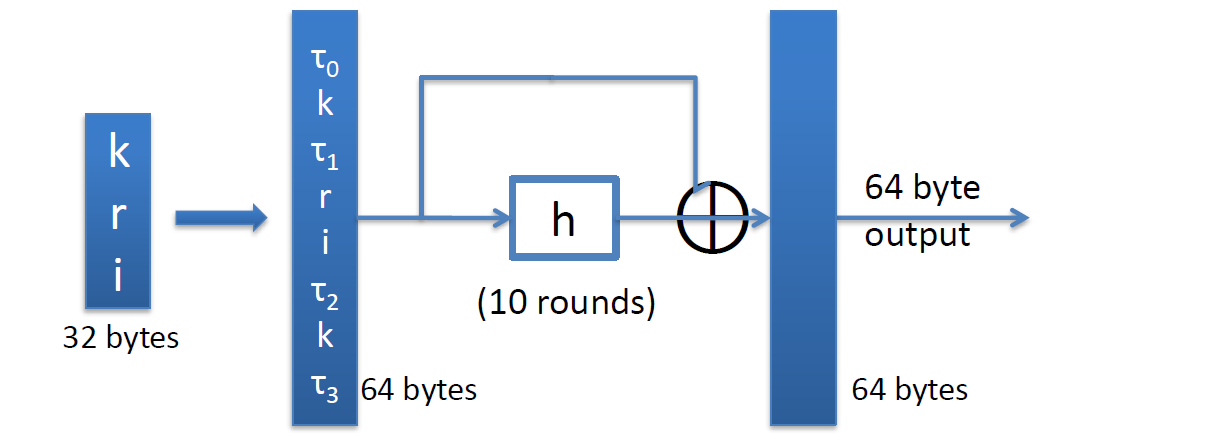
\includegraphics[scale=0.45]{fig1-25.png}\\
\captionsetup{labelsep=colon}
\caption{The CSS Stream Cipher}
\end{figure}
  
\paragraph{}
As mentioned, if you sum these up, you see that you get 64 bytes. We've expanded the key and the nonce and the counter into 64 bytes. The key is repeated twice I guess. And then what we do is we apply a function, I'll call this functional little h. Okay, so, we apply this function, little h. And this is a function that's one to one so, it maps 64 bytes to 64 bytes. It's a completely invertible function. Given the input you can get the output and given the output you can go back to the input. And it's designed specifically so, it's a- easy to implement in hardware and b- on an x86, it's extremely easy to implement because x86 has this SSE2 instruction set which supports all the operations you need to do for this function. It's very, very fast. As a result, Salsa has a very fast stream cipher. And then it does this basically again and again. 
\paragraph{}
It applies this function h again and it gets another 64 bytes. And so on and so, forth, basically it does this ten times. Okay so, the whole thing here, say repeats ten times, so, apply h ten times. And then by itself, this is actually not quite random. It's not going to look random because like we said, H is completely invertible. Given this final output, it's very easy to just invert h and then go back to the original inputs and then test that the input has the right structure. You do one more thing, you do an addition word by word. So, if there are 64 bytes, you do a word-by-word addition four bytes at a time, and finally you get the 64-byte output, and that's it. That's the whole pseudo-random generator. So, that's the whole function, little h. And as I explained, this whole construction here is the function big H. And then you evaluate big H by incrementing the counter I from zero, one, two, three onwards. And that will give you a pseudo-random sequence that's as long as you need it to be. 
\paragraph{}
And basically, there are no significant attacks on this. This has security that's very close to 2128. We'll see what that means more precisely later on. It's a very fast stream cipher, both in hardware and in software. And, as far as we can tell, it seems to be unpredictable as required for a stream cipher. 
\paragraph{}
So, I should say that the eStream project actually has five stream ciphers like this. I only chose Salsa because I think it's the most elegant. But I can give you some performance numbers here. You can see, these are performance numbers on a 2.2 gigahertz, you know, x86 type machine. And you can see that RC4 actually is the slowest. Because essentially, well it doesn't really take advantage of the hardware. It only does byte operations. And so, there's a lot of wasted cycles that aren't being used. But the E-Stream candidates, both Salsa and other candidate called Sosemanuk. I should say these are eStream finalists. These are actually stream ciphers that are approved by the eStream project. You can see that they have achieved a significant rate. This is 643 megabytes per second on this architecture, more than enough for a movie and these are actually quite impressive rates. 


\begin{figure}[H]
\centering
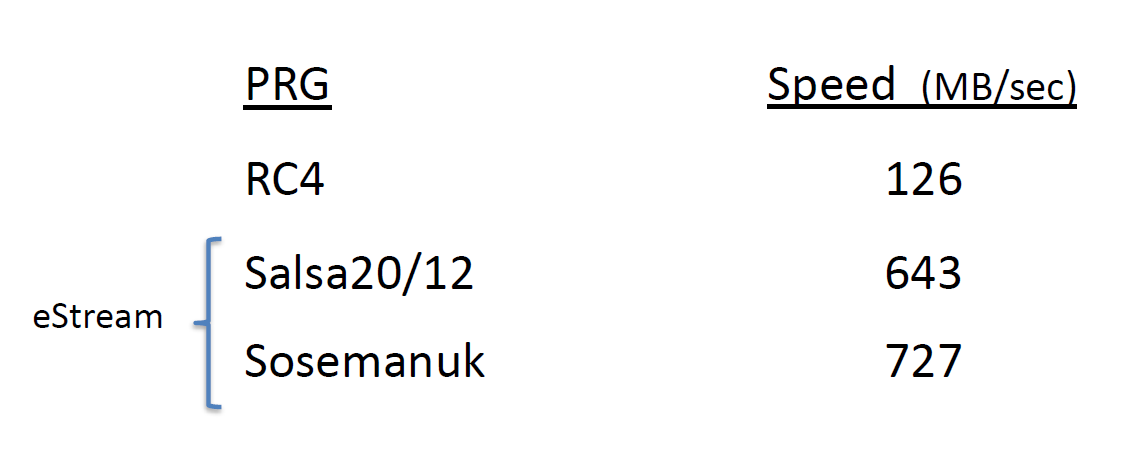
\includegraphics[scale=0.45]{fig1-26.png}\\
\captionsetup{labelsep=colon}
\caption{Performance on AMD Operton, 2.2 GHz, linux}
\end{figure}

\paragraph{}
And so, now you've seen examples of two old stream ciphers that shouldn't be used, including attacks on those stream ciphers. You've seen what the modern stream ciphers look like with this nonce. And you see the performance numbers for these modern stream ciphers so, if you happen to need a stream cipher you could use one of the eStream finalists. In particular you could use something like Salsa.

\section{Stream Ciphers 4: What is a secure cipher}

\subsection{PRG Security Definitions}
\paragraph{}
In the next three part we will change gears a little bit and talk about the definition of a PRG. This definition is a really good way to think of a PRG. And we will see many applications for this definition. So, consider a PRG with key space A that outputs N bit strings. Our goal is to define, what does it mean for the output of the generator to be indistinguishable from random? In other words, we're going to define a distribution that basically is defined by choosing a random key in the key space. 
\begin{equation*}
PRG: \quad k \xrightarrow{R} K,\text{ output }\;G\left(k\right)
\text{Truly random} r \xrightarrow{R}\{0,1\}^N \text{output  }r 
\end{equation*}



\begin{figure}[H]
\centering
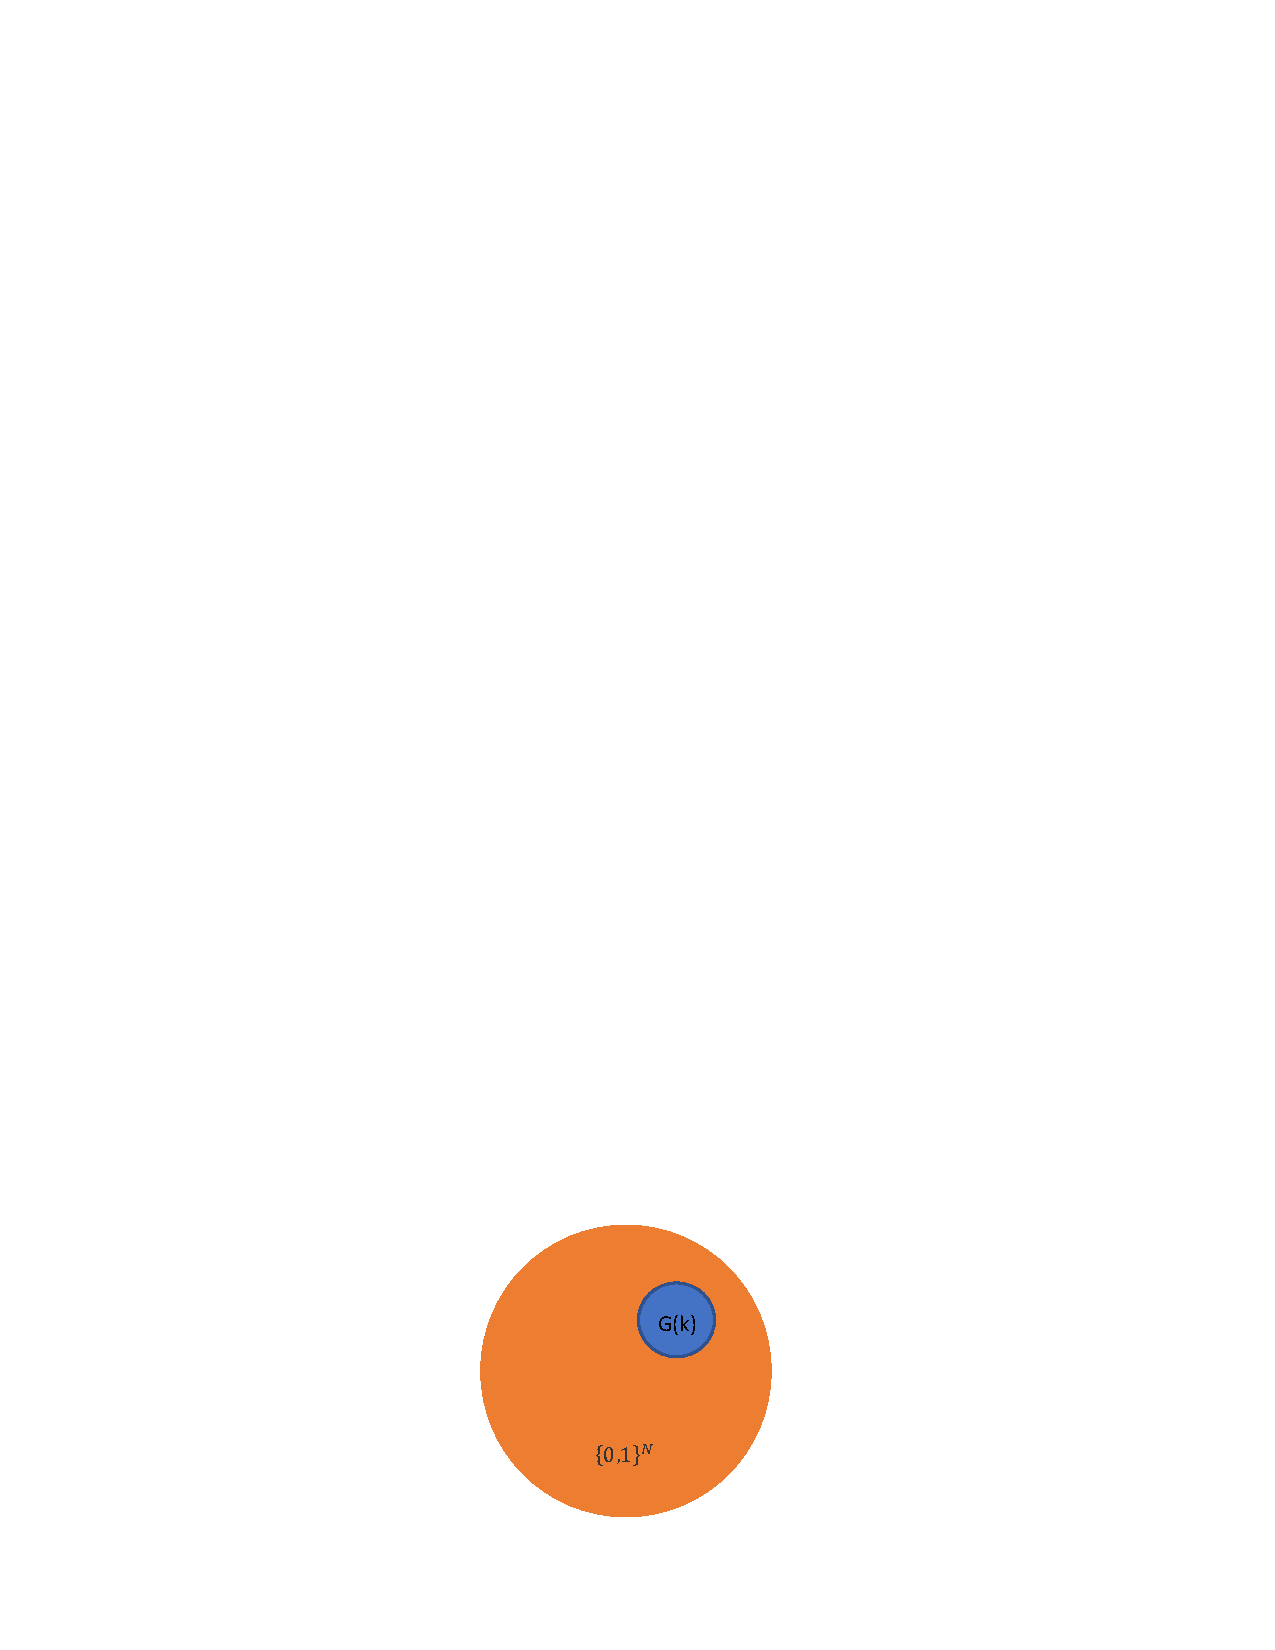
\includegraphics[scale=0.45]{fig1-27.pdf}\\
%\captionsetup{labelsep=colon}
\caption{}
\end{figure}

\paragraph{}
Remember that an arrow with R above it means choosing uniformly from the set script K. And then we output, basically, the output of the generator. And what we'd like to say. Is that this distribution of pseudo random strings is indistinguishable from a truly uniform distribution? In other words, if we just choose a truly uniform string in $\{0,1\}^N$ and simply output this string, we'd like to say that these two distributions are indistinguishable from one another. Now if you think about it, this sounds really surprising because if we draw a circle here of all possible strings in $\{0,1\}^N$, then the uniform distribution basically can output any of these strings with equal probability. That's the definition of the uniform distribution. However, for a pseudo-random distribution generated by this generator \textbf{G}, because the seed space is so small, the set of possible outputs is really small, it's tiny inside of, $\{0,1\}^N$. And this is really all that the generator can output. And yet, what we're arguing is that an adversary who looks at the output of the generator in this tiny set can't distinguish it from the output of the uniform distribution over the entire set. I think that's the property that we're actually shooting for. 
\paragraph{}
So, to understand how to define this concept of indistinguishability from random, we need the concept of a statistical test. So, let me define what a statistical test on $\{0,1\}^N$ is. I'm going to define these statistical tests by the letter A. And the statistical test is basically an algorithm that takes its inputs and N bit string, and simply outputs 0 or 1. Now I'll tell you that 0, we're going to think of it as though the statistical test said, the input you gave me is not random. And 1, we're going to think of it as saying that the input you gave me actually is random. All this statistical test does is it basically takes the input x that was given to it, the n bit string that was given to it, and decides whether it looks random or it doesn't look random. Let's look at a couple of examples.

\ex{}{
 The first example basically will use the fact that for a random string, the number of zeros is roughly equal to the number of ones in that string. In other words, the statistical test is going to say one. If and only if basically the number of zeros in the given string X minus the number of 1's in the given string X. These numbers are not too far apart. In other words, the difference between the number of 0's and the number of 1's. Let's just say is less than ten times square root of n. If the difference is less than ten times, the statistical test will say hey the string X looks random. If the difference happens to be much bigger than ten times square root of n, that starts to look suspicious and the test, hey the string you gave me does not look random.}
 \ex{}{
 Look at another similar example. In this string of, n bits. It counts a number of times that we see the pattern 00. Two consecutive zeros. Well for a random string. We will expect to see 0,0 as probability one fourth. And therefore, in a random string, we'll expect about $ \frac{n} {4}$ 00 s. And so, what the statistical test will do is it will say, well, if the number of 00 is roughly $ \frac{n} {4}$. In other words, the difference between the number and $ \frac{n} {4}$, is, say, less than ten square root of n, then we will say that X looks random. And if the gap is much bigger than $ \frac{n} {4}$, we'll say, hey, this string doesn't really look random. And then the statistical test will output zero}
 \paragraph{} 
So, here are two examples of statistical tests that basically, for random strings, they will output one with very high probability. But for strings that, you know, don't look random, for example, think of the all zero string. So, the all zero string, neither one of these tests will output, one. And in fact, the all zero string does not look random.
\paragraph{} 
Let's look at one more example of the statistical test just to kind of show you the, basically statistical test can pretty much do whatever they want. So, here's the third example. Let's say that statistical test output one if an only if I say the biggest blocks what we'll call this the Maximum Run of zero inside of the string x, this is basically the longest sequence of zero inside of the string x. In a random string you expect the longest sequence of zeros to be roughly of length $\log N $. So, we'll say if the longest sequence of zero happens to be less than ten times $\log N $ Then this test will say that X was random. But if, all of a sudden, we see a run of zeros that, say, is much bigger than ten $\log N $, then the statistical test will say, the string is not random. So, this is another crazy thing that the statistical test will do. By the way, you notice that if you give this test, the all one string. So, 11111. This test will also output 1. In other words, this test will think that the all 1 string is random. Even though it's not. Even though one string is not particularly random.
\paragraph{}
 Statistical tests don't have to get things right. They can do whatever they like. They can test, they can decide to output random or not. You know, zero or one, however they like. And similarly, there are many, many, many other statistical tests. There are literally hundreds of statistical tests that one can think of. And I can tell you that in the old days, basically, the way you would define that something looks random. As you would say, hey, here's a battery of statistical tests. And all of them said that this string looks random. Therefore, we say that this generator that generated the string is good generator. In other words, this definition, then, uses a fixed set of statistical tests, is actually not a good definition for security, but more generally, for crypto.
 \paragraph{}
 
 But before we talk about actually defining security, the next thing we talk about is how do we evaluate whether a statistical test is good or not? So, to do that, we define the concept of advantage. And so, let me define the advantage. So, here we have a generator that outputs N bit strings. And we have a statistical tests on N bit strings. And we define the advantage of this generator, as denoted by $Adv_{PRG}$, the advantage of the statistical test A relative to the generator G. I'll define it as follows, basically the difference between two quantities. 
\dfn{Advantage of statistical test $\mathcal{A}$ on PRG G:}{
\[
Adv_{PRG}\left(A,G\right)=\left|Pr\left(A\left(G\left(k\right)\right)=1\right)-Pr\left(A\left(r\right)=1\right)\right|\in[0,1]  k \xrightarrow{R}K, r\xrightarrow{R} {0,1}^N 
\]
}
The first quantity is basically, we ask how likely is this statistical test to output one. When we give it a pseudo random string just like here K is chosen uniformly from the C space, we ask how likely is the statistical test to output one when we give it a pseudo random output generated by the generator verses now, we ask how likely is the statistical test to output one when we give it a truly random string. So, here are is truly random in zero random one to the N. We look at the difference between these two quantities. Now you realize because these are differences of probabilities this advantage is always going to lie in the interval [0,1].
\paragraph{}
 So, let's think a little bit about what this advantage actually means. So, first of all if the advantage happens to be close to one. That means that somehow, the statistical test A behaves differently when we gave it pseudo-random inputs, when we gave it the output of the generator, for when we gave it truly random inputs, right? It somehow behaved differently. In one case, it output one with a certain probability. And in the other case, it output one with a very different probability. So, somehow, it was able to behave differently. And what they really mean is that the statistical test could distinguish the output of the generator from random. Okay, so in some sense we'll say that this statistical test broke the generator G because it was able to distinguish the output from random. However, if the advantage is close to zero Well what does that mean. That means that basically the statistical tests behave pretty much the same on pseudo random inputs. As it does on truly random inputs. And basically, there we would say that A could not distinguish the generator from random. 
 \paragraph{}
This sum gives you a little bit of intuition about why this concept of advantage is important. It basically tells us whether A was able to break the generator, namely distinguish it from random, or not able to break it. 
\qs{}{
So, let's look, first of all, at a very silly example. Suppose we have a statistical test A that simply ignores its inputs and always outputs zero. What do you think of the advantage of this statistical test relative to a generator G?}

\sol So, I hope you say the advantage is zero, let me just explain, why that's the case, well, if the statistical test, always outputs, zero, that means, pseudo random inputs, it will never output one, so, the probability that outputs one, is zero. Similarly, when we give a truly random input, it still will never output one, and, so, the probability that outputs one, is zero, and, so, zero minus zero is zero, so, its advantage is zero, so, basically, and, a statistical test that ignores its input, is not able to distinguish, truly random inputs, from a pseudo random input, obviously.
\paragraph{}
 Now let's look at a more interesting example. So, suppose we have a generator G that satisfies a funny property. It so happens that for two-thirds of the keys the first bit of the output of the generator happens to be 1. So, if I choose a random key, with probability two-thirds, the generator will output 1 as its first bit. So, that's the property of the generator that we're looking at. Now, let's look at the following statistical test. The statistical test basically says, if the most significant bit of the string you gave me is 1, I'm going to say one, meaning I think it's random. If the most significant bit of the stream you gave me is not 1, is 0, I'm going to say zero. Now my question to you is what is the advantage of this statistical test on the generator G?
 \paragraph{} 
Let me explain. Suppose we give the statistical tests pseudo random inputs. By definition of G, we know that with probability two-thirds, the first bits in the inputs will start with the bit one. But if it starts with a bit one, then the statistical test will output one. In other words, the probability that this statistical test outputs one is exactly two-thirds. Now let's look at the case of a random string. If I give you a random string, how likely is it that the most significant bits of the random string are one? Well, for a random string, that happens exactly half the time, and so in this case the statistical test will output one, with probability one-half. And so, the overall advantage is one-sixth, and one-sixth is actually a non-negligible number, that's actually a fairly large number, which basically means that this a was able to distinguish the output. We'll say that a breaks the generator G with advantage 1/6. Which means that this generator is no good, is broken.
\paragraph{}
 so now that we understand what statistical tests are, we can go ahead and define, what is a secure pseudo-random generator. So, basically, we say that, as generator G is secure, if essentially no efficient, statistical tests can distinguish its output from random. 

\dfn{secure PRG}{A PRG G is secure if the value $PRG_{adv}[A,G]$ is negligible for
all efficient adversaries $\mathcal{A}$.}

More precisely, what we'll say is that, basically for all efficient statistical tests A, if I look at the advantage. Of the statistical test A relative to G. This advantage basically is negligible. So, in other words, it's very close to zero, and as a result, this, statistical test was not able to distinguish the output from random, and that has to be true for all statistical tests. So, this is a very, very pretty and elegant definition, that says that a generator is secure, not only if a particular battery of statistical tests says that the output looks random, but, in fact, all efficient statistical tests will say the output looks random. 
\paragraph{}
One thing I'd like to point out is, that the restriction to efficient statistical tests is actually necessary. If we ask that all statistical tests, regardless of whether they're efficient or not be able to distinguish the output from random. Then in fact, that cannot be satisfied. So, in other words if we took out the requirements that the test be efficient. Then this definition would be unsatisfiable. And I'll leave this as a simple puzzle for you to think about. But basically, the fact is that restricting this definition into only efficient statistical tests is actually necessary for this to be satisfiable.
\paragraph{}
 So, now that we have a definition, the next question is can we actually construct a generator and then prove that it is in fact a secure PRG. In other words, prove that no efficient statistical test can distinguish its output from random. And it turns out that the answer is we actually can't. In fact, it's not known if there are any probably secure PRGs. Then I will just say very briefly the reason is that if you could prove that a particular generator is secure that would actually imply that P is not equal to NP. And I don't want to dwell on this. Because I don't want to assume that you guys know what P and NP are. But I'll tell you as a simple fact that in fact in P is equal to NP. Then it's very easy to show that there are no secure PRGs. And so, if you could prove to me that a particular PRG is secure, that would imply that P is not equal to NP. Again, I will leave this to you as a simple puzzle to think about. But even though we can't actually rigorously prove that a particular PRG is secure, we still have lots and lots and lots of heuristic candidates, and we even saw some of those in the previous segments. 
 \paragraph{}
Okay now that we understand what is a secure PRG. I want to talk a little bit about some applications and implications of this definition. And so, the first thing I want to show you is that in fact a secure PRG is necessarily unpredictable. In a previous segment, we talked about what it means for a generator to be unpredictable. And we said that, basically, what that means is that, given a prefix of the output generator, it's impossible to predict the next bit of the output. So we'd like to show that if a generator is secure, then necessarily, it means it's unpredictable. And so, the only way we're going to do that is using the contrapositive. That is, we're going to say that if you give me a generator that is predictable, then necessarily, it's insecure. In other words, necessarily, I can distinguish it from random. 
\thm{}{Let G be a PRG, defined over $\{0,1\}^N$. If G is secure, then G is unpredictable.}
\paragraph{}
\proof So, suppose you give me a predictor. In other words, suppose you give me an efficient algorithm, such that, in fact, if I give this algorithm the output of the generator, but I give it only the first I-bits of the outputs. It's able to predict the next bit of the output. In other words, given the first I-bit it's able to predict the I plus first bit. And it does that with a certain probability. So, let's say if we choose a random key k from the key space. Then, clearly, a dumb predictor would be able to predict the next bit with probability one-half, simply just guess the bits. However, this algorithm A is able to predict the next bit with probability half plus epsilon. So, it's bounded away from a half. And, in fact, we require that this by true for some non-negligible epsilon. So, for example, epsilon equal $ \frac{1}{1000}$ would already be a dangerous predictor, because it can predict the next bits, given a prefix, with non-negligible advantage.

\paragraph{}
therefor suppose we have such an algorithm. Let's see that we can use this algorithm to break our generator. In other words, to show that a generator is distinguishable from random and therefore, is insecure. So, what we'll do is we'll define a statistical test. So, let's define the statistical test B as follows. Basically, B, given a string, x, what it will do, is it will simply run algorithm A on the first I-bit of the string x that it was given. And, statistical test b is simply going to ask, was a successful in predicting the I-plus first bit of the string? If it was successful, then it's going to output one. And if it wasn't successful, then it's going to output zero.  This our statistical task. Let's put it in a box So, we can take it wherever we like. And we can run the statistical test on any N bit string that's given to us as inputs. So, now, let's look at what happens. Suppose we give the statistical test, a truly random string. So, a truly random string R. And we ask, what is the probability that the statistical test outputs one? Well, for a truly random string, the I+1 bit is totally independent of the first I-bits. So, whatever this algorithm is going to output is completely independent of what's, I+1 bit of the string R is. And so whatever A outputs the probability
is going to be equal to some random bit X I+1. Random independent bit X I+1, that probability is exactly $ \frac{1}{2}$. In other words, algorithm a simply has no information about what the bit X I+1 is, and so necessarily, the probability is able to predict X I+1 is exactly $ \frac{1}{2}$. On the other hand, let's look at what happens when we give our statistical tests a pseudo-random sequence. So, now we're going to run the statistical test on the output of the generator, and we ask how likely is it to output one. Well, by definition of A, we know that when we give it the first I bits of the output of the generator, it's able to predict the next bit with probability $ \frac{1}{2} + \epsilon$ . So, in this case our statistical test B will output one with probability greater than $ \frac{1}{2} + \epsilon$ and basically what this means, is if we look at the advantage of our statistical tests over the generator G it's basically, the difference between this quantity and that quantity. There's a difference between the two. You can see that it's clearly greater than an epsilon. So, what this means is that if algorithm A is able to predict the next bits with advantage epsilon, then algorithm B is able to distinguish the output of the generator with advantage epsilon. 
\paragraph{}
 So, if A is a good predictor, B is a good statistical test that break the generator. And as we said, the counter-positive of that is that if G is a secure generator, then there are no good statistical tests. And as a result, there are no predictors.  Which means that the generator is, as we said, unpredictable. So far, what we've seen is that if the generator is secure, necessarily, it's impossible to predict the I+1 bit, given first I bits. Now there's a very elegant and remarkable theorem by Yao back in 1982. They chose it, in fact the converse is also true. In other words, if I give you a generator that's unpredictable, so you cannot predict the I+1 bits from the first I bits, and that's true for all I. That generator, in fact, is secure. 

\thm{}{(Proven by Yao): Let G be a PRG, defined over $\{0,1\}^N$. If G is unpredictable, then G is secure.}

\paragraph{}
Let me state the theorem a little bit more precisely. So, here we have our generator that outputs n bit outputs. The theorem says the following, basically for all bit positions, it's impossible to predict I+1 bit of the output given the first I bit. And that's true for all I. In other words, again, the generator is unpredictable for all bit positions. Then, that, in fact, implies that the generator is a secure PRG. I want to paraphrase this in English, and so the way to kind of interpret this result is to say that consider these next bit predictors, that try to predict the I+1 bit given the first I bits. If they're not able to distinguish G from random, then, in fact, no statistical test is going to distinguish G from random. 
\paragraph{}
So, kind of next bit predictors are in some sense universal, predictors, when it comes to distinguishing things from random. This theorem, by the way, it's not too difficult to prove, but there's a very elegant idea behind its proof. I'm not going to do the proof here, but I encourage you to think about this as a puzzle, try to kind of try to prove this theorem yourself.
\qs{}{ Let me show you kind of one cute implication of this theorem. So, let me ask you the following question. Suppose I give you a generator and I tell you that given the last (n/2) bits of the output. It's easy to predict the first (n/2) bits of the outputs. So, given the last end bits, you can compute the first end bits. That's kind of the opposite of predictability. Predictability mean given the first bit; you can produce the next bits. Here, given the last bits, you can produce the first ones. And my question to you, does that mean that the generator is predictable?}
\paragraph{}
\sol This is kind of a simple application of Yao theorem. The answer is actually yes let me explain why how do we build this generator well, actually we're not going to build it I'm going to show you that the generator exists. Well because the last n/2 bits imply the first n/2 bits means is that g is not secure. Because just as we did before it's very easy to build a statistical test that will distinguish the output of G from uniform. So, G is not secure. But if G Is not secure, by Yao's Theorem, that means that G is predictable. So, in other words, there exists some I for which given the first I bits of the output, you can build the I+1 bits of the output. Okay, so even though I can't quite point to you a predicter, we know that a predicter must exist. So, that's a one cute simple application of Yao theorem.
 \paragraph{}
 Now before we end the part, I want to kind of, generalize a little bit of what we did. And introduce a little bit of important notation that's going to be useful actually throughout. So, we're going to generalize the concept of indistinguishability from uniform, to indistinguishability of two general distributions. So, suppose I give you distributions $p_1$ and $p_2$, and we ask, can these two distributions be distinguished? And so, we'll say that the distributions are computationally indistinguishable, and we'll denote this by $p_1\approx_p p_2$. This means that, in polynomial time, $P_1$ cannot be distinguished from $P_2$. And we'll say that they're indistinguishable, basically, just as before if for all, efficient, statistical tests A it so happens that if I sample from the distribution $P_1$, and I give the output to A, versus if I sample from the distribution $P_2$, and I give the sample to A, Then, basically A behaves the same in both cases. In another-wards the difference between these two probabilities is negligible. And this has to be true for all statistical tests. For all efficient statistical tests. 
\dfn{Computationally indistinguishable distributions}{
\[ |Pr(A(x)=1)-Pr(A(y=1)|<\epsilon\quad x \xrightarrow{R}p_1,\; y\xrightarrow{R}p_2
\]
}

\paragraph{}
So, if this is the case then we say that, well A couldn't distinguish its advantage in distinguishing two distributions is negligible and if that's true for all efficient statistical tests then we say that the distributions are basically computationally indistinguishable, because an efficient algorithm cannot distinguish them. And just to show you how useful this notation is, basically using this notation the definition of security for PRG just says. That if I give you a pseudo-random distribution. In other words, I choose K at random, and that outputs a G of K. That distribution is computationally indistinguishable from the uniform distribution. So, you can see this, this very simple notation captures the whole definition of pseudo-random generators. Okay, so we're going to make use of this notation. In the next segment, when we define, what does it mean for a cipher to be secure.

\subsection{Semantic Security}
\paragraph{}
My goal for the next few part in this chapter is to show you that if we use a secure PRG we'll get a secure stream cipher. The first thing we have to do is define, what does it mean for a stream safer to be secure? Whenever we define security, we always define it in terms of what can the attacker do? And what is the attacker trying to do? In the context of stream ciphers, remember these are only used with a one-time key, and as a result the most the attacker is ever going to see is just one cipher text encrypted using the key that we're using. And so, we're going to limit the attacker’s ability to basically obtain just one cipher text. And in fact, later on we're going to allow the attacker to do much, much more, but for now we're just going to give him one cipher text. And we wanted to find, what does it mean for the cipher to be secure? 
\paragraph{}
The first definition that comes to mind is basically to say, well maybe we want to require that the attacker can't actually recover the secret key. So given ciphertext you shouldn't be able to recover the secret key. But that's a terrible definition because think about the following brilliant cipher but the way we encrypt the message using a key K is basically we just output the message. Okay this is a brilliant cipher of course it doesn't do anything given a message just output a message as the cipher text. This is not a particularly good encryption scheme; however, given the cipher text, mainly the message the poor attacker cannot recover the key because he doesn't know what the key is. So as a result, this cipher which clearly is insecure, would be considered secure under this requirement for security. 
\paragraph{}
Attempt one: attacker cannot find the key. Example showing is it not a good definition: E(k,m)=m
\paragraph{}
So, this definition will be no good. It's recovering the secret key is the wrong way to define security. The next thing we can kind of attempt is basically just say, well maybe the attacker doesn't care about the secret key, what he really cares about are the plain text. So maybe it should be hard for the attacker to recover the entire plain text. But even that doesn't work because let's think about the following encryption scheme. Suppose what this encryption scheme does is it takes two messages, so I'm going to use two lines to denote concatenation of two messages $m_0||m_1$ means concatenate $m_0$ and $m_1$. And imagine what the scheme does, it really outputs $m_0$ in the clear and concatenate to that the encryption of $m_1$. Perhaps even using the One-time Pad . And so here the attacker is going to be given one cipher text. And his goal would be to recover the entire plain texts. But the poor attacker can't do that because here maybe we've encrypted $m_1$ using the One-time Pad so the attacker can't actually recover $m_1$ because we know the One-time Pad is secure given just one cipher text. 
\paragraph{}
Attempt two: attacker cannot find the key. Example showing is it not a good definition: $E(k,m_0||m_1)=m_0||m_1\oplus k$
\paragraph{}
This construction would satisfy the definition but unfortunately clearly this is not a secure encryption scheme because we just leaked half of the plain text. $m_0$ is completely available to the attacker so even though he can't recover all of the plain text he might be able to recover most of the plain text, and that's clearly unsecured. So of course, we already know the solution to this and we talked about Shannon definition of security perfect secrecy where Shannon's idea was that in fact when the attacker intercepts a ciphertext he should learn absolutely no information about the plain texts. He shouldn't even learn one bit about the plain text or even he shouldn't learn, he shouldn't even be able to predict a little bit about a bit of the plain text. Absolutely no information about the plain text. 
\paragraph{}
So let's recall very briefly Shannon's concept of perfect secrecy. Basically, we said that given a cipher, we said the cipher has perfect secrecy if given two messages of the same length it so happens that if we pick a random key and we look into distribution of cipher texts we encrypt $m_0$ we get exactly the same distribution as when we encrypt $m_1$. The intuition here was that if the adversary observes the cipher texts then he doesn't know whether it came from the distribution the result of encrypting $m_0$ or it came from the distribution as the result of encrypting $m_1$. And as a result, he can't tell whether we encrypted $m_0$ or $m_1$. And that's true for all messages of the same length and as a result a poor attacker doesn't really know what message was encrypted. 
\paragraph{}
Of course, we already said that this definition is too strong in the sense that it requires really long keys if cipher has short keys can't possibly satisfy this definition in a particular stream ciphers can satisfy this definition. So let's try to weaken the definition a little bit and let's think to the previous part, and we can say that instead of requiring the two distributions to be absolutely identical, what we can require is that two distributions just be computationally indistinguishable. In other words, a poor, efficient attacker cannot distinguish the two distributions even though the distributions might be very, very different. That just given a sample for one distribution and a sample for another distribution the attacker can't tell which distribution he was given a sample from.
\paragraph{}
 It turns out this definition is actually almost right, but it's still a little too strong, that still cannot be satisfied, so we have to add one more constraint, and that is that instead of saying that this definition should have hold for all $m_0$ and $m_1$. It is to hold for only pairs $m_0$ $m_1$ that the attackers could actually exhibit. This actually leads us to the definition of semantic security. This is semantic security for one-time key in other words when the attacker is only given one cipher text.
 
 \begin{figure}[H]
\centering
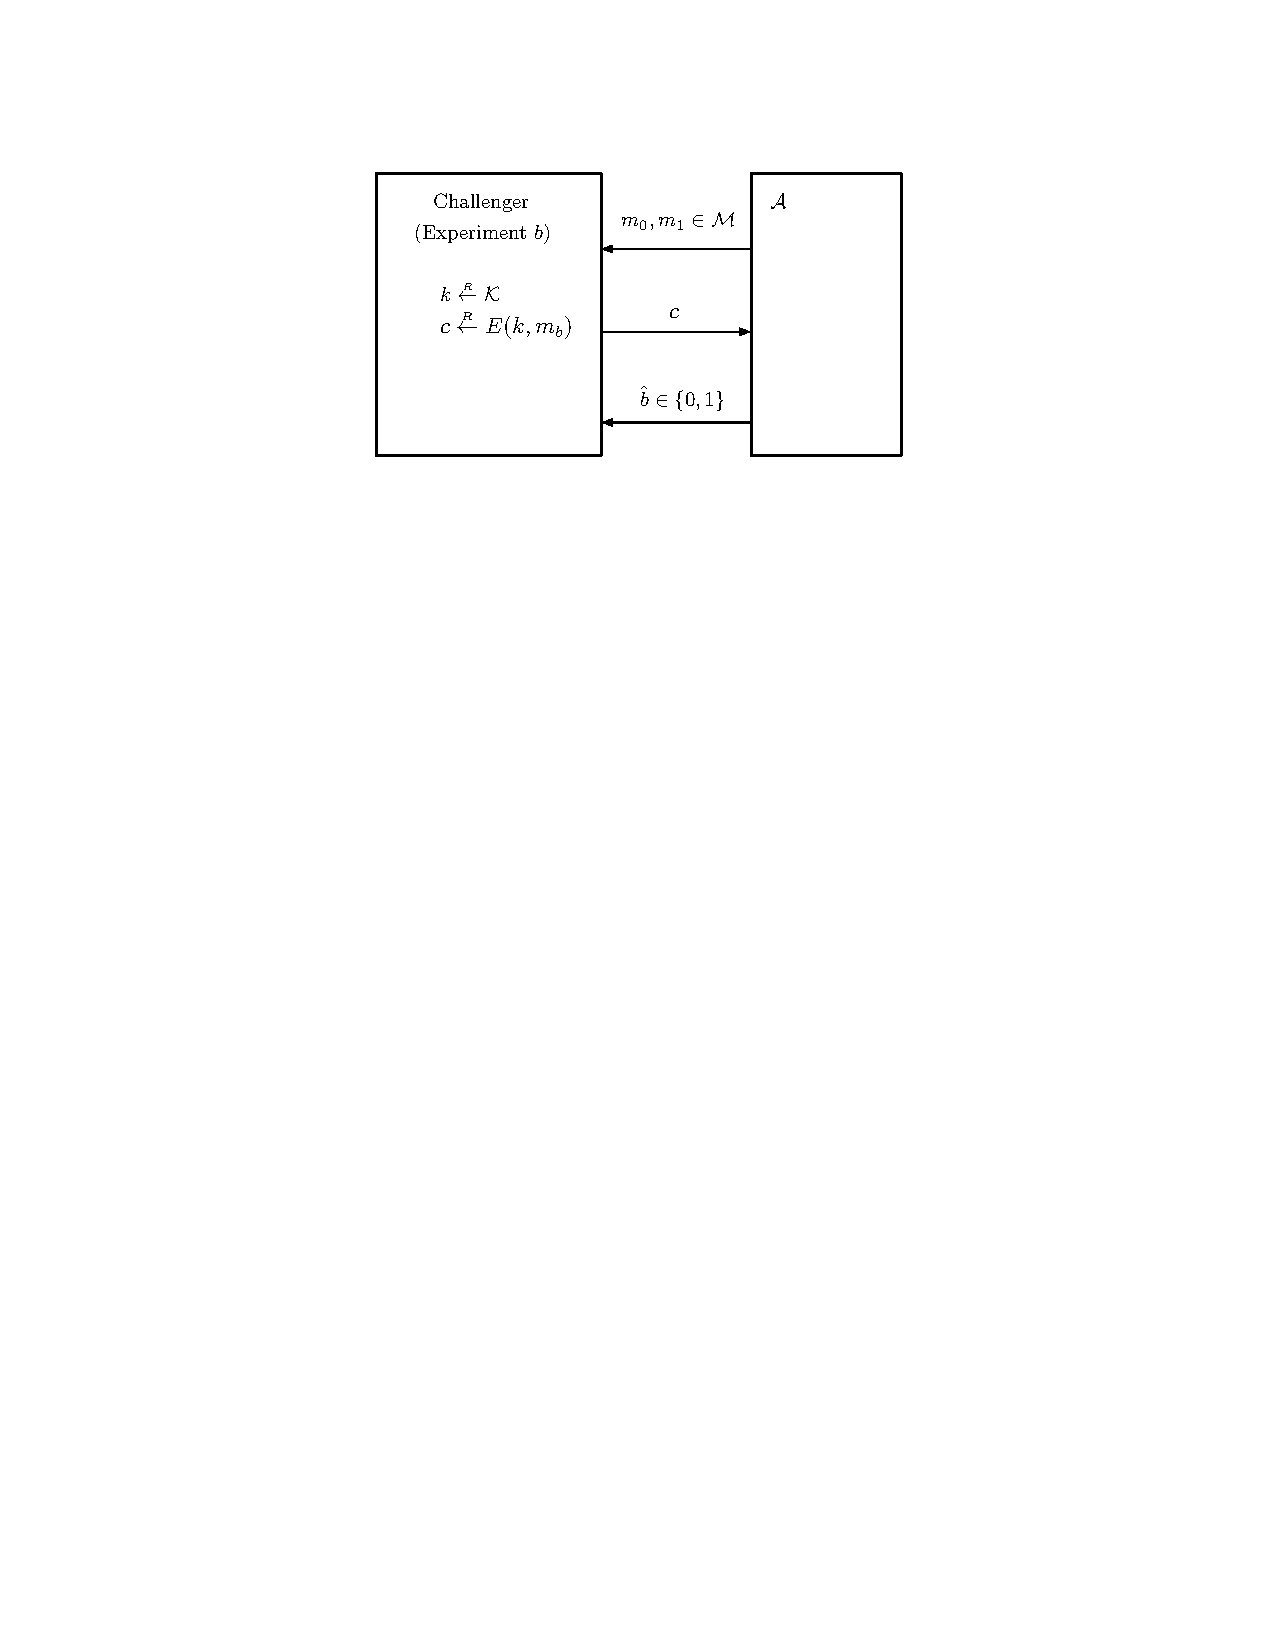
\includegraphics[scale=0.65]{fig1-28.pdf}\\
\captionsetup{labelsep=colon}
\caption{Semantic Security Game}
\end{figure}

  The way we define semantic security is by defining two experiments, experiment 0 and experiment 1. And more generally we will think of these as $ e^b $, where b can be zero or one. So the way the experiment is defined is as follows, we have an adversary that's trying to break the system. An adversary A, that's the analog of statistical tests in the world of pseudo random generators. Really, we have two challengers, but the challengers are so similar that we can just describe them as a single challenger that in one case takes his input bit set to zero, and the other case takes his input bit set to one. And let me show you what these challengers do. The first thing the challenger is going to do is it's going to pick a random key and then the adversary basically is going to output two messages $m_0$ and $m_1$. This is an explicit pair of messages that the attacker wants to be challenged on and as usual we're not trying to hide the length of the messages; we require that the messages be equal length. And then the challenger basically will output either the encryption of $m_0$ or the encryption of $m_1$, so in experiment 0 the challenger will output the encryption of $m_0$. In experiment 1 the challenger will output the encryption of $m_1$. Okay so that the difference between the two experiments. And then the adversary is trying to guess basically whether he was given the encryption of $m_0$ or given the encryption of $m_1$.
  \paragraph{} 
Let's define the events $W_b$ to be the events that an experiment b (0 or 1) the adversary outputs one. So that is just an event that basically in experiment 0, $W_0$ means that the adversary output one and in experiment one $W_1$ means the adversary output one. And now we can define the advantage of this adversary, to say that this is called the semantic security advantage of the adversary A against the scheme E, to be the difference of the probability of these two events.

\dfn{Semantic Security game}{For a given cipher $E = (E,D)$, defined over $(\mathcal{K},\mathcal{M},\mathcal{C})$,
and for a given adversary $\mathcal{A}$, we define two experiments, Experiment 0 and Experiment 1. For
$b \in \{0, 1\}$, we define:\\
\textbf{Experiment} $b$
\begin{enumerate}
\item The adversary computes $(m_0,m_1) \in M$, of the same length, and sends them to the challenger.
\item The challenger computes $k \xrightarrow{R} K, c \xrightarrow{r} E(k,m_b)$, and sends c to the adversary.
\item The adversary outputs a bit $\hat{b}\in \{0,1\}$.
\end{enumerate}
For $b \in \{0, 1\}$, let $W_b$ be the event that $\mathcal{A}$ outputs 1 in Experiment b.
We define $\mathcal{A}$'s semantic
security advantage with respect to E as
\[ Adv_{SS}[\mathcal{A},\mathcal{E}] :=|Pr[W_0] - Pr[W1]| \]
}
\paragraph{}
In other words, we are looking at whether the adversary behaves differently when he was given the encryption of $m_0$ from when he was given the encryption of $m_1$. I want to make sure this is clear so I'm going to say it one more time. So, in experiment zero he was given the encryption of $m_0$ and in experiment one he was given the encryption of $m_1$. Now we're just interested in whether the adversary outputs 1 or not, in these experiments. If in both experiments the adversary output 1 with the same probability that means the adversary wasn't able to distinguish the two experiments. Experiments zero basically looks to the adversary the same as experiment one because in both cases output one with the same probability. However, if the adversary is able to output 1 in one experiment with significantly different probability than in the other experiment, then the adversary was actually able to distinguish the two experiments. 
\paragraph{}
To say this more formally, essentially again because the advantage is the difference of two probabilities it’s a number between zero and one. If the advantage is close to zero, that means that the adversary was not able to distinguish experiment zero from experiment one. However if the advantage is close to one, that means the adversary was very well able to distinguish experiment zero from experiment one and that really means that he was able to distinguish an encryption of $m_0$ from an encryption of $m_1$, That's out definition. Actually, that is just the definition of the advantage and the definition is just what you would expect basically we'll say that a symmetric encryption scheme is semantically secure if "For all efficient adversaries the advantage is negligible." 
\paragraph{}
In other words, no efficient adversary can distinguish the encryption of $m_0$ from the encryption of $m_1$ and basically this is what it says repeatedly that for these two messages that the adversary was able to exhibit he wasn't able to distinguish these two distributions. Now I want to show you this, this is actually a very elegant definition. It might not seem so right away, but I want to show you some implications of this definition and you'll see exactly why the definition is the way it is.

\dfn{Semantically Secure cipher}{An encryption scheme is semantically secure if for all “efficient” adversaries, the advantage is negligible, meaning for all explicit $m_0$ and $m_1$, $E(k,m_0)\approx E(k,m_1)$}

\paragraph{} Let's look at some examples. So the first example is suppose we have a broken encryption scheme, in other words suppose we have an adversary A that somehow given the cipher text he is always able to deduce the least significant bit of the plain text. Okay so given the encryption of $m_0$, this adversary is able to deduce the least significant bit of $m_0$. So that is a terrible encryption scheme because it basically leaks the least significant bit of the plain text just given the cipher text. I want to show you that this scheme is therefore semantically secure so that kind of shows that if a system is semantically secure than there is no attacker of this type.

 \begin{figure}[H]
\centering
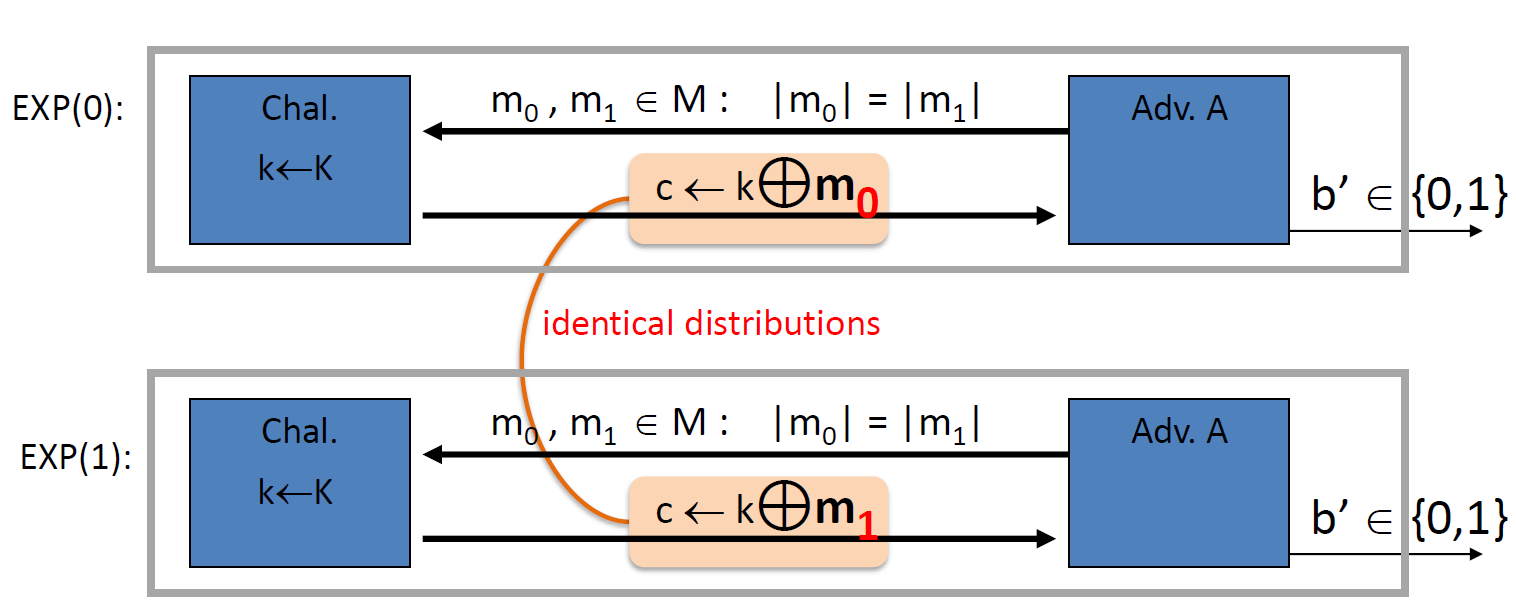
\includegraphics[scale=0.45]{fig1-28.png}\\
%\captionsetup{labelsep=colon}
\caption{}
\end{figure}


\paragraph{}Let's see why is the system not semantically secure well so what we are going to do is we're going to basically use our adversary who is able to learn our most insignificant bits, we're going to use him to break semantic security so we're going to use him to distinguish experiment zero from experiment one Okay so here is what we are going to do. We are algorithm B, we are going to be algorithm B and this algorithm B is going to use algorithm A in its belly. The first thing that is going to happen is of course the challenger is going to choose a random key. The first thing that is going to happen is that we need to output two messages. The messages that we are going to output basically are going to have different significant bits. One message is going to end with zero and one message is going to end with one. Now what is the challenger going to do? The challenger is going to give us the encryption of either $m_0$ or $m_1$, depending on whether in experiment 0 or in experiment 1. And then we just forward this cipher text to the adversary okay so the adversary A. Now what is the property of adversary A? Given the cipher text, adversary A can tell us what the least significant bits of the plain text is. In other words, the adversary is going to output the least significant bits of $m_0$ or $m_1$ but low and behold that's basically the bit B. And then we're just going to output that as our guess so call this thing B prime. Now this describes the semantic security adversary. And now you tell me what is the semantic security advantage of this adversary?
\paragraph{} 
Well so let's see. In experiment zero, what is the probability that adversary B outputs one? Well in experiment zero it is always given the encryption of $m_0$ and therefore adversary A is always output the least significant bit of $m_0$ which always happens to be zero. In experiment zero, B always outputs zero. So the probability that outputs one is zero. However, in experiment one, we're given the encryption of $m_1$. So how likely is adversary B to output one in experiment one well it always outputs one, again by the properties of algorithm A and therefore the advantage basically is one. So this is a huge advantage, it's as big as it's going to get. Which means that this adversary completely broke the system. So we consider, so under semantic security basically just deducing the least significant bits is enough to completely break the system under a semantic security definition. 
\paragraph{}
Now the interesting thing here of course is that this is not just about the least significant bit, in fact of the message for example the most significant bit, you know bit number seven Maybe the XOR of all the bits in the message and so on and so forth any kind of information, any bit about the plain text they can be learned basically would mean that the system is not semantically secure. Basically all the adversary would have to do would be to come up with two messages $m_0$ and $m_1$ such that under one thing that they learned it's the value zero and then the other thing, the value, is one. So for example if A was able to learn the XOR bits of the message then $m_0$ and $m_1$ would just have different XOR for all the bits of their messages and then this adversary A would also be sufficient to break semantic security. So, basically for cipher is semantically secure then no bit of information is revealed to an efficient adversary. So this is exactly a concept of perfect secrecy only applied to just efficient adversaries rather than all adversaries.
\paragraph{}
The next thing I want to show you is that in fact the one-time pad in fact is semantically secure, they better be semantically secure because it's in fact, it's more than that it's perfectly secure. Let's see why that's true, intuitively.

 \begin{figure}[H]
\centering
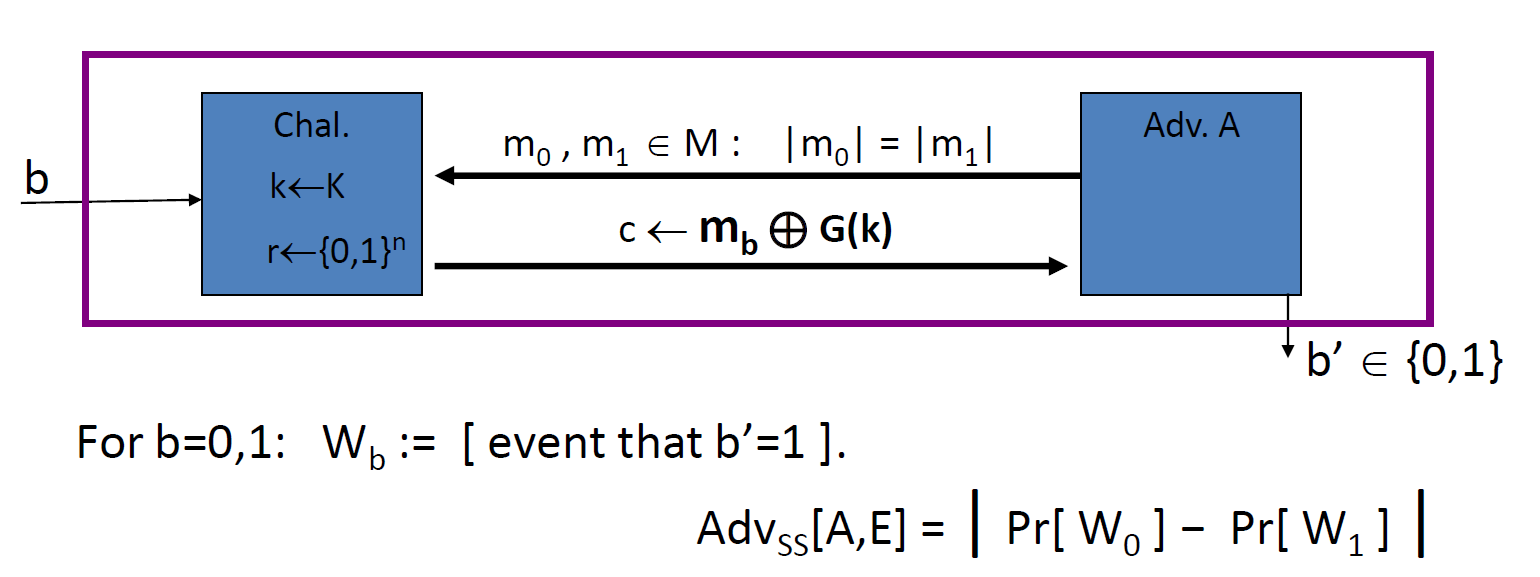
\includegraphics[scale=0.45]{fig1-29.png}\\
%\captionsetup{labelsep=colon}
\caption{}
\end{figure}

\paragraph{}
Well so again it's one of these experiments, so suppose we have an adversary that claims to break semantic security of the one-time pad. The first the adversary is going to do is he's going to output two messages $m_0$ and $m_1$ of the same length. Now what does he get back as a challenge? As a challenge, he gets either the encryption of $m_0$ or the encryption of $m_1$ under the one-time pad. And he's trying to distinguish between those two possible cipher texts that he gets, right? In experiment zero, he gets the encryption of $m_0$ and in experiment one, he gets the encryption of $m_1$. Well so let me ask you, so what is the advantage of adversary A against the one-time patent?  I remember that the property of the ones I had is that, that $k\oplus m_0$ is distributed identically to $k\oplus m_1$. In other words, these distributions are absolutely identical. This is a property of XOR. If we XOR the random pad K with anything, either $m_0$ or $m_1$, we get a uniform distribution. 
\paragraph{}
So, in both cases, algorithm A is given as in input exactly the same distribution. Maybe the uniform distribution on ciphertexts. Therefore, it's going to behave exactly the same in both cases because it was given the exact distribution as input. And as a result, its advantage is zero, which means that the onetime pad is semantically secure. Now the interesting thing here is not only is it semantically secure, it's semantically secure for all adversaries. We don't even have to restrict the adversaries to be efficient. No adversary, doesn't matter how smart you are, no adversary will be able to distinguish $k\oplus m_0$ from $k\oplus m_1$ because the two distributions are identical. The one-time pad is semantically secure. That completes our definition of semantic security so the next thing we're going to do is prove to the secure PRG, in fact implies that the stream cipher is semantically secure.

\subsection{Stream Ciphers are semantically secure}

\paragraph{}So now that we understand what a secure PRG is, and we understand what semantic security means, we can actually argue that a stream cipher with a secure PRG is, in fact, a semantically secure. So that's our goal for this, segment. It's a fairly straightforward proof, and we'll see how it goes. So the theorem we want to prove is that, basically, given a generator G that happens to be a secure, pseudo-random generator. In fact, the stream cipher that's derived from this generator is going to be semantically secure.

\thm{}{If we have a secure PRG, using the PRG for a stream cipher results in a semantically secure cipher.}

\proof   I want to emphasize. That there was no hope of proving a theorem like this for perfect secrecy, for Shannon’s concept of perfect secrecy. Because we know that a stream cipher cannot be perfectly secure because it has short keys. And perfect secrecy requires the keys to be as long as the message. So this is really kind of the first example the we see where we're able to prove that a cipher with short keys has security. The concept of security is semantic security. And this is a very useful concept. And in fact, you know, we'll be using semantic security many, many times throughout the lecture.
\paragraph{}How do we prove a theory like this? What we're actually going to be doing, is we're going to be proving the contrapositive. What we're going to show is the following. 
\[ Adv_{SS}(A,E)\leq 2\times Adv_{PRG}(A,G)\]

\paragraph{}
Suppose you give me a semantic security adversary A. What we'll do is we'll build a PRG adversary B to satisfy this inequality here. Now why is this inequality useful? We know that if B is an efficient adversary. Then we know that since G is a secure generator, we know that this advantage is negligible, right? A secure generator has a negligible advantage against any efficient statistical test. So the right hand side, basically, is going to be negligible. But because the right hand side is negligible, we can deduce that the left hand side is negligible. And therefore, the adversary that you looked at actually has negligible advantage in attacking the stream cipher E.So this is how this will work. All we have to do is given an adversary A we're going to build an adversary B. We know that B has negligible advantage against generator but that implies that A has negligible advantage against the stream cipher.
\paragraph{}
Let A be a semantic security adversary against the stream cipher. So, let me remind you what that means. Basically, there's a challenger. The challenger starts off by choosing the key K. And then the adversary is going to output two messages, two equal-length messages. And he's going to receive the encryption of $m_0$ or $m_1$ and outputs $b=1$ .  That's what a semantic security adversary is going to do. So now we're going to start playing games with this adversary. And that's how we're going to prove our lemma. So the first thing we're going to do is we're going to make the challenger. Also choose a random R. So, well you know the adversary doesn't really care what the challenger does internally. The challenger never uses R, so this doesn't affect the adversary's advantage at all. The adversary just doesn't care that the challenger also picks R.

 \begin{figure}[H]
\centering
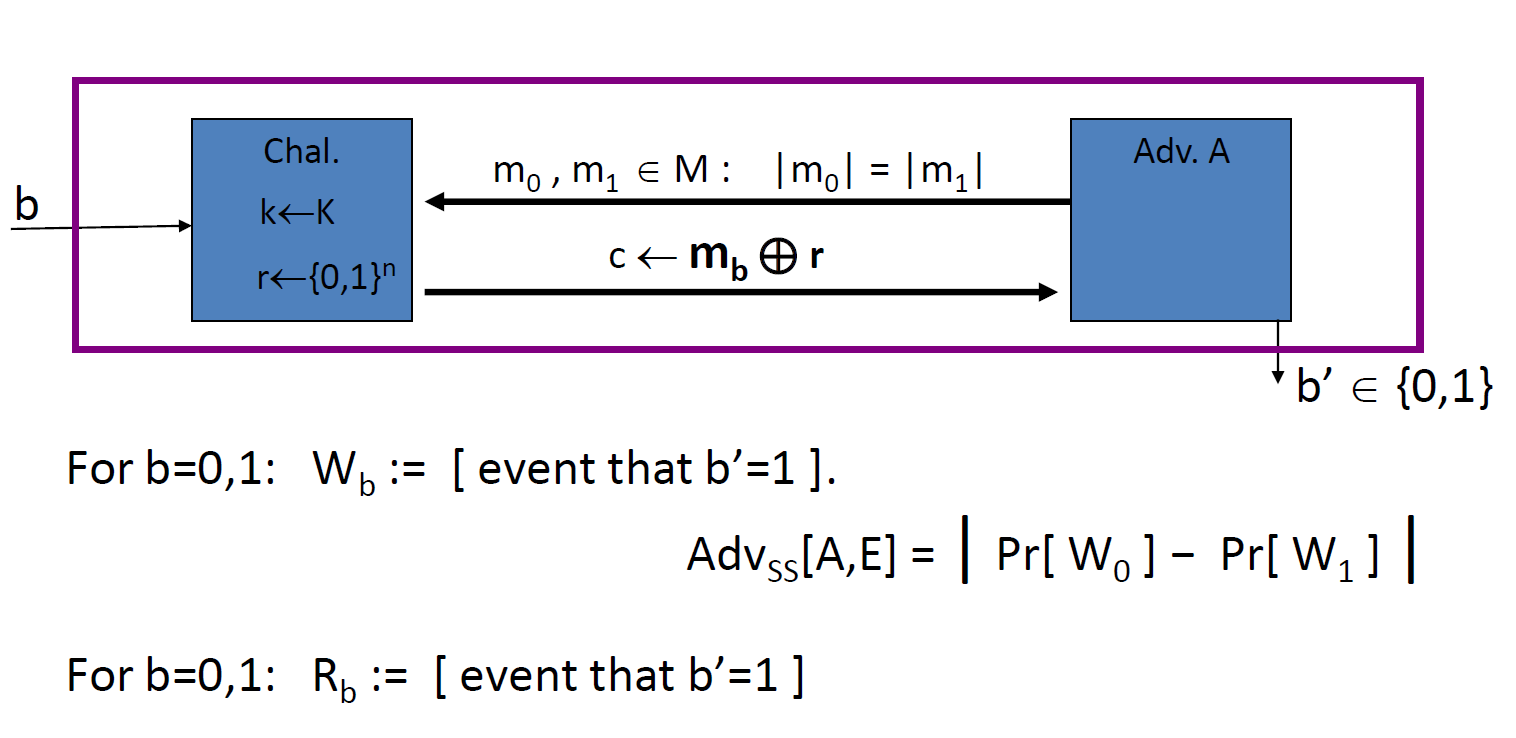
\includegraphics[scale=0.45]{fig1-30.png}\\
%\captionsetup{labelsep=colon}
\caption{}
\end{figure}

\paragraph{}
But now comes the trick. What we're going to do is we're going to, instead of encrypting using G(k). We're going to encrypt using r. You can see basically what we're doing here. We're changing the challenger so now the challenge cipher text is encrypted using a truly random pad. As opposed to just pseudo random pad G(k). Now, the property of the pseudo-random generator is that its output is indistinguishable from truly random. 

\paragraph{}
So, because the PRG is secure, the adversary can't tell that we made this change. The adversary can't tell that we switched from a pseudo-random string to a truly random string. Again, because the generator is secure. Well, but now look at the game that we ended up with. So the adversary's advantage couldn't have changed by much, because he can't tell the difference. But now look at the game that we ended up with. Now this game is truly a one-time pad game. This a semantic security game against the one-time pad. Because now the adversary is getting a one-time pad encryption of $m_0$ or $m_1$ But in the one-time pad we know that the adversaries advantage is zero, because you can't beat the one time pad. The one-time pad is unconditionally secure. And as a result, because of this. Essentially because the adversary couldn't have told the difference when we moved from pseudo random to random. But he couldn't win the random game. That also means that he couldn't win the pseudo random game. And as a result, the stream cipher, the original stream cipher must be secure.
\paragraph{}
 So that's the intuition for how the proof is going to go. But I want to do it rigorously once. From now on, we're just going to argue by playing games with our challenger. And, we won't be doing things as formal as I'm going to do next. But I want to do formally and precisely once, just so that you see how these proofs actually work. Okay, so I'm going to have to introduce some notation. And I'll do the usual notation, basically. If the original semantics are here at the beginning, when we're actually using a pseudo-random pad, I'm going to use $W_0$ and W1 to denote the event that the adversary outputs one, when it gets the encryption of $m_0$, or gets the encryption of $m_1$, respectively. So W0 corresponds to outputting 1 when receiving the encryption of $m_0$. And $W_1$ corresponds to outputting 1 when receiving the encryption of $m_1$. So that's the standard definition of semantic security. 
 \paragraph{}
Now once we flip to the random pad. I'm going to use R0 and $R_1$ to denote the event that the adversary outputs 1 when receiving the one-type pad encryption of $m_0$ or the one-time pad encryption of $m_1$. So we have four events, $W_0$, $W_1$ from the original semantic security game, and $R_0$ and $R_1$ from the semantic security game once we switch over to the one-time pad. So now let's look at relations between these variables. So first of all, $R_0$ and $R_1$ are basically events from a semantic security game against a one-time pad. So the difference between these probabilities is that, as we said, basically the advantage of algorithm A, of adversary A, against the one-time pad. Which we know is zero.  So that's great. So that basically means that probability of, of $R_0$ is equal to the probability of $R_1$. So now, let's put these events on a line, on a line segment between zero and one. 

 \begin{figure}[H]
\centering
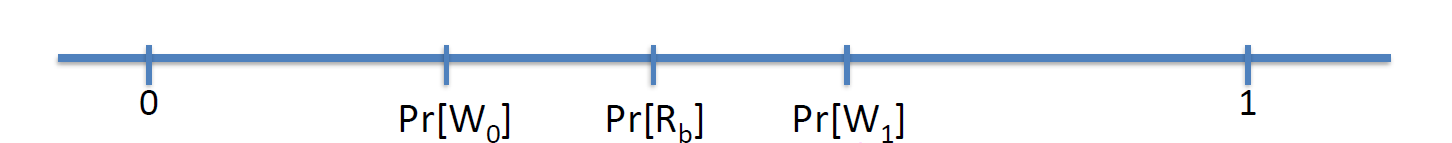
\includegraphics[scale=0.45]{fig1-31.png}\\
%\captionsetup{labelsep=colon}
\caption{}
\end{figure}

\paragraph{}
So here are the events. $W_0$ and $W_1$ are the events we're interested in. We want to show that these two are close.  And the way we're going to do it is basically by showing, oh and I should say, here is probability $R_0$ and $R_1$, it says they're both same, I just put them in the same place. What we're going to do is we're going to show that both $W_0$ and $W_1$ are actually close to the probability of $R_b$ and as a result they must be close to one another. Okay, so the way we do that is using a second claim, so now we're interested in the distance between probability of Wb and the probability of $R_b$. So we'll prove the claim in a second. Let me just state the claim.

\clm{}{}{$Pr(r_0=1)=Pr(r_1=1)$}
\clm{}{}{Adversary B exists such that $|Pr(W_b)-Pr(r_b)|=Adv_{PRG}(B,G)$}

\paragraph{} The claim says that there exists an adversary B. Such that the difference of these two probabilities is basically the advantage of B against the generator G and this is for both b's. So given these two claims, the theorem is done because basically what do we know. We know this distance is less than the advantage of B against G. That's from claim two and similarly, this distance actually is even equal to, I'm not going to say less but is equal to the advantage. Of B against G, and as a result you can see that the distance between $W_0$ and $W_1$ is basically almost twice the advantage of B against G. That's basically the thing that we are trying to prove. 
 \begin{figure}[H]
\centering
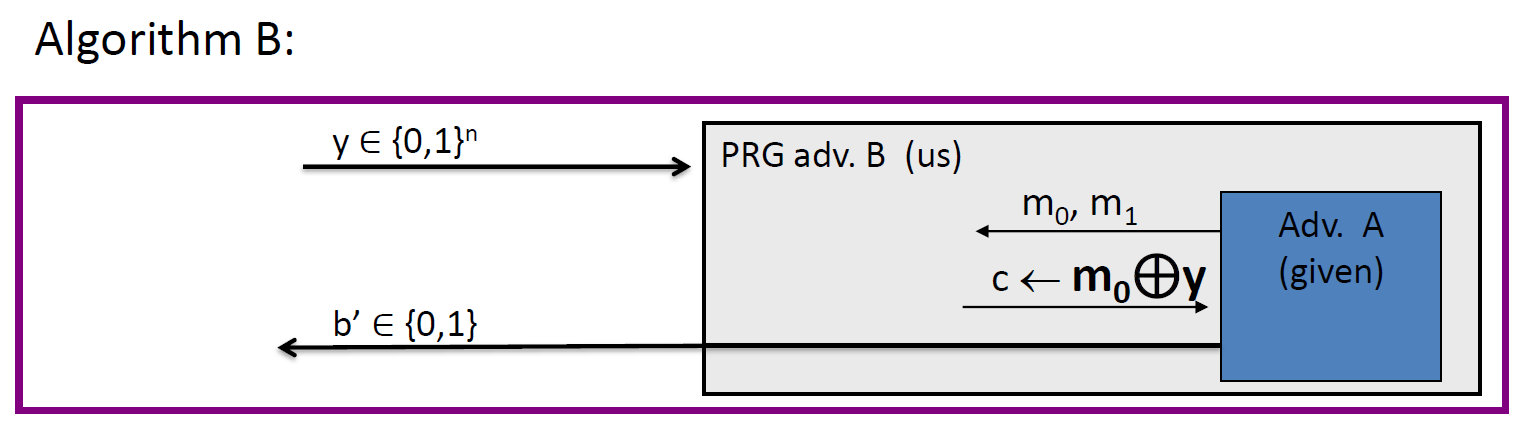
\includegraphics[scale=0.45]{fig1-32.png}\\
%\captionsetup{labelsep=colon}
\caption{}
\end{figure}

\paragraph{}
The only thing that remains is just proving this claim two and if you think about what claim two says, it basically captures the question of what happens in experiment zero what happens when we replace the pseudo random pad G(k), by truly random pad R. In the first game in experiment zero say we're using the pseudo random pad and in the second game in experiment zero we are using a truly random pad and we are asking can the adversary tell the difference between these two and we want to argue that he cannot because the generator is secure.
\paragraph{}
 So here's what we are going to do. So let's prove claim two. We are going to argue that in fact there is a PRG adversary B that has exactly the difference of the two probabilities as it's advantage. Okay and the point is since this is negligible that is negligible. And that's basically what we wanted to prove. 
 \paragraph{}
 Okay, so let's look at the statistical test b. So, what, our statistical test b is going to use adversary A in his belly, so we get to build statistical test b however we want. As we said, it's going to use adversary A inside of it, for its operation, and it's a regular statistical test, so it takes an n-bit string as inputs, and it's supposed to output, you know, random or non-random, zero or one. So let's see. So it's, first thing it's going to do, is it's going to run adversary A, and adversary A is going to output two messages, $m_0$ and $m_1$. And then, what adversary b's going to do, is basically going to respond. With $m_0$ XOR or the string that it was given as inputs. Alright? That's the statistical lesson, then. Whenever A outputs, it's going to output, its output. And now let's look at its advantage. What can we say about the advantage of this statistical test against the generator? Well, so by definition, it's the probability that, if you choose a truly random string, that b outputs 1 minus the probability, when we choose a pseudo random string, b outputs 1. 
 \paragraph{}
Okay, but let's think about what this is. Well, by the definition that's exactly if you think about what's going on here, that's this is exactly the probability $R_0$ right? Because this game that we are playing with the adversary here is basically he helped us $m_0$ and $m_1$ right here he helped add $m_0$ and $m_1$ and he got the encryption of $m_0$ under truly one-time pad. Here let me write this a little better. That's the basic level probability of $R_0$. Now, what can we say about the next expression, well what can we say about when B is given a pseudo random string Y as input. Well in that case, this is exactly experiment zero and true stream cipher game because now we're computing $m\oplus m_0\oplus G\left(k\right)$. This is exactly $W_0$. Okay, that's exactly what we have to prove. So it's kind of a trivial proof. Okay, so that completes the proof of claim two. And again, just to make sure this is all clear, once we have claim two, we know that $W_0$ must be close to W1, and that's the theorem. That's what we have to prove. Now we've established that a stream cipher is in fact semantically secure, assuming that the PRG is secure.
\[Adv_{PRG}(B,g)=|Pr(B(r)=1)-Pr(B(G(k)=1)|=|Pr(r_0)-Pr(W_0)|
\]


\chapter{Block Ciphers}

\section{Block Ciphers 1: Overview}
\subsection{What are Block Ciphers?}
Now that we understand stream ciphers, we're going to move on and talk about a more powerful primitive called a block cipher. So a block cipher is made up of two algorithms, \textbf{E} and \textbf{D}. These are encryption and decryption algorithms. And both of these algorithms take, as input, a key \textbf{K}. Now, the point of a block cipher is that it takes an N bit plain text as input, and it outputs exactly the same number of bits as outputs. So it maps N bits on inputs to exactly N bits of outputs.
\paragraph{} \ex{Important Block Cipher examples}{Now there are two canonical examples of block ciphers. The first one is called \textbf{\underline{Triple-DES}}. In triple-DES the block size, namely the number of input bits, is 64. So Triple-DES will map 64-bit blocks to 64-bit blocks and it does it using a key that's 168 bits long. We're going to talk about how Triple-DES is built in the next part. 
\paragraph{} Another block cipher, which is more recent, is called \textbf{\underline{AES}}. Now, AES has slightly different parameters. So, here the block size is 128 bits. So, AES will map a 128 bits of input to 128 bits of output. And it actually has three possible sizes of keys, and I wrote down these sizes over here. Basically the longer the key, the slower the cipher is, but presumably the more secure it is to break and we're going to talk about what it means for block ciphers to be secure .} 
\paragraph{} Now block ciphers are typically built by iteration. They take in as input a key K, for example in the case of AES the key could be 128 bits long, and the first thing that happens to the key is that it gets expanded into a sequence of keys $K_1$ to $K_n$ called round keys. Now, the way the cipher uses these round keys is by iteratively encrypting the message again and again  using what's called a round function. So here we have this function R that take two inputs. This function R is going to be called a round function. It takes as input the round key, and it takes as input the current state of the message.
\begin{figure}[H]
\centering
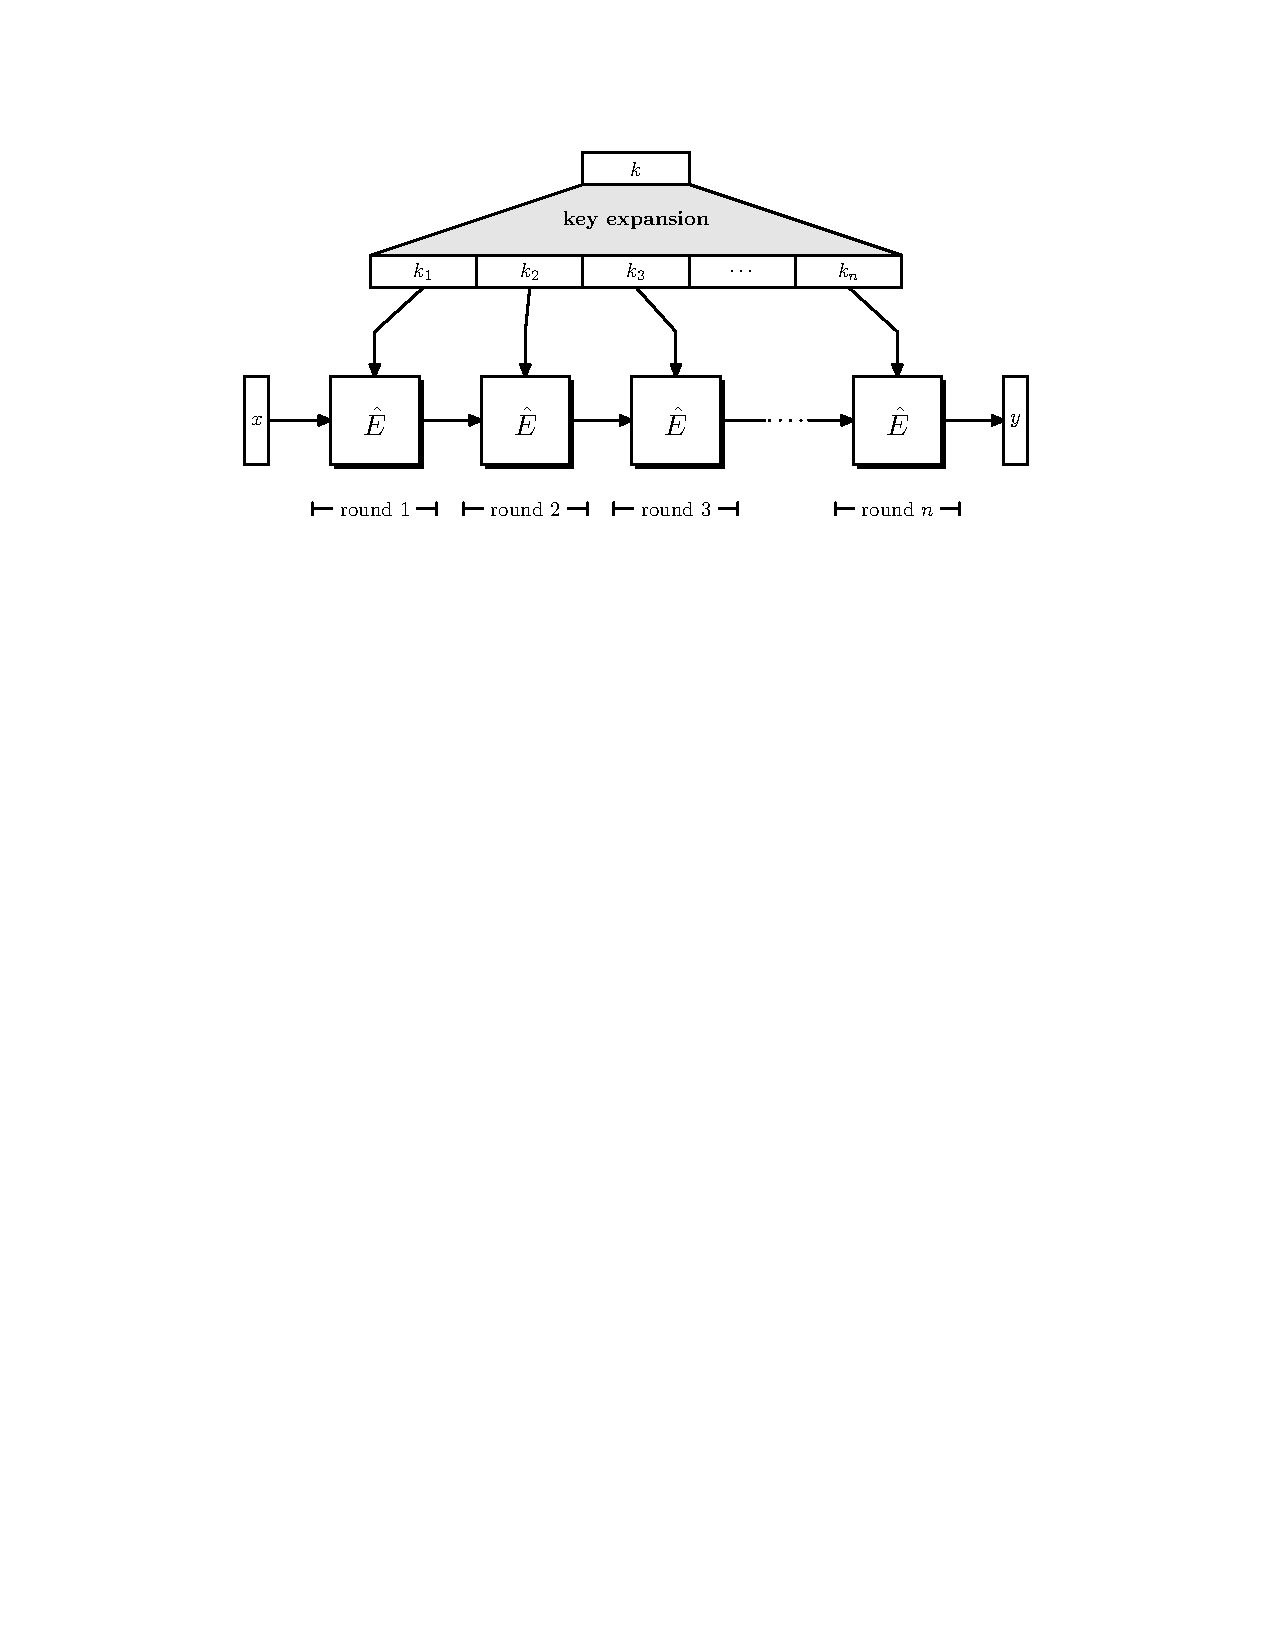
\includegraphics[scale=0.85]{crypto boneh book draft 123}\\
\captionsetup{labelsep=colon}
\caption{Figure of typical Block Cipher constructions}
\end{figure}
\paragraph{} So here we have our input message. Say, for AES, the message would be 128 bits exactly, because each block in AES is exactly 128 bits. And then the first thing that happens is we apply the first round function using the key $K_1$ to the message. And we get some new message out, as a result. Then we take this message $m_1$, we apply the next round function to it using a different key, using the key $k_2$. Then we get the next round message out. And so on and so forth until all the rounds have been applied and then the final output is actually the result of the cipher. And again this would be also in the case of AES, this was 128 bits. And the resulting cipher text would also be 128 bits. Now, different ciphers have different number of rounds, and they have different round functions.
\paragraph{} So, for example, for triple DES the number of rounds is 48. And we're going to see exactly how the round function for triple DES works. For AES, for example, the number of rounds is only ten, and again, we're going to look at how the round functions for AES work as well in just a minute. Before we do that, I just wanted to mention performance numbers. So you can see here, these are the performance numbers for the two typical block ciphers, triple DES and AES. And these are the corresponding numbers for the stream ciphers that we looked at in the previous module.And if you see that the block ciphers are considerably slower than stream ciphers. But we'll see that we can do many things with block ciphers that we couldn't do very efficiently with, constructions like RC4.
\paragraph{} Now my goal for this chapter is to show you how block ciphers work, but more importantly I want to show you how to use block ciphers correctly, for either encryption or integrity or whatever application you have in mind. So to show you how to use block ciphers correctly, it actually makes a lot of sense to abstract the concept a little bit so we have a clean, abstract concept of a block cipher to work with. And then we can argue and reason about what constructions are correct and what constructions are incorrect.
\paragraph{} And so an abstraction, it's a very elegant abstraction of a block cipher is what's called a pseudo random function, a pseudo random permutation. So let me explain what these things are. So a pseudo random function basically is defined over a key space, an input space, and an output space. And all it is, is basically a function that takes a key and an input as inputs and outputs some element in the output space.  So it takes an element in K, an element in X, and outputs an element in Y. And the only requirement essentially, is that there's an efficient way to evaluate the function. For functions we're not requiring that they be invertible, we just need them to be evaluatable, given the key and the input x.
\dfn{Pseudo random function}{A pseudo-random function (PRF) F is a deterministic algorithm that has two inputs: a key k
and an input data block x; its output $y := F(k, x)$ is called an output data block. As usual, there are associated, finite spaces: the key space K, in which k lies, the input space X, in which x lies, and the output space Y, in which y lies. We say that F is fined over $(\mathcal{K},\mathcal{X},\mathcal{Y})$. Also, an "efficient" algorithm for calculating the function must exist}
\paragraph{} Now, a related concept that more accurately captures what a block cipher is it's called a pseudo-random permutation. So a pseudo random permutation is, again, defined over a key space, and then just a set X. And what it does is it takes an element in the key space, an element of X, and outputs, basically, one element in X. Now, as usual, the function E should be easy to evaluate. So there should be an algorithm to evaluate the function E. But more importantly, once we fix the key K, it's important that this function E be one-to-one.
\dfnc{Pseudo random permutation}{A pseudo random function that has the same image set as the input space and is also invertible. The inversion function must also be "efficient"}
\paragraph{} In other words, if you think of the space X as the set here, and here's the same set X again, then basically the function E, what it does, is, it's a one-to-one function, so every element in X gets mapped to exactly one element in X. And then because it's one to one, of course it's also invertible. So given some output there's only one input that maps to that output. And the requirement is that there is an efficient inversion algorithm, call it D, that given a particular output, will output the original preimage that mapped to that output. So really, a pseudo random permutation captures very accurately and syntactically what a block cipher is, and often I'll use the terms interchangeably, either a block cipher or a pseudo random permutation. I'll use whichever term depending on the context where we're discussing things.
\paragraph{} We have two examples, as we said, of pseudorandom permutations, triple DES and AES, say for AES-128. The key space would be 128 bits and the output space would be 128 bits. For Triple DES, as we said, the block size is only 64 bits. And the key size is 168 bits, okay. So we'll use these running examples actually throughout, so whenever I say a PRP, concretely you should be thinking AES or Triple DES.
\paragraph{} Now one thing that I wanted to point out is that in fact any pseudo-random permutation, namely any block cipher, you can also think of it as a PRF. In fact a PRP is a PRF that has more structure. In particular, a PRP is a PRF where the input space and the output space are the same, so X is equal to Y, and in fact is efficiently invertible once you have the secret key k. Okay. So in some sense a PRP is a special case of a PRF, although that's not entirely accurate, and we'll see why in just a second.
\paragraph{} So, so far, we just described the, kind of, the syntactic definition of what is a pseudo random permutation and a pseudo random function. So now, let's talk about what it means for a PRF or a PRP to be secure. And this concept will essentially capture what it means for a block cipher to be secure. So this is why I wanted to show you these definitions, before we look at actual block cipher constructions, so at least it's clear in your mind what it is we're trying to construct.
\paragraph{} So here we have a PRF. And I'm going to need a little bit of notation, not too much though, so I'm going to need to define the set "Funs of X, Y". This is basically the set of all functions from the set X to the set Y, denoted here as a big circle, Funs[X, Y]. Now this set is gigantic. Its size is basically, you know, $|Y|^{|X|}$, so for example for AES, remember both X and Y would be $2^{128}$, so for AES the size of the set is enormous. It'll be $2^{128\times 2^{128}}$. So it's kind of a double exponential. So this is a gigantic number, this is more particles than there are in the Universe. But regardless, we can kind of think of this set abstractly. We never have to kind of write it down, we can just keep it in our head and not worry about computing on it.
\paragraph{} So this is a particular gigantic set of the set of all functions from X to Y. Now we're going to look at a much smaller set of functions, namely I'll call this set S sub F, and that's going to denote the set of all functions from X to Y that are specified by the PRF as soon as we fix the particular key k. We fixed the key k, we let the second argument float, and that basically defines a function from X to Y. Then we're going to look at the set of all such functions for all possible keys in the key space. So, if you think about it again, for AES, if we're using 128-bit keys, the size of this, I'll say S-AES, is basically going to be $2^{128}$, so much, much smaller than the set of all possible functions from X to Y. So we literally, we pick some arbitrary function in this gigantic set of all functions from X to Y. And we say that the PRF is secure, if, in fact, a random function from X to Y is indistinguishable from a pseudo-random function from X to Y.
\paragraph{} Namely, when we pick a random function from the set SF. So, more precisely again, the uniform distribution on the set of pseudo random functions is indistinguishable from the uniform distribution on the set of all functions. Let me be just a little bit more precise, just to give you a little bit more intuition about what I mean by that and then we'll move on to actual constructions.
\paragraph{} 
\begin{note}
Let me a bit more precise about what it means for a PRF to be secure. And so what we'll do is basically the following. So we have our adversary, who's trying to distinguish truly random function from a pseudo random function. So what we'll do is let them interact with one of the two. So here in the top cloud, we're choosing a truly random function. In the bottom cloud, we're just choosing a random key for a pseudo random function. And now what this adversary's going to do is he's going to submit points in X. So he's going to submit a bunch of Xs. In fact, he's going to do this again and again and again. So he's going to submit $X_1$, $X_2$ ,  $X_3$, $X_4$, and then for each one of, of those queries, we're going to give him either the value of the truly random function at the point X, or the value of the pseudo random function at the point X.  So the adversary doesn't know which ones he's getting. By the way, for all queries, he's always getting either the truly random function, or the pseudo random function. In other words, he's either interacting with a truly random function for all his queries, or he's interacting with a pseudo random function for all his queries. And we say that the PRF is secure if this poor adversary can't tell the difference. He cannot tell whether he's interacting with a truly random function or interacting with a pseudo random function.
\end{note}
\paragraph{} We're going to come back actually later on and define PRFs more precisely but for now, I wanted to give you the intuition for what it means for PRFs to be secure so you'll understand what it is that we're trying to construct when we construct these pseudo random functions. And I should say that the definition for a pseudo random permutation is pretty much the same, except instead of choosing a random function, we're going to choose a random permutation on the set X. In other words, a random one-to-one function on the set X. The adversary can either query this random function on the set X, or he can query a pseudo random permutation, and the PRP is secure if the adversary cannot tell the difference. So again the goal is to make these functions and permutations look like truly random functions or permutations. 
\qs{}{Let's look at a simple question. So suppose we have a secure PRF. So we know this PRF F. Happens to be defined in the set X. And it so happens, you know, it outputs 128 bits every time. It so happens that this PRF cannot be distinguished from a truly random function from X to $\{0,1\}^{128}$. Now we're going to build a new PRF. Let's call this PRF G. And the PRF G is going to be defined as follows. We say, if X is equal to zero, always output zero. Otherwise, if X is not equal to zero, just output the value of F. So, my question to you is, do you think this G is a secure PRF?}
\sol Well, so, the answer, of course, is that its very easy to distinguish the function G from a random function. All the adversary has to do is just query the function at X=0. For a random function, the probability that the result is going to be zero is one over $2^{128}$. Whereas for the pseudo-random function, he's always going to get zero. Because at zero, the function is always defined to be zero, no matter what the key. And so all he would do is he would say, hey, I'm interacting with a pseudo-random function if he gets zero at X=0, and he'll say I'm interacting with a random function if he gets nonzero at X=0. So it's very easy to distinguish this G from random. 
\paragraph{} What this example shows is that even if you have a secure PRF, it's enough that on just one known input the output is not random, the output is fixed, and already the PRF is broken, even though you realize that everywhere else the PRF is perfectly indistinguishable from random. So let's just show you the power of PRFs. Let's look at a very easy application. I want to show you that in fact pseudo random functions directly give us a pseudo random generator. 
\paragraph{} Let's assume we have a pseudo random function. So this one happens to go from N bits to N bits. And then, let's define the following generator. Its seed space is going to be the key space for the PRF, and its output space is going to be, basically, t blocks of N bits each. therefore you can see the output is a total of N times t bits for some parameter t that we can choose. And it turns out, basically, you can do this very simple construction, this is sometimes called counter mode, where essentially, you take the PRF and you evaluate it at zero, you evaluate it at one, you evaluate it at two, at three, at four, up to t, and you concatenate all these values. 
\dfn{Counter mode PRF}{Suppose we have a PRF $F:\mathcal{K}\times \{0,1\}^N\rightarrow \{0,1\}^N$. Then a PRG $G:\mathcal{K}\rightarrow \{0,1\}^{Nt}$ construction is as follows:
\[
G(k)=F(k,0)||F(k,1)||\ldots F(k,t-1)
\]
}
\thm{}{If the PRF defined above is secure, the resulting PRG is also secure}
\paragraph{} That's the generator. So we basically took the key for the PRF and we expanded it into n times t bits. Okay. A key property of this generator is that it's parallelizable. What I mean by that is if you have two processors or two cores that you can compute on, then you can have one core compute the even entries of the output, and you can have another core compute the odd entries of the output. So basically, if you have two cores, you can make this generator run twice as fast as it would if you only have a single core. So the nice thing about this is, of course, we know that pseudo-random generators give us stream ciphers, and so this is an example of a parallelizable stream cipher. And I just wanted to point out that many of the stream ciphers that we looked at before, for example, RC4, those were inherently sequential. So even if you had two processors, you couldn't make the stream cipher work any faster than if you just had a single processor.
\paragraph{} Now the main question is why is this generator secure? And so here I'm only going to give you a little bit of intuition and we're going to come back and argue this more precisely later on. But I'll just say that security basically falls directly from the PRF property. And the way we reason about security, is we say, well this PRF by definition is indistinguishable from a truly random function on 128 bits. So in other words, if I take this generator and instead I define a generator using a truly random function, in other words, I'll write the output of the generator as f(0) concatenated f(1), and so on and so forth, using a truly random function, then the output of the generator using the truly random function would be indistinguishable from the output of the generator using a pseudorandom function. That is the essence of the security property of a PRF.
\paragraph{} But with a truly random function, you notice that the output is just truly random. Because for a truly random function, f(0) is a random value. f(1) is an independent random value. f(2) is an independent random value, and so on and so forth. So the entire output is a truly random output. And so with a truly random function, a generator produces truly random outputs, and is therefore a perfectly secure generator. And so you see how the PRF security property lets us argue security. Basically, we argue that when we replace the PRF with a truly random function, the construction is necessarily secure, and that says that the construction with a pseudorandom function is also secure.  And we're going to see a couple more examples like this later on. So now you understand what a block cipher is, and you have intuition for what security properties it's trying to achieve. And in the next part, we're going to look at constructions for block ciphers.

\section{Block Ciphers 2: The Data Encryption Standard}
\subsection{The Data Encryption Standard}
So now that we understand what block ciphers are, let's look at a classic example called the Data Encryption Standard. So, just a quick reminder. Block ciphers basically map N bits of input to N bits of output. And we talked about two canonical examples, Triple DES and AES. In this part, we're going to talk about DES, and we'll talk about Triple DES, actually, in the next part. And then I also mentioned before that block ciphers are often built by iteration. In particular, we're going to look at block ciphers that are built by a form of iteration where a key K is first expanded into a bunch of round keys. And then a round function is applied to the input message, again and again. And essentially, after all these round functions are applied, we obtain the resulting cipher text. 
\paragraph{} And again, what we're going to look at, how DES, the data encryption standard, uses this format. I just want to be clear that, in fact, to specify a block cipher of this type, one needs to specify the key expansion mechanism, and one needs to specify the round function. In the section here, I'm going to focus on the round function, and I'm not going to talk much about key expansion. But I just wanted to mention that, in fact, key expansion is also a big part of describing how block cipher works.
\begin{note}
\paragraph{} Let's talk about the history of DES. Essentially, in the early 1970s, IBM realized that their customers are demanding some form of encryption. And so they formed a crypto group, and the head of that group, was Horst Feistel, who, in the early 70s, designed a cipher called Lucifer. It's interesting. In fact Lucifer had a number of variations but one of the later variations in fact had a key length that was 128 bits and a block length that's also 128 bits.
\paragraph{} In 1973 the governor realized that it's buying many commercial off-the-shelf computers and so it wanted its suppliers to actually have a good grip to algorithm that they could use in products sold to the government. So in 1973 the National Bureau of Standards as it was called at the time put out a request for proposals for a block cipher that is going to become a federal standard. And in fact IBM submitted a variant of Lucifer. That variant actually went through some modification during the standardization process and then finally in 1976, the national bureau standard adopted DES as a federal standard. And, in fact, for DES it's interesting that the key length was far reduced from Lucifer. It's only 56 bits. And the block length was also reduced to 64 bits. And in fact, these decisions, especially the decision to reduce the key length, is going to be a key length yield of DES and was a source of many complaints over its life. 
\paragraph{} In particular, already back in 1997, DES was broken by exhaustive search meaning that a machine was able to search through all $2^{56}$ possible keys to recover a particular challenge key. And in fact we're going to talk about exhaustive search quite a bit. It's quite an interesting question, and there are various ways to defend against exhaustive search. And basically this 1997 experiment spelled the doom of DES. It meant that DES is itself, is no longer secure. And as a result, the National Institute of Standards, as it became known, issued a request for proposals. For our next generation's block cipher standard and in 2000 it standardized on a cipher called Rijndael. Which became the advanced encryption standard, AES. And we'll talk about AES later on.
\end{note}
\paragraph{}
 But in this part, I want to describe how DES works. Now, DES is a cipher, it's an amazingly successful cipher. It's been used in the banking industry. In fact, there's a classic network called the \underline{Electronic Clearinghouse}, which banks use to clear checks with one another. And DES is used for integrity in those transactions. It's also used in commerce. In fact, it was very popular up until recently, as the main encryption mechanism for the web. Of course, now, that's been replaced with AES and other ciphers. Overall, it's a very successful cipher in terms of deployment. DES also has a very rich history of attacks, which we'll talk about in the next part.
 \paragraph{} Now, let's talking about the construction of DES. So, the core idea behind DES is what's called a Feistel network, due to Horst Feistel. And basically, it's a very clever idea for building the block cipher out of arbitrary functions, $F_1$ to $F_d$. Imagine we have these functions $F_1$ to $F_d$ that happens to match n bits to n bits. Now these are arbitrary functions, they don't have to be invertible or anything. What we want to do is build an invertible function out of those d functions and the way we'll do it is by building a new function we'll call capital \textbf{f} that maps 2n bits to 2n bits. And the construction is described right here. So here we have our inputs. You notice, there are two blocks of n bits. In other words, the input is actually 2n bits. The R and L stand for right and left.
 \begin{figure}[H]
\centering
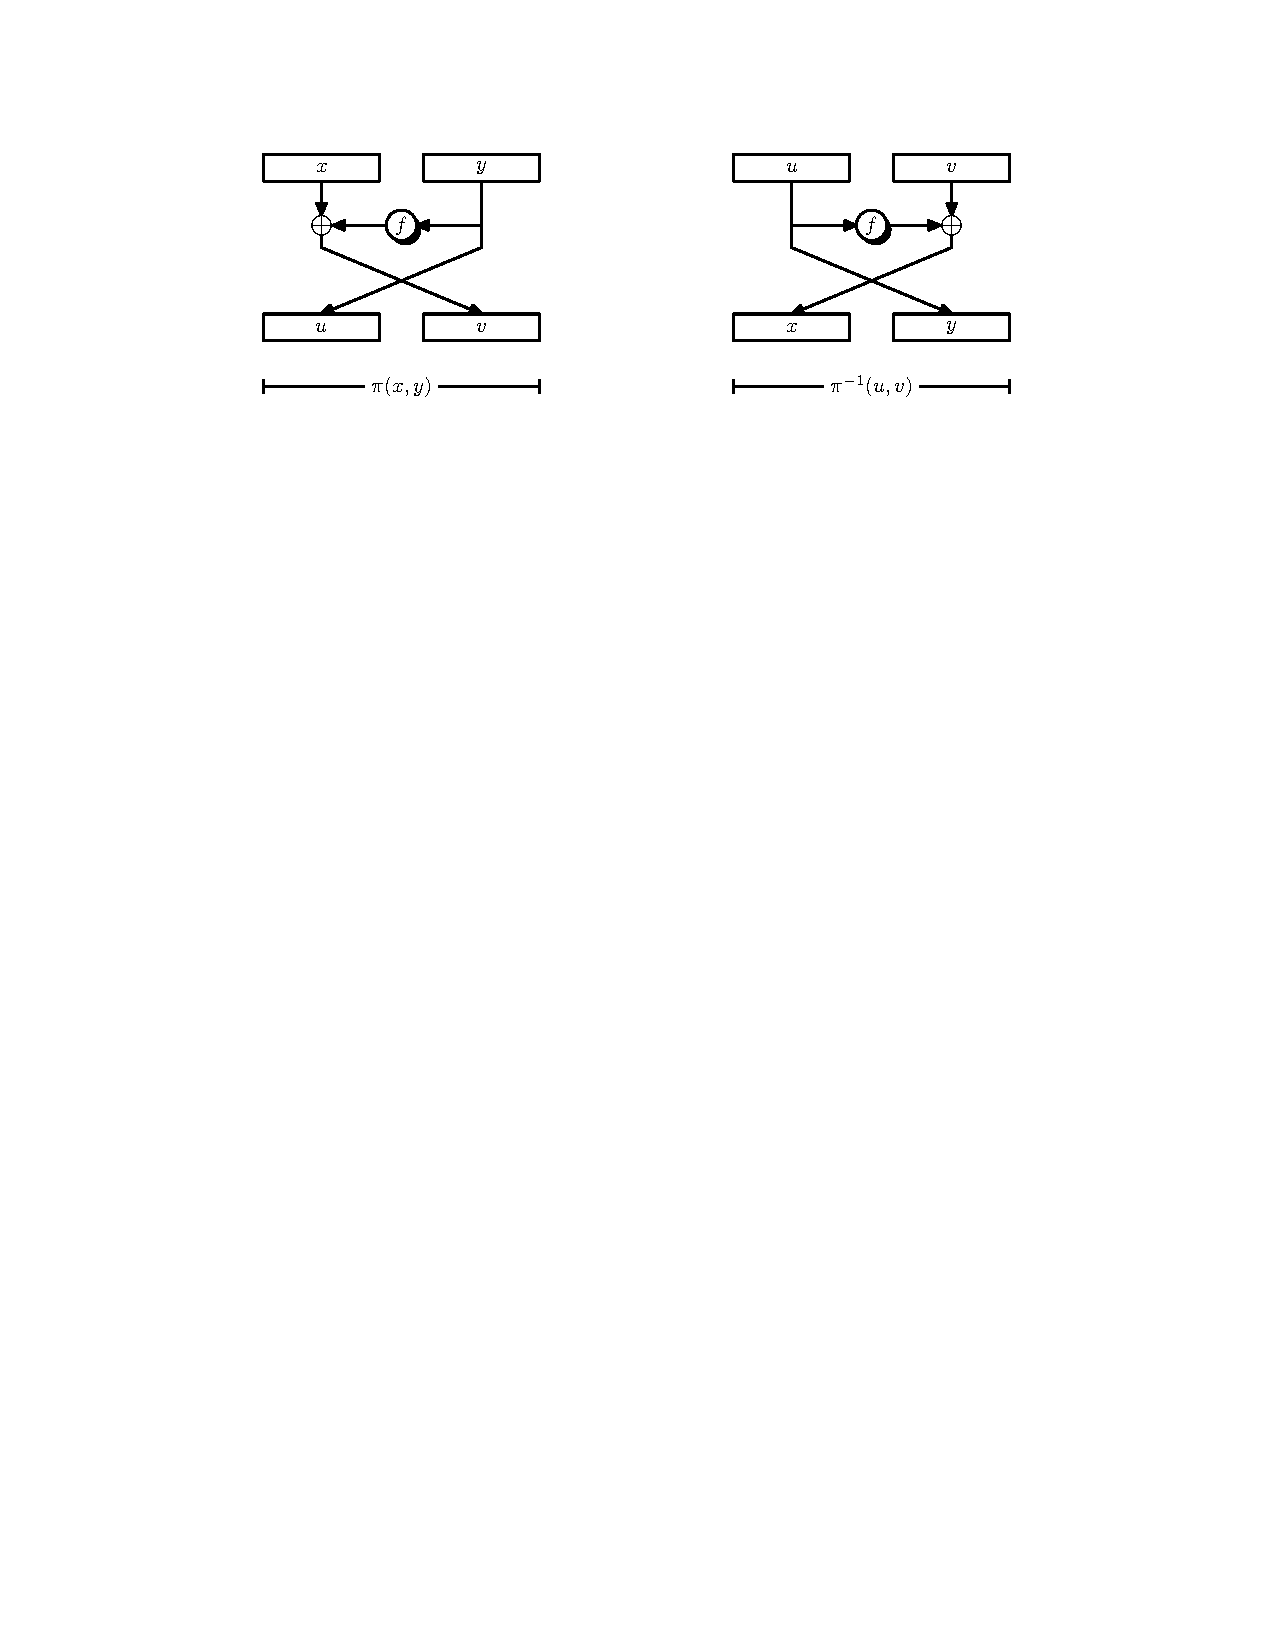
\includegraphics[scale=0.85]{crypto boneh book draft 126}\\
\captionsetup{labelsep=colon}
\caption{Feistel Network component and its inverse}
\end{figure}

\begin{figure}[H]
\centering
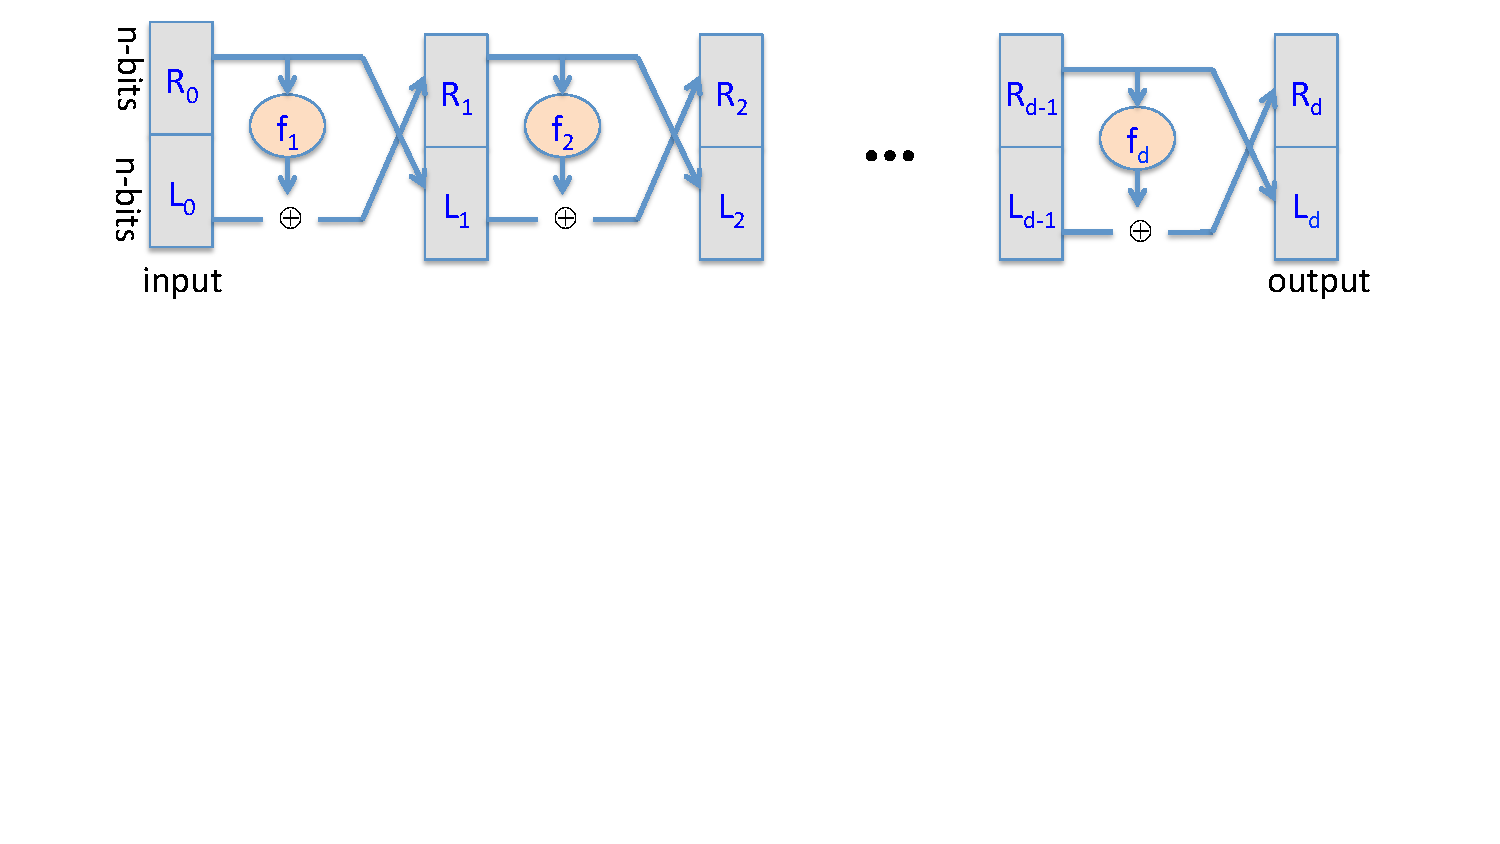
\includegraphics[scale=0.55]{03-block-v2-annotated 18}\\
\captionsetup{labelsep=colon}
\caption{Multiple rounds of Feistel Networks}
\end{figure}
  Typically, people describe a Feistel network from top to bottom. In which case, these n bits really would be right and left. But here it is more convenient for me to describe it horizontally. So if we follow the R inputs. You realize it basically gets copied into the L output, without any change at all.  However, the L inputs, is changed somewhat. What happens is, basically, the R inputs is fit into the function $F_1$ and the result is then XORed with $L_0$ and that becomes the new R1 input. Okay, so this is called one round of a Feistel network, and is done using the function $F_1$. Now we do this again with another round of the Feistel network with the function $F_2$, and we do it again and again , until we get to the last round, and we do it again with the function $F_d$. And finally, the output is $R_d, L_d$. Okay. So, if you like, we can write this in symbols. That basically, $L_i$ is simply equal to $R_{i-1}$. And $R_i$, let's see, that's the more complicated one. Well, let's just follow the lines here. $R_i$ is just equal to $F_i$ applied to, $R_{i-1}\oplus L_i$. This is basically, i goes from, 1 to d. So this is the equation that defines a Feistel network, mapping a 2n bit input to 2n bit outputs.
  \clm{Feistel Network is invertible}{}{ And the amazing claim is that, in fact, it doesn't matter which functions you give me. For any functions, $F_1$ to $F_d$ that you give me, the resulting Feistel network function is, in fact, invertible. And the way we're going to prove that is basically we're going to construct an inverse, because not only is it invertible, it's efficiently invertible.}
  \proof So let's see. So let's look at one round of a Feistel network, so here, this is the inputs, $R_i,L_i$, and this is the output $R_{i+1},L_{i+1}$. And now what I'm going to ask you is to invert this. Suppose now the input that we're given is $R_{i+1},L_{i+1}$ and we want to compute $R_i,L_i$. Well, let's look at $R_i$. Basically, $R_i$ is just equal to $L_{i+1}$. So $L_{i+1}$ just becomes $R_i$. But now, let me ask you, to write the expression for $L_i$ in terms of $R_{i+1},L_{i+1}$. I hope everybody sees that, basically, $L_{i+1}$ is fed into the function $F_{i+1}$. The result is XORed with $R_{i+1}$, and that gives the $L_i$ input.
  \paragraph{} So you notice that the inverse of a Feistel round looks pretty much the same as the Feistel round in the forward direction. It's literally, you know, just for a technical reason, it's kind of the mirror image of one another. But it's basically, the same construct. And when we put these inverted rounds back together. We essentially get the inverse of the entire Feistel network.
\begin{figure}[H]
\centering
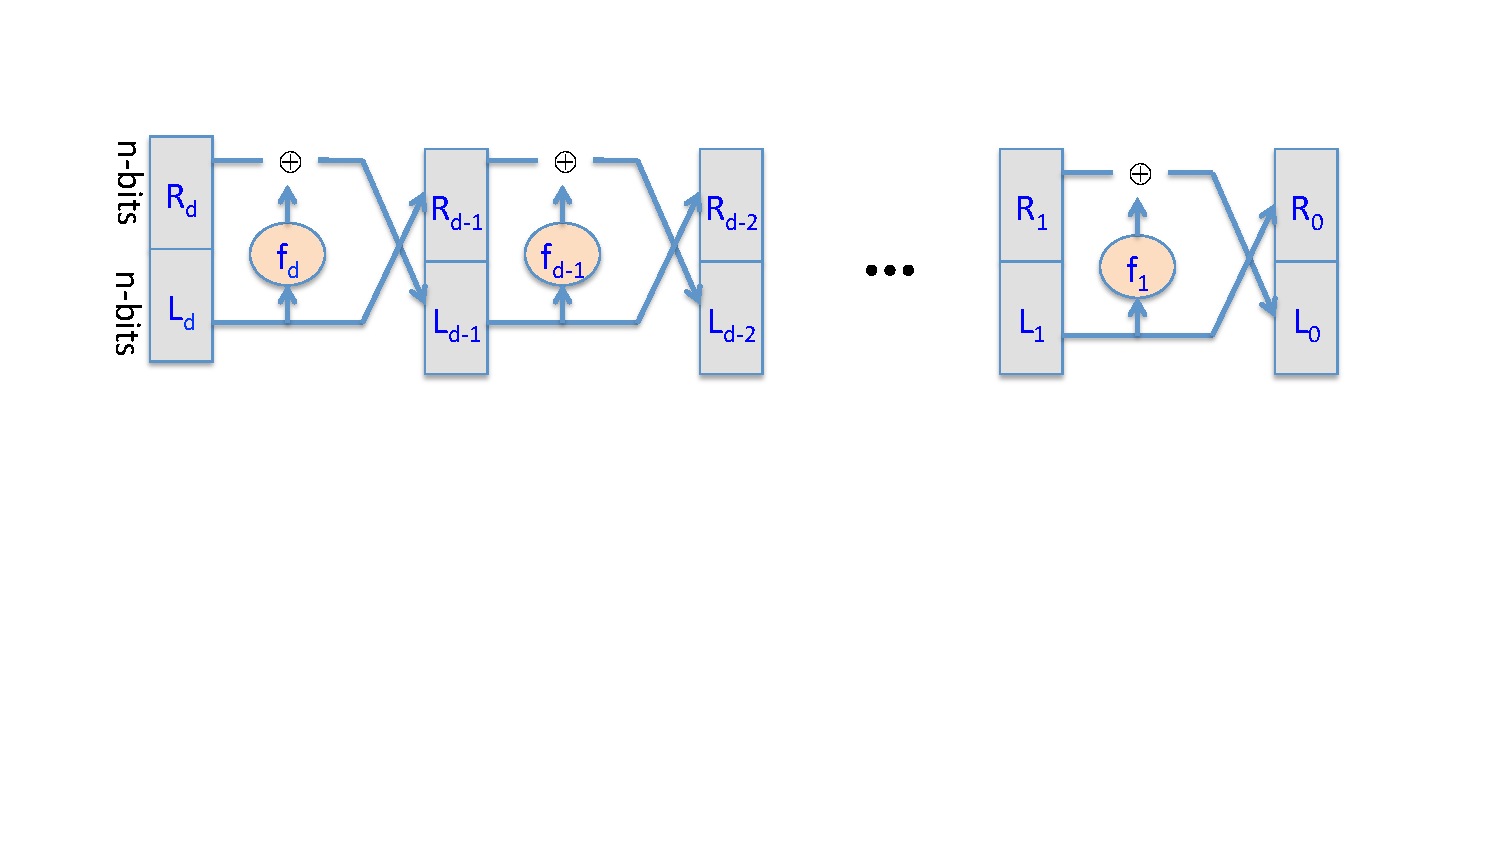
\includegraphics[scale=0.55]{03-block-v2-annotated 20}\\
\captionsetup{labelsep=colon}
\caption{Inverse Feistel Network}
\end{figure}  
\paragraph{}
   So you notice we start off with the round number \textbf{d} with the inverse of round number \textbf{d}, then we do the inverse of round number \textbf{d-1} and so on and so forth until we get to the inverse of the first round. And we get our final outputs which is $R_,L_0$, like this is the inputs and we manage to invert basically $R_d,L_d$ and get $R_0,L_0$ and the interesting thing is that basically these inversion circuits look pretty much the same as the encryption circuits and the only difference is that the functions are applied in reverse order. Right we started with $F_d$ and ended with $F_1$. Whereas when we were encrypting, we started with $F_1$ and ended with $F_d$. So, for hardware designers, this is very attractive, because, basically, if you want to save hardware, you realize that your encryption hardware is identical to your decryption hardware. So you only have to implement one algorithm, and you get both algorithms the same way. The only difference is that the functions are applied in reverse order.
   \paragraph{}  So this Feistel mechanism is a general method for building invertible functions from arbitrary functions $F_1$ to $F_d$ and in fact, it's used in many different block ciphers. Although, interestingly, it's not actually used in AES. So, there are many other block ciphers that use a Feistel network. Or, of course, they differ from DES in the functions $F_1$ to $F_d$. But AES actually uses a completely different type of structure that's actually not a Feistel network. We'll see how AES works in a couple of segments.

   \paragraph{} So now that we know what Feistel networks are, let me mention an important theorem about the theory of Feistel networks that shows why they're a good idea. This theorem is due to Luby and Rackoff back in 1985, and it says the following.
   \thm{Security of Three-round Feistel Network}{If f is a secure PRF for n bits, the three-round Feistel Network with identical PRFs in differnet blocks (but with a different key for each block) is a secure PRP for 2n bits ($F: \mathcal{K}^3\times \{0,1\}^{2n}\rightarrow \{0,1\}^{2n})$.}
   \paragraph{} Suppose I have a function that is a secure pseudorandom function.So it's indistinguishable from random and happens to act on n bits. So it maps n bits to n bits and uses a key K. Then, it turns out, that if you use this function in three rounds of a Feistel network. What you end up with is a secure pseudo random permutation. In other words, what you end up with is an invertible function that is indistinguishable from a truly random invertible function. And I hope you remember that the true definition of a secure block cipher is that it needs to be a secure pseudo random permutation. So what this theorem says, is that if you start with a secure pseudo random function, you end up with a secure block cipher. 
\paragraph{} Let me explain in a little bit more detail what's actually going on here. So, essentially, the PRF is used in every round of the Feistel network. So, in other words, here, what's actually computed is the PRF using one secret key, $K_0$. Here, what's computed is the PRF using a different secret key, of course applied to R1. And here we have yet another secret key, $K_1$ applied, $K_2$ applied to $R_2$. And you notice, this is why, basically this Feistel construction, uses keys in $\mathcal{K}^3$. In other words, it uses three independent keys. So it's very important that the keys are actually independent. So really, we need three, independent keys. And then we end up with a secure pseudorandom permutation.
\paragraph{} So that's the theory behind Feistel networks. And now that we understand that, we can actually look at the specifics of DES. DES is basically a sixteen round Feistel network, okay. So there are functions $F_1$ to $F_16$ that map 32 bits to 32 bits, and as a result, the DES itself acts on 64 bit blocks. Now the sixteen round functions in DES are actually all derived from a single function \textbf{f}. Just used with different keys. So in fact, these are the different round keys. So $k_i$ is, a round key. And it's basically derived from the key K, derived from the 56 bit DES key K.
\begin{figure}[H]
\centering
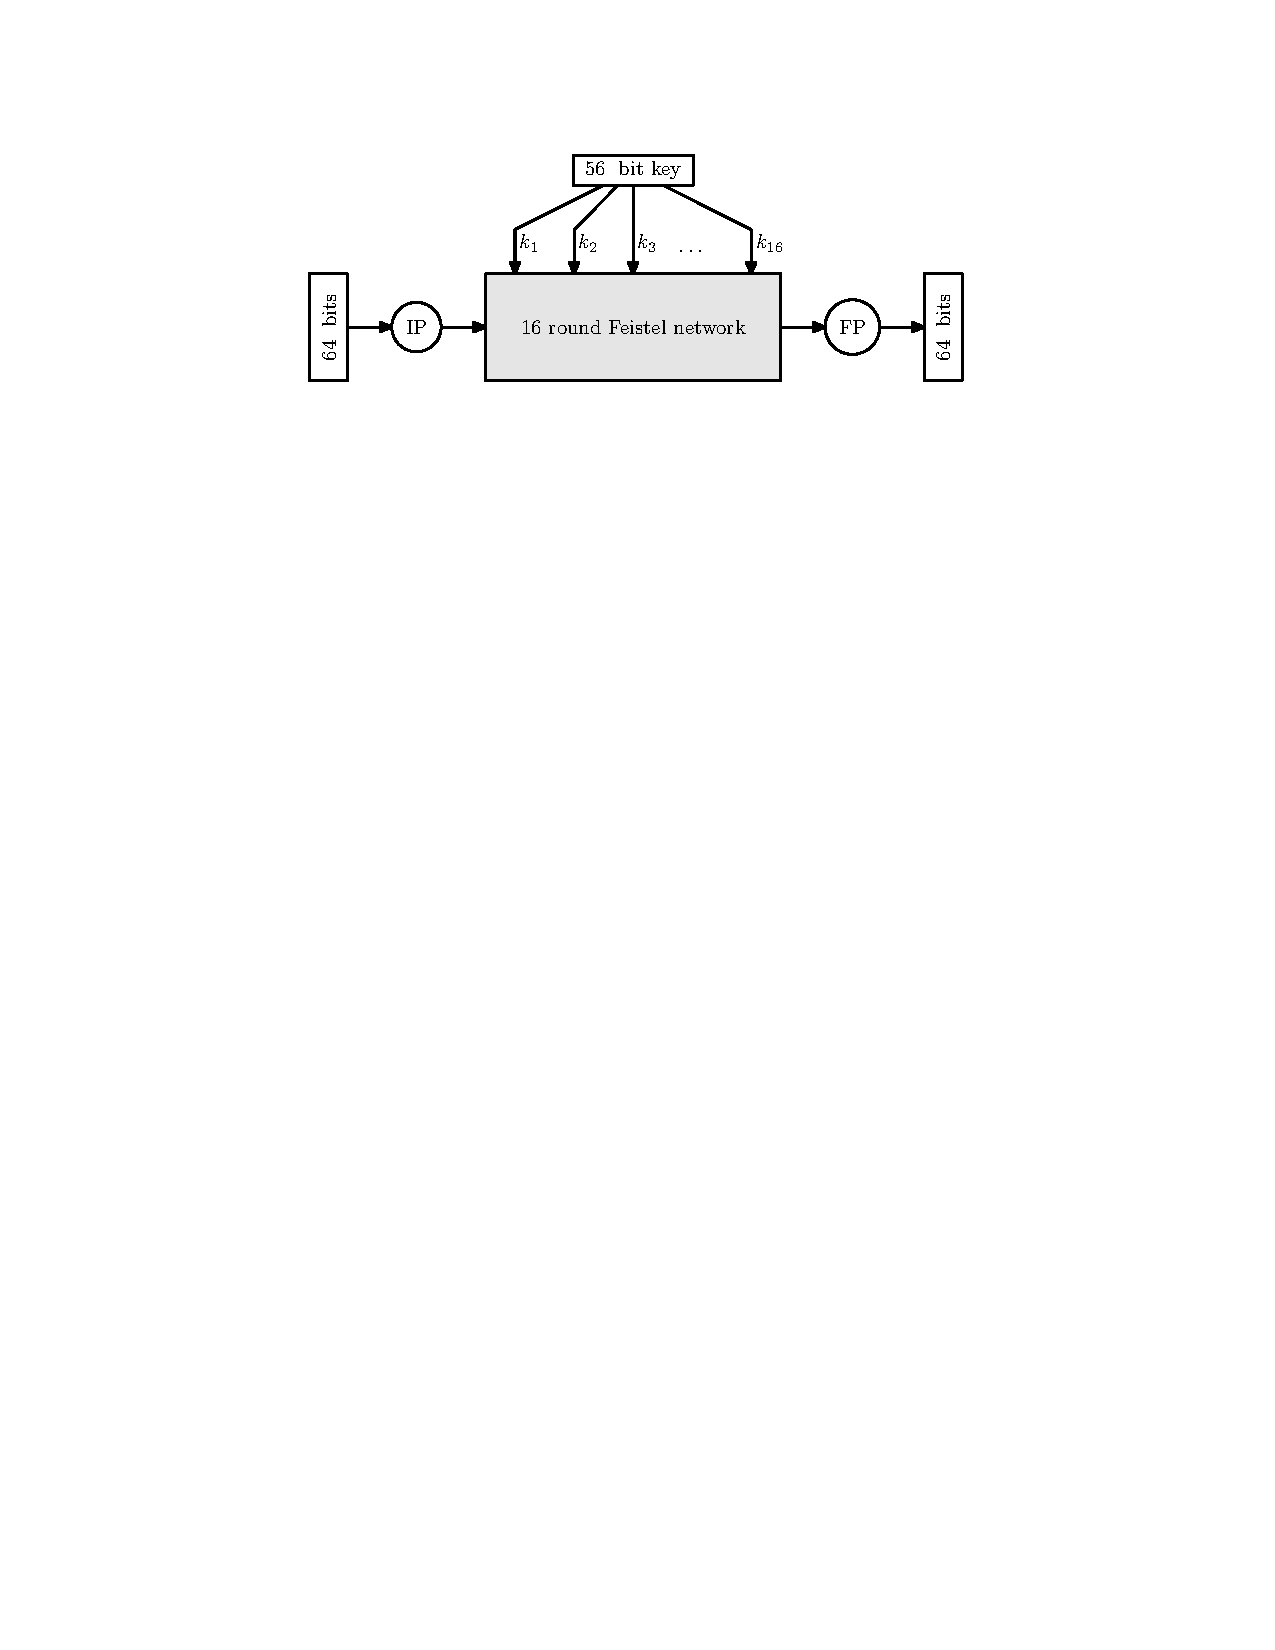
\includegraphics[scale=0.85]{crypto boneh book draft 129}\\
\captionsetup{labelsep=colon}
\caption{DES full circuit}
\end{figure}
\paragraph{}
 I'll describe what this function \textbf{f} is in just a minute. But basically that, you see that by using sixteen different round keys, we get sixteen different round functions. And that gives us the Feistel network. So just on a high level how the DES works basically you have a 64 bit input. The first thing it does is, this initial permutation that just permutes the 64 bits around. Namely it maps bit number one to bit number six. Bit number two to bit number seventeen, and so on. This is not for security reasons, this is just specified in the standard. Then we go into the sixteen round Feistel network. That actually, you now know how it works. Basically uses the function $F_1$ to $F_16$, as specified before. And then, basically we have another permutation, it's called the final permutation. That's just the inverse of the initial permutation. Again, it just permutes bits around, this is not necessary for security reasons. And then we finally get, the final outputs.
 \paragraph{}  Now, as we said, there's a key expansion step, which I'm not going to describe. But basically, this 56-bit DES key is expanded into these rounds keys. Where each round key, is 48 bits. Okay, so we have sixteen 48 bit round keys, and they're basically used in the sixteen rounds of DES. And then when you want to invert the cipher, all you do is you use these, round keys, these 16 round keys, in reverse order.  So now that we understand the DES structure, the only thing that's left to do is specify the function, \textbf{F}. So let me explain how this function works. So basically, it takes, as inputs, its, 32 bit value, let's call it X. But in reality, you remember, this is $R_0$, $R_1$, $R_2$, $R_3$, so on and so forth. These are 32 bit values. And then it takes, also, a 48 bit round key. So here we have our key $k_i$, which happens to be 48 bits.
\begin{figure}[H]
\centering
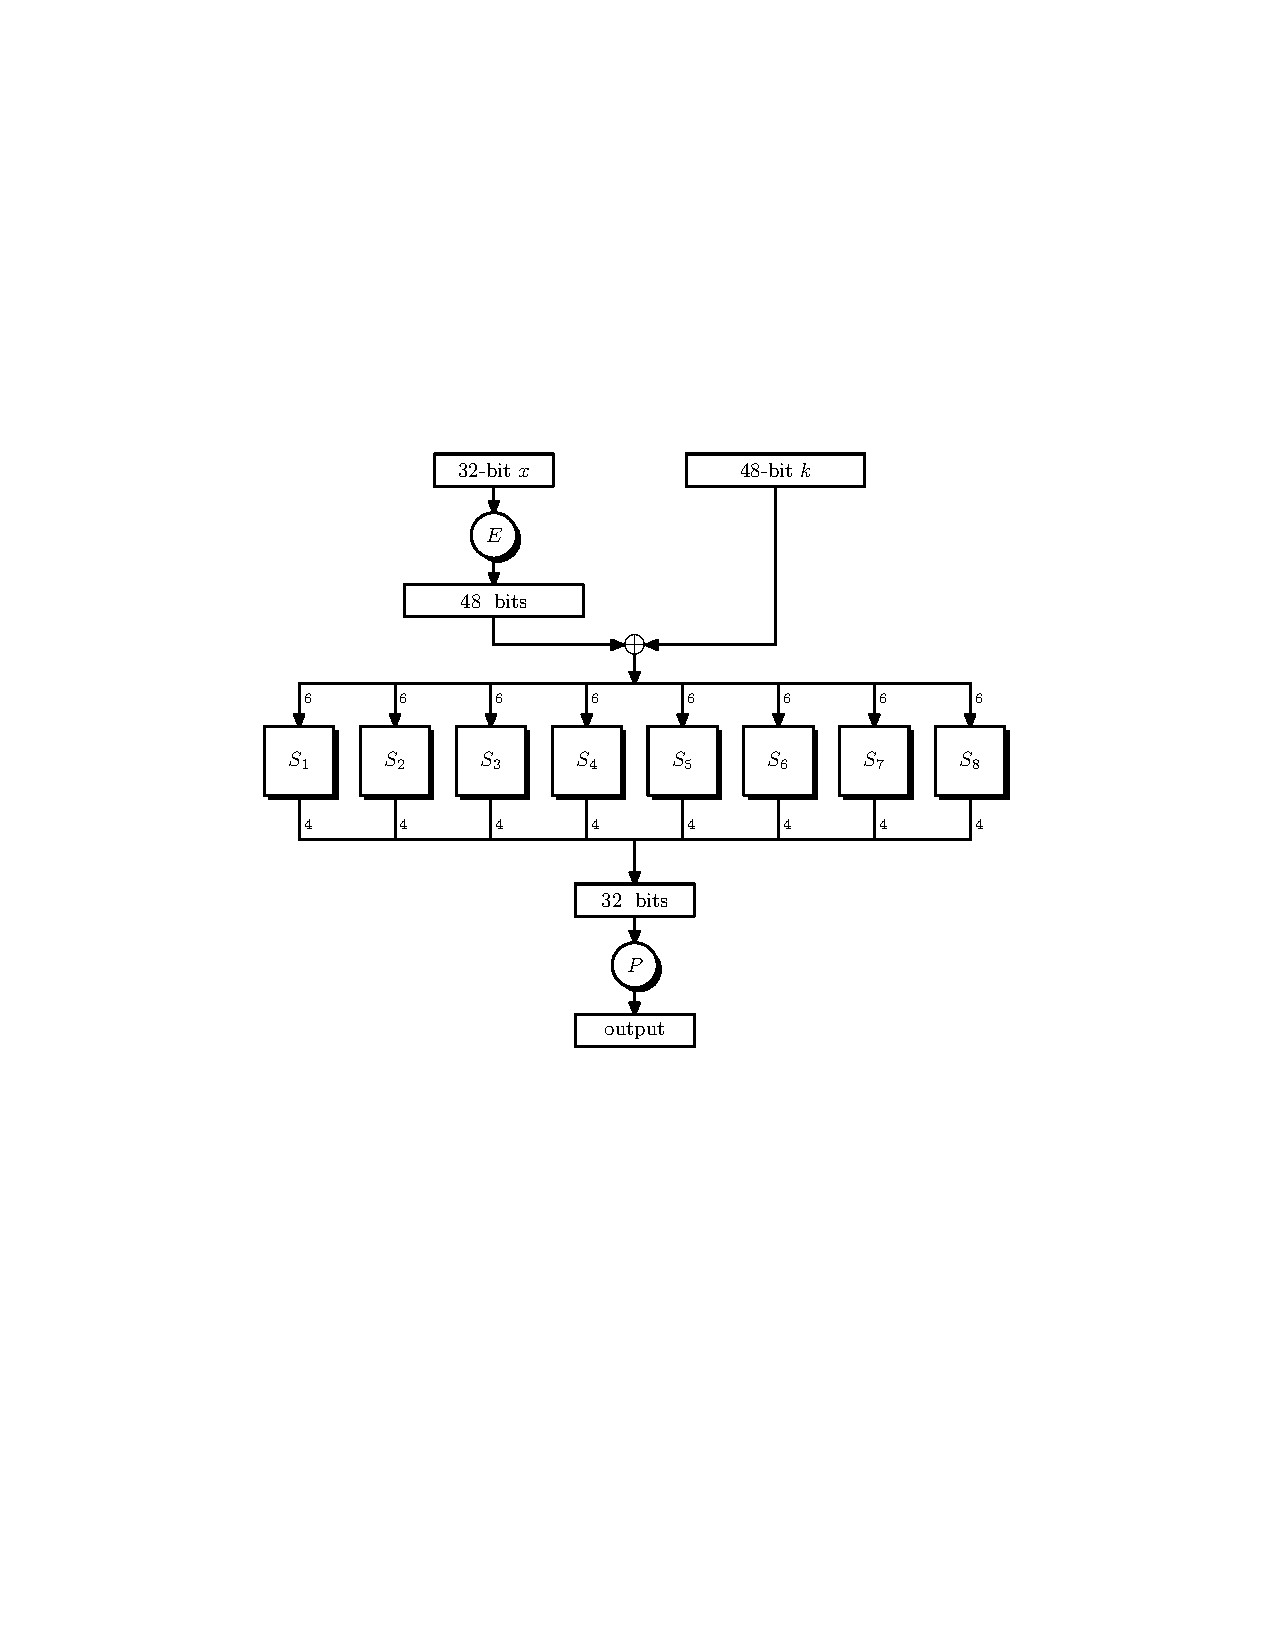
\includegraphics[scale=0.55]{crypto boneh book draft 127}\\
\captionsetup{labelsep=colon}
\caption{The PRF in DES}
\end{figure} 
 \paragraph{} The first thing it does, is it goes through an expansion box. And this expansion box basically take thirty two bits, and maps them into 48 bits. Now, all the expansion box does is just replicates some bits, and move other bits around. So, for example, bit 1 of X is replicated into positions 2 and 48 in the output. Bit 2 of X is positioned in as bit 3 of the output. And so on and so forth, just by replicating some of the bits of X, we expand the input into 48 bits. The next thing we do is we compute an XOR with the round key. Sometimes people say that cryptographers only compute XORs. This is an example of that, where, well, we just do XORs in this function. And then comes the magic of DES, where, actually, these 48 bits are broken into eight groups of six bits. Six, seven, eight. And so let me draw, and then what happens is.
 \paragraph{} Each one of these, each one of these wires is, 6 bits. And then they, they go into what, what are called S boxes. The S boxes are kind of the smarts of, DES. And then, the S box is basically a map, six bits to four bits. So, the outputs of the S boxes are these four bits. They're collected. This gives up 32 bits. Eight groups of four bits, gives us 32 bits and then finally this is fed into yet another permutation which just maps the bits around. So, for example bit number one will go to bit number nine, bit number two will go to bit number fifteen and so on. So it just permutes the 32 bits around and that's the final 32 bit output of this \textbf{F} function. So by using different round keys, essentially, we get different round functions, and that's how we form the sixteen round functions of DES.
 \paragraph{} Now, the only thing that, left to specify are these S boxes. So the S boxes, literally, are just functions from six bits to four bits. They are just implemented as a look up table. So describing a function from 6 bits to 4 bits basically amounts to writing the output of the function on all $2^{6}$  possible inputs.
\begin{figure}[H]
\centering
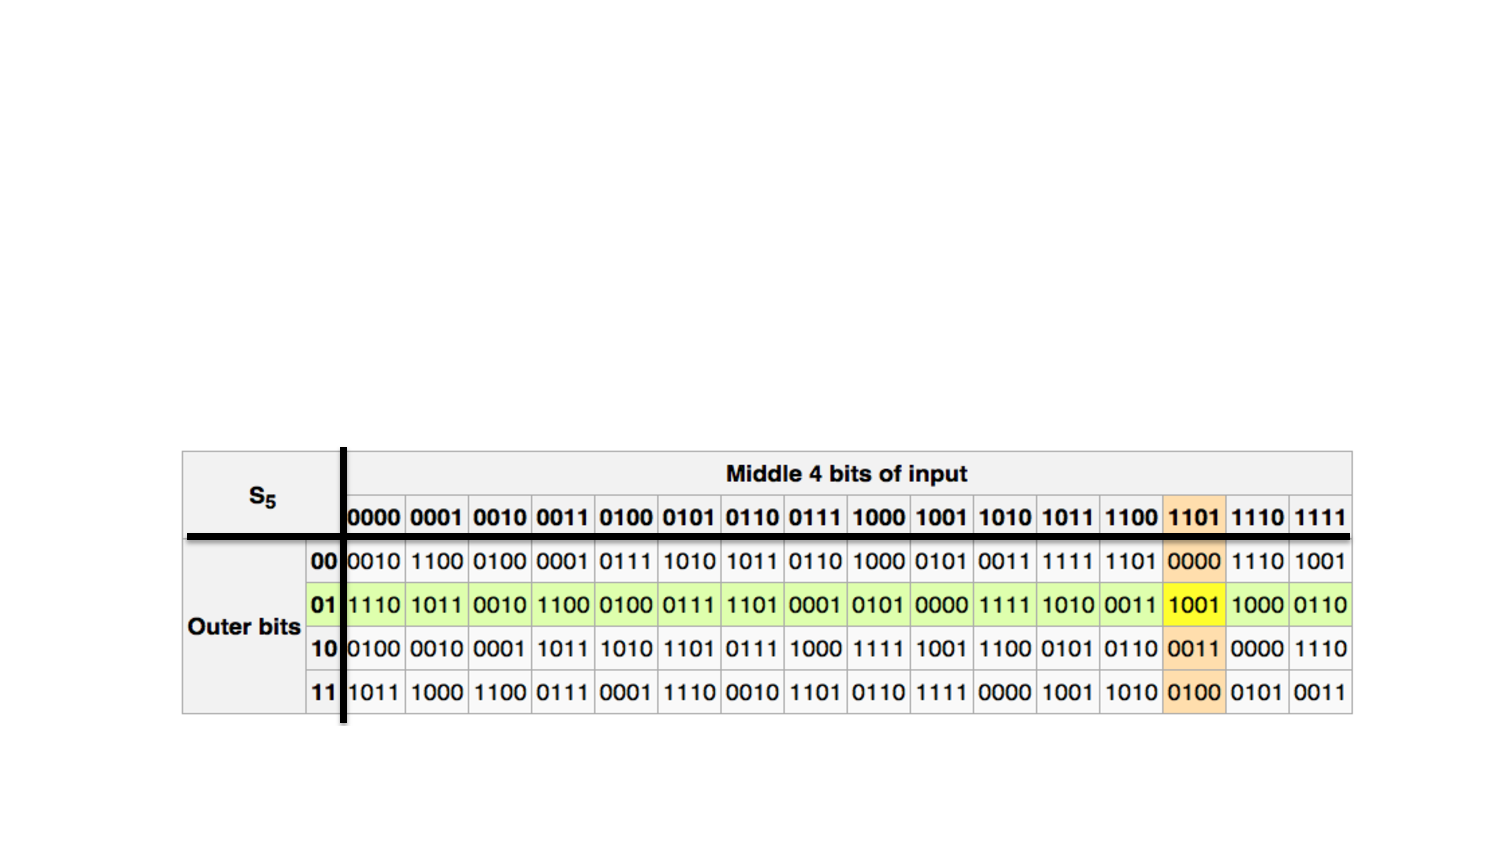
\includegraphics[scale=0.55]{03-block-v2-annotated 24}\\
\captionsetup{labelsep=colon}
\caption{S-box figure}
\end{figure} 
  So we just have a table that literally contains 64 values. Where each value is four bits. So here is an example, this happens to be the fifth S box, and you see that this is a table that contains 64 values right? It's four by 16. So, 64 values. For example, if you want to look at, the output, that corresponds to 011011. Okay, then you look at these two bits. This is 01, and these four bits are 1101, and you see that the output is 1001. The four bits output 1001.  So the S boxes are just implemented as these tables. Now the question is, how are these S boxes chosen. How are these tables actually chosen by the designers of this.
  \paragraph{} So to give you some intuitions for that, lets start with a very bad choice for S boxes. So imagine the S boxes were linear. I mean that imagine that these six bit inputs literally were just XORed with one another in different ways to produce the four bit outputs. Another way of writing that is that we can write the S box as a matrix vector product. So here you have the matrix $A_i$. And the vector, the six bit vector X. And you can see that, if we write this matrix vector product, basically, we take the inner product of this vector with the input vector. $S_i(x)=A_i.x$ (mod 2)
  \paragraph{} Remember, these are all bits. So the six bits vector inner product. Another six bit vector, and we do that modulo two, you realize, basically, what we're computing is $X_2$ XOR $X_3$. Because only position two and position three have 1's in it. And similarly the next, inner product will produce $X_1$ XOR $X_4$ XOR $X_5$ and so on and so forth. Okay. So you can literally see that if the S boxes are implemented this way. Then, all they do, is just apply the matrix A to the input vector X. Which is why we say, that in this case the S boxes are completely linear.
  \paragraph{} Now, I claimed that in fact that if the S boxes were linear, then DES would be totally insecure. The reason is, if the S boxes are linear, then all that DES does is just compute XOR of various things and permute and shuffle bits around. So it's just XORs and bit permutations, which means that as a result, all of DES is just a linear function. In other words, there will be a matrix B that has width 832. Basically what I will do is I will write the 64 bit message plus the sixteen round keys as one long vector. Alright, so the message is 64 bits and there are sixteen round keys. Each one is 48 and that, if you do the math, it's basically 832.So I write these values, the keys and the message, as one long vector and then there will be this matrix that essentially when you compute these matrix vector products. Essentially you get the different bits of the ciphertext. So there's 64 of these rows and as a result, you get 64 bits of ciphertext.
  \paragraph{} So this is what it means for DES to be linear. So if you think a little bit about this, you realize that the S boxes are the only nonlinear part of DES. So if the S boxes were linear, then the entire circuit is linear and therefore can be expressed as this matrix. Now if that's the case then DES would be terrible as a secure pseudorandom permutation. And let me give you a very simple example.
\[DES(k,m_1)\oplus DES(k,m_2)\oplus DES(k,m_3)=DES(k,m_1\oplus m_2\oplus m_3)\]
\paragraph{}
   Basically if you did the XOR of three outputs of DES, well let's think what that means. Basically we would be looking at B times, the matrix B that defines DES, times, one vector XOR B times another vector, XOR B times a third vector. We could take the B out of the parentheses so we'd be basically doing B times this vector over here. But of course K XOR K XOR K, this is just K. And so if you think about what that means, basically we just got back DES of K at the point $m_1$ XOR $m_2$ XOR $m_3$. But this means that now DES has this horrible relation. That can be tested. Right? So, basically, if you XOR the output of three values, $m_1$, $m_2$, $m_3$, you'll get the value of DES, at the point $m_1$ XOR $m_2$ XOR $m_3$.
   \paragraph{} Now this is not a relation that is going to hold for a random function. A random function is not going to satisfy this equality. And so you get a very easy test to tell you that DES is not a random function. In fact, maybe you can take that as a small exercise. It's not even difficult to see, that given enough input output pairs, you can literally recover the entire secret key.  You just need 832 input output pairs, and you'll be able recover the entire secret key. And so if the S boxes were linear, DES would be completely insecure. It turns out, actually, even if the S boxes were close to being linear. In other words, the S boxes were linear most of the time. So maybe for 60 out of the 64 inputs, the S boxes were linear. It turns out that would also be enough to break DES, and we're going to see why later on. In particular, if you choose the S boxes at random, it turns out they'll tend to be somewhat close to linear functions. As a result, you'll be able to totally break DES. You'll just be able to recover the key, in basically, very little time.
   \paragraph{} And so, the designers of DES actually specified a number of rules they use for choosing the S boxes. And it's not surprising, the first rule is that these functions are far away from being linear. So, in other words, there is no function that agrees with a large fraction of the outputs of the S box. And then there are all these other rules, for example, there are exactly four to one maps. So, every output has exactly four pre-images and so on and so forth. So we understand now why they chose the S boxes they way they did and in fact its all done to defeat certain attacks on DES. So that's the end of the description of DES, and in the next few part we are going to look at the security of DES.



\subsection{Exhaustive Search Attacks}
\paragraph{}
Now that we understand how DES works, let's look at a few attacks on DES, and we're going to start with an attack called \textbf{exhaustive search}. So our goal here is basically that given a few input-output pairs, $(m_i, c_i)$, our goal is to find the key that maps these m's to the c's. In other words, our goal is to find the key that maps $m_1$, $m_2$, $m_3$ into $c_1$, $c_2$, $c_3$, and as I said, our goal is to find the key that does this mapping. The first question is, how do we know that this key is unique? And so, let's do a little bit of analysis to show that in fact just one pair is enough to completely constrain a DES key, and that's why this question makes sense. 
\paragraph{} So we're going to prove this simple lemma. Now let's assume that DES is what's called an ideal cipher. So what is an ideal cipher? Basically we're going to pretend like DES is made up of random invertible functions. In other words, for every key, DES implements a random invertible function. Since there are $2^{56}$ keys in DES, we're going to pretend like DES really is a collection of $2^56$ functions that are invertible from $\{0,1\}^{64}$ to $\{0,1\}^{64}$.
\mlenma{}{Suppose DES is an "ideal cipher" ($2^{56}$ random invertible functions). Then $\forall m,c$ there is at most one key that $c=DES(k,m)$ with a high probability ($1-\frac{1}{256}$)}
\paragraph{} Of course, DES is not a collection of $2^56$ random functions, but we can idealize about the cipher and pretend that it is such a collection. Then what can we say? Then in fact it turns out that just given one message and ciphertext, you just give me one pair, message and ciphertext, there's already only one key that maps this message to that ciphertext. So already just given one pair m and c, I can ask you, find me the key that maps m to c, and the solution is very likely to be unique. In fact it's going to be unique with probability roughly 99.5\%. I should say that this statement is true for all m and c, and the probability is just over the choice of the random permutations that make up the cipher. So let's write a proof. This is fairly straightforward. So what we're basically asking is, what's the probability that there exists some key that's not equal to k such that, well, c we know is equal to DES(k, m) by definition of c and m, but we're asking how likely is it that there's this other key, $k^\prime$, that also satisfies this equality?
\paragraph{} You realize that if this is true, if such a key $k^\prime$ exists, then just given m and c, you can't decide whether the right key is k or $k^\prime$, because both of them work. But I want to argue that this happens with low probability. Well, so what does it mean that there exists a key k-prime that satisfies this relation? Well, we're asking, what's the probability that the first key, the all-zero key, satisfies it? Or, the second key satisfies it. Or, the third key satisfies it. And so on and so forth. So by the union bound, we can bound this probability by the sum over all keys k-prime, over all 56-bit keys, of the probability that DES(k,m) is equal to DES($k^\prime ,m$).
\paragraph{} So we're asking, basically, what is this probability, for a fixed key $k^\prime$, that it happens to collide with the key k at the message m? Well, let's think about this for a second. Let's fix this value, let's suppose it's some fixed value. And then we're asking, how likely is it that a random permutation, pi $k^\prime$, at the point m, happens to produce exactly the same output as the key k at the point m? Well, it's not difficult to answer and see that in fact this is, for a single key k-prime, the probability is at most one over $2^{64}$. There are $2^{64}$ possible outputs for the permutation, what's the probability that it lands exactly on this output, well, it's one over $2^{64}$. And we're summing over all $2^{56}$ keys, so we just multiply the two, we get one over $2^8$, which is basically $\frac{1}{256}$. So the probability that the key is not unique is $\frac{1}{256}$, therefore the probability that it is unique is one minus that, which is 99.5\%. 

\paragraph{} So already, if you give me one plaintext-ciphertext pair, the key is completely determined. There's only one key that will map that plaintext to that ciphertext, and the question is just, can you find that key? Now it turns out in fact if you give me two pairs, so you give me $m_1$ and $m_2$, and their corresponding outputs, $c_1$ and $c_2$,just do exactly the same analysis, the probability basically becomes one. That there's only one such key. Essentially, this is very, very close to 1, and basically it says given two pairs, it's very very likely that only one key will map this pair of messages to this pair of ciphertexts, and as a result again, we can ask, well, find me that unique key.
\paragraph{} And by the way, the same is true for AES, if you look at AES-128, again, just given two input-output pairs, there's going to be only one key with very high probability. So essentially now we can ask this exhaustive search problem, I give you two or three pairs, and I ask you, well, find me the key. So how are you going to do it? Well, you're going to do it by exhaustive search, essentially by trying all possible keys, one by one, until you find the right one. So this is what's known as the DES challenge.
\begin{note}
\paragraph{} Let me explain how the DES challenge worked. The challenge was issued by a company called RSA, and what they did is basically, they published a number of ciphertexts, but three of the ciphertexts had known plaintexts. So in particular, what they did is they took the message here: The unknown message is, colon, and you can see they broke it up into blocks. If you look at these, these are basically eight-byte blocks. Eight bytes, as you know, is 64 bits, right, so each of these is 64 bits. And then they encrypted them using a secret key. They encrypted them all using the same secret key to get three ciphertexts. So this gives us three plaintext-ciphertext pairs, and then they gave us a whole bunch of other ciphertexts, you know, $c_4$, $c_5$, $c_6$, and the challenge was, decrypt these guys using the key that you found from an exhaustive search over the first three pairs that you were given.
\paragraph{} So that was called the DES challenge, and let me tell you a little bit about how long it took to solve it. So interestingly, in 1997, using an Internet search, using distributed.net, basically, they were able to search through enough of the keyspace to find the correct key in about three months. You realize the keyspace has size $2^{56}$, but on average you only have to search through half the keyspace to find the key, and so it took them three months. Then, kind of a miraculous thing happened. The EFF actually contracted Paul Kocher to build special-purpose hardware to break DES. This was a machine called Deep Crack. It cost about 250,000 dollars, and it broke the next DES challenge in only three days. Interestingly, by the way, RSA said that they would pay ten thousand dollars for each solution of a challenge, so you can see that this is not quite economical. They spent 250K, they got ten thousand dollars for solving the challenge. The next thing that happened is in 1999, RSA issued another challenge, and they said, well, I'm going to solve it in half the time of the previous solution, and so using both Deep Crack and the Internet search together, they were able to break DES in 22 hours.
\paragraph{} So the bottom line here is, essentially, DES is completely dead. Essentially, if you forget, or you lose your DES 56-bit key, don't worry — within 22 hours, you can actually recover it and in fact, anyone can recover it, and so DES essentially is dead and no longer secure. And just kind of a final nail in the coffin, as hardware technology improved, there was another project called COPACABANA that used FPGAs, just off-the-shelf FPGAs, only 120 FPGAs. It only cost 10,000 dollars. And they were able to break, to do an exhaustive key search in about seven days. So very, very cheap hardware, just off the shelf, you can break DES already very quickly.
\end{note}
\paragraph{} So the lesson from all this is essentially, 56-bit ciphers are totally dead. And so the question is what to do? People really liked DES, it was deployed in a lot of places, there were a lot of implementations, there was a lot of hardware support for it, so the question was what to do. And so the first thing that came to mind is, well maybe we can take DES and we can kind of artificially expand the key size, so we strengthen it against this exhaustive search attack. And the first idea that comes to mind is basically, well, let's iterate the block cipher a couple of times. And this is what's called \textbf{Triple DES}. So Triple DES is a general construction. Basically it says the following. Suppose you gave me a block cipher E. So here, it has a keyspace K, it has a message space m, and an output space of course m as well. Let's define the triple construction, which now uses three keys, and it's defined as follows, the triple construction uses three independent keys, encrypts the same message block as before, and what it does is, it will encrpyt using the key $k_3$, then it will decrypt using the key $k_2$, then it will encrypt again using the key $k_1$.
\dfn{Triple DES}{
3E($k_1,k_2,k_3$)=E($k_1$,D($k_2$,E($k_3,m$)))
}
 So basically encrpyting three times, using three independent keys. You might be wondering, why is it doing E, D, E, why not just do E, E, E? Why do we have to have a D in the middle? Well, that's just for, uh, kind of a hack. You notice what happens if you set up $k_1 = k_2 = k_3 $? What happens if all three keys are the same? Well, basically, what will happen is, one E and one D would cancel, and you would just get normal DES out. So it's just a hack so that if you have a hardware implementation of Triple DES, you can set all three keys to be the same, and you'll get a hardware implementation of single DES. Of course it'll be three times as slow as a regular impelmentation of single DES, but nevertheless, it's still an option.
 \paragraph{} So for Triple DES now we get a key size that's 3 times 56, which is 168 bits; this is, 168 bits is way too long to do an exhaustive search on. That will take time $2^{168}$, which is more than all the machines on earth working for ten years would be able to do. Unfortunately, of course, the cipher is three times slower than DES. So this is a real problem with Triple DES. Now I want to mention that in fact you might think Triple DES has security $2^{168}$, but in fact, there is a simple attack that runs in time $2^{118}$, and I want to show you how that attack works. B in fact $2^{118}$ is still a large number. In fact, anything that's, kind of, bigger than $2^{90}$ is considered sufficiently secure. $2^{118}$ is definitely sufficiently secure against exhaustive search, and generally is considered a high enough level of security. So clearly Triple DES is three times as slow as DES.
 \paragraph{} So the question is, why did they repeat the cipher three times? Why not repeat the cipher just two times, or in particular, the question is, what's wrong with double DES? So here we have double DES. Basically you see it uses only two keys, and it uses only two applications of the block cipher, and as a result it's only going to be twice as slow as DES, not three times as slow as DES. Well, the key length for double DES is 2 times 56, which is 112 bits, and in fact doing exhaustive search on a space of 112 bits is too much. $2^{112}$ is too big of a number to do exhaustive search over such a large space. So the question is, what's wrong with this construction. Well, it turns out this construction is completely insecure, and I want to show you an attack. So, suppose I'm given a bunch of inputs, say $m_1$ to $m_{10}$, and I'm given the corresponding outputs $c_1$ to c10. What's my goal? Well, my goal is basically to find keys, you know, a pair of keys $k_1$, $k_2$, such that if I encrypt the message \textbf{m} using these keys, in other words if I do this encryption, this double DES encryption, then I get the ciphertext vector that was given to me. So our goal is to solve this equation here.
 \paragraph{} Now you stare at this equation a little bit, and you realize, hey wait a minute, I can rewrite it in kind of an interesting way; I can apply the decryption algorithm, and then what I'll get is that I'm really looking for keys $k_1$, $k_2$ that satisfy this equation here, where basically all I did is I applied the decryption algorithm using $k_1$ to both sides. Whenever you see an equation like this, what just happened here is that we separated our variables into two sides, the variables now appear on independent sides of the equation, and that usually means that there is a faster attack than exhaustive search, and in fact this attack is called a meet-in-the-middle attack, where really the meet-in-the-middle is going to somehow attack this particular point in the construction.
 \[
 E(k_1,E(k_2,m))=c\Rightarrow E(k_2,m)=D(k_1,c)
 \]
 \paragraph{} So we're going to try and find a key that maps m to a particular value here, and maps c to the same value. Let me show you how the attack works. So the first thing we're going to do is we're going to build a table. Here, let me clear up some space here. The first step is to build a table that for all possible values of $k_2$, encrypts m under that value. So here we have this table, so you notice these are all $2^{56}$ Single DES keys, So the table has $2^{56}$ entries, and what we do is basically, for each entry, we compute the encryption of m under the appropriate key. So this is the encryption of m under the all-zero key, the encryption of m under the one key, and at the bottom, we have the encryption of m under the all-one key. So there are $2^{56}$ entries, and we sort this table based on the second column.
 \begin{figure}[H]
\centering
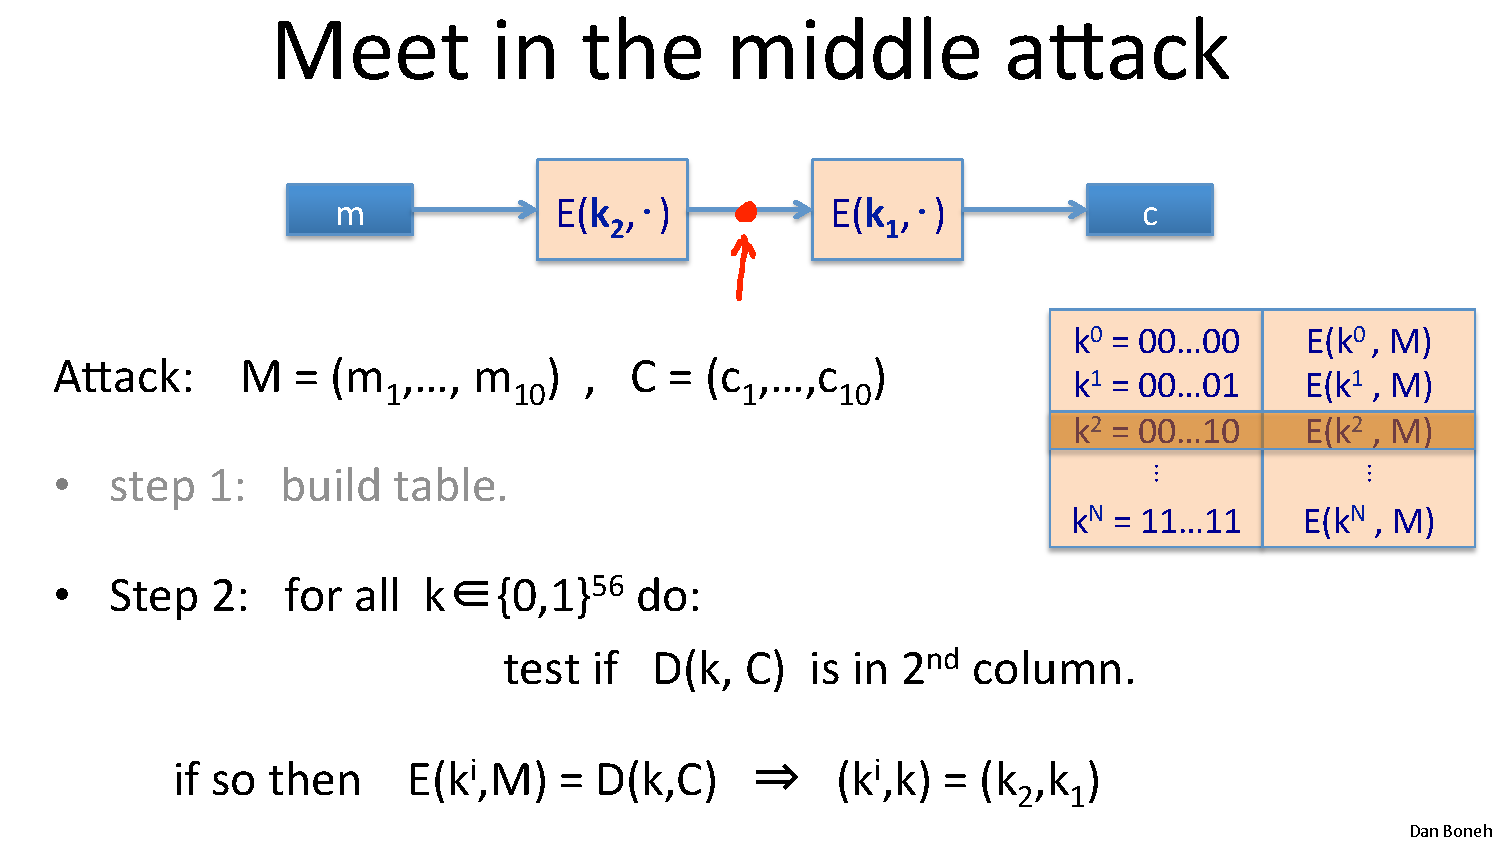
\includegraphics[scale=0.55]{03-block-v2-annotated 35}\\
\captionsetup{labelsep=colon}
\caption{Meet in the middle attack}
\end{figure}
 \paragraph{} So by the way this takes time — to build this table takes time $2^{56}$, and I guess we also want to sort, sorting takes n $\log n$ time, so it's $2^{56}$ times log $2^{56}$. So now that we have this table, we've essentially built all possible values in the forward direction for this point. Now what we're going to do is this meet-in-the-middle attack, where now we try to go in the reverse direction with all possible keys k. Essentially we compute the decryption of c under all possible keys $k_1$. Now for each potential decryption, remember the table holds all possible values in the midpoint, so then for each possible decrpytion, we check, hey, is the decryption in the table, in the second column in the table? If it is in the table, then we found the match, and then what do we know? We know that essentially, well, we found the match, so we know that say for example a decryption using a particular key $k_1$ happened to match this entry in the table, say, $k_2$ or more generally $k_i$, then we know that the encryption of m under $k_i$ is equal to the decryption of c under k. OK, so we kind of build this meet-in-the-middle, where the two sides, you know, the encryption of m under $k_i$ and the decryption of c under k, collided, but if they collided, then we know that in fact this pair, $k_i$ and k, is equal to the pair that we're looking for. And so we've just solved our challenge.
 \paragraph{} So now let's look at what's the running time of this? Well, we had to build a table, and sort it, and then for all possible decryptions, we had to do a search through the table. So there were $2^{56}$ possible decryptions, each search in a sorted table takes $\log(2^{56})$ time, if you just work it out this turns out to be $2^{63}$, which is way, way, way, way, way smaller than $2^{112}$. OK, so this is a serious attack, it's probably doable today, that runs in a total time of $2^{63}$, which is about the same time as the exhaustive search attack on DES. So really, double DES really didn't solve the exhaustive search problem, because, well, there's an attack on it that runs in about the same time as exhaustive search on single DES. Now someone might complain that in fact this algorithm, well, we have to store this big table, so it takes up a lot of space, but you know, so be it. Nevertheless, the running time is still quite small or significantly smaller than $2^{112}$.
 \paragraph{} Now you notice, by the way, this same attack applies to Triple DES. What you would do is you would implement the meet-in-the-middle attack against this point, you would build a table of size $2^{56}$ of all possible encryptions of m, and then you would try to decrypt with all $2^{112}$ keys until you find a collision, and when you find a collision, you have basically found $k_1$, $k_2$, $k_3$. So even Triple DES has an attack that basically explores only $2^{112}$ possible keys. But $2^{112}$ is a large enough number, so Triple DES in fact, as far as we know, is sufficiently secure. I should mention that Triple DES is actually a NIST standard, and so Triple DES is actually used quite a bit, and in fact DES should never ever ever be used, if for some reason you're forced to use some version of DES, use Triple DES, not DES.
 \paragraph{} I want to mention one more method for strengthening DES against exhaustive search attacks. This method actually is not standardized by NIST, because it doesn't defend against more subtle attacks on DES, but nevertheless if all you're worried about is exhaustive search, and you don't want to pay the performance penalties of Triple DES, then this is an interesting idea. So let me show you how it works. So let E be a block cipher that operates on n-bit blocks. We're going to define the EX construction, and for DES we're going to get DESX, to be the following.
\dfn{EX construction(not secure against other kinds of attacks)}{
EX($k_1,k_2,k_3,m$)=$k_1\oplus E(k_2,m\oplus k_3)$
} 
  So we use three keys, $k_1$, $k_2$, $k_3$, and then basically before encrpytion, we XOR with $k_3$, then we encrypt using $k_2$, and then after encryption we XOR with $k_1$. That's it. That's the whole construction. So basically, you'll notice it doesn't slow the block cipher much, because all we did is we applied the cipher plus two additional XORs, which are super fast. The key length for this is in fact, well, we got two keys that are as long as the block size, and we got one key that's as long as the key size, so the total is 184 bits. Now, it turns out actually the best attack that's known is actually an attack that takes time $2^{120}$, and this is actually fairly simple. So it's a generic attack on EX, it will always take time basically block size plus the key size, and it's a simple homework problem for you to try to figure out this attack.
   \paragraph{} In fact there is some analysis to show that there is no exhaustive search attack on this type of construction, so it's a fine construction against exhaustive search, but there are more subtle attacks on DES that we'll talk about in the next part, that basically this construction will not prevent. One thing that I want to point out, unfortunately I found this mistake in a number of products, is if you just decide to XOR on the outside, or if you just decide to XOR on the inside, as opposed to XOR-ing on both sides, which is what DESX does, you notice DESX XORs both on the outside and on the inside, If you just do one of them, then basically this construction does nothing to secure your cipher. It'll still be as vulnerable to exhaustive search as the original block cipher E. So this is another homework problem, and actually you'll see that as part of our homeworks.  So this basically concludes our discussion of exhaustive search attacks, and next we'll talk about more sophisticated attacks on DES.
\subsection{More Attacks on Block Ciphers}
\paragraph{}
There is an immense literature on attacking block ciphers. In this part, I just want to give you a taste for what these attacks look like. And I hope I'll convince you that you should never ever design your own block cipher, and just stick to the standards like Triple DES and AES. The first set of attacks that I want to talk about are attacks on the implementation of the block cipher. As an example, imagine you have a smart card that's implementing a block cipher. So the smart card, for example, could be used for credit card payments. It might have a secret key inside of it to authenticate your credit card payments as you stick the card into a payment terminal, say. So now, if an attacker obtains your smart card, what he could do is he could actually take the smart card to a lab, and then run the card, and measure very precisely how much time the card took to do encryption and decryption. Now, if the amount of time that the implementation took to do encryption depends on bits of the secret key, then by measuring the time, the attacker will learn something about your secret key and in fact, he might be able to completely extract your secret key. And there are many examples of implementations that simply by measuring the time very precisely for many operations of encryption algorithms, you can completely extract the secret key.
\paragraph{} Another example is, rather than just measuring the time, you can actually measure the power consumption of the card as it's operating. So, literally, you can connect it to a device that will measure the current that the card is drawing and then graph the currents very, very precisely. Now, these cards are not very fast, and as a result, you can actually measure the exact amount of power consumed at every clock cycle as the card was executing. When you do that, you actually get graphs of this form. So this is an example of a smart card operating, while it's doing the DES computation. So you can see very clearly, here's when it was doing the initial permutation. Here's when it's doing the final permutation. And then, here, you can count. There are actually sixteen hills and troughs corresponding to the 16 rounds. And essentially when you zoom in on a graph like this, you can basically read the key bits off one by one, just by looking at how much power the card consumed as it was doing the different operations. It turns out that, even cards that take steps to mask this type of information, are still vulnerable. There's an attack called differential power analysis, where basically, you measure the power consumed by the card over many, many runs of the encryption algorithm. And as long as there's any even small dependence between the amount of current consumed and the bits of the secret key, basically that dependence will show up after enough runs of the encryption algorithm. And as a result you'll be able to completely extract the secret key.
\paragraph{} These attacks were actually discovered by Paul Kocher and his colleagues up at Cryptography Research and there's actually a fairly large industry devoted to just defending against these power attacks. As far as timing attacks are concerned, I want to mention that these are real. They're not just about smart cards. For example, you can imagine a multicore processor where the encryption algorithm is running on one core and the attacker code happens to be running on another core. Now these cores actually share the same cache. And as a result, an attacker can actually measure or can actually look at the exact cache misses that the encryption algorithm incurred. It turns out that by looking at cache misses, you can completely figure out the secret key used by the algorithms. So, one core can essentially extract information from the other core, just by looking at cache misses.
\paragraph{} So implementing these block ciphers is actually quite subtle because you have to make sure that the side channel attacks don't leak information about your secret key. Another type of attack that's been discussed in the literature is what's called a fault attack. So here, basically, if you're attacking a smart card, you can actually cause the smart card to malfunction, perhaps by overclocking it, perhaps by warming it up. Essentially, you can cause the processor to, malfunction, and output erroneous data. It turns out that, if, during encryption, there are errors in the last round of the encryption process, the resulting ciphertexts that are produced are enough to actually expose the secret key K. That's quite an interesting result that in fact if you have any errors, if you ever output a wrong result, that actually could completely compromise your secret key. So, of course, the defense against this means that before you output the result of your algorithm, you should check to make sure that the correct result was computed. Now of course that's nontrivial, because how do you know that the error didn't happen in your checking algorithm. But there are known ways around that. So basically you can actually compute something three or four times, take the majority over all those results, and be assured that the output really is correct as long as not too many faults occurred inside of your computation.
\paragraph{} These are attacks on the implementation. I hope these examples can assure you that not only should you not invent your own block ciphers, you should never even implement these crypto primitives yourself. Because A : you have to make sure there are no side channel attachments on your implementation and B :  you have to make sure that the implementation is secure against fault attacks. So, instead you should just use standard libraries like the ones available in \underline{OpenSSL} and many other libraries out there. So don't implement these primitives yourself, just use existing libraries.
\paragraph{} All right, so now I want to turn to kind of more sophisticated attacks on block ciphers and I'll particularly talk about how these attacks apply to DES. These attacks were discovered by \underline{Biham and Shamir back in 1989}, and I'll particularly describe a version of the attack discovered by \underline{Matsui in 1993}. So the goal here is basically given many input-output pairs, can we actually recover the key better than exhaustive search? So anything that runs better than exhaustive search already counts as an attack on the block cipher. So the example I want to give you is what's called linear crypto analysis.

\begin{figure}[H]
\centering
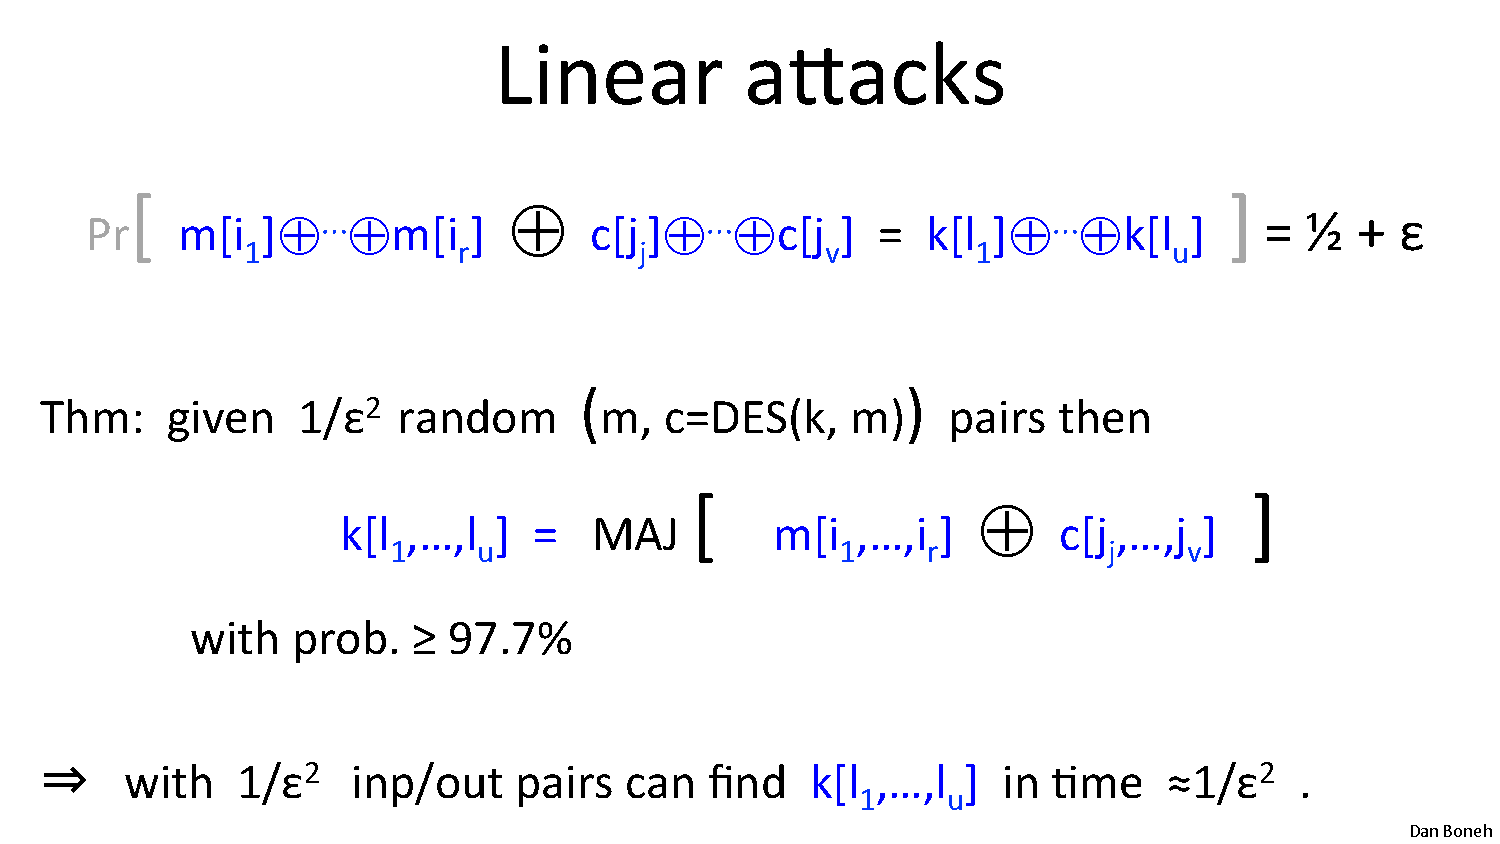
\includegraphics[scale=0.55]{03-block-v2-annotated 42}\\
%\captionsetup{labelsep=colon}
\caption{}
\end{figure}
\paragraph{}
 And here imagine it so happens that, you know, c is the encryption of m using key k, and suppose it so happens that if I look at random key and a random message, somehow there's a dependence between the message, ciphertext, and the key bits. In particular, if I XOR a subset of the message bits, so this is just a subset of the message bits, if I XOR that with a certain subset of the ciphertext bits. The attacker has the message and the attacker has the ciphertext. And then you compare that to an XOR of a subset of the key bits.
 \paragraph{} Now if the two were completely independent which is what you'd like, you definitely don't want your message and your ciphertext to somehow predict your key bits, if the two are like, completely independent, then this equality will hold with probability exactly $\frac{1}{2} $. But suppose it so happens that there's a bias and this probability holds with probability $ \frac{1}{2} + \epsilon$. It so happens that, in fact, for DES, there is such a relation. The relation holds specifically because of a bug in the design of the fifth S-box. It turns out the fifth S-box happens to be too close to a linear function. And that linear function, basically, as it propagates through the entire DES circuit, generates a relation of this type. You notice, this is basically a linear relation that's being computed here. So, this small tiny linearity in the fifth S-box generates this relation over the entire circuit, where the epsilon is tiny. Epsilon is one over $2^{21}$, and I wrote down what that is. So the bias is really small. But nevertheless, there is a bias using these particular subsets of bits.
 \paragraph{} Now, I'm not going to show you how to derive this relation, or I'm not going to show you even what it is. I'll just tell you how to use a relation like this once you find it. Okay. So here's our relation that we have. And the question is how to use it. So with a little bit of statistics you can actually use an equation like this to determine some of the key bits. And here's you do it. Suppose you were given one over epsilon squared message-ciphertext pairs. And these have to be independently random messages and the corresponding ciphertexts. What you would do is you would use the formula above. In fact you would use the left-hand side of the formula above to compute this relation between the message and ciphertext for all the pairs you were given. You know that for $ \frac{1}{2} + \epsilon$ of these values, you know that these things will be equal to an XOR of the key bits. So if you take majority over all the values you've computed, it turns out it's not so difficult to see that in fact you'll get the correct prediction for the XOR of the key bits with a probability of 97.7\%. In other words, if this relation happens to be correct more than half the time, then the majority will be right. And because there's a bias, there's an epsilon bias, the probability that you will be correct more than half the time is, in fact, 97.7\%. In which case, the majority, in fact, will give you the correct XOR of the key bits. 
 \paragraph{} So this is kinda cool. Within one over epsilon squared time, you can figure out an XOR of a bunch of key bits. So now, let's apply this to DES. So, for DES, we have epsilon, which is one over $2^{21}$. Which means that if you give me $2^{42}$ input-output pairs, I can figure out an XOR of the key bits. And now, it turns out, I'm not going to exactly show you how, roughly speaking, using this method, you don't just get one key bit. In fact, you get two key bits. You can kind of use this relation. One's going in a forward direction and one's going in a backwards direction. So that gives you two XORs of bits of the secret key. So that's two bits of information about the secret key. And then it turns out you can get twelve more bits, because, essentially, you can figure out what the inputs are to the fifth S-box.
 \paragraph{} Okay, so, I'm not going to exactly show you how. But it turns out you can get 12 more bits, which is a total of 14 bits overall. So now, using this method, you've recovered fourteen bits of the secret key. And of course, it took you time $2^{42}$. Okay, so then, what do you do? Well, so the rest of it is easy. Now what you're going to do is you're going to do exhaustive search on the remaining bits. Well how many remaining bits are there? Well, there are 42 remaining bits, so the exhaustive search will take you time $2^{42}$. So what's the total attack time? Well, the first step of the algorithm to determine the fourteen bits took $2^{42}$ time, and the remaining brute force search also took $2^{42}$ time. So overall, the attack took $2^{43}$ time. So now, this is much better than exhaustive search. Within $2^{43}$ time, we broke DES. But of course, this required $2^{42}$  random input-output pairs whereas exhaustive search only required three pairs.  So this is a fairly large number of input-output pairs that are needed, but given such a large number, you can actually recover the key faster than exhaustive search.
 \begin{note}
 \paragraph{} \textbf{What's the lesson in all this?} The lesson is, \textbf{firstly}, any tiny bit of linearity, basically, in this— in the fifth S-box, which was not designed as well as the other S-boxes, basically led to an attack on the algorithm. A tiny bit of linearity already introduced this linear attack. And I want to emphasize again that this is not the sort of thing you would think of when you design a cipher. And so again, the conclusion here is, there are very subtle attacks on block ciphers, ones which you will not be able to find yourself. And so just stick to the standards. Don't ever, ever, ever design your block cipher.
 \paragraph{} Okay, so that's all I want to say about sophisticated attacks. Now let's move on to the last type of attack that I want to mention, which I'll call \textbf{quantum attacks}, which are are generic attacks on all block ciphers. So let me explain what I mean by this. So first of all, let's look at a generic problem, a generic search problem. Suppose I have a function on some large domain X, that happens to be two outputs, either zero or one. And it so happens that this function is mostly zero. And there's, like, maybe one input where the function happens to evaluate to one. And your goal is basically, you know, find me the inputs where the function happens to be one. Maybe there's only one such input. But your goal is to find it. Well, so on a classical computer, what can you do? The function is given to you. It's given to you as a black box. So the best you can do is just try all possible inputs. So this is going to take time which in linear in the size of the domain.
 \paragraph{} Now, it turns out there's an absolutely magical result that says that if you build a computer that's based on quantum physics as opposed to classical physics, you can solve this problem faster. So let me explain what I mean by this. So first of all in the 70s and 80s it was observed, I think it was actually Richard Feynman who observed this initially, that said that it turns out to be very difficult to simulate quantum experiments on a classical computer. So Feynman said, if that's the case, maybe these quantum experiments are computing things that a classical computer can't compute. So they're somehow able to compute very quickly things that are very difficult to do classically. And that turned out to be correct.
 \paragraph{} And in fact, the example I want to show you is one of these amazing things that in fact, if you could build a quantum computer that's using quantum physics, then it's, in fact, you can solve this search problem not in time X but in time $\sqrt{|X|}$. So somehow, even though the computer doesn't know anything about the function F, it's treating it as a black box, nevertheless, it's able to find a point where the function is one, in time $\sqrt{|X|}$. It's actually quite interesting, and, in fact, quantum computers have quite an impact on crypto.
 \paragraph{} \textbf{So what does this have to do with breaking block ciphers?} So far it's just a generic search problem. Well, oh actually I should say before I show you the application, I should mention that, well, you might be wondering, well, can someone build a quantum computer. And this is still completely unknown. At this point, nobody really knows if we can build large enough quantum computers to actually take advantage of this beautiful algorithm due to Grover. Alright, so \textbf{what does this have to do with block ciphers?} Well, so suppose I give you a message-ciphertext pair. Just one or just a few. We can define a function as follows. It's a function on K, it's a function on, the key space. And the function will basically output one if it so happens that the encryption of m with k maps to c, and it will output zero otherwise. Now we argue that basically this is exactly the type of function that's one at one point in the key space and that's it.
 \paragraph{} So by \textbf{Grover's algorithm}, we can actually find the secret key in time square root of K. So what does that mean? For DES, this would totally destroy DES. This would say that in time $2^{28}$, you could find a key. $2^{28}$ is about 200 million. So 200 million steps which is, you know, just takes a millisecond on a modern computer. This would totally destroy DES. But even AES with 128-bit keys, you would be able to find the secret key in time, roughly $2^{64}$. And $2^{64}$ is these days, considered insecure. That's within the realm of exhaustive search.
 \paragraph{} Basically, if somebody was able to build a quantum computer, we would then say that AES-128 is no longer secure. Instead, if somebody, you know, if tomorrow, you open up the newspaper, and you read an article that says, you know, so-and-so built a quantum computer, the conclusion, the consequence of all that is that you should immediately move to block ciphers that use 256 bits, because then the running time of Grover's algorithm is $2^{128}$, which is more time than we consider feasible, and the, basically there are example ciphers with 256 bits, for example, AES-256. This is one of the reasons why AES was designed with 256 bits in mind. But to be honest, this is not the only reason. There are other reasons why you want it to have larger key sizes. 
 \end{note}

\section{Block Ciphers 3: AES and other constructions}
\subsection{The AES Block Cipher}
\paragraph{}
Over the years it became clear that DES and triple DES are simply not designed for modern hardware and are too slow. As a result, NIS started a new process to standardize in a new block cipher called the Advanced Encryption Standard or AES for short. Nis started it's effort in 1997 when it requested, proposals for a new block cipher. It received fifteen submissions a year later. And finally in the year 2000, it adopted the cipher called Rindall as the advanced encryption standard. This was a cipher designed in Belgium. We already said that it's block size is 128 bits and it has three possible key sizes. 128 bits, 192, and 256. Now, the assumption is that the larger the key size is, the more secure the block cipher is as a pseudo random permutation. But because it also has more rounds involved in its operation. The slower the cipher becomes. So the larger the key supposedly, the more secure the cipher, but also the slower it becomes. So for example, AES 128 is the fastest of these ciphers and AES 256 is the slowest.
\paragraph{} Now AES is built as what's called a substitution permutation network. It's not a Feistel network. Remember that in a Feistel network, half the bit were unchanged from round to round. In a substitution permutation network all the bits are changed in every round. And the network works as follows, so here we have the first round of the substitution permutation network, where the first thing we do is we XOR the current state with the round key. In this case the first round key. Then we go through a substitution layer, where blocks of Date are replaced with other blocks based on what the substitution table says. And then we go through a permutation layer where bits are permuted and shuffled around. And then we do this again.
\begin{figure}[H]
\centering
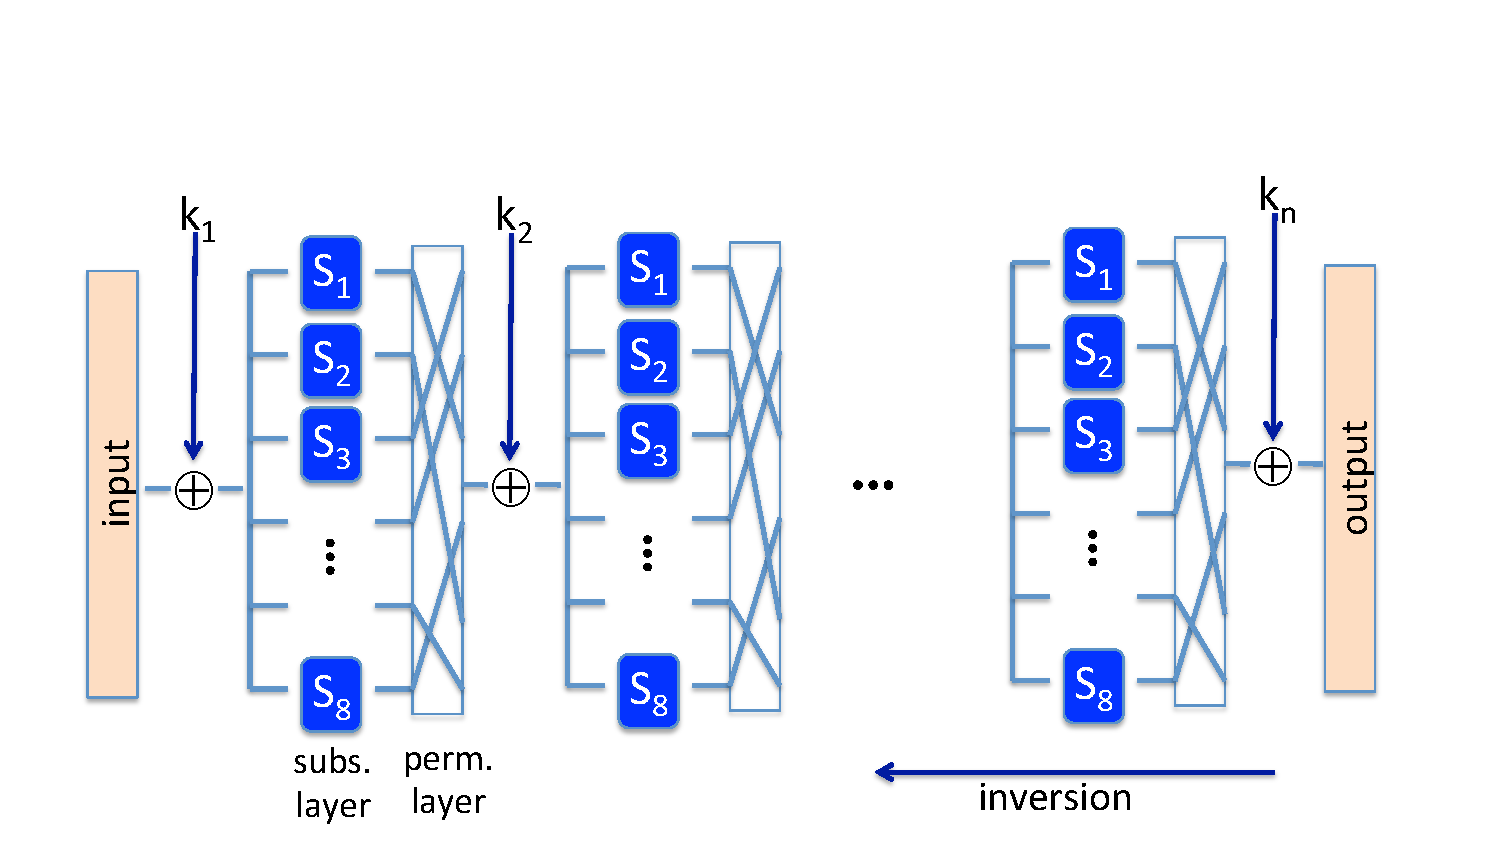
\includegraphics[scale=0.55]{03-block-v2-annotated 50}\\
\captionsetup{labelsep=colon}
\caption{AES}
\end{figure}
\paragraph{}
 We XOR with a round key, we go through a substitution phase, and we're permute to dance around. And so on, and so on, and so forth Until we reach the final round where we XOR with the very last around key, and then out comes the output. Now, and important point about this design. Is that, in fact, because of how it's built, every step in this network needs to be reversible, so that the whole thing is reversible. And so the way we would, decrypt, essentially, is we would take the output and simply apply each step of the network in reverse order. So we start with the permutation step, and we have to make sure that step is reversible. Then we look at the substitution layer, and we have to make sure this step is reversible.
 \paragraph{} And this is very different from DES. In DES, if you remember, the substitution tables were not reversible at all. In fact, they map six bits to four bits. Whereas here, everything has to be reversible, otherwise it would be impossible to decrypt. And of course the x or with the round key is reversible as well. So inversion of a substitution permutation network is simply done by applying all of the steps in the reverse order. So now that we understand the generic construction.
 \paragraph{} Lets look at the specifics of AES. So AES operates on a 128 bit block. Which is 16 bytes. So what we do with AES is we write those 16 bytes as a four by four matrix. Each cell in the matrix contains one byte. And then we start with the first round so we XOR with the first round key and then apply a certain function. That, includes substitutions and permutations and other operations on the state. And again, these three functions that are applied here have to be invertible so that in fact the cipher can be decrypted. And then we xor with the next round key and we do that again. Again we apply the round function and xor the round key. And we do that again and again. We do it ten times. Although interestingly in the last round, the mix column step is actually missing. And then finally, we XOR with the last rounds key, and out comes the output.
\begin{figure}[H]
\centering
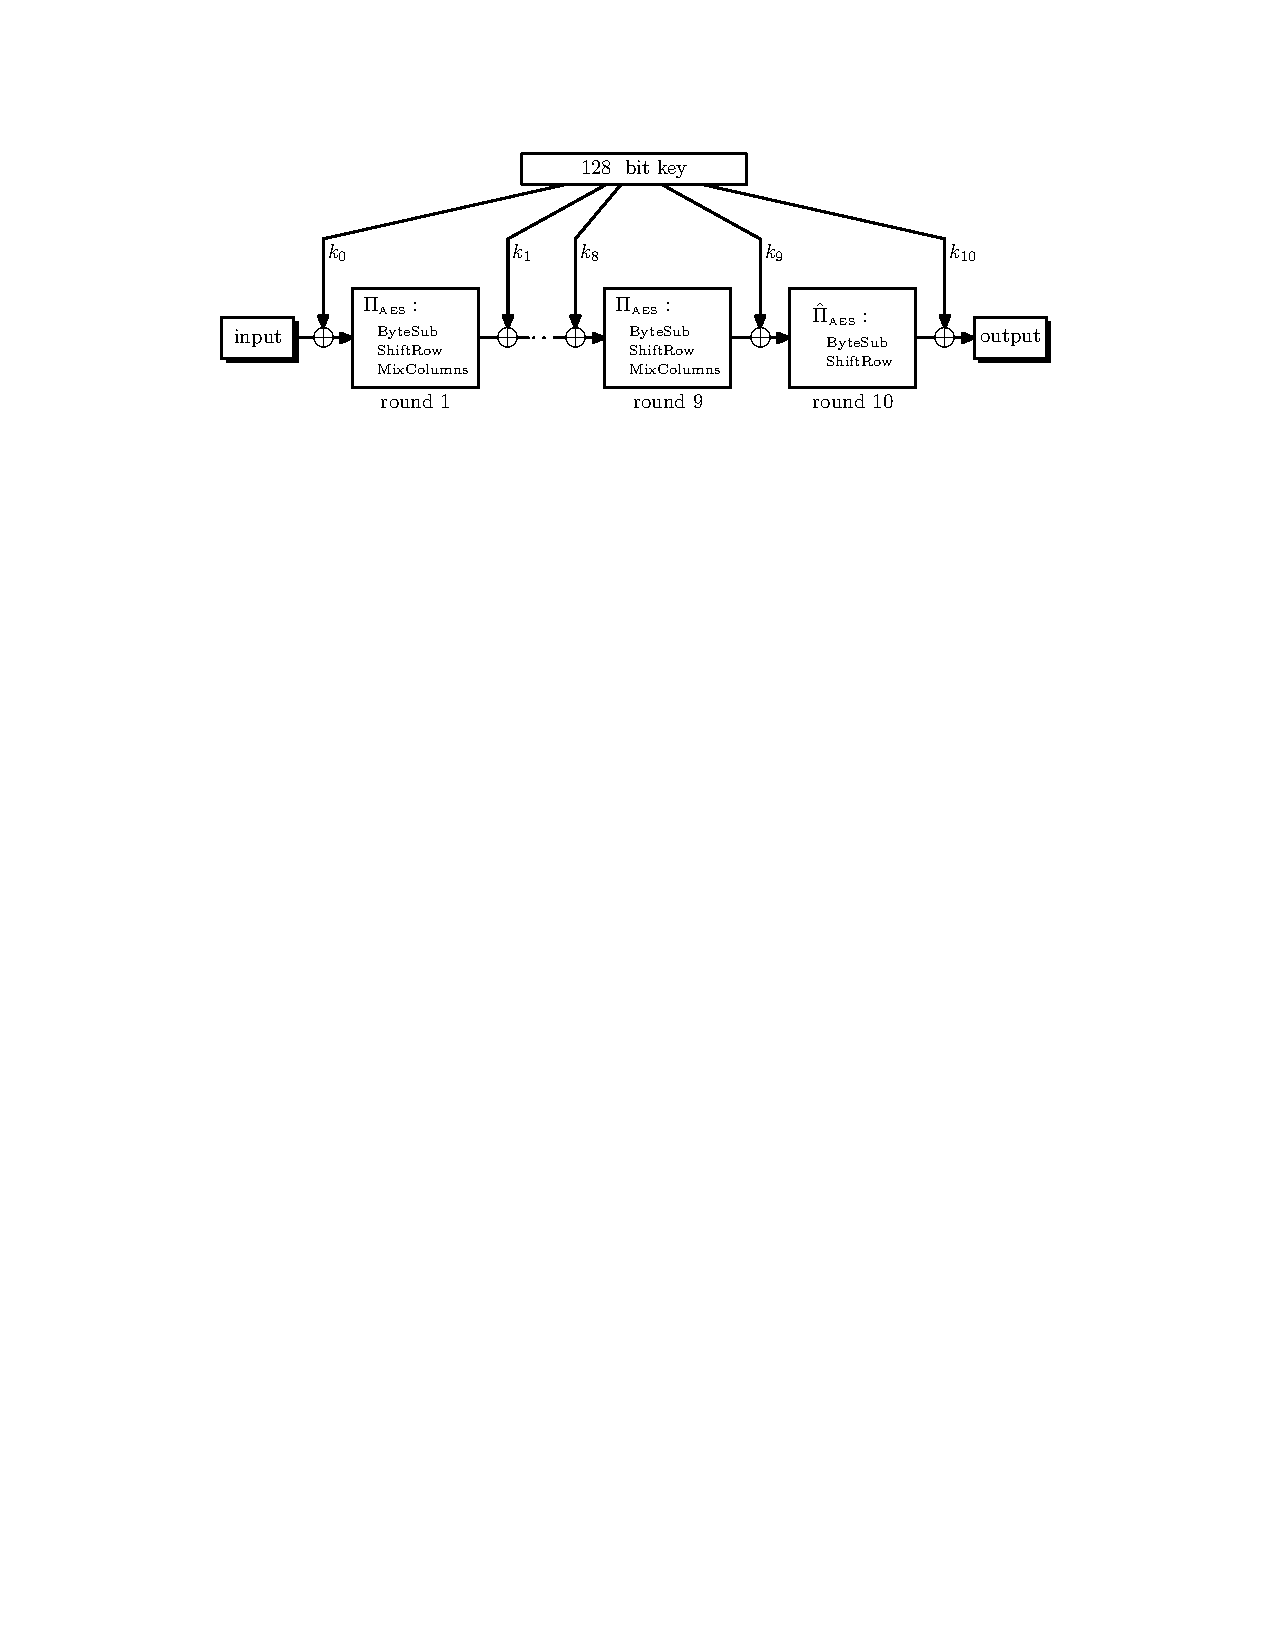
\includegraphics[scale=0.65]{crypto boneh book draft 134}\\
\captionsetup{labelsep=colon}
\caption{AES-128 schematic}
\end{figure} 
 \paragraph{} Again, in every phase here, we always, always keep this four by four array. And so the output is also four by four, which is 16 bytes, which is 128 bits. Now the long key themselves of course come from a 16 byte AS key using key expansion. So the key expansion maps from a sixteen bytes AS key into eleven keys, each one being 16 bytes. So these keys themselves are also a four by four array that's XORed into the current state. Okay, so that's the schematic of how AES works. And the only thing that's left to do is specify these three functions, byte sub, shift row, and mixed column. And those are fairly easy to explain. So I'm just going to give you the high level description of what they are. And, those interested in the details can look it up online.
 \paragraph{} So the way byte substitution works, is literally it's one S box containing 256 bytes. And essentially, what it does is it applies the S box to every byte in the current states. So, let me explain what I mean by that. So the current state is going to be this four by four, table. So here we have the four by four table. And to each element in this table, we apply the S box. So let's call it the A table. And then what we do is, essentially, for all four by four entries, essentially, the next step, Aij. Becomes the current step evaluated at the look up table. So we use the current cell as an entry, as an index, into the look up table. And then the value of the look up table is what's output.
 \paragraph{} So, that's the first step. The next step that happens is a shift step, which is basically just a permutation. So essentially we kind of do a cyclic shift on each one of the rows. So you can see the second row is cyclically shifted by one position. This third row is cyclically shifted by two positions and the third row is cyclically shifted by three positions.
\[
\begin{bmatrix}
a_0 & a_1 & a_2 & a_3 \\
a_4 & a_5 & a_6 & a_7 \\
a_8 & a_{9} & a_{10} & a_{11}\\
a_{12} & a_{13} & a_{14} & a_{15} 
\end{bmatrix}
\rightarrow
\begin{bmatrix}
a_0 & a_1 & a_2 & a_3 \\
a_5 & a_6 & a_7 & a_4 \\
a_{10} & a_{11} & a_8 & a_{9}   \\
a_{15} & a_{12} & a_{13} & a_{14}  
\end{bmatrix}
\] 
  And the last thing we do is mix columns where literally we apply a linear transformation to each one of these columns. So there's a certain matrix that multiplies each one of these columns and it becomes, the next column. So these linear transformation is applied independently to each one of the columns. Now, I should point out that, so far, shift rows and mixed columns are very easy to implement in code. And I should say that the transformation itself is also easily computable, so that you can actually write code that takes less than 256 bytes to write.
  \paragraph{} You can kind of shrink the description of AES by literally storing code that computes the table rather than hardwiring the table into your implementation. And in fact, this is kind of a generic fact about AES, that if you can have allowed no pre-computation at all, including computing the S box on the fly. Then in fact you get a fairly small implementation of AES, so it could fit on very constrained environments where there isn't enough room to hold, complicated code. But of course, this will be the slowest implementation, because everything is computed now on the fly, and as a result, the implementation, obviously, is going to be, slower than things that were pre-computed.
  \paragraph{} And then there is this trade off. For example if you have a lot of space, and you can support large code. You can actually pre-compute quite a bit of the three steps that I just mentioned. In fact, there are multiple options of pre-computation, you can build a table that's only four kilobyte big. You can build a table that is even longer, maybe 24 kilobytes. So basically you will have these big tables in your implementation. But then your actual performance is going to be really good, because all your doing is just table look-ups and XORs. You're not doing any other complicated arithmetic. And as a result, if you can do a lot of pre-computation, these three steps here, you should. Sbox and mixed columns can be converted just into a number, a small number of table lookups and. All you can do is just compute the S box, so now your implementation would just have 256 bytes Hard coded .The rest would just be code that's actually computing these three functions. The performance would be slower than in the previous step but the code footprint would also be smaller.
  \paragraph{} Overall, there's this nice tradeoff between code \textbf{size} and \textbf{performance}. So on high-end machines, on high-end servers, where you can afford to have a lot of code, you can precompute and store these big tables and get the best performance. Whereas on low-end machines like eight byte smart cards or think of like an eight byte wristwatch, you would actually have a relatively small implementation of AES. But as a result of lecture it won't be so fast. So here's an example that's a little unusual, suppose you wanted to implement AES in Javascript so you can send an AES library to the browser and have the browser actually do AES by itself.
  \paragraph{} So in this case what you'd like to, to is you'd like to both shrink the code size, so that on the network there's minimum traffic to send a library over to the browser but, at the same time, you'd like the browser performance to be as fast as possible. And so this is something that we did a while ago essentially the idea is that the code that actually gets send to the browser doesn't have any pre computed table and as a result is fairly small code. But then the minute it lands on the browser, what the browser will do is actually pre compute all the tables. So in some sense the code goes from just being small and compact. It gets bloated with all these precomputed tables. But those are stored on the laptop, which presumably has a lot of memory. And then once you have the precomputed tables you actually encrypt using them. And that's how you get the best performance. 
  \paragraph{} So if you have to stand in implementation AES over the network, you can kind of get the best of all worlds. Whereas, the code over the network is small, but when it reaches the target client, it can kind of inflate itself. And then get the best performance as it's doing encryption on the clients. Now AES is such a popular block cipher, now essentially when you build crypto into products essentially your supposed to be using AES, and as a result Intel actually put AES support into the processor itself.
  \paragraph{} So since there are special instructions in the Intel processor to help accelerate AES. And so I listed these instructions here. They come in two pairs, aesenc and aesenclast. And then, there's aesekygenassist. So, let me explain what they do. So, aesenc essentially implements one round of AES. Namely, apply the three functions in the XOR with the round key. And aesenclast basically implements the last round of AES. Remember, the last round didn't have the mix columns phase. It only had the subs bytes and shift rows. And so that's why the aesenclast does. And the way you call these instructions is using 128 byte registers which correspond to the states of AES. And so you would have one register containing the states and one register containing the current round key. And then when you call AES on these two registers, basically, they would run one round of AES and place the result inside of this XMM one state register. And as a result if you wanted to implement the whole AES. All you would do is, call aesenc nine times. Then you would call aesenclast one time. These ten instructions are basically the entire implementation of AES.
  \paragraph{} It's that easy to implement AES on this hardware and they claim because these operations are now done inside the processor not using external instructions that are implemented in the processor. They claim that they can get a fourteen X speedup over say an implementation that's running in the same hardware but implementing AES without these special instructions. So this is quite a significant speed up and the facts are now lots of. Products that make use of these special instructions. And let's just say that this is not specific to Intel, if you're in AMD, and they also implemented similar instructions in their Bulldozer architecture and further and future architectures.
  \paragraph{} Let's talk about the security of AES. I want to mention just two attacks here. Obviously, AES has been studied quite a bit. But the only two attacks on the full AES are the following two. So, \textbf{first of all}, if you wanted to do key recovery, the best attack, basically, is only four times faster than exhaustive search. Which mean that instead of a hundred and. 28 bits key, really you should be thinking of AES. Is 126 bit key. Because exhaustive search, really it's going to four times faster than it should. Of course due to the 126, is still more time than we have to compute, and this really does not hurt the security alias. The more significant attack is, actually, on AES-256. It turns out there's a weakness in the key expansion design of AES which allows for, what's called a related key attack.
  \paragraph{} So, \textbf{what's a related key attack?} Essentially, if you give me about $2^{100}$  input output pairs for AES, but from four related keys. So, these are keys that are very closely related, namely key number one. Is just one bit flip of key \# four, which is just one flip, bit flip of key \# three, which is just one flip bit flip of key \#four. These are very closely related keys, if you like your distances very short. But if you do that, then, in fact, there is a $2^{100}$ attack. Now you should say, well, $2^{100}$ is still impractical. This is still more time than we can actually run today. But nevertheless, the fact that it's so much better than an exhaustive search attack, it's so much better than $2^{256}$, is kind of a limitation of the cipher. But generally, it's not a significant limitation, because it requires related keys. And so, in practice, of course, you're supposed to be choosing your keys at random, so that you have no related keys in your system. And as a result, this attack wouldn't apply. But if you do have related keys, then there's a problem. In the next part we're going to talk about more provably secure constructions for block ciphers.
\subsection{Block Ciphers From PRGs}
\paragraph{}
In this part we ask whether we can build block ciphers from simpler primitives like pseudo random generators. The answer is \underline{yes}. So to begin with, let's ask whether we can build pseudo random functions as opposed to pseudo random permutations from a pseudo random generator. Can we build a PRF from a PRG? Our ultimate goal though is to build a block cipher which is a PRP. And we'll get to that at the end. For now we build a PRF. So let's start with a PRG that doubles its inputs so the seeds for the PRG is an element in K and the output is actually two elements in K. And now what does it mean for this PRF to be secure, recall this means that essentially the output is indistinguishable from a random element inside of $\mathcal{K}^2$ Now it turns out that it's very easy to define basically what's called a one-bit PRF from this PRG.
\paragraph{} So what's a one bit PRF is basically a PRF who's domain is only one bit. So it's a PRF that just takes one bit as input. And the way we'll do it is we'll say is if the input bit X is zero I'll put the left output and if the input bit X is one then I'll put the right output of the PRF. In symbols we basically have what we wrote here. Now it is straightforward to show, that in fact G is a secure PRG, then this one bit PRF is in fact a secure PRF. It's really just stating the same thing twice. So i will leave it for you to think about this briefly and see and convince yourself that in fact this theorem is true.
\paragraph{} The real question is whether we can build a PRF, that actually has a domain that is bigger than one bit. Ideally we would like the domain to be 128 bits, just say as AES has. So the question is can we build 128 bit PRS from a pseudo random generator. Well so let's see if we can make progress. So the first thing we're going to do is we're going to say, well again, let's start with a PRG that doubles its input let's see if we can build a PRG that quadruples its inputs. So it goes from K to K to the fourth instead of K to K squared. So let's see how to do this. So here we start with our original PRG that just doubles its inputs, now remember that the fact that his is a PRG means that the output of the PRG is indistinguishable from two random values in K. Well, if the output looks like two random values in K, we can simply apply the generator again to those two outputs. So let's say we apply the generator once to the left output, and once to the rights outputs. And we are going to call the output of that, this quadruple of elements, $G_1(k)$. So now that we have a generator from K to $\mathcal{K}^4$, We actually get a two bit PRF. Namely, what we will do is, we will say, given two bits, 00,01,10 or 11, will simply output the appropriate block that the output of $G_1(k)$. Okay, so now we can basically have a PRF that takes four possible inputs as opposed to just two possible inputs as before.
\dfn{Tree construction PRF from PRG}{For $x=(a_1\ldots a_n)\quad a_i \in \{0,1\}$ and a PRG that doubles its input length $G(k)=(G_0(k),G_1(k))$ we have:
\begin{algorithm}[H]
\KwIn{$k\in \mathcal{K}\quad x\in \{0,1\}^n$}
\KwOut{$t\in \mathcal{K}$}
\SetAlgoLined
\SetNoFillComment
\vspace{3mm}
t=k\;
\For{$i$ in $1,\ldots ,n$} {
    $t=G_{a_i}(k)$\;
}
\Return t\;
\caption{what}
\end{algorithm}
}
\begin{figure}[H]
\centering
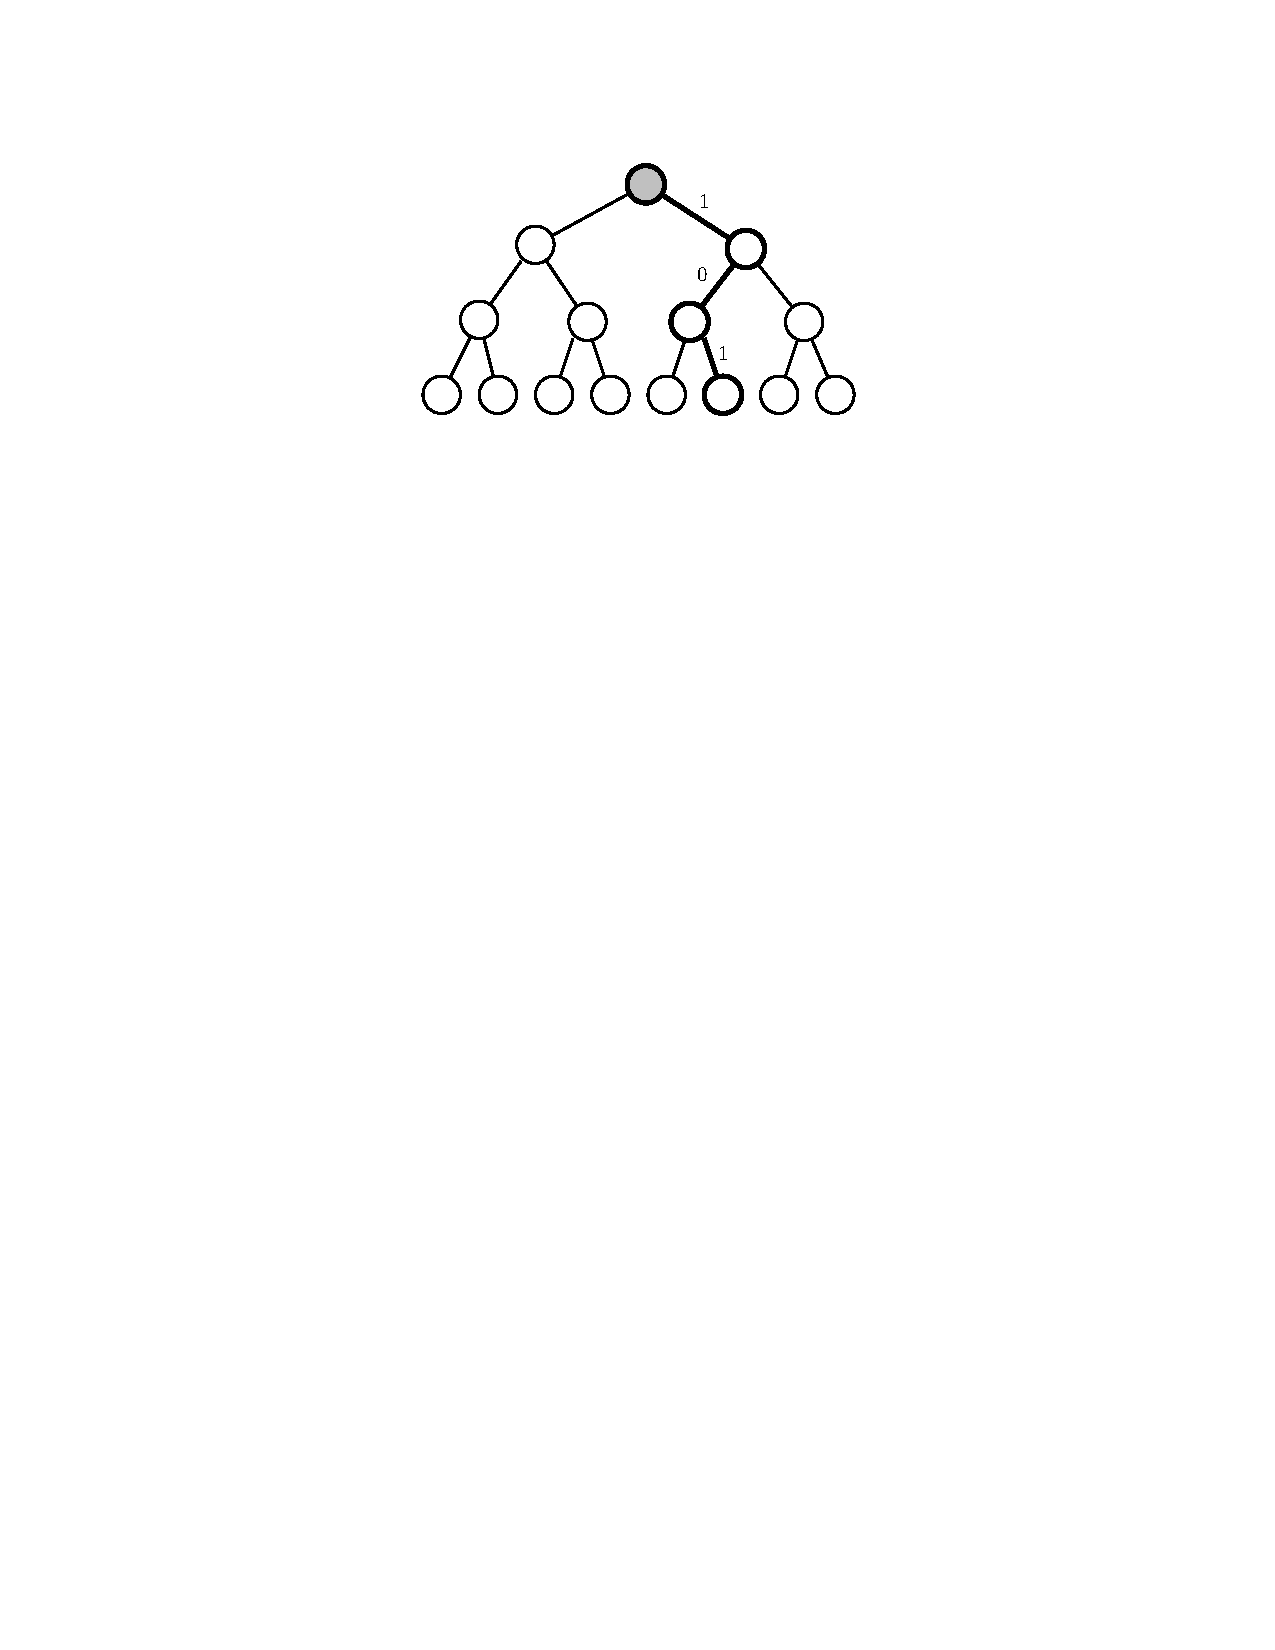
\includegraphics[scale=0.65]{crypto boneh book draft 164}\\
\captionsetup{labelsep=colon}
\caption{Diagram for a three-bit input}
\end{figure} 
\thm{Security of the tree construction}{If the PRG is secure, then the resulting PRF will also be secure}
\paragraph{} So the question you should be asking me is why is this $G_1$ case secure? Why is it a secure PRG? That is why is this quadruple of outputs indistinguishable from random. And so let's do a quick proof of this, we'll just do a simple proof by pictures. So here's our generator that we want to prove is secure. And what that means is that we want to argue that this distribution is indistinguishable from a random fordable in K to the fourth. So our goal is to prove that these two are indistinguishable.
\begin{figure}[H]
\centering
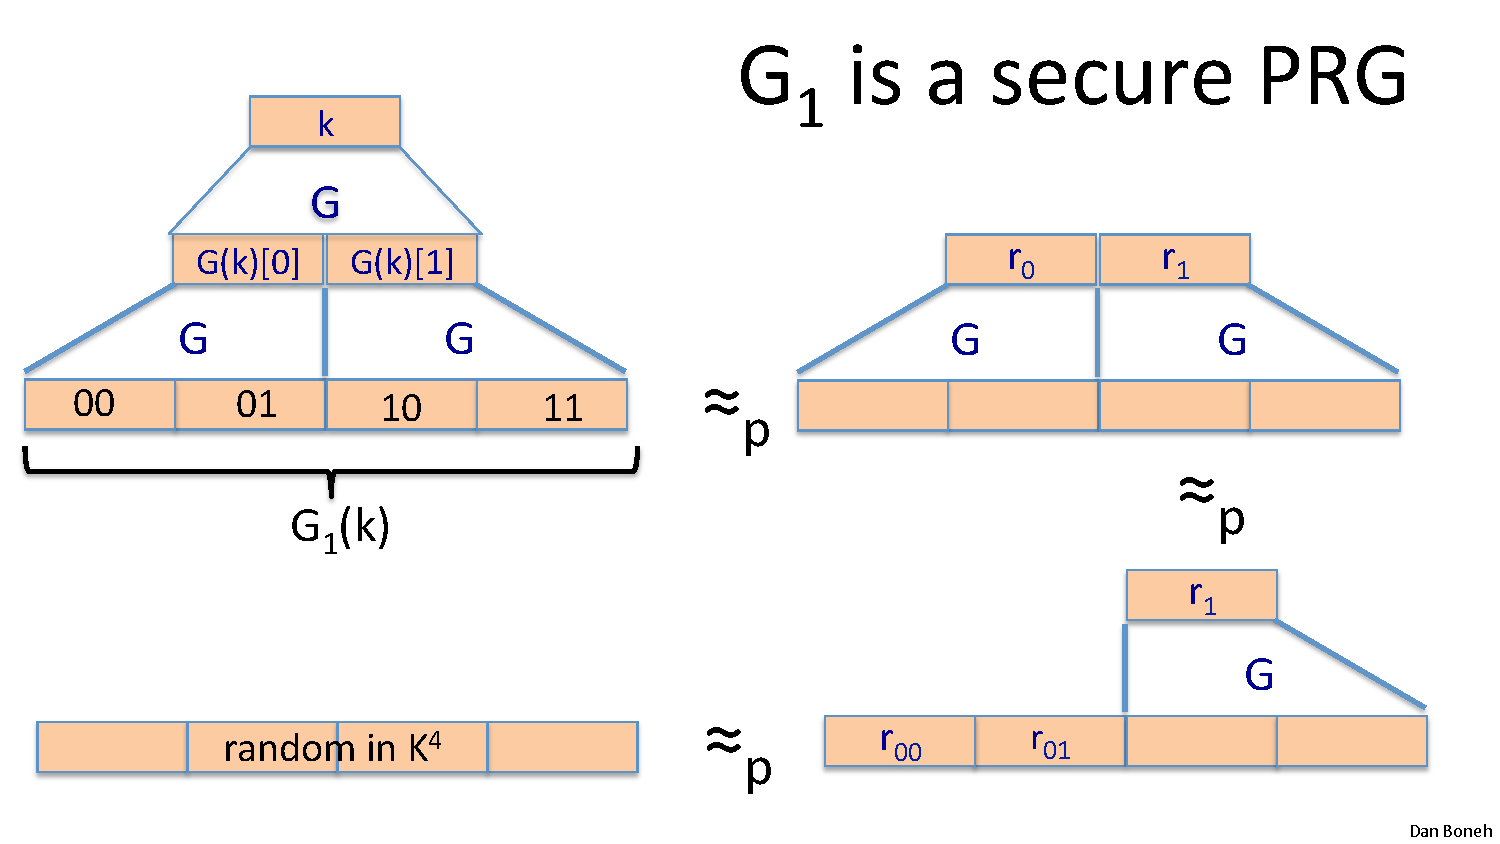
\includegraphics[scale=0.45]{03-block-v2-annotated 61}\\
\captionsetup{labelsep=colon}
\caption{Proof by pictures}
\end{figure}
\paragraph{}
 Well let's do it one step at a time. We know that the generator is a secure generator, therefore in fact the output of the first level is indistinguishable from random. In other words, if we replace the first level by truly random strings these two are truly random picked in the key space, then noefficient adversary should be able to distinguish these two distributions. In fact, if you could distinguish these two distributions, it's easy to show that you would break the original PRG. But essentially you see that the reason we can do this replacement, we can replace the output of G, with truly random values, is exactly because of the definition of the PRG, which says the out put of the PRG is indistinguishable from random, so we might as well just put random there, and no efficient adversary can distinguish the resulting two distributions. 
\paragraph{} So far so good, but now we can do the same thing again to the left hand side. In other words, we can replace these two pseudo random outputs, by \textbf{truly random outputs}. And again because the generator G is secure, no efficient adversary can tell the difference between these two distributions. But differently, if an adversary can distinguish these two distributions, then we would also give an attack on the generator G. And now finally we're going to do this one last time. We're going to replace this pseudo random pair By a truly random pair, and we get the actual distribution that we were shooting for, we would get a distribution that is really made of four independent blocks.
\paragraph{} And so now we have proved this transition basically that these two indistinguishable, these two indistinguishable, and these two indistinguishable, and therefore these two are indistinguishable, which is what we wanted to prove. This is kind of the high level idea for the proof, it is not too difficult to make this rigorous, but i just wanted to show you kinda intuition for how the proof works. Well, if we were able to extend the generators outputs once, there's nothing preventing us from doing it again so here is a generator $G_1$ that outputs four elements in the key space. And remember the output here is indistinguishable from our random four couple, that's what we just proved.
\paragraph{} And so there's nothing preventing us from applying the generator again. So we'll take the generator apply it to this random looking thing and we should be able to get this random looking thing. This pair over here that's random looking. And we can do the same thing again, and again, . And now basically we've built a new generator that outputs elements in K to the eighth, as opposed to K to the fourth. And again the proof of security is very much the same as the one I just showed you essentially you gradually change the outputs into truly random outputs. So we would change this to a truly random output, then this, then that, then this, then that and so on and so forth. Until finally we get something that's truly random and therefore the original two distributions we started with $G_{2}(k)$ and truly random are indistinguishable. So far so good. So now we have a generator that outputs elements in $\mathcal{K}^8$. Now if we do that basically we get a three bit PRF.
 \paragraph{} Now the interesting thing is that in fact this PRF is easy to compute. For example, suppose we wanted to compute the PRF at the point 101. It's a three bit PRF.  How would we do that? Well basically we would start from the original key K. And now we would apply the generator G but we would only pay attention to the right output of G, because the first bit is one. And then we will apply the generator again, but we would only pay attention to the left of the output of the generator because the second bit is zero. And then we would apply the generator again and only pay attention to the right outputs because the third bit is one and that would be the final output. Right, so you can see that, that lead us to 101, and in fact because the generator is pseudo random, we know that, in particular that, this output here is pseudo random.
 \paragraph{} So this gives us a three bit PRF. Well, if it worked three times, there's no reason why it can't work N times. And so if we apply this transformation again and again, we arrive at what's called a GGMPRF. Ggm stands for Goldreich, Goldwasser and Micali these are the inventors of this PRF and the way it works is as follows. So we start off with a generator just doubles its outputs, and now we're able to build a PRF that acts on a large domain mainly a domain of size zero one to the N. Or N could be as big as 128 or even more. So let's see, suppose we're given an input in $\{0,1\}^n$, let me show you how to evaluate the PRF. Well by now you should actually have a good idea for how to do it.
 \paragraph{} Essentially we start from the original key and then we apply the generator and we take either the left or the right side depending on the bit $X_0$ and then we arrive at the next key, $K_1$. And then we apply the generator again and we take the left or the right side depending on $X_1$ and we arrive at the next key. And then we do this again and again, until finally we are arrive at the output. So we have processed all end bits, and we arrive at the output of this function. And basically we can prove security again pretty much along the same lines as we did before, and we can show that if G is a secure PRG, then in fact we get a secure PRF, on $\{0,1\}^n$, on a very large domain. 
 \paragraph{} Now we have a PRF that's provably secure, assuming that the underlying generator is secure, and the generator is supposedly much easier to build than an actual PRF. And in fact it works on blocks that can be very large, in particular, $\{0,1\}^{128}$, which is what we needed. So you might ask well why isn't this thing being used in practice? And the reason is, that it's actually fairly slow. So imagine we plug in as a generator we plug in the salsa generator. So now to evaluate this PRF at a 128 bit inputs, we would basically have to run the salsa generator 128 times. One time per bit of the input. But then we would get a PRF that's 128 times slower than the original salsa. And that's much, much slower than AES. AES is a heuristic PRF. But nevertheless it's much faster then what we just got here. And so even though this is a very elegant construction, it's not used in practice to build pseudo random functions although in a week we will be using this type of construction to build a message integrity mechanism.
 \paragraph{} So the last step, is basically now that we've built a PRF, the questions is whether we can actually build the block cypher. In other words, can we actually build a secure PRP from a secure PRG. Everything we've done so far is not reversible. Again if you look at this construction here, we can't decrypt basically given the final outputs. It is not possible to go back or at least we don't know how to go back the, the original inputs. So now the question of interest is so can we actually solve the problem we wanted solve initially? Mainly, can we actually build a block cipher from a secure PRG?
 \paragraph{} The answer is yes and you already have all the ingredients to do it. In particular, you already know how to build a PRF from a pseudo random generator. And we said that once we have a PRF we can plug it into the Luby-Rackoff construction, which if you remember, is just a three-round feistel. So we said that if you plug a secure PRF into a three-round feistel, you get a secure PRP. So combining these two together, basically gives us a secure PRP from a pseudo random generator. And this is provably secure as long as the underlying generator is secure. So it's a beautiful result but unfortunately again it's not used in practice because it's considerably slower than heuristics constructions like AES. This completes our module on constructing pseudo random permutations, and pseudo random functions. And then in the next module we're going to talk about how to use these things to do proper encryption.

\section{How to use Block Ciphers 1: One-time key}

\subsection{Review: PRPs and PRFs}
\paragraph{}
Now that we know that block ciphers are we know how to construct them, let's see how to use them for secure encryption? But before that, I want to briefly remind you of an important abstraction called a pseudo-random function, and a pseudo-random permutation. So as we said in the last module, a block cipher's map, N bits of inputs to N bits of outputs. And we saw two examples of block ciphers, \underline{\textit{triple}} DES and AES.
\paragraph{} Now, an important abstraction of the concept of a block cipher, is captured by this idea of a PRP and a PRF. And remember that a pseudo random function, a PRF, basically is a function that takes two inputs. It takes a key and an element in some set X. It outputs an element in some set Y and for now the only requirement is that there's an efficient algorithm to evaluate this function. We're going to talk about security for PRFs in just a minute. And then similarly, there's a related concept called a pseudo random permutation, which is similar to a PRF. In fact, there's also an efficient algorithm to evaluate, the pseudo random permutation. However, there's an additional requirement, that there's also an algorithm D that will invert this function E. So a PRP, is basically a PRF, but where the function is required to be one to one for all keys. And there is an efficient inversion algorithm.
\paragraph{} So now lets talk about how to define secure PRFs. So we already said that essentially the goal of a PRF is to look like a random function from the set X to Y. So to capture that more precisely we define this notation, funs XY to be the set of all functions from the set X, to the set Y. Similarly, we defined the set S sub F to be the set of all functions from the set X to Y that are defined by the PRF. In other words. Once you fix the key K, you obtain a function from the set X to the set Y. And the set of all such functions, given a particular PRF, would be the set $S_F$. So as we said last time, funs XY is generally a gigantic set of all functions from S to Y. I think I mentioned that, in fact, for AES, where X and Y are $2^{128}$, the size of the set is $2^{128}$ times $2^{128}$. It's a double exponential, which is an absolutely enormous number. On the other hand, the number of functions defined by the AES block cipher is just $2^{128}$. Namely, one function from each key. And what we would like to say is that a random choice from this huge set is indistinguishable from a random choice from the small set. And what do we mean by indistinguishable, we mean that an adversary who can interact with a random function in here, can't distinguish that interaction from an interaction with a random function in here.
\paragraph{} Now let's find out more precisely. So we're going to, as usual, define two experiments. Experiment zero and experiment one. And our goal is to say that the adversary can't distinguish these two experiments. So in experiment zero, the challenger, basically, is going to choose a random, pseudo random function.So he's going to fix the key K at random, and that's going to define this function, little f over here, to be one of the functions implemented by the PRF. And experiment one, on the other hand, the challenger is going to choose a truly random function from the set X to the set Y. And again, we're going to call this truly random function \underline{little} \textbf{f}, either way, either experiment zero or experiment one, the challenger ends up with this little function \textbf{f} that's either chosen from the PRF, or chosen as a truly random function from X to Y.
\paragraph{} Now the adversary basically gets to query this function,  \textbf{f}. So he gets to submit a query $X_1$ and he obtains the value of \textbf{f} at the point $X_1$, then he gets to submit at $X_2$, and he obtains the value of f at the point $X_2$. So on and so fourth, he makes Q queries. And so he learns the value of the function  \textbf{f} at those Q points. Now his goal is to say whether the function  \textbf{f} is chosen truly at random from funs XY, or chosen just from the set of functions implemented by the PRF. So he outputs a certain bit $b^\prime$ and we'll refer to that output as the output of experiments, either as experiment zero or experiment one. As usual we say that the PRF is secure if the adversary can't distinguish these two experiments. In other words, the probability that he outputs one, experiments zero is the same, pretty much the same as the probability that he outputs one in experiment one. In other words, the difference of these two probabilities is negligible.
\dfn{PRF Adversary}{For a given PRF F, defined over $(\mathcal{K},\mathcal{X},\mathcal{Y})$, and for a given adversary
$\mathcal{A}$, we define two experiments, Experiment 0 and Experiment 1. For $b = \{0, 1\}$, we define:\\
Experiment b:
\begin{itemize}
\item The challenger selects $f\in Funs[\mathcal{X},\mathcal{Y}]$ as follows:
\begin{itemize}
\item if b = 0: $k \xleftarrow{R} \mathcal{K}, \; f \leftarrow F(k,)$;
\item if b = 1: $f  \xleftarrow{R} Funs[\mathcal{X},\mathcal{Y}]$.
\end{itemize}
\item The adversary submits a sequence of queries to the challenger. \\
For $i = 1,2,\ldots Q$ the ith query is an input data block $x\in \mathcal{X}$.\\
The challenger computes $y_i=f(x_i)\in \mathcal{Y}$, and gives $y_i$ to the adversary.
\item The adversary computes and outputs a bit $\hat{b}\in \{0,1\}$.
\end{itemize}
For b = 0; 1, let $W_b$ be the event that A outputs 1 in Experiment b. We define $\mathcal{A}$'s advantage
with respect to F as
$Adv_{PRF}[\mathcal{A}, F]=|Pr(W_0)-Pr(W_1)|$ 
}
\dfn{Secure PRF}{A PRF F is secure if for all efficient adversaries $\mathcal{A}$, the value
$Adv_{PRF}[\mathcal{A}, F]$ is negligible.}
\paragraph{} So this captures nicely, the fact that the adversary couldn't distinguish a pseudo-random function from a truly random function from the set X to Y. Now, the definition for a secure pseudo-random permutation, a secure PRP, which is basically a secure block cipher, is pretty much the same. In experiment zero, the adversary's going to change a random instance of the PRP. So he's going to choose a random K, and define \textbf{ f} to be the function that corresponds to little k within the pseudo-random permutation. In experiment one: the adversary is going to choose not a truly random function from X to Y, but a truly random one to one function from X to X. So the goal of our PRP is to look like a random permutation from X to X. Namely, a random one to one function from the set X to itself. So the little functional  \textbf{f} here is again going to be a random function. From the set X to itself. And again, the challenger ends up with this function,  \textbf{f}. As before, the adversary gets to submit queries and it gets to see the results of those queries. And then he shouldn't be able to distinguish, again, experiment zero from experiment one. So again, given the value of the function\textbf{ f} at q points chosen by the adversary, he can't tell whether the function f came from a PRP, or whether it's a truly random permutation from X to X.
\begin{figure}[H]
\centering
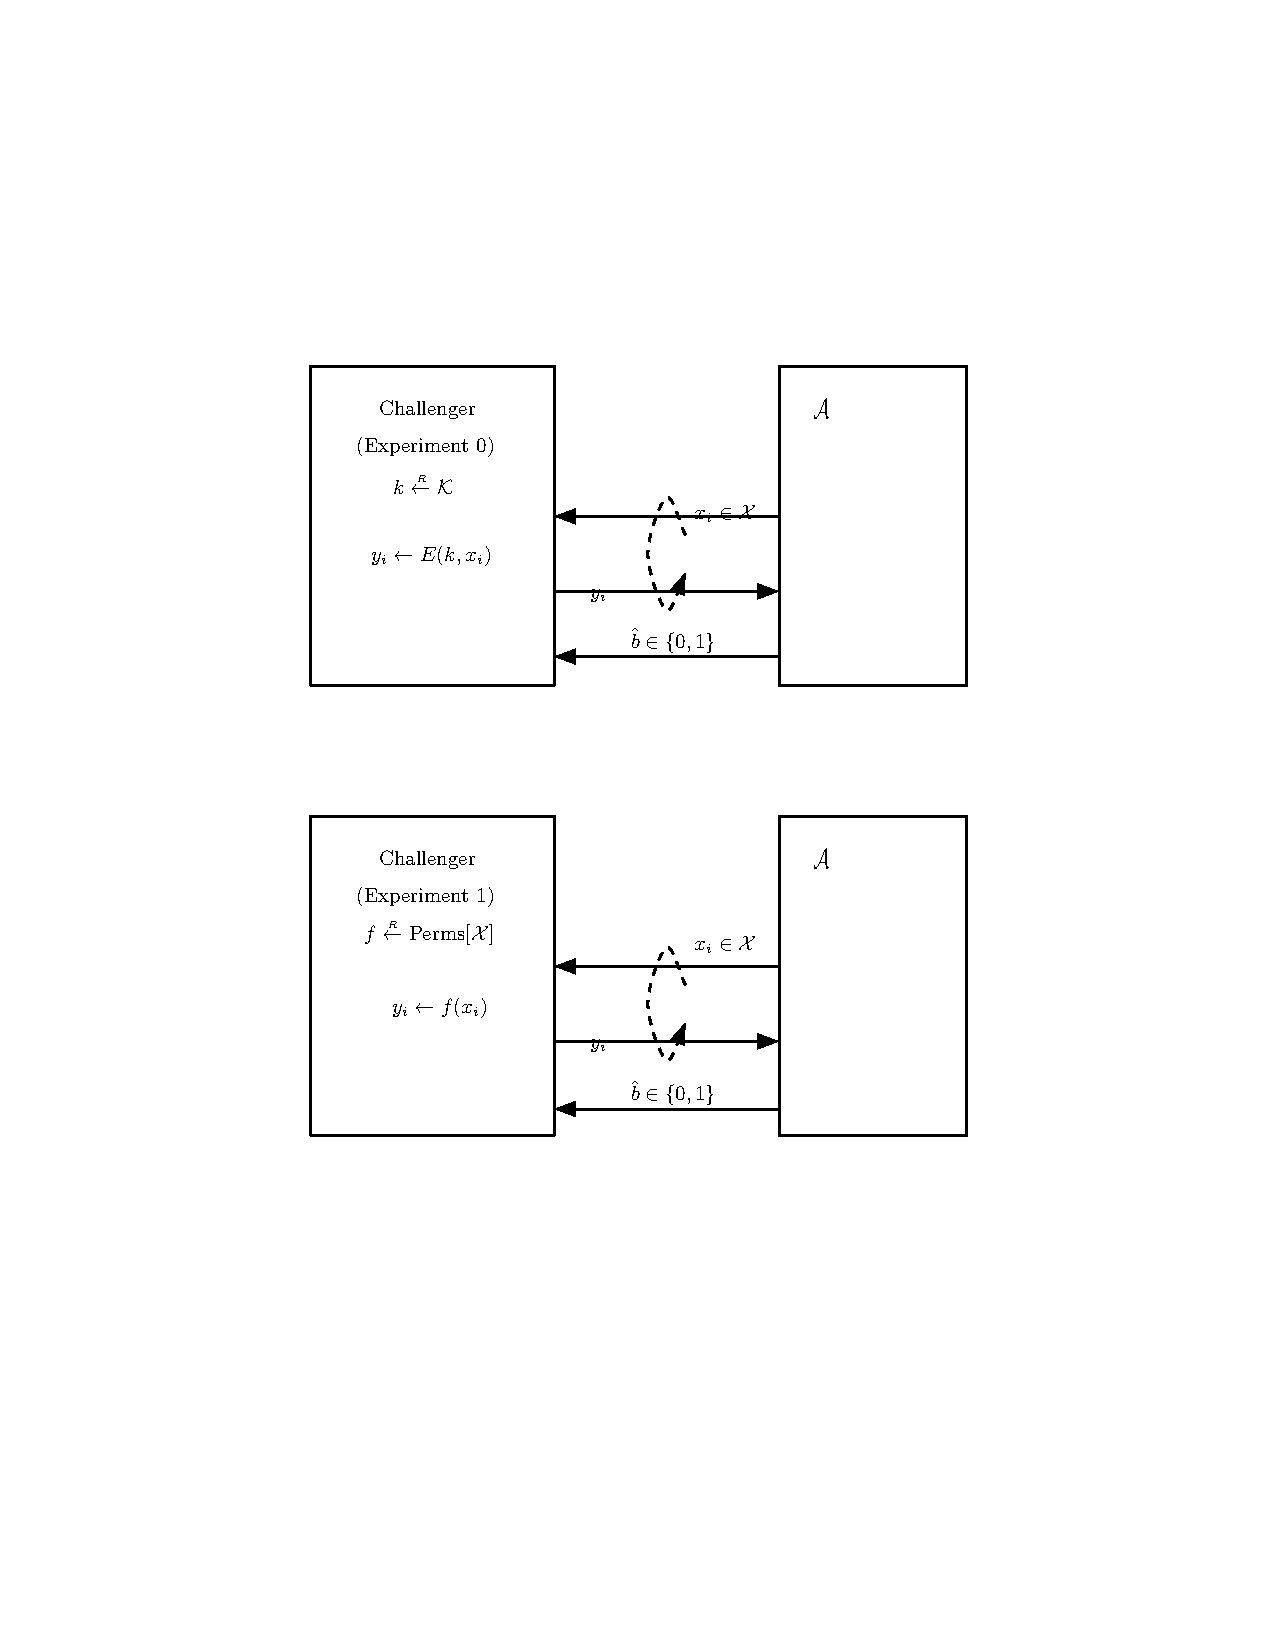
\includegraphics[scale=0.55]{crypto boneh book draft 115}\\
\captionsetup{labelsep=colon}
\caption{Adversary for a PRP}
\end{figure} 

\paragraph{}
 So let's look at a simple example. Suppose the set X contains only two points, zero and one. In this case, Perms[X] is really easy to define. Essentially, there are two points, and we're looking at, you know, 01. And we're asking, what is the set of all invertible functions on the set $\{0,1\}$. Well, there are only two such functions. One function is the identity function. And the other function is basically the function that does crossovers, namely this function here. These are the only two invertible functions in the set $\{0,1\}$. So really, Perms[X] only contains two functions, in this case. Now, let's look at the following PRP. The key space is going to be $\{0,1\}$, and of course, X is going to be $\{0,1\}$. And let's define the PRP as basically X XOR K.
 \qs{}{ So that's our PRP and my question to you is, is this a secure PRP. In other words, is this PRP indistinguishable from a random function on Perms[X]?}
 \sol Yes, because essentially, the sets of functions implemented in this PRP, is identical to the set of functions in Perms[X]. So a random choice of key here is identical to a random choice of function over here. And as a result, the two distributions, either pseudo-random or random, are identical. So clearly, an adversary can't distinguish the two distributions.
 \paragraph{} Now, we already said that we have a couple of examples of secure PRPs, Triple DES and AES. And I just wanted to mention that, if you want to make things very concrete, here's a concrete security assumptions about AES. Just to give an example, say that all algorithms had run in time $2^{80}$ have advantage against AES of utmost $2^{-40}$. This is, a reasonable assumption about AES, and I just wanted to state it for concreteness.
 \paragraph{} So let's look at another example. Consider again the PRP from the previous question. Namely X XOR K. Remember the set X was just one bit, namely the value zero and one. And this time, we're asking, is this PRP a secure PRF? In other words, is this PRP indistinguishable from a random function from X to X? Now, the set of random functions from X to X, Funs[XX] in this case, contains only four elements. There are the two invertible functions, the identity function, and the negation function, the function that sends zero to one, and one to zero. But there are two other functions. Namely, the function that sends everything to zero. And the function that sends everything to one. These are four functions inside Funs[XX], and the question is: 
 \qs{}{Is this PRP that we just looked at, is it also indistinguishable from a random choice from Funs[XX]?} 
 \sol \textbf{No} . The reason it's not a secure PRF is because there's a simple attack, namely the attacker supposed to distinguish whether he's interacting with this PRP or is he interacting with a random function from Funs[XX]. And the distinguisher is very simple. Basically we're going to query the function at both x=0 and x=1, and then if we get a collision, in other words, if $f_0 =  f_1$, then for sure we're not interacting with a PRP. In which case we can just output one. In other words we're interacting with a random function. In other words we say zero.
 \paragraph{} So let's look at the advantage of this distinguisher. Well when it's interacting with a PRP, it'll never output a one, because f of zero can never be equal to f of one. In other words, the probability of outputting one is zero. However, when we interact with a truly random function in Funs[XX], the probability that f of zero is equal to f of one is exactly $   \frac{1}{2} $. Cause half the functions satisfy f of zero's equal to f of one, and half the functions don't. So then, we'll output one with probability $   \frac{1}{2} $. So the advantage of this distinguisher is $   \frac{1}{2} $, which is non-negligible. And as a result, this PRP here is not a secure PRF. Now it turns out this only true because if set X is very small. And in fact there is an important lemma, called the PRF Switching Lemma, that says that a secure PRP, is in fact a secure PRF, whenever the set X is sufficiently large. And by sufficiently large, I mean say the output space of AES which is $2^{128}$. So by this lemma which will state more precisely in a second, AES if it's a secure PRP, it is also a secure PRF.
 \mlenma{}{Let E be a PRP over $(\mathcal{K},\mathcal{X})$. Then for any q-query adversary we have:
 \[ |Adv_{PRF}[\mathcal{A},E]-Adv_{PRP}[\mathcal{A},E]|\leq \frac{q^2}{2|\mathcal{X}|} 
 \]}
 \paragraph{} So this lemma basically says the following, if you give me a PRP over the set X Then for any adversary that queries the PRP, at at most Q points, so it makes at most Q queries into the challenge function. Then, the difference between its advantage in attacking the PRP when compared to a random function, is very close to its advantage in distinguishing the PRP from a random permutation. In fact the difference, is bounded by this quantity here, and since we said that X is very large, this quantity $\frac{q^2}{2|\mathcal{X}|}$ is negligible.  That's going to be our goal. So essentially, again, when X is large, say $2^{128}$ , Q say is going to be $2^{32}$. That's a billion queries that the adversary makes. Then, still the ratio is going to be negligible. In which case, we say that the adversary's advantage is distinguishing the PRP from a random function. It's pretty much the same as its advantage of distinguishing a PRP from a random permutation. So, again, it's basically, if E is already a secure PRP, then it's already a secure PRF.
 \paragraph{} So for AES, we believe, is a secure PRP. And therefore, AES, we can also use it as a secure PRF. And so, as a final note, I just want to mention that, really, from now on, you can kinda forget about the inner workings of AES and triple DES. We're simply going to assume that both are secure PRPs, and then we're going to see how to use them. But whenever I say PRP, or PRF, you should be thinking in your mind, basically, AES or Triple DES.
\subsection{Modes of Operation: One Time Key}

So as our first example lets look at a very simple way of using a block cipher for encryption. In particular we'll see how to use a block cipher with a one time key. So in this part we're just going to use the block cipher to encrypt using keys that are used one time. In other words, all the adversary gets to see is one ciphertext, and its goal is to break semantic security of that ciphertext. Now, in the next segment, we're going to turn into more, interesting applications of block ciphers and we're going to see how to encrypt using keys that are used many times to encrypt many messages.
\paragraph{}  I want to mention that there's like a classic mistake in using a block cipher. Unfortunately, there are some products that actually work this way, and they are badly broken, so I want to make sure that none of you guys actually make this mistake. So this mode of operation is called an electronic code book. And it works as follows: it's the first thing that comes to mind when you want to use a block cipher for encryption. What we do is we take our message, we break it into blocks, each block as big as the block's cipher block. So in the case of AES, we would be breaking our message into sixteen byte blocks. And then we encrypt each block separately. So this mode is often called electronic codebook. And, unfortunately, it's terribly insecure because you realize if two blocks are equal, for example here, these two blocks happen to be equal, then necessarily the resulting ciphertext is also going to be equal. So an attacker who looks at the ciphertext, even though he might not know what's actually written in these blocks, we'll know that these two blocks are equal. And as a result, he learned something about the plaintext that he shouldn't have learned.
\ex{}{
\paragraph{} And if this isn't clear enough for you abstractly, the best to explain this is using a picture. And so here's this guy here that, you know, has this really dark black hair. And when we encrypt. This image, this bitmap image using the electronic code book mode. You see that his hair, that contains lots of ones. Basically always gets encrypted the same way, so that his silhouette, actually, is completely visible, even in the encrypted data.
\begin{figure}[H]
\centering
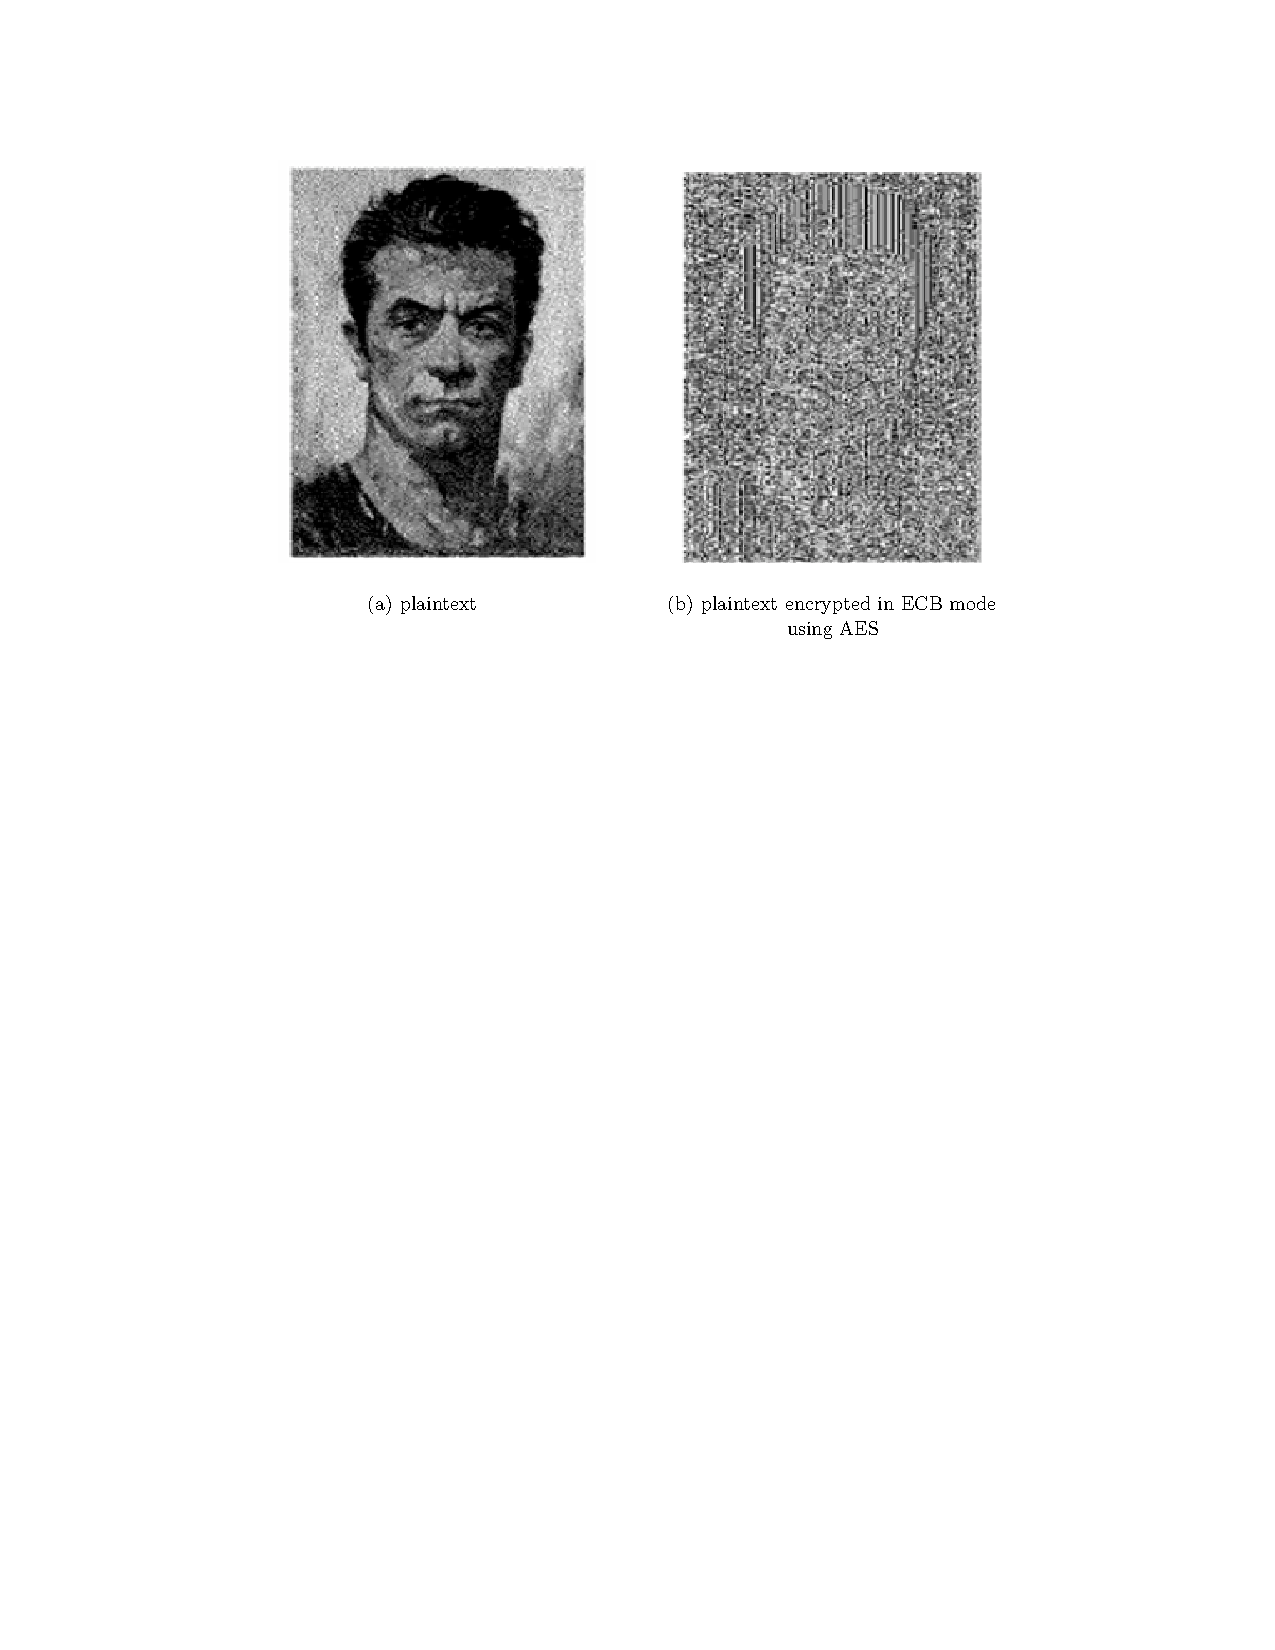
\includegraphics[scale=0.55]{crypto boneh book draft 120}\\
\captionsetup{labelsep=colon}
\caption{ECB example}
\end{figure} 

}
\paragraph{} So this is a nice example of how the electronic code book mode can actually leak information about the plaintext that could tell something to the attacker. So the question is, how to correctly use block ciphers to encrypt long messages. And so, I just want to briefly remind you of the notion we're trying to achieve, which is basically semantic security using a one-time key. So the adversary outputs two messages, $m_0$ and $m_1$, and then he gets either the encryption of $m_0$ or the encryption of $m_1$, these are two different experiments. And then our goal is to say that the adversary can't distinguish between these two experiments. So you can't distinguish the encryption of $m_0$ from the encryption of $m_1$. And the reason we call this security for a one-time key is that the key is only used to encrypt a single message. And as a result, the adversary will ever only see one ciphertext encrypted using this key.
\paragraph{} The first thing we want to show is that in fact the mode we just looked at, electronic code book, in fact, is not semantically secure. And this is true as long as you're encrypting more than one block.
\ex{Insecurity of ECB}{ Suppose we encrypt two blocks using a block cipher. Let me show you that in fact electronic code book will not be secure. So here's what we would do. So we're the adversary. So we would output two messages, $m_0$ and $m_1$, where, in one message, the blocks are distinct, and in the other message, the blocks are the same. The two blocks are equal to one another. Well, so what is the challenger going to do? The challenger's going to encrypt either $m_0$ or $m_1$. Either way we are going to get two blocks back. So the ciphertext actually contains two blocks. The first block is going to be an encryption of the word "Hello" and the second block is going to be either an encryption of the word "Hello" or the word "World". And if the two ciphertext blocks are the same then the adversary knows that he received an encryption of the message "Hello Hello" and as a difference he knows that he received encryption of the message "Hello World". So, he just follows a simple strategy here. And if you think about it for a second, you'll see what his advantage is. So, what is the advantage? Well, this adversary when he received an encryption of the message $m_1$ he will always output 0. and when he receives an encryption of the message $m_0$ it will always output 1. And because of that the advantage, basically, is 1, which means that the scheme is not secure, which again shows you the electronic code book is not semantically secure and should never ever be used to encrypt messages that are more than one block long.}
\paragraph{} So, what should we do? Well, so here's a simple example. What we could do is we could use what's called a deterministic counter mode. So in a deterministic counter mode, basically we build a stream cipher out of the block cipher. So suppose we have a PRF, F. So again you should think of AES when I say that. So AES is also a secure PRF. And what we'll do is, basically, we'll evaluate AES at the point zero, at the point one, at the point two, up to the point L. This will generate a pseudo random pad. And I will XOR that with all the message blocks and recover the ciphertext as a result.
\begin{figure}[H]
\centering
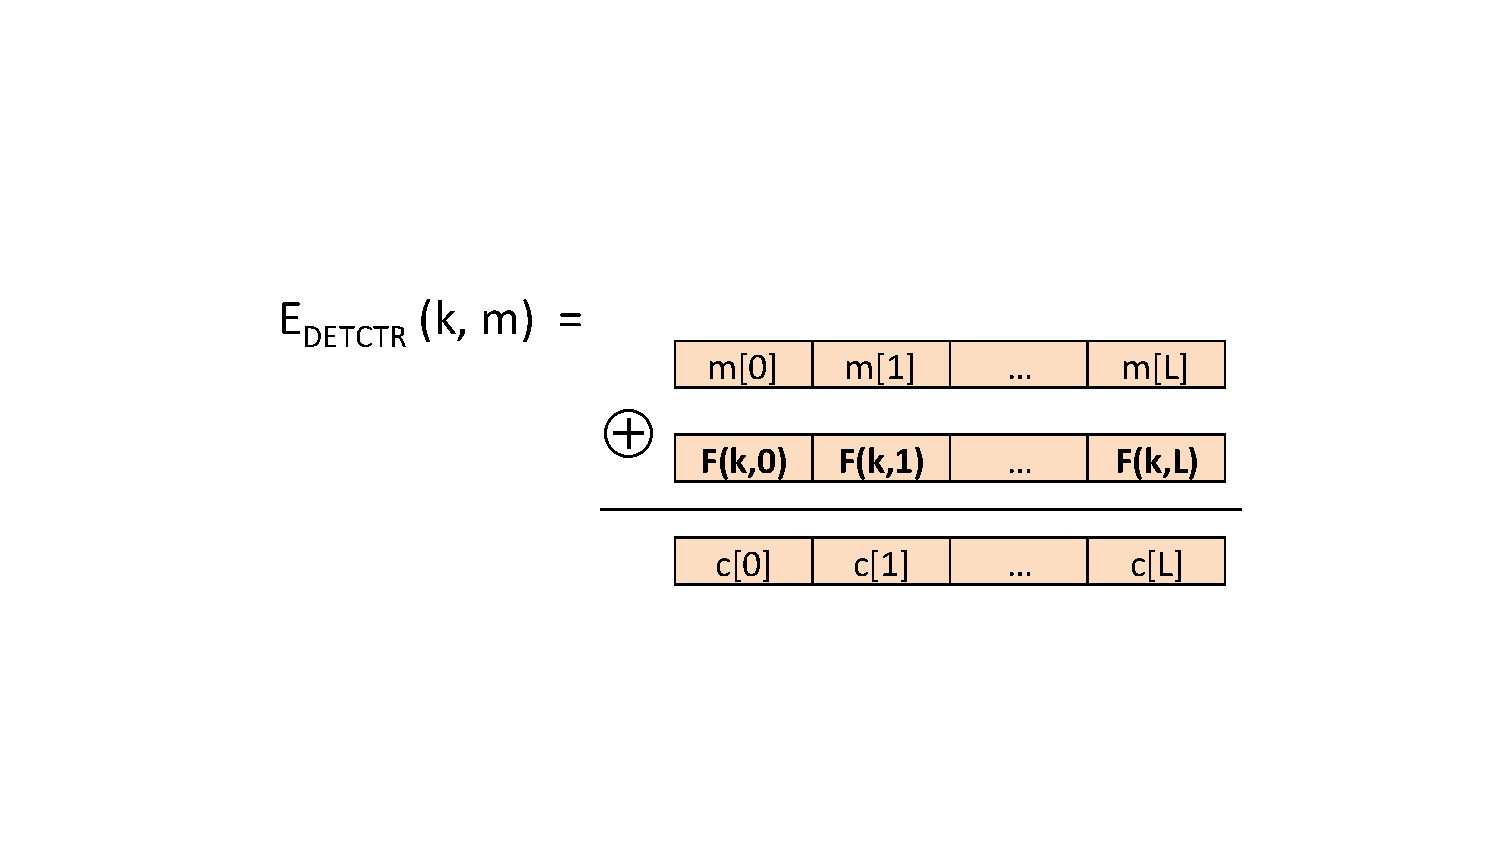
\includegraphics[scale=0.55]{04-using-block-v2-annotated 19}\\
\captionsetup{labelsep=colon}
\caption{Deterministic Counter Mode}
\end{figure}
\paragraph{} So really this is just a stream cipher that's built out of a PRF, like AES and triple DES, and it's a simple way to do encryption. I wanted to just very quickly show you the security theorem. In fact, we've already seen the security theorem when it applied to stream ciphers using pseudo-random generators, so I'm not going to repeat this again. I'll just remind you that essentially for every adversary A that's trying to attack deterministic counter mode, we prove that there's an adversary B that's trying to attack the PRF. And since this quantity is negligible, because the PRF is secure, we obtain that this quantity is negligible. And therefore, the adversary has negligible advantage in defeating deterministic counter mode. And the proof in pictures is a really simple proof. So I'll just show it to you one more time for completeness.
\thm{}{For any $L>0$ if F is a secure PRF over $(\mathcal{K},\mathcal{X},\mathcal{X})$ then $E_{DETCTR}$ is semantically secure over $(\mathcal{K},\mathcal{X}^L,\mathcal{X}^L)$. In particular, for every efficient adversary $\mathcal{A}$ attacking $E_{DETCTR}$ there exists an adversary $\mathcal{B}$ such that:
\[ Adv_{SS}[\mathcal{A}, E_{DETCTR}]=2 Adv_{PRF}[\mathcal{B}, F]
\]
}
\paragraph{} So basically, what we want to show is, when the adversary's given the encryption of the message $m_0$, here, this is the encryption of the message, $m_0$. $m_0$ XOR counter applied to the PRF, versus in giving the encryption of the message, $m_1$. We want to argue these two distributions are computationally indistinguishable. So the way we do that is basically we say, well the top distribution, if instead of a PRF, we use a truly random function, namely here f is a truly random function, then the adversary, because of the property of the PRF, the adversary cannot distinguish these two experiments, right. A PRF is indistinguishable from a truly random function, therefore when we replace the PRF on the left with a truly random function on the right, the adversary is going to behave the same. Basically you can't distinguish these two distributions. But now because f is a truly random function, the pad here is a truly one time pad, and therefore no adversary can distinguish an encryption of $m_0$ from an encryption of $m_1$ under the one time pad. So, again, these two distributions are the same. In fact, here there's an actual equality. These two distributions literally are the same distribution. And similarly again when we go back from a truly random function here to a PRF, because the PRF is secure, the adversary can't distinguish these two bottom distributions, the left from the right.
\begin{figure}[H]
\centering
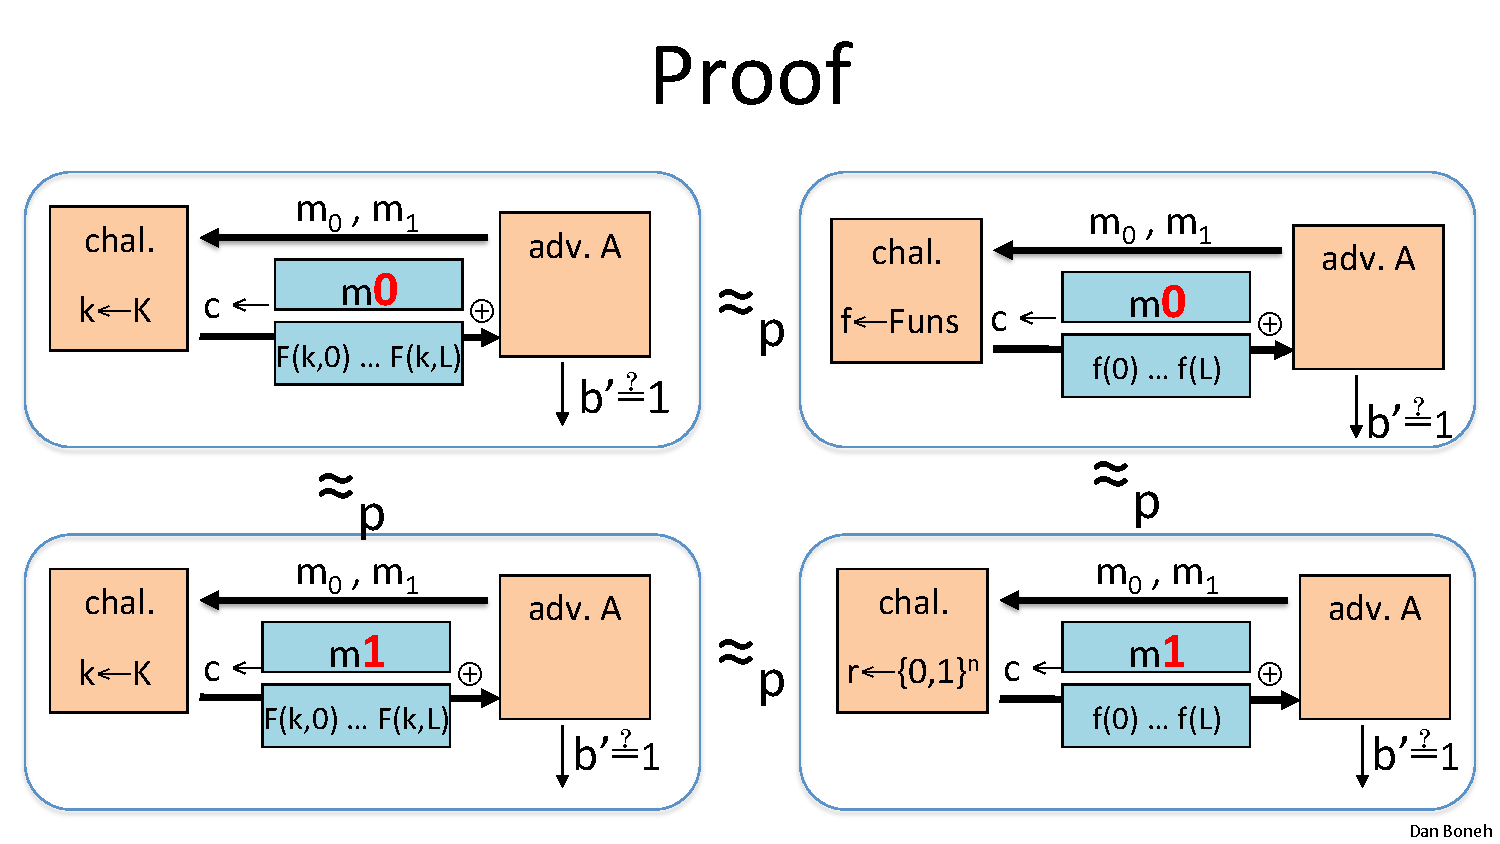
\includegraphics[scale=0.55]{04-using-block-v2-annotated 21}\\
\captionsetup{labelsep=colon}
\caption{Deterministic Counter Mode}
\end{figure}
\paragraph{} And so by following these three equalities, basically we have proven that the things we wanted to prove equal are actually computationally indistinguishable. So that's a very simply proof to show that deterministic counter mode is in fact secure and it's basically the same proof as we had when we proved that a stream cipher gives us semantic security.  So that completes this segment and in the next part we'll talk about modes that enable us to use a key to encrypt multiple messages.

\section{How to use Block Ciphers 2: Many-time key}
\subsection{Security for Many-Time Key (CPA security)}
\paragraph{}
In this part we will look at how to use block ciphers to encrypt multiple messages using the same key. This comes up in practice for example in file systems where the same key's used to encrypt multiple files. It comes up in networking protocols where the same key is used to encrypt multiple packets. So let's see how to do it. The first thing we need to do is to define what is mean for a cipher to be secure when the same key is used to encrypt multiple messages. When we use the key more than once the result of that is that the adversary gets to see many cipher text encrypted using the same key. As a result, when we define security, we're going to allow the adversary to mount what's called a chosen plain text attack. In other words, the adversary can obtain the encryption of arbitrary messages of his choice. So, for example, if the adversary's interacting with Alice. The adversary can ask Alice to encrypt arbitrary messages of the adversary's choosing. And Alice will go ahead and encrypt those messages and give the adversary the resulting cipher texts.
\paragraph{} You might wonder why would Alice ever do this. How could this possibly happen in real life? But it turns out this is actually very common in real life. And in fact, this modeling is quite a conservative modeling of real life. For example, the adversary might send Alice an email. When Alice receives the email, the writes it to her encrypted disk, thereby encrypting the adversary's email using her secret key. If later the adversary steals this disc, then he obtains the encryption of an email that he sent Alice under Alice's secret key. So that's an example of a chosen plain text attack, where the adversary provided Alice with a message and she encrypted that message using her own key. And then later the attacker was able to obtain the resulting cipher text. So that's the adversary's power. And then the adversary's goal is basically to break semantic security.
\paragraph{} So let's define this more precisely. As usual, we're going to define semantic security under a chosen plain text attack using two experiments, experiment zero and experiment one, that are modeled as a game between a challenger and an adversary. When the game begins, the challenger is going to choose a random key K. And now the adversary basically gets to query the challenger. So the adversary now begins by submitting a semantic security query, namely, he submits two messages, $m_0$ and $m_1$. I added another index, but let me ignore that extra index for a while. So the adversary submits two messages, $m_0$ and $m_1$, that happen to be of the same length. And then the adversary receives the encryption of one of those messages, either of $m_0$ or of $m_1$. In experiment zero, he receives the encryption of $m_0$. In experiment one, he receives the encryption of $m_1$.
\paragraph{} So far this would look familiar this looks exactly like a standard semantic security . However, plain text attack the adversary can now repeat this query again. So now you can issue a query with two other plain texts, again of the same length, and again you would receive the encryption of one of them. In experiment zero you would receive the encryption of $m_0$. In experiment one you would receive the encryption of $m_1$. And the attacker can continue issuing queries like this. In fact we'll say that he can issue up to Q queries of this type. And then, remember, every time he issues a pair of messages. That happen to be of the same length and every time he either gets the encryption of the left side or the right side again in experiment zero he will always get the encryption of the left message in experiment one he will always get the encryption of the left message. And, then adversary's goal is, basically, to figure out whether he's in experimental zero or in experiment one. In other words, whether he was constantly receiving the encryption of the left message or the encryption of the right message.
\dfn{CPA attack}{For a given cipher $E = (E,D)$, defined over $(\mathcal{K},\mathcal{M},\mathcal{C})$,
and for a given adversary $\mathcal{A}$, we define two experiments, Experiment 0 and Experiment 1. For
$b \in \{0, 1\}$, we define:\\
\textbf{Experiment} $b$
\begin{enumerate}
\item The challenger selects $k \xrightarrow{R} \mathcal{K}$.
\item The adversary submits a sequence of queries to the challenger. For $i=1,2,\ldots$ the ith query is a pair of messages $(m_{i0},m_{i1}) \in M$, of the same length. The challenger computes $c_i \xrightarrow{r} E(k,m_{ib})$, and sends $c_i$ to the adversary.
\item The adversary outputs a bit $\hat{b}\in \{0,1\}$.
\end{enumerate}
For $b \in \{0, 1\}$, let $W_b$ be the event that $\mathcal{A}$ outputs 1 in Experiment b.
We define $\mathcal{A}$'s semantic
security advantage with respect to E as
\[ Adv_{CPA}[\mathcal{A},\mathcal{E}] :=|Pr[W_0] - Pr[W_1]| \]
}
\paragraph{} In some sense, this is a standard semantic security game just iterated over many queries that the attacker can issue to adaptively one after the other. Now the chosen plain text attack is captured by the fact that if the attacker wants the encryption of a particular message m. What he could do is, for example, use query J for some J, where in this query J he'll set both the zero message and the one message to be the exactly same message M. In other words, both the left message and the right message are the same, and both are set to the message m. In this case, what he will receive, since both messages are the same, he knows that he's going to receive the encryption of this message m that he was interested in. So this is exactly what we meant by a chosen plaintext attack. Where the advisory can submit a message m and receive the encryption of that particular message m of his choice. So some of his queries might be of this chose plain text flavor where the message on the left is equal to the message on the right, but some of the queries might be standard semantic security queries where the two messages are distinct and that actually gives him information on whether he's in experiment zero or in experiment one. Now by now you should be used to this definition where we say that the system is semantically secure under a chosen plain text attack. If, for all efficient adversaries, they cannot distinguish experiment zero from experiment one. In other words, the probability that, at the end, the output, $b^\prime$, which we're going to denote by the output of experiment B. This output will be the same whether it was experiment zero or experiment one. So the attacker couldn't distinguish between always receiving encryptions of the left messages, versus always receiving encryptions of the right messages.
\dfn{CPA security}{A cipher E is called semantically secure against chosen
plaintext attack, or simply CPA secure, if for all efficient adversaries A, the value $Adv_{CPA}[\mathcal{A},\mathcal{E}]$
is negligible.}
\paragraph{} So in your mind, I'd like you to be thinking of an adversary that is able to mount a chosen plaintext attack, namely, be given the encryption of arbitrary messages of his choice, and his goal is to break semantic security for some other challenge cipher texts. And as I said in this  model of the real world the attacker is able to fool Alice into encrypting for him messages of his choice and then the attacker's goal is to somehow break some challenge ciphertext.
\clm{}{}{ I claim that all the ciphers that we've seen up until now, namely deterministic counter mode or the one time pad, are insecure under a chosen plain text attack. More generally, suppose we have an encryption scheme that always outputs the same cipher text for a particular message m. In other words, if I ask the encryption scheme to encrypt the message m once. And then I ask the encryption scheme to encrypt the message m again. If in both cases the encryption scheme outputs the same ciphertext, then that system cannot possibly be secure under a chosen plain text attack. And both deterministic counter mode and the one time pad were of that flavor. They always output the same cipher text, given the same message.}
\paragraph{} And so let's see why that cannot be chosen plain text secure. And the attack is fairly simple, what the attacker is going to do, is he's going to output the same message twice. This just says. That he really wants the encryption of $m_0$. So here the attacker is given $C_0$ which is the encryption of $m_0$. So this was his chosen plain text query where he actually received the encryption of the message $m_0$ of his choice. And now he's going to break semantic security. So what he does is he outputs two messages, $m_0$ and $m_1$ of the same length, and he's going to be given the encryption of MB. But  we said that the encryption system always outputs the same ciphertext when its encrypting the message, $m_0$. Therefore, if B=0, we know that C, this challenged ciphertext, is simply equal to $C_0$, because it's the encryption of $m_0$. However, if B=1. Then we know that this challenge cipher text is the encryption of $m_1$ which is something other than $C_0$ so all the attacker does is he just checks his $C = C_0$ the output's zero in other words he outputs one. So, in this case, the attacker is able to perfectly guess this bit B, so he knows exactly the experiment number given the encryption of $m_0$, or the encryption of $m_1$. And as a result, his advantage in winning this game is one. Meaning that the system cannot possibly be CPA secure. One is not a negligible number.
\paragraph{} So this shows that the deterministic encryption schemes cannot possibly be CPA-secure, but you might wonder well, what does this mean in practice? Well in practice this means again that every message is always encrypted to the same ciphertext. What this means is if you're encrypting files on disk, and you happen to be encrypting two files that happen to be the same, they will result in the same cipher text and then the attacker by looking at the encrypted disk, will learn that these two files actually contain the same content. The attacker might not learn what the content is, but he will learn that these two encrypted files are an encryption of the same content and he shouldn't be able to learn that. Similarly, if you send two encrypted packets on the network that happen to be the same, the attacker will not learn the content of those packets, but he will learn that those two packets actually contain the same information.
\ex{}{ Think for example of an encrypted voice conversation. Every time there's quiet on the line, the system will be sending encryptions of zero. But since encryption of zero are always mapped to the same cipher text. An attacker looking at the network will be able to identify exactly the points in the conversation where there's quiet because he will always see those exact same ciphertext every time. So these are examples where deterministic encryption cannot possibly be secure. And as I said formerly we say that  deterministic encryption can not be semantically secure under a chosen plain text attack.}
\paragraph{} So what do we do, well the lesson here is if the secret keys going to be used to encrypt multiple messages, it had better be the case that given the same plain text to encrypt twice. The encryption algorithm must produce different cipher texts. And so there are two ways to do that. The first method is what's called randomized encryption. Here, the encryption algorithm itself is going to choose some random string during the encryption process and it is going to encrypt the message m using that random string. So what this means is that a particular message, $m_0$ for example, isn't just going to be mapped to one cipher text but it's going to be mapped to a whole ball of cipher texts. Whereon every encryption, basically, we output one point in this ball.
\begin{figure}[H]
\centering
\includegraphics[scale=0.55]{04-using-block-v2-annotated 30}\\
\captionsetup{labelsep=colon}
\caption{Randomized encryption}
\end{figure}
\paragraph{}
 Every time we encrypt, the encryption algorithm chooses a random string, and that random string leads to one point in this ball. Of course, the decryption algorithm, when it takes any point in this ball, will always map the result to $m_0$. Similarly cipher text $m_1$ will be mapped to a ball, and every time we encrypt $m_1$, we basically output one point in this ball. And these balls have to be disjoint, so that the encryption algorithm, when it obtains a point in the ball corresponding to $m_1$, will always output the message $m_1$. In this way, since the encryption algorithm uses randomness, if we encrypt the same message twice, with high probability we'll get different cipher texts.
 \paragraph{} Unfortunately this means that the ciphertext necessarily has to be longer than the plain text because somehow the randomness that was used to generate the ciphertext is now encoded somehow in the cipher text. So the ciphertext takes more space. And roughly speaking, the cipher text size is going to be larger than the plain text by basically the number of random bits that were used during encryption. So if the plain texts are very big, if the plain texts are gigabytes long, the number of random bits is going to be on the order of 128. So maybe this extra space doesn't really matter. But if the plain texts are very short, maybe they themselves are 128 bits, then adding an extra 128 bits to every ciphertext is going to double the total ciphertext size. And that could be quite expensive. So as I say randomized encryption is a fine solution but in some cases it actually introduces quite a bit of costs.
\qs{}{ Imagine we have a pseudo random function that takes inputs in a certain space r which is going to be called a nonce space. And outputs, outputs in the message space. And, now, let's define the following randomized encryption scheme where we want to encrypt the message m with the encryption of whatever it's going to do is first it's going to generate a random r in this nonce space r. And then it's going to open a cipher text that consist of two components, the first component is going to be this value R and the second component is going to be an evaluation of the pseudo-random function at the point R XOR with the message M. And my question to you is, is this encryption system semantically secure under a chosen plain text attack?
\[ E(k,m)=[r \xleftarrow{R} R,\quad \text{ output } (r,F(k,r)\oplus m]\]
}
\sol \textbf{Yes}. But only if the nonce space r is large enough so that r never repeats with very, very high probability. And let's quickly argue why that's true. So first of all, because F is a secure pseudo-random function, we might as well replace it with a truly random function. In other words, this is indistinguishable from the case where we encrypt the message m, using the truly random function f, evaluated to point R, and then XOR with m. But since this little r never repeats every cipher text uses a different little r what this means is that the values of F(r) are random uniform independent strings every time. So every time we encrypt a message, we encrypt it essentially using a new uniform random one-time pad. And since XORing a uniform string with any string simply generates a new uniform string, the resulting cipher text is distributed as simply two random uniform strings. I'll call them r and $r^\prime$. And so both in experiment zero and in experiment one, all the attacker gets to see are truly uniform random strings r, r', and since in both experiments the attacker is seeing the same distribution, he cannot distinguish the two distributions. And so since security holds completely when we're using a truly random function it's also going to hold when we're using a pseudorandom function. So this is a nice example of how we use the fact that the pseudo random function behaves like a random function to argue security of this particular encryption scheme.
\paragraph{}  The other approach to building chosen plain text secure encryption schemes is what's called a \textbf{nonce} based encryption. Now, in a non-spaced encryption system, the encryption algorithm actually takes three inputs rather than two. As usual it takes the key and the message. But it also takes an additional input called a nonce. And similarly, the decryption algorithm also takes the nonce as input, and then produces the resulting decrypted plain text. This nonce value n is a public value. It does not need to be hidden from the adversary but the only requirement is that the pair (k,n) is only used to encrypt a single message. In other words, this pair (k,n) must change from message to message. 

\begin{figure}[H]
\centering
\includegraphics[scale=0.55]{04-using-block-v2-annotated 32}\\
\captionsetup{labelsep=colon}
\caption{Nonce-based encryption}
\end{figure}
\paragraph{} There are two ways to change it. One way to change it is by choosing a new random key for every message. And the other way is to keep using the same key all the time but then we must choose a new nonce for every message. And as mentioned, I want to emphasize again, this nonce need not be secret, and it need not be random. The only requirement is the nonce is unique. And in fact, we're going to use this term throughout the lecture. A nonce for us, means a unique value that doesn't repeat. It does not have to be random.
\paragraph{} So let's look at some examples of choosing a nonce, well the simplest option is simply to make the nonce a counter so for example the networking protocol you can imagine the nonce being a packet counter that's incremented every time a packet is sent by a sender or received by the receiver this means that the encrypter has to keep state from message to message mainly that he has to keep this counter around and increment it after every message is transmitted. Interestingly, if the decrypter actually has the same state then there is no need to include the nonce in the ciphertext since the nonce is implicit. 
\ex{}{
The https protocol is run over a reliable transport mechanism which means that packets sent by the sender are assumed to be received in order at a recipient. So if the sender sends packet \#5 and then packet \#6, the recipient will receive packet \#5 and then packet \#6 in that order. This means that if the sender maintains a packet counter, the recipient can also maintain a packet counter and two counters basically increment in sync. In this case there is no reason to include the nonce in the packets because the nonce is implicit between the two sides.
\paragraph{} However, in other protocols, for example, in IPsec, IPsec has a protocol designed to encrypt the IP layer. The IP layer does not guarantee in order delivery. And so the sender might send packet \#5 and then packet \#6, but those will be received in reverse order at the recipient. In this case it's still fine to use a packet counter as a nonce but now the nonce has to be included in the packet so that the recipient knows which nonce to use to decrypt the received packet.}
\paragraph{} So as mentioned, nonce based encryption is a very efficient way to achieve CPA security. In particular if the nonce is implicit, it doesn't even increase the ciphertext length. Of course another method to generate a unique nonce is simply to pick the nonce at random assuming the nonce space is sufficiently large so that with high probability the nonce will never repeat for the life of the key. Now in this case, nonce based encryption simply reduces to randomized encryption. However, the benefit here is that the sender does not need to maintain any state from message to message. So this is very useful for example if encryption happens to take place on multiple devices. For example, I might have both a laptop and a smart phone. They might both use the same key. But in this case if I require state full encryption, then my laptop and the smartphone would have to coordinate to make sure that they never reuse the same nonces. Whereas if both of them simply take nonces at random, they don't need to coordinate because it was very high probability they'll simply never choose the same nonce. Again assuming the nonce space is big enough. So there are some cases where stateless encryption is quite important, in particular where the same key is used by multiple machines.
\paragraph{} So I wanted to find, more precisely, what security means for nonce based encryption. And in particular, I want to emphasize that the system must remain secure when the nonce are chosen by the adversary. The reason it's important to allow the adversary to choose the nonces is because the adversary can choose which ciphertext it wants to attack. So imagine the nonce happens to be a counter and it so happens that when the counter hits the value fifteen, maybe at that point it's easy for the adversary to break semantic security. So the adversary will wait until the fifteenth packet is sent and only then he will ask to break semantic security. So when we talk about nonce based encryption, we generally allow the adversary to choose the nonce and the system should remain secure even under those settings. So let's define the CPA game in this case and it's actually very similar to the game before.

\dfn{Nonce-based CPA attack}{For a given cipher $E = (E,D)$, defined over $(\mathcal{K},\mathcal{M},\mathcal{C},\mathcal{N})$,
and for a given adversary $\mathcal{A}$, we define two experiments, Experiment 0 and Experiment 1. For
$b \in \{0, 1\}$, we define:\\
\textbf{Experiment} $b$
\begin{enumerate}
\item The challenger selects $k \xrightarrow{R} \mathcal{K}$.
\item The adversary submits a sequence of queries to the challenger. For $i=1,2,\ldots$ the ith query is a pair of messages $(m_{i0},m_{i1}) \in M$, of the same length and a nonce $n_i \in \mathcal{N}/\{n_1,\ldots n_{i-1}$. The challenger computes $c_i \xrightarrow{r} E(k,m_{ib},n_i)$, and sends $c_i$ to the adversary.
\item The adversary outputs a bit $\hat{b}\in \{0,1\}$.
\end{enumerate}
For $b \in \{0, 1\}$, let $W_b$ be the event that $\mathcal{A}$ outputs 1 in Experiment b.
We define $\mathcal{A}$'s semantic
security advantage with respect to E as
\[ Adv_{nCPA}[\mathcal{A},\mathcal{E}] :=|Pr[W_0] - Pr[W_1]| \]
}
\paragraph{} Basically the attacker gets to submit pairs of messages $m_i$, $m_{i0}$, and $m_1$. Obviously they both have to be of the same length. And he gets to supply the nonce. And in response, the adversary is given the encryption of either $m_{i0}$, or $m_1$. But using the nonce that the adversary chose. And of course, as usual, the adversary's goal is to tell whether he was given the encryption of the left plain text or the right plain text. And as before the adversary gets to iterate these queries and he can issue as, as many queries as he wants, we usually let q denote the number of queries that the adversary issues. Now the only restriction of course, which is crucial, is that although the adversary gets to choose the nonces, he's restricted to choosing distinct nonces. The reason we force him to choose distinct nonces is because that's the requirement in practice. Even if the adversary fools Alice into encrypting multiple messages for him, Alice will never use the same nonce again. As a result, the adversary will never see messages encrypted using the same nonce and therefore, even in the game, we require that all nonce be distinct.
\paragraph{} And then as usual we say that the system is a nonce based encryption system that's, semantically secure under a chosen plain text attack if the adversary cannot distinguish experiment zero where he's given encryptions of the left messages from experiment one where he's given encryptions of the right messages.
\dfn{nonce-based CPA security}{A cipher E is called semantically secure against chosen
plaintext attack, or simply CPA secure, if for all efficient adversaries A, the value $Adv_{nCPA}[\mathcal{A},\mathcal{E}]$
is negligible.} 
\qs{}{We have a secure PRF that takes inputs in the nonce space r and outputs strings in the message space m. Now when a new key is chosen, we're going to reset our counter r to be zero. And now we encrypt the particular message m, what we will do is we will increment our counter r, and then encrypt the message m using the pseudo random function applied to this value r. And as before, the ciphertext is going to contain two components, our current value of the counter and then the one time pad encryption of the message M. And so my question to you is whether this is a secure, non-spaced encryption system.
\[ E(k,m)=[r++,\quad \text{ output } (r,F(k,r)\oplus m]\]
}

\sol \textbf{Yes}, but only if the nuance space is large enough. So as we increment the counter r, it will never cycle back to zero so that the nuances will always, always be unique. We argue security the same way as before. Because the PRF is secure, we know that this encryption system is indistinguishable from using a truly random function. In other words, if we apply a truly random function to the counter and XOR the results with, the plain text m. But now since the nuance r never repeats, every time we compute this F of r, we get a truly random uniform and independent string so that we're actually encrypting every message using the one-time pad. And as a result, all the adversary gets to see in both experiments are basically just a pair of random strings. So both the experiment zero and experiment one the adversary get's to see exactly the same distribution, namely, the responses to all this chosen plain text queries are just pairs of strings that are just uniformly distributed and this is basically the same in experiment zero and experiment one and, therefore, the attacker cannot distinguish the two experiments. And since he cannot win the semantic security game with a truly random function he, also, cannot win the semantics security game with the secure PRF, and, therefore, the scheme is secure.
\paragraph{} So now we understand what it means for a symmetric system to be secure when the keys used to encrypt multiple messages the requirement is that it be secure under a chosen plan of attack. And we said that basically, the only way to be secure under a chosen plain text attack is either to use randomized encryption, or to use, use nonce spaced encryption where the nonce never repeats. And then in the next two segments, we're going to build two classic encryption systems that are secure when the key is used multiple times.
\subsection{Modes of Operation: Many Time Key (CBC)}
\paragraph{}
Now that we understand chosen plaintext security, let's build encryption schemes that are chosen plaintext secure. And the first such encryption scheme is going to be called cipher block chaining. So here is how cipher block chaining works. Cipher block chaining is a way of using a block cipher to get chosen plaintext security. In particular, we are going to look at a mode called cipher block chaining with a random IV. CBC stands for cipher block chaining. So suppose we have a block cipher, so EB is a block cipher.
\paragraph{} So now let's define \textbf{CBC} to be the following encryption scheme. So the encryption algorithm when it's asked to encrypt a message m, the first thing it's going to do is it's going to choose a random IV that's exactly one block of the block cipher. So IV is one cipher block. So in the case of AES the IV would be 16 bytes. And then we're going to run through the algorithm here, the IV basically that we chose is going to be XORed to the first plain text block. And then the result is going to be encrypted using the block cipher and output of the first block of the ciphertext. And now comes the chaining part where we actually use the first block of the ciphertext to kind of mask the second block of the plaintext. So we XOR the two together and the encryption of that becomes the second ciphertext block. And so on, and so on, and so forth. So this is cipher block chaining, you can see that each cipher block is chained and XORed into the next plaintext block, and the final ciphertext is going to be essentially the IV, the initial IV that we chose along with all the ciphertext blocks. I should say that IV stands for Initialization Vector. And we're going to be seeing that term used quite a bit, every time we need to pick something at random at the beginning of the encryption scheme typically we'll call that an IV for initialization vector.
\begin{figure}[H]
\centering
\includegraphics[scale=0.55]{04-using-block-v2-annotated 37}\\
\captionsetup{labelsep=colon}
\caption{CBC with random IV}
\end{figure}
\paragraph{} So you notice that the ciphertext is a little bit longer than the plain text because we had to include this IV in the ciphertexts which basically captures the randomness that was used during encryption. So the first question is how do we decrypt the results of CBC encryption, and so let me remind you again that if when we encrypt the first message block we XOR it with the IV, encrypt the result and that becomes the first ciphertext block.
\paragraph{}  How would you decrypt that? So given the first ciphertext block, how would you recover the original first plaintext block? So decryption is actually very similar to encryption, here I wrote down the decryption circuit, you can see basically it's almost the same thing except the XOR is on the bottom, instead of on the top, and again you realize that essentially we chopped off the IV as part of the decryption process and we only output the original message back, the IV is dropped by the decryption algorithm.
\begin{figure}[H]
\centering
\includegraphics[scale=0.55]{04-using-block-v2-annotated 38}\\
\captionsetup{labelsep=colon}
\caption{Decryption for CBC with random IV}
\end{figure}
\paragraph{} So the following theorem is going to show that in fact CBC mode encryption with a random IV is in fact semantically secure under a chosen plaintext attack, and so let's take that more precisely, basically if we start with a PRP, in other words, our block cipher E, that is defined over a space X, then we are going to to end up with a encryption algorithm ECBC that takes messages of length L and outputs ciphertexts of length L+1. And then suppose we have an adversary that makes q chosen plaintext queries. Then we can state the following security fact, that for every such adversary that's attacking ECBC, to exist an adversary that's attacking the PRP, the block cipher, with the following relation between the two algorithms, in other words, the advantage of algorithm A :  against the encryption scheme is less than the advantage of algorithm B : against the original PRP plus some noise term.
\thm{ECBC security}{If $\mathcal{E} = (E,D)$ is a secure block cipher defined over (K;X), and $N=|\mathcal{X}|$ is
super-poly, then for any poly-bounded $\ell\leq 1$, the cipher $\mathcal{E}^\prime$ described above is a CPA secure cipher.
In particular, for every CPA adversary $\mathcal{A}$ that attacks $\mathcal{E}^\prime$  which makes at most Q queries to its challenger, there exists PRP adversary B that attacks E  where B is an elementary wrapper around A, such that
\[
Adv_{CPA}[\mathcal{A}, \mathcal{E}^\prime] \leq \frac{2q^2\ell^2}{N}+ 2\times Adv_{PRP}[B; \mathcal{E}]:
\]
}
\paragraph{} Let me interpret this theorem for you as usual, so what this means is that essentially since E is a secure PRP this quantity here is negligible, and our goal is to say that adversary A's advantage is also negligible. However, here we are prevented from saying that because we got this extra error term. This is often called an error term and to argue that CBC is secure we have to make sure that the error term is also negligible. Because if both of these terms on the right are negligible, there sum is negligible and therefore the advantage of A against ECBC would also be negligible. So this says that in fact for ECBC to be secure it has better be the case that q squared L squared Is much, much smaller than the value X, so let me remind you what q and L are, so L is simply the length of the messages that we're encrypting. Okay, so L could be like say a 1000, which means that we are encrypting messages that are at most 1000 AES blocks. q is the number of ciphertexts that the adversary gets to see under the CPA attack, but in real life what q is, is basically the number of times that we have used the key K to encrypt messages, in other words if we use a particular AES key to encrypt 100 messages, Q would be 100. It is because the adversary would then see at most 100 messages encrypted under this key K.
\paragraph{}  See what this means in the real world. Suppose we want the adversary's advantage to be less than one over $2^{32}$. This means that the error term had better be less than one over $2^{32}$. So let's look at AES and see what this mean. For AES, AES of course uses 128 bit blocks, so X is going to be $2^{128}$, the size of X is going to be $2^{128}$, and if you plug this into the expression you see that basically the product q times L had better be less than $2^{48}$. This means that after we use a particular key to encrypt $2^{48}$ AES blocks we have to change the key. Okay, so essentially CBC stops being secure after the key is used to encrypt $2^{48}$ different AES blocks.
\paragraph{} So it's nice that the security theorem tells you exactly how long the key can be used and then how frequently, essentially, you have to replace the key. Now interestingly if you apply the same analogy to the Triple DES it actually has a much shorter block, maybe only 64 bits, you see the key has to be changed much more frequently, maybe after every 65 thousand DES blocks, essentially you need to generate a new key. So this is one of the reasons why AES has a larger block size so that in fact modes like CBC would be more secure and one can use the keys for a longer period of time, before having to replace it. What this means is having to replace $2^{16}$ blocks, each block of course is 8 bytes, so after you encrypt about half a megabyte of data you would have to change the DES key which is actually quite low. And you notice with AES you can encrypt quite a bit more data before you have to change the key.
\wc{}{ So I want to warn you about a very common mistake that people have made when using CBC with a random IV. That is that the minute that the attacker can predict the IV that you're going to be using for encrypting a particular message decipher this ECBC is no longer CPA secure. So when using CBC with a random IV like we've just shown It's crucial that the IV is not predictable.}
\paragraph{} But lets see an attack. So suppose it so happens that given a particular encryption in a message that attacker can actually predict that IV that will be used for the next message. Well let's show that in fact the resulting system is not CPA secure. So the first thing the adversary is going to do is, he is going to ask for the encryption of a one block message. In particular that one block is going to be zero. So what the adversary gets back is the encryption of one block, which namely is the encryption of the message namely zero, XOR the IV. Okay and of course the adversary also gets the IV. Okay so now the adversary by assumption can predict the IV that's going to be used for the next encryption. Let's say that IV is called, well IV. So next the adversary is going to issue his semantic security challenge and the message $m_0$ is going to be the predicted IV XOR IV1 which was used in the encryption of $c_1$. And the, the message of $m_1$ is just going to be some other message, it doesn't really matter what it is.
\begin{figure}[H]
\centering
\includegraphics[scale=0.55]{04-using-block-v2-annotated 41}\\
\captionsetup{labelsep=colon}
\caption{Attack on incorrectly implemented randomized CBC}
\end{figure}
\paragraph{} So now let's see what happens when the adversary receives the result of the semantic security challenge. Well, he is going to get the encryption of $m_0$ or $m_1$. So when the adversary receives the encryption of $m_0$, tell me what is the actual plain text that is encrypted in the ciphertext c? Well so the answer is that what is actually encrypted is the message which is IV XOR $IV_1$ XOR the IV that's used to encrypt that message which happens to be IV and this of course is $IV_1$. So when the adversary receives the encryption of $m_0$, he is actually receiving the block cipher encryption of $IV_1$. And lo and behold, you'll notice that he already has that value from his chosen plaintext query. And then, when he is receiving the encryption of message $m_1$, he just received a normal CBC encryption of the message $m_1$. So you realize that now he has a simple way of breaking the scheme, namely what he'll do is he'll say, he's going to ask, "Is the second block of the ciphertext c equal to the value that I received in my CPA query?" If so I'll say that I received the encryption of $m_0$, otherwise I'll say that I received the encryption of $m_1$. So really his test is $c_1$ he refers to the second block of c and $c_{11}$ refers to the second block of $c_1$, if the two are equal he says zero, otherwise he says one. So the advantage of this adversary is going to be 1 and as a result, he completely breaks CPA security of this CBC encryption.
\begin{note} So the lesson here is, if the IV is predictable then, in fact, there is no CPA security and unfortunately, this is actually a very common mistake in practice. In particular even in SSL protocol and in TLS 1.1, it turns out that IV for record number I is in fact the last ciphertext block of record I-1. That means that exactly given the encryption of record I-1, the adversary knows exactly what IV is going to be used as record number I. Very recently, just last summer, this was actually converted into a pretty devastating attack on SSL. We'll describe that attack once we talk about SSL in more detail, but for now I wanted to make sure you understand than when you use CBC encryption, its absolutely crucial that the IV be random.
\end{note}
\paragraph{} Now I going to show you the nonce based version of CBC encryption So in this mode the IV is replaced by non random but unique nonce for example the numbers 1,2,3,4,5, could all be used as a nonce, and now, the appeal of this mode is that if the recipient actually knows what the nonce is supposed to be then there's no reason to include the nonce in the ciphertext, in which case, the ciphertext is exactly the same length as the plaintext, unlike CBC with the random IV, where we had to expand the ciphertext to include the IV, here, if the nonce is already known to the recipient, there's no reason to include it in the ciphertext, and the ciphertext is exactly the same length as the plaintext.
\begin{figure}[H]
\centering
\includegraphics[scale=0.55]{04-using-block-v2-annotated 42}\\
\captionsetup{labelsep=colon}
\caption{Nonce-based CBC}
\end{figure}
\paragraph{} So it's perfectly fine to use a non-random but unique nonce. However, it's absolutely crucial to know that, if you do this, there's one more step that you have to do before you use the nonce in the CBC chain. In particular, in this mode now we're going to be using two independent keys, k and $k_1$. The key k is, as before, going to be used to encrypt the individual message blocks, However, this key $k_1$ is going to be used to encrypt the non-random but unique nonce, so that the output is going to be a random IV, which is then used in the CBC chain. So this extra step here, encrypting the nonce with the key $k_1$, is absolutely crucial. Without it, CBC mode encryption would not be secure. However it if is going to be a counter you need to do one more step. Before actually encryption CBC and in particular you have to actually encrypt the notes to obtain the IV that will actually be used for encryption.
\paragraph{} The nonce on CBC is similar to a random IV, the difference is that the nonce is first encrypted and the results is that the IV is used in the CBC encryption Now the beauty of this mode is that the nonce doesn't necessarily have to be included in the cipher text. It only needs to be in there if its unknowns are the decrypter but it if the decrypter happens to already know the value of the counter by some other means then in fact the cipher text is only as big as the plain text. There's no extra value transmitted in the cipher text. And again, I warn that when you're using non spaced encryption, it's absolutely crucial that the key common nonce spare is only used for one message so for every message, either the Nonce has changed or the key has changed. Okay, so here emphasize the fact that you need to do this extra encryption step before actually using the nonce.
\paragraph{} This is very common mistake that actually forgotten in practice and for example in TLS, this was not done and as a result there was a significant attack against CBC encryption in TLS. Remember the reason that this is so important to know is that in fact many crypto APIs are set up to almost deliberately mislead the user to using CBC incorrectly. So let's look to see how CBC implemented inside of open SSL.
\paragraph{}
\begin{figure}[H]
\centering
\includegraphics[scale=0.45]{04-using-block-v2-annotated 43}\\
\captionsetup{labelsep=colon}
\caption{OpenSSL API}
\end{figure}
\paragraph{} So here are the arguments of the function. Basically this is the plain text, this is the place where the cipher text will get written to. This is the length of the plain text. This is a, a Yes key Finally there is an argument here that says whether you are encrypting or decrypting. And the most important parameter that I wanted to point out here is the actual IV and unfortunately, the user is asked to supply this IV and the function uses the IV directly in the CBC encryption mechanism. It doesn't encrypt the IV before using it and as a result, if you ever call this function using a non random IV, the resulting encryption system won't be CPA secure.
\paragraph{} It's very important to know that when calling functions like this. CBC encryption or open SSL either supply a truly random IV or if you want the IV to be a counter than you have to encrypt a counter using AAS before you actually call a CBC encrypt and you have to that yourself. So again, it's very important that the programmer knows that it needs to be done otherwise the CBC encryption is insecure. One last technicality about CBC is what to do when the message is not a multiple of the block cipher block length? That is what do we do if the last message block is shorter than the block length of AES, for example? So the last message block is less than 16 bytes. And the answer is if we add a pad to the last block so it becomes as long as sixteen bytes, as long as the AES block size. And this pad, of course, if going to be removed during encryption.
\begin{figure}[H]
\centering
\includegraphics[scale=0.45]{04-using-block-v2-annotated 44}\\
\captionsetup{labelsep=colon}
\caption{CBC with padding}
\end{figure}
\paragraph{} So here is a typical path, this is the path that is used in TLS. Basically a pad with n bytes then essentially what you do is you write the number n, n times. So for example if you pad with five bytes, you pad with the string 555555. So five bytes where each byte is the value five. And the key thing about this pad is basically when the decrypter receives the message, what he does is he looks at the last byte of the last block. So suppose that value is five, then he simply removes the last five bytes of the message. Now the question is what do we do if in fact the message is a multiple of sixteen bytes so in fact no pad is needed? If we don't pad at all, well that's a problem because the decrypter is going to look at the very last byte of the last block which is not part of the actual message and he's going to remove that many bytes from the plain text. So that actually would be a problem. So the solution is, if in fact there is no pad that's needed, nevertheless we still have to add a dummy block. And since we add the dummy block this would be a block that's basically contains sixteen bytes each one containing the number 16. So we add essentially 16 dummy blocks. The decrypter, that when he's decrypting, he looks at the last byte of the last block, he sees that the value is sixteen, therefore he removes the entire block. And whatever's left is the actual plain text.
\paragraph{} So it's a bit unfortunate that in fact if you're encrypting short messages with CBC and the messages happen to be, say, 32 bytes, so they are a multiple of sixteen bytes, then you have to add one more block and make all these ciphertexts be 48 bytes just to accommodate the CBC padding. I should mention there's a variant of CBC called CBC with ciphertext stealing that actually avoids this problem, but I'm not going to describe that here. So that's the end of our discussion of CBC and in the next part we'll see how to use counter modes to encrypt multiple messages using a single key.

\subsection{Modes of Operation: Many Time Key (CTR)}
\paragraph{}
In this part we're going to look at another method to achieve chosen plain text security that's actually superior to CBC. And this method is called randomized counter mode. Unlike CBC. Randomized counter mode uses a secure PRF. It doesn't need a block cipher. It's enough for counter mode to just use a PRF because we're never going to be inverting this function F. So we're going to let F be the secure PRF and it acts on n byte blocks. Again if we use AES, N will be 128. And the way the encryption algorithm works in counter mode is it starts off by choosing a random IV, that's 128 bytes random IV in the case of AES, and the essentially we start counting. From this random IV, so you notice the first encryption is of IV then IV+1 up to IV+L. So we generate this random pad. We XOR the result with the message, and that gives us the ciphertext. 
\begin{figure}[H]
\centering
\includegraphics[scale=0.45]{04-using-block-v2-annotated 47}\\
\captionsetup{labelsep=colon}
\caption{Randomized Counter Mode}
\end{figure}
\paragraph{}
Notice that the IV here is included along with the ciphertext. So that, in fact, the cipher text is a little longer than the original plain text. And the point, of course, is that, encryption algorithm chooses a new IV for every message. And so even if I encrypt the same message twice, I'm going to get different resulting cipher texts.
\paragraph{} One thing to notice that this mode is completely parallelizable, unlike CBC. CBC was sequential. In other words, you couldn't encrypt block \#5 until you've encrypted blocks \#1 to \#4, so hardware companies who might have multiple AES engines working in parallel cannot actually use those AES engines when using CBC because CBCs inherently sequential. So even though you might have two or three of four AES engines, you could only use one of them when doing CBC encryption. With counter mode, everything is completely parallelizable. If you have three AES engines encryption basically will work three times as fast. So that's the beauty of counter mode. And counter mode also has a corresponding nonce based counter mode. Where the IV is not truly random, but rather, is just a nonce which could be a counter. And the way you would implement nonce based counter mode, is you would take the 128 bits block that used in AES. And then you would split it in two. You would use the left 64 bits as the nonce, so the counter say would count from zero to $2^{64}$.That will be the nonce part of it. And then once you specify the nonce, the lower order, 64 bits, would be doing the counting inside of the counter modes encryption.
\begin{figure}[H]
\centering
\includegraphics[scale=0.45]{04-using-block-v2-annotated 48}\\
\captionsetup{labelsep=colon}
\caption{Nonce-based Counter Mode}
\end{figure}
 So nonce goes on the left, and the counter mode encryption counter goes on the right. And it's perfectly fine if this nonce is unpredictable. The only restriction is that you encrypt at most $2^{64}$ blocks using one particular nonce. The danger is that you don't want this counter to reset to zero so that, then, you will have two blocks. Say, this guy, this guy, and this guy that are encrypted using the same one time pad. Namely this one and this one. So lets quickly state the security theorem for a randomized counter mode. By now you should be used to these kind of theorems. Basically we are given a secure PRF. What we end up with is an encryption scheme. We'll call it $E_{CTR}$, which is semantically secure under a chosen plain text attack. It encrypts messages that are L blocks long, and produces cipher text that are L+1 blocks long because the IV has to be included in the ciphertext.
\thm{Randomized Counter Mode security}{If F is a secure PRF and $N=|\mathcal{X}|$ is
super-poly, then for any poly-bounded $\ell\leq 1$, the cipher $\mathcal{E}^\prime$ described above is a CPA secure cipher.
In particular, for every CPA adversary $\mathcal{A}$ that attacks $\mathcal{E}^\prime$  which makes at most q queries to its challenger, there exists PRF adversary B that attacks where B is an elementary wrapper around A, such that
\[
Adv_{CPA}[\mathcal{A}, \mathcal{E}^\prime] \leq \frac{2q^2\ell}{N}+ 2\times Adv_{PRF}[B, \mathcal{E}]:
\]
}
 
 \paragraph{} This is for randomized counter mode. And the error bounds are stated over here. It's basically the same bounds as in the case of CBC encryption. As usual, we argue that this term is negligible because the PRF F is secure and we would like to deduce from that, that this term is negligible so that $E_{CTR}$ is secure. Unfortunately we have this error term here and so we have to make sure this error term is negligible. And for that we have to make sure q squared L is less than the size of a block. And remember, q is the number of messages encrypted under a particular key. And L is the maximum length of those messages. Now interestingly in the case of CBC we have q squared L squared. Has to be less than x. Which is actually worse than we have for counter modes. In other words, counter modes can actually be used for more blocks than CBC could.
 \paragraph{} Lets see a quick example of that. So here is, again, the error term for counter-node, and remember q is again the number of messages encrypted with a key, and L is the length of those messages. And as before, just as in the case of CBC, suppose we want the adversary's advantage to be at most, one over $2^{32}$. That basically requires that this q-squared, L over X be less than 1 over $2^{64}$. So for AES what happens is, if you plug in the values X is $2^{128}$, 128 bit blocks. So q times square root of L should be less than $2^{48}$. This is basically the bound you get from plugging in $2^{128}$ into this bound here. And as a result, you can see if you're encrypting messages that are each, $2^{32}$ blocks. Then after $2^{32}$ such messages you have to replace your secret key otherwise randomized counter mode is no longer CPA secure. So this means we could encrypt a total of $2^{64}$ AES blocks using a single secret key. Remember, for CBC the corresponding value was $2^{48}$ blocks so in fact because counter mode has a better security parameterization in fact we can use the same key to encrypt more blocks with counter mode than we could with CBC.
 \paragraph{} So I wanted to do a quick comparison of counter mode and CBC and argue that in every single aspect, counter mode is superior to CBC. And that's actually why most modern encryption schemes actually are starting to migrate to counter mode, and abandoned CBC. Even though CBC is still quite widely used. So let's look at the comparison.
\begin{table}[H]
\centering
 \begin{tabular}{||c c c||} 
 \hline
  & CBC & CTR  \\ [0.5ex] 
 \hline\hline
 uses & PRP & PRF \\ 
 parallel processing & no & yes \\
 security & $\frac{q^2L^2}{|X|}$ & $\frac{q^2L}{|X|}$ \\
 dummy padding block & yes & no \\ 
 one-byte messages &16x expansion & no expansion \\[1ex] 
 \hline
 \end{tabular}
\end{table} 
  First of all, recall that CBC actually had to use a block cipher because if you look at the decryption circuit, the decryption circuit actually ran the block cipher in reverse. It was actually using the decryption capabilities of the block cipher. Whereas in counter mode, we only use a PRF. We never ever, ever use the decryption capabilities of the block cipher. We only use it in the forward direction, only encrypt with it. Because of this, counter mode is actually more general and you can use primitives like Salsa, for example, Salsa20, if you remember, as a PRF. But is not a PRP. So counter mode can Salsa but CBC cannot. And in essence, counter mode is more general than CBC. Counter mode, as we said, is actually parallel, whereas CBC is a very sequential process. We said that counter mode is more secure. The security bounds, the error terms are better for counter mode than they are for CBC. And as a result, you can use a key to encrypt more blocks in counter mode than you could with CBC. The other issue is, remember in CBC we talked about the dummy padding block. If you had a message that's a multiple of the block length. In CBC we said that we had to add a dummy block whereas in counter mode this wasn't necessary. Although, I did want to mention that there is a variation of CBC called CBC with cipher text tiling, that actually avoids the dummy block issue. So for standardized CBC, we actually need a dummy block. But in fact there is a modification to CBC that doesn't need a dummy block. Just like counter mode.
  \paragraph{} Finally, suppose you're encrypting just a stream of one byte messages, and using nonce encryption with an implicit nonce. So, the nonce is not included in the ciphertext. In this case. Every single one byte message would have to be expanded into a sixteen byte block and then encrypted, and the result would be a sixteen byte block. So if you have, like, a stream of 100 one byte messages, each one separately would have to become a sixteen byte block. And you'll end up. With a stream of 116 byte ciphertexts. So you get a 16x expansion on the length of the cipher text, compared to the length of the plain text. In counter mode, of course, this is not a problem. You would just encrypt each one byte message by XORing with the first bytes of the stream that's generated in the counter mode. So every cipher text would just be one byte, just like the corresponding plain text. And so no expansion at all, using counter mode. So you see that essentially, every single aspect counter mode dominates CBC. And that's why it's actually the recommended mode to be using today.
  \paragraph{} This concludes our discussion of chosen plaintext security. I wanted to just quickly summarize and remind you that we're going to be using these PRP and PRF abstractions of block ciphers. This is actually the correct way of thinking of block ciphers and so we'll always think of them as either pseudorandom permutations or pseudorandom functions. And then I wanted to remind you again that, so far, we saw two notions of security. Both only provide security against eavesdropping. They don't provide security against tampering with the ciphertext. One was used when the key is only used to encrypt a single message. The other one was used when the key was used to encrypt multiple messages.
  \begin{figure}[H]
\centering
\includegraphics[scale=0.45]{04-using-block-v2-annotated 52}\\
\captionsetup{labelsep=colon}
\caption{Summary}
\end{figure}
  \paragraph{} And as mentioned, because neither one is designed to defend against tampering, neither one provides data integrity. And we're going to see this as a real problem. And as a result, in fact, I'm going to say in the next chapter that these modes actually should never, ever be used. You should only be using these modes in addition to an integrity mechanism, which is our next topic. So, so far we've seen basically for using a, the key once, you can use stream ciphers or you can use deterministic counter mode. If you're going to use the key many times you could use randomize CBC or randomize counter mode and we're going to talk about how to provide integrity and confidentiality. Once we cover the topic of integrity, which is our next module.

\chapter{Message Integrity}

\section{Definitions}
\subsection{Message Authentication Codes}
\paragraph{} In this module, we're going to stop talking about encryption, and instead discuss message integrity. Next, we will come back to encryption, and show how to provide both encryption and integrity. 
\paragraph*{}
So as mentioned, our goal here is to provide integrity without any confidentiality. There are actually in fact many cases in the real world where this comes up. For example, you can think of operating system files on your disk. Say if you're using Windows, all the Windows operating system files on disk are not confidential, they're public and known to the world, but it is quite important to make sure that they're not modified by a virus or some malware. That's an example where you want to provide integrity but you don't care about confidentiality.
\paragraph*{}
 Another example is banner ads on web pages. The provider of the ads doesn't care at all if someone copies them and shows them to other people. So there's no confidentiality issue at all. But they do care about modifying those ads. So, for example, they do want to prevent people from changing the ads into different types of ads. So that's another example where integrity matters but confidentiality is not important at all.
\paragraph*{}
 So how do we provide message integrity? The basic mechanism is what's called a MAC, a message authentication code, MAC. And the way we do it is as follows. So here we have our friends, Alice and Bob. They have a shared key, $k$, which is not known to the attacker, but known to both of them. And there's a public message $m$ that Alice wants to send to Bob, such that an attacker along the way cannot modify this message on its way to Bob. The way Alice does it, is by using what's called a MAC signing algorithm S, where the MAC signing algorithm takes as input the key and the message, and produces a very short tag. The tag could be like 90 bits or 100 bits, or so on. Even though the message is gigabytes long, the tag is actually very, very short. 
 \paragraph*{} 
 Next, she appends the tag to the message and sends the combination of the two to Bob. Bob receives the message and the tag, and then he runs what's called a MAC verification algorithm on this tag. The MAC verification algorithm takes as input to the key, the message, and the tag and it says yes or no, depending on whether the message is valid or whether it's been tampered with. 
 
\begin{figure}[H]
\centering
\includegraphics[scale=0.65]{fig1}\\
\captionsetup{labelsep=colon}
\caption{Overview of the problem setting}
\end{figure}
 \paragraph*{} So more precisely, what is a MAC? Well, we said the MAC basically consists of two algorithms, a signing algorithm and a verification algorithm. As usual, they're defined over a key space, a message space, and a tag space. And as we said, it's a pair of algorithms. So the signing algorithm will output a tag in the tag space, and the verification algorithm, basically given the key, the messages and the tag, will output yes or no. And I want to remind you as usual there are these consistency requirements, such that for every K in the key space and for every message in the message space, it so happens that if I sign a message using a particular key, and then I verify the tag using the same key, I shall get yes in response. So this is the standard consistency requirement which is the analog of the one that we saw for encryption. 
\dfn{MAC System}{A MAC system $\mathcal I = (S, V )$ is a pair of efficient algorithms, S and V , where S
is called a signing algorithm and V is called a verification algorithm. Algorithm S is used to
generate tags and algorithm V is used to verify tags.
\begin{itemize}
\item S is a probabilistic algorithm that is invoked as $t\xleftarrow R S(k,m)$, where k is a key, m is a message,
and the output t is called a tag.
\item V is a deterministic algorithm that is invoked as $r\leftarrow V(k, m, t)$, where k is a key, m is a
message, t is a tag, and the output r is either accept or reject.
\item We require that tags generated by S are always accepted by V ; that is, the MAC must satisfy
the following correctness property: for all keys k and all messages m,
\begin{equation}
Pr[V(k,m,S(k,m))=accept]=1
\end{equation}
\end{itemize}
}
 
 
\paragraph*{} Now, one thing I'd like to point out is that integrity really does require a shared key between Alice and Bob. And, in fact, there's a common mistake that people make, where they try to provide integrity without actually a shared key.
\begin{note}
Integrity against malicious (non-random) errors requires a shared key between the two parties. 
\end{note}

\paragraph*{} 
\ex{}{So here's an example. Consider CRC. CRC stands for cyclic redundancy check. This is a classic checksum algorithm that's designed to detect random errors in messages. So imagine, instead of using a key to generate the tag, Alice basically uses a CRC algorithm which is keyless. Doesn't take any key, to generate a tag. And then she appends this tag to the message, she sends it over to Bob, Bob will basically verify that the CRC is still correct. In other words, Bob will still verify the tag is equal to CRC(m). And if so the verification algorithm will say yes, and otherwise the verification algorithm will say no. So the problem with this is this is very easy for an attacker to defeat. In other words, an attacker can very easily modify the message and route, and fool Bob into thinking that the new message is a valid one.
\paragraph{} The way the attacker will do it is he'll cancel the message in the tag. He'll simply block them. And then he'll produce his own message, $m^\prime$, and compute his own CRC on this message $m^\prime$, and then send the concatenation of the two over to Bob. Bob will run the verification algorithm, verification will work properly because in fact the right-hand side is in fact a valid CRC for the left-hand side. And as a result, Bob would think that this message came from Alice but in fact its been completely modified by the attacker and had nothing to do with the original message that Alice sent.\\
\paragraph{}  So the problem is, because CRC doesn't have a key, there's no difference between Alice and the attacker. And as a result, Bob doesn't know where the message came from. Once we introduce a key, now Alice can do something that the attacker can't do. And as a result, she might be able to compute a tag that the attacker can't modify. So the point to remember is that CRC is designed to detect random errors, not malicious errors. And here our goal is to make sure that even a malicious attacker cannot modify messages en route.
}
  \paragraph*{} So next we want to define what it means for a MAC system to be secure. So as usual, we define security in terms of the attacker's power. What can the attacker do? And the attackers goal. What is he trying to do? So in the case of MACs, the attacker's power is what's called a chosen message attack. In other words, the attacker can give Alice arbitrary messages of his choice, $m_1, \ldots , m_q$, and Alice will compute the tag for him on those messages, and give him those tags.\\
   So again, you might wonder, why would Alice ever do that? Why would Alice ever compute the tag on a message that the attacker gave her? So just like in the case of chosen plaintext attack, it's very common in the real world, that the attacker can give Alice a message. Alice will compute the tag on that message, and then the attacker will obtain the resulting tag. For example, the attacker might send Alice an email. Alice might want to save the email to disk in a way that will prevent someone from tampering with the disk. So she'll compute a tag on the message, and save the message and the tag to disk. Later on, the attacker might steal Alice's disk. And now he's recovered Alice's tag on the message that he sends to Alice. 
   \paragraph*{} So this is an example of a chosen message attack in the real world, where the attacker actually obtained a tag on a message that he gave Alice. Okay, so that's what the attacker can do, basically, this chosen message attack. And what is his goal? Well, his goal is to do something called an \textbf{existential forgery}. What he's trying to do is to produce some, some new valid message tag pair that is different from one of the pairs that were given to him during the chosen message attack. And if he can do that, then we say that the system is insecure, and if he can't, then we'll say the system is secure.
   
   \dfn{Existential Forgery}{Existential forgery is a type of cryptographic attack where an attacker can produce at least one valid but unintended message or signature without necessarily having control over the exact content of the message or the actual private key used for signing. In other words, the attacker can create a message or signature that is not meaningful in any practical context but is still valid according to the cryptographic scheme.\\
   	\\
   	Existential forgery attacks are a concern in various cryptographic scenarios, including digital signatures and encryption.}
   
   
   \paragraph*{} So I want to emphasize this existential forgery means that the attacker cannot produce a new message/tag pair $(m,t)$, even for a message that's completely gibberish. And again, you might wonder, well, why do we care if the attacker computes a tag on a message that's gibberish? That's not of any value to the attacker. But we want to build MACs that are secure under any usage settings. And there are, in fact cases where, for example, you might want to compute an integrity tag on a random secret key. In which case, even if the attacker is able to compute a tag on a completely random message, he might be able to fool a user into using the wrong secret key. And as a result we want to make sure that if the MAC is secure, the attacker can't produce a valid tag for any message whether it's gibberish or sensical.\\
    Another property that's implied by the security definition is if the attacker is given some message tag pair he shouldn't be able to produce a new tag for the same message. In other words, even though there might be another tag $t^\prime$ for the same message m, the attacker given m and t shouldn't be able to find this new $t^\prime$ and again you might wonder well why do we care the attacker already has a tag on message $m$. Why does it matter if he can produce another tag for the message $m$ he already has one tag. But as we'll see, there are actually applications where it's really important that the attacker not to be able to produce a new tag for a previously signed message. In particular, this will come up when we combine encryption and integrity. So that we are going to demand that given one tag in the message it's impossible to find another tag for the same message. \paragraph*{} Okay, so now that we understand the intuition of what we are trying to achieve, let's define it as usual using a more precise game.
    Here we have two algorithms S and V, and we have an adversary A, and the game proceeds as follows. The challenger as usual just chooses a random key for the MAC and the adversary basically does his chosen message attack. So he submits an $m_1$ to the challenger and receives the tag on that message $m_1$. Then he submits an $m_2$ to the challenger and receives a tag on that $m_2$. And so on and so forth, until, you know, he submits Q messages to the adversary and receives Q tags on all those messages. \\
    Then the adversary goes ahead and tries to do an existential forgery. Namely, he outputs a message tag pair, a new message tag pair. We say that he wins the game, in other words, b=1 means that he wins the game if, first of all, the message tag pair that he outputs is a valid message tag pair, so the verification algorithm says yes. And second of all, it's a fresh message tag pair. In other words, it's not one of the message tag pairs that we gave him before. In other words we say that the attacker lost the game, namely, b=0. 
\paragraph*{}    And as usual we say, we define the advantage of an adversary as the probability that the challenger outputs one in this game. We say that the MAC system is secure if for all efficient adversaries the advantage is negligible. Okay, in other words, no efficient adversary can win this game with non negligible probability. That's our definition of secure MACs, and our goal is to build secure MACs like this.
\dfn{Attack on MAC}{
For a given MAC system $\mathcal I = (S, V )$, defined over
$(K,M, T)$, and a given adversary A, the attack game runs as follows:
\begin{itemize}
\item The challenger picks a random k uniformly.
\item A queries the challenger several times. For $i =1,\ldots q$  the ith signing query is
a message $m_i \in M$. Given $m_i$, the challenger computes a tag $t_i  \xleftarrow R S(k,m_i)$, and
then gives $t_i$ to A.
\item Eventually A outputs a candidate forgery pair $(m, t)\in (M,T)$ that is not among
the signed pairs, that is,
\begin{equation*}
(m,t)\notin \{(m_1,t_1),\ldots ,(m_q,t_q)\}
\end{equation*}
\end{itemize}

Note that in the case of a deterministic signing algorithm, $t_i  \xleftarrow R S(k,m_i)$ becomes $t_i = S(k,m_i)$
}

\dfn{Secure MAC}{A MAC is considered secure if $MAC_{adv}=Pr[V(k,m,t)=accept]$ is negligible}

\begin{figure}[H]
\centering
\includegraphics[scale=0.85]{crypto boneh book draft 234}\\
\captionsetup{labelsep=colon}
\caption{Figure descibing the attack}
\end{figure}

 Before we do that, I want to ask you two questions.
\qs{}  {Suppose we have a MAC. And it so happens that the attacker can find two message, $m_0$ and $m_1$, that happen to have the same tag for about half of the keys. In other words, if you choose a key at random with probability $\frac{1}{2}$, the tag of the message $m_0$ will be the same as the tag of the message $m_1$. And my question to you is can this be a secure MAC. So I want to emphasize the attacker doesn't know what the tag on $m_0$ and $m_1$ is. All he knows is that the two messages happen to have the same tag with probability one half. Is this a secure MAC?} 
\sol
The answer is no, this is not a secure MAC and the reason is because of the chosen message attack. Essentially the attacker can ask for the tag on the message $m_0$, then he will receive ($m_0$, t) from the challenger and in fact t would be a valid tag for message $m_0$ and then what he would output as his existential forgery is $(m_1, t)$ and you notice that $m_1$, T is different from $m_0$, T, so this is a valid existential forgery. And as a result, the attacker wins the game with advantage one-half. So we conclude that this MAC is not secure. 
\qs{}{Suppose we have a MAC that happens to always output a five bit tag. In other words, the tag space for this Mac happens to be $\{0,1\}^{5}$ . So for every key and for every message, the signing algorithm will just output a five bit tag. And the question is, can this MAC be secure?}
\sol Of course the answer is no, because the attacker can simply guess the tag. So what he would do is he wouldn't ask any chosen message attacks. All he would do, is he would output an existential forgery as follows. He would just choose a random tag. So choose a random tag t at random in $\{0,1\}^5$, and then he would just output his existential forgery as say, the message zero and the tag t. And now with probability of $(\frac{1}{2})^5$, this tag will be a valid tag for the message zero. And so the adversary's advantage is $(\frac{1}{32})$, which is non-negligible. So this basically says that tags can't be too short. They have to have some length to them. And in fact, the typical tag length would be, say 64 bits. or 96 bits, or 128 bits. Here let's for example use the tags that are 96 bits long. If you try to guess the tag for a message when the tag is 96 bits the probability of guessing it correctly is $(\frac{1}{2})^{96}$. So the adversary's advantage would just be $(\frac{1}{2})^{96}$ which is negligible.
\paragraph*{}


 So now that we understand what MACs are, I want to show you a simple application. In particular, let's see how MACs can be used to protect system files on disk. So imagine that when you install an operating system, say, when you install Windows on your machine. One of the things that, Windows does, is it asks the user for a password, and then derives a key K from this password. And then for every file that it writes to disk, in this case, the files would be $F_1,F_2,\ldots F_n$, what the operating system would do is it would compute a tag for that file, and then store the tag along with the file. So here it concatenates the tag, to each one of the files. And then it erases the key K. So it no longer stores the key K on disc, or on memory, or anywhere.
 \begin{figure}[H]
\centering
\includegraphics[scale=0.55]{05-integrity-v2-annotated 9}\\
\captionsetup{labelsep=colon}
\caption{Encrypting files}
\end{figure}
 Okay, so now later imagine that the machine gets infected with a virus and the virus tries to modify some of the system files. The question is whether the user can detect which files were modified. So here's one way to do it. Basically, the user would reboot the machine into some clean OS. Say you reboot from a USB disk or something. And then, once the machine boots from this clean OS, the user would supply his password to this clean running operating system. And then this new clean running operating system would go ahead and check the MAC for each one of the system files. Now, the fact that the MAC is secure, means that the poor virus couldn't actually create a new file, let's call it $F^\prime$, with a valid tag. So it couldn't actually create an $F^\prime$, $t^\prime$. Because, if it could, then that would be an existential forgery on this MAC. And because, well, the MAC is existentially unforgeable. The virus couldn't create any $F^\prime$, no matter what the $F^\prime$ is. And consequently, because of the security of the MAC, the user will detect all the files that were modified by the virus.
 \paragraph*{} Now, there's one caveat to that. One thing that the virus can do. Is actually swap two files. So, for example, he can swap this file, file $F_1$, with the file $F_2$ here, just literally swap them. So when the system, or when the user, tries to run file $F_1$, instead they'll be running file $F_2$. And of course that could cause all sorts of damage. And so the way to defend against that is essentially by placing the file name inside of the MACed area, so in fact we're computing an integrity check on the file name as well as on the contents of the file. And as a result, if the virus tries to swap two files, the system will say hey, the file that's located in position $F_1$ doesn't have the right name and therefore it will detect that the virus that did the swap even though the MAC actually verifies. So it is important to remember that MACs can help you defend against file tampering. Or data tampering in general. But they won't help you defend against swapping of authenticated data, and that has to be done by some other means. That concludes our introduction to MACs, and in the next segment, we'll go ahead and construct our first examples of secure MACs.
 
\subsection{MAC Based on PRFs}
Now that we know what MACs are, let's go ahead and build our first secure MACs. First I want to remind you that a MAC is a pair of algorithms. The first is a signing algorithm that's given a message and a key will generate a corresponding tag And the second is verification algorithms are given a key message and a tag while outputs zero or one depending on whether the tag is valid or not. And we said that a MAC is secure if it is existentially unforgeable under a chosen message attack. In other words, the attackers allow to mount a chosen message attack where he can submit arbitrary messages of his choice and obtain the corresponding tags for those messages, and then despite the ability to generate arbitrary tags The attacker cannot create a new message-tag pair that was not given to him during the chosen message attack.
\paragraph{} Okay so we've already seen this definition in the last section and now the question is how do we build secure MACs? So the first example I want to give you is basically showing that any secure PRF directly gives us a secure MAC as well. So let's see how we do it. So suppose we have a pseudo random function so the pseudo random function takes and inputs X and outputs in Y. And let's define the following MAC. So the way we sign a message 'M' is basically by simply evaluating the function at the point 'M' So the tag for the message M is simply the value of the function at the point M and then the way we verify a message to that pair is by recomputing the value of the function at the message M and checking whether that is equal to the tag given to us. We say yes if so and we reject otherwise. So here you have in pictures basically that when Alice wants to send a message to Bob she computes a tag by the value of PRF and then she appends this tag to the message, Bob receives the corresponding tab pair, he recomputes the value of the function and tests whether the given tag is actually equal to the value of the function at the point M.
\dfn{Deterministic MAC derived from a psuedo-random function F}{
\begin{equation}
\begin{split}
S(k,m):= F(k,m)\\
V(k,m)=\begin{cases}
\mathrm{accept} & \text{if}\,t= F(k,m)\\
\mathrm{reject} & \text{otherwise}
\end{cases}
\end{split}
\end{equation}
}

\paragraph{}
\qs{}{Suppose that we have a pseudo-random function that happens to output only ten bits. Okay, so this is a fine pseudo-random function and it just so happens that for any message 'M' it only outputs ten bits value. My question to you is if we use this function 'F' to construct a MAC, is that going to be a secure MAC?}
\sol So the answer is no, this MAC is insecure. In particular because the tags are too short. So consider the following simple adversary. What the adversary will do is simply choose an arbitrary message M and just guess the value of the MAC for that particular message. Now, because the tag is only ten bits long, the adversary has a chance of one in $2^{10}$ in guessing the MAC correctly. In other words, the advantage of the guessing adversary, one distinctly guesses a random tag for a given message. That adversary is going to have an advantage against the mac that's basically $(\frac{1}{2})^{10}$ which is one over a thousand twenty four and that's definitely non negligible. So the adversary basically will successfully forge the mac on a given message with probability one on a thousand which is insecure. 
\paragraph{} However it turns out this is the only example that where things can go wrong, only when the output of the function is small can things go wrong. If the output of the PRF is large Then we get a secure MAC out of this function. And let's state the security theorem here. 

\thm{}{If $F:K\times X\rightarrow Y$ is a secure PRF and $\frac{1}{|Y|}$ is negligible then $I_F$ is a secure MAC. In particular, for every adversary A attacking $I_F$ there exists an efficient adversary $B$ attacking $F$ such that:
\[
\text{Adv}_{\text{MAC}}(A,I_F)\leq \text{Adv}_{\text{PRF}}(B,F)+\frac{1}{|Y|}
\]
}
\paragraph{} So suppose we have a function 'F' that takes messages in 'X' and outputs tags in 'Y', then the MAC that's derived from this PRF in fact is a secure MAC. In particular, if you look at the security theorem here, you'll see very clearly the error bounds, in other words since the PRF is secure we know that this quantity here is negligible. And so if we want this quantity to be negligible,  that no adversary can defeat the MAC '$I_F$', that implies that we want this quantity to be negligible, in other words we want the output space to be large. And so for example, taking a PRF that outputs eighty bits is perfectly fine. That will generate an eighty bit MAC and therefore the advantage of any adversary will be at most $(\frac{1}{2})^{80}$.
\paragraph{}

 So now the proof of this theorem is really simple, so lets just go ahead and do it. So in fact lets start by saying that suppose instead of a PRF we have a truly random function from the message space to the tag space so this is just a random function from X to Y that's chosen at random from the set of all such functions. Now lets see if that function can give us a secure mac. 
 
\begin{figure}[H]
\centering
\includegraphics[scale=0.55]{05-integrity-v2-annotated 16}\\
%\captionsetup{labelsep=colon}
\caption{}
\end{figure} 
 
 
\paragraph{} So what the adversary says is, 'I want a tag on the message $m_1$'. What he gets back is the tag which just happens to be the function evaluated at the point $m_1$. Notice there is no key here because f is just a truly random function from X to Y. And then the adversary gets to choose a message from $m_2$ and he obtains the tag from $m_2$, he choose $m_3$, $m_4$ up to $m_q$ and he obtains all the corresponding tags. Now his goal is to produce a message tag pair and we say that he wins, remember that this is an existential forgery, in other words, first of all $t$ has to be equal to $f(m)$ This means that '$t$' is a valid tag for the message '$m$'. And second of all, the message '$m$' has to be new. So the message '$m$' had better not be one of $m_1,...,m_q$. But let's just think about this for a minute, what does this mean? So the adversary got to see the value of a truly random function at the points 
$m_1,...,m_q$ and now he suppose to predict the value of this function as some new point, $m$. However, for a truly random function, the value of the function at the point $m$ is independent of its value at the points $m_1,...,m_q$.
\paragraph{} So the best the adversary can do at predicting the value of the function at the point $m$ is just guess the value, because he has no information about $f(m)$. And as a result his advantage if he guesses the value of the function at the point $m$ he'll guess it right with exact probability of $\frac{1}{|Y|}$. And then the tag that he produced will be correct with exact probability of $\frac{1}{|Y|}$. Okay, again he had no information about the value of the $f(m)$ and so the best he could do is guess. And if he guesses, he'll get it right with probability $\frac{1}{|Y|}$. And now of course, because the $f$ is a pseudo random function The adversary is going to behave the same whether we give him the truly random function or the pseudo random function. The adversary can't tell the difference and as a result even if we use a pseudo random function, the adversary is going to have advantages at most $\frac{1}{|Y|}$ in winning the game. 
\paragraph{} Okay, so you can see exactly the security theorem, let's go back there for just a second. Essentially this is basically why we got an error term of $\frac{1}{|Y|}$ because of the guessing attack and that's the only way that the attacker can win the game.
\paragraph{} So now that we know that any secure PRF is also a secure MAC, we already know that we have our first example MAC. In particular, we know that AES, or at least we believe that AES is a secure PRF, therefore, AES since it takes sixteen byte inputs, right the message space for AES is 128 bits, which is sixteen bytes. Therefore the AES cipher essentially gives us a MAC that can match messages that are exactly sixteen bytes. Okay, so that's our first example of a MAC. 
\paragraph{} But now the question is if we have a PRF for small inputs like AES that only acts on sixteen bytes, can we build a MAC for big messages that can act on gigabytes of data? Sometimes I call this the McDonald's problem. Basically given a small MAC and we build a big MAC out of it. In other words, given a MAC for small messages and we build a MAC for large messages. So we're going to look at two constructions for doing so. The first example is called a CBC-MAC that again takes PRF for small messages as input and produces a PRF for very large messages. As outputs. The second one we'll see is HMAC which does the same thing again takes a PRF for small inputs and generates a PRF for very large inputs.
\paragraph{} Now the two are used in very different contexts. CBC-MAC is actually very commonly used in the banking industry. For example, there's a system called the Automatic Clearing House, ACH, which banks use to clear checks with one another and that system, CBC-MAC, is used to ensure integrity of the checks as they're transferred from bank to bank. On the Internet, protocols like SSL and IPsec and SSH, those all use HMAC for integrity. Two different MACs and were going to discuss them in the next couple of segments. And as I said were also going to start from a PRF for small messages and produce PRF for messages that are gigabytes long and in particular they can both be substantiated with AES as the underlying cipher.
\paragraph{} So the last comment I want to make about these PRF based MACs is that in fact their output can be truncated. So suppose we have a PRF that outputs N bit outputs. So again for AES this would be a PRF that outputs 128 bits as outputs. 
\mlenma{}{
Its an easy lemma to show that in fact if you have an N bit PRF if you truncated, in other words if you only output first key bits The result is also a secure PRF and the intuition here is if the big PRF outputs N bits of randomness for any inputs that you give to the PRF then certainly chopping it off and truncating it to T bits is still going to look random.
\paragraph{} The attacker now gets less information so his job of distinguishing the outputs from random just became harder. In other words, if the N bit PRF is secure, then the T less than N bit PRF, the truncated PRF, would also be secure.}
\paragraph{} So this is an easy lemma and since any secure PRF also gives us a secure MAC, what this means is if you give me a MAC that's based on a PRF and what I can do is I can truncate it to W bits, however, because of the error term in the MAC based PRF theorem we know that truncating to W bits will only be secure as long as one over two to the W is negligible. So if you truncate the PRF to only three bits, the resulting MAC is not going to be secure. However, if you truncate it to say 80 bits or maybe even 64 bits, then the resulting MAC is still going to be a secure MAC.
\paragraph{} Okay, so the thing to remember here is that even though we use AES to construct larger PRFs and the output of these PRFs is going to be 128 bits, it doesn't mean that the MAC itself has to produce 128 bit tags We can always truncate the outputs to 90 bits or 80 bits, and as a result, we would get still secure MACs but now the output tag is going to be more reasonable size and doesn't have to be the full 128 bits. In the next segment we're going to look at how the CBC-MAC works.

\section{Constructions}
\subsection{CBC-MAC and NMAC}
In this section, we're going to construct two classic MACS, the CBC-MAC and the NMAC. Recall in the last section, we said that if you give me a secure PRF, then that secure PRF can actually be used to construct a secure MAC, simply by defining the signature on the message m as the value of the function at the point m. 
\paragraph{} The only caveat was that the output of the PRF F had to be large. For example, it could be 80 bits or 128 bits, and that would generate a secure MAC Now we also said that because AES is a secure PRF, essentially AES already gives us a secure MAC, except that it can only process sixteen byte messages. And the question now is, given a PRF for short messages like AES for sixteen byte messages, can we construct a PRF for long messages that are potentially gigabytes long? And this is shorthand for what's coming. I'm going to denote by X, the set $\{0,1\}^N$ where N is the block size for the underlying PRF.
\paragraph{} So since we're always going to be thinking of AES as the underlying PRF, you can think of N as essentially 128 bits. So the first construction is called the encrypted CBC-MAC, or ECBC for short. Encrypted CBC-MAC. So ECBC uses a PRF that takes messages in the set X $\{0,1\}^N$ and outputs messages in the same set X. And what we're going to be building is a PRF that basically takes pairs of keys. It takes very long messages, in fact arbitrarily long messages, and I'll explain this in just a second and it outputs also tags in $\{0,1\}^N$. So that's our goal.
\begin{figure}[H]
\centering
\includegraphics[scale=0.55]{05-integrity-v2-annotated 22}\\
\captionsetup{labelsep=colon}
\caption{ECBC}
\end{figure} 

\paragraph{} Now what is this X to the less than or equal to L? The point here is that in fact CBC-MAC can take very long messages up to L blocks. L could be a million or a billion. But it could also take variable length messages as inputs. In other words, X less than or equal to L means that we allow the input to be messages that contain an arbitrary number of blocks between one and L. So each CBC can process messages that are one block long, two blocks long, ten blocks long, 100 blocks long. It's perfectly fine to give it variable size inputs. But just to keep the discussion simple, we up our bounds the maximum length by capital L.
\paragraph{} So let's see how ECBC works. Well, we start by taking our message and breaking it into blocks, each block is as long as a block of the underlying function f, and then essentially we run through the CBC chain except that we don't output intermediate values. So you notice we basically encrypt the first block and then feed the results into the XOR with the second block and then feed that into f again, and we do that again and again and again and finally we get a value out here. Which is called the CBC outputs of this long chain. And then, I would like to point your attention to the fact that we do one more encryption step. And this step is actually done using an independent key, $K_1$. That's different and chosen independently of the key K, and finally the output gives us the tag.
\paragraph{} So in this case the tag would be N bits long, but we also mentioned in the previous section that it's fine to truncate the tag to less than N bits long as long as one over $2^{n}$ is negligible. So now you can see that FECBC takes a pair of keys as inputs, it can process variable length messages and it produces an output in the set X. So you might be wondering what this last encryption step is for. And I'll tell you that the function that's defined without this last encryption step is called the \textbf{raw CBC} function. In other words, if we simply stop processing over here, and we take that as the output, that's called raw CBC. And as we'll see in a minute, raw CBC is actually not a secure MAC. So this last step is actually critical for making the MAC secure.
\paragraph{} Another class of construction for converting a small PRF into a large PRF is called NMAC(Nested MAC). Now, the NMAC starts from PRF that, as before, takes inputs in X, but outputs elements in the key space. And remember that for CBC, the output has to be in the set X. Here, the output needs to be in the key space K. And again, we basically obtain the $\text{F}_{\text{NMAC}}$, which takes pairs of keys as inputs. Again, can process variable length messages up until L blocks. And the output is an element in the key space. And the way NMAC works is kind of, starts as before. We take our message, and we break it into blocks. Each block is, again, as big as the block length of the underlying PRF. And now we take our key and we feed our key as the key input into the function F. And the message block is given as the data input into the function F. What comes out is the key for the next block of NMAC. 

\begin{figure}[H]
\centering
\includegraphics[scale=0.55]{05-integrity-v2-annotated 23}\\
\captionsetup{labelsep=colon}
\caption{NMAC}
\end{figure} 

\paragraph{}So now we have a new key for the next evaluation of the PRF. And the data for the next evaluation is the next message block and so on and so forth until we reach the final output. The final output is going to be an element in K.  And just as before, in fact, if we stop here. The function that we obtain is called a \textbf{cascade function}. Cascade will output an element in K. However, that, as we'll see again, is not a secure MAC. To get a secure MAC, what we do is we need to map this element $T$, which is in K, into the set X. And so, typically, as we'll see, NMAC is used with, PRFs, where the block length, X, is much bigger than the key length. And so what we do is we simply append a fixed pad. fpad is called a fixed pad that gets appended to this tag $T$. And then this becomes, this input here, this block here becomes an element of X. We feed this into the function, and again, notice here that there's an independent key that's being used for the last encryption step. And then finally, the last tag is an element of K which we output as the output of NMAC.
\paragraph{} So remember without the last encryption step, the function is called a cascade. With the last step as we'll see which is necessary for security, we actually get a PRF which outputs elements in K, and can process variable length messages that are up to L blocks long. Alright so that is the NMAC construction. So now we have two MACs. That we can use to build a large PRF, from AES, basically.


\paragraph{}
\qs{}{  I explained that it is actually very easy to see that if we omitted the last encryption step. In other words, if we just use the cascade function, then the MAC will be completely insecure. Okay so suppose we look at this MAC to find over here. In other words, all we do is we output directly the cascade applied to m without the last encryption step. How do you forge tags in this MAC?
\begin{itemize}
\item This MAC is secure
\item This MAC can be forged without any chosen message queries
\item This MAC can be forged, with one  chosen message query
\item This MAC can be forged, but only with two message queries
\end{itemize}
} 

\paragraph{} \sol The answer is this MAC can be forged, with one chosen message query,  in fact, given one chosen message query, you can mount an existential forgery. If you're given the output of the cascade function applied to a message M, I can derive from it, me being the adversary,  the cascade applied to the message M concatenated W for any message W. So first of all, it should be clear that this is enough to mount an existential forgery because essentially by asking for a tag on this message I obtain the tag on this longer message which I can then output as my forgery.
\paragraph{} Okay, so the MAC is insecure because given a MAC in one message, I can produce the MAC in another message. So let's see what happens if this last step isn't there. As an attacker, what I can do, I can add one more block here, which we called W. And then, then basically, I can take the output of cascade, which is this value $T$. And we can simply apply the function F to it again. So here I'll take this $T$ value. I'll plug it in to F. And plug my last block W into it and what I'll get is $T^\prime$ which is, well, the evaluation of cascade on the message $M||W$. It calculated t prime, which I can use for my existential forgery. Okay, so this kind of shows you why this property of cascade holds. This is called an extension attack, Where giving a tag of the message m I can deduce the tag for the extension of m. And in fact for any extension of my choice.
\paragraph{} So basically, Cascade is completely insecure if we don't do this last encryption step, and the last encryption step here basically prevents this type of extension attack. I can tell you by the way that in fact extension attacks are the only attacks on a cascade and that could be made to precise. But I'm not going to do that here.
\paragraph{} The next question is, why did we have the extra encryption block in the ECBC construction? So again, let me show you that without this extra encryption block ECBC is insecure. So let's define a map that uses raw CBC. In other words, it's the same as CBC-MAC, but without the last encryption step. And let's see that, that MAC is also insecure. Except now, the attack is a little bit more difficult than a simple extension attack.
\paragraph{} So suppose the attacker is given this value, the raw CBC value for a particular message M. And now, the attacker wants to extend and compute the MAC on some message M, concatenated on with some word W. So here's our W. Well the core attacker can take this value and try to XOR the two together but now you realize he has to evaluate the function. At this point. But he doesn't know what this key K is. And as a result, he doesn't know what the output of the function is. So he simply can't just depend on block W, and compute the value of raw CBC on $M||W$. However, it turns out they he can actually evaluate this function. By using the chosen message attack. And I want to show you how to do that.
\paragraph{} Okay, so we said that basically our goal is to show raw CBC is insecure. So let's look at a particular attack. So in the attack, the adversary is going to start by requesting the tag on a particular message m that's a one-block message. So what does it mean to apply CBC to a one-block message? Well basically, all you do is you just apply the function F directly. So what you get is the tag, which is just the application of f directly to the one-block message m. Good, so now the adversary has this value T. And now I claim that he can define this message, $M^\prime$, which contains two blocks. The first block is M, the second block is $T \oplus M$. And I claim that the value T that he just received is a valid tag for this two block message, M Prime. So let's see why that's true.
\paragraph{} Well, so suppose we apply the raw CBC construction to this message $M^\prime$. So if you plug it in directly what, let's see. The way it would work is first of all, the first message M is processed by encrypting it directly using the function F. Then we XOR the results with the second block with is $T \oplus M$. And then we apply F to the results of that. That is the definition of raw CBC. Now what do we know about F(K,M)? F(K,M) is simply this value T by definition. So the next step we get is essentially $T \oplus T\oplus M$. But this $T \oplus T$ simply goes away and what we get is F(K,M). Which is, of course, T.
\paragraph{} And as a result, T is a valid MAC for the two block message, (M, $T \oplus M$). So the adversary was able to produce this valid tag T for this two block message that he never queried. And therefore, he was able to break the MAC. Let me point out that if you don't include this last encryption step in the computation of the MAC, essentially, the MAC would be insecure because of the attack that we just saw. And I'll tell you that there are many products that do this incorrectly. And, in fact, there are even standards that do this incorrectly, so that the resulting MAC is insecure. You now know that this needs to be done, and you won't make this mistake yourself. 
\paragraph{} So let's state the ECBC and NMAC security theorems. And the statement is as usual for any message length that we'd like to, apply the MAC to. Essentially for every PRF adversary A, there's an efficient adversary B and, you know, these are kind of the usual statements. Where, the facts that you need to know are the error terms which are kind of similar in both cases. By the way, I'd like to point out that the analysis for CBC actually uses the fact that F is a PRP even though we never had to invert F during the computation of ECBC, the analysis is better if you assume that F is actually a PRP. In other words, it's invertible, not just a function. For a MAC, the PRF need not be invertible. So what these error terms basically say is that these MACs are secure, as long as, key is not used to MAC more than $\sqrt{X}$ or $\sqrt{K}$ messages. 
\paragraph{} So for AES of course this would be a $2^{64}$. But I want to show you an example of how you would use these bounds. So here, I've stated the security theorem again for the CBC MAC, and Q here, again, is the number of messages that are MACed with a particular key.
\thm{ECBC and NMAC security}{Let F be a secure PRF defined over $(\mathcal{K},\mathcal{X},\mathcal{X})$. Suppose $\mathcal{X}$ is
super-poly, and let L be a poly-bounded length parameter. Then ECBC/NMAC is a secure PRF defined over $(\mathcal{K},\mathcal{X}^{\leq L},\mathcal{X})$.
\paragraph{}In particular, for every PRF adversary A that attacks ECBC/NMAC and issues
at most Q queries, there exist PRF adversaries B1; B2 that attack F 
and which are elementary wrappers around A, such that:
\begin{equation*}
\begin{split}
&Adv_{PRF}[\mathcal{A}, ECBC] \leq Adv_{PRF}[B_1; F] + Adv_{PRF}[B_2; F] +
\frac{(Q(L + 1))^2 + Q^2}{2|\mathcal{X}|}
\\
&Adv_{PRF}[\mathcal{A}, NMAC] \leq Q(L+1) Adv_{PRF}[B_1; F] + Adv_{PRF}[B_2; F] +
\frac{Q^2}{2|\mathcal{K}|}
\end{split}
\end{equation*}
}

\paragraph{} So suppose we wanted to ensure that for all adversaries that the adversary has an advantage of less than $(\frac{1}{2})^{32}$ in distinguishing the PRF from a truly random function. Suppose that is our goal. Well, by the security theorem, what that means is we need to ensure that $\frac{Q^2}{|\mathcal{X}|}$ is less than $(\frac{1}{2})^{32}$, right. We want this term to be, well, I'm going to ignore this two here just for simplicity. We want to ensure this term is less than $(\frac{1}{2})^{32}$ and this term, of course, is negligible, so we can just ignore it. This would imply that this term is also less than $(\frac{1}{2})^{32}$. Okay, so if we want to ensure that the advantage is less than $(\frac{1}{2})^{32}$, we need to ensure that $\frac{Q^2}{|\mathcal{X}|}$ is less than $(\frac{1}{2})^{32}$. For AES, basically this means that after MACing $2^{48}$ messages, you have to change your key. Otherwise, you won't achieve the security level. So you can MAC, at most, $2^{48}$ messages. 
\paragraph{} You notice that if I plug in triple DES, which has a much shorter block, only 64 bits. The same result says you now have to change your key every 65,000 messages. So this basically is quite problematic whereas this is fine. This is actually a, a very fairly large number. For AES this means you have to change your key only every 16 billion messages which is perfectly reasonable. And so this is one of the reasons why AES has a larger block, than triple DES. Some of these modes remain secure and you don't have to change your key as often as you would with triple DES. 
\paragraph{} Okay, so I want to show you that in fact these attacks are not just in the statements in the security theorem, in fact there really are real attacks that correspond to these values. Now the macs really do become insecure after you sign, you know, $\sqrt{X}$ or $\sqrt{K}$ messages. So I'm going to show you an attack on both PRFs so either ECBC or NMAC. Assuming that the underlying function is a PRP, is actually a block cipher like AES.

\begin{figure}[H]
\centering
\includegraphics[scale=0.55]{05-integrity-v2-annotated 29}\\
\captionsetup{labelsep=colon}
\caption{Attack on ECBC and NMAC}
\end{figure} 

\paragraph{} Let's call $F_{BIG}$, let's say that $F_{BIG}$ is either F ECBC or F NMAC. So $F_{BIG}$ means that it's a PRF for large messages. Now, it turns out both constructions have the following extension property. Namely, if you give me a collision. On messages X and Y. Then, in fact, that also implies a collision on an extension of X and Y. In other words, if I append W to both X and Y, I'll also get a collision on the resulting words. So it's fairly easy to convince yourself that this extension property holds.
\paragraph{} And so imagine I give you two messages that happen to collide at this point. Now remember, I assumed that F is a PRP. So once you fix $K_1$, it's a one to one function. So if the two messages happen to map to the same value at the output. This means they also happen to map to the same value at the output of the raw CBC function. But if they map to the same value at the output of the raw CBC function, that means that if I add another block, let's call it a W. And I take this output here. Then I'm computing the same value for both messages. And I'll get, for both messages, I'll get the same value at this point, too. And when I encrypt, again, with $K_1$, I'll also get, you know, so there's one more F here. I'll also get the same output, final output, after I've appended the block W. Okay, so if the two values happen to be the same for two distinct messages. If I appended block W to both messages, I'm still going to get the same value out. It's easy to convince yourself that the same is true for NMAC as well.
\paragraph{} Okay, so both of these, PRFs have this extension property. So based on this, we can define an attack. And the attack would work as follows. Suppose I issued square of Y chosen message queries. So, for AES, remember, the value of Y is basically $\{0,1\}^{128}$. So this would mean that I would be asking, $2^{64}$ shows in message queries. For just arbitrary messages in the input space. Well, what will happen is, I'll obtain, well, I'll obtain $2^{64}$ message MAC pairs. Now, we're going to see in the next module, actually, there's something called a birthday paradox. It basically says that if I have $2^{64}$ random elements of a space of size $2^{128}$, there's a good chance that two of them are the same. So I'm going to look for two distinct messages. $m_u$ and $m_v$, for which the corresponding MACs are the same. Okay, and as I said, by the birthday paradox, these are very likely to exist.
\paragraph{} Once I have that, now I've basically found $m_u$ and $m_v$ to have the same MAC. And as a result, what I can do is, I can extend $m_u$ with an arbitrary word W, and ask for the tag for the word $m_u||w$. But because $m_u$ and $m_v$ happen to have the same output, I know that $m_u||w$ has the same output as $m_v$ concatenated W. So now that I've obtained the output for $m_u||w$, I also have the output for $m_v$ concatenated W. And therefore I have obtained my forgery. Okay, so now T is also a forgery for the message $m_v||w$ which I've never asked before. And therefore, this is as valid as a potential forgery. 
\paragraph{} Okay, so this is kind of a cute attack and the bottom line here is that in fact after $\sqrt{Y}$ queries, I am able to forge a MAC with fairly good probability. Okay, so what does $\sqrt{Y}$ mean? If we go back to the security theorems, this means that basically for ECBC after $\sqrt{X}$ or for NMAC after $\sqrt{k}$, messages have been MACed, the MAC becomes insecure and the attacker can actually find new MACs for messages for which he was never given a MAC for. So again, this is a cute attack that shows the bounds of the theorem really are real. And as a result these downs that derived in this example are real and you should never use a single key to MAC more than, say, $2^{48}$ messages with AES based CBC. 
\paragraph{} So to conclude, I'll just mention that we've seen two examples. We saw ECBC and NMAC. ECBC is in fact, a very commonly used MAC that's built from AES. 80211I, for example, uses ECBC with AES for integrity. There's also a NIST standard called CMAC, that we'll talk in the next section, that also is based on the ECBC MAC. NMAC with contrast is not typically used with a block cipher. And the main reason is, the key changes from block to block. That means that the whole AES key expansion has to be computed and recomputed on every block. And AES is not designed to perform well when he changes keys very rapidly. And so, typically, when you use NMAC, you use block ciphers that are better at changing their keys on every block. And as a result, NMAC typically is not used with AES. But in fact, N Mac is a basis of a very popular MAC called HMAC, which we're also going to look at next. And you'll see very clearly, the NMAC underlying the HMAC construction. Okay, so that's the end of this section, and we'll talk about more MACs in the next section.

\subsection{MAC Padding}
In the last section we talked about the CBC-MAC and the NMAC, but throughout the segment we always assumed that the message length was a multiple of the block size. In this section, we're going to see what to do when the message length is not a multiple of the block size. So recall that the encrypted CBC mac or ECBC-MAC for short uses pseudorandom permutation F to actually compute the CBC function as we discussed in the last segment. But in the last section, we always assumed that the message itself could be broken into an integer number of blocks for the block cipher. 
\paragraph{} The question is what to do when the message length is not a multiple of the block size. So here we have a message where the last block actually is shorter than the full block and the question is how to compute the ECBC-MAC in that case. 
\qs{Padding with zeros}{So the solution of course is to pad the message and the first pad that comes to mind is to simply pad the message with all zeros. In other words we take the last block and just add zeros to it until the last block becomes as long as one full block size. And so my question to you is whether the resulting MAC is secure?
}
\sol So the answer is no, the MAC is not secure. And let me explain why, basically the problem is that it's possible now to come up with messages so that message m and the message $m||0$ happen to have exactly the same Pad. And as a result once we plug in both m and $m||0$ into ECBC we'll get the same tag out, which means that both m and $m||0$ have the same tag and therefore the attacker can mount an existential forgery. He would ask for the tag on the message m. And then he would output as its forgery the tag and the message m||0.
\paragraph{} And it's easy to say why that's the case. Basically, to be absolutely clear here, we have our message m. Which after padding becomes m000. So we had to add three 0's to it. And here we have the message $m_0$, an m that ends with zero. And after padding, we basically now have to add two 0's to it. And they become the same pad, so that they're going to have exactly the same tag which allows the adversary to mount the existential forgery attack. So this is not a good idea. In fact appending all zeros is a terrible idea. And if you think about concrete case where this comes up imagine the automatic clearing house system used for clearing checks. I might have a check for a \$ 100 and the tag on that check. Well, now, the attacker basically could append a zero to my check and make it a check for \$ 1000, and that wouldn't actually change the tag. So this ability to extend the message without changing the tag actually could have pretty disastrous consequences.
\paragraph{} I hope this example convinces you that the padding function itself must be a one to one function. In other words, it should be the case that two distinct messages always map to two distinct padded messages. We shouldn't actually have a collision on the padding function. Another way of saying it is that the padding function must be invertible. That guarantees that the padding function is one to one.
\paragraph{} A standard way to do this was proposed by the International Standards Organization ISO. What they suggested is basically, let's append the string 100...00 to the end of the message to make the message be a multiple of the block length. Now to see that this padding is invertible, all we do is describe the inversion algorithm which simply is going to scan the message from right to left, until it hits the first one and then it's going to remove all the bits to the right of this one, including the one. And you see that once we've removed the pattern this way, we obtain the original message.

\begin{figure}[H]
\centering
\includegraphics[scale=0.85]{crypto boneh book draft 256}\\
\captionsetup{labelsep=colon}
\caption{MAC padding suggested by ISO}
\end{figure}

\paragraph{}  So here's an example, so here we have a message where the last block happens to be shorter than the block length, and then we append the 1,0,0 string to it. It's very easy to see what the pad is, simply look for the first one from the right, we can remove this pad and recover the original message back. Now there's one corner case that's actually quite important, and that is what do we do if the original message length is already the multiple of a block size? In that case it's really very, very important that we add an \textbf{extra dummy block}. That contains the pad 100...00. And again, I can't tell you how many products and standards have actually made this mistake where they didn't add a dummy block and as a result, the MAC is insecure because there's an easy existential forgery attack. 
\paragraph{} Let me show you why. So suppose in case the message is a multiple of a block length, suppose we didn't add a dummy block and we literally MAC-ed this message here. Well, the result now is that if you look at the message which is a multiple of the block size and a message which is not a multiple of the block size but is padded to the block size, and imagine it so happens that this message m prime one happens to end with 1-0-0. At this point, you realize that here, the original message. Here, let me draw it this way. You realize that the original message after padding would become identical to the second message that was not padded at all. And as a result, if I ask for the tag on this message over here, I would obtain also the tag on the second message that happened to end in 1-0-0.
 So if we didn't add the dummy block, basically, again, the pad would be not invertible, because two different messages, two distinct messages, happen to map to the same padded result. Again, as a result, the MAC becomes insecure.
 \paragraph{} To summarize, this ISO standard is a perfectly fine way to pad, except you have to remember also to add a dummy block in case message is a multiple of the block length to begin with. Now some of you might be wondering if there is a padding scheme that never needs to add a dummy block, and the answer is that if you look at a deterministic padding function, then it's pretty easy to argue that there will always be cases where we need to pad, and the reason is just literally the number of messages that are multiples of the block length is much smaller than the total number of messages that need not be a multiple of the block length. And as a result we can't have a one to one function from this bigger set of all messages to the smaller set of messages which are a multiple of the block length. There will always be cases where we have to extend the original message and in this case that would correspond to adding this dummy padding block.
 \paragraph{} However, there is a very clever idea called \textbf{CMAC} which shows that using a randomized padding function we can avoid having to ever add a dummy block. And so let me explain how CMAC works. CMAC actually uses three keys. And, in fact, sometimes this is called a three-key construction. So this first key, $K$, is used in the CBC, the standard CBC-MAC algorithm. And then the keys, $K_1$ and $K_2$, are used just for the padding scheme at the very, very last block. And in fact in the CMAC standard, the keys $K_1$, $K_2$ are derived from the key $K$ by some sort of a pseudo random generator. So the way CMAC works is as follows.
\begin{figure}[H]
\centering
\includegraphics[scale=0.85]{crypto boneh book draft 257}\\
\captionsetup{labelsep=colon}
\caption{CMAC}
\end{figure} 
  Well, if the message happens to not be a multiple of a block length, then we append the ISO padding to it. But then we also XOR this last block with a secret key, $K_1$, that the adversary doesn't know. However, if the message is a multiple of the block length, then of course, we don't append anything to it. But we XOR it with a different key, $K_2$, that, again, the adversary doesn't actually know. So it turns out, just by doing that, it's now impossible to apply the extension attacks that we could do on the cascade function, and on raw CBC. Because the poor adversary actually doesn't know what is the last block that went into the function. He doesn't know K1, and therefore, he doesn't know the value at this particular point and as a result, he can't do an extension attack. In fact, this is a provable statement. 
 \paragraph{} So the construction here is simply by XOR-ing $K_1$ or XOR-ing $K_2$ is really a PRF. Despite not having to do a final encryption step after the raw CBC function is computed. So, that's one benefit, that there's no final encryption step. And the second benefit is that we resolve this ambiguity between whether padding did happen or padding didn't happen by using two different keys to distinguish the case that the message is a multiple of the block length versus the case where it's not but we have a pad appended to the message. So the two distinct keys resolve this ambiguity between the two cases, and as a result, this padding actually is sufficiently secure. And as I said, there's actually a nice security theorem that goes with CMAC that shows that the CMAC construction really is a pseudo-random function, with the same security properties as CBC-MAC. 
\paragraph{} So I wanted to mention that CMAC is a federal standard standardized by NIST and if you now, these days, wanted to use a CBC-MAC for anything, you would actually be using CMAC as the standard way to do it. But particularly in CMAC, the underlying block cipher is AES and that gives us a secure CBC-MAC derived from AES. So that's the end on the section and in the next section we'll talk about a parallel MAC.

\section{More Constructions}
\subsection{PMAC and the Carter-Wagman MAC}
In the last two section we talked about the CBC-MAC and NMAC to convert a PRF for small messages into a PRF for much larger messages. Those two constructions were sequential, in the sense that if you had multiple processors you couldn't make the construction work any faster. In this section we're going to look at a parallel MAC that also converts a small PRF into a large PRF, but does it in a very parallelizable fashion. In particular we're going to look at a parallel MAC construction called PMAC, that uses an underlying PRF to construct a PRF for much larger messages. In particular, the PRF can process much longer messages that can have variable length and have as many as L blocks in them.
\paragraph{} Now the construction works as follows. We take our message and we break it into blocks. And then we process each block independently of the other. So, the first thing we do, is we evaluate some function P and we XOR the result into the first message block, and then we apply our function F using a key $K_1$. We do the same for each one of the message blocks and you notice that we can do it all parallel, all message blocks are processed independently of one another. And we collect all these results into some final XOR and then we encrypt one more time to get the final tag value. Now for a technical reason, actually on the very last one, we actually don't need to apply the PRF F, but as I said, this is just for technical reason, and I'm going to ignore that for now.
\paragraph{} Now, I want to explain what the function P is for and what it does. So imagine, just for a second, that the function P isn't actually there. That is, imagine we actually, directly feed each message block into the PRF without applying any other processing to it. Then I claim that the resulting MAC is completely insecure and the reason is essentially no order is enforced between the message blocks. In particular, if I swap two message blocks, that doesn't change the value of the final tag. Because the XOR is commutative, the tag will be the same whether we swap the blocks or not. As a result, an attacker can request the tag for a particular message, and then he obtains the tag for a message where two of the blocks are swapped and that counts as an existential forgery. So what this function P tries to do is essentially enforce order on these blocks. And you notice that the function takes, first of all, it's a heed function, so it takes a key as input. And second of all, more importantly, it takes the block number as input. In other words, the value of the function is different for each one of the blocks. And that's actually exactly what's preventing this blocks swapping attack. 
\paragraph{} So the function P actually, is a very easy to compute function. Essentially given the key and the message block, all it is, is just a multiplication in some finite fields. So it's a very, very simple function to compute. It adds very little to the running time of PMAC. And yet, it's enough in ensure that the PMAC is actually secure. As we've said, the key for PMAC is this pair of keys. One key for the PRF, and one key for this masking function P. And finally, I'll tell you that if the message length is not a multiple of the block length. That is, imagine the last block is shorter than full block length, then PMAC actually uses a padding that's similar to CMAC, so that there is no need for an additional dummy block, ever.
\begin{figure}[H]
\centering
\includegraphics[scale=0.55]{05-integrity-v2-annotated 42}\\
\captionsetup{labelsep=colon}
\caption{Attack on ECBC and NMAC}
\end{figure} 
\paragraph{} So that's the PMAC construction and as usual, we can state its security theorem. 

\thm{PMAC security theorem}{If F is a secure PRF over $(\mathcal{X},\mathcal{X},\mathcal{K})$
then FPMAC is a secure PRF over $(\mathcal{K},\mathcal{X^{\leq L}},\mathcal{X})$.
For every efficient q-query PRF adversary $\mathcal{A}$ attacking FPMAC there
exists
an efficient PRF adversary $\mathcal{B}$ such that:
\[
Adv_{PRF}(\mathcal{A},FPMAC)\leq Adv_{PRF}(\mathcal{B},F)+\frac{2Q^2L^2}{|\mathcal{X}|}
\]
}

\paragraph{} So the security theorem, by now, you should be used to it. Essentially, it says that if you give me an adversary attacking PMAC, I can construct an adversary attacking the underlying PRF. Plus an additional error term. And so, since again, the PRF is secure, we know that this term is negligible. And so if we want this term to be negligible, we know that, we need this error term to also be negligible. Here, as usual, $Q$ is the number of messages that are MAC-ed using a particular key. And L is the maximum length of all those messages. And PMAC is secure, as long as its product is less than the square root of the block size. So for AES, this would be $2^{128}$, and the square root, therefore, would be $2^{64}$. So the MAC would be secure, as long as Q times L is less than $2^{64}$. And every time, as it gets closer to that value, of course, you would have to change the key in order to continue MAC-ing more messages.
\paragraph{} So the main thing to remember is that PMAC also gives us a PRF, and when it processes the message blocks independently of one another. Turns out that PMAC also has a very interesting property. Namely, that PMAC math is incremental. So let me explain to you what that means. So suppose the function F that's used to construct PMAC is not just a PRF, but, in fact, a permutation, PRP. So we can actually invert it when we need to. Now suppose we've already computed the MAC for a particularly long message m. And now, suppose just one message block of this long message changes. So here, $m[1]$ has changed into $m^\prime[1]$. But the remaining message blocks all remain the same. For other MAC-s, like CBC-MAC, even though only one message block changed, you would have to recompute the tag on the entire message. Recomputing the tag basically will take time that's proportional to the length of the message. It turns out, with PMAC, if we only change one block, or a small number of blocks, actually, we can recompute the value of the tag for the new message very, very quickly. And let me ask you a puzzle to see if you can figure out how to do that yourself. And remember, the function F is a PRP, and therefore is invertible.
\paragraph{} It turns out this can be done. And you can quickly recompute the tag on the new message using this third line here. Just to make sure we all see the solution let's quickly go back to the original diagram for PMAC and I can show you what I mean. So imagine this one message block changed into some other block, say, it changed into $m^\prime[1]$. Then what we could do is we can take the tag on the original message before the change was made. So we can invert the function F, and determine the value before the function F was applied. Now, well, since we now have an XOR of a bunch of blocks, what we can do is we can cancel out the XOR that came from the original message block, basically by XOR-ing this value that came from the original message block into this XOR-ed accumulator. And then XOR-ing again the value that would come from the new message block back into the XOR accumulator. And then apply the function F again. And that will give us the tag for the new message, where just one block was changed. So in symbols, basically, I wrote the formula over here.
\[F^{-1}(k_1,tag)
\oplus
F(k_1, m[1] \oplus P(k,1)) \oplus F(k_1,m^\prime[1]\oplus P(k,1))
\]
\paragraph{}
 You can see, basically, we decrypt the tag, and then we XOR with the block that comes from the original message block. We XOR again with the block that comes from the new message block. And then we re-encrypt the final XOR accumulator to get the new tag for the message with a one block changed. So that's kind of a neat property. It kind of shows that if you have very large messages, you can very quickly update the tag. Of course you would need the secret key to do the update, but you can quickly update the tag if just a small number of message blocks changed. Okay, so that concludes our discussion of PMAC.
 \paragraph{} Now I want to switch topics a little bit, and talk about the concept of a one-time MAC, which is basically the analog of the one-time pad, but in the world of integrity. So let me explain what I mean by that. So imagine we want to build a MAC that is only used for integrity of a single message. In other words, every time we compute the integrity of a particular message, we also change the key. So that any particular key is used only for integrity of one message. Then we can define the security game as basically saying, the attacker's going to see one message. Therefore, we only allow him to do one chosen message attack. So he gets to submit one message query, and he is given the tag corresponding to that one message query. And now his goal is to forge a message tag pair. Okay, so you can see his goal was to produce one message tag pair that verifies correctly and is different from the pair that he was actually given. As we'll see, just like the one-time pad and stream ciphers were quite useful, it turns out one time MACs are also quite useful for the same applications when we only want to use a key to encrypt or to provide integrity for just a single message. 
\paragraph{} So as usual we would say that a one-time MAC is secure, because basically no adversary can win this game. Now the interesting thing is that one time MAC-s, just like the one-time pad can be secure against infinitely powerful adversaries. And not only that, because they're only designed to be secure for one-time use, they can actually be faster than MAC-s that are based on PRFs. And so I just wanted to give you a quick example of one one-time MAC, this is a classic construction for a one-time MAC, let me show you how it works. 
\ex{Example of one-time MAC}{ The first step is to pick a prime that's slightly larger than our block size. In this case we're going to use 128-bit blocks, so let's pick the first prime that's bigger than $2^{128}$. This happens to be $2^{128}$ plus 51. And now the key is going to be a pair of random numbers in the range 1 to our prime, so 1 to q. So we choose two random integers in the range 1 to q. Now we're given a message so we're going to take our message and break it into blocks where each block is 128 bits, and we're going to regard each number as an integer in the range 0 to  $2^{128}-1$. Now the MAC is defined as follows.
\paragraph{} The first thing we do is we take our message blocks and we kind of construct the polynomial out of them. So if there are L blocks in our message, we're going to construct the polynomial of degree L and you notice that the constant term of the polynomial is set to zero. And then we define the MAC very simply. Basically what we do is we take the polynomial that corresponds to the message, we evaluate it at the point K that's one half of our secret key, and then we add the value A which is the second half of our secret key. And that's it. That's the whole MAC. So just basically construct the polynomial that corresponds to our message, evaluate that polynomial at half of the secret key, and add the other half of the secret key to the result, and of course reduce final result modulo q.}
\paragraph{} Okay so that's it, so the whole MAC, it's a one time secure MAC and we will argue that this MAC is one time secure, essentially by arguing that if I tell you the value of MAC for one particular message, that tells you nothing at all about the value of the MAC at another message. And as a result, even though you've seen the value of the MAC on a particular message, you have no way of forging this MAC on some other message.
\paragraph{} Now I should emphasize that this is a one time MAC, but it's not two-time secure. In other words, if you get to see the value of the MAC on two different messages, that actually completely compromises the secret key. And you can actually predict a MAC for a third or fourth message of your choice. So then the MAC becomes forgeable. But for one-time use, it is a perfectly secure MAC, and I'll tell you that in fact it's a very fast MAC to evaluate. 

\begin{figure}[H]
\centering
\includegraphics[scale=0.55]{05-integrity-v2-annotated 47}\\
\captionsetup{labelsep=colon}
\caption{One-time MAC theorem}
\end{figure} 

\paragraph{}
So now that we've constructed one time MAC-s, turns out there's actually a general technique that will convert one time MAC-s into many time MAC-s. And I just wanted to briefly show you how that works. So suppose we have our one time MAC, let's call it S and V for signing and verification algorithms, and let's just assume that the tags themselves are n bit strings. In addition, let's also look at a PRF, a secure PRF, that also happens to output n bit strings but also takes as inputs n bit strings. So let's now define a general construction for a MAC. 
\dfn{Carter-Wegman MAC}{\[CW(k_1,k_2,m)=(r,F(k_1,r)\oplus S(k_2,m)) \]}
\thm{Carter-Wegman MAC security}{If $(S,V)$ is a secure one-time
MAC and F a secure PRF then CW is a secure MAC
outputting tags in $\{0,1\}^{2n}$}
\paragraph{}
These MAC-s are called Carter-Wegman MAC-s that works as follows. Basically what we would do is we would apply the one time MAC to the message M and then we're going to encrypt the results using the PRF. So how do we encrypt the result? Well, we choose a random r and then we compute kind of a one time path from this r by applying the PRF to it and then we XOR the result with the actual one time MAC. 
\paragraph{}
So the neat thing about this construction is that the fast one time MAC is applied to the long message, which could be gigabytes long. And the slower PRF is only applied to this nonce r, which is then used to encrypt the final results of the MAC. And you can argue that if the MAC that was given to us as a building block is a one time secure MAC, and the PRF is secure, then, in fact, we get a many time secure MAC that happens to output 2n bit tags.  So we're going to see Carter-Wegman MAC-s later on when we talk about authenticated encryption. And, in fact, one of the NIST standard methods for doing encryption with integrity, uses a Carter-Wegman MAC for providing integrity.
\paragraph{} I want to mention that this Carter-Wegman MAC is a good example of a randomized MAC where this nonce r is chosen afresh every time the tag is computed. And so for example if you try to compute a tag for the same message twice each time you'll choose a different r and as a result you'll get different tags both times. And so this is a nice example of a MAC that's actually not a pseudo random function, not a PRF, because a single message could actually be mapped to many different tags all of which are valid for that one message. To conclude our discussion on the Carter-Wegman MAC, let me ask you the following question.
\qs{}{ Here we have the equation for the Carter-Wegman MAC. As usual, you see the nonce r as part of the MAC. And the second part of the MAC I'm going to denote by t. This is basically the one time MAC applied to the message M, and then encrypted using the pseudo-random function applied to the nonce r. So we'll denote the result of this XOR by t. So my question to you is, given the Carter-Wegman MAC pair (r,t) for particular message m, how would you verify that this MAC is valid?} 

\sol \[V(k_2, m , F(k_1,r) \oplus t) \]Just observe that this XOR here decrypts the quantity t to its plain text value, which is basically the original underlying one time MAC. And so we can directly feed that into the verification algorithm for the one time MAC.

\paragraph{} The last type of MAC I wanted to tell you about is one that is very popular in internet protocols. It's called the HMAC. But before we talk about the HMAC we have to talk about hash functions and in particular, collision resistant hash functions and we are going to do that in the next module. So this is the end of our first module on MAC-s and I wanted to point out that there's beautiful theory that went into constructing all the MAC-s that we saw. I gave you the highlights showed you the main constructions, but there's really quite a bit of theory that goes into constructing these MAC-s. So this concludes our first section on integrity. And in the next section, we're going to talk about collision resistance.

\section{Collision Resistance}
\subsection{Introduction}
In this module, we're going to talk about a new concept called collision resistance, which plays an important role in providing message integrity. Our end goal is to describe a very popular MAC algorithm called HMAC, that's widely used in internet protocols. HMAC itself, is built from collision resistant hash functions. In this module, we're going to construct MAC-s from this new concept called collision resistance. And so the first thing we're going to do is construct collision resistant hash functions. So let's first of all start by defining what does it mean for a hash function to be collision resistant.
\paragraph{} So think of a hash function from some message space to a tag space T, and you should be thinking of the message space as much, much bigger than the tag space. So the messages could be gigabytes long, but the tags would only be like 160 bits. Now a collision for the function H is a pair of messages $m_0$, $m_1$, that happen to be distinct. However, when you apply the function H to them, you end up with the same output. So the image you should have in your mind is essentially there are two inputs, $m_0$ and $m_1$, and they belong to this gigantic message space. However, when we apply the hash function to them, they happen to collide and they both map to the same output in the tag space. Now we say that the function is collision resistant if it's hard to find collisions for this function.
\dfn{Collision finder}{For a given hash function H defined over (M, T)
and adversary A, the adversary takes no input and outputs two messages $m_0$ and $m_1$ in M. We say that A wins the game if the pair $(m_0,m_1)$ is a collision for H, namely $m_0 \neq m_1$ and
$H(m0) = H(m1)$. We define A's advantage with respect to H, denoted CRadv[A;H], as the
probability that A wins the game. Adversary A is called a collision finder. }

\dfn{Collision-resistant hash function}{We say that a hash function H over (M; T ) is collision-resistant if for all
efficient adversaries A, the quantity CRadv[A;H] is negligible.}

 Now this should seem a little bit counter-intuitive because. We know that the output space is tiny compared to the input space. So, by the pigeonhole principle, there must be lots and lots and lots of messages that map to the same output. Just because there isn't enough space in the output space to accommodate all the messages without collisions. And so, we know that there are lots of collisions, and the question is, is there an efficient algorithm that finds any such collisions explicitly. So we say the, the function is collision resistant, if, for all explicit efficient algorithms A and these algorithms are not able to print the collision for the function H, okay? And as usual, we'll define the advantage as the probability that the algorithm A is able to output a collision.
 \paragraph{} Now I'm not going to formalize a term explicit here. All I'll say is that it's not enough to just say that an algorithm exists, and algorithm that simply prints a collision. Because we know many collisions exist. What we actually want is an explicit algorithm that we can actually write down and run on a computer to generate these collisions. There are ways to formalize that, but I'm not going to do that here. 
\ex{SHA-256}{  Now a classic example of a collision resistant hash function is SHA-256 which happens to output at 256 bits but can take arbitrary large input. For example, it can take gigabytes and gigabytes of data and it will map it all to 256 bits. And yet nobody knows how to find collisions for this particular function.} 
\paragraph{} So just to show you that this concept of collision resistance is very useful, let's see a very quick application for it. In particular, let's see how we can trivially build a MAC given a collision resistant hash function. So, suppose we have a MAC for short messages. So you should be thinking something like AES, which can MAC sixteen byte messages. And then, suppose we have a hash function, a collision resistant hash function from a large message space, that contains gigabyte messages into our small message space. Say, into sixteen byte outputs. Then, basically, we can define a new MAC, let's call it $I_{big}$, which happens to be MAC-ing large messages. And we'll define it simply by applying the small MAC to the output of the hash function. And how do we verify a MAC? Well, basically, given a tag we verify it by rehashing the given message and then checking that small MAC actually verifies under the given tag.
\dfn{MAC derived from a hash function}{
More precisely, let H be a hash function that hashes long messages in M to short digests in $T_H$.
Suppose $I$ is defined over $(K, T_H, T)$. Define $I_{big} = (S_{big}, V_{big})$ for long messages as follows:
\[ S_{big}(k,m) := S(k, H(m))\quad V_{big}(k, m, t) := V(k, H(m), t)\]
}
\paragraph{} Okay, so this is a very simple way to show you how collision resistance can take a primitive that's built for small inputs and expand it into a primitive that's built for very large inputs. And in fact we're going to see this not just for MAC-s. Later on when we talk about digital signatures, we're going to do the same thing. We're going to build a digital signature scheme for small inputs and then we're going to use collision resistance to expand the input space and make it as large as we want. 
\thm{}{Suppose the MAC system I is a secure MAC and the hash function H is collision
resistant. Then the derived MAC system $I_{big} = (S_{big}, V_{big})$ is a secure MAC.}
\paragraph{}
So the security theorem basically isn't something that's trivial here. Basically it says if the underlying MAC is secure and H is collision resistant, then the combination which can actually MAC large messages, is also a secure MAC. And as a quick example, let's apply this to AES. So let's use the one example that we mentioned, SHA-256. So in this case SHA-256 outputs 256 bit outputs, which is 32 bytes. So we have to build a MAC that can MAC 32 byte messages. And the way we could do that is basically by applying the sixteen byte AES, plugging it into a two block CBC. A two-block CBC would expand AES from a PRF on sixteen bytes to a PRF on 32 bytes. And then take the output of SHA-256 and plug it into this two block CBC based on AES. And then we get a very, very simple, MAC which is secure assuming AES is a PRF and SHA-256 is collision resistant.
\begin{note} So one thing I wanted to point out is that in fact collision resistance is necessary for this construction to work. So in fact, collision resistance is not just a made-up term. Collision resistance really is kind of the essence of why this combined MAC is secure. And so let's just assume for a minute that the function H, the hash function we're using, is not collision resistant. In other words, there is an algorithm that can find two distinct messages that happen to map to the same output. In this case, the combined MAC. Is not going to be secure because what the adversary can do is simply use a chosen message attack to get a tag for $m_0$. And then output $m_1$ comma that tag as a forgery and indeed T is a valid MAC for $m_1$ because H($m_1$) happens to be equal to H($m_0$). And so in doing so just with a one chosen message attack the attacker was able to break this combined MAC simply because the hash function was not collision resistant.
\end{note}
\paragraph{} So it should be, again I want to emphasize that if someone advertised even one collision for SHA-256, you know two messages, just one pair of messages that happen to have the same output under SHA-256 that would already make this construction insecure cause an attacker could then ask for the tag on one message and in doing so he would obtain the tag on the other message as well, and that would count as an existential forgery. Okay, so already, we see the collision resistance is a very useful primitive, in that it lets us expand the input space of cryptographic primitives.
\ex{Protecting files}{ I want to show you one more application where a collision resistance is directly used for message integrity. Imagine again, we have files that we want to protect. Let's imagine these files are actually software packages that, we want to install on our system. So here are three different software packages. You know, maybe one is GCC, on is Emacs, and another one is, I don't know, VI. Now the user wants to download the software package and he wants to make sure that he really did get a version of the package that he downloaded and it's not some version that the attacker tampered with and modified its contents. So what he could do is basically refer to a read-only public space that's relatively small. All it has to do is hold small hashes of these software packages. So there isn't a lot of space needed here. The only requirement is that this space is read-only. In other words, the attacker cannot modify the hashes stored in this space. And then, once he consults this public space, he can very easily compute the hash of a package that he downloaded. Compare it to the value in the public space. And if the two match then he knows that the version of the package he downloaded is, in fact, a correct one. Why is that true? Well, because the function H is collision resistant. The attacker cannot find an $F_1$ path, they would have the same hash as $F_1$. And as a result, the attacker cannot modify $F_1$ without being detected because there's no way that the hash of his $F_1$ would map to the value that's stored in the public space.} 
\paragraph{} So, the reason I brought up this example is, I wanted to contrast this with the MAC example. We kind of saw a similar situation with MAC-s. In the MAC example, we needed a secret key to verify the individual file tags. But we didn't need a resource that was a read only public space. With collision-resistant hashes, we kind of get the exact compliment where in fact we don't need a key to verify. Anyone can verify. You don't need a secret key for it. However, now all of a sudden we need this extra resource which is some space that the attacker cannot modify. And, in fact, later on, we're going to see that with digital signatures, we can kind get to the best of both worlds, where we have both public verifiability, and we don't need a read only space. But so far, with either MAC-s or collision resistance, we can have one, but not the other. So, I'll tell you that, in fact, this kind of scheme is very popular. In fact, Linux distributions often use public space where they advertise hashes of their software packages. And anyone can make sure that they downloaded the right software package before installing it on their computer. So this is, in fact, something that's used quite extensively in the real world. In the next segment we'll talk about generic attack on collision resistance and then we'll go ahead and build collision resistant hash functions.
\subsection{Generic Birthday Attack}
\paragraph{}
The next thing I want to do is show you the general attack on collision resistant hash functions. If you remember when we talked about block ciphers. We saw a general attack on block ciphers which we called exhaustive search. And that attack forced the key size for a block cipher to be 128 bits or more. Similarly on collision resistance there is a general attack called the birthday attack which forces the output of collision resistant hash functions to be more than a certain bound.
\paragraph{} So let me show you the attack and we will see what those bounds come out to be. So here's the general attack that can work on arbitrary collision resistant hash functions. So here we have our collision resistant hash functions, supposedly, but lets suppose that it outputs N bit values. In other words, the output space is roughly of size $2^N$. Now, the message space is going to be much, much larger than N bits. Let's just say that the messages that are being hashed are say, you know, a hundred times N bits. I want to show you an algorithm that can find the collision for this hash function H in time roughly $2^{\frac{N}{2}}$.
\\
\begin{algorithm}[H]
\SetAlgoLined
\SetNoFillComment

\vspace{3mm}
Choose $2^{\frac{N}{2}}$ random messages in $M$ (Which are distinct with a high probability)\;

\For{$i$ in $1\ldots 2^{\frac{N}{2}}$} {
    Compute $t_i=H(m_i)$\;
}
\uIf{Collision not found} {
    Go to step 1
}
\caption{Generic Birthday attack (Works in $O(2^{\frac{N}{2}})$)}
\end{algorithm}

\paragraph{} Okay, so roughly the square root of the size of the outputs space. So here's how the algorithms going to work: what we'll do is we'll choose random $2^{\frac{n}{2}}$ messages in our message space that's called an $m_1$ to $m_{2^{\frac{N}{2}}}$. Now because the messages themselves are much bigger than N bits, they're hundred times N bits, it's very likely that all these messages are distinct. So they'll be distinct with high probability. But for each one of these messages we're going to apply the hash function and obtain the tag $t_i$. So this is of course the $t_i$'s are N-bit long strings. And now we're going to look for a collision among the $t_i$'s. In other words, we're going to find an $i$ and a $j$ such that $t_i=t_j$. And once we've done that we've basically found the collision because, as we said, with very high probability, $m_i$ is not equal to $m_i$. But the hash of $m_i$ is equal to the hash of $m_j$ and therefore we found the collision on the function H. Now if it so happens that we looked through all the $2^{\frac{N}{2}}$ $t_i$'s and we don't find the collision, we go back to step one and try another set of $2^{\frac{N}{2}}$ messages.
\paragraph{} So the question is how well will this work, in other words how many times do we have to iterate this process until we actually find the collision? And I want to show you that in fact the number of iterations is going to be very, very small which means that this algorithm will find the collision in time that's roughly proportional $2^{\frac{N}{2}}$. So to analyze this type of attack, I have to tell you a little bit about the birthday paradox. Here stated as a theorem, and I want to prove it to you because everybody should see a proof of the birthday paradox at least once in their lives.

\thm{Birthday Paradox}{Let $r_1\ldots r_n \in \{1,\ldots B\}$ be i.i.d. integers. When $n=1.2\sqrt{B}$ then $Pr(\exists i,j: r_i=r_j)\geq \frac{1}{2}$}

\paragraph{}
 So here it is, so imagine we have n random variables $r_1\ldots r_n$ in the interval one to B. And the only thing I'm going to assume about them is that they're actually independent of one another. That's crucial that these N samples $r_1\ldots r_n$ in this interval are independent of one another. And they also happen to be distributed identically. So for example, they might all be uniform in the interval one to B, but again these would be independently uniform variables. Now it so happens that if we set N to B about the $\sqrt{B}$, in other words if we sample roughly the square $\sqrt{B}$ samples from the interval one to B, And to be precise, it's $1.2\sqrt{B}$. Then the probability that two of those samples will be the same is at least $\frac{1}{2}$.
 \paragraph{} Okay, then it turns out in fact the uniform distribution is the worst case for the birthday paradox. In other words, if the distribution from which the $r_i$'s are sampled from is non-uniform, that in fact fewer than $1.2\sqrt{B}$ samples are needed. The uniform distribution is the worst case. So we're going to prove this for the uniform distribution and that basically also proves it for all other distributions. But the proof that I want to show you here will hold just for the uniform distribution. Okay, so let's do the proof that's actually not difficult at all.
 
\proof (For uniform i.i.d variables only):
\[
\begin{split}
Pr(\exists i,j: r_i=r_j)&=1-Pr(\forall i,j: r_i\neq r_j)=1-\frac{B-1}{B}\frac{B-2}{B}\ldots \frac{B-n+1}{B}=1-\prod_{i=1}^{n-1}(1-\frac{i}{B})\geq 1-\prod_{i=1}^{n-1}\exp^{-\frac{i}{B}}\\
&=1-\exp^{-\frac{1}{B}\sum_{i=1}^{n-1}i}\geq 1-\exp^{-\frac{n^2}{2B}
= \frac{1}{2}}\Rightarrow n\geq \sqrt{2\ln 2}\sqrt{B}\approx 1.2 \sqrt{B}
\end{split}
\]
 
\paragraph{} So this proves the Birthday Paradox and you notice that it was crucial to a string that the samples are independent of one another, we only proved that for the uniform distribution. But as i said it is actually fairly easy to argue now that any distribution that is away from the uniform distribution will satisfy this with even a lower balance. So if you have. 1.2 squared of B, the theorem will certainly hold for none uniform distributions. The reason it is called a paradox is because it is very paradoxical that the square root function grows very slowly. In particular if you try to apply this to birth dates, so lets assume that we have a number of people in a room, and lets assume that their birth dates are independent of one another and are uniform in their interval one through 365. Then what the Birthday Paradox says is that we need roughly $1.2\sqrt{365}$. Which i believe is something like 23, which says we need roughly 23 people in a room, and then with probability one half, two of them will actually have the same birth date. The reason it is called a paradox is because the number 23 seems really small to people, and yet by this theorem we just proved, with probability one half, there will be two people with the same birth date.
\paragraph{} By the way the intuition for why this fact is true is because really what the collision is counting is it is looking at all possible pairs of people. And if you have $1.2\sqrt{B}$ people, then there are $1.2\sqrt{B}$ squared pairs. Roughly, Which is roughly B pairs total and so it's very likely that each pair collides probability $\frac{1}{B}$ and if you have B pairs, it's likely that one of the pairs will collide. So hopefully this gives the intuition for where the square root comes from. Its basically from the fact that if you have $n$ people in the room, there are $n^2$ possible pairs. I should say by the way that even though the Birthday Paradox is often applied to birth dates, birth dates are actually not uniform at all. If you actually look at the birth dates of people, you see that there is a very clear bias towards being born in September, and for me a better reason there is also a biased towards being born on a Tuesday. And so when we apply the birthday paradox to birthdays, in fact the actual bound is going to be smaller than one minus two square root of B because we said that for non even form distributions you need even fewer samples before you get a collision.
\paragraph{} So let me show you how to graph the Birthday Paradox, its quite interesting how it behaves. So here set B to be a million, in other words we are picking random uniform samples in the range one to a million. And the X axis here, is the number of samples that we are picking, and the Y axis, is the probability that we get a collision among those $n$ samples. So we see that the probability of $\frac{1}{2}$ happens around $1.2\sqrt{B}$. Roughly twelve hundreds. And you see that if we look at exactly the square root of B, the probability of a collisions is around .4 or .41. And you notice that the probability goes up to one extremely fast. For example, already at roughly $2\sqrt{B}$, but the probability of a collision is already 90\%. Similarly, when we go bellow $\sqrt{B}$, the probability of a collision very, very quickly drops to zero.

\begin{figure}[H]
\centering
\includegraphics[scale=0.55]{06-collision-resistance-v2-annotated 11}\\
\captionsetup{labelsep=colon}
\caption{Graph of collision probability vs. number of samples}
\end{figure} 

\paragraph{} Okay, so there is kind of a threshold phenomena around $\sqrt{B}$, where the probability of a collision goes to one very quickly, above $\sqrt{B}$ drops to zero very quickly below $\sqrt{B}$. So now we can analyze are attack algorithms, so let me remind you, here we chose, two to the interval two random elements in the message space, we hashed them. And so we started off with a random distribution in the message base, after we hashed them, we end up with some distribution, this distribution over tags might note be uniform, but we don't care, the point is that all these tags T1 to T2 to the N over two, are independent of one another. If we choose. $2^{n/2}$ or 1.2 to the N over two, tags, the probability that the collision will exist is roughly one half.
\qs{Order of computation in generic birthday attack}{ So let me ask you then, in that case, how many times do we have to iterate this algorithm before we actually find a collision?}
\sol Well then since each iteration is going to find a collision with probability one half, we have to iterate about two times in expectation. And as a result the running time of this algorithm is basically $2^{n/2}$ evaluations of the hash function. Okay so notice also this algorithm takes a lot of space but we're going to ignore the space issue and we're just going to focus on the running time.
\paragraph{} Okay so this is kind of cool, this says that if your hash function outputs N-bits outputs there will always be an attack algorithm that runs in time $2^{n/2}$. So for example if we output 128 big outputs Then a collision could be found in time $2^{64}$, which is not considered sufficiently secure. Okay, this is why collision resistant hash functions, generally are not going to output 128 bits. So let me show you some examples.
\begin{figure}[H]
\centering
\includegraphics[scale=0.55]{06-collision-resistance-v2-annotated 13}\\
\captionsetup{labelsep=colon}
\caption{Some hash functions and their generic birthday attack time}
\end{figure} 
\paragraph{} The first three are actually federal standards, SHA-1, SHA-256, and SHA-512 and the fourth one is an example from the designers of AES, called Whirlpool, and so you can see SHA-1 outputs 160 bits and as a result there is a generic attack on it that runs on time $2^{80}$. SHA-256 outputs 256 bits so the generic attack will run in time $2^{128}$ and so on and so forth. I also listed the speed of these algorithms and you notice that the bigger the block size actually the slower the algorithm is [and?] so there's a performance penalty but nevertheless there's quite a bit of benefit in terms of security. Notice the SHA function is actually greyed out. 
\paragraph{} The SHA function although nobody has found collisions for SHA-1 yet It is still recommended that in a new project, and hopefully programing projects in this class, you don't use SHA-1, instead you use SHA-256. In particular there is actually a theoretical collision finder on SHA-1 that works in time $2^{51}$. So it is probably just a matter of time until someone finds a collision for SHA-1, and just kills altogether, but the current advice is that SHA-1 is still a collision resistant hash function because nobody has found collisions for it, but it is probably just a matter of time, just a few months, or few years, until a collision is found. It is a result a new product and new projects SHA-1 should not be used and only use SHA-256 or if you want to be even more cautious then use SHA-512. So this is the end of this segment, and now we are going to turn building collision resistant hash.

\begin{figure}[H]
\centering
\includegraphics[scale=0.55]{06-collision-resistance-v2-annotated 14}\\
\captionsetup{labelsep=colon}
\caption{Quantum vs. classical attacks compared}
\end{figure} 

\section{Collision resistance: constructions}
\subsection{The Merkle-Damguard paradigm}

So now we're going to look at a very general paradigm called the Merkle-Damgard paradigm, that's used for constructing collision-resistant hash functions. Before we do that, let me just remind you what our goals are. So as usual we say that H is a hash function that maps some large message space into a small tag space. And we say that a collision for a hash function is basically a pair of distinct messages that happen to map to the same value under this hash function. And our goal is to build collision-resistant hash functions namely functions where it's hard to find even a single collision. Even though we know many collisions exist, no efficient algorithm can even output a single collision.
\paragraph{} So we're going to construct these collision resistant hash functions, in two steps. The first step, which we're going to do in this section, is to show that if you give me a collision resistant hash function for short messages, we can extend it and build a collision resistant hash function for much, much, much longer messages. In the next section, we'll actually build collision-resistant hash functions for short messages. Okay so let's look at the construction. The construction is actually very general and in fact all collision-resistant hash functions follow this paradigm. It's actually a very elegant paradigm and let me show you how it works.
\dfn{Merkle-Damguard hash derived from a hash function h}{
Let $h : \mathcal{X} \times \mathcal{Y} \rightarrow \mathcal{X}$ be a hash function. We shall assume that $\mathcal{Y}$ is of the form $\{0, 1\}^\ell$ for some
$\ell$. While it is not necessary, typically X is of the form $\{0, 1\}^n$ for some n. The Merkle-Damguard function derived from h, denoted $H_{MD}$ and shown in the figure below, is a hash function defined over
$(\{0, 1\}^{\leq\ell} ,\mathcal{X})$ that works as follows (the pad PB is defined below):

\begin{figure}[H]
\centering
\includegraphics[scale=0.85]{crypto boneh book draft 312}\\
\captionsetup{labelsep=colon}
\caption{Merkle-Damguard construction}
\end{figure} 

\begin{itemize}
\item The hash function h is called the compression function of H.
\item The constant IV is called the initial value and is fixed to some pre-specified value. 
\item The variables $m_1,\ldots ,m_s$ are called message blocks.
\item The variables $t_0, t_t,\ldots t_s \in \mathcal{X}$ are called chaining variables.
\item The string PB is called the padding block. It is appended to the message to ensure that the message length is a multiple of $\ell$ bits.
\item The padding block PB must contain an encoding of the input message length. A standard format for PB is as follows:
$ \mathrm{PB}=10\ldots 0||<s>$ where the length field has fixed length and the $10\ldots 0$ has a variable length
\end{itemize}
}
\paragraph{} So here we have our function h which we're going to assume is a collision-resistant hash function for small sized inputs. So the way we're going to use this h, this h is sometimes called a compression function, is we're going to take a big message M and break this message in to blocks. And then we use a fixed value called the IV. Here is the case the IV is fixed forever. And it's basically embedded in the code and in the standards, it's just a fixed ID that's part of the function. And then what we do is we apply the small compression function h to the first message block along with this ID. What comes out of that is what's called a chaining variable that's going to be fed into the next compression function which compresses the next block along with the previous chaining variable and out comes the next chaining variable, and the next message block is compresses, and so on and so forth until we which the final message block And then the final message block, the one special thing that we do, is that we must append this padding block, this PB, which stands for padding block (and I'll explain what the padding block is in just a second).
\paragraph{} But after we append the padding block we again compress the last [inaudible] variable with the last message block, and the output of that is the actual output of the hash function. So just to summarize, in symbols, we have this compression function that elements in t. This is the opposite of the hash function. Plus message blocks, this x corresponds to message blocks, and outputs the next chaining variables. So as I said, this is what the compression functions do. And then from this compression function we're able to build a hash function for large inputs, namely inputs is the space x to some power of l namely up to l blocks of x. And of course these are variable lengths so we could have different length messages that are being given input to this function h and what comes out of it is basically a tag in tag space.
\paragraph{} So the only thing left to define is the padding block. So the padding block is actually very important as we're going to see in just a minute. What it is, is basically, well it's a sequence of 10...00 that denotes the end of the actual message block. And then the most important part of the message block is that we encode the message length In this padding block. And the message length field is basically fixed to be 64 bits. So in all the hash functions, so in all the hash functions the maximum message length is $2^{64}$ minus one so in fact the message length fits into a 64 bit block. An upper bound of $2^{64}$ minus one bit on the message length is actually sufficiently long to handle all of the messages we're going to throw at it.
\paragraph{} Okay so the point is that it's very, very important that the padding block contains the message length as we'll see in just a minute. So this is the Merkle-Damgard construction, the last piece of terminology I'll say is that we have these chaining variables. So $h_0$ is the initial value. $h_1$, $h_2$, $h_3$, up to H4 which is the actual final output of this hash function. So as I said, all standard hash functions follow this paradigm for constructing a collision resistant hash function from a compression function.
\paragraph{} The reason that this paradigm is so popular is because of the following theorem, which says basically that if the little compression function is collision resistant, then the big Merkle-Damgard hash function is also collision resistant. So, in other words, if we're going to build collision resistant functions for large inputs, all we have to do is just build compression functions that are collision resistant.

\thm{Security of Merkle-Damguard construction}{If h is a collision-resistant function, so is $H$}
\proof A collision on $H$ gives us a collision on h. 
\paragraph{}
 So let's prove this theorem. It's a elegant proof and it's not too difficult. So the way we're going to prove it is using the contrapositive, that is, if you can find me a collision on H then we're going to deduce a collision on the little compression function(h). Therefore, if h is a collision resistant, so will be the H. So suppose you give me a collision on H, namely two distinct messages $M$ and $M^\prime$, that happen to hash to the same output, we're going to use $M$ and $M^\prime$ to build a collision on the little compression function. So the first thing is we have to remember how the Merkle-Damgard construction works and, in particular, let's assign names to the chain variables when we hash $M$ versus when we hash $M^\prime$. So here are the chain variables that come up when we hash the message $M$, so $h_0$ is the fixed IV that starts the whole process, $h_1$ would be the result of hashing the first message block with the IV, and so on and so forth, until $h_{t+1}$ is the final chain variable, which is the final output of the Merkle-Damgard chain. And then similarly for $M^\prime$, let's define $h_0^\prime$ to be the first chaining variable, $h_1^\prime$ to be the result after compressing the first message block of $M^\prime$, and so on and so forth, up until we get to $h_{r+1}^\prime$, which is the final hash of the message $M^\prime$. 
\paragraph{} Now you notice the length of the messages $M$ and $M^\prime$ don't have to be the same. In particular, $M$ has length t, whereas $M^\prime$ has length r. Now because the collision occurred, we know that these two values here are the same. $H(M)$ is equal to $H(M^\prime)$. In other words, the last chaining variables are actually equal to one another. So now let's look carefully how $h_{t+1}$ and $h^\prime_{r+1}$ were calculated.
\[
h(h_t,m_t||PB)=h(h^\prime_r,m^\prime_r,PB^\prime)
\]
\paragraph{} Well $H_{t+1}$ is calculated as the compression function applied to the previous chaining variable along with the last message block of $M$, including the padding block. You'll notice here I'm assuming that the padding block fits with the last message block of $M$ even if the last padding block is in its own block, it's not going to make any difference. So for simplicity, let's assume that the padding block fits with the last message block with $M$. So, by hashing the last message block with a padding block and the last chaining variable, we obtain $h_{t+1}$ and, similarly, the same thing happens with $M^\prime$. By hashing the last message block, the last chaining variable, we obtain $h^\prime_{r+1}$. And we know that, since these two values are equal, all of a sudden we have a candidate collision for the compression function.
 
\paragraph{} Okay, so we have an equality between two arguments given to the compression function that happen to produce the same value. The only way we would not get a collision is if the arguments happen to be the same. In other words, what we're seeing here is if the arguments to the compression function are distinct, then we get a collision for little h. So let's write it out more precisely: so if $h_t$ is not equal to $h^\prime_r$, or $m_t$ is not equal to $m\prime_r$, or the padding blocks are distinct, then we have a collision for the compression function h and we're done and can stop.
\paragraph{} So, the only way we need to continue is if this three-way disjunction doesn't hold. So what does it mean that this disjunction doesn't hold? well, so the only reason we need to continue is if the second-to-last chaining variables are equal, the last blocks of the messages are equal and the two padding blocks are equal. So what does it mean that the two padding blocks are equal? Remember that the message lengths were encoded in the padding block. So, in particular, this means that the length of $M$ and the length of $M'$ is the same, namely the t is equal to r. So from now on I can assume $t=r$. But now we can apply exactly the same argument to the second to last chaining variables. In other words, how was $h_t$ computed? Well $h_t$ is computed by hashing the previous chaining variable, namely $h_{t-1}$, with the second to last message block. And similarly, $h'_t$ was computed, you notice I replaced r by t, so $h'_t$ was computed by hashing the previous chaining variable along with the second to last message block of $M'$. And because these two are equal, now we get another candidate collision for the compression function. In other words, if $h_{t+1}$ is not equal to $h'_{t-1}$, or $m_{t-1}$ is not equal to $m'_{t-1}$, then basically we have a collision for h, and we can stop, we're done.
\paragraph{} So now, the only case when we need to continue is if this condition over here doesn't hold, namely, so let's suppose that $h_{t-1}$ is equal to $h'_{t-1}$ and we already know that, let's see, so $m_t$ is equal to $m'_t$ and $m_{t-1}$ is equal to $m'_{t-1}$. Suppose it so happens that these two conditions hold, well, you can see that now we can continue to iterate. In other words, we can now apply exactly the same argument to $h_{t-1}$ and $h'_{t-1}$ and so iterating this again and again, we can iterate all the way to the beginning of the message. Iterate to the beginning of the message, and one of two things must hold, either we find the collision for the compression function or it so happens that all the message blocks of $M$ and $M'$ are the same. In other words, for all i, $m_i$ is equal to $m'_i$. But this means, because the messages, we'd reprove the messages are the same length, this means that $M$ is actually equal to $M'$. But then, this contradicts the fact that you gave me a collision to begin with.
\paragraph{} In other words, this condition over here, can't actually happen because it contradicts the fact that $M$ and $M'$ are actually a collision for the Merkle-Damgaurd function H. And, as a result, this means that we have to find a collision for the compression function, so that, as we work our way from the end of the message, all the way to the beginning, at some point we must find the collision for h. Okay, so this basically completes the proof of the theorems, I can put a little QED block here, so basically what this proof is, that if the compression function h is collision resistant, then the Merkle-Damgard function H must also be collision resistant. So, again, the reason why people like this construction is it shows that to construct big hash functions, it suffices to construct just compression functions for small inputs, and we're going to do that in the next section.

\subsection{Constructing compression functions}
So our goal for this segment is to build secure compression functions. So compression functions are collision resistant. So just to remind you where we are we looked at this Merkle Damguard construction which takes a little compression function and builds from it a hash function for much, much larger inputs. We proved this cute theorem that in fact if a little compression function h is collision resistant then plugging in into the Merkle Damguard construction gives us a collision resistant hash function for larger inputs. Now in this section our goal is basically to build a compression function that is collision resistant. 
\paragraph{} So we're going to see a couple of constructions. And so the first question that comes to mind is well, can we build compression functions from primitives that we already have? In particular, we spent a lot of work to build block ciphers and the question is can we build compression functions from block ciphers. And the answer is yes. And let me show you how to do it. So assume we have a certain block cipher here that operates on N-bit blocks, so the input is N bits, output is N bits. And then there's this classic construction called a Davies-Meyer construction which I wrote down in symbols here.

\dfn{Davies-Meyer construction}{
\[
t_i=E(m_i,t_{i-1})\oplus t_{i-1}
\]

\begin{figure}[H]
\centering
\includegraphics[scale=0.85]{crypto boneh book draft 316}\\
\captionsetup{labelsep=colon}
\caption{Davies-Meyer construction}
\end{figure} 
}

 Basically says that what you would do is, given the message block and the chaining variable, all we do is we encrypt the chaining variable using the message block as the key. And then we kind of do one more XOR on the output. So this might seem a little bizarre, because remember the message block is something that's completely under the control of the adversary. He's trying to find the collision so he can choose the message blocks however he wants. And yet we're using this message block as a key into a block cipher. But nevertheless, we can argue that this construction, at least when E is what's called an ideal cipher, is in fact as collision resistant as possible. So let me state the theorem.
\thm{Davies-Meyer}{Let $h_{DM}$ be the Davies-Meyer hash function derived from a block
cipher $\mathcal{E} = (E,D)$ defined over $(\mathcal{K},\mathcal{X})$, where $|\mathcal{X}|$ is large. Then $h_{DM}$ is collision resistant in the
ideal cipher model.
\\
In particular, every collision-finding adversary A that issues at most q ideal-cipher queries will satisfy
$CRicadv[A; hDM] \leq \frac{(q+1)(q+2)}{|\mathcal{X} |}$ \\
Finding a  collision takes $O(2^{\frac{N}{2}})$ computations (best possible case).}
 
  The theorem states that, as I said, if E is an ideal block cipher, meaning that it's a random collection of K random permutations from $\{0,1\}^N$. Then under that assumption that E's an ideal block cipher, in fact, finding the collision for this compression function H takes time, $2^{\frac{N}{2}}$. In particular, we can show that anyone who is finding collisions has to evaluate the encryption and decryption functions at least $2^{\frac{N}{2}}$ times. And if you think about what that means, since the output of this compression function is only N bytes long, we know that there's always a generic birthday attack that finds collisions in time $2^{\frac{N}{2}}$. So basically this theorem says that this collision resistant function is as collision resistant as possible. We can find the collision in time $2^{\frac{N}{2}}$ using the birthday attack but there is no algorithm that will do better than $2^{\frac{N}{2}}$.
  \paragraph{} So this is actually a very common compression function used in collision resistance hashing in fact of a SHA functions all used Davies-Mayer. It turns out that there is something special about the Davies-Mayer construction that makes collision resistant. If you just try to guess the construction very likely you will end up with something that is not collision resistant.
  \newpage
  \qs{}{ And so let me ask you the following puzzle. Suppose we actually define the compression function as follows, namely all we do is we encrypt the chaining variable $H$ using the current message block as the key. So the difference is that we dropped this 'XOR' $H$ in Davies-Mayer, we simply ignored it. So it's not there. And the puzzle for you is show me that this compression function then is actually not collision resistant.
  \paragraph{} So, let's see, so we're trying to build a collision, namely a distinct pair of $(H,m)$ and $(H',m')$ that happen to collide under this later function $H$. And my question to you is how would you do it? So I'm already going to tell you that you're going to choose $H, m$ and $m'$ arbitrarily. The only requirement is that $m$ and $m'$ are distinct. And then my question is, how would you construct an $H'$ that would cause a collision to pop out?
\begin{itemize}
\item $H^\prime=D(m^\prime,E(m,H))$
\item $H^\prime=E(m^\prime,D(m,H))$
\item $H^\prime=E(m^\prime,E(m,H))$
\item $H^\prime=D(m^\prime,D(m,H))$
\end{itemize}  
}
  \sol So the answer is the first choice and an easy way to see it is if we apply the encryption function using $m'$ to both sides. Then we get that this is basically $E(m')$ applied to $H'$, right. this is what we get by applying encryption using $m'$ to the left hand side. And if we imply encryption using $m'$ to the right hand side, the decryption operator cancels out and we simply are left with the encryption of $m, H$, which is exactly the collision that we wanted to find. So there. You can see that it's basically by using the decryption function D, it's very easy to build collisions for this compression function.
  \paragraph{}
  \begin{note} Now I should tell you that in fact Davies-Meyer is not unique. There are other ways to build collision resistant compression functions from block ciphers. For example, here's a method called Miyaguchi Preneel. Miyaguchi Preneel actually is used in WHIRLPOOL hash function that we saw earlier. Here is another method that happens to result in a collision resistant compression function. And there are twelve variants like this playing with XORs and placing the variables in different slots that will actually give a collision resistant mechanism. But there are also many, many variants of this like we saw in the previous puzzle that are not collision resistant. So here's. Another example, that's not collision resistant.
\begin{figure}[H]
\centering
\includegraphics[scale=0.85]{crypto boneh book draft 316}\\
\captionsetup{labelsep=colon}
\caption{Other collision-resistand constructions}
\end{figure}
An insecure example:  
\[
h(H,m)=E(m,H)\oplus m
\]
   And I'm going to leave it as a homework problem to figure out a collision for this construction.
   \end{note}
   \paragraph{} \ex{SHA-256}{ So now, basically, we have all the ingredients to describe the SHA-256 hash function. I'll tell you that it's a Merkel-Damgard construction, exactly as the one that we saw before. It uses a Davies-Mayer compression function. And so the only question is, what's the underlying block cipher for Davies-Mayer? And that block cipher is called SHACAL-2. And I'll just tell you it's parameters. It uses a 512 bit key. And remember the key is taken from the message block. So, this is really what the message block is. And it so happens to be 512 bits. Which means the SHA-256 will process its input message 512 bits at a time. And in the block size, for this block cipher is 256 bits. And these are the chaining variable. So this would be $H_{i-1}$. And this would be successive chaining variable. So now you have a complete understanding of how SHA-256 works. Module of this cipher SHACAL-2 I'm not going to describe here.}
   \paragraph{} So as I said, one class of compression functions is built from block ciphers. It turns out there's another class of compression functions that's built using hard problems from number theory, and I want to very briefly show you one example. And we call these compression functions provable because if you can find the collision on this compression function then you're going to be able to solve a very hard number theoretic problem which is believed to be intractable. And as a result, if the number theory problem is intractable, the resulting compression function is provably a collision resistant.
\ex{Another compression function}{Choose a random large (e.g 2000-bit) prime number $p$ and random $1\leq u,v\leq p-1$.
\[
h(H,m)=u^H v^m\, \text{mod}\, p
\]}   
    So here's how this compression function works. Basically we're going to choose a large prime piece, so this is a gigantic prime, something like 700 digits, 2,000 bits. And then we're going to choose two random values, $u$ and $v$, between one and $p-1$. And now let's define the compression function as follows. It takes two numbers between $0$, and $p-1$, and it's going to output one number between $0$, and $p-1$. So it's compression ratio is 2 to 1. And takes two numbers. And outputs one number. In the range 0 to $p-1$. And it does it basically by computing double exponentiation. It computes$u^H.v^m$. And the theorem, which, right now, I'm just going to state as a fact. This fact actually turns out to be fairly straightforward to prove, and we're going to do it later on when we get to the number theoretic part of the course. The fact is, that if you can find a collision for this compression function, then you can solve a standard heart problem in number theory called a discreet log problem. Everyone believes discrete log is hard, and as a result, this compression function is provably collision resistant.
   \paragraph{} So you might ask me why do people not use this compression function in practice. Why would we not use this for SHA-256? And the answer is that this gives very slow performance in comparison to what you get from a block cipher. So this is not really used for any compression functions. However, if for some reason you really only want to, say, MAC or sign. Just one long message, and you have a whole day to do it, then certainly you can use this type of compression function. And even though it's slow, you'll get something that's provably collision resistant. Okay, so that's the end of this section. And now we're finally ready to talk about HMAC, which we're going to do in the next sections.
  
\newpage
\section{HMAC: a MAC from a hash function}  
\subsection{HMAC}
So now that we understand what collision resistant hash functions are and we know how to construct them, we're ready to describe very popular MAC called HMAC. The question we're going to ask this section is can we use the large hash function to construct a MAC directly without having to rely on a PRF.
\qs{}{ So here's the first thing that comes to mind. Suppose I give you a Merkle-Damgard hash function so you notice a mapped, it hashes large messages into small digests and we want to convert that directly into a Mac. The first thing that comes to mind is well why don't we just hash the concatenation of the MAC key as long with the message that we're trying to MAC? It turns out that this is completely insecure so let me ask you, why is this is insecure?
\begin{itemize}
\item Given $H(k||m)$ one can compute $H(w||k||m||PB)$ for any w.
\item Given $H(k||m)$ one can compute $H(k||m||w)$ for any w.
\item Given $H(k||m)$ one can compute $H(k||m||PB||w)$ for any w.
\item Anyone can compute $H(k,m)$ for any $m$.
\end{itemize}
}
\sol
 The answer is the standard extension of that, and if you think back to the Merkle-Damgard construction, you realize that if I tell you the tag of a particular message, in other words I tell you the value at this point. It's very easy for the attacker to just add another block and then compute one more application of the compression function H. And now they'll be able to get the tag for the original message concatenated the padding block, concatenated the word $w$ that they added themselves and as a result this is an existential forgery. Yes, so basically this is exactly what we get here. Where after concatenating the padding block, the attacker can actually concatenate whatever he wants and he would get the tag on this combined message.
 \paragraph{} So this is totally insecure and I cannot tell you how many products have actually made this mistake where they assumed that this is a secure Mac. This is completely insecure and should never be used. Instead there's a standardized method to convert a collision resistant hash function to a MAC and that method is called HMAC. So in particular we could use the SHA-256 hash function to build this MAC. The output is going to be 256 bits and in fact HMAC is believed to be a pseudo-random function, so in fact out of SHA-256 we get a pseudo-random function that outputs 256 bit outputs. So let me show the construction.
\dfn{HMAC construction}{
\[
S(k,m)=H(k\oplus \text{opad} ||H(k\oplus \text{ipad} ||m)
\] 
\begin{figure}[H]
\centering
\includegraphics[scale=0.55]{06-collision-resistance-v2-annotated 34}\\
\captionsetup{labelsep=colon}
\caption{HMAC in pictures}
\end{figure}
}
\paragraph{} 
  Here's the construction in symbols and it works as follows. First we take our key k and we concatenate what's we call an internal pad to it, an ipad to it. This makes it into one block of the Merkle-Damguard construction, so for example this would be 512 bits in the case of SHA256. We prepend this to the message $m$ and then we hash. Now this by itself we just said is completely insecure, however what HMAC does in addition, it takes the output, which is 256 bits, it prepends to that the key again XOR with, what's called the outer pad, the opad. This also becomes 512 bits. It's one block. And then it hashes the combination of these two to finally obtain the resulting tag on the message $m$.
  \paragraph{} So rather looking into some symbols, it's more instructive to look at HMAC in pictures. And so you can see that here are the two keys k XOR inner-pad, which is then fed into the Merkle-Damgard chain. And then the resulting output of this chain is fed into another Merkle-Damgard chain and finally the final output is produced. Okay, so this is how HMAC works in pictures and now I want to argue that we've already seen something very similar to this. In particular, if you can think of the compression function H as a PRF where the key is the first, the top inputs, then what we're actually doing here is we're evaluating this PRF H at a fixed IV and the result here is a random value which we're going to call $k_1$. And then we apply the Merkle-Damgard chain and we can do the same thing on the outer pad. If you think of little h as a PRF where the key is the upper inputs. Again, we're applying this PRF using a different key to a fixed value IV and as a result, we're going to get another random value $k_2$ So now when we compute HMAC using these keys, $k_1$ and $k_2$.
  \begin{note}
  \paragraph{} This would actually look very familiar and is basically NMAC. It's identical to NMac that we discussed in a previous segment. And notice to argue that this is an NMac construction we have to assume that the compression function, little h, is a PRF where the key is actually the lower inputs to the function. Now let me say that these pads, the ipad and the opad , these are fixed constants that are specified in the HMAC standard. So these are literally just 512 bit constants that never change. And so when we go back to look at the complete HMAC construction, you realize that the main difference between this and NMAC is that these keys here since they are dependent, you notice they're both just the same key XORed with different constants. Essentially, the keys $k_1$ and $k_2$ are also somewhat dependent because they're computed by applying a PRF to the same fixed value, namely IV, but with dependent keys. And so to argue that $k_1$ and $k_2$ are pseudo random and independent of one another, one has to argue that the compression function not only is a PRF where when the inputs, the top input, is the key inputs, but it's also a PRF when dependent keys are used.
  \paragraph{} But under those assumptions, basically the exact same analysis NMAC would apply to HMAC and we would get security argument that HMAC is a secure MAC. So as I said, HMAC can be proven secure under these PRF assumptions about the compression function H. The security bounds are just as they are for NMAC, in other words you should not have to change the key as long as the number of messages you're MAC-ing Is smaller than the size of the output tag to the one-half, but for HMAC SHA256 the output space is $2^{256}$. The square root of that would put us at $2^{128}$. Which means that basically you can use HMAC SHA256 for as many outputs as you want, and you'll always maintain security. And as a last point about HMAC I'll tell you that TLS Standard actually requires that one support HMAC SHA-196 which means that HMAC built form the SHA1 function and truncated to 96 bits. SHA-1 remember outputs 160 bits. And we truncated to the most significant 96 bits.
  \end{note}
  \paragraph{} Now you might be wondering, remember we said before that SHA-1 is no longer considered a secure hash function, so how come we're using SHA-1 in HMac? Well, it turns out it's actually fine. Because HMAC the analysis of HMAC doesn't need SHA-1 to be collision resistant. All it needs is that the compression function of SHA-1 one be a PRF when either input is allowed to be the key. And as far as we know that's still correct for the underlying compression function for SHA-1. Even though it might not be collision resistant. As far as we know it's still fine to use it inside of HMAC. So this is the end of our discussion of HMAC and in our next section we're going to look at timing attacks on HMAC.
\subsection{Timing attacks on MAC}
\paragraph{} In the last section in this module, I want to show you a general attack that affects many implementations of Mac algorithms. And there's a nice lesson to be learned from an attack like this. So let's look at a particular implementation of HMAC verification. This happens to be an implementation from the Keyczar library, that happens to be written in Python. So here's the code that's used to verify a tag generated by HMAC.
\wc{Wrong HMAC implementation}{
\begin{algorithm}[H]
\SetAlgoLined
\SetNoFillComment
\vspace{3mm}
def Verify(key,msg,sig-bytes):\;
\Return return HMAC(key,msg)==sig-bytes\;
\caption{Simplified code in Python in Keyczar for HMAC}
\end{algorithm}
\paragraph{} 
This code is actually simplified. I just wanted to kind of simplify it as much as I can to get the point across. So basically, what the inputs are, the key, the message, and the tag bytes. The way we verify it is, we re-compute the HMAC on the message and then we compare say the resulting sixteen bytes. To the actual given signature bites. So this looks perfectly fine. In fact, anyone might implement it like this. And, in fact, many people have implemented it like this. The problem is, that if you look at how the comparison is done, the comparison, as you might expect, is done byte by byte. There's a loop inside of the Python interpreter that loops over all sixteen bytes. And it so happens that the first time it finds an inequality, the loop terminates and says the strings are not equal. And the fact that the comparator exits when the first inequality is found introduces a significant timing attack on this library.}
\paragraph{} So let me show you how one might attack it. So imagine you're the attacker, and you have the message m, for which you want to obtain a valid tag. Now, your goal is to attack a server that has an HMAC secret key stored in it. And the server exposes an interface that basically takes message MAC pairs. Checks that the MAC is valid, if the MAC is valid it does something with the message. And if the MAC is not valid, it says reject. Okay, so it's back to the originator or the message rejects. So now this attacker has an opportunity to basically submit lots of message it appears and see if it can deduce the tags of the particular message for which it once attacked. Here's how we might use the broken implementation from the previous slide to do just that. So what the attacker is going to do is to submit many message tag queries, where the message is always the same. But with a tag, he's going to experiment with lots and lots and lots of different tags. So in the first query, what he's going to do is just submit a random tag along with the target message. And he's going to measure how long the server took to respond. The next query that he's going to submit, is he's going to try all possible first bytes for the tags.
\paragraph{} Let me explain what I mean by that. So the remaining bytes of the tags that he submits are just arbitrary, doesn't really matter what they are. But for the first bite, what he'll do is he'll submit a tag starting with a byte zero. And then he's going to see whether the server took a little bit longer to verify the tag than before. If the server took exactly the same amount of time to verify the tag as in step one, then he's going to try again, this time with bytes at one. If still the server responded very quickly, he's going to try with byte sets of two. If the server responded quickly then he's going to try with byte sets of three, and so on until finally, let's say, when the byte sets of three the server takes a little bit longer to respond. What that means is actually when it did the comparison between the correct MAC and the MAC submitted by the attacker. The two matched on this byte, and the rejection happened on the second bytes. 
\paragraph{} So now the attacker knows that the first byte of the tag is set to three and now he can mount exactly the same attack on the second byte. So here. It's going to submit the tag. And the second, back here. Here This should go here. So it's going to submit a tag when the second byte is set to zero. And it's going to measure whether this took a little bit longer than in step two. If not, he's going to change this to be set to one, and he's going to measure if the server's response time is a little longer than before. Eventually, let's say when he sets this to, I don't know. When the byte is set to 53, say, all of a sudden, the server takes a little bit longer to respond. Which means that now, the comparator matched on the first two bytes. And now the attacker learned that the first two bytes of the Mac are three and 53. And now he can move on and do the exact same thing on the third byte and then on the fourth byte and so on and so forth. Until finally, the server says, yes, I accept. You actually gave me the right Mac. And then we'll go ahead and act on this bogus message. That, attack our supply.
\paragraph{} So this is a beautiful example of how a timing attack can reveal the value of a MAC, the correct value of the MAC. Kind of byte by byte, until eventually, the attacker obtains all the correct bytes of the tag, and then he's able to fool the server into accepting this message tag pair. The reason I like this example is this is a perfectly reasonable way of implementing a MAC verification routine. And yet, if you right it this way, it will be completely broken. So what do we do? 
\paragraph{} So let me show you two defenses, the first defense, I'll write it in again in python is, is as follows.

\begin{algorithm}[H]
\SetAlgoLined
\SetNoFillComment
\vspace{3mm}
def Verify(key,msg,sig\_ bytes):\;
\Return False if sig\_ bytes has wrong length\;
result=0\;
\For{(x, y in zip(HMAC(key,msg))):}{
result|=rod(x)\textasciicircum ord(y)\;
}
\Return result==0\;
\caption{Updated Keyczar code}
\end{algorithm}

\paragraph{} In fact the Keyczar library exactly implemented this defense. This code is actually taken out of the updated version of the library. The first thing we do is we test if the signature bytes submitted by the attacker are of the correct length, say for HMAC this would be say, you know 96 bits or 128 bits, and if not we reject that as an invalid MAC. But now, if the signature bytes really do have the correct length, what we do is implement our own comparator. And it always takes the same amount of time to compare the two strings. So in particular, this uses the zip function in Python, which will, essentially, if you are giving it two sixteen byte strings. It will create sixteen pairs. Of bytes. So it'll just create a list of sixteen elements, where each element is a pair of bytes. One taken from the left and one taken from the right. And then you loop, you know, you loop through this list of pairs. You compute the XOR of the first pair, and the OR into the result. Then you compute the XOR of the second pair, and you OR that into the result. And you note that, if at any point in this loop, two bytes happen to be not equal, then the XOR will evaluate to something that's non zero. And therefore, when we OR'ed it into the result. The result will also be counting on zero, and then we'll return false, at the end of the comparison. So the point here is that now the comparator always takes the same amount of time. Even if it finds difference in byte number three, it will continue running down the both strings until the very end. And only then will it return the results.
\paragraph{} So now the timing attack supposedly is impossible. However, this can be quite problematic, because compilers tried to be too helpful here. So an optimized compiler might look at this code and say, hey, wait a minute. I can actually improve this code by making the four loop end. As soon as an incompatible set of bytes is discovered. And so, an optimizing compiler could be your, kind of, Achilles heel when it comes to making programs always take the same amount of time.
\begin{algorithm}[H]
\SetAlgoLined
\SetNoFillComment
\vspace{3mm}
def Verify(key,msg,sig\_ bytes):\;
mac=HMAC(key,msg)\;
\Return HMAC(key,mac)==HMAC(key,sig\_ bytes)\;
\caption{Defense 2}
\end{algorithm}
\paragraph{} And so a different defense, which is not as widely implemented, is to try and hide from the adversary, what strings are actually being compared. So let me show you what I mean by that. So again, here we have our verification algorithm. So it takes as inputs, a key, a message, and a candidate's MAC from the adversary. And then, the way we do the comparison is we first of all, compute the correct MAC on the message. But then instead of directly comparing the MAC and the signature bytes adversary, what we're going to do is we're going to hash one more time. So we compute a hash here of the MAC. We compute a hash of the signature bytes. Of course, if these two happen to be the same, then the resulting HMACs will also be the same, so the comparison will actually succeed. But the point is now, if sig bytes happen to equal MAC on the first byte, but not on the remaining bytes. Then, when we do this additional hash layer, it's likely that the two resulting values are completely different. And as a result, the byte by byte comparator will just output on the first iteration. The point here is that the adversary doesn't actually know what strings are being compared. And as a result, he can't mount a timing attack that we discussed earlier. Okay, so this is another defense. At least now, you're not at the mercy of an optimizing compiler.
\paragraph{} The main lesson from all of this is that you realize that people who even are experts at implementing cryptolibraries, get this stuff wrong. And the right code that words perfectly fine and yet is completely vulnerable to a timing attack that completely undo all security of the system. So the lesson here is of course you should not be inventing your own crypto but you shouldn't even be implementing your own crypto because most likely it'll be vulnerable to the side channel attacks. Just use a standard library like OpenSSL. Keyczar is actually a fine library to use that would reduce the chances that you're vulnerable to these types of attacks.


\chapter{Authenticated encryption}
\section{Why is authenticated encryption important?}
\subsection{Active attacks on CPA-secure encryption}
Now that we're done with message integrity, we're going to back and talk about encryption, and we're going to show how to construct encryption schemes that provide much stronger security guarantees than what we had before. But first let's do a recap of where we are. So in previous sections, we talked about confidentiality, in particular how to encrypt messages such that we achieve semantic security against what's called a chosen plaintext attack (CPA). Now I kept mentioning again and again that security against chosen plaintext attacks only provides security against eavesdropping. In other words, this only provides security against adversaries that listen to network traffic. But don't actually change any packets, or don't inject their own packets, and so on.
\paragraph{} In this module, our goal is actually to design encryption schemes that are secure against adversaries that can tamper with traffic by blocking certain packets, and injecting other packets and so on. And then we also looked at how to provide message integrity where the message itself is not confidential. We just want to make sure that the message is not modified while it's en route. And so we talked about message authentication codes, MAC algorithms that provide existential unforgeability against a chosen message attack. In other words, even though the attacker is able to obtain the MACs on arbitrary messages of his choice, he can't build MACs for any other messages. And we looked at a number of MAC constructions, in particular CBC-MAC, HMAC, a Parallel mac construction. And a fast MAC construction called a Carter-Wegman MAC.
\paragraph{} We're going to show how to combine these confidentiality and integrity mechanisms to obtain encryption schemes that are secure against a much stronger adversary, namely an adversary that can tamper with traffic while it's in the network, inject its own packets, block certain packets, and so on. And our goal is basically to insure that even against such powerful adversaries, we maintain confidentiality. In other words, the adversary can't learn what the plain text is and the adversary can't even modify the cipher text. And cause the recipient to think a different plain text was actually sent. So before we do that I want to give you a few examples of adversaries that can tamper with traffic and as a result, completely break security of CPA secure encryption. This will show you that, actually, with that providing integrity, confidentiality can also be destroyed. In other words, the two must go together, integrity and confidentiality, if we're going to achieve security against active adversaries.
\paragraph{} So let's look at an example from the word of networking. In particular, let's look at TCP/IP. I'm going to use a highly simplified version of TCP/IP just so we can quickly focus on the attack and not get bogged down by the details. So here we have two machines communicating with one another. A user sits at one machine, and the other machine is a server. Now, the server, of course, has a TCP/IP stack that's receiving packets. And then, based on the destination field in those packets, it forwards the packets to the appropriate place. 

\begin{figure}[H]
	\centering
	\includegraphics[scale=0.65]{07-authenc-v2-annotated 4}\\
	\captionsetup{labelsep=colon}
	\caption{TCP/IP attack setting}
\end{figure}


\paragraph{} So here we have, for example, two processes listening to these packets. A web server, say, over here, and another user, we'll call him Bob, over here. The web server listens on port 80, and here, this user Bob, listens on port 25. Now, when a packet comes in, the TCP/IP stack looks at the destination port. In this case, it would be destination 80, and as a result, the stack forwards the packets over to the web server. If the destination port said port 25, the TCP/IP stack would forward the packet over to Bob, who's listening on port 25. Now, a fairly well-known security protocol called IPsec, encrypts these IP packets between the sender and the recipient. So here, the sender and the recipients have a shared key. And when the sender sends IP packets, those IP packets are encrypted using the secret key K. Now when a packet arrives at the destination, that means it arrives at the server, the TCP/IP stack will go ahead and decrypt the packet, and then look at the destination port and send it to the appropriate place decrypted. You notice the data here is decrypted.
\paragraph{} So in this case it would send it to the web server because the destination port is port 80. If the destination port happens to be port 25, the TCP/IP stack will decrypt the packet, look at the destination port, and send the data in the clear to the process who's listening on port 25. So now I want to show you that without integrity, in this setup, we can't possibly achieve any form of confidentiality and let's see why.
\paragraph{} So imagine the attacker intercepts a certain packet that's intended for the web server. In other words, it's an encrypted packet intended for port 80. Remember that the attacker can actually receive the decryption of any packets that's intended for port 25 because the TCP stack will happily decrypt packets for port 25 and send them over to Bob who's listening over here. So what Bob is going to do, Bob here is the attacker, what he's going to do is he's going to intercept this packet en route, prevent the packet from reaching the server as is, and instead, he's going to modify the packet. So now the destination port is going to read like port 25. This is done on the cipher text and we're going to see how to do that in just a minute. When this packet now arrives at the server, the destination port says 25, the server will decrypt the packet, see that the destination is 25 and forward the data over to Bob. So now Bob was simply by changing the destination ports, Bob was able to read data that was not intended for himself, but rather was intended for the web server. 
\paragraph{} So, if the data is encrypted using a CBC encryption with a random IV, remember this is a CPA secure scheme. Nevertheless if that's the case, I'm going to show you that it's trivial for the attacker to change the decipher text. So that now he can obtain new cipher text where the destination port is 25 instead of 80. The only thing that's going to change is just the IV field. In fact, everything else is going to remain the same. So, let's see how to do it. 
\paragraph{} So here, just to remind yourself, that, in fact, what the attacker captured is a CBC encrypted packet. Where he knows that the destination port is port 80, but he doesn't know what the data is. The attacker has no clue what the data is but he does know that his packet is intended for the web server. His goal is to build a new encrypted packet where now the destination port is port 25. So the way he's going to do is as we said is just by changing the IV, and let me remind you that the way you decrypt CBC encrypted data is essentially the first plain text block is simply decryption of the first cipher text block XORed with IV. And we know that in the original packet this is going to read “dest=80”. Becuase in the original packet the destination port is port 80. 
\qs{TCP/IP attack without message integrity}{How will the attacker have changed the IV so now the destination port will read “dest=25”?}
\sol $\mathrm{IV}^\prime=\mathrm{IV}\oplus (0,\ldots 25,\ldots 0) \oplus (0,\ldots 80,\ldots 0)$
It's easy to see that when this new $\mathrm{IV}^\prime$ is sent along with the original cipher text, when the attacker decrypts, you can see that the original cipher text would decrypt to port 80, but now the new $\mathrm{IV}$ will cancel out this 80, this 80 here cancels out the 80 that would be obtained in the original plain text and then by XORing with 25, essentially the destination now becomes 25. So this is a nice example, where with the simple change to the $\mathrm{IV}$ field, the attacker was able to divert the packet. So that now, after decryption, the packet goes to the attacker, instead of the actual web server and as a result now the attacker can read the plaintext data, that was intended for the server.

\paragraph{} This nice example shows that without integrity it's simply impossible for a CPA secure encryption to provide confidentiality, when the attacker can modify packets en route. CPA secure encryption only provides confidentiality if the attacker is only eavesdropping on data, but can't actually modify a cipher text en route. Where, as you see, if you can modify cipher text, a simple modification, completely reveals the plaintext. I want to show you another tampering attack that only requires network access to traffic. It doesn't actually require the attacker to be present on the decryption machine.
\paragraph{} Let's look at an example where there's a remote terminal application, where every time the user hits a keystroke, basically an encrypted keystroke is sent over to the server, and let's pretend that the encrypted keystroke is encrypted using counter mode. So here you have the TCP/IP packet. D here corresponds to the one byte keystroke. And as we said, it's encrypted using counter mode, and as you probably know every TCP/IP packet actually contains a checksum. This is a sixteen bit checksum that's just used to detect transmission errors. So, the server, if it receives a packet that has the wrong checksum, it simply drops it on the floor and ignores it. Now the TCP header including the checksum in the keystroke, all are encrypted using counter mode.
\begin{figure}[H]
	\centering
	\includegraphics[scale=0.65]{07-authenc-v2-annotated 7}\\
	\captionsetup{labelsep=colon}
	\caption{TCP/IP attack setting 2}
\end{figure} 
The attacker wants to learn what the keystroke was, and let me show you what he can do. The attacker is going to intercept this packet and he's not actually going to modify it, he's going to send it over to the server. But he's going to record the packet. Later on he's going to modify the packet and send a modified packet over to the server. What he's going to do is he's going to XOR the encrypted checksum field with a value $t$ and he's going to XOR the encrypted data field with a value $s$. And he's going to do this for lots and lots of $t$ and $s$. Remember, a property of counter mode is that if you XOR the cipher text with $t$ after decryption, the result in plain text is also XOR with $t$. Similarly, if You XOR the encrypted data with $s$ after decryption. the resulting decrypted data will also be encrypted with $s$.
\paragraph{} Now, the server is going to decrypt this modified packet. And the resulting packet is going to have the checksum($T$) XORed with t, and the data ($D$) XORed with s. Now what happens if the modified checksum ($T$) is correct for this modified packet, the server will send an ACK back. If the modified check sum is incorrect for this modified packet, the server will just drop the packet on the floor and do nothing. So the attacker can simply observe, look for an ACK packet or not, and in doing so, he learns whether this particular XOR of $t$ and XOR of $s$ pairs corresponds to a valid checksum or not. Now the attacker's going to do this for lots and lots of $t$'s and $s$'s. And you notice what he learns is if I modify the data by XORing it with this particular value $s$, that changes the checksum by a particular value $t$. And he learns this for lots and lots of $t$ and $s$ pairs. So it turns out for certain checksums, by looking at a sequence of equations of this type. You can actually figure out what the value D is. I should point out that for the TCP checksums on this, actually, might not be true, But certainly, they're easy checksums for which this is actually absolutely true. So again by looking at a lot of equations of this type the attacker can recover D.
\paragraph{} This is a really nice example of what's called a chosen cipher text attack (CPA). The attacker basically submitted cipher text of his choice that was derived from that cipher text that he wanted to decrypt. And then by looking at how the server responded he was able to learn something about the resulting plaint text. And by repeating this for many different values of $t$ and $s$ he was actually eventually able to recover what the actual full plain text is. So in this section we are going to look at many more examples of attacks of this type. These are called active attacks, where the attackers actually modify traffic en route. And I hope that these two simple example convinces you that all you provide is CPA security other words security against eavesdropping. You can't even guarantee secrecy against an active attacker. Not only does your cipher text not have integrity, in other words the recipients might obtain a message different from the one sent by the sender. But you don't even have confidentiality. And I showed you two examples where without integrity the attacker can simply decrypt the packet by using the recipient as an oracle for decrypting certain parts of the data.
\paragraph{} The lesson that I'm going to repeat again throughout this module is that if your message needs integrity but no confidentiality, just use a MAC. But if your message needs integrity and confidentiality, you have to use what's called an authenticated encryption mode, which is precisely the topic of this module. So the next thing we're going to do is define what authenticated encryption means. And we're going to build authenticated encryption systems. But the point I want you to remember is that the CPA security modes we discussed before should never actually be used to encrypt data by themselves. So CBC with a random IV is a building block towards authenticated encryption, but should never be used on its own. Okay. So we're going to define authenticated encryption in the next section.
\subsection{Definitions}
In the last section, we saw two active attacks that can completely destroy the security of CPA secure encryption. In this section, we're going to define a new concept, called authenticated encryption, that remains secure in the presence of an active adversary. In later sections, we'll construct encryption schemes that satisfy this new authenticated encryption concept. 
\paragraph{} So what is authenticated encryption? Authenticated encryption is a cipher where as usual the encryption algorithm takes a key, a message and optionally a nonce and outputs a cipher text. The decryption algorithm as usual outputs a message. However, here the decryption algorithm is allowed to output a special symbol called bottom. When the decryption algorithm outputs the symbol bottom, basically it says that the cipher text is invalid and should be ignored. The only requirement is that this bottom is not in the message space so that in fact it is a unique symbol that indicates that the cipher text should be rejected. Now what does it mean for an authenticated encryption system to be secure? Well the system has to satisfy two properties. The first property is that it has to be semantically secure under a chosen plaintext attack just as before. But now there's a second property which says that the system also has to satisfy what's called cipher text integrity. What that means is that even though the attacker gets to see a number of cipher texts, it should not be able to produce another cipher text that decrypts properly. In other words, that decrypts to something other than bottom ($\perp$).
\paragraph{} More precisely, let's look at the ciphertext integrity game. So here, (E,D) is a cipher with message space M. As usual, the challenger begins by choosing a random key $k$. And the adversary can submit messages of his choice, and receive the encryptions of those messages. So here, $c_1$ is the encryption of $m_1$, where $m_1$ was chosen by the adversary. And the adversary can do this repeatedly. In other words, he submits $m_2$ and obtains the encryption of $m_2$, and so on and so forth. He submits many more messages up until $m_q$ and obtains the encryption of all those messages. So here the adversary obtained $q$ cipher texts for messages of his choice. Then his goal is to produce some new cipher text that's valid.
\dfn{ciphertext integrity game}{
	For a given cipher $\mathcal{E} = (E,D)$ defined over $(\mathcal{K},\mathcal{M}, \mathcal{C})$,
	and a given adversary $\mathcal{A}$, the attack game runs as follows:
	\begin{itemize}
		\item The challenger chooses a random $k \xleftarrow R \mathcal{K}$ (Uniformly random from $\mathcal{K}$).
		\item  $\mathcal{A}$ queries the challenger several times. For $i=1,2,\ldots$ the ith query consists of a message $m_i\in \mathcal{M}$. The challenger computes $c_i \xleftarrow R E(k;m_i)$, and gives $c_i$ to $\mathcal{A}$.
		\item Eventually $\mathcal{A}$ outputs a candidate ciphertext $c\in \mathcal{C}$ that is not among the ciphertexts it was given, i.e. $c\notin \{c_1,\ldots,c_q \}$
	\end{itemize}
	The adversary wins if the new message is valid (that is, $D(k,c)$ is not rejected.
	
}

\begin{figure}[H]
	\centering
	\includegraphics[scale=0.85]{crypto boneh book draft 234}\\
	\captionsetup{labelsep=colon}
	\caption{Ciphertext integrity game}
\end{figure}

\dfn{}{We say that a $\mathcal{E} = (E,D)$ provides ciphertext integrity, or CI for short, if for
	every efficient adversary A, the value $CIadv[\mathcal{A}, \mathcal{E}]=Pr(\mathcal{A} \, wins)$ is negligible.}



So we'll say that the adversary wins the game if basically this new cipher text that the adversary created decrypts correctly, in other words decrypts to something other than bottom($\perp$). And it's a new cipher text. In other words, it's not one of the cipher texts that was given to the adversary as part of this chosen plaintext attack (CPA). And then as usual we defined the adversary's advantage in the cipher text integrity game as the probability that the challenger outputs one at the end of the game and we'll say that the cipher has cipher text integrity if in fact for all efficient adversaries the advantage in winning this game is negligible.

So now that we understand what cipher text integrity is we can define authenticated encryption and basically we say that the cipher has authenticated encryption if as we said it's semantically secure under a chosen plaintext attack and it also has cipher text integrity.
\dfn{Authenticated encryption}{We say that a cipher $\mathcal{E} = (E,D)$ provides authenticated encryption, or is
	simply AE-secure, if $\mathcal{E}$ is :
	\begin{enumerate}
		\item semantically secure under a chosen plaintext attack
		\item provides ciphertext integrity
	\end{enumerate}
} 
So just as a bad example, let me mention that CBC with a random IV does not provide authenticated encryption because it's very easy for the adversary to win the cipher text integrity game. The adversary simply submits a random cipher text and since the decryption algorithm for CBC encryption never outputs bottom ($\perp$), it always outputs some message, the adversary just easily wins the game. Any old random cipher text will decrypt to something other than bottom ($\perp$) and therefore the adversary directly wins the cipher-text integrity game. So this is just a trivial example of a CPA secure cipher that does not provide authenticated encryption. 
\paragraph{} So I want to mention two implications of authenticated encryption. The first I'll call authenticity, which means that, basically, an attacker cannot fool the recipient, Bob, into thinking that Alice sent a certain message that she didn't actually send. So let's see what I mean by that. Well, here, the attacker basically gets to interact with Alice, and get her to encrypt arbitrary messages of his choice. So this is a chosen plain text attack. And then the attacker's goal is to produce some cipher text that was not actually created by Alice. And because the attacker can't win the cipher text integrity game, he can't do this. What this means is, when Bob receives the cipher text that decrypts correctly under the decryption algorithm, he knows that the message must have come from someone who knows the secret key $k$. In particular, if Alice is the only one who knows $k$, then he knows the cipher text really did come from Alice, and it's not some modification that was sent by the attacker. 
\paragraph{}
\begin{note}
	
	Now the only caveat to that is that authenticated encryption doesn't defend against replay attacks. In particular, the attacker could've intercepted some cipher text from Alice to Bob. And could have replayed it and both cipher text would look valid to Bob. So for example, Alice might send a message to Bob saying transfer \$100 to Charlie. Then Charlie could replay that cipher text and as a result, Bob would transfer another \$100 to Charlie.
\end{note}  
In fact, any encryption protocol has to defend against replay attacks and this is not something that's directly prevented by authenticated encryption. And we'll come back and talk about replay attacks in two sections. The second implication of authenticated encryption is that it defends against a very powerful type of adversary, namely an adversary that can mount what's called a chosen cipher text attack. We're going to talk about that actually in the next segment.

\subsection{Chosen ciphertext attacks}
\paragraph{}
In the last section we defined authenticated encryption, but I didn't really show you why authenticated encryption is the right notion of security. In this segment I want to show you that authenticated encryption in fact is a very natural notion of security and I'll do it by showing you that it defends against a very powerful attack called a chosen cipher text attack (CCA). We already saw a number of examples of a chosen cipher text attack so imagine the adversary has some cipher text $c$ that it wants to decrypt. And what it can do is, for example, fool the decryption server into decrypting some cipher text but not actually the cipher text c. So we already saw some examples of that in the previous section. To address this type of threats, we're going to define a very general notion of security, called chosen cipher text security. 
\paragraph{} So here, we're going to give the adversary a lot of power.So he can do both chosen plain text attack, and a chosen cipher text attack. In other words, he can obtain the encryption of arbitrary messages of his choice. And he can decrypt any cipher text of his choice, other than some challenge cipher texts. And as I showed you before, this is actually a fairly conservative modeling of real life. In real life, often, the attacker can fool the, the decrypter, into decrypting certain cipher texts for the attacker, but not all cipher texts. So the model here is that the attacker has a certain cipher text that it wants to decrypt. It can interact with the decrypter by issuing these chosen cipher text queries to the decrypter. Namely, to decrypt various cipher text other than the challenge cipher text. And then the adversary's goal is to break semantic security of the challenge cipher text. So you notice that we're giving the adversary a lot of power. And all we're asking you to do is break semantic security.

\paragraph{} So it's going to be fairly difficult to design systems that are secure against such adversaries. Nevertheless, we're going to do it. So let's define the chosen cipher text security model more precisely. So, as usual, we have a cipher (E, D). And we're going to define two experiments, experiment zero and experiment one. So this should look somewhat familiar by now. The challenger is going to start off by choosing a random key. And now the adversary is going to submit queries to this challenger. Every query can be one of two types. It can be a chosen plain text query, or it can be a chosen cipher text query. So a chosen plain text query, as we already know. Basically, the adversary submits two messages, $m_0$ and $m_1$. They have to be the same length. And the adversary receives the encryption of either $m_0$ if we're in experiment zero, or $m_1$, if we're in experiment one. So he receives the encryption of the left or the right depending on whether we were in experiment zero or in experiment one.
\paragraph{} The second type of query is the more interesting one. This is where the adversary submits an arbitrary cipher text of his choice and what he gets back is the decryption of that cipher text. So you notice the adversary's allowed to decrypt arbitrary cipher texts of his choice. The only restriction is that the cipher text is not one of the cipher texts that were obtained as a result of a CPA query. And of course this wouldn't be fair otherwise, because the attacker can simply take one cipher text that was obtained from a CPA query. That's going to to be either the encryption of $m_0$ or the encryption of $m_1$. If he could submit a CCA query for that particular cipher text, he will in response either obtain $m_0$ or $m_1$, and then he'll know whether he is in experiment zero or experiment one. So this wouldn't be fair.
\paragraph{} So we say that the CPA cipher texts that he received are the challenge cipher texts. And he's allowed to decrypt any cipher texts of his choice, other than these challenge cipher texts. And as usual, his goal is to determine whether he's in experiment zero, or in experiment one. So I'm going to emphasize again, that this is an extremely powerful adversary. One that can decrypt any cipher text of his choice, other than the challenge cipher text. And still, he can't distinguish whether he is in experiment zero, or in experiment one. 

\begin{figure}[H]
	\centering
	\includegraphics[scale=0.65]{07-authenc-v2-annotated 20}\\
	\captionsetup{labelsep=colon}
	\caption{Chosen ciphertext attack}
\end{figure} 

\dfn{Chosen ciphertext Attack (CCA)}{
	
	For a given cipher $\mathcal{E} = (E,D)$ defined over $(\mathcal{K},\mathcal{M}, \mathcal{C})$,
	and a given adversary $\mathcal{A}$, we define two experiments. For $b \in \{0, 1\}$, we define
	Experiment b:
	\begin{itemize}
		\item The challenger chooses a random $k \xleftarrow R \mathcal{K}$
		\item $\mathcal{A}$ then makes a series of queries to the challenger. Each query can be one of two types:
		\begin{itemize}
			\item[-] Encryption query: for $i = 1,2,\ldots$ the ith encryption query consists of a pair of messages $(m_{i0},m_{i1})\in \mathcal{M}^2$. The challenger computes $c_i \xleftarrow R E(k;m_{ib})$ and sends $c_i$ to $\mathcal{A}$.
			\item[-]
			Decryption query: for $j = 1,2,\ldots$ the jth decryption query consists of a ciphertext
			$\hat{c}_j\in \mathcal{C}$ that is not among the responses to the previous encryption queries, i.e.,
			$\hat{c}_j \notin \{c_1,c_2,\ldots, \}$
			The challenger computes $\hat{m}_j=D(k; \hat{c}_j )$, and sends $\hat{c}_j$ to $\mathcal{A}$.
		\end{itemize}
		\item  At the end of the game, the adversary outputs a bit $\hat{b}\in \{0,1\}$.
		Let $W_b$ be the event that $\mathcal{A}$ outputs 1 in Experiment b and define $\mathcal{A}$'s advantage with respect
		to $\mathcal{E}$ as 
		\begin{equation*}
			CCAadv[\mathcal{A}; \mathcal{E}] := |Pr[W_0] - Pr[W_1]|
		\end{equation*}
		
	\end{itemize}
}

\paragraph{} So, as usual, we say that the cipher is CCA secure, chosen cipher text secure, if the adversary behaves the same in experiment zero as it does in experiment one. Namely, it cannot distinguish the two experiments. Let's start with a simple example, and show that, in fact, CBC with a random IV, is not CCA secure, is not secure against chosen cipher text attacks. So let's see why that's the case.

\dfn{CCA-security}{A cipher is CCA-secure if the CCA advantage is negligible}
\paragraph{} So what the adversary's going to start by doing, he's going to simply submit two distinct messages, $m_0$ and $m_1$. And let's just pretend that these messages are one block messages. And what he's going to get back is the CBC encryption of either $m_0$ or $m_1$. You notice the cipher text only has one block, because the plain texts were only one block long. Now what is the attacker going to do? Well, he's going to modify this cipher text $c$ that he was given into $c'$ simply by changing the IV. He just takes the IV and XORs it with one. That's it. This gives a new cipher text, $c'$, which is different from $c$ and as a result it's perfectly valid for the adversary to submit $c'$ as its chosen cipher text query. So he asks the challenger please decrypt this $c'$ for me. The challenger, because $c^\prime$ is not equal to c, must decrypt $c^\prime$. And now let's see, what happens when he decrypts $c^\prime$? Well, what's the decryption of $c^\prime$, let me ask you. So you probably remember from the first segment that if we xor the IV by one, that simply XOR's the plaintext by one. So now that adversary received $m_0$ XOR one, or $m_1$ XOR one, and now he can perfectly tell whether he's in experiment zero and, or in experiment one. So the advantage of this adversary is basically one, because he can very easily tell which experiment he's in. And as a result he can win the chosen cipher text security game.

\paragraph{} So if you think about it for a second, you'll see that this attack game exactly captured the first active attack that we saw, where the adversary slightly changed the cipher text that he was given. And then he got the decrypter to decrypt it for him. And therefore, he was able to eavesdrop on messages that were not intended for the adversary. So I emphasize again that this chosen cipher text game really does come up in real life, where the adversary can submit cipher texts to the decrypter and the decrypter can reveal information about the plain text, or it can give the plain text outright to the adversary for certain cipher texts but not others. 
\paragraph{} So this is a very natural notion of security, and the question is, how do we design crypto-systems that are CCA secure? So I claim that this authenticated encryption notion that we defined before actually implies chosen cipher text security, and this is why authenticated encryption is such a natural concept.

\thm{}{Let $\mathcal{E} = (E,D)$ be a cipher. If $\mathcal{E}$ is AE-secure, then it is CCA-secure. If $\mathcal{E}$ is 1AE-secure, then it is 1CCA-secure. \\
	
	In particular, suppose $\mathcal{A}$ is a CCA-adversary for E that makes at most $Q_e$ encryption queries
	and $Q_d$ decryption queries. Then there exist a CPA-adversary $B_{cpa}$ and a CI-adversary $B_{ci}$,
	where $B_{cpa}$ and $B_{ci}$ are elementary wrappers around $A$, such that
	\begin{equation}
		CCAadv[A, E] \leq CPAadv[B_{cpa}, \mathcal{E}] + 2Q_d CIadv[B_{ci}, \mathcal{E}]:
	\end{equation}
	
	Moreover, $B_{cpa}$ and $B_{ci}$ both make at most $Q_e$ encryption queries.
}
So the theorem basically says, well, if you give me a cipher that provides authenticated encryption, the cipher can withstand chosen cipher text attacks. And more precisely, the theorem says the following. If we have an adversary that issues $Q$ queries, in other words, at most, $Q$ CPA queries and $Q$ chosen cipher text queries, then there are two efficient adversaries, $B_1$ and $B_2$, that satisfy this inequality here. So since the scheme has authenticated encryption, we know that this quantity is negligible because it's CPA secure. And we know that this quantity is negligible because the encryption scheme has cipher text integrity. And as a result, since both terms are negligible we know that adversary's advantage in winning the CCA game is also negligible. 
\begin{myproof}
	It's actually a very simple theorem to prove. And so let's just do it as proof by pictures. Okay, so here we have two copies of the CCA game, so this would be experiment zero. And the bottom one is experiment one. You can see the adversary's issuing CPA queries, and he's issuing CCA queries, and at the end he outputs, you know, a certain guess b, let's call it $b^\prime$, and our goal is to show that this $b^\prime$ is indistinguishable in both cases. In other words, probability that $b^\prime$ is equal to one in the top game is the same as the probability that $b^\prime$ is equal to one in the bottom game. 
	
	\begin{figure}[H]
		\centering
		\includegraphics[scale=0.65]{07-authenc-v2-annotated 23}\\
		\captionsetup{labelsep=colon}
		\caption{Proof by pictures}
	\end{figure} 
	
	\paragraph{} Okay, so the way we're going to do it is the following. Well, first of all, we're going to change the challenger a little bit, so that instead of actually outputting the decryption of CCA queries, the challenger is just going to always output bottom ($\perp$). So every time the adversary submits a CCA query, the challenger says bottom. And I claim that these two games are, in fact, indistinguishable. In other words, the adversary can't distinguish these two games, for the simple reason that, because the scheme has cipher text integrity, the adversary simply cannot create a cipher text that's not in $c_1$ to $c_{i-1}$ that decrypts to anything other than bottom. That is the definition of cipher text integrity. And as a result, again, because of cipher text integrity, it must be the case that every chosen cipher text query that the adversary issues results in bottom. If the adversary, in fact, could distinguish between the left game and the right game, that would mean that at some point he issued a query that decrypted to something other than bottom. And that we could use to then break cipher text integrity of the scheme. And since the scheme has cipher-text integrity, these left and right games are indistinguishable.
	\paragraph{} Okay, so that's kind of a cute argument that shows that it's very easy to respond to chosen cipher-text queries when you have cipher-text integrity. And the same thing exactly applies on the bottom, where we can simply replace the chosen cipher-text responses by just always saying bottom. Okay, very good. But now, since the chosen cipher text queries always respond in the same way, they're not giving the adversary any information. The adversary always knows that we're always going to just respond with bottom. So we might as well just remove these queries, 'cause they don't contribute any information to the adversary. But now, once we remove these queries, the resulting game should look fairly familiar. The top right game, and the bottom right game are basically the two games that come up in the definition of CPA security. And as a result, because the scheme is CPA secure, we know that the adversary can't distinguish the top from the bottom. And so now, by this change of reasoning, we've proven that all of these games are equivalent. And in particular, the original two games that we started with are also equivalent, and therefore, the adversary can't distinguish the top left from the bottom left. And therefore, the scheme is CCA secure.
\end{myproof}  
\paragraph{} So this gives you the intuition as to why authenticated encryption is such a cool concept. Because primarily it implies security against chosen cipher test attacks. Okay, so as we said authenticated encryption ensures confidentiality. Even if the adversary can decrypt a subset of the cipher text, and more generally, even if he can mount a general chosen cipher text attack, he still is not going to be able to break semantic security of the system. However, it is important to remember the two limitations.
\begin{note}
	First of all, it does not prevent replay attacks on its own. We're going to have to do something in addition to defend against replay attacks. We're going to see several examples where if the decryption engine reveals more information about why a cipher text is rejected, it doesn't just output bottom, but it actually outputs more information, say, by timing attacks. And that explains why the cipher text is rejected. Then in fact that can completely destroy security of the authenticated encryption system.
\end{note}
\paragraph{}  We'll see some cute attacks like this in a later section. So, in the next section we're going to turn to constructing authenticated encryption systems.

\section{Standard Constructions}
\subsection{Constructions from ciphers and MACs}

\paragraph{} In this section, we're going to construct authenticated encryption systems. Since we already have CPA secured encryption, and we have secure MACs, the natural question is whether we can combine the two somehow, in order to get authenticated encryption. And if, that's exactly what we're going to do in this section. Authenticated encryption was introduced in the year 2000, in two independent papers that I point to at the end of this module. But before then, many crytpo libraries provided an API that separately supported CPA secure encryption, and MAC-ing. So there was one function for implementing CPA secure encryption, for example, CBC with a random IV, and another function for implementing a MAC.
\paragraph{} Then every developer that wanted to implement encryption, had to, himself, call separately the CPA secure encryption scheme and the MAC scheme. In particular, every developer had to invent his own way of combining encryption and MAC-ing to provide some sort of authenticated encryption. But since the goals of combining encryption and MAC-ing wasn't well understood since authenticated encryption hasn't yet been defined, it wasn't really clear which combinations of encryption and MAC-ing are correct and which aren't. And so, every project as I said had to invent its own combination. And in fact, not all combinations were correct. And I can tell you that the most common mistake in software projects were basically incorrectly combining the encryption and integrity mechanisms. So hopefully, by the end of this module, you will know how to combine them correctly, and you won't be making these mistakes yourself.

\begin{figure}[H]
	\centering
	\includegraphics[scale=0.65]{07-authenc-v2-annotated 28}\\
	\captionsetup{labelsep=colon}
	\caption{Three combinations of MAC-ing and CPA-secure encrypting}
\end{figure} 

\paragraph{}
So let's look at some combinations of CPA-secure encryption and MAC, that were introduced by different projects. So here are three examples. So, first of all, in all three examples, there's a separate key for encryption, and a separate key for MAC-ing. These two keys are independent of one another, and both are generated at session setup time. And we're going to see how to generate these two keys later on in the course. The first example is the SSL protocol. So the way SSL combines encryption and MAC in the hope of achieving authenticated encryption is the following. Basically you take the plain text, $m$, and then you compute a MAC on the plain text, $m$. So you use your MAC key, $k_I$, to compute tag for this message $m$. And then you can concatenate the tag to the message and then you encrypt the concatenation of the message and the tag and what comes out is the actual final cipher text. So that's option number one. 
\paragraph{} The second option is what IPsec does. So here, you take the message. The first thing you do is you encrypt the message. And then, you compute a tag on the resulting cipher text. So you notice the tag itself is computed on the resulting cipher text. A third option is what the SSH protocol does. So here, the SSH takes the message, and encrypts it using a CPA secure encryption scheme. And then, to it, it concatenates a tag of the message. The difference between IPsec and SSH, is that in IPsec, the tag is computed over the cipher text, whereas, in SSH, the tag is computed over the message. And so these are three completely different ways of combining encryption and MAC. And the question is, which one of these is secure? 
\paragraph{}
Let's start with the SSH method. So in the SSH method you notice that the tag is computed on the message and then concatenated in the clear to the cipher text. Now this is actually quite a problem because MACs themselves are not designed to provide confidentiality. MACs are only designed for integrity. And in fact, there's nothing wrong with a MAC that as part of the tag outputs a few bits of the plain text. Outputs a few bits of the message M. That would be a perfectly fine tag. And yet if we did that, that would completely break CPA-security here, because some bits of the message are leaked in the cipher text. And so the SSH approach, even though the specifics of SSH are fine and the protocol itself is not compromised by this specific combination, generally it's advisable not to use this approach. Simply because the output of the MAC signing algorithm might leak bits of the message. 

\paragraph{} So now let's look at SSL and IPsec. As it turns out, the recommended method actually is the IPsec method. Because it turns out no matter what CPA secure system and MAC key you use the combination is always going to provide authenticated encryption. Now let me briefly explain why. Basically what happens is once we encrypt the message well the message contents now is hidden inside the cipher text and now when we compute a tag of the cipher text basically we're locking, this tag locks the cipher text and makes sure no one can produce a different cipher text that would look valid. And as a result this approach ensures that any modifications to the cipher text will be detected by the decrypter simply because the MAC isn't going to verify.
\paragraph{} As it turns out, for the SSL approach, there actually are kind of pathological examples, where you combine CPA-secure encryption system with a secure MAC. And the result is vulnerable to a chosen cipher text attack, so that it does not actually provide authenticated encryption. And basically, the reason that could happen, is that there's some sort of a bad interaction between the encryption scheme and the MAC algorithm. Such that, in fact, there will be a chosen cipher text attack. So if you're designing a new project the recommendation now is to always use encrypt then MAC because that is secure no matter which CPA-secure encryption and secure MAC algorithm you're combining. 
\paragraph{} Now, just to set the terminology, the SSL method is sometimes called MAC-then-encrypt. And the IPsec method is called encrypt-then-MAC. The SSH method even though you're not supposed to use it, is called encrypt-and-MAC. Okay, so I'll often refer to encrypt-then-MAC, and MAC-then-encrypt to differentiate SSL and IPsec. Just to repeat what I've just said. The IPsec method encrypt-then-MAC always provides authenticated encryption. If you start from a CPA secure cipher and a secure MAC you will always get authenticated encryption. As I said, MAC-then-encrypt in fact, there are pathological cases where the result is vulnerable to CCA attacks and therefore does not provide authenticated encryption. 

\begin{note}
	However, the story's a little bit more interesting than that, it turns out, if you're actually using randomized counter mode or randomized CBC, then it turns out, for those particular CPA secure encryption schemes, MAC-then-encrypt actually does provide authenticated encryption and therefore it is secure. In fact, there's even a more interesting twist here in that if you're using randomized counter mode. Then, it's enough that your MAC algorithm just be one-time secure. It doesn't have to be a fully secure MAC. It just has to be secure when a key is used to encrypt a single message, and when we talked about message integrity, we saw that there are actually much faster MACs that are one time secure than MACs that are fully secure.
\end{note}
As a result, if you're using randomized counter mode MAC-then-encrypt could actually result in a more efficient encryption mechanism. However, I'm going to repeat this again. The recommendation is to use encrypt-then-MAC and we're going to see a number of attacks on systems that didn't use encrypt-then-MAC. And so just to make sure things are secure without you having to think too hard about this. 
\paragraph{} Now, once the concept of authenticated encryption became more popular, a number of standardized approaches for combining encryption and MAC turned up. And those were even standardized by the National Institute of Standards. So I'm just going to mention three of these standards. Two of these were standardized by NIST. And these are called Galois counter mode and CBC counter mode. And so let me explain what they do.

\paragraph{} Galois counter mode basically uses counter mode encryption, so a randomized counter mode with a Carter-Wegman MAC, so a very fact Carter-Wegman MAC. And the way the Carter-Wegman MAC works in GCM is it's basically a hash function of the message that's being MACed. And then the result is encrypted using a PRF. Now this hash function in GCM is already quite fast to the point where the bulk of the running time of GCM is dominated by the counter mode encryption and it's even made more so in that Intel introduces a special instruction PCLMULQDQ specifically designed for the purpose of making the hash function in GCM run as fast as possible.
\paragraph{}  CCM counter mode is another NIST standard. It uses a CBC-MAC and then counter mode encryption. So this mechanism, you know, this uses MAC, then encrypt, like SSL does. So this is actually not the recommended way of doing things, but because counter mode encryption is used. This is actually a perfectly fine encryption mechanism. One thing that I'd like to point out about CCM, is that everything is based on AES. You notice, it's using AES for the CBC-MAC, and it's using AES for the counter mode encryption. And as a result, CCM can be implemented with relatively little code. Cause all you need is an AES engine and nothing else. And because of this, CCM actually was adopted by the Wi-Fi alliance, and in fact, you're probably using CCM on a daily basis if you're using encrypted Wi-Fi 802.11i then you're basically using CCM to encrypt traffic between your laptop and the access point. 
\paragraph{} There's another mode called a EAX that uses counter mode encryption, and then CMAC. So, again you notice encrypt-then-MAC and that's another fine mode to use. We'll do a comparison of all these modes in just a minute. Now I wanted to mention that first of all, these modes are nonce-based. In other words, they don't use any randomness but they do take as input a nonce and the nonce has to be unique per key. In other words, as you remember, the pair (key, nonce) should never repeat. But the nonce itself need not be random, so it's perfectly fine to use a counter, for example, as a nonce.
\paragraph{} The other important point is that, in fact, all these modes are what's called authenticated encryption with associated data. This is an extension of authenticated encryption, that comes up very often in networking protocols. So the idea between AEAD is that, in fact, the message that's provided to the encryption mode is not intended to be fully encrypted. Only part of the message is intended to be encrypted, but all of the message is intended to be authenticated.

\paragraph{} 
\ex{Network packet}{
	Think of like a IP packet where there's a header and then there's a payload. And typically the header is not going to be encrypted. For example, the header might contain the destination of the packet, but then the header had better not be encrypted otherwise routers along the way wouldn't know where to route the packet. And so, typically the header is sent in the clear, but the payload, of course, is always encrypted, but what you'd like to do is have the header be authenticated. Not encrypted but authenticated. So this is exactly what these AEAD modes do. They will authenticate the header and then encrypt the payload. But the header and the payload are bound together in the authentication so they can't actually be separated.
}
So this is not difficult to do. What happens is in these three modes GCM, CCM, and EAX, basically the MAC is applied to the entire data. But the encryption is only applied to the part of the data that needs to be encrypted. So I wanted to show you what an API to these authenticated encryption with associated data encryption schemes look like. So here's what it looks like in OpenSSL. For example, this is, an API for GCM.

\begin{figure}[H]
	\centering
	\includegraphics[scale=0.45]{07-authenc-v2-annotated 31}\\
	\captionsetup{labelsep=colon}
	\caption{OpenSSL API for GCM}
\end{figure}   

So what you do is you call the init function to initialize the encryption mode, and you notice you give it a key and the nonce. The nonce again, doesn't have to be random, but it has to be unique. And after initialization, you would call this encrypt function, where you see that you give it the associated data that's going to be authenticated, but not encrypted. You give it the data, and it's going to be both authenticated and encrypted. And it gives you back the full cipher text, which is an encryption of the data, but of course does not include the AEAD, because the AEAD is going to be sent in the clear.
\paragraph{} So now that we understand this mode of encrypt-then-MAC, we can go back to the definition of MAC security and I can explain to you something that might have been a little obscure when we looked at that definition. So if you remember, one of the requirements that followed from our definition of secure MACs meant that given a message-MAC pair on a message $m$, the attacker cannot produce another tag on the same message $m$. In other words, even though the attacker already has a tag for the message $m$, he shouldn't be able to produce a new tag for the same message $m$. And it's really not clear, why does that matter? Who cares, if the adversary already has a tag on the message $m$, who cares if he can produce another tag? Well, it turns out if the MAC didn't have this property. In other words, given a message-MAC pair you can produce another MAC on the same message, then that MAC would result in an insecure encrypt-then-MAC mode. And so if we want our encrypt-then-MAC to have cipher text integrity, it's crucial that our MAC security would imply this strong notion of security, which, of course, it does because we defined it correctly.

\paragraph{} So let's see what would go wrong, if, in fact, it was easy to produce this type of forgery. So what I'll do is I'll show you a chosen cipher text attack on the resulting encrypt-then-MAC system. And since the system has a chosen cipher text attack on it, it necessarily means that it doesn't provide authenticated encryption. So let's see. So the adversary's going to start by sending two messages, $m_0$ and $m_1$. And he's going to receive, as usual, the encryption of one of them, either the encryption of $m_0$ or the encryption of $m_1$. And since we're using encrypt-then-MAC, the adversary receives the cipher text we'll call it $c_0$ and a MAC on the cipher text $c_0$. Well now we said that given the MAC on a message the adversary can produce another MAC on the same message. So what he's going to do is he's going to produce another MAC on the message $c_0$. Now he has a new cipher text ($c_0$,$t'$), which is a perfectly valid cipher text. $t'$ is a valid MAC of $c_0$. Therefore, the adversary now can submit a chosen cipher text query on $c'$ and this is a valid chosen cipher text query because it's different from $c$. It's a new cipher text. The poor challenger now is forced to decrypt this cipher text $c'$ so he's going to send back the decryption of $c'$. It's a valid cipher text therefore the decryption of $c'$ is the message Mb but now the attacker just learned the value of $b$ because he can test whether $m_b$ is equal to $m_0$ or $m_b$ is equal to $m_1$. As a result he can just output $b$ and he gets advantage one in defeating the scheme. And so again if our MAC security did not imply this property here. Then, there would be a chosen cipher text attack on encrypt-then-MAC. And therefore, it would not be secure. 

\paragraph{} So the fact that we define MAC security correctly means that encrypt-then-MAC really does provide authenticated encryption. And throughout all the MACs that we discussed actually do satisfy this strong notion of unforgeability. So, interestingly, this is not the end of the story. So, as we said before the concept of authenticated encryption was introduced everyone was just combining MACs and encryption in various ways in the hope of achieving some authenticated encryption. After the notion of authenticated encryption became formalized and rigorous, people kind of started scratching their heads and said, hey, wait a minute. Maybe we can achieve authenticated encryption more efficiently than by combining a MAC and an encryption scheme. In fact, if you think about how this combination of MAC and encryption works, let's say we combine counter mode with CMAC, then for every block of plaintext, you first of all have to use your block cipher for counter mode, and then you have to use to your block cipher again, for the CBC-MAC. This means that if you're combining CPA secure encryption with a MAC, for every block of plaintext, you have to evaluate your block cipher twice, once for the MAC and once for the encryption scheme. So the natural question was, can we construct an authenticated encryption scheme directly from a PRP, such that we would have to only evaluate the PRP once per block? And it turns out the answer is yes, and there's this beautiful construction called OCB, that pretty much does everything you want, and is much faster than constructions that are separately built from an encryption and a MAC.

\begin{figure}[H]
	\centering
	\includegraphics[scale=0.55]{07-authenc-v2-annotated 33}\\
	\captionsetup{labelsep=colon}
	\caption{OCB schematic}
\end{figure} 

\paragraph{} So I wrote down, kind of a schematic of OCB. I don't want to explain it in detail. I'll just kind of explain it at a high level. So here we have our input plain text, here at the top. And you notice that, first of all, OCB is completely parallelizable. So every block can be encrypted separately of every other block. The other thing to notice is that as I promised, you only evaluate your block cipher once per plain text block. And then you evaluate it one more time at the end to build your authentication tag and then the overhead of OCB beyond just a block cipher is minimal. All you have to do is evaluate a certain very simple function P. The nonce goes into the P you notice, the key goes into this P and then there is a block counter that goes into this P. So you just evaluate this function P, twice for every block and you XOR the result before and after encryption using the block cipher and that's it. That's all you have to do and then you get a very fast and efficient authenticated encryption scheme built from a block cipher.
\paragraph{} So OCB actually has a nice security theorem associated with it and I am going to point to a paper on OCB when we get to end of this module where I list some further reading papers that you can take a look at. So you might be wondering if OCB is so much better than everything you've seen so far, all these three standards CCM, GCM and EAX why isn't OCB being used or why isn't OCB the standard? And the answer is a little sad. The primary answer that OCB is not being used is actually because of various patents. And I'll just leave it at that. 
\paragraph{} So to conclude this section I wanted to show you some performance numbers. So here on the right I listed performance numbers for modes that you shouldn't be using. So this is for randomized counter mode, and this is for randomized CBC. And you can see also the performance of CBC-MAC is basically the same as the performance of CBC encryption.
\begin{figure}[H]
	\centering
	\includegraphics[scale=0.55]{07-authenc-v2-annotated 34}\\
	\captionsetup{labelsep=colon}
	\caption{OpenSSL API for GCM}
\end{figure} 
Okay. Now here are the authenticated encryption modes, so these are the ones that you're supposed to using, these you're not supposed to be using on their own, right. These two, you should never ever use these two because they only provide CPA security, they don't actually provide security against active attacks. You're only supposed to use authenticated encryption for encryption. And so I listed performance numbers for the three standards. And let me remind you that GCM basically uses a very fast hash. And then it uses counter mode for actual encryption. And you can see that the overhead of GCM over counter mode is relatively small. CCM and EAX both use a block-cipher-based encryption and a block cipher based MAC. And as a result they're about twice as slow as counter modes. You see that OCB is actually the fastest of these, primarily because it only uses the block cipher once per message block.
\paragraph{} So based on these performance numbers, you would think that GCM is exactly the right mode to always use. But it turns out if you're on the space constrained hardware, GCM is not ideal. Primarily because its implementation requires larger code than the other two modes. However, as I said, Intel specifically added instructions to speed up GCM mode. And as a result, implementing GCM on an Intel architecture takes very little code. But on other hardware platforms, say in smart cards or other constrained environments, the code size for implementing GCM would be considerably larger than for the other two modes. But if code size is not a constraint then GCM is the right mode to use.
\paragraph{} To summarize this section I want to say it one more time that when you want to encrypt messages you have to use an authenticated encryption mode and the recommended way to do it is to use one of the standards, namely one of these three modes for providing authenticated encryption. Don't implement the encryption scheme yourself. In other words don't implement encrypt-then-MAC yourself. Just use one of these three standards. Many crypto libraries now provide standard APIs for these three modes and these are the one's you should be using and nothing else. In the next section we're going to see what else can go wrong when you try to implement authenticated encryption by yourself.
\section{Pitfalls}
\subsection{Case Study: TLS 1.2} 
\paragraph{}
So I want to show you how authenticated encryption is used in the real world, so let's use TLS as an example and see how TLS works. So data encryption in TLS is done using a protocol called a TLS record protocol. In this protocol, every TLS record starts with a header, we'll see the structure of the header in just a minute, followed by encrypted data that is sent from one side to the other. In TLS, it so happens that the records are at most sixteen kilobytes and if more data than sixteen kilobytes needs to be sent, then basically the record is fragmented into multiple records. Now TLS uses what's called unidirectional keys, meaning that there's one key from browser to server, and there's a separate key from server to browser. So one key is used for sending messages from a browser to the server, and the other key is used from sending messages from the server to the browser, and of course both sides, both the server and the browser, know both of these keys. And just to be clear I'll say the browser will use this key to send data to the server and we'll use this key to read data from the server and the server basically does exactly the same thing just with the opposite keys.
\paragraph{} Now these keys, both of these keys are actually generated by the TLS key exchange protocol which we're going to talk about in the second part of the course. Right now I'm going to assume that these keys have already been established. They're known to both the server and the browser, and now the browser and server want to exchange information using those keys. So the TLS record protocol uses what's called stateful encryption, which means that the encryption of every packet is done using certain state that's maintained inside of the browser and the server. In particular the state that's of interest to us are these 64 bit counters, again there are two 64 bit counters. One for traffic from browser to server, and one from traffic from the server to the browser. These counters are initialized to zero when the session is first initialized, and they're incremented every time a record is sent.
\paragraph{} So every time the browser sends a record to the server, the browser will go ahead and increment this counter. When the server receives that record, it'll go ahead and increment the counter on its side. And when the server sends a record to the browser, he'll go ahead and increment the second counter and again when the browser receives this record it'll go ahead and increment its copy of this counter. So this state these two counters basically this state exists both on the browser and on the server and it's updated appropriately as records as sent from one to the other and received by the appropriate side. Now the purpose of these counters as we'll see in just a minute is to prevent replay attacks so than an attacker can't simply record the record and then replay at a later time because by then the counters will have to be incremented.
\paragraph{} Okay, so let's look at the details of how the record protocol works. In particular I'll show you kind of the mandatory cipher suit which is encryption using AES-CBC and MACing using HMAC-SHA1. Okay, so remember, TLS uses a MAC, then encrypt, where the MAC algorithm is HMAC-SHA1, and the encryption algorithm is AES128 in CBC mode. Okay, so let's look at how the browser sends data to the server, which, as I said, is done using the browser to server key. Now, the browser to server key itself, is made up of a MAC key and an encryption key. Two separated keys that are again as I said negotiated during session setup. There is a separate key for browser to server and a separate key from server to browser.
\begin{figure}[H]
	\centering
	\includegraphics[scale=0.55]{07-authenc-v2-annotated 38}\\
	\captionsetup{labelsep=colon}
	\caption{TLS 1.2 packets}
\end{figure} 
Encryption steps:
\begin{enumerate}
	\item tag $\leftarrow S(k_{mac},[++ctr_{b\rightarrow s}||\text{header}||text{data}])$
	\item pad [header||data||tag] to AES block size
	\item CBC encrypt with $k_{mac}$ and new random IV
	\item prepend header
\end{enumerate}
\paragraph{}
So there, overall, there are four keys. Two MAC keys, and two encryption keys, each one used in the appropriate direction. Okay, so here I wrote down the diagram of what a TLS packet looks like. It begins with a header that contains the type of the packet, the version number for the protocol, and the length of the packet. Notice the length of the packet it sends in the clear. Now, when the encrypting data, a certain record, the encryption procedure works as follows. Of course, it takes key as input, and it takes the current status input. And then it works as follows. What it'll do is first of all is it would MAC the following data, while here's the actual payload that's MACed but the heather is also MACed. In addition the counter, the current value of the counter is also MACed. Now the interesting thing here is that even though the value of the counter is included in the tag, you notice the value of the counter is actually never sent in the record, and the reason it doesn't need to be sent in the record is that the server on the other side already knows what the value of the counter needs to be. So it doesn't need to be told in the record what the value of the counter is. It implicitly already knows what it is, and when it's going to verify the MAC, it could just use the value that it thinks the counter should be and verify the MAC in that fashion.
\paragraph{} Okay, so this is kind of an interesting approach, where even though the two sides maintain these counters that function as nonces, there is no reason to send the nonces in the record, because both sides actually already know what counters they're expecting every record that they receive. Okay, so that's the tag. The tag is computed, as we said, over this triple data. The next thing that happens is that the tag is concatenated to the data. Remember, this is MAC-then-Encrypt. So here, we computed the MAC. Now we're going to encrypt the data along with the tag. So the header, the data, and the tag are padded to the AES block, and I think we already said that this pad, if the pad length is five, then the pad is done by simply writing the byte five, five times. If the pad link leads to $b_5$, the pad would just be 55555. And then we CBC encrypt using the encryption key, we CBC encrypt the data and the tag. And we do that using a fresh random IV, which is later embedded in the cipher text. And then we prepend the header, the type, the version and the length. And that gives us the entire TLS record, which is then sent over to the server. 
\paragraph{} So you can see that this is TLS's implementation of MAC then encrypt. The only difference from basic MAC then encrypt is the fact that there is a state, namely this counter is being included in the value of the MAC. And again as I said that's done to prevent replays. So let's see why that prevents replays. In particular, let's see how the record protocol decrypts an incoming record.
\begin{enumerate}
	\item CBC decrypt record using $k_{enc}$
	\item check pad format: send bad-record-mac if invalid
	\item check tag on $++ctr_{b\rightarrow s} ||\text{header}||\text{data}$
\end{enumerate} 
\paragraph{} So, here comes an incoming encrypted record. And again, the server is going to use it's own key that corresponds to data, from browser to server. And it's own browser to server counter. And the first thing it's going to do, is it's going to decrypt the record using the encryption key. After encryption, it's going to check the format of the pad. In other words, if the pad length is five bytes, it's going to check that it really is 55555. And if it's not, it's going to send a bad record mac alert message and terminate the connection. So that a new session key will have to be negotiated if more records need to be sent. If the pad format is correct, then removing the pad is really easy. All the server does is it looks at the last byte of the pad, say the last byte is equal to five, and, then, it removes the last five bytes of the record. By doing that it strips off the pad. The next thing it's going to do is it's going to extract the tag from the record. So, this would be the web sequence bytes inside of the record. So, this would be the, the trailing bytes in the record after we remove the pad, and then it's going to verify the pad on the header, the data and its value of counter. And if the Mac doesn't verify again, it's going to send an alert, bad-record-mac, and tear down the connection. And if the pad does verify, it's going to remove the tag, remove the header, and the remaining part of the record is the plain text data that's given to the application. 
\paragraph{} Now, you can see if a record is ever replayed, in other words if an attacker records a particular record and then replays it to the server at a later time, then, by then the value of the counter would have changed and as a result the tag on the replayed record would simply not verify because the tag was computed using one value of the counter but with the replayed record as received at the server The value of the counter of the server is different from the value that was used to compute a tag and as a result the tag was not verified. So these counters are very elegant and simple way for preventing replays and the nice thing about this is because both sides know the value of the counter implicitly there's never a need to send the counter in the record itself. So the counter itself doesn't increase the length of cipher text L.
\paragraph{} Now, we already mentioned that this particular approach to, authenticated encryption, namely, MAC, then encrypt, using CBC encryption, is, in fact, authenticated encryption. However, it's only authenticated encryption if no other information is leaked during decryption. And we're going to see some acute attacks on TLS if there is information being leaked during decryption. I should say that this bad record MAC alert basically corresponds to the decryption algorithm outputting this reject symbol, the bottom ($\perp$) symbol. Meaning that the cipher text is invalid. And as long as there's no way to differentiate between why the cipher text was rejected, in other words the decrypter only exposes the fact that a rejection took place but it doesn't say why the rejection happened this is in fact an authenticated encryption system. However, if you differentiate and expose why the cipher text was rejected whether it was because of a bad pad or because of a bad mac then it turns out there's a very acute attack. Which we're going to see in the next section.
\begin{note} What I showed you so far is called TLS Version 1.1. It turns out that earlier versions of TLS actually had significant mistakes in it, and as a result, the earlier Record Protocol is vulnerable to a number of attacks. The first mistake is that the IV used in CBC Encryption is predictable. And we said earlier that in CBC, if the IV is predictable then the resulting CBC Encryption is not CPA Secure. Well, in this older version of TLS, TLS 1.0 and earlier, the IV for the next record is simply the last cipher text record of the current record. And as a result, if the adversary can observe the current record, he knows the IEV for the next record and that will allow him to break the semantic security of the next record. So the resulting scheme is not CPA secure. But not only is it not CPA secure, in fact, there is a very acute attack called a BEAST attack that's able to decrypt the initial part of the TLS record simply based on the fact that this scheme is not semantically secure.
	\paragraph{} So, I should say that this method of choosing the iv to be the last block of the previous record is called chained IV's. And you should remember that this, actually should not be used in practice because it always, always leads to an attack. Because of this TLS 1.1 moved to what's called, explicit IV's where every TLS record has its own random unpredictable iv. And that's fixed the problem as soon as browsers and servers move to TLS 1.1, this will no longer be an issue. Now another mistake that was done in TLS 1.0 and earlier, enabled what's called a padding oracle. Which is something that we're going to talk about in the next section, were what happened was, that if the cipher text was rejected due to an invalid pad The server was sent back an alert message saying decryption failed. Whereas if the cipher text was rejected due to a bad Mac, the server will send back a bad record Mac alert. As a result, and adversary who observes the alert sends back from the server, can tell whether the pad in the cipher text was valid or invalid. And this introduces a very significant attack called a padding attack, which we're going to talk about in the next segment.
	\paragraph{} The solution to this and TLS 1.1, was basically to say that, instead of reporting decryption failed here, we're going to report a bad record Mac, even if the pad is incorrect. And, as a result, simply looking at which alert is sent back from the server, an attacker can't tell if a cipher text is rejected because of a bad pad or a bad MAC. So this tries to mask this information.
\end{note}
\paragraph{} Now the lesson from this is that when decryption fails, you should never explain why, I guess this is something that comes out of networking protocols where if there is a failure you want to tell the peer why the failure occurred, where in cryptography if you explain why the failure occurred that very often leads to an attack. In other words when decryption fails just output reject and don't explain why the reject actually happens just reject the ciphertext.
\begin{note}
	The TLS header leaks the length of TLS records (which can also be inferred by observing the network traffic. This may reveal sensitive information for many web applications. for example:
	\begin{itemize}
		\item In tax preparation sites, lengths include the type of return begin filed.
		\item In healthcare sites, lengths reveal what page the user is viewing
		\item In Google Map, lengths reveal the location being requested.
	\end{itemize}
	But because it has no easy solution, it is often ignored
\end{note}
\wc{802.11b WEP}{ Okay, so now that we've seen TLS 1.1, let's see a broken protocol. So of course I always like to pick on 802.11b WEP, which pretty much got everything wrong. So let's see how not to provide authenticated encryption. So let me remind you how 802.11b WEP works. Basically there's a message that the laptop wants to send to the access point. The first thing that happens is it, the laptop computes a cyclic redundancy checksum on the message and concatenates the CRC checksum to the message. Then the result is encrypted using a stream cipher, in particular RC4. If you recall, the key that's used is the concatenation of an initial value IV that changes per packet and the long term key $k$. And then the IV along with the cipher text are transmitted to the other side.}
\begin{figure}[H]
	\centering
	\includegraphics[scale=0.45]{fig1-19.png}\\
	%\captionsetup{labelsep=colon}
	\caption{}
\end{figure}

\paragraph{} Now we've already saw two problems with this approach. One was if the IV is ever repeated and in fact it is going to be repeated then you get a two time pad attack. And the other problem is that it uses very closely related keys. In other words, the key is simply IV concatenated to $k$ and the only thing that changes are the IV so the key is always fixed, which means that these PRG keys are very closely related to one another and as we said, the PRG that's used here, RC4 is not designed for this type of use and it completely breaks if you use it with related keys, and as a result WEP has no security at all. What I want to show you. Is that even the CRC mechanism that's used here. In an attempt to provide integrity and prevent an adversary from tampering with the cipher text, even that mechanism is completely broken, and it's actually very easy to tamper with cipher texts en route. So let's see how that's done.
\paragraph{} The attack uses a particular property of the CRC check sum. Mainly the CRC is linear. What that means is if I give you CRC of $m$, and I ask you to compute CRC of $m$ XOR $p$, then it's very easy to do. Basically you'll just compute some well known and public function of $F(p)$, you XOR these two together, and that in fact will give you CRC of $m$ XOR $p$. So the XOR comes out of the parenthesis, and that basically means the CRC is linear. Now here is how the attack works, suppose the adversary intercepts a particular, packet that's destined to the access point. Now the packet say, sais it's destined for destination port 80, and the attacker knows that it's intended for destination port 80 and what he wants to do is modify the cipher texts such that now the destination port will say 25 instead of 80. And maybe the attacker can read messages for port 25 and that's how he actually obtains the actual data in the packet.
\begin{figure}[H]
	\centering
	\includegraphics[scale=0.55]{07-authenc-v2-annotated 43}\\
	\captionsetup{labelsep=colon}
	\caption{Another attack on WEP}
\end{figure} 
\paragraph{} So recall that the CRC checksum is there to make sure that exactly the attacker cannot change data inside of the cipher text. But I want to show you that in fact it's really easy to modify data in the cipher text and CRC basically provides no security against tampering at all. So let's see how to do it. Well, what the attacker would do is, he would basically XOR some, a certain value XX into the byte that represents the eight zero in the cipher text. Now what he'll Xor in will basically be the string 80 XOR 25 and you remember that if I Xor a certain string XX into the cipher text. That was created using a stream cipher. When that cipher gets, is decrypted, the plain text at this position will also be XORed by XX. And as a result after decryption the plain text at this position basically will be the original 80 XOR 80 XOR 25$(80 \oplus 80 \oplus 25)$ which gives us 25. Okay? So after decryption the plain text of this position will now be 25.
\paragraph{} The problem is that if that's all we did then this attack would fail because the CRC check sum would now would not validate. The CRC check sum was built with 80 as a plain text but 25 is a different plain text and needs a different CRC. But it's not a problem because what we can do is we can easily correct the check sum, the CRC check sum, even though the CRC check sum is encrypted. What we do is we XOR$F(XX)$ into the cipher text at the place where the CRC is supposed to be and as a result, when the cipher text is decrypted what will happen is we'll get the correct CRC check sum after decryption. So, the interesting thing that happened here is even though the attacker doesn't know what the crc value is, he's able to correct it using this linearity property such that when the cipher text is decrypted the correct crc value appears in the plain text. 
\paragraph{} So the linearity property of CRC plays a critical role in making this attack works. The end conclusion here is basically that a CRC check sum provides absolutely no integrity at all against active attacks and it should never be used as an integrity mechanism. And instead if you want to provide integrity you're supposed to use a cryptographic mac not an ad hoc mechanism like CRC. Okay, so now we've seen how authenticated encryption is implemented in a real world protocol, like TLS. In the next segment, we're going to look at real world attacks on authenticated encryption implementations that happen to implement authenticated encryption incorrectly.

\subsection{CBC Padding Attack}
\paragraph{}
In this section and the next, I want to show you two very cute attacks on deployed authenticated encryption systems. So let's look at a very acute attack on the TLS record protocol. In particular, when CBC encryption is used. Let me just briefly remind you that the way TLS decryption works, is, first of all, an incoming cipher text is CBC decrypted. Then the next thing that happens is the implementation will check if the pad has the correct format. For example, if the pad is of length five, the format should be 55555. And if it's not of the correct format. Then the cipher text is rejected. So this basically checks that the ending of the decrypted record contains the correct pad. And then if the pad has the correct format, then the next thing that happens is that the MAC is checked, the tag is checked. And if the tag turns out to be incorrect, again, the record is rejected. If the tag is valid, then the remaining data is considered to be authentic and is given to the application.

\paragraph{} So what I wanted to point out is there are two types of errors in TLS decryption. One is a padding error and one is a MAC error. And it turns out it's very important that the adversary not be told which of these errors occurred. And let me briefly explain why. So, suppose an attacker can actually differentiate the two types of errors. In other words, he can tell if a pad error occurred, or a MAC error occurred. The result is what we call the padding oracle. Because now, imagine the adversary has a certain cipher text that it intercepted. And it wants to try and decrypt that cipher text. What it could do, is it could take that cipher text as is, and submit it to the server. The server is going to decrypt the cipher text and then look to see if the pad has the correct format. If the pad doesn't have the correct format, we'll get one type of error. If the pad has the correct format, it's very likely since this is just some random cipher text that the adversary concocted himself, it's very likely the mac will be incorrect, and then the adversary will observe a mac error. So if the pad is invalid, we'll see a pad error, whereas if the pad is valid we'll see a mac error. As a result, the adversary, after submitting the cipher text to the server, the adversary can tell whether the last bytes in the decrypted cipher text have a valid pad or not. In other words, whether the last bites in the decrypted cipher text are end with one. Or 2-2, or 3-3-3, or 4-4-4-4, and so on.
\paragraph{} So the adversary learns something about the decrypted cipher text, just by submitting the cipher text to the server. So this is a beautiful example of what's called a chosen cipher text attack. Where again, the address that you submit the cipher text and then he gets to learn something about the resulting plain text. And now the question is whether he can use that information to completely decrypt a given cipher text. And I want to show you that a padding oracle can actually be used to completely decrypt a given cipher text. But before I say that, I want to remind you that older versions of TLS. Actually leaked the type of error simply in the alert message that was sent back to the peer. Different types of alerts were sent depending on which type of error occurred. As soon as this attack came out, SSL implementations simply always reported the same type of error, so just looking at the alert type wouldn't tell the adversary which error occurred.
\paragraph{} Nevertheless, there was still a padding oracle. So let me explain why. So this was observed by Canvel et. al. Canvel et. al. realized that the way TLS decryption is implemented is first of all, the record is decrypted, then the pad is checked, and if the pad is invalid, decryption is aborted and an error is generated. If the pad is valid. Then the Mac is checked. And then if the Mac is invalid, decryption is aborted, and an error is generated. As a result, this causes a timing attack.
\begin{figure}[H]
	\centering
	\includegraphics[scale=0.55]{07-authenc-v2-annotated 49}\\
	\captionsetup{labelsep=colon}
	\caption{Padding oracle timing attack}
\end{figure}
\paragraph{} You realize that if pad is invalid, then the alert message is sent very quickly. And you notice here, that, in fact, you see that, within 21 milliseconds, the cipher text is rejected. However, if the pad is valid. Then now the math needs to be checked, and when it's discovered to be invalid, the alert is only generated at that point. In other words, then in that case it takes a little bit longer until the alert is generated, and you see that on average this takes about 23 milliseconds. So even though the same alert is sent back to the peer. The adversary can simply observe the time until the alert message is generated. If the time is short, it knows the pad was invalid. If the time is long, it knows the pad was valid, but the Mac was invalid. And as a result the adversary still has a padding oracle that can tell it whether the pad was valid or invalid.

\clm{Padding oracle makes earlier versions of TLS insecure}{}{ So now let's see how to use a padding oracle. So I claim that if the attacker has a certain cipher text $c$, he can completely decrypt the cipher text just using the padding oracle. So let's see how to do it. And just as an example, suppose he wants to obtain $m_1$, in other words, a decryption of the second block of the cipher text. So let's see what he would use. So here we have the cipher text that the attacker intercepted. And this just happens to be the decryption of that cipher text. And the reason I wrote this down is I wanted you to remember how CBC decryption works. So you should keep in mind that one cipher text block is directly fed into the decryption of the next cipher text block.
	\begin{figure}[H]
		\centering
		\includegraphics[scale=0.55]{07-authenc-v2-annotated 51}\\
		\captionsetup{labelsep=colon}
		\caption{Padding oracle attack on CBC}
	\end{figure}
	Okay, so the adversary here wants to basically learn just this part of the plain text. So, here's what he's going to do. So first of all he's going to throw away $c_2$ so that, that last block really is just $c_1$, which is the one he's interested in decrypting. Now let's suppose that he has a certain guess, $g$, for the last byte of $m_1$, in other words, he just has a guess for this very last byte. $g$ is a value between zero and 255. What the attacker will do is the following, he will XOR the value $g$ XOR 01 into the last byte of the block $c_0$, the previous block. Yes so all he did is he took the last byte of the previous block and XOR that with his guess 01. Now lets think for just a second and see what happens when this two block cipher text is decrypted. Well $c_0$ is going to get decrypted to whatever its decrypted to that's just going to be some garbage that we don't care about but, now when $c_1$ is decrypted the last byte is going to be XORed with this modified $c_0$, and the result the last byte of the plain text is going to be also XORed with this extra value that we stuck into $c_0$.
	\paragraph{} So what goes in here is the actual original last byte in the plain text $m_1$. But now it gets XORed with $g$ XOR $0x01$. So now you see where I'm going with this. If the guess $g$ for the last byte of $m_1$ is correct, then these two guys will cancel one another. Last byte XOR G is just zero. And what we'll get is the last byte of the plaintext is just $0x01$. I should mention, by the way, $0x01$ just means hex notation for 01. So literally this is just a one byte representation of the number one. What this means, is if our guess for the last byte of $m_1$ is correct, then we get a pad that's well formed. It's just a number one. The number one is a well formed pad, and therefore, the pad is valid. And the padding oracle will say the pad is valid. If the guess is incorrect then we'll get a value here that's not equal to one and then it's very likely that we have an invalid pad. And as a result the padding worker will say the pad is invalid. So again you see that if our guess for the last byte of $m_1$ is correct, we learn that $g$ was in fact a correct guess. Whereas if our guess is incorrect, then we learn that $g$ is an incorrect guess.
	\paragraph{} So what the attacker is going to do is he's going to create his modified cipher text. You notice he only modifies the second block of the cipher text. We're going to send this to the padding oracle and then based on the results of the padding oracle, we learn whether the last byte is equal to $g$ or not. Well, now we can simply repeat this again and again for $g$ from zero to 255. This basically requires 256 chosen cipher text queries. Actually, I guess on average we'll only have to do 128 chosen ciphers and squares until we find the right $g$. Then, we learn the last byte of $m_1$.
	\paragraph{} Well, so now we know the last byte of $m_1$. I claim that we can now use the exact same process to learn the second to last byte of $m_1$. Let me ask you, what pad are we going to use to learn the second to last byte of $m_1$? Well, it shouldn't be surprising that, instead of just using the pad containing the byte one, we're going to use a two byte pad containing the bytes 2-2. That's a well-formed pad. And now we can always make sure because we know the last byte of $m_1$, when we do our XORing trick we can always make sure that the last byte of the plain text is in fact 02 and now we can guess the second to last byte of $m_2$ by simply trying lots of values in g until we find one that makes the pad, in fact, be 0202. And by issuing 256 additional queries to the padding oracle we will get to learn the second to last byte of $m_1$. And now we can iterate this again and again, and basically since the length of the block is sixteen bytes after sixteen times 256 queries. We get to learn all of them one.}
\paragraph{} So this is a pretty significant attack that is able to decrypt blocks of the TLS record. So those of you who know the inner workings of TLS should complain that this attack isn't going to work. The problem is that when TLS receives a record with a bad pad or a bad Mac, it shuts down the connection, and renegotiates a new key. As a result, the attacker is now stuck with a cipher text encrypted using an old key. And that key is no longer used anywhere, so it cannot submit any more queries. So with TLS, basically, it can only submit one query, and that's it. Even a single query still leaks information about the plain text to the attacker. But it doesn't expose the entire plain text block $m_1$. However this attack is so cute that whenever there's a mistake like this in a protocol there will be some settings in which it comes up and in this case the setting is in the case of an imap server.
\paragraph{} So IMAP is a popular protocol for reading email from an IMAP email server, and it's very common to protect the IMAP protocol by running it on top of a tls protocol. Now, it turns out an IMAP. Every five minutes, the IMAP client will connect to the IMAP server, and check whether there's new email. And the way it does it is by first logging in to the IMAP server, by sending this login username password message. And then it goes ahead and check if there's new email available. Well, what this means is that every five minutes, the attacker gets an encryption of exactly the same message in particular, I guess, an encryption of the password. And so every five minutes, it can mount one guess on the block that contains the password. And so, if your password is eight characters long, the attacker simply needs to recover those eight characters. And he's going to recover them one byte at, at a time, by doing one guess per five minutes.
\paragraph{} Canvel et. al. showed that, within a few hours, you can basically recover the user's password. Just by mounting one guest every five minutes. So this is a pretty significant attack against an implementation of TLS and the defense against this was to always check the MAC, whether the pad is valid or invalid. And as a result it takes the same amount of time to respond whether the pad is valid or invalid. So this removes the timing attack and makes this attack much harder to mount. 
\paragraph{} So there are two lessons here. First of all, you notice that if TLS had used encrypt then MAC, rather than MAC then encrypt, then this whole issue would be completely moot, because if I encrypt then MAC then MAC is checked first, and only then does decryption and pad-checking take place. In encrypt then MAC, the cipher-text is discarded because the MAC is invalid and we never even get to a pad check. As a result, any tampering or gain is with a cipher-text will be discarded immediately because the MAC is simply going to fail. And second lesson to remember is that remember I told you that MAC-then-CBC actually does provide authenticated encryption but only if you don't reveal why the decryption failed. In this case the padding oracle has completely destroyed the authenticating encryption property and basically I showed you an attack this shows that now this mode does not provide authenticated encryption.
\qs{}{ Let me ask you the following question. Supposing TLS instead of using MAC then CBC, TLS did MAC then counter mode encryption. Would the padding oracle attack still be possible or not?}
\sol The answer is it wouldn't be possible, simply because counter-mode doesn't use any padding at all. So this padding oracle attack only effects CBC encryption modes in TLS. Tls also supports counter-mode encryption, and counter-mode encryption modes are simply not affected by these padding attacks. So that's the end of this segment. In the next segment I want to show you another very, very clever attack on authenticated encryption systems.

\subsection{Attacking non-atomic decryption}
\paragraph{}
In the last section, we looked at a padding Oracle attack that completely breaks an authenticated encryption system. I hope this attack convinces you that you shouldn't implement authenticated encryption on your own cause you might end up exposing yourself to a padding oracle attack or a timing attack or any other such attack. Instead you should be using standards like GCM or any other of the standardized authenticated encryption modes as implemented in many crypto libraries. In this section, I'm going to show you another very clever attack on an authenticated encryption system. And I hope after you see this attack, you'll be completely convinced not to invent and implement your own authenticated encryption systems. But instead, always use one of the standard schemes, like GCM or others.
\paragraph{} So this particular attack that I want to show you is an attack on the SSH binary packet protocol. So SSH is a standard secure remote shell application that uses a protocol between a client and the sever. It has a key exchange mechanism and once two sides exchange keys, SSH uses what's called the binary packet protocol to send messages back and forth between the client and the server. Now here is how SSH works, so recall that SSH uses what we called encrypt-and-MAC. Okay so technically what happens is every SSH packet begins with a sequence number, and then the packet contains the packet length, the length of the CBC pad, the actual payload follows, then the CBC pad follows. Now this whole red block here is CBC encrypted also with a chained IV, so this is also vulnerable to the CPA attacks that we discussed before. But nevertheless, this whole red packet is encrypted using CBC encryption. And then the entire clear text packet is MAC-ed and the MAC is sent in the clear, along with the packet. 
\begin{figure}[H]
	\centering
	\includegraphics[scale=0.55]{07-authenc-v2-annotated 58}\\
	\captionsetup{labelsep=colon}
	\caption{SSH protocol}
\end{figure}
\paragraph{}
I want you to remember that the MAC is computed over plain text packets, and then the MAC is sent in the clear. This is what we call encrypt-and-MAC. And we said that this is not a good way to do things, because MACs have no confidentiality requirements. And by sending the MAC of the clear text in the clear, you might be exposing information about the clear text. But this is not the mistake that I want to show you here. I want to show you a much more clever attack. So first, let's look at how decryption works in SSH.
\begin{enumerate}
	\item decrypt packet length field only
	\item read as many packets as length specifies
	\item decrypt remaining ciphertext blocks
	\item check MAC tag and send error respnes if invalid
\end{enumerate}

\paragraph{} So what happens is, first of all, the server decrypts the encrypted packet length field only. So it only decrypts these particular first few bytes. Then it will go ahead and read from the network, as many bytes as specified in the packet length field. It's going to decrypt the remaining cipher text blocks using CBC decryption. Then, once it's recovered the entire SSH packet, it will go ahead and check the MAC of the plain text, and report an error if the MAC happens to be invalid. Now the problem here is that the packet length field is decrypted and then used directly to determine the length of the packet before any authentication has taken place. In fact, it's not possible to verify the MAC of the packet length field because we haven't recovered the entire packet yet and as a result we cannot check the MAC. But nevertheless the protocol uses the packet length before verifying that the MAC is valid.
\paragraph{} So it turns out this introduces a cute attack. And I'm only going to describe a very simplified version of this attack, just to get the idea across. So here's the idea. Suppose the attacker intercepted a particular cipher text block, namely the direct AES encryption of the message block $m$. And now he wants to recover this $m$. And I emphasize that this intercepted cipher text is only one block length. It's one AES block. So here's what the attacker is going to do. Well, he's going to send a packet to the server that starts off as normal. It's basically, starts off with a sequence number and then he's going to inject his captured cipher text as the first cipher text block that's sent to the server. Now, what is the server going to do? The server is going to decrypt the first few bytes of this first AES block and he's going to interpret the first few bytes as the length fields of the packet.
\paragraph{} The next thing that's going to happen is, the server is going to expect this many bytes, before it checks that the MAC is valid. What the attacker is going to do, is, he's going to feed the server one byte at a time. So the server will read one byte, and then another byte, and then another byte. Eventually, the server will read as many bytes as the length field specifies, at which point, it will check that the MAC is valid. And of course, the attacker was just feeding the server junk bytes. And as a result, the MAC is not going to verify, and the server will send a MAC error. But you realize that what happened here, the attacker was counting how many bytes it sent to the server. And so it knows exactly how many bytes were sent at the time that it receives the MAC error from the server. So that tells it that the decryption of the first 32 bits of its cipher text $c$ are exactly equal to the number of bytes that were sent before it saw the MAC error.
\begin{figure}[H]
	\centering
	\includegraphics[scale=0.55]{07-authenc-v2-annotated 59}\\
	\captionsetup{labelsep=colon}
	\caption{Another attack on WEP}
\end{figure}
\paragraph{}
Let me say it one more time to make sure this is clear. The attacker has a one block cipher text $c$ that it wants to decrypt and let's pretend that when $c$ is decrypted the 32 most significant bits of the plain text happen to be the number five. In this case, what the attacker will see, is the following behavior. The server is going to decrypt the challenge block $c$ and he's going to obtain the number five as the length field. Now, the attacker is going to feed the server one byte at a time and after the attacker feeds the server five bytes the server says, hey, I've just recovered the entire packet, let me check the MAC. The MAC is likely to be false and, then, it will send, bad MAC error. After five bytes are read off the network the attacker is going to see a bad MAC error and then the attacker learns that the most significant 32 bits of the decrypted block is equal to the number five. So, you just learned the 32 most significant bits of $c$. This is a very significant attack, because the attacker just learned 32 bits of the decrypted cipher text block. And since he can apply this attack to any cipher text block he wants, he can basically learn the first 32 bits of every cipher text block in a very long message.
\paragraph{} So what just happened here? Well, there are actually two things that were wrong in this design. The first one is the decryption operation is non-atomic. In other words, the decryption algorithm doesn't take a whole packet as input, and respond with a whole plain text as output, or with the word reject. Instead, the decryption algorithm partially decrypts the cipher text, namely to obtain the length field, and then it waits to recover as many bytes as needed and then it completes the decryption process. So these non-atomic decryption operations are fairly dangerous, and generally, they should be avoided. 
\paragraph{} In this example, this non-atomic decryption happens to break authenticated encryption. The other problem that happened is that the length field was used before it was properly authenticated. And this is another issue that should never be done. So the encryption field should never be used before the field is actually authenticated.
\qs{}{ So let me ask you, if you had the option of redesigning SSH what is the minimum change that you would do to make SSH resist this attack? And let me tell you that multiple answers might be correct.
	
	\begin{itemize}
		\item Send the length field unencrypted but MACed
		\item Replace encrpyt-and MAC by encrpyt-then-MAC
		\item Add a MAC of (seq-num, length) right after the len field
		\item Remove the length field and identify packet boundary by verifying the MAC after every received byte
	\end{itemize}
} 
\sol One option is to send a length field in the clear, just as in the case of TLS. In this case, there's no opportunity for an attacker to submit chosen cipher text attack, because, well, the length field is never decrypted. And so there's no decryption taking place that the attacker can abuse. Replacing encrypt-and-MAC by encrypt-then-MAC doesn't have any impact because this attack would apply either way. The problem is that the length field is used before it's authenticated and that would have to happen either way. So a better mode of encryption doesn't actually help. Another option is to MAC the length field separately so that now the server can read the length field, check that the MAC for just the length field is valid, and then it would know how many subsequent bytes to read before checking MAC field on the entire packet. The last option is actually one that works, but is terribly inefficient, and it would expose the server to a denial of service attack, so I'm not going to mark it as a valid answer.
\paragraph{} So the main lesson to remember is, don't implement or design your own authenticated encryption system. Just use the standards like GCM. But if for some reason, you can't use the standards, and you have to implement your own authenticated encryption system, then use encrypt-then-MAC. And make sure not to repeat the mistakes of the last two sections, namely don't use a length field before the length field is authenticated. And more generally, don't use any decrypted field before that field is authenticated. Okay so this is the end of our discussion of authenticated encryption. Remember the only thing you're allowed to use is authenticated encryption for confidentiality. If all you need is integrity with no confidentiality then you just use a MAC.
\section{Odds and Ends 1: How to derive keys}
\subsection{Key derivation}
\paragraph{}
Well, we're almost done with our discussion of symmetric encryption. There are just a couple of odds and ends that I'd like to discuss before we move on to the next topic. So the first thing I'd like to mention is how we derive many keys from one key. And it, actually, this comes up all the time in practice, so I'd like to make sure you know how to do this correctly. So what's the setting that we're looking at? Well, imagine we have a certain source key that's generated by one of, a number of methods. Imagine the source key is generated by a hardware random number generator or perhaps is generated by a key exchange protocol which we're going to discuss later. But anyhow, there are a number of ways in which a source key might be generated between Alice and Bob, such that the attacker doesn't know what the source key is. But now, as we said, in many cases, we actually need many keys to secure a session, not just one single source key. For example, if you remember, in TLS there were unidirectional keys and we needed keys in each direction. And in fact, in each direction, we needed multiple keys. We needed a MAC key, we needed an encryption key. We need an IV, and so on. Similarly nonce based encryption, you remember, there were multiple keys that were being used. The question is, how do we use the one source key that we just derived, either from a hardware process or by key exchange, and generate a bunch of keys from it that we could then use to secure our session?
\ex{Examples of key derivation problems}{
	\begin{itemize}
		\item The secret might be a password. While such a password might be somewhat hard to guess, it
		could be dangerous to use such a password directly as an AES key. Even if the password were
		uniformly distributed over a large dictionary (already a suspect assumption), the distribution
		of its encoding as a bit string is certainly not. It could very well be that a significant fraction of passwords correspond to "weak keys" for AES that make it vulnerable to attack. Recall
		that AES was designed to be used with a random bit string as the key, so how it behaves on
		passwords is another matter entirely.
		\item The secret could be the log of various types of system events on a running computer (e.g., the
		time of various interrupts such as those caused by key presses or mouse movements). Again,
		it might be difficult for an attacker who is outside the computer system to accurately predict
		the contents of such a log. However, using the log directly as an AES key is problematic: it
		is likely far too long, and far from uniformly distributed.
		\item The secret could be a cryptographic key which has been partially compromised. Imagine that
		a user has a 128-bit key, but that 64 of the bits have been leaked to the adversary. The key
		is still fairly difficult to guess, but it is still not uniformly distributed from the adversary's
		point of view, and so should not be used directly as an AES key.
		\item Later, we will see examples of number-theoretic transformations that are widely used in
		public-key cryptography. Looking ahead a bit, we will see that for a large, composite modulus
		N, if x is chosen at random modulo N, and an adversary is given y := x mod N, it is
		hard to compute x. We can view x as the secret, and similarly to the previous example,
		we can view y as information that is leaked to the adversary. Even though the value of y
		completely determines x in an information-theoretic sense, it is still widely believed to be
		hard to compute. Therefore, we might want to treat x as secret data in exactly the same
		way as in the previous examples. Many of the same issues arise here, not the least of which
		is that x is typically much longer (typically, thousands of bits long) than an AES key.
	\end{itemize}
	\textbf{Sub-key derivation}: This problem arises where we have a well-defined key but neeed multiple keys, such as different keys for MAC-ing and encryption, client-to-server vs. server-to-client transmission, and using different keys for different applications on a phone.
}

\paragraph{} The way that's done, is using a mechanism called a key derivation function, KDF. And I want to talk a little bit about how KDFs are constructed. So first of all, suppose we have a secure PRF, that happens to have key space K. And now, suppose that it so happens that our source key $sk$ is uniform in the key K. In this case, the source key is, in fact, a uniform random key for the secure PRF F. And we can use it directly to generate keys, all the keys that we need to secure the session. So in this case, the KDF is really simple. The key derivation function would just work as follows. It would take as input the source key. It would take an input, a parameter context, which I'm going to describe in just a minute. And then it's going to take a length input as input as well. And then what it will do is it will basically evaluate the PRF on zero. Then it will evaluate the PRF on one. Then it will evaluate the PRF on two, up until L.
\dfn{Key Derivation from a PRF}{
	\[
	\text{KDF}(SK,CTX,L)=F(SK,CTX||0)||F(SK,CTX||1)||\ldots F(SK,CTX||L)
	\]
	CTX is a string that uniquely specifies the application
}
\paragraph{} And then, basically, you would use as many bits of the output as you would need to generate all the keys for the session. So, if you need unidirectional keys you would generate, you know, one key in each direction where each key might include an encryption key and a MAC key. And so, you would basically generate as many bits as you need and then finally cut off the output at the time when you've generated enough keys to secure your session. Okay so this is a fairly straight forward mechanism it's basically using the secure PRF as a pseudo random generator. And the only question is what is its context string. Well, I'll tell you that the context string is basically a unique string that identifies the application. So in fact you might have multiple applications on the same system that's trying to establish multiple secure keys. Maybe you have SSH running as one process, you have a web server running as another process, IPsec as a third process and all three need to have secret keys generated. And this context variable basically tries to separate the three of them.
\qs{}{ So, let me ask you, more precisely, what do you think the purpose of this context variable is?}
\sol I guess I've given it away and this context variable is supposed to basically separate applications, so that even if, for example, the three services that we just talked about, SSH, web server, and IPsec, if they all happen to obtain the same source key from the hardware random number generator then the context since it's different for the three apps will make sure that they still get three independent strings that they can then use to secure the sessions. I just want you to remember that, even though this is actually fairly straightforward, and we discussed this before, the context string is actually important, and it does need to be specific to the application, so that each application gets its own session keys, even if multiple applications happen to sample the same SK.
\paragraph{} The next question is, what do we do if the source key actually isn't uniform? Well, now we got a problem. If the source key is not a uniform key for the pseudo random function then we can no longer assume that the output of the pseudo random function is indistinguishable from random. In fact, if we just use the KDF that we just described then the output might not look random to the adversary and then he might be able to anticipate some of the session keys that we'll be using and thereby break the session. So then we have a problem. Now why would this source key not be uniform? Well there are many reasons why this happened. For example if you use a key exchange protocol, it so happens typically that key exchange protocols will generate a high entropy key. But the high entropy key is going to be distributed in some subspace of the key space. So it's not going to be a uniform string. It will be uniform in some subset of a larger set, And we'll see examples of that as soon as we talk about key exchange protocols. And so KDFs have to accommodate for the fact that key exchange protocols actually don't generate uniform bit strings.
\paragraph{} The other problem is, that, in fact, the hardware random number generator you're using might actually produce biased outputs. We don't want to rely on the nonbias of the hardware random number generator. And so all we want to assume is that it generates a high entropy string, but one that might be biased. In which case, we have to somehow clean this bias. And so this introduces this paradigm for building KDFs. This is called the extract-then-expand paradigm, where the first step of the KDF is to extract a pseudo random key from the actual source key. So in a picture you can think about it like this.
\begin{figure}[H]
	\centering
	\includegraphics[scale=0.55]{08-odds-and-ends-v2-annotated 6}\\
	\captionsetup{labelsep=colon}
	\caption{Expand-then-extract}
\end{figure} 

\paragraph{} In some sense these are the different possible values of the source key. This is the horizontal line and the vertical axis is basically the probability of each one of these values, and you can see that this is a kind of a bumpy function which would say that the source key is not uniformly distributed in the key space. What we do in this case is we use what's called an extractor. So an extractor is something that takes a bumpy distribution and makes it into a uniform distribution over the key space. In our case we're actually just going to be using what are called computational extractors, namely extractors that don't necessarily produce uniform distribution at the end but they generated distribution that's indistinguishable from uniform. 
\paragraph{} Now extractors typically take as input something called a salt, and a salt just like in a salad, it kind of adds flavor to things, what it does is basically kind of jumbles things around, so that no matter what the input distribution is, the output distribution is still going to be indistinguishable from random. So a salt basically, what is it? It's a non-secret string, so it's publicly known. It doesn't matter if the adversary knows what the salt is, and it's fixed forever. The only point is that when you chose it, you chose one at random. And then the hope is that the funny distribution that you're trying to extract from kind of doesn't inherently depends on the salt that you chose and hence as a result using your salt, you will actually get a distribution that looks indistinguishable from random.
\paragraph{} So essentially the salt, you know, you can just bang it the keyboard a couple of times when you generate it but it just needs to be something that's random initially but then it's fixed forever, and it's fine if the adversary knows what it is and nevertheless the extractor is able to extract the entropy and output a uniformly random string K. In some sense the salt is only there to defend against adversarially bad distributions that might mess up our extractor. Okay, so now that we have extracted a pseudo random key. Now, we might as well just use it in a KDF that we just saw using a secure pseudo random function to expand the key into as many bits as we need to actually secure the session. Okay, so there are these two steps. The first one is we extract a pseudo-random key, and then once we have a pseudo-random key we already know how to extend it into as many keys as we need using a pseudo-random function.
\paragraph{} The standardized way of doing this is called HKDF. This is a KDF, a key derivation function that's built from HMAC. And here HMAC is used both as the PRF for expanding and an extractor for extracting the initial pseudo-random key. So let me explain how this works. So in the extract step, we're going to use our salt which you remember is a public value just happened to be generated at random at the beginning of time. And we use this salt as the HMAC key. And then the source key we're going to use as the HMAC data. So we're kind of using a public value as a key. And nevertheless, one can argue that HMAC has extraction properties, such that, when we apply HMAC, the resulting key is going to look indistinguishable from random, assuming that the source key actually has enough entropy to it.
\dfn{HKDF}{
	\[k\leftarrow HMAC(\text{salt},SK)
	\]}
And now that we have the pseudo random key we're simply going to use HMAC as a PRF to generate a session key of you know as many bits as we need for the session keys. Okay. So that basically concludes our discussion of HKDF. And I just want you to remember that, once you obtain a source key, either from hardware or from a key exchange protocol, the way you convert it into session keys is not by using that sample directly. You would never use a source key directly as a session key in a protocol. What you would do is you will run the source key through a KDF. And the KDF would give you all the keys and output that you need, for, the randomness, for the random keys to be used in your protocol. And a typical KDF to use is HKDF, which is actually getting quite a bit of traction out there.
\paragraph{} Okay. The last topic I want to talk about in this section is, how do you extract keys from passwords. These are called password-based KDFs or PBKDFs. The problem here is that passwords have relatively low entropy. In fact, we're going to talk about passwords later on in the course when we talk about user authentication. And so, I'm not going to say too much here. I'll just say passwords generally have very little entropy estimated on the order of twenty bits of entropy, say. And as a result, there is simply not enough entropy to generate session keys out of a password. And yet we still need to do it very frequently. We still need to derive encryption keys and MACs and so on out of passwords, so the question is how to do it. 
\paragraph{} The first thing is, you know, for this kind of purpose, don't use HKDF. That's not what it's designed for. What will happen is that the derived keys will actually be vulnerable to something called a dictionary attack, which we're going to talk about much later in the course when we talk about user authentication. So, the way PBKDFs defend against this low entropy problem that results in a dictionary attack is by two means. First of all, as before they use a salt, a public, random value that's fixed forever. But in addition, they also use what's called a slow hash function.
\paragraph{} And let me describe kind of the standard approach to deriving keys from passwords. This is called PKCS$\#$5, and in particular, the version I'll describe is what's called PBKDF1. And I should say that this mechanism is implemented in most crypto libraries so you shouldn't have to implement this yourself. All you would do, you know, you would call a function, you know, derived key from password. You would give the password in as input, and you would get a key as output. But you should be aware of course that this key is not going to have high entropy so in fact it will be guessable. What these PBKDFs try to do is make the guessing problem as hard as possible.
\paragraph{} So they basically hash the concatenation of the password and the salt. And then the hash itself is designed to be a very slow hash function. And the way we build a slow hash function is by taking one particular hash function, say, SHA-256, and we iterate it many times, C times. So you can imagine 1000 times, perhaps even a million times. And what do I mean by iterating it? So, well, we take the password and the salt. And we put them inside of one input to the hash function. And then we apply the hash function and we get an output, and then we apply the hash function again and we get another output. And we do this again and again and again maybe a thousand times or a million times depending on how fast your processors are and then finally we get the final output that we actually output as, as the key output of this key derivation function. Now what is the point here? Iterating a function 10,000 times or even a million times is going to take very little time on a modern CPU, and as a result, it doesn't really affect the user's experience. The user types in his password, it gets hashed a million times and then it gets output. And maybe that could even take, you know a tenth of a second and the user wouldn't even notice it.
\paragraph{} However the attacker, all he can do is he can try all the passwords in the dictionary, because we know people tend to pick passwords in dictionaries, and so he could just try them one by one, remember the SALT is public, so he knows what the SALT is. And so he can just try this hash one by one. However because the hash function is slow, each attempt is going to take him a tenth of second. So if he needs to run through a dictionary, you know, with, with a 200 billion passwords in it, because the hash function is slow, this is going to take quite a while. And by doing that, we slow down the dictionary attack, and we make it harder for the attacker to get our session keys. Not impossible, just harder. That's all this is trying to do. Okay, so this is basically what I wanted to say about password based KDFs. As I said, this is not something you would build yourself. All crypto libraries have an implementation of a PKCS$\#$5 mechanism. And you would just call the appropriate function to convert a password into a key, and then use the resulting key. Okay, in the next section, we're going to see how to use symmetric encryption in a way that allows us to search on the cipher texts.
\section{Odds and Ends 2: Searching on encrypted data}
\subsection{Deterministic encryption}
\paragraph{}
In this section, we're going to look at the concept of deterministic encryption that often comes up in practice. When I say deterministic encryption system, I mean an encryption system that will always map given message to exactly the same cipher text. So if we encrypt the same message three times, every time we'll get exactly the same cipher text. So there are no nonces involved here. Literally this is just a consistent encryption scheme that will always output the same cipher text given a particular message. So let's see where this comes up in practice and in particular, I want to show you the case of look-ups into an encrypted database.
\ex{Database encrypted lookup}{Imagine we have a server here that is going to store information inside of an encrypted database. So what it will store is records, and every record has an index and some data that's stored inside of the record. Now, the first thing the server's going to do is, it's going to encrypt this record. So here's a record became encrypted and you notice that the index became encrypted with $k_1$ and the data is encrypted with $k_2$ and then the encrypted record is sent over to the database. And the same thing happens to many records so that the database overall holds many encrypted records. Well, again, you can imagine that the index is encrypted using the key $k_1$ and then the data and the records is encrypted using the key $k_2$. Now, if encryption is deterministic, the nice thing about that is that, at a later time, when the server wants to retrieve a record from the database, all he needs to do is send to the database an encryption of the index that the server is interested in.
	\begin{figure}[H]
		\centering
		\includegraphics[scale=0.55]{08-odds-and-ends-v2-annotated 12}\\
		\captionsetup{labelsep=colon}
		\caption{Expand-then-extract}
	\end{figure} 
	\paragraph{} So here, it would send an encryption of the index, Alice. That again, becomes encrypted, and the resulting cipher text is identical to the cipher text that was generated when the record was first written to the database. And the database can then, you know, find the record that has this encrypted index in it, and then send the result back to the server. The nice thing about this is that now the database is completely in the dark as to what data is stored in the database and it doesn't even know what records are being retrieved by the server since all it sees are basically requests for encrypted entices. And so this deterministic encryption mechanism. Let's just do a quick look up in the database given an encrypted index and we're guaranteed that because of the deterministic encryption property that the index is going to be encrypted in exactly the same way as if was when the record was created.
}
\paragraph{} And so this should be disturbing to many of you because we previously said that deterministic encryption simply cannot be chosen plain text secure. The problem is that an attacker can look at different cipher text and if he sees the same cipher text twice he knows that the underlying encrypted messages must also be the same. So in other words, by looking at cipher text, he can learn something about the corresponding plain text because every time he sees the same cipher text twice, he knows that the underlying messages are equal. In practice, this leads to significant attacks, and particularly when the message space is small. For example, if we're transmitting single bytes across the network, such as, keystrokes that are being transmitted one keystroke at a time. Then, in fact, an attacker can simply build a dictionary of all possible cipher texts. If it's only single bytes, then there will only be 256 possible cipher texts. And then, simply by learning what the decryptions of those cipher texts are, he can actually figure out all future cipher texts, simply by looking them up, in this dictionary. And so there are many cases where the message being so small, where this, deterministic encryption, simply is insecure.
\paragraph{} Now concretely, in the case of an encrypted database, what the attacker would see is if there are two records that happen to have the same cipher text in the index position then now he knows that those two records correspond to the same index. So again, even though he doesn't know what the index is, he learns something about the corresponding plain text. I wanted to briefly remind you that, formally, we say that deterministic encryption cannot be CPA secure by describing an adversary that wins the CPA game. The chosen plain text attack game, and let me quickly remind you how that works. The game starts by the adversary sending two messages, $m_0$ and $m_1$. And remember that, in this game, the adversary is always going to be given the encryption of the left message or the encryption of the right message. In this case, since he used the same message in both cases, both on the left and on the right, he's simply going to get the encryption of the message $m_0$. In the next step, he's going to send the messages $m_0$, $m_1$. And now he's either going to get the encryption of $m_0$, or the encryption of $m_1$. And his goal is to tell which one he got. But because the encryption is deterministic, this is very easy for him to do. All he has to do is just test whether $c$ is equal to $c_0$. And if $c$ is equal to $c_0$, then he knows that he got the encryption of $m_0$. If $c$ is not equal to $c_0$, he knows that he got the encryption of $m_1$. So he can output zero. If $c$ is equal to $c_0$ and output one, if $c$ is not equal to $c_0$ and his advantage in this in this particular game would be one. So it, it would be a high, as high an advantage as possible which means that he attacker completely defeats chosen plain text security.
\paragraph{} This is just a formal way of saying that the attacker basically learns more information about the plain text than he should. So, the question is, what do we do? And it turns out the solution is basically to restrict the type of messages that can be encrypted under a single key. And so, the idea is to say that suppose the encryptor never ever encrypts the same message under a single key. In other words the message key pair is always different and never repeats. So that for every single encryption, either the message changes, or the key changes, but, or both change. But it can't be that we encrypt the same message twice under the same key. So why would this ever happen? Well it turns out there are very natural cases where this happens. For example, if the messages happen to be random. Say you, the encryptors encrypting keys and those keys, you know, say are 128 the keys so, they'll never actually with very high probability, they'll never repeat. In this case when we're encrypting keys, in fact, is very likely that all the messages that are encrypted under one master key are always distinct because, again, these keys are very unlikely to ever repeat.
\paragraph{} The other reason why messages would never repeat is simply because of some structure in the message space. For example, if all we're encrypting are unique user IDs. So imagine, in the database example, the index corresponds to a unique user ID. And if there's exactly one record in the database for each user, that says that every encrypted record basically contains an encrypted index, where the index is distinct for all records in the database. Okay so these are two reasons why messages might never repeat. And this is a fairly reasonable thing that actually does happen quite often in practice.
\paragraph{} So now if the messages never repeat, now maybe we can actually define security and actually give constructions to satisfy our definitions. So this motivates the concept of deterministic chosen plain text attacks and let me explain what they mean. So as usual we have a cipher defined as an encryption on a decryption algorithm. So we have a key space, a message space and a cipher text space and we're going to define security just as normal using two experiments. Experiment zero and experiment one. And the game actually looks very similar, it's almost an identical game to the standard chosen plain text attack game where basically the attacker issues queries, so you can see these queries consist of pairs of messages, $m_0$ and $m_1$. They, as usual they have to be the same length and for each query the attacker either gets the encryption of $m_0$ or the encryption of $m_1$ and the attacker can do this again and again.
\paragraph{} He can do this $q$ times, and at the end of the game he's supposed to say whether he got the encryptions of the left messages or the encryptions of the right messages. So this is the standard chosen plain text attack game, but now there's one extra caveat. The attacker always sees the encryption of the left messages, then it so happens that the left messages must all be distinct. In other words, he will never get to see the encryption of the same message twice, because these left messages are always distinct. So if the bit $b$ is equal to zero, again, he'll never see the same message encrypted under the same key. Because, again, these zero messages, $m_{10}$ to $m_{q0}$, are all distinct.
\paragraph{} Similarly, we require that all the one messages are also distinct. And so that, again, if $b$ happens to be equal to one, the attacker will never see two messages encrypted under the same key. Okay? So this requirement that the, all these messages are distinct, and similarly, all these $q$ messages are distinct. Basically captures this use case that the encryptor will never encrypt the same message multiple times using one particular key. And as a result, the attacker simply can't ask for, the encryption of the same message multiple times using the same key. Now, I should point out as you go back to our, to the original attack, here. So, here we go back to our CPA attack on deterministic encryption, you notice that here, in fact, this is not a deterministic CPA game, because, here, the attacker did ask for the same message $m_0$ to be encrypted twice. So, in fact, this attack would be an illegal attack under the deterministic CPA game and by ruling out this attack we actually make it plausible that we might be able to give constructions that are deterministic CPA secure.
\dfn{Deterministic CPA}{It is the same as the normal CPA, but this time the attacker cannot request the encryption of any message twice.}
\paragraph{} And so as usual we say if the adversary cannot distinguish experiment zero, when he's given the encryption of the left messages, from experiment one, when he's given the encryption of the right messages, then the scheme is semantically secure. Under a deterministic CPA attack. Okay. So as usual, we ask for what's the probability that the adversary outputs one in experiment zero? What's the probability that the outputs one in experiment one? Then if these probabilities are close then his advantage in attacking the scheme is negligible. And if that's true for all efficient adversaries then we say that the scheme is semantically secure under deterministic CPA attack.
\dfn{Deterministic CPA-security}{If the advantage of the adversary is negligible under the deterministic CPA attack, the cipher is deterministic CPA-secure}
\paragraph{} So the first thing I want to do is show you the cipher block training with a fixed IV, in fact, not deterministic CPA secure. And this a common mistake that's used in practice. There are many products that should be using a cipher that's deterministic CPA secure, but instead, they just use CBC with a fixed IV and assume that's a secure mechanism. And in fact, it's not and I want to show you why. So suppose we have a PRP that happens to operate on n-bit blocks. And we're going to use this PRP in CBC mode. So, you know, if there are five blocks in the message then this PRP E will be called five times to encrypt each one of those blocks.
\begin{figure}[H]
	\centering
	\includegraphics[scale=0.55]{08-odds-and-ends-v2-annotated 17}\\
	\captionsetup{labelsep=colon}
	\caption{Attack on deterministic cipher with fixed IV}
\end{figure} 
\paragraph{} Okay. So here's how the attack's going to work. Well, the first thing the adversary is going to do is he's going to ask for the encryption of the message as $0^n$, $1^n$. In other words, the first block is all zeros and the second block is all ones. So the left message is equal to the right message here which means that he just wants the encryption of this $0^n$, $1^n$ message. So let's see what the cipher text looks like. Well, for completeness I'm going to write the IV, the fixed IV, as the first element in the ciphertext. And if you think about how CBC works and the second element in the ciphertext is going to be basically the encryption of the IV XOR the first block of the message. Well in our case the first block of the message is all zeros so really all we're encrypting is just a fixed IV. So the second block of the ciphertext is simply going to be the encryption of this fixed IV. So next, what the adversary's going to do is, now he's going to output two messages that are a single block. So the first message is going to be, the message on the left is going to be the all zeroes block. And the message on the right is going to be all ones block. So observe that this is a valid query, because messages on the left are all distinct. And the messages on the right are also all distinct. So these are all valid deterministic CPA queries.
\paragraph{} Now, what does the attacker get in response? Well, what he'll get in response is the following. If he gets the encryption of the message on the left. Then, well, what's the encryption of the one block message, $0^n$? It's simply the encryption of the fixed IV, just as we saw before. However, if he's getting the encryption of the message on the right, well, that's going to be the encryption of 1 XOR the fixed IV. That's the definition of, CBC encryption. So know, you can see basically how the attack is going to proceed. You notice if these two blocks happen to be the same, then we know that he received the encryption of the message on the left, in other words $b$ is equal to zero. If they're not the same then he knows that $b$ is equal to one Okay, so he's going to output zero if, you know, $c_1$, which is this block, and he's going to output one otherwise. So this basically shows that CBC with a fixed IV is completely insecure. Basically the first block can be very easily attacked. And, in fact, if the messages are short you can again build dictionaries and completely break systems that kind of view CBC with a fixed IV hoping that it's going to be a deterministic CPA secure.
\paragraph{} We're actually going to see secure deterministic CPA constructions in the next section. So I'll say one more time, if you need to encrypt the database index in a consistent manner, don't use CBC with a fixed IV to do it. Use the schemes that I'm going to show you in the next segment.
\qs{}{ And so let me ask you the same question about counter mode with a fixed IV. Is this going to be a deterministic CPA secure system or not?} 
\sol So I hope everybody said no, because basically this is a one-time padding encryption, and if we use this one time pad to encrypt distinct messages, basically we'll be getting a two-time pad.
\begin{figure}[H]
	\centering
	\includegraphics[scale=0.65]{08-odds-and-ends-v2-annotated 18}\\
	%\captionsetup{labelsep=colon}
	\caption{}
\end{figure} 
\paragraph{} And to see more precisely, here I wrote down the, deterministic CPA game. So, you notice what the attacker will do is he would start off by asking for the encryption of the message $m$. So he would get here the message m XOR the encryption of the fixed IV and then he's going to ask for some two distinct messages $m_0$ and $m_1$ that's different from $m$.
So, $m$, $m_0$ and $m_1$ are a three are all three are distinct messages. And then what he'll get is the encryption of mb and now he can simply mount the standard, kind of two time pad attack. And if this equality here of $c$ XOR $c'$ is equal to $m$ XOR $m_0$, he knows that $c^\prime$ is the encryption of $m_0$. And otherwise he knows it's the encryption of $m_1$. So, again, he will completely win this game with advantage equals to one. Okay, so again deterministic CPA with a fixed IV is also completely insecure as a deterministic CPA cipher. So, don't use any of those schemes, instead let's use the schemes I'm going to describe in the next section.
\subsection{Deterministic Encryption: SIV and Wide PRP}
\paragraph{}
Now that we understand what is deterministic encryption, let's see some constructions that provide security against deterministic chosen plaintext attacks. So, first let me remind you that the deterministic encryption is needed, for example, when encrypting a data base index and later we want to look up records using the encrypted index. Because the encryption is deterministic we're guaranteed that when we do the lookup the encrypted index is going to be identical to the encrypted index that was sent to the database when the record was written to the database. And so, this deterministic encryption allows us a very simple or fast way to do lookups based on encrypted indices. The problem was that we said the deterministic encryption can't possibility be secure against a general chosen plaintext attack because if the attacker sees two cipher texts that are equal it learns that the underlying encrypted messages are the same.
\paragraph{} So, then we defined this concept of deterministic chosen plain text security which means that we have security as long as the encryptor never encrypts the same message more than once using a given key. In particular, this key, message pair is only used once, for every encryption, either the key changes, or the message changes. And then as I said, formally we define this CPA, deterministic CPA security game, and our goal in this section is to actually give constructions that are deterministic CPA secure. So the first construction we're going to look at is what's called SIV, synthetic IV's.
\dfn{SIV}{Let (E;D) be a CPA-secure cipher defined over $(\mathcal{K},\mathcal{M}, \mathcal{C})$. We let $E(k,m, r)$ denote running
	algorithm E(k;m) with randomness $r\xleftarrow{R} R$ (for example, if E implements counter mode or CBC encryption then $r$ is the random IV used by algorithm E). Let F be a secure PRF defined over $(\mathcal{K},\mathcal{M}, \mathcal{C})$. Define the deterministic cipher $(E^\prime;D^\prime)$, define over $(\mathcal{K},\mathcal{M}, \mathcal{C})$ as follows:
	\[
	E^\prime
	((k, k^\prime), m)= E(k,m, F(k^\prime,m)),\quad D^\prime ((k,k^\prime),c)=D(k,c)\]}
\thm{}{SIV is semantically secure under deterministic chosen plaintext attack}

And the way this construction works is as follows. Imagine we have a general CPA secure encryption system. So here's the key and here's the message and we are going to denote by $r$ the randomness that's used by the encryption algorithm. Remember that a CPA secure system that doesn't use nonsense has to be randomized and so we're explicitly going to write down this variable $r$ to denote the random string that's used by the encryption algorithm as it's doing the encryption. For example if we're using randomized counter mode, $r$ would be the random IV that's used by randomized counter mode. And of course $c$ is the resulting ciphertext.
\paragraph{} Now, in addition, we're also going to need a pseudo random function, $F$, that what it does, is it takes our arbitrary messages in the message space and outputs a strings, $r$, that can be used as randomness for the CPA secure encryption scheme. So, the $r$, over here is actually a member of set $R$. Okay. And we're going to assume this($F$) is a pseudo random function that maps messages to random strings. Now the way SIV works is as follows. It's going to use two keys $k_1$ and $k_2$ to encrypt the message $m$. And what it does, is the first thing is going to apply the pseudo random function $F$ to the message $m$ to derive randomness for the CPA secure encryption scheme E. And then it's going to encrypt the message $m$ using the randomness that it just derived. This is going to give us a cipher text $c$ and then it's going to output this cipher text $c$ Okay. So that's how this SIV mode works. Basically it first derives the randomness from the message being encrypted, and then it uses this derived randomness to actually encrypt the message to obtain the cipher text.
\paragraph{} Now I'd like to point out for example, if the encryption scheme E happened to be randomized counter mode then the randomness $r$ would just be the random IV which would actually be output along with the cipher text. So this means that the cipher text is a little bit longer than the plain text. But the point here isn't to generate a short cipher text. Rather the point here is to make sure that the encryption scheme is deterministic, so if we encrypt the same message multiple times, every time we should obtain the same cipher text. And indeed every time, we'll obtain the same randomness, $r$, and as a result, every time we'll obtain the same cipher text $c$. So it's fairly easy to show that this encryption scheme really is semantically secure under the deterministic chosen plaintext attack. The reason that's so is because we apply the pseudo random function $F$ to distinct messages. Well if we apply $F$ to distinct messages then the random string that $F$ generates is going to look like just truly random strings. A different random string for every message. And as a result the CPA secure encryption scheme E is always applied using truly random strings. And that's exactly the situation where it is CPA secure. So because these $r$'s are just random indistinguishable from brand new strings, the resulting system is in fact going to be CPA secure. So this is just the intuition for why this works and it's actually fairly straightforward to actually formalize this into a complete proof.
\paragraph{} Now, I should emphasize that this is actually well suited for messages that are more than one AES block. In fact, for short messages, we're going to see a slightly different encryption scheme that's actually better suited for these short messages. Okay, now the really cool thing about SIV is that, actually, we get cipher text integrity for free. In fact we don't have to use a special Mac if we want to add integrity. In a sense SIV already has a built in integrity mechanism. And let me explain what I mean by that. First of all, our goal was to build what's called deterministic authenticated encryption. Dae. Deterministic Authenticated Encryption. Which basically means that deterministic CPA security and cipher text integrity. Remember cipher text integrity means that the attacker gets to ask for the encryptions of messages of his choice and then he shouldn't be able to produce another cipher text that decrypts to a valid message.
\paragraph{} Okay, so I want to claim that in fact SIV automatically gives a cipher text integrity without the need for an embedded MAC or anything else. So let's see why. In particular, let's look at a special case of SIV when the underlying encryption scheme is randomized counter mode.
\ex{SIV-CTR}{ So we'll call this SIV-CTR again to denote SIV where we're using randomized counter mode. Alright. So let me remind you again how SIV works in this case.
	\begin{figure}[H]
		\centering
		\includegraphics[scale=0.55]{08-odds-and-ends-v2-annotated 23}\\
		\captionsetup{labelsep=colon}
		\caption{SIV-CTR}
	\end{figure} 
	\paragraph{} Well, so we take our message, here, we take our message, and then we apply a PRF to it. And that derives an IV. And then that IV is going to be used to encrypt the message using randomized counter mode. Okay. So in particular, we're going to use this PRF FTCRr for F counter, for randomized counter mode and essentially evaluate this FCTR at IV, IV+1 up to IV+L. And, then, we had sorta that with the message. And that gives us the final ciphertext. Okay. So, this is SIV with a randomized counter mode. Now, let's see how decryption is going to work. And during decryption we're going to add one more check, and that's going to provide ciphertext integrity.
	\paragraph{} So let's see how decryption is going to work. So here we have our input cipher text that contains the IV and the cipher text. Well, the first thing we're going to do is we're going to decrypt the cipher text using the given IV, and that will give us candidate plain text. Now we're going to reapply the PRF F from the definition of SIV to this message. Now if a message is valid, we should be getting the same IV that the adversary supplied as part of the cipher text. If we get a different IV, then we know that this message is not a valid message and we simply reject the cipher text. It's a very simple kind of built in check to make sure that the cipher text is valid, right. We simply check that after decryption if we re-derive the IV we would actually get the correct IV. And if not we reject the message. And I claim that this simple check during decryption is enough to provide ciphertext integrity. And therefore, deterministic authenticated encryption.}
\paragraph{} So I'll state this in a simple theorem. Basically to say, that if $F$ is a secure PRF, and in counter mode that's derived from FCTR is CPA secure, then the result is in fact a deterministic authenticated encryption system.
\thm{}{If $F$ is a secure PRF, and in counter mode that's derived from FCTR is CPA secure, then the result is in fact a deterministic authenticated encryption system.}
\proof  
Now the proof for this is not too difficult. In two sentences, let me just show you the rough intuition for why this is true. So, all we have to argue is just cipher text integrity. So we already argued before that the system has deterministic CPA security, all we have to argue is just cipher text integrity. So to argue that the system has cipher text integrity, let's think again how the cipher text integrity game works. Adversary asks for the encryption of a bunch of messages of his choice. And he gets the resulting cipher text. Then, his goal is to produce a new valid cipher text.
\paragraph{} Well, if that valid cipher text upon decryption, decrypts to some completely new message. Then when we plug this new message into the PRF $F$, we're just going to get some random IV and it's very unlikely to hit the IV that the adversary supplied in the cipher text that he output. So therefore that says that when the advisory outputs his forged cipher text, the message in that forged cipher text basically should be equal to one of the messages in his chosen message queries. Otherwise, again the IV that you get is simply not going to be equal to the IV in the forged safe index with very high probability. But if the message is equal to one of the messages that the adversary queried us on, well then, the cipher text that we're going to get is also going to be equal to one of the cipher texts that we supplied to the adversary. But then his forgery is simply one of the cipher texts that we gave to him. And therefore, this is not a valid forgery. He has to give us a new cipher text to win the cipher text integrity game. But he gave us one of our old cipher texts. So, this is the rough intuition. If you want to see this in more detail you can read and take a look inside of that paper. But, regardless, this is a very cute idea that I wanted to show you where kind of the fact that we derive the randomness for deterministic counter mode using a PRF. Also, gives us an integrity check when we actually do the decryption. 
\paragraph{}So this SIV is a good mode for doing deterministic encryption when you need to, particularly if the messages are long. If the messages are very short, say they're less than sixteen bytes, in fact there's a better way to do it, and that's the method that I want to show you now. So the second construction is actually trivial. All we're going to do is we're going to use a PRP directly. So here's what we do. So suppose (E, D) is a secure PRP. So E will encrypt, and D will decrypt. And I claim that if we use E directly, that already gives us deterministic CPA security.
\thm{}{Suppose (E, D) is a secure PRP. If we use E directly, that already gives us deterministic CPA security.}  
\proof
So let me show you very quickly why. So suppose $F$ is a truly random invertible function from X to X. Okay. So remember a PRP is indistinguishable from a truly random invertible function, so let's pretend that we actually do have a truly random invertible function. Now in experiment zero what the attacker is going to see while he submits a bunch of messages, you know the messages on the left. And what he's going to see is basically the evaluation of $F$ on the messages on the left that he supplied. Well, in the deterministic CPA game, all these messages are distinct, and so all he's going to get back are just $q$ distinct random values in X. That's all he sees. Now let's think about experiment one. In experiment one, he gets to see the encryptions of messages on the right, okay, the $m_{11}$ to $m_{q1}$. Well, again, all these messages are all distinct so all he gets to see are just $q$ random distinct values in X. Well these two distributions, in experiment zero and experiment one, therefore are identical. Basically, in both cases what he gets to see are just $q$ distinct random values in X. And as a result, he can't distinguish experiment zero from experiment one. And since he can't do this for a truly random function, he also can't do this for the PRP
\paragraph{}. That explains why directly encrypting with a PRP already gives us a CPA secure system which is very simple to use. It says that if all we want to do is encrypt short messages, say, less than sixteen bytes, then all we need to do is to directly encrypt them using AES and the result will, in fact, be deterministic CPA secure. So, if your indices are less than sixteen bytes directly using AES is a fine thing to do. Notice however, that's not going to provide any integrity. And we're going to see how to add integrity in just a minute. But the question for you is, what do we do if we have longer than sixteen byte messages? Well, one option is to use SIV. But what if we actually wanted to use this construction too. It's actually an interesting question. Can we construct PRP's that have message spaces that are bigger than just sixteen bytes? If you remember in the past we constructed PRFs on that had large message spaces from PRFs that had small message spaces. Here, we're going to construct PRPs with large message spaces from PRFs that have small message spaces.
\paragraph{} So, here's how we do it. So suppose (E,D) is a secure PRP that operates on N bit blocks. There's a standard mode called EME that actually will construct a PRP that operates on N bit blocks, where N is much bigger than little n. So this would allow us to do deterministic encryption on much larger messages than just sixteen bytes. In fact it could be as long as we want. So let's see how EME works. It's a bit daunting at first but it's not a difficult construction. So, let's see how it works.
\begin{figure}[H]
	\centering
	\includegraphics[scale=0.55]{08-odds-and-ends-v2-annotated 26}\\
	\captionsetup{labelsep=colon}
	\caption{EME}
\end{figure} 
\paragraph{}
So, EME uses two keys, K and L, and in fact in the real EME L is derived from K. But for our purposes, let's just pretend that K and L are two distinct keys. The first thing we do, is we take our message X and we break it up into blocks. And then we XOR each block with a certain padding function, okay? So we use the secret key L to derive a pad using this, you know function P that I'm not going to explain here. We derive a different pad for each one of the blocks and we XOR that pad. Into the block. The next thing we do is we apply the PRP E using the key K, to each of these blocks, and we're going to call these outputs $PP_0$, $PP_1$, and $PP_2$. The next thing we do is we XOR all these $PPP$'s together and we call the result MP.  
We encrypt this MP using E and the key K. We call the outputs of this encryption MC. So then we use the XOR MP and MC and this gives us another PM, which we use to derive one more pad, and then we XOR this output of this pad with all the PPP's to get these $CCC$'s, and then we XOR all these $ccc$'s together that gives us a value of $ccc_0$, which we then encrypt one more time with all these E's, we do one more padding with all these P's and that actually finally gives us the output of EME.
\paragraph{} Okay, so like I said, this may look a little daunting, but in fact there's a theorem that shows that if the underlying block cipher E is a secure PRP, then in fact. This construction, EME, is a secure PRP on this larger block, you know, $\{0,1\}^n$. The nice thing about this construction is you notice that it's very parallel and actually that's why it's a little complicated. Counted every block. It's encrypted in parallel, so if you have a multi-core processor, you can use all your cores to encrypt all the blocks at the same time and then there would be one kind of sequential step to compute this, check sum of, all the outputs and then one more parallel around to encrypt one more time and then finally you get the outputs. These function $P$'s, by the way, that generate the pads, are very, very simple functions. They take constant time so we're just going to ignore them in terms of performance.
\paragraph{} So the bottom line is performance here. You notice it requires two applications of E per input block. And it turns out this can actually be slower than SIV, if SIV is implemented properly with a very fast PRF to derive the randomness. Then in fact SIV can be twice as fast, as this particular mode of operation. For this reason I say that the PRP construction is very good for short messages, whereas SIV is good if you want to encrypt longer messages in a deterministic fashion. But now what if we wanted to add integrity to this PRP-based mechanism? So, can we achieve deterministic authenticated encryption using the PRP mechanism where we directly encrypt the message using a PRP? And it turns out the answer is yes and it's actually again, a very simple encryption scheme that you should know about. Basically what we're going to do is we're going to take our message and we're going to append a bunch of zeros to this message and then we're going to apply the PRP and that's it. And that's going to give us the cipher text. Just append zeros and encrypt using a PRP. When we decrypt, we're going to look at these least significant bits of the resulting plain text and if they're not equal to zero, we're just going to reject the cipher text. And if they are equal to zero, we're going to output the message as valid.
\paragraph{} Okay, so that's it, that's the whole system, very simple. Simply append zeroes during encryption, and then check that the zeroes are there when you decrypt. And I claim that this very simple mechanism actually provides deterministic authenticated encryption, assuming, of course, that you've appended enough zeroes. And in particular, if you appendn zeroes($0^n$), you need one over $2^{n}$ to be negligible. And if so, then, in fact, this direct PRP based encryption provides deterministic authenticated encryption.
\thm{}{If $\frac{1}{2^n}$ is negligible, then PRP-based encryption provides deterministic authenticated encryption.}
\paragraph{} So let's see why. Well, we already argued that the system is CPA secure, so all we have to argue is that it provides cipher text integrity. And again, that's easy to see. Let's look at the cipher text game. So the adversary is going to choose let's say a truly random permutation. So a truly random, invertible function, on the input space. In this case the input space is the message space and the N zero bits($0^n$). Now what does the adversary get to do? Well he gets to submit $q$ messages, and then he receives the encryption of those $q$ messages. Mainly he receives the PRP at his chosen points concatenated with n zeros. Okay, that's what it basically it means to query the CPA challenger. So in case of a random permutation, he simply gets to see, the value of this permutation at $q$ points of his choice, but only concatenated with n zeroes. And now, what's his goal in the cipher text integrity game?
\begin{figure}[H]
	\centering
	\includegraphics[scale=0.55]{08-odds-and-ends-v2-annotated 28}\\
	\captionsetup{labelsep=colon}
	\caption{PRP-based security}
\end{figure} 
\paragraph{} Well, his goal is to produce some new cipher text that's different from the cipher text that he was given, that's going to decrypt properly. Well, what does it mean that it decrypts properly? It means that if, when we apply, $\pi^{-1}$ to the cipher text $c$, it had better be the case that the $n$ least significant bytes of $c$ are all zeros(LSB$_n(\pi^{-1}(c))=0^n)$. And the question is how likely is that to happen? Basically we have a truly random permutation and the adversary got to see the value of this permutation as $q$ points. How likely is he to produce a new point that, when inverted, happens to have $n$ zeroes as the least significant bits? What we're doing here is basically we're evaluating the permutation $\pi^{-1}$ at the point $c$. And since $\pi^{-1}$ is a random permutation, how likely is it to have its n least significant bits be equal to zero?
\paragraph{} So it isn't hard to see that the answer is at most, the probability's at most, one over $2^{N}$. Because, again, basically, the permutation is going to output a random element inside of, $x$ times $\{0,1\}^n$. And that element is going to end with $n$ zeroes, but basically with the probability $\frac{1}{2^n}$. And as a result, the adversary wins the game with negligible probability, Because, this value is negligible.
\paragraph{} So that's the end of this section. I wanted you to see these two very cute deterministic authenticated encryption schemes. The first one we called SIV, where I said you would use randomized counter mode and you just arrived at randomness for randomized counter mode from a PRF applied to the message. And the very cute idea here is that during decryption you can simply recompute the IV from the, from the decrypted message and verify that that IV is what's given to you in the cipher text. And that simple check is actually enough to guarantee authenticated encryption or rather deterministic authenticated encryption. So this mode is, is the way you would encrypt an index in a database if the index was large. If the index happens to be short, maybe say, its eight bytes if it's an 8-byte user ID, then you can directly use a PRP and the way you would do is, is you would append zeros to those eight bytes. And then those zeros will be used as an integrity check when you decrypt and again if you append, are able to append enough zeros, then in fact this also provides deterministic authenticated encryption. As an aside, I showed you that there's a way to build the wide block PRP from a narrow PRP and that particular mode of operation is called EME. So we're going to refer EME actually in the next section.
\section{Odds and Ends 3: Disk encryption and creditcard encryption}
\subsection{Tweakable Encryption}
\paragraph{}
In this section, we're going to look at another form of encryption called tweakable encryption. I'm going to modify tweakable encryption using this encryption as an application and we'll see this encryption is yet another application for deterministic encryption. So the disk encryption problem is that we want to encrypt sectors on disks. Say each sector is four kilobytes long. And the problem is that there's no space to expand. In other words, if the sector size is four kilobytes, the cipher text size also has to exactly four kilobytes because there's nowhere to write the extra bits if the cipher text was bigger than the plain text. And so our goal is basically to build a non-expanded encryption where the cipher text size is identical, exactly equal to the plain text size.
\paragraph{} So what does it mean that encryption can't expand? Well, technically, we're saying basically the message space is equal to the cipher text space, so the message space would be four-kilobyte messages and the cipher text space would be also four-kilobyte messages. In this case, clearly we have to use deterministic encryption, because if encryption was randomized, there would be no place to store the randomness. And similarly, we have no room for integrity because we can't expand a ciphertext and add any integrity bits. So the most we can achieve is deterministic CPA security and that's going to be our goal. Now it turns out, there's a really simple lemma to prove that basically says, that if you give me a deterministically CPA secure cipher, where the message space is equal to the cipher text base, so no expansion. Then in fact, the cipher is a PRP. So really all we're saying here is if we want no expansion at all, our only option for encrypting is what we called construction number two in the previous segment. Namely, we have to encrypt using a PRP.
\mlenma{}{If (E, D) is a deterministically CPA- secure cipher with M=C then (E, D) is a PRP.}
\paragraph{} So let's look at how we might encrypt using a PRP while we take our disk and we break it into sectors. Now if we encrypted every sector using a pure P under the same key, we could have run into our standard problem, namely if sector one and sector three happen to have the same plain text, then the encrypted sector 1 would be equal to the encrypted sector 3 and the attacker would learn that the corresponding plain texts are the same. Now this actually is a real problem. For example, if some of your sectors are empty, you know they're all set to zero, then in fact, the crypted sectors would be identical, and as a result, the attacker would know exactly which sectors on your disk are empty and which sectors are not. So, this is actually quite problematic and the question is, can we do any better?
\begin{figure}[H]
	\centering
	\includegraphics[scale=0.55]{08-odds-and-ends-v2-annotated 32}\\
	\captionsetup{labelsep=colon}
	\caption{Encryption with leakage problem}
\end{figure} 
\paragraph{} And so the answer is yes. And the first idea that comes to mind is, well, why don't we use a different key for every sector? So you can see sector number one gets encrypted with key one, sector number two gets encrypted with key two and so on and so forth. So now even if the content of sector number one is equal to sector number three the cipher texts of sector 1 and sector 3 will be different because they are encrypted under different keys. So this actually avoids the leakage that we talked about before, although I do want to point out there is still a little bit of leakage with this mode, for example if the user happened to change 1 bit in sector 1. And then that sector gets encrypted into a different ciphertext so this will be garbled all completely because this is a pseudorandom permutation. The sector will be even if one bit of the plaintext changes, the sector will just be mapped to a completely new random output. However if the user then undoes the change and reverts back to the original sector, then the encrypted sector will revert back to its original state. And the attacker can tell that a change was made and then reverted, so there is still a little bit of information leakage but that type of information leakage is really nothing we can do without really sacrificing performance so we are just going to ignore that and deem that acceptable.
\begin{figure}[H]
	\centering
	\includegraphics[scale=0.55]{08-odds-and-ends-v2-annotated 28}\\
	\captionsetup{labelsep=colon}
	\caption{Encryption wiithout the previous leakage problem}
\end{figure} 
\paragraph{} So the next question is now you realize our discs are actually getting pretty big and there are lots of sectors so this would mean we are generating lots and lots of keys here. But of course we don't have to store all these keys, we can simply generate these keys using a pseudorandom function. So the way this would work is we would have a master key which we would call $k$, and then the sector number which I'm going to denote by $t$ is going to be encrypted using the master key, and the result of that encryption would be the particular sector key which I'll denote by $k_t$. Now the reason this is secure is again because the PRF is indistinguishable from a random function which means that basically if we apply a random function to the sector numbers one, two, three, four up to L they basically get mapped to completely random elements in the key space and as a result we're encrypting every sector using a new random independent.So this is a fine construction, however, again, for every sector we would have to apply this PRF. And so the natural question is, can we do even better?
\paragraph{} It turns out we can. And this introduces this concept of a tweakable block cipher where really, what we want, is basically, to have one master key. And we want this one master key to derive many, many, many PRPs. So, we said one way to do that is simply encrypt the key $k$, using the PRP number. But, as we'll see, there's a more efficient way to do that. Now, this PRP number is actually what's called a tweak, and that introduces this concept of tweakable block cipher.
\dfn{Tweakable block cipher}{A tweakable block cipher is a block cipher whose encryption
	and decryption algorithm take an additional input t, called a "tweak", which is drawn from a
	"tweak space" T . As usual, keys come from a key space K, and data blocks from a data block
	space X. The encryption and decryption functions operate as follows: for $k \in K; x \in X; t \in T$ ,
	we have $y = E(k, x, t) \in X$ and $x = D(k, y, t)$. So for each $k \in K$ and $t \in T$ , $E(k , t)$ defines a
	permutation on X and $D(k, , t)$ denes the inverse permutation. Unlike keys, tweaks are typically
	publicly known, and may even be adversarially chosen.} 
\paragraph{} So in a tweakable block cipher the encryption and decryption algorithm basically as usual take the key($k$) as inputs, they take a tweak($t$) as inputs. This T is what is called the tweak space, and of course they take the data as input and the output data in the set X. The property says that for every tweak in the tweak space and a random key, basically if we fix the key in the tweak we end up with an invertible function, a one to one function on the site X, and because the key is random the function is in fact indistinguishable from random. In other words, for every setting of the tweak, we basically get an independent PRP from X to X. And as I said, the application for this is now we're going to use the sector number as the tweak. And as a result, every sector is going to get its own independent PRP.

\dfn{Security of tweakable block cipher}{
	Security is defined by a game with two experiments. In both experiments, the challenger defines
	a family of permutations $\{\Pi_t\}_{t\in \mathcal{T}}$ , where each $\{\Pi_t\}$ is a permutation on X. In Experiment 0, the
	challenger sets $k \xleftarrow{R} \mathcal{K}$, and
	\[
	\Pi_t := E(k, ,t) \text{ for all } t\in \mathcal{T} 
	\]
	In Experiment 1, the challenger sets
	\[
	\Pi_t \xleftarrow{R} \text{Perms}[\mathcal{X}] \text{ for all } t\in \mathcal{T}
	\]
	Both experiments then proceed identically. The adversary issues a series of queries. Each query is
	one of two types:\\
	\textbf{forward query}: the adversary sends $(x, t) \in \mathcal{X}\times \mathcal{T}$ , and the challenger responds with $y := \Pi_t(x)$\\
	\textbf{inverse queries}: the adversary sends $(y, t) \in \mathcal{X}\times \mathcal{T}$ , and the challenger responds with $x :=|pi_t^{-1}(y)$\\
	At the end of the game, the adversary outputs a bit. If $p_b$ is the probability that the adversary
	outputs 1 in Experiment b, the adversary's advantage is defined to be $p_0-p_1$. We say that (E,D)
	is a secure tweakable block cipher if every efficient adversary has negligible advantage.
	\begin{figure}[H]
		\centering
		\includegraphics[scale=0.55]{08-odds-and-ends-v2-annotated 35}\\
		%\captionsetup{labelsep=colon}
		\caption{}
	\end{figure}
}

\paragraph{} So let me very quickly just define more precisely what is a secure tweakable block cipher. So as we said, there's a tweak space. There's a key, a tweak space and an intraspace X. And as usual, we define our two experiments. Here in experiment one, what's going to happen is we're going to choose a truly random set of permutations, so not just one permutation. We're going to choose as many permutations as there are tweaks. So you'll notice this is why we raised this to the size of the tweak space. If the size of the tweak space is five, this says that we're choosing five random permutations on the set X. And any other case basically, we're just going to choose a random key and we're going to define our set of permutations as the ones defined by the tweaks in the tweak space. And at the adversary basically gets to submit a tweak($t$) and an x, and it gets to see the value of the permutation defined by the tweak $t_1$, evaluated at the point $x_1$. And he gets to see this again and again. Again he gets to see the value of the permutation defined by the $t_2$ and valued it at point $x_2$. And so on and so forth. And then his goal is to say whether he interacted with truly random permutations or pseudorandom permutations. And if he can't do it we say that this tweakable block cipher is secure.
\paragraph{} So the difference from a regular block ciphers is in a regular block cipher, you only get to interact with one permutation and then it goes to tell whether you're interacting pseudo random permutation or truly random permutation. Here you get to interact with $t$ random permutations and again it goes to tell whether the $t$ random permutations are truly random or pseudo random. So as usual, if you can't distinguish, if the adversary behaves the same in both experiments, we say that this PRP is a secure, tweakable PRP.Okay. Very good. 
\ex{}{ So we already looked at the trivial example. In the trivial example, what we do, we're going to assume that the key space is equal to the input space. So this PRP really acts on $X \times X \rightarrow X$. So think of AES, for example, where the key space is 128 bits, the data space is 128 bits, and of course, the output is 128 bits. And then the way that we define the tweakable blocks. There's a key, a tweak, and data as input. Is basically we encrypt the tweak using our master key and then we encrypt the data using the resulting random key.
	\[E_{tweak}(k,t,x)=E(E(k,t),x)    \]}
Now you realize that if we wanted to encrypt n blocks with this tweak of block cipher, this would require two n evaluations of the block cipher. n evaluations to encrypt the given tweaks and then, and more evaluations to encrypt the actual given data. So I want to show you a nice example that shows that we can actually do better. This is called the XTS construction, it's actually originally based on XEXand it works as follows.
\begin{figure}[H]
	\centering
	\includegraphics[scale=0.55]{08-odds-and-ends-v2-annotated 37}\\
	%\captionsetup{labelsep=colon}
	\caption{}
\end{figure} 

\paragraph{} Suppose you give me a regular block cipher that operates on n bit blocks. So not a tweakable block cipher, just a regular block cipher. We're going to define a tweakable block cipher so again this tweakable block cipher is going to take two and put the tweak space for convenience which you're going to see inn just a minute. We're going to assume this tweak space is made up of two values, $t$ and $i$. $t$ is going to be some tweak value which we'll see in a minute and $i$ is going to be some index. And then x is going to be an n bit string, which we're going to apply the tweakable block cipher to. So the way XTS works is as follows. The first thing we're going to do is we're going to encrypt the left half of the tweak, namely $t$, using the key $k_2$ (E$(k_2,t)$) and we're going to call the results$ N$. So now what we're going to do is we're going to XOR the message $m$ with some padding function applied to this value $m$ that we just derived at the index i. And this padding function is extremely fast. We can pretty much ignore it in the running time. The next thing we do is we're going to encrypt using the key $k_2$. And then we're going to XOR again, using the same path. So we're going to XOR again using the path of, and apply to $i$. And the result, is going to be the cipher text which we will denote by $c$.
\paragraph{} The function P is very simple function, it's just some multiplication in a finite field, which I'm not going to explain here Very, very fast. So the running time is really dominated by the running time of the block cipher for E. And that's it, that's XTS.And the nice thing about this construction is now if we wanted to encrypt $n+1$ blocks, all we do is we compute the value $N$ once. And then for the indices one, two, three, four, basically we just need to evaluate the PRP E once per block. So we will need to encrypt end blocks using the tweaks $t_1$, $t_2$, $t_3$, $t_4$ and so on. We would just need $n+1$ evaluations of the block cipher E. So it's twice as fast as the trivial construction. So I want you to stare for just a minute at this XTS construction.
\qs{}{ My question to you is it really necessary to encrypt the tweak before using it? That is, is the following construction a secure tweakable PRP? If the tweak is used directly as input to the padding function for the XOR. And my question to you is if we did that, will that be a secure tweakable PRP?
	\begin{itemize}
		\item Yes, it is secure
		\item No, $E(k,(t,1),P(t,2))\oplus E(k,(t,2),P(t,1))=P(t,1)$
		\item No, $E(k,(t,1),P(t,2))\oplus E(k,(t,2),P(t,1))=P(t,1)\oplus P(t,2)$
		\item No, $E(k,(t,1),P(t,2))\oplus E(k,(t,2),P(t,1))=0$
	\end{itemize} 
	
} 
\sol  Basically if we set the data to be $P(t,1)$, then we exorate with the corresponding tweak which is also $P(t,1)$. We're going to get here, zero, and so what's going to get encrypted is actually zero, so whatever that comes out to be, let's say that's some value $c_0$. And then the actual output is going to be $c_0 \oplus P(t,1)$. Now when we do the same thing with $P(t,2)$, we're going to get $c_0 \oplus P(t,2)$. And when we XOR these two things together, we just get $P(t,1) \oplus P(t,2)$.
\paragraph{}
So the fact that this is true means that an attacker can simply query the challenger at this tweak in this data, this tweak in that data, and then just compute the of the two responses and compare to the of the appropriate padding values, and if the quality holds, we're interacting with a pseudo-random function. Otherwise we're interacting with a truly random function. So this would allow the attacker to defeat this construction with advantage one.
\paragraph{} So just to summarize, the way XTS is used for disk encryption. What we do is, we look at sector number t and we break it into blocks, 16 byte blocks. And then block number 1 gets encrypted with a tweak (t,1), block number 2 gets encrypted with a tweak (t,2), and so on and so forth. And so every block gets it's own PRP and the whole sector, as a result, is encrypted, using a collection of PRP's. Now, you notice, this is a block level PRP, it's not a sector level PRP. So, in fact, it's not true that each sector gets encrypted with it's own PRP. It's just each block gets encrypted with it's own PRP. The distinction would be the sector in a block is somewhat artificial, and this XTS mode actually provides deterministic CPA encryption at the block level, at the sixteen byte level, that's the goal. And this mode actually is fairly popular in disk encryption products. I just wrote a couple of examples here that actually support XDS.
\begin{figure}[H]
	\centering
	\includegraphics[scale=0.55]{08-odds-and-ends-v2-annotated 39}\\
	\captionsetup{labelsep=colon}
	\caption{XTS}
\end{figure} 
\paragraph{}
So I wanted you to know that this in fact is how this encryption is commonly done in practice. So to summarize, tweakable encryption is a useful concept to know when you need many independent PRPs all derived from a single key. One important thing to remember is in fact the trivial construction is not the most efficient. There are constructions like XTS, are actually more efficient, where he can kind of reuse encryptions from one tweak, to get many encryptions for many different tweaks. And so, those are the better ways to use them. Both the trivial construction and the XTS construction are, what I call narrow block constructions. Namely they provide a tweakable block ciphers for a 16 byte block. But, as we said, we looked at the EME construction in the last segment, which provided a PIP for much larger blocks. And in fact, EME is a tweakable mode of operation. So if you need PIPs for larger blocks or tweakable PIPs for larger blocks, then you would just use EME. But you notice there EME, you have to apply the block size for twice per in per block. And as a result, it's twice as low as XTS and is not very often used. So that's what I wanted to say about tweakable encryption and in the next section we'll talk about format preserving encryption.
\subsection{Format Preserving Encryption}
\paragraph{}
In this section, I want to tell you about another form of encryption, called format preserving encryption. This is again something that comes up in practice quite often, especially when it comes to encrypting credit card numbers. And, so, let's see how it works. Remember that a typical credit card number is sixteen digits, broken into four blocks of four digits each. You've probably heard before that the first six digits are what's called the BIN number, which represent the issuer ID. For example, all credit cards issued by VISA always start with the digit four; all credit cards issued by MasterCard start with digits 51 to 55, and so on and so forth. The next nine digits are actually the account number that is specific to the, to the particular customer and the last digit is a check sum that's computed from the previous fifteen digits. So there are about 20,000 BIN numbers and so if you do the calculation it turns out there are about $2^{42}$ possible credit card numbers which corresponds to about 42 bits of information that you need to encode if you want to represent a credit card number compactly.
\paragraph{} Now the problem is this. Suppose we wanted to encrypt credit card numbers, so that when the user swipes the credit card number at the point of sale terminal, namely at the, you know, the merchant's cash register. The cash register, this is called a point of sale terminal, goes ahead and encrypts the credit card number using a key k and it's encrypted all the way until it goes to the acquiring bank or maybe even beyond that, maybe even all the way when it goes to Visa. Now, the problem is that these credit card numbers actually pass through many, many, many processing points. All of them expect to get basically something that looks like a credit card number as a result. So if we simply wanted to encrypt something at the end point, at one end point, and decrypt it at the other end point, it's actually not that easy because if all we did was encrypt it using AES, even if we just used deterministic AES, the output of the encrypted credit card number would be 128 bit block. Sixteen bytes that would need to be sent from one system to the next, until it reaches its destination. But each one of these processors, then, would have to be changed, because they're all expecting to get credit card numbers.
\begin{figure}[H]
	\centering
	\includegraphics[scale=0.45]{08-odds-and-ends-v2-annotated 43}\\
	%\captionsetup{labelsep=colon}
	\caption{}
\end{figure} 
\paragraph{} So the question is, can we encrypt at the cash register, such that the resulting encryption itself looks like a credit card number. And as a result, none of these intermediate systems would have to be changed. Only the endpoints would have to be changed. And in doing so we would actually obtain end-to-end encryption without actually having to change a lot of software along the way. So the question then is, again, can we have this mechanism called format preserving encryption, where encrypting a credit card itself produces something that looks like a credit card? The encrypted credit card number should look like a regular valid credit card number. So this is the goal of format preserving encryption.
\paragraph{} More abstractly what it is we're trying to do, is basically build a pseudo random permutation on the set $\{0,...,s-1\}$ for any given $s$. So for the set of credit card numbers, S would be roughly, you know, $2^{42}$. In fact, it's going to be, not exactly $2^{42}$. It's going to be some funny numbers that's around $2^{42}$. And our goal is to build a PRP that acts exactly on the interval, $\{0,...,s-1\}$. And what we're given as input is some PRF, say, something like AES, that acts on much larger blocks, say, acts on sixteen byte blocks. So we're trying to, in some sense, shrink the domain of the PRF to make it fit the data that we're given. And the question is basically how to do that. Well, once we have such a construction we can easily use it to encrypt credit card numbers. What we would do is we would take the, a given credit card number. We would encode it such that now it's represented as a number between zero and the total number of credit card numbers. Then we would apply our PRP so we would encrypt this credit card number, you know, using construction number two from the deterministic encryption section. And then we would map the final number back to be a regular, to look like regular, valid credit card number and then send this along the way.
\begin{figure}[H]
	\centering
	\includegraphics[scale=0.45]{08-odds-and-ends-v2-annotated 44}\\
	%\captionsetup{labelsep=colon}
	\caption{}
\end{figure} 
\paragraph{} So this is, this is again non expanding encryption. The best we can do, as we said before is to encrypt using a PRP except again the technical challenge is we need a PRP that acts on this particular funny looking set $\{0,...,s-1\}$ for this prespecified value of $s$. So my goal is to show you how to construct this and once we see how to do it, you will also know how to encrypt credit card number so that the resulting cipher text is itself a credit card number. So the construction works in two steps. The first thing we do is we shrink our PRF from the set $\{0,1\}^{n}$ , say $\{0,1\}^{128}$ in the case of AES, to $\{0,1\}^{t}$  where t is the closest power of $2^{s}$. So say $s$ is some crazy number around $2^{41}$. $t$ would basically be then 42 because that's the closest power of two that's just above the value $s$. So the construction is basically going to use the Luby-Rackoff construction.
\begin{figure}[H]
	\centering
	\includegraphics[scale=0.55]{08-odds-and-ends-v2-annotated 45}\\
	%\captionsetup{labelsep=colon}
	\caption{}
\end{figure} 
\paragraph{}
What we need is a PRF $F'$ that acts on blocks of size t over two. So imagine for example in the credit card case, t would be 42 because $2^{42}$ we said is the closest power of two that's bigger than$s$. $s$ is the number of credit, total number of credit cards. Then we would need a PRF now that acts on 21-bit inputs. So one way to do that is simply to take the AES block cipher, treat it as a PRF on 128-bit inputs, and then simply truncate the output to the least significant 21 bits. Okay, so we were given a 21 bit value. We would append zeros to it so that we get 128 bits as a result. We would apply AES to that and then we would truncate back to 21 bits. Now I should tell you that that's actually a simple way to do it but it's actually not the best way to do it. There are actually better ways to truncate a PRF on n bits to a PRF on $\frac{t}{2}$ bits. But for the purposes of this section, the truncation method I just said is good enough. So let's just use that particular method. Okay, so now, we've converted our AES block cipher into a PRF on $\frac{t}{2}$ bits, say, on 21 bits. But what we really want is a PRP. And so what we'll do is we'll plug our new PRF, $F'$, directly into the Luby-Rackoff construction. If you remember, this is basically a Feistel construction. We saw this when we talked about DES. It's a, Luby-Rackoff used three rounds, and we know that this converts a secure PRF into a secure PRP on twice the block size. In other words, we started from a secure PRF on 21 bits, and that will give us, and Luby-Rackoff will give us a secure PRF on 42 bits, which is what we wanted.
\paragraph{} Now, I should tell you that the error parameters in the Luby-Rackoff construction are not as good as they could be. And, in fact, a better thing to do is to use seven rounds of Feistel networks. So in other words, we'll do this seven times; every time we'll use a different key. You notice, here, we're only using three keys. We should be using, we should be doing this seven times using seven different keys. And then there's a nice result, due to Patarin, that shows that the seven-round construction basically has as good an error terms as possible. So the error terms in the security theorem will basically be $2^{t}$. Okay. So now we have a pseudo random permutation that operates on close power of $2^{s}$. But that's not good enough. We actually want to get a pseudo random permutation on the set $\{0,...,s-1\}$.
\begin{figure}[H]
	\centering
	\includegraphics[scale=0.55]{08-odds-and-ends-v2-annotated 46}\\
	%\captionsetup{labelsep=colon}
	\caption{}
\end{figure} 
\paragraph{} So step two will take us down from $\{0,1\}^{t}$ , to the actual set $\{0,...,s-1\}$ that we're interested in. And this construction is, again, really cute, so let me show you how it works. So, again, we're given this PRP that operates on a power of two. And we want to go down to a PRP that operates on something slightly smaller. Okay, so here's on the construction works. Basically we're given input $x$ in the set $\{0,...,s-1\}$ that we want. And what we're going to do is we're going to iterate the following procedure again and again. So first of all we map $x$ into this temporary variable $y$. And now we're just going to encrypt the input $x$ and put the result into $y$. If $y$ is inside of our target set, we stop and we output $y$. If not we iterate this again and again and again and again and again until finally $y$ falls into our target set and then we output that value.
\paragraph{} So in a picture, let me explain how this works. So we start from a point in our target set. And now we apply the, the function E and we might be mapped into this point outside our target set, so we're not going to stop. So now we apply the function E again and we might be mapped into this point and now we apply the function E again and now all of a sudden we map into this point, and then we stop, and that's our output. Okay, so that's how we map points from $\{0,...,s-1\}$, to other points in $\{0,...,s-1\}$. It should be pretty clear that this is invertible. To invert, all I'll do is I'll just decrypt and walk, kind of, in the opposite direction. So I'll decrypt, and then decrypt, and then decrypt, until finally, I fall into the set, $\{0,...,s-1\}$. And that gives me the inverse of the point that I wanted to. This is, in fact, a PRP. The question is whether it's a secure PRP, and we'll see that in just a minute. But before that, let me ask you, how many iterations do you expect that we're going to need? And I want to remind you again, before I ask you that question, that, in fact,$s$ is less than $2^{t}$, but is more than $2^{t-1}$ ($2^{t-1} < s < 2^t$). So in particular $s$ is greater than $2^{t/2}$ ($s > 2^{t/2}$). And my question to you now is how many iterations are we going to need, on average, until this process converges? The answer is we're going to need two iterations, so really just a small constant number of iterations. And so this will give us a very, very efficient mechanism that will move us down from $\{0,1\}^{t}$ to $\{0,...,s-1\}$.
\begin{figure}[H]
	\centering
	\includegraphics[scale=0.55]{08-odds-and-ends-v2-annotated 47}\\
	%\captionsetup{labelsep=colon}
	\caption{}
\end{figure} 
\paragraph{} So now when we talk about security, it turns out this step here is tight. In other words, there is really no additional security cost to going down from $2^{t}$ to $\{0,...,s-1\}$. And the reason that's true, it's actually again a very cute theorem to prove, but I won't do it here. Maybe I'll leave it as an exercise for you guys to argue. Which says that if you give me any two sets Y and X, where Y is contained inside of X, then applying the transformation that we just saw to a random permutation from X to X actually gives a random permutation from Y to Y. This means that if we started with a truly random permutation on X, you'll end up with a truly random permutation on Y. And since, well, the permutation we're starting with is indistinguishable from random on X, we'll end up with a permutation that's indistinguishable from random on Y.
\paragraph{} This is a very tight construction and as I said, the first step actually is basically, the analysis is the same as the Luby-Rackoff analysis. In fact, it's better to use as I said, the Patarin analysis using seven rounds. So actually here, there's a bit of cost in security. But, overall, we get a construction that is a secure PRP for actually, not such good security parameters, but nevertheless, this is a good secure PRP that we can construct that actually will operate on the range $\{0,...,s-1\}$. This in turn will allow us to encrypt credit card numbers such that the cipher text looks like a credit card number. And again, I want to emphasize that there's no integrity here. The best we can achieve here is just deterministic CPA security. No cipher text integrity, and no randomness at all. Okay. So this concludes this chapter and in the next chapter we going to start looking at how to do key exchange.
\chapter{Basic key exchange}
\section{Basic key exchange 1: The problem statement}
\subsection{Trusted 3rd Parties}
\paragraph{}
Now that we know how two users can protect data using a shared secret key, the next question is how did these two users generate a shared secret key to begin with? This question will take us into the world of public key cryptography. In this module, we will look at a few toy key exchange protocols as a way to introduce the main ideas of public key cryptography. We're going to come back and talk about key exchange and design secure key exchange protocols after we build a few more public key tools. So imagine for a second that there a N users in the world. And the question is, how do these users manage these secret keys that they're going to use to communicate with one another?
\paragraph{} So, for example, let's assume N equals four and there are four users in the world. One option is that basically every pair of users will share a shared secret key. And so, for example, $u_1$ and $u_3$ will share a shared, a shared secret key. I'll call it $k_{13}$. $u_1$ and $u_2$ will share a, a shared secret key. We'll call it $k_{12}$ so on and so forth. $k_{24}$ $k_{34}$ and so on and so forth. $k_{14}$ and finally $k_{23}$. The problem with this approach is that now there are many, many shared keys that users have to manage. And in particular, every user has to store on the order of N keys if he's going to talk to N other parties in this world. So the question is can we do any better than storing N keys per user?
\paragraph{} And the answer is yes. And one way to do that is what's called an online trusted third party. I'll use TTP to denote that trusted third party. So the way we are going to use the trusted third party is every user will now share a single key with this trusted third party. So user one will share a secret key, user two will share a secret key. And here are our friends Alice and Bob, let's call their secret keys $k_{A}$ and $k_{B}$. Okay, so now the nice thing about this design is that now every user only has to remember one secret key. The question is now, what happens when Alice wants to talk to Bob? Somehow the two of them have to engage in a certain protocol, such that at the end of this protocol they will have a shared secret key $k_{AB}$ that the attacker wouldn't be able to know. And so the question is how do Alice and Bob generate this shared secret key $k_{AB}$. So let's look at an example toy protocol for doing that. So here we have our friends Alice and Bob. As usual Bob has his key $k_B$, which is shared with a trusted third party. Alice has her secret key $k_{A}$, which is also shared with a trusted third party. So here the trusted third party has both $k_A$ and $k_B$. And the question is, how do they generate a shared key that they both agree on, but the attacker would have no idea what this shared key is?
\paragraph{} So here we're only going to look at a toy protocol. In particular, this protocol is only going to to be secure against eavesdropping. It's not going to be secure against more tampering or active attacks. As I said, we're going to come back and design secure key exchange protocols later on in the course. But for now, just to introduce this idea of key exchange, let's look at the simplest, simplest mechanism that's only secure against eavesdropping. So in other words, adversary that listens to the conversation won't know what the shared key $k_{AB}$ is going to be. And so the protocol works as follows.
\paragraph{} Alice is going to start by sending a message to the trusted third party saying, hey I want a secret key that's going to be shared with Bob. What the trusted third party will do is it will actually go ahead and choose a random secret key, $k_{AB}$. So the trusted third party is the one who's going to generate their shared secret key. And what it will do with this key is the following. It's going to send one message back to Alice. But this message consists of, of two parts. The first part of the message is an encryption using Alice's secret key, using the key $k_A$, of the message this key is supposed to be used between parties Alice and Bob, and she includes the secret key $k_{AB}$ inside the message.  So just to be clear, what's happening here is that the message that gets encrypted is the key $k_{AB}$ plus the fact that this key is supposed to be a shared key between Alice and Bob. this whole message is encrypted using Alice's secret key. The other part of the message that the TTP sends to Alice is what's called a ticket. And this ticket is basically a message that's encrypted for Bob. So in other words, the ticket is going to be an encryption under the key $k_B$ of, again, the fact that this key is supposed to be used between Alice and Bob And she concatenates to that the, the secret key, $k_{AB}$. the message that's encrypted inside of the ticket is the fact that this key is to be used by Alice and Bob. And, the secret key, $k_{AB}$, is included in the ticket as well.
\paragraph{} So these two messages, Here, let me circle them. These two messages are sent from the trusted third party to Alice. Now I should mention that the encryption system E that is actually being used here is a CPA secure cipher and we'll see why that's needed in just a minute. So, this is the end of the conversation between Alice and this trusted third party. Basically as we said at the end of this conversation, Alice receives one message that's encrypted for her and another message called a ticket that's encrypted for Bob. Now at a later time when Alice wants to communicate securely with Bob what she will do, is of course, she will decrypt her part of the message. In other words she will decrypt the cipher text that was encrypted using the key $k_A$ and now she has the key $k_{AB}$. And then to Bob, she's going to send over this ticket. Bob is going to receive the ticket and he is going to use his own secret key $k_B$ to decrypt it and then he himself will also recover the secret key $k_{AB}$. So now they have the shared secret key $k_{AB}$ that they can use to communicate securely with one another.
\begin{figure}[H]
\centering
\includegraphics[scale=0.55]{09-basic-key-exchange-annotated 4}\\
%\captionsetup{labelsep=colon}
\caption{}
\end{figure} 
\paragraph{} And the first question to ask is, Why is this protocol secure? Even if we only consider eavesdropping adversaries. So, let's think about that for a minute. So, at the moment all we care about is just security against an eavesdropper, So let's think. What does an eavesdropper see in this protocol. Well basically he sees these two cipher texts. Right, he sees the cipher text that's encrypted for Alice. And then he sees the ticket that's encrypted for Bob. And in fact he might see many instances of these messages, in particular if Alice and Bob continuously exchange keys in this way he's going to see many messages of this type and our goal is to say that he has no information about the exchanged key $k_{AB}$. So this follows directly from the CPA security of the cipher (E,D) because the eavesdropper can't really distinguish between encryptions of the secret key $k_{AB}$ from encryption of just random junk. That's the definition of CPA security and as a result, he can't distinguish the key $k_{AB}$ from, you know, random junk which means that he learns nothing about $k_{AB}$. This is kind of a very high level argument for why this is eavesdropping security but it's enough for our purposes here.
\paragraph{} So the bottom line is that in this protocol the eavesdropper would actually have no information about what $k_{AB}$ is. And therefore it's okay to use $k_{AB}$ as secret key to exchange messages between Alice and Bob. Now let's think about the TTP for a minute. So first of all, you notice that the TTP is needed for every single key exchange. So basically Alice and Bob simply cannot do key change unless the TTP is online and available to help them do that. And the other property of this protocol is in fact, the TTP knows all the session keys. So if somehow the TTP is corrupt, or maybe it's broken into, then an attacker can very easily steal all the secret keys that have been exchanged between every user of this system. This is why this TTP is called the Trusted Third Party because, essentially, it knows all the session keys that have been generated in the system. Nevertheless the beauty of this mechanism is that it only uses symmetric key cryptography, nothing beyond what we've already seen and as a result it is very fast and efficient. The only issue is that you have to use this online trusted party and it's not immediately clear if for example we wanted to use this in the world wide web who would function as this online trusted third party.
\paragraph{} However, in a corporate setting this might actually make sense if you have a single company with a single point of trust it might make sense to actually designate a machine as a trusted third party. And in fact a mechanism like this not quite as the way I described it, but a mechanism like this is the basis of the Kerberos system. So this is our first example of a key exchange protocol that allowed Alice and Bob to set up shared keys, however I really want to point out that this is just a toy protocol. Very, very simple and is only secure against eavesdropping attack. It's actually completely insecure against an active attacker. And here's a very simple example of how an active attacker might destroy this protocol, and so let's just look at replay attacks.
\paragraph{} So here imagine the attacker records the conversation between Alice and some online merchant. Let's call him Merchant Bob. So for example, imagine Alice orders a book from the merchant Bob and the transaction completes and Bob accepts payment for this book. And actually sends Alice a copy of this book. What an attacker can do now is, he can complete, completely record the conversation and simply replay the conversation to merchant Bob at a later time. Bob will think that Alice just reordered another, another copy of the book and he'll charge her again for it, and send her this, this copy again. So essentially by replaying a conversation you can cause quite a bit of harm to Alice, and as a result this is a simple example of why this protocol is completely insecure against active attacks, and should never be used in the real world.
\paragraph{} As I said we're going to come back in a few weeks and talk about secure versions of this protocol, and you'll see how to make this work, in the real world. Nevertheless, you see that this, this very simple protocol already raises a very interesting question. And the question is, can we basically design key exchange protocols whether they're secure against eavesdropping or secure against active attackers. The question is, can we design key exchange protocols that are secure, but work without an online trusted third party. We don't want to rely on any online trusted party that's necessary to complete the key exchange protocol. And so the amazing answer is that in fact this is possible. We can do key exchange without a trusted third party. And this is, in fact, the starting point of public cryptography.
\paragraph{} So I'm going to show you three ideas for making this happen and we're going to talk about them in much more detail in the, in the coming modules. So the first idea is actually due to Ralph Merkle back in 1974. This was, he was, when he was just an undergraduate student. And already he came up with this really nice idea for key exchange without an online trusted third party. So that's one example that we're going to look at. Another example is due to Diffie and Hellman. Back in 1976 they both actually, working here at Stanford University, came up with this idea that launched the world of modern key cryptography. And the third idea is due to Rivest, Shamir and Adleman working at MIT and we're going to look in detail exactly how each of these ideas work. But I do want to mention that the work on public key management hasn't stopped in the late seventies. In fact there have been many ideas over the years and here I'll just mention two from the last decade. One is call identity based encryption, which is another way for managing public keys. And another is called functional encryption, which is a way of giving secret keys that only partially decrypt a given cipher text. 
\subsection{Merkle Puzzles}
\paragraph{}
In this section we're going to look at our first key exchange protocol without a trusted third party. So the settings are, we have our friends Alice and Bob as usual. And these friends have never met before but somehow they want to generate a shared key. So what they're going to do is they're going to send messages to one another, back and forth. And this time there is no trusted third party that they can communicate with. And at the end of this protocol, somehow they should have a shared key that they both know. So there's a secret key k that they both know. But an eavesdropper who listens in on this traffic has absolutely no idea what this secret key k is. For now we're just going to worry about attackers that only eavesdrop on the conversation. In other words, we don't allow any tampering with traffic. All we allow is just eavesdropping, and yet eavesdroppers should have no idea what the secret key k is.
\paragraph{} So we're going to look at a number of key exchange protocols in these settings. Namely, when the attacker is only eavesdropping on the conversation but cannot change traffic. And we're going to see three protocols that achieve this goal. And the first question, though, for this section, is "Can this be done only using symmetric crypto?" So can this only be done using block ciphers or hash functions, or any of the tools that we've seen up to now. And so very surprisingly, the answer is "Yes", in fact we can do key exchange just using block ciphers or hash functions without a trusted third party but unfortunately the resulting protocols are very inefficient and are actually never used in practice. Nevertheless, these are very simple protocols and so I want to show you how they work, and then we'll move on to the more efficient protocols that we'll discuss this week and the next.
\paragraph{}
\begin{note} So the simple protocol I want to show you what's called a Merkle Puzzles protocol. This protocol was invented by Ralph Merkle back in 1974 when he was just an undergraduate. Interestingly, he invented this protocol as part of a seminar that he took, but apparently the professor didn't quite understand the significance of the contribution and as a result Ralph Merkle actually graduated and then moved to Stanford where he became Marty Hellman's student and they've done a lot of good things in public-key cryptography since then.
\end{note}
\dfn{Merkle puzzles protocol}{
\begin{enumerate}
\item 
Alice chooses random pairs $(k_i; s_i) \xleftarrow{R} \mathcal{K} \times \mathcal{M}$ for $i = 1, \ldots, L$. We will determine the optimal
value for L later. She constructs L puzzles where puzzle $P^\prime_
i$ is defined as a triple:
\[P^\prime_i := \big(
E(k_i, s_i), E(k_i, i), E(k_i, 0)\big)
\]
Next, she sends the L puzzles in a random order to Bob. That is, she picks a random
permutation $\pi \xleftarrow{R} \text{Perms}[\{1, \ldots, L\}]$ and sends $(P_1,\ldots, P_L) := (P^\prime_{\pi(1)},
\ldots P^\prime_{\pi(L)})$ to Bob.
\item Bob picks a random puzzle $P_j = (c_1, c_2, c_3)$ where $j \xleftarrow{R} \{1,\ldots, L\}$. He solves the puzzle by
brute force, by trying all keys $k \in K$ until he finds one such that
$D(k; c_3) = 0$.
In the unlikely event that Bob finds two different keys that satisfy the equation, he indicates to
Alice that the protocol failed, and they start over. Otherwise, Bob computes $\ell \leftarrow D(k,c_2)$
and $s \leftarrow D(k,c_1)$, and sends $\ell$ back to Alice.
\item Alice locates puzzle $P\prime_\ell$ and sets $s\leftarrow s_\ell$. Both parties now know the shared secret $s \in M$
\end{enumerate} 
}
\paragraph{} So let me show you how Merkle Puzzles work. The main tool for this protocol is what's called a "puzzle" and let me explain what I mean by a puzzle. A puzzle is a problem that's difficult to solve, but can be solved with some effort. In other words, if you really put your mind to it you can solve it. So let me give an example. Suppose we have a symmetric cipher that uses keys that are 128 bits long So just think of AES for example. And suppose what I do is a choose an AES key such that the first 96 bits are all 0 and only the remaining 32 bits are non-zero and just chosen at random. Ok, so only 32 bits of this 128-bit key are random. The rest are all 0. And now what I do is I encrypt a fixed plaintext, for example, simply the plaintext "message" using this 128-bit key that happens to be mostly 0. The result is what I would call a "puzzle". The reason I call it a puzzle is because it's actually not that hard to find the secret key P simply by trying all $2^{32}$ possibilities. Remember the first 96 bits are all 0, there are only $2^{32}$ possible keys to try. And for each key we'll try to decrypt this puzzle and see if we get the plaintext "message". If so, we know that we've recovered the right solution, P.
\paragraph{} So within $2^{32}$ work, we can actually solve this puzzle. Namely, we can find P just given puzzle(P). So the way this is going to work is as follows: Alice is going to start by generating a large number of puzzles. In particular, she's going to generate $2^{32}$ different puzzles. Now each of these puzzles, the way she generates it is as follows: What' she'll do is she'll choose a 32-bit random puzzle $P_i$, (she does this for i = 1 to $2^{32}$) and then she's going to choose two more values, $x_i$ and $k_i$ that happen to be 128-bits each. Now what she'll do is she'll use the puzzle $P_i$ as an AES secret key. So she'll create 128-bit key where 96 of the bits are set to 0. And only the 32 least significant bits happen to be random. So this is a key that only has 32bits of entropy, if you like, and there are only $2^{32}$ such keys.
\paragraph{} Now the plaintext that she'll encrypt using this key is this message that I wrote over here. Basically it's starts off with the word "Puzzle". That puzzle is identified by the identifier $x_i$, which happens to be 128 bits. And to that we concatenate a value $k_i$ which also happens to be 128 bits. So she does this for all $2^{32}$ puzzles, and as a result she gets $2^{32}$ different puzzles. She then goes ahead and sends these $2^{32}$ puzzles to Bob. So what does Bob do? Well Bob receives this flood of $2^{32}$ different puzzles. He's just going to choose one of them. He doesn't even have to remember any of them. He just randomly lets most of them go by. And he happens to choose one of them. Let's say he chose puzzle number "j". Then he spends time $2^{32}$ and solves this puzzle. Well what does it mean to solve this puzzle? He's going to try all possible values of $P_i$. He's going to decrypt the puzzle that he chose, and he's going to check whether the first part of the plaintext starts with the word puzzle. And if it does, he knows that he's correctly solved that puzzle, and he basically obtains the data embedded in the puzzle namely, $x_j$ and $k_j$. Remember $x_j$ is this value that identifies the puzzle and $k_j$ is going to be a secret that they use.
\paragraph{} So now he's solved the puzzle -- he knows that he's solved the puzzle correctly and he obtained this $x_j$ and $k_j$. What he'll do is he'll send $x_j$ back to Alice -- just the value of $x_j$. $k_j$ he keeps for himself, and keeps it a secret. And then Alice is simply going to lookup in her database of puzzles, she's going to lookup puzzle number $x_j$, and then she knows Bob chose the key $k_j$. And now they have this shared key. So $k_j$ is going to be the shared key they that use to communicate securely with one another. So in a diagram the way this protocol works is as follows: Alice starts off by sending $2^{32}$ puzzles to Bob. So we can generalize this. Let's say that she says n puzzles to Bob. And lets say that each puzzle takes work proportional to n to solve. Bob solves one of these puzzles, and then he sends back $x_j$ to Alice. So far each one of them has spent work n. And then Alice basically looks up puzzle $x_j$ and recovers the key that corresponds to this puzzle. And as a result both of them now have a shared key that they can use to communicate with one another.
\paragraph{} Lets look at the work they did. So the work that Alice did is that she had to prepare n puzzles. Well, preparing the puzzle takes constant time. She had to prepare n puzzles, so her work is roughly order n. Bob chose one puzzle and solved it, so his work is also proportional to order n. So linear in n. Let's see what the eavesdropper has to do. Well the poor eavesdropper sees these n puzzles go by and then he sees this $x_j$ come back. And he doesn't really know which puzzle Bob actually solved. All he sees is this random value inside of the puzzle. And so to break this protocol, the eavesdropper would actually have to solve all puzzles until he finds the right puzzle that has the value $x_j$ in it, and then he will recover $k_j$. So my question to you is, "What is the attacker's work?" How much work did the eavesdropper have to spend in order to break this protocol. So the answer is, of course, order $n^2$. You know, quadratic time in n. He had to solve n puzzles. Each puzzle takes time n to solve. And as a result he had to spend time order n-squared.
\paragraph{} In our example we said that there were $2^{32}$ puzzles and each one took $2^{32}$ time to solve, so overall the attacker's work is roughly $2^{64}$ steps. So you can see the problem with this protocol. First of all, the participants Alice and Bob had to do quite a bit of work themselves. If you think about it, Alice basically had to send $2^{32}$ puzzles to Bob. That's many. many gigabytes that she had to send to Bob. Like 16 or 32 gigabytes, depending on how big each puzzle is. Bob had to spend time $2^{32}$ to solve one of these puzzles. That would take a few seconds, too. But then, all the security they got is that the attacker can break this protocol in time $2^{64}$. So $2^{64}$ is still not considered particularly secure. As a result, the attacker, really, if he really wanted to break this protocol, he could. So to make this secure, the participants would have to increase the parameter n. And they would have to send, say, $2^{64}$ puzzles to one another, and then spend time $2^{64}$ to solve each puzzle, and then the attacker's work would be $2^{128}$, which is considered secure. But having the participants spend time $2^{64}$ to set up a secure session is a little bit too much to ask each of these participants. So this is why this protocol is not particularly used in practice. But nevertheless there's a really nice idea here in that the participants had to spend linear time, whereas the attacker had to spend quadratic time. So there's a "quadratic gap" between the amount of work that the participants had to do, versus what the attacker had to do to break the protocol.
\paragraph{} So a natural question is, "Can we actually do better than a quadratic gap, just using symmetric ciphers?" In other words, just using tools that we developed in the first four weeks of the class. And the answer really is that this is unknown. We don't know whether a quadratic gap is the best that we can do. You might even try to think about this a bit. How would you use AES or SHA-256 to do key exchange that achieves better than a quadratic gap. But I can tell you that we believe that quadratic is the best we can do. And there are even some negative results along those lines. So roughly speaking, there is a result that says that, in fact, if we treat the block cipher or the hash function that we use as a black box oracle, in other words all the participants can do is just query the block cipher or query the hash function at certain points and receive the results, if that's all they're allowed to do, in other words, they're not allowed to actually use the implementation of the cipher, or the hash function, then in fact there is a result that says that if the participants only query the block cipher at n points, there will always be an attack that runs in time n-squared.
\paragraph{} So again this suggests that if all you do is use the block cipher as a black box that you query, then whatever key exchange you come up with, there will always be a quadratic attack on this key exchange. And, in fact, at the end of this module, I point to this paper -- it's a fairly recent paper from 2009 -- that shows that quadratic is best we can do. If you want to read more about this impossibility result you know, go ahead and take a look at this paper. It's actually a very readable paper, and you should be able to understand it. And so the question is what to do next.  We said that with block ciphers, we really can't do better than a quadratic gap. And so what do we do? So this was kind of the starting point of public-key cryptography. And the realization is that we need more than just generic block ciphers and generic hash functions. We actually need functions that have very, very special properties. And to build these functions, we actually have to rely on some algebra. So in the next few sections we're going to look at some algebraic constructions and then we'll see how to use those for key exchange and for many other things in public-key cryptography.

\section{Basic key exchange: two solutions}
\subsection{The Diffie-Hellman Protocol}
\paragraph{}
In this section, we're going to look at the Diffie-Hellman protocol, which is our first practical key exchange mechanism. So let me remind you of the settings. Our friends here, Alice and Bob, have never met and yet they want to exchange a shared secret key that they can then use to communicate securely with one another. In this section and the next, we're only going to be looking at eavesdropping security. In other words, we only care about eavesdroppers. The attackers are actually not allowed to tamper with data in the network. They're not allowed to inject packets. They're not allowed to change packets in any way. All they do is to just eavesdrop on the traffic. And at the end of the protocol, the key exchange protocol our friends Alice and Bob should have a shared secret key but the attacker namely the eavesdropper has no idea what that key's going to be.
\paragraph{} In the previous section we looked at a key section called Merkle puzzles. That's just using block ciphers or hash functions. And I showed you that there that basically the attacker has a quadratic gap compared to the participants. In other words if the participants spent time proportional to N the attacker can break the protocol in time proportional to $n^2$. And as a result that protocol is to insecure to be considered practical. In this section we are going to ask whether we can do the same thing but now we'd like to achieve an exponential gap between the attacker's work Ended up in the participant's work. In other words, Alice and Bob might do work proportional to N, but to break the protocol the attacker is going to have to do work proportional to some exponential in N. So now there's an exponential gap between the participants work and the attacker's work. So as I said in the previous section we can't achieve this exponential gap from blog ciphers like AES or SHA-256. We have to use hard problems that have more structure than just those symmetric primitives.
\paragraph{} And so instead what we're going to do is use a little bit of algebra. In this section I'm going to describe the Diffie-Hellman protocol very concretely and somewhat informally. So how does Diffie-Hellman work? What we're going to do is, first of all, we're going to fix some large prime which I'm going to call $p$. Actually $p$ I'll usually use to denote primes. And you should be thinking of really gigantic primes. Like, primes that are made up of 600 digits are so. And just for those of you who like to think in binary, a 600 digit prime roughly corresponds to about 2000 bits. So just writing down the prime takes about two kilo bits of data. And then we're also going to fix an integer $g$ that happens to live in the range $[1,p-1]$. So these values $p$ and $g$ are parameters of the Diffie-Hellman protocol. They are chosen once and they're fixed forever. 
\dfn{Diffie-Hellman protocol}{
\begin{enumerate}
\item Alice computes $\alpha \xleftarrow{R} Z_q,\quad  u=g^\alpha$, and sends u to Bob.
\item Bob computes   $\beta \xleftarrow{R} Z_q,\quad  v=g^\beta$ and sends v to Alice.
\item Upon receiving v from Bob, Alice computes $w=v^\alpha$
\item Upon receiving u from Alice, Bob computes $w=u^\beta$
\end{enumerate}
The secret key is w.}

\begin{figure}[H]
\centering
\includegraphics[scale=0.75]{crypto boneh book draft 424}\\
\captionsetup{labelsep=colon}
\caption{Diffie-Hellman protocol}
\end{figure} 

\paragraph{}

Now the protocol works as follows. So here's our friends Alice and Bob. So what Alice's going to do is she's going to starts off by choosing some random number a in the range $[1,p-1]$ And then she is going to compute the number $g$ to the power of a modulo $p$. Okay, so she computes this exponential, and reduces the result modular the prime $p$. And we're actually going to see how to compute this efficiently the next module, so for now just believe me that this computation can be done efficiently. Now, let's call capital A the result of this value. So, what Alice will do is she will send capital A over to Bob. Now Bob is going to do the same thing. He's going to choose a random number b in the range $[1,p-1]$. He's going to compute $g^{b}$ module of p and let's call this number B and he's going to send this number B over to Alice. So Alice sends A to Bob. Bob sends B. To Alice. And now they claim that they can generate a shared secret key. So what's a shared secret key? Well, it's defined as. Let's call it $k_{AB}$. And it's basically defined as the value $(g^a)^b$.
\paragraph{} Now the amazing observation of Diffie-Hellman had back in 1976 is that in fact both parties can compute this value $g^{ab}$. So let's see, Alice can compute this value because she can take her value B that she received from Bob. She can take this value B, raise it to the power of a and, let's see, what she'll get is $g^{b}$ to the power of b. And by the rules of exponentiation, g to the power of b to the power of a is equal to $g^{ab}$. Bob turns out, can do something similar, so his goal is to compute $g^{a}$ to the b, which again, is $g^{ab}$, let me ask you, how does Bob actually compute this quantity $g^{ab}$? Well so all he does is he takes the value A that he received from Alice and he raises it to his own secret b and that gives him the shared secret $g^{ab}$. So you can see now that both parties even though they seemingly computed different values. In fact they both end up with the same value namely $g^{ab}$ module $p$ ($g^{ab} \quad \% \quad p$)
\begin{note} I should mention by the way that Martie Hellman and Wig Diffiie came up with this protocol back in 1976. Martie Hellman was a professor here at Stanford and Wig Diffie was his graduate student. They came up with this protocol and this protocol really changed the world. In that it introduced this new age in cryptography. Where now it's not just about developing block ciphers but it's actually about designing algebraic protocols that have properties like the one we see here.
\end{note}
\paragraph{}
 So you notice that what makes this protocol works is basically properties of exponentiation. Namely that, $g^{b}$ to the power of a is the same as $g^{a}$ to the power of b, okay? These are just properties of exponentiations. Now when I describe a protocol like the one I just showed you. The real question that should be in your mind is not why the protocol works. In other words, it's very easy to verify that, in fact, both Alice and Bob end up with the same secret key. The bigger question is why is this protocol secure? In other words, why is it that an eavesdropper cannot figure out the same shared key due to the AB that both Alice and Bob computed by themselves?
 \paragraph{} So let's analyze this a little bit, then, like I said, we're going to do a much more in-depth analysis next week. But, let's, for now, just see intuitively why this protocol is going to be secure. Well, what does the eavesdropper see? Well, he sees the prime and the generator. These are just fixed forever and everybody knows who they are. He also sees the value that Alice sent to Bob, namely this capital A. And he sees the value that Bob sent to Alice, namely this capital B. And the question is, can the, can the eavesdropper compute $g^{ab}$ just given these four values? So more generally, what we can do is we can define this Diffie-Hellman function. So we'll say that the Diffie-Hellman function is defined based on some value g. And the question is given $g^{a}$, and $g^{b}$. Can you compute $g^{ab}$? And what we're asking is how hard is it to compute this function module over very large prime p. Remember p was something like 600 digits. So the real question we need to answer is how hard is this, is this Diffie-Hellman function?
 \paragraph{} So let me show you what's known about this. So suppose the prime happens to be n bits long. Okay, so in our case say n is 2,000 bits. It turns out the best known algorithm for computing the Diffie–Hellman function. Is actually a more general algorithm that computes the discrete log function, which we're going to talk about next week. But for now, let's just say that this algorithm computes a Diffie-Hellman function. The algorithm is called a general number field sieve. But the interesting thing is that its running time is exponential in roughly the $\sqrt[3]{n}$. In other words, the running time is roughly  $e^{\sqrt[3]{n}}$. So in fact the exact expression for the running time, of this algorithm is much more complicated than this. I'm deliberately simplifying it here just to kind of get the point across. The point that I want to emphasize is that in fact, this is not quite an exponential time algorithm. Exponential would be $e^n$. This is sometimes called a sub-exponential algorithm because the exponent is really just proportional to the $\sqrt[3]{n}$, as opposed to linear n.
 \paragraph{} What this says is that even though this problem is quite difficult, it's not really an exponential time problem. The running time in the exponent is going to be just proportional to the ${\sqrt[3]{n}}$. So let's look at some examples. Suppose I happen to be looking at a modulus that happens to be about a thousand bits long. What this algorithm says is that we can solve the Diffie-Hellman problem in time that's approximately $e^{\sqrt[3]{1024}}$. Now this is not really correct, in fact there are more constants in the exponent. But again, just to get, the point across, we can say that the running time would be roughly $e^{\sqrt[3]{1024}}$; which is actually very small, roughly $e^{10}$. So the simple example shows you that if you have a sub-exponential algorithm, you see that even if the problem is quite large, like 1,000 bits. Because of the cube root effect the exponent actually is not that big overall.
 \paragraph{} Now to be honest I'm actually lying here. General number field sieve actually have many other constants in the exponents so in fact this is not going to be ten at all. It's actually going to be something like 80. Because of various constants in the exponents. But nevertheless but you see the problem is much harder than say $2^{1000}$. Even though describing it takes 1,000 bits, solving it does not take time to the 1,000. So here I roll down the table that kind of shows you the rough difficulty of breaking down the Diffie-Hellman protocol compared to the difficulty of breaking down a cipher with a appropriate number of bits.
\begin{figure}[H]
\centering
\includegraphics[scale=0.55]{09-basic-key-exchange-annotated 20}\\
%\captionsetup{labelsep=colon}
\caption{}
\end{figure} 

 \paragraph{} For example, if your cipher has 80 bit keys. That would be roughly comparable to using 1,000 bit modules. In other words breaking a cipher with 80 bit keys takes time roughly $2^{80}$ which means that breaking if you have Diffie-Hellman function with a 1,000 bit module will take time $2^{80}$. If your cipher uses 128 bit keys like AES, you should be really using a 3,000 bit modulus, even though nobody really does this. In reality people would use 2,000 bit modulus. And then if your key is very large, like if we're using a 256 bit AES key, then in fact your modulus needs to be very, very large. Again, you, you can really see the cube root effect here. We doubled the size of our key and because of the cube root effect, what that means is we have to increase the size of, of our modulus by a factor of two cubed, namely a factor of eight, which is where this 15,000 comes from. from. And again I should mention there's not exactly a factor of eight because of the extra constants in the exponent.
 \paragraph{} So this is a nice table that shows you that if you're going to be using Diffie-Hellman to exchange, a session key. And that session key is going to be used for a block cipher with a certain key size, this table shows you what modular size you need to use so that the security of the key exchange protocol is comparable to the security of the block cipher you're going to be using after. Now this last row should really be disturbing to you. I should tell you that working with such a large modulus is very problematic. This is actually going to be quite slow, and so the question is whether there is anything better that we can do? And it turns out there is. In fact the way I describe the Diffie-Hellman function is I described it the way Diffie and Hellman described it in 1976 using arithmetic module of primes. The problem with arithmetic modular primes is that the Diffie-Hellman function is hard to compute, but it's not as hard as you'd like. There's this cube root effect that makes it a little easier than what you'd really like.
 \paragraph{} And so the question is can we run the Diffie-Hellman protocol in other settings. And it turns out the answer is yes. In fact we can literally translate the Diffie-Hellman protocol from an arithmetic model of primes to a different type of algebraic object and solving the Diffie-Hellman problem on that other algebraic object is much, much harder. This other algebraic object is what's called an elliptic curve. And as I said, computing the Diffie-Hellman function on these elliptic curves is much harder than computing the Diffie-Hellman modulo primes. Because the problem is so much harder, now we can use much smaller objects in particular, you know we'd be using primes that are only a 160 bits or 80 bit keys or only 512 bits for 256 bit keys. So because these module don't grow as fast on elliptic curves, there's generally a slow transition away from using module arithmetic, to using elliptic curves. I'm not going to describe elliptic curves right now for you. But in fact when we come back to Diffie-Hellman next week I'm going to describe it more abstractly so that it really doesn't matter which algebraic structure you use whether you use arithmetic model of primes or whether you use a elliptic curve we can kind of abstract that whole issue away and then use the Diffie-Hellman concept a for key exchange and for other things as well.

\clm{}{}{ So as usual I want to show that this beautiful protocol that I just showed you, the Diffie-Hellman protocol, is as is, is actually completely insecure against an active attack. Namely, it's completely insecure against what's called the man in the middle attack. We need to do something more than this protocol to make is secure against man in the middle. And again we're going to come back to Diffie Hellman and make it secure against man in the middle next week.

\begin{figure}[H]
\centering
\includegraphics[scale=0.75]{crypto boneh book draft 434}\\
\captionsetup{labelsep=colon}
\caption{Manin the middle attack}
\end{figure} 
}
\proof Okay. So let's see why the protocol that I just showed you is insecure against active attacks. Well suppose we have this man in the middle that's trying to eavesdrop on the conversation between Alice and Bob. Well so, the protocol starts with Alice sending $g^{a}$ over to Bob. Well, so the man in the middle is going to intercept that and he's going to take the message that Alice sent and he's going to replace it with his own message. So it's called $a^\prime$, And let's write that is $g^{a^\prime}$. Okay? So the man in the middle chooses his own $a^\prime$ and what he sends to Bob is actually $g^{a^\prime}$. Now poor Bob doesn't know that the man in the middle actually did anything to this traffic, all he sees is he got the value $a^\prime$. As far as he knows, that value came from Alice. So what is he going to do in response? Well, he's going to send back his value B out which is $g^{b}$ back to Alice. Well again the man in the middle is going to intercept this B. He's going to generate his own $b^\prime$ and what he actually sends back to Alice is $a^\prime$' which is $g^{b^\prime}$. \paragraph{} Now what happens? Well Alice is going to compute her part of the secret key and she's going to get $g^{ab^\prime}$. Bob is going to compute his part of the secret key and he's going to get $(g^{b})^{a^\prime}$. Okay, these now you notice these are not the same keys. In the man in the middle because he knows both $a^\prime$ and $b^\prime$ he can compute both $g^{ab^\prime}$ and $g^{ba^\prime}$. Yeah it's not difficult to see the man in the middle knows both values. And as a result, now he can basically play this man in the middle and when Alice sends an encrypted message to Bob the man in the middle can simply decrypt this message because he knows the secret key that Alice encrypted message with, re-encrypt it using Bob's key. And then send the message on over to Bob. And this way Alice sent the message, Bob received the message. Bob thinks the message is secure. But in fact that message went through the man in the middle. The man in the middle decrypted it, re-encrypted it for Bob. At the same time he was able to completely read it, modify it if he wants to, and so on. So, the protocol becomes completely insecure give n a man in the middle.
\paragraph{} And so as I said we're going to have to enhance the protocol somehow to defend against men in the middle but it turns out that it's actually not that difficult to enhance and prevent man in the middle attacks. The last think I want to do is show you an interesting property of the Diffie-Hellman protocol. In fact, I want to show you that this protocol can be viewed as a non-interactive protocol. So, what do I mean by that? So Imagine we have a whole bunch of users, you know, millions of users. Let's call them Alice, Bob, Charlie, David and so on and so forth. Each one of them is going to choose a random, secret value, and then on their Facebook profiles, they're going to write down, their contribution to the Diffie-Hellman protocol. Alright so everybody just writes down you know $g^a$, $g^b$, $g^c$ and so on. Now the interesting thing about this is, if say Alice and Charlie want to set up a shared key they don't need to communicate at all. Basically Alice would go and read Charlie's public profile. Charlie would go and read Alice's public profile. And now, boom, they immediately have a secret key. Namely, now, Alice knows, $g^{ca}$. Charlie knows $g^{a}$ and с. And as a result, both of them can compute $g^{ac}$.
\paragraph{} So, in some sense, once they've posted their contributions to the Diffie-Hellman protocol to their public profiles, they don't need to communicate with each other at all to set up a shared key. They immediately have a shared key and now they can start communicating securely through Facebook or not with one another. And notice that this is true for any Facebook user. So as soon as I read somebody's public profile, I immediately have a shared key with them without ever communicating with them. This property is sometimes called a non-interactive property of the Diffie-Hellman. So now, let me show you an open problem. And this is an open problem that's been open for ages and ages and ages. So it'd be really cool if one of you can actually solve it. The question is, can we do this for more than two parties? In other words, say we have four parties. All of them post their values to their Facebook profiles. And now we'd like to make it that just by reading Facebook profiles, all of them can set up a shared secret key. In other words, Alice is, what she'll, she'll do is she'll only read the public profiles of, the three friends, Bob, Charlie and David. And already she can compute a shared key with them. And similarly David is just going to read the public profile of Charlie. Bob and Alice. And already he has a shared key with all four of them.
\paragraph{} Okay, so the question is whether we can kind of setup non-interactively these, these shared keys for groups that are larger than just two people. So as I said, for n equals two, this is just a Diffie-Hellman protocol. In other words, if just two parties want to set up a shared key without communicating with one another, that's just Diffie-Hellman. It turns out, for N equals three, we also know how to do it, there's a known protocol, it's called protocol due to Joux. It already uses very, very fancy mathematics, much more complicated mathematics than what I just showed you. And for N equals four, or five, or anything above this, above four, this problem is completely open. Nearly the case where four people post something to the public profiles and then everybody else reads the public profile and then they have a joint shared key, this is something we don't know how to do even for four people. And this is a problem that's been open for ages and ages, it's kind of a fun problem to think about and so see if you can solve it, if you will, it's instant fame in the crypto world. Okay, so I'll stop here, and we'll continue with another key exchange mechanism in the next section.
\subsection{Public key protocol}
\paragraph{}
In this section I want to show you another approach to key exchange based on the concept of public key encryption. So again, just to remind you of the settings, we have our friends Alice and Bob as usual and their goal is to exchange a secret key, $k$. The eavesdropper gets to see the message they send to one another, but even though, he shouldn't learn anything about the key K that they exchanged. And as usual in this section, we're only going to be looking at eavesdropping security. That is, we don't allow the attackers to tamper with data or to mount any other form of active attack.
\paragraph{} So just to remind you, earlier in this section we saw an inefficient mechanism based on generic blog ciphers. In the previous section, we saw the Diffie-Hellman key exchange mechanism, which has an exponential gap between the work that the participants have to do versus the work that the attacker has to do. And in fact, this Diffie-Hellman protocol is used all over the web very frequently. In this section, I want to show you a different approach based on public key encryption.
So what is public key encryption? So just as in the case of symmetric encryption, there's an encryption algorithm and a decryption algorithm. However, here the encryption algorithm is given one key, which we're going to call a public key, let's call this the public key that belongs to Bob. And the decryption algorithm is given a different key, we'll call it a secret key, that also belongs to Bob. So these two keys are sometimes called a key pair.
One half of the pair is the public key, and the other half of the pair is the secret key.Now, the way you encrypt this as usual, a message would come in. The encryption algorithm would generate a cipher text that is the encryption of this message using the given public key. And then when the cipher text is given to the decryption algorithm, the decryption algorithm basically outputs the corresponding message. So as I said, $pk$ is called the public key, and $sk$ is called the secret key.
\dfn{Public key encryption}{
A public-key encryption scheme $\mathcal{E} = (G,E,D)$ is a triple of efficient algorithms: a key generation algorithm G, an encryption algorithm E, a decryption algorithm D.
\begin{itemize}
\item G is a probabilistic algorithm that is invoked as $(pk, sk) \xleftarrow{R} G()$, where $pk$ is called a public key and $sk$ is called a secret key.
\item E is a probabilistic algorithm that is invoked as $c \xleftarrow{R} E(pk,m)$, where $pk$ is a public key (as output by G), m is a message, and c is a ciphertext.
\item D is a deterministic algorithm that is invoked as $m=D(sk, c)$, where $sk$ is a secret key (as output by G), c is a ciphertext, and m is either a message, or a special reject value (distinct from all messages).
\item As usual, we require that decryption undoes encryption; specically, for all possible outputs $(pk, sk)$ of G, and all messages m, we have
\[ Pr[D(sk; E(pk, m) ) = m] = 1\]
\item  Messages are assumed to lie in some finite message space $\mathcal{M}$, and ciphertexts in some finite
ciphertext space $\mathcal{C}$. We say that $\mathcal{E} = (G,E,D)$ is defined over $(\mathcal{M}, \mathcal{C})$.
\end{itemize}
}

\paragraph{} So more precisely, what is public key encryption? Well, public key encryption is actually made up of three algorithms, G, E, and D. Algorithm G is what's called the key generation algorithm. When you run algorithm G, it will output two keys, the public key and the secret key. The encryption algorithm basically, given the public key in a message, will output the corresponding cipher text, and the decryption algorithm, given the secret key in the cipher text, will output the message or it will output bottom if an error occurred.And as usual, we have the usual consistency properties that say that for any public key and secret key that could have been output by the key generation algorithm, if we encrypt a message using a public key, and then decrypt using the secret key, we should get the original message back.
\paragraph{} Now what does it mean for a public key system to be secure? Well, we use the same concept of semantic security that we used before, except the games now are a little bit different. So let me explain how we define semantic security for a public key system. So here, the challenger is going to run the key generation algorithm to generate a public key and a secret key pair, and he's going to give the public key to the adversary.The challenger keeps the secret key to himself. What the adversary will do is he will out put two equal length messages, $m_0$ and $m_1$ as before. And then the challenger will give him the encryption of $m_0$ or $m_1$. As usual, we define two experiments, experiment zero and experiment one. In experiment 0, the adversary is given the encryption of $m_0$, in experiment 1, the adversary is given the encryption of $m_1$. And then the adversary's goal is to guess which encryption he was given. Was he given the encryption of $m_0$, or was he given the encryption of $m_1$?And we refer to his guess as the output of experiment zero or experiment one. One thing I want to emphasize is that in the case of public key encryption, there's no need to give the attacker the ability to mount a chosen plain text attack. Why is that? Well, in the case of a symmetric key system, the attacker had to request the encryption of messages of his choice. In the case of a public key system, the attacker has the public key and therefore, he can by himself encrypt for himself any message that he wants. He doesn't need the challenger's help to create encryptions of messages of his choice. And as a result, in a public key settings, a chosen plaintext attack is inerrant. There's no reason to give the attacker extra power to mount a chosen plain text attack. And that's why we never discuss chosen plaintext queries in the context of defining semantic security for public key systems.

\dfn{Public key semantic security (eavesdropping only}{
For a given cipher $E = (G,E,D)$, defined over $(\mathcal{M},\mathcal{C})$ and for a given adversary $\mathcal{A}$, we define two experiments, Experiment 0 and Experiment 1. For
$b \in \{0, 1\}$, we define:\\
\textbf{Experiment} $b$:
\begin{enumerate}
\item The challenger computes $(pk, sk)  G()$, and sends $pk$ to the adversary.
\item The adversary computes $(m_0,m_1) \in M$, of the same length, and sends them to the challenger.
\item The challenger computes $c  \xleftarrow{R} E(pk;m_b)$, and sends c to the adversary.
\item The adversary outputs a bit $\hat{b}\in \{0,1\}$.
\end{enumerate}

For $b \in \{0, 1\}$, let $W_b$ be the event that $\mathcal{A}$ outputs 1 in Experiment b.
We define $\mathcal{A}$'s semantic
security advantage with respect to E as
\[ Adv_{SS}[\mathcal{A},\mathcal{E}] :=|Pr[W_0] - Pr[W1]| \]
\begin{figure}[H]
\centering
\includegraphics[scale=0.65]{crypto boneh book draft 453}\\
\captionsetup{labelsep=colon}
\caption{Semantic security for public key encryption}
\end{figure}
A public-key encryption scheme $\mathcal{E}$ is semantically secure if for all efficient adversaries A, the value $Adv_{SS}[\mathcal{A},\mathcal{E}]$ is negligible. 
}

\paragraph{}
Now that we've defined the game, we're going to say that a public key system, GED, is semantically secure. It's basically, the attacker cannot distinguish experiment zero from experiment one. In other words, the adversary's probability of opening one and experiment zero is about the same as its probability of opening one in experiment one. So again, the attacker can't tell whether he was given the encryption of $m_0$ or the encryption of $m_1$.
\paragraph{} Now that we understand what public key encryption is, let's see how to use it to establish a shared secret. So here are our friends, Alice and Bob. Alice will start off by generating a random public key, secret key pair for herself, using the key generation algorithm. And then she's going to send to Bob, the public key, pk. And then she also says, hey, this message is from Alice. What Bob will do is he will generate a random 128-bit value x and he will send that to Alice saying, hey, this message is from Bob. And he'll send back the encryption of x under Alice's public key.Alice will receive the cipher text. She'll decrypt it using her secret key. And that will give her the value x. And now this value x can be used basically as a shared secret between the two of them. 
\paragraph{} I want to emphasize that this protocol is very different from the Diffie-Hellman protocol that we saw in the last section in the sense that here, the parties have to take turns, in the sense that Bob cannot send his message until he receives the message from Alice.In other words, Bob cannot encrypt x to Alice's public key until he receives the public key from Alice. In a Diffie-Hellman protocol, however, the two parties could send their messages at arbitrary times, and there was no ordering enforced on those messages.As a result, we have this nice application of Diffie-Hellman where everybody could post their messages to Facebook, for example, and then just by looking at Facebook profiles, any pair would already have a shared key without any need for additional communication. Here this is not quite true, even if everybody posts their public keys to Facebook, there would still be a need to send this message before a shared key can be established.
\paragraph{} So now that we understand the protocol, the first question we need to ask is, why is this protocol secure? And as usual, we're only going to look at eavesdropping security. So in this protocol, the attacker gets to see the public key and the encryption of x under the public key, and what he wants to get is basically this value x. Now we know that the system, the public use system that we used, is semantically secure. What that means is that the attacker cannot distinguish the encryption of x from the encryption of something random.In other words, just given the encryption of x, the attacker can't tell whether the plain text is x or just some random junk that was chosen from M. And because of that, that basically says that, just by looking at messages in this protocol, the value of x is indistinguishable in the attacker's view from a random element in M. And as a result, x can be used as a session key between the two parties. It's just a random value which the attacker cannot actually guess other than by trying all possible values of M. And I should say that showing that these two distributions are distinguishable follow directly from semantic security, and in fact this is a simple exercise to show that if the attacker could distinguish this distribution from that distribution, then the attacker could also break semantic security.
\clm{}{}{ And as usual, even though this protocol is secure against eavesdropping, it's completely insecure against the man-in-the-middle attack. }
\proof So let's see a simple man-in-the-middle attack. Well, so here we have Alice generating her public key, secret key pair. At the same time the man in the middle is still going to generate his own public key, secret key pair. Now when Alice sends her public key over to Bob, the man in the middle will intercept that and instead he'll say, yeah this is a message from Alice, but Alice's public key really is really pk prime. So now Bob will receives this message. He thinks he got a message from Alice. What he'll send back is, well, he's going to choose his random x, and he'll send that encryption of x under pk prime. The man in the middle is going to intercept this message, and is going to replace it with something else. So his goal is to make sure that the key exchange succeeds. In other words, Alice thinks that she got a message from Bob, and yet the man in the middle should know exactly what the exchange secret is. So what should the man in the middle send to Alice in this case?So here, let's call this cipher text C. What the man in the middle will do, is he will decrypt the cipher text C, using his own sequence key. And that will reveal x to the man in the middle. And then he's going to go ahead and encrypt x under Alice's public key, send the value back to Alice. Alice will obtain this x and as far as she's concerned, she just did a key exchange with Bob where both of them learned the value x. But the problem, of course, is that the man in the middle also knows the value x.
\paragraph{} So this protocol becomes completely insecure once the man in the middle can tamper with messages from Alice to Bob and from Bob to Alice.So again, we have to do something to this protocol to make it secure, and we're going to see how to do that actually in next chapter, after we introduce digital signatures. So now that I've shown you that public encryption implies key exchange secure against eavesdropping, the next question is, how do we construct public key encryption systems? And it turns out that these constructions generally rely on number theory and some algebra, and just like the Diffie-Hellman protocol relied on some algebra, and so before we go into these protocols in more detail, what I'd like to do is kind of take a quick detour. In the next module, we're going to look at the relevant number theoretic background. We'll just do one module on this and then we'll come back and talk about these public key constructions and more constructions for key exchange.
\paragraph{}
So this is the end of this module and in the next section, we'll take a brief detour and do a kind of a brief overview of algebra and number theory.
\section{Number theory 1: modular arithmetic}
\subsection{Notation}
\paragraph{}
In the last section we saw that number theory can be useful for key exchange. In this section we will review some basic facts of number theory that will help us build many public key systems. We're going to use number theory to build digital signatures, public encryption and many, many other things. But before we can do all that, we have to review some basic facts from number theory and in fact in this section we're going to do a quick course on the relevant concept.
\paragraph{} So from here on I'm going to use the following notation. I'm going to use capital N to always denote a positive integer, and I'm going to use lower case p to always denote a positive prime number. Now I'd like to introduce the following notation, there's $\mathbb{Z}_N$ I'm going to use that to denote the sets as $\{0,1,\ldots,N-1\}$. This is actually a very common notation that's used in crypto, and so I'll stick to that here.  And in fact, this is not just a set of integers. We can do addition and multiplication in this set as long as we always multiply module of the number N. For those of you who know a little bit of algebra, I'll just say that $\mathbb{Z}_N$ denotes a ring where addition and multiplication are done modulo N. This is very common notation in crypto, although in modern mathematics $\mathbb{Z}_N$ sometimes denotes something else. But as I said I'm going to keep on using $\mathbb{Z}_N$ to denote the set of integers 0 to N-1 with addition and multiplication modulo N.
\paragraph{} So I want to make sure everybody's comfortable with modular arithmetic. And so let's just look at the number, say, N=12 And let's just see some basic facts about modular arithmetic. So I'm going to say that nine plus eight is seventeen; seventeen is five modulo twelve, so I'm going to write that $9+8=5$ in $\mathbb{Z}_{12}$. Now can someone tell me how much is five times seven in $\mathbb{Z}_{12}$? In other words, how much is modular 12? Well, five times seven is 35. And if you recall, 36 is divisible by 12 So five times seven is really -1 module of 12. 35 is minus one module of twelve. But minus one module of 12 is basically the same as 11, because I just add 12 to -1 and I get 11. And the next question is, how much is 5 - 7 seven in the $\mathbb{Z}_{12}$? Well, 5-7 is -2. -2 modulo 12, well, I just add 12 to -2 and I get 10. As a result, we say that 5 - 7 is equal to 10.
\paragraph{} So again, this is just to make sure everybody is comfortable with this notation of working in $\mathbb{Z}_{12}$. In other words, working in modulo 12. Now, I'd just like to make a general statement that, in fact, arithmetic in $\mathbb{Z}_{N}$, in other words, arithmetic modulo N works just as you would expect. So, for example, all the laws that you know about addition and multiplication work equally well in $\mathbb{Z}_{N}$. For example, the distributive law, X times Y plus Z, is still going to be equal to X times Y plus X times Z. So many of the things that you know about arithmetic when working over the integers or in the reals, will translate to working in, $\mathbb{Z}_{N}$, namely working modulo N. So the next concept we need is what's called a greatest common divisor, or a gcd. And so suppose they give you two integers X and Y.
\dfn{Greatest common divisor}{ We say that the gcd of X and Y is basically the greatest common divisor its the largest integer that divides both X and Y.}
\paragraph{} So for example, what is the GCD of 12 and 18? Well the GCD is 6, because 6 divides both 12 and 18, and it's the largest number that divides both 12 and 18.
\thm{}{ If I give you two numbers, two integers X and Y, there will always exist two other integers, I will call them A and B, such that if I look at a times X + B times Y what I get is the gcd of X and Y. In other words the gcd of X and Y is a linear combination of X and Y using the integers A and B. 
\[\exists a,b:\quad a.x+b.y=gcd(x,y) \]
}
\paragraph{}
So far let us look at a simple example, here, let's look at the gcd from before, so the integers for the gcd would be 2 times 12 Minus 1 times 18. That's 24 minus 18, which is equal to 6. So the integers $a$ and $b$ in this case would be 2 and -1 But this is just an example, and in fact, these integers, $a$ and $b$ will exist for any integers, X and Y. Now not only do $a$ and $b$ exist, in fact there's a very simple and efficient algorithm to find these integers, to find $a$ and $b$. The algorithm is what's called the extended Euclidean algorithm. This is actually one of the prettiest algorithms from ancient Greek times, due to Euclid of course. I'm not going to show you how this algorithm works here, I. It's a fairly simple algorithm. I'll just tell that in fact given X and Y, this algorithm will find $a$ and $b$ in time roughly quadratic in the logarithms of X and Y. We'll come back to that and discuss the, the performance of Euclid's algorithm I have a bit more detail in just a minute.
\paragraph{} But, for now all we need to know is that $a$ and $b$ can actually be found efficiently. Now, if the gcd of X and Y happens to be 1. In other words, 1 is the largest integer that divides both X and Y, then we say that X and Y are relatively prime. For example, the gcd of three and five, it's not difficult to see that it hap, that happens to be 1, Because both 3 and 5 are prime.
\paragraph{} The next topic we need to talk about is modulated inversion. So other than rationals we know what the inverse of a number is. In other words if I give you the number 2 the inverse of 2 is simply the $\frac{1}{2}$. the question is what about inverses when we work module N. Well, so the inverse of an element X in $\mathbb{Z}_{N}$ is simply another element Y in $\mathbb{Z}_{N}$ such that X times Y is equal to 1 in $\mathbb{Z}_{N}$. In other words X times Y is equal to 1 modulo N. And this number Y is denoted by X inverse. And it's not difficult to see that if, if Y exists, then in fact it's unique.

\dfn{Inverse in $\mathbb{Z}_{N}$}{The inverse of an element $x\in \mathbb{Z}_{N}$ is an element $y\in \mathbb{Z}_{N}$ such that $x.y=1$}
\paragraph{} And as I said, we'll use X inverse($X^{-1}$) to denote the inverse of X. So let's look at a quick example.
\ex{}{ Suppose N is some odd integer, and I ask you what is the inverse of 2 in $\mathbb{Z}_N$? So it's not too difficult to see that the inverse of two in $\mathbb{Z}_N$ in fact is (N+1)/2 and you can see that this is an integer because N is odd, therefore, N+1 is even and, therefore, (N+1)/2 is in fact an integer and the range 1,...,N as required. Now why is (N+1)/2 the inverse of two? Well, let's just multiply the 2 so we do 2 times (N+1) over 2 and what do we get? Well, that's simply equal to N+1 and N+1 is simply equal to 1 in $\mathbb{Z}_{N}$. So since their product is equal to 1. We know that (N+1)/2 is the inverse of 2 in $\mathbb{Z}_{N}$.}

\paragraph{} Now we understand what a modular inverse is, the question is which elements actually have an inverse in $\mathbb{Z}_N$? And so there's a very simple lemma that says that if for an element X in $\mathbb{Z}_{N}$, that element has an inverse if and only if it is relatively prime to the modulus N, to the number N.
\thm{}{An element $x\in \mathbb{Z}_{N}$ is invertible if and only if $gcd(x,N)=1$}
\proof 
\[
\begin{split}
&gcd(x,N)=1\Rightarrow \exists a,b: a.x+b.N=1 \Rightarrow a.x=1\Rightarrow a=x^{-1}\\
&gcd(x,N)\neq 1 \Rightarrow \forall a: gcd(a.x,N)>1\Rightarrow a.x\neq 1 in \mathbb{Z}_{N}
\end{split}
\]
\paragraph{}
This might be a bit confusing, so you might be best just to, do an example. So let's look at, let's suppose that the gcd of X and N happens to be equal to 2. I claim that X is therefore, is not invertible modular N. Well, why is that true? Well, for all $a$, we know that $a$ times X is going to be even, is even. And the reason we know that is because, well, 2 divides X and 2 divides N. Well, since two divide X, 2 is also going to divide $a$ times X. And therefore, $a$ times X must be even. But what that means is that there's no way that $a$ times X is equal to 1 modulo N In particular, there's no way that $a$ times X is equal to $b$ times N+1 This simply can't happen, this equality must not hold. Because this side happens to be even, as we said. $b$ times N for exactly the same reason is also even: N is divisible by two; therefore $b$ times N is also divisible by two. So therefore b times N+1 is odd. And since even can't equal to odd, it's not possible that $a$ times X is equal to some multiple of N+1. And in particular this means that $a$ cannot be the inverse of X because $a$ times X cannot be 1 mod N so X is not invertible modular N.
\paragraph{} So now we have a complete understanding of what are the invertible elements. Basically, we know that an element is invertible if and only if it's relatively prime to N. And what I like about this proof is I would say this is what's called a computer-science proof In the sense that not only does it prove to you that the inverse exists; it also shows you how to efficiently calculate the inverse. And the way we calculate the inverse, is basically by using this extending decreasing algorithm. Define the numbers $a$ and $b$. And once we found the numbers $a$ and $b$, we done because $a$ is the inverse of X($X^{-1}$). And the numbers $a$ and $b$ can be found very efficiently. So along the way I've also shown you an algorithm for inverting elements, modulo N.
\paragraph{} Okay. So bear with me, and let's introduce this little more notation. So we're going to denote by $\mathbb{Z}^*_{N}$ as the set of invertible elements in $\mathbb{Z}_{N}$. In other words, $\mathbb{Z}^*_{N}$ is the set of all elements in $\mathbb{Z}_{N}$ such that gcd(X,N)=1 Okay. But I want you, again, to think of $\mathbb{Z}^*_{N}$ as basically those elements in $\mathbb{Z}_{N}$ that have an inverse.
\ex{}{ So let's look at a few examples. So let's start with a prime p. We know that of the integers from zero to p-1, all of them are going to be relatively primed to p except one integer--namely, the integer 0. Zero is not relatively primed to p, because the gcd(p,0)=0, not 1. So therefore, if p is a prime, the set $\mathbb{Z}^*_{p}$ is simply $\mathbb{Z}_{p}/0$, Which means that everything in $\mathbb{Z}_{p}$ is invertible except for 0. So if you like the size of $\mathbb{Z}^*_{p}$, it's simply p-1. Now let's look at our favorite integer again. So why don't you tell me what is $\mathbb{Z}^*_{12}$ what is the set of invertible elements modulo 12?
And the answer, of course, is all the numbers that are relatively primed to 12--namely, $\{1, 5, 7, 11\}$. So, for example, 3, 4, 6--all of those are not invertible because they all have a, a non-trivial gcd with twelve.}
\paragraph{} And as we said before, if I give you an element $x\in\mathbb{Z}^*_{N}$, you can find its inverse using the extended Euclidean algorithm. You can find its inverse very efficiently, in fact, using this algorithm. So what we just learned is basically how to solve modular linear equations. In other words, if I give you a linear equation and I ask you to solve it mod N, it's actually very easy to do. All you do is you move $b$ to the other side so you have $-b$, and then you multiply by $a^{-1}$.
\[a.x+b=0\Rightarrow x=-b.a^{-1}\]
So the answer is $-b.a^{-1}$. And you can find $a^{-1}$ using the Euclidean algorithm. And once you have a inverse, you'd simply multiply it by $-b$, modulo N, and that gives you the solution to this linear equation. Now the Euclidian algorithm actually takes time that's quadratic in logarithm of N. So it takes time proportional to $\log^2 N$. And as a result we say that this is a quadratic algorithm for solving linear equations, modulo N, and if fact this is the best know algorithm. And so if you think back to your high-school algebra days, after you learned how to solve linear equations, the next question was, well, what about quadratic equations. And that problem is actually quite interesting, and we're going to see that in the next few sections.
\subsection{Fermat and Euler}
\paragraph{}
In the previous section we talked about modular inversion and we said the Euclid's algorithm gives us an efficient way to find the inverse of an element modulo N. In this segment we're going to forward through time and we're going to move to the seventeenth and eighteenth century where we're going to talk about Fermat and Euler contributions. So as I said, now we're going to move from Greek times all the way to the seventeenth century and talk about Fermat. So Fermat did a number of important theorems. The one that I want to show you here today is the following.
\thm{}{
 So suppose I give you a prime P. Then in fact for any element X in $\mathbb{Z}^*_{P}$, it so happens that if I look at X and raise it to the power of P - 1, I'm a going to get one, in $\mathbb{Z}_{P}$.
\[x^{P-1}=1 \text{ in } \mathbb{Z}_{P}\] 
 } 
\paragraph{} Let's look at a quick example. Suppose I set the number P to be five. And I look at, $3^{P-1}$. In other words, $3^4=81$, which in fact, is one modulo five. This example satisfies Fermat's theorem. Interestingly, Fermat actually didn't prove this theorem himself. The proof actually waited until Euler, who proved that almost 100 years later. And in fact, he proved a much more general version of this theorem. So let's look at a simple application of Fermat's theorem. Suppose I look at an element $x$ in $\mathbb{Z}^*_{P}$. And I want to remind you here that P must be a prime. Well, then what do we know? We know that $x^{P-1}$ is equal to one. Well, we can write $x^{p-1}=x.x^{p-2}$. Well so now we know that $x^{p-1}=x.x^{p-2}=1$. And what that says, is that really the $x^{-1}=x^{p-2}$. So this gives us another algorithm for finding the $x^{-1}$ modulo a prime. It turns out, actually this is a fine way to compute inverses modulo a prime.
\paragraph{} But it has two deficiencies compared to Euclid's algorithm. First of all, it only works modulo primes, whereas, Euclid's algorithm worked modulo composites as well and second of all, it turns out this algorithm is actually less efficient. When we talk about how to do modular exponentiations-we're going to do that in the last section in this module--you'll see that the running time to compute this exponentiation is actually cubic in the size of P. So this will take roughly $\log^3 P$, whereas if you remember, Euclid's algorithm was able to compute the inverse in quadratic time in the representation of P. So not only is this algorithm less general it only works for primes, it's also less efficient. So score one for Euclid. But nevertheless, this fact about primes is extremely important. So let me show you a quick and simple application for Fermat's theorem suppose we wanted to generate a large random prime, say our prime needed to be 1,000 bits or so. So the prime we're looking for is on the order of $2^{1024}$. So here's a very simple probabilistic algorithm.

\begin{algorithm}[H]
\KwIn{This is some input}
\KwOut{This is some output}
\SetAlgoLined
\SetNoFillComment
\vspace{3mm}
Choose a random integer $p\in [2^{1024},2^{1025}-1]$\;
\uIf{$2^{p-1}=1$} {
    \Return p\;
}
\Else {
    Go to the first step\;
}
\caption{Generating random primes of length e.g. 1024 bits (with high probability)}
\end{algorithm}
 What we would do is we would choose a random integer in the interval that was specified. And then we would test whether this integer satisfies Fermat's theorem. In other words, we would test for example using the base two; we would test whether $2^{p-1}$ equals one in $\mathbb{Z}_{P}$. If the answer is no, then if this equality doesn't hold, then we know for sure that the number p that we chose is not a prime. And if that happens, all we do is we go back to step one and we try another prime. And we do this again and again and again, until finally we find an integer that satisfies this condition. And once we find an integer that satisfies this condition, we simply output it and stop. Now it turns out, this is actually a fairly difficult statement to prove. But it turns out if a random number passes this test, then it's extremely likely to be a prime. In particular the probability that P is not a prime is very small. It's like less than $2^{-60}$ for the range of 1024 bit numbers. As the number gets bigger and bigger the probability that it passes this test here, but is not a prime drops to zero very quickly.
 \paragraph{} So this is actually quite an interesting algorithm. You realize we're not guaranteed that the output is in fact a prime. All we know is that it's very, very likely to be a prime. In other words, the only way that it's not a prime is that we got extremely unlucky. In fact so unlucky that a negligible probability event just happened. Another way to say this is that if you look at the set of all 1024 integers, then, well, there's the set of primes. Let me write prime here. And then there is a small number of composites. That actually will falsify the test.  Let's call them FP, for false primes. There's a very small number of composites that are not prime and yet will pass this test. But as we choose random integers, you know, we choose one here, one here, one here, and so on, as we choose random integers, the probability that we fall into the set of false primes is so small That it's essentially a negligible event that we can ignore. In other words, one can prove that the set of false primes is extremely small, and a random choice is unlikely to pick such a false prime.
 \paragraph{} Now I should mention, in fact, this is a very simple algorithm for generating primes. It's actually, by far, not the best algorithm. We have much better algorithms now. And, in fact, once you have a candidate prime, we now have very efficient algorithms that will actually prove beyond a doubt that this candidate prime really is a prime. So we don't even have to rely on probabilistic statements. But nevertheless, this Fermat test is so simple, that I just wanted to show you that it's an easy way to generate primes. Although in reality, this is not how primes are generated. As the last point, I'll say that you might be wondering how many times this iteration has to repeat until we actually find the prime. And that's actually a classic result; it's called the prime number theorem, which says that, after a few hundred iterations, in fact, we'll find the prime with high probability. So in expectation, one would expect a few hundred iterations and no more.
 \paragraph{} Now that we understand Fermat's theorem, the next thing I want to talk about is what's called the structure of $\mathbb{Z}^*_{P}$. So here, we are going to move 100 years into the future, into the eighteenth century and look at the work of Euler. And one of the first things Euler showed is in modern language is that $\mathbb{Z}^*_{P}$ is what's called a cyclic group. What does it mean that $\mathbb{Z}^*_{P}$ star is a cyclic group? What it means is that there exists some element $g$ in $\mathbb{Z}^*_{P}$, such that if we take $g$ and raise to a bunch of powers $g$, $g^2$, $g^3$,$g^4$. And so on and so forth up until we reach $g^{P-2}$. Notice there's no point of going beyond $g^{p-2}$, because $g^{p-1}$ by Fermat's theorem is equal to one, so then we will cycle back to one. If we go back to $g^{p-1}$, then $g^{p}=g$, $g^{p+1}=g^2$, and so on and so forth. So we'll actually get a cycle if we keep raising to higher and higher powers of $g$. So we might as well stop at the power of $g^{p-2}$.
 \paragraph{} And what Euler showed is that in fact there is an element $g$ such that if you look at all of its powers all of its powers expand the entire group $\mathbb{Z}^*_{P}$. The powers of $g$ give us all the elements in $\mathbb{Z}^*_{P}$. Elements of this, of this type is called a generator. 
\thm{}{$\mathbb{Z}^*_{P}$ is a cyclic group. In other words, $\exists g\in\mathbb{Z}^*_{P}$ such that $\mathbb{Z}^*_{P}=\{1,\ldots,g^{p-2}\}$. The number g is called a generator of the group.} 
\paragraph{}
  So let's look at a quick example. So let's look, for example, at $P=7$. And let's look at all the powers of three. So $3^2$, $3^3$, $3^4$, $3^5$, $3^6$, already we know, is equal to one modular seven by Fermat's Theorem. So there's no point in looking at three to the six. We know we would just get one. So here, I calculated all these powers for you, and I wrote them out. And you see that in fact, we get all the numbers in $\mathbb{Z}^*_{7}$. In other words, we get $\{1,2,3,4,5,6\}$. So we would say that three is a generator of $\mathbb{Z}^*_{7}$. Now I should point out that not every element is a generator. For example, if we look at all the powers of two, well, that's not going to generate the entire group. In particular, if we look at $2^{0}$, we get one. $2^{1}$ we get two. $2^2$ is four, and $2^3$ is eight, which is one modular seven. So we cycled back and then $2^{4}$ would be two, $2^{5}$ would be four. And so on and so forth. So if we look at the powers of two, we just get $\{1,2,4\}$. We don't get the whole group and therefore we say that two is not a generator of $\mathbb{Z}^*_{7}$.
  \paragraph{} Now again, something that we'll use very often is given an element $g$ of $\mathbb{Z}^*_{P}$, if we look at the set of all powers of $g$, the resulting set is going to be called the group generated by $g$. So these are all the powers of $g$. They give us what's called a multiplicative group. Again, the technical term doesn't matter. The point is we're going to call all these powers of $g$, the group generated by $g$. In fact there's this notation which I don't use very often, <g>, to denote this group that's generated by $g$. And then we call the order of $g$ in $\mathbb{Z}^*_{P}$, we simply let that be the size of the group that's generated by $g$. So in other words, the order of $g$ in $\mathbb{Z}^*_{P}$ is the size of this group.
  \dfn{Group created by a generator}{For $g\in \mathbb{Z}^*_{P}$ the set $\{1,\ldots,g^{p-2}\}$ denoted by <g> is the group created by g.
  The order of the generator is the size of <g>.}
   But another way to think about that is basically it's the smallest integer $a$ such that $g^a$ is equal to one in $\mathbb{Z}^*_{P}$. It's basically the smallest power that causes the power of $g$ to be equal to one. And it's very easy to see that this equality here basically if we look at all the powers of $g$ and we look at one, $g$, $g^2$, $g^4$ and so on and so forth up until we get to $g$ to the order of $P-1$. And then if we look at the order of $g^{P-1}$. This thing is simply going to be equal to one, by definition. Okay, so there's no point in looking at any higher powers. We might as well just stop raising to powers here. And as a result the size of the set, in fact, is the order of $g$. And you can see that the order is the smallest power such that raising $g$ to that power gives us one in $\mathbb{Z}^*_{P}$.
   \paragraph{} So I hope this is clear although it might take a little bit of thinking to absorb all this notation. But in the meantime let's look at a few examples.
   \ex{}{ So, again, let's fix our prime to be seven. And let's look at the order of the number of elements. So what is the order of three modulus of seven? Well, we're asking what is the size of the group that three generates modulus of seven? Well, we said that three is a generator of $\mathbb{Z}^*_{7}$. So it generates all of $\mathbb{Z}^*_{7}$. There are six elements in $\mathbb{Z}^*_{7}$. And therefore we say that the order of three is equal to six. Similarly, I can ask, well, what is the order of two modulo seven? And in fact, we already saw the answer. So let's, I'll ask you, what is the order of two modulo seven and see if you can figure out what this answer is. So the answer is three and again, the reason is if we look at the set of powers of two modulo seven, we have one, two, two squared, and then two cubed is already equal to one. So this is the entire set of powers of two modulo seven. There are only three of them and, therefore, the order of two modulo seven is exactly three. Now let me ask you a trick question. What's the order of one modulo seven? Well, the answer is one. Because if you look at the group that's generated by one, well, there's only one number in that group, namely the number one. If I raise one to a whole bunch of powers, I'm always going to get one, And therefore the order of 1 modulo 7 In fact the order of 1 modulo any prime is always going to be 1.}
   \paragraph{} Now there's an important theorem of Lagrange, that actually this is a very, very special case of it, what I am stating here. But Langrage's theorem basically implies that if you look at the order of $g$ modulo P, the order is always going to divide P-1. So in our two example you see, six divides seven minus one, six divides six, and similarly, three divides seven minus one. Namely again three divides six. But this is very general; your order is always going be a factor of P-1. In fact, I'll tell you, maybe it's a puzzle for you to think about. It's actually very easy to deduce Fermat's theorem directly from this fact, from this Lagrange's theorem in fact. And so Fermat's theorem really in some sense follows directly from Lagrange's theorem.
   
   \thm{Langrange's theorem (simplified)}{For all $g\in \mathbb{Z}^*_{P}$ we have that $order_p(g)$ divides p - 1.}
   \paragraph{} Lagrange, by the way, did his work in the nineteenth century, so you can already see how we're making progress through time. We started in Greek times, and already we ended up in the nineteenth century. And I can tell you that more advanced crypto actually uses twentieth century math very extensively.
   \paragraph{} Now that we understand the structure of $\mathbb{Z}^*_{P}$, let's generalize that to composites, and look at the structure of $\mathbb{Z}^*_{N}$. So what I want to show you here is what's called Euler's Theorem which is a direct generalization of Fermat's Theorem. So, Euler defined the following function. So given an integer N, he defined what's called the phi function, $\phi(N)$, to be basically the size of the set $\mathbb{Z}^*_{N}$.
\dfn{Euler's phi function}{$\phi(N)=|\mathbb{Z}^*_{N}|$}   
\paragraph{}
    This is sometimes called, Euler's phi function. The size of the set $\mathbb{Z}^*_{N}$. So for example, we already looked at $\mathbb{Z}^*_{12}$. We said that $\mathbb{Z}^*_{12}$ contains these four elements, $\{1,5,7,11\}$. And therefore we say that phi of twelve is simply the number four. So let me ask you as a puzzle, what is $\phi(P)$? It will basically be the size of $\mathbb{Z}^*_{P}$. And so, in fact, we said that in the $\mathbb{Z}^*_{P}$ contains all of $\mathbb{Z}_{P}$ except for the number zero. And therefore, $\phi(P)$ for any prime P is going to be P-1.
    
\ex{}{\[N=p.q \text{ p and q are primes }\Rightarrow \phi(N)=N-p-q+1=(p-1)(q-1) \]}
    \paragraph{} Now, there is a special case, which I'm going to state here and we're going to use later for the RSA system. If N happens to be a product of two primes, then $\phi(N)$ is simply $N-p-q+1$. And let me just show you why that's true. So basically N is the size of $\mathbb{Z}_{N}$. And now we need to remove all the elements that are not relatively prime to m. Well how can an element not be relatively prime to m? It's got to be divisible by p or it's got to be divisible by q. Well how many elements between zero and m-1 are there, there that are divisible by p? Well there are exactly q of them. How many elements are there that are divisible by q. Well there are exactly p of them. So we subtract p to get rid of those divisible by q. We subtract q to get rid of those divisible by p. And you notice we subtracted zero twice, because zero is divisible both by p and q. And therefore, we add one just to make sure we subtract zero only once. And so it's not difficult to see that $\phi(N)$ is $N-p-q+1$. And another way of writing that is simply (p-1) times (q-1).
    \paragraph{} Okay, so this is a fact that we will use later on, when we come back and talk about the RSA system. So far, this is just defining this phi function of Euler. But now Euler put this phi function to really good use. And what he proved is this amazing fact here that basically says that if you give me any element X in $\mathbb{Z}^*_{N}$. In fact, and it so happens that X to the power of $\phi(N)$ is equal to one in $\mathbb{Z}_{N}$.

\thm{(Euler)}{\[\forall x \in \mathbb{Z}^*_{N}: x^{\phi(N)}=1 \text{ in } \mathbb{Z}_{N}   \]}
 \paragraph{} So you can see that this is a generalization of Fermat's theorem; in particular, Fermat's theorem only applied to primes. For primes we know that $\phi(p)$ is equal to p-1, and in other words if N were prime we would simply write p-1 here, and then we would get exactly Fermat's theorem. The beauty of Euler's theorem is that it applies to composites, and not just primes. So let's look at some examples. So let's look at $5^{\phi(12)}$. So five is an element of $\mathbb{Z}^*_{12}$. If we raise it to the power of five of twelve, we should be getting one. Well, we know that $\phi(12)$ is 4, so we're raising 5 to the power of 4. Five to the power of four is 625 and it's a simple calculation to show that that's equal to 1 modulo 12.
    \paragraph{} So this is proof by example but of course it's not a proof at all. It's just an example. But in fact it's not difficult to prove Euler's theorem and in fact I'll tell you that Euler's theorem is also a very special case of Lagrange's general theorem. Okay so we say that this is a generalization of Fermat's theorem and in fact as we'll see this Euler's theorem is the basis of the RSA crypto system. So I stop here and we continue with modular quadratic equations in the next section.
\subsection{Modular e'th roots}
\paragraph{}
In the previous section, we talked about how to solve modular linear equations. In this section, we're going to talk about how to solve modular quadratic equations. And more generally, we're going to talk about how to compute modular e'th roots. As I said, now we know how to solve linear equations simply by using an inversion algorithm to compute a inverse and then multiplying the result by $-b$. So the question is what about higher degree polynomials and in particular we are interested in solving, polynomials modulo primes. So solving polynomials in $\mathbb{Z}_{P}$, but polynomials particularly of the form $x^2-c$ or $y^3-c$ or $z^{37}-c$, all in $\mathbb{Z}_{P}$. So solving this polynomial, for example, involved computing the $\sqrt{c}$. Solving this polynomial involves computing the $\sqrt[3]{c}$. Solving this polynomial involves computing the $\sqrt[37]{c}$. And so on. So, again, let's fix the primes $p$, and let's say that $c$ is some element in $\mathbb{Z}_{P}$. We'll say that $x$ in $\mathbb{Z}_{P}$ that satisfies $x^e$ is equal to $c$. We'll call such an X the modular e-th root of $c$.

\dfn{e'th root}{ $x\in \mathbb{Z}_P \text{ such that }x^e=c $ is  called an e'th root of c}

\paragraph{} So let's look at an example. We say that the cube root of 7 in $\mathbb{Z}_{11}$ is equal to 6, because 6 cubed is equal to 216, which happens to be 7 modulo 11. And therefore, the cube root of 7 modulo 11 is equal to 6.\\
 So let me ask you, what is the square root of 3 in $\mathbb{Z}_{11}$? So the answer is 5 because 5 squared is equal to 25, which is 3 modulo 11.\\ Similarly, let me ask you, what is the cubed root of 1, modulo 11. Well the cube root of 1 is simply 1, because one cubed is equal to 1, in $\mathbb{Z}_{11}$. In fact that's true in modulo any prime.
\paragraph{} One thing I'd like to point out is that these e'th roots don't always exist. For example, if I asked you to compute the $2^{\frac{1}{2}}$ modulo 11, you'd have a problem, because the square root of two simply doesn't exist modulo 11. So now that we understand what an e'th root is, the next question is, when do these e'th roots exist, and when we know that they do exist, can we actually compute them efficiently? So, let's start with the easy case. The easy case is, when we want to compute an e'th root of something, and it so happens that e is relatively prime to $p-1$. In this case, c to the one over e always exists, and there's a very easy algorithm to actually compute the e'th root of c and $\mathbb{Z}_{P}$.
\mlenma{}{Suppose $gcd(e,p-1)=1\Rightarrow \forall c\in \mathbb{Z}^*_{P}, c^{\frac{1}{e}}$ exists and is easy to find.}
 So let's see how this works. So first, since e is relatively prime to $p-1$, we know that e has an inverse modulo of $p-1$. So let's compute this inverse, and let's call it d. So let's let d be the inverse of e modulo $p-1$. Then I claim that in fact $c^{\frac{1}{e}}$ is simply $c^d$, modulo p. So if this equation holds then first of all it proves that for all с in $\mathbb{Z}_{P}$ the e'th root to c actually exists. And moreover, it gives a very efficient algorithm to compute this e'th root to c, simply by computing the inverse of e modulo $p-1$, and then raising c to the power of that inverse. Okay? So we kill two birds in one stone.
 \[
 d=e^{-1}\text{ in }\mathbb{Z}^*_{P}\Rightarrow \exists k: d.e=k(p-1)+1\Rightarrow (c^{d})^{e}=(c^{p-1})^k.c=c
 \]
\paragraph{} So let's see why this equation holds. So first of all the fact that $d.e$ is equal to one mod p-1, what that means is there exists some integer k. Such that if I look at d $d.e$ for that's basically going to be $k.(p-1) + 1$. That's basically what it means that $d.e$ is equal to one modulo p-1. Well, so now we can actually confirm that $c^d$ is a e'th root of $c$. Well, how do we confirm that? Well, let's take $c^d$, and raise it to the power of $e$. If in fact, $c^{d.e}$ is an e'th root of c, when we raise it to the power of e; we're supposed to get c back. So let's see why that's true. Well, that's simply equal to $c^{d.e}$, and $c^{d.e}$, well, by definition, is equal to $c^{k.(p-1)+1}$ Well, using the laws of exponentiation, we can write this as $c^{p-1}$ to the power of k times c. All I did is I distributed the exponentiation using the standard laws of exponentiation. Now what do we know about $c^{p-1}$? Since c lives in $\mathbb{Z}_{P}$ by Fermat's theorem we know that $c^{p-1}$ is equal to 1, in $\mathbb{Z}_{P}$. 1 to the k is also equal to 1 and as a result, this is simply equal to c in $\mathbb{Z}_{P}$, which is exactly what we needed to prove that $c^{d}$ is an e'th root of c.
\paragraph{} Okay. So this is what I call the easy case. In fact, the e'th root always exists when e is relatively prime to p-1. And it's very easy to compute it simply by using this formula here. Now let's turn to the less easy case. So the less easy case is when e is not relatively prime to p-1. And the canonical example here is when $e=2$. So now suppose we want to compute square roots of c in $\mathbb{Z}_{P}$. So if p is an odd prime, and in fact we are going to focus on odd primes from now on, then in fact p-1 is going to be even. Which means that two are divided p-1, and indeed the $gcd(2,p-1) \neq 1$, So this is not the easy case. So the algorithm that we just saw on the previous slide is not going to work when we want to compute square roots modulo an odd prime. So when we work modulo odd prime, the squaring function is actually a 2-to-1 function. Namely, it maps $x$ and $-x$ to the same value. It matched both of them to $\sqrt{x}$. And as a result, we say that this function is a 2-to-1 function.
\thm{}{If p is an odd prime then gcd(2,$p-1$)$\neq$1. In this case, the square root always has two values.}
\paragraph{}
 So here's a simple example. Let's look at what happens when we compute squares modulo eleven. So you can see that 1 and -1 modulo 11 both map to 1. 2 and -2 both map to 4. 3 and -3 both map to 9, and so on and so forth, So you can see that it's a 2-to-1 map. So, in fact, these elements here, 1, 4, 9, 5, 3, all are going to have square roots. For example, the square root of 4 is simply going to be 2 and 9. And I claim that, in fact, none of the other elements of $\mathbb{Z}_{11}$ are going to have a square root. And that motivates this definition to say that an element x in $\mathbb{Z}_{P}$, we're going to say, is called a quadratic residue. If in fact, it has a square root in $\mathbb{Z}_{P}$. Okay, and if it doesn't have a square root, we'll say that it's a non quadratic residue.
\dfn{Quadratic residue}{$x \in \mathbb{Z}_{P}$ is a quadratic residue if it has a square root in $\mathbb{Z}_{P}$}
 \qs{}{ So let me ask you, if p is an odd prime, what do you think is the number of quadratic residues in $\mathbb{Z}_{P}$? And I'll give you a hint; the squaring function is a 2-to-1 map, which means that half the elements in $\mathbb{Z}_{P}$ can't have a pre-image under this map.}
 \sol So the number of quadratic residues is simply (p-1)/2 + 1 And the reason that's true is because we know that exactly half the elements in $\mathbb{Z}_{P}$ are going to be quadratic residues, Because of the fact that the squaring function is a 2-to-1 map. So there can be, at most (p-1)/2 elements in the image of that map. So half the elements in $\mathbb{Z}_{P}$ are quadratic residues, And then, in $\mathbb{Z}_{P}$, there's also zero. We also have to account for zero. Zero is always a quadratic residue, 'cause zero squared is equal to zero. So overall, we get (p-1)/2 quadratic residues in ZP, plus 1, the zero element, which is a quadratic residue in $\mathbb{Z}_{P}$. So overall, in $\mathbb{Z}_{P}$, there are (p-1)/2 + 1 quadratic residues.
 \paragraph{} Okay, so the main points to remember is that roughly half the elements have a square root and the other half does not have a square root. I want to emphasize that this is very different from the easy case, where e was relatively prime to p-1. If you remember in the easy case, every element in $\mathbb{Z}_{P}$ had an e'th root. When e is not relatively prime to p-1, that's no longer the case, and in particular in the case of e equals 2, only half of the elements in $\mathbb{Z}_{P}$ have a square root. Well, so the natural question then is, can we given an element x that's in $\mathbb{Z}_{P}$, can we tell whether it has a square root or not?
 \paragraph{} So Euler did some important work on that too and in fact, he came up with a very clean criteria to test exactly which elements are quadratic residues and which are not. And in particular he said that x and $\mathbb{Z}_{P}$ is a quadratic residue if and only if x to the power of (p-1)/2 is equal to 1 modulo p.
 \thm{}{For an odd prime p, $x \in \mathbb{Z}_{P}$ is a quadratic residue if and only if$x^{\frac{p-1}{2}}=1$ in $\mathbb{Z}_{P}$ }
 \paragraph{}
 \dfn{Legendre's symbol}{$x^{\frac{p-1}{2}}$ is called the Legendre's symbol of x over p}
 
 \paragraph{} Now, the sad thing about Euler's Theorem is that it's not constructive. Even though it's a very cute theorem, it tells us exactly which elements are quadratic residues and which aren't, this theorem doesn't do it constructively, in the sense that if we want to compute the square roots of a quadratic residue, the theorem doesn't actually tell us how to do that. And in fact, even if you look at the proof is by an existential argument. So it proves that the square roots exists, but it doesn't show us how to compute the square root when we want it. So the next question is then how do we compute square roots modulo primes.
 \paragraph{} So it turns out that's actually not so hard and, again, it breaks up into two cases. The first case is when $p = 3 (\text{mod} 4)$ in, which case, it's really easy to compute the square root and I'll just tell you there's a simple formula. $\sqrt{c}$ in this case is simply $c^{(p+1)/4}$. You'll notice that because $p = 3 (mod 4)$, $p+1$ is necessarily, $p+1$ is equal to 0 modulo 4. Which means that $p+1$ is divisible by 4, and therefore $(p+1)/4$ is an integer. And that's exactly what allows us to compute this exponentiation, and I claim that, that actually gives us the $\sqrt{c}$. Very simple formula, that directly gives us the $\sqrt{c}$. So let's verify that that's actually true. Well I'll take $c^{(p+1)/4}$ and square that. And if, in fact, if $c^{(p+1)/4}$ is the $\sqrt{c}$, when I square it, I should get c.
\mlenma{}{Suppose p is an odd prime and p mod 4 equals 3. Then if $c\in \mathbb{Z}^*_{P}$ is a quadratic residue we have $\sqrt{c}=c^{\frac{p+1}{4}}$} 
 \proof
  So let's see what happens. So first of all, by laws of exponentiation, this is simply equal to $c^{(p+1)/2}$. And that I can write as $c^{(p-1)/2}.c$ Okay, again, this is basically, I took, one-half, and moved it out of the exponentiation. Now, what do we know about $c^{(p-1)/2}$ ? Since c is a quadratic residue, we know that $c^{(p-1)/2}=1$. And therefore, this is really equal to one times c, which is c in $\mathbb{Z}_{P}$ as we wanted to show. Okay. So this basically proves that $c^{(p+1)/4}$ is the $\sqrt{c}$, at least in the case when p is equal to 3 modulo 4.
  \paragraph{} Now you should ask me, well, what about the case when p is equal to 1 mod 4 ? In that case, this formula doesn't even make sense. Because (p+1)/4 this exponent here, (p+1)/4 is going to be a rational fraction, and I don't know how to raise, c to the power of a rational fraction. Nevertheless, it turns out that even in the case where p is equal to 1 mod 4; we can efficiently find square roots, although it's a little bit harder. And in particular, we don't have a deterministic algorithm to do it. We have to use a randomized algorithm to do it. But this randomized algorithm will actually find the $\sqrt{x}$ mod p, very efficiently.
  \paragraph{} I guess I should mention that if someone could prove that the extended Riemann hypothesis--this is some deep hypothesis of analytic number theory. If someone could prove that, that hypothesis is true, in fact, it would give a deterministic algorithm for computing square roots even when p is equal to 1 modulo 4. So the reason I like to mention that is because you notice that as soon as you put the computational lens on something--for example, I ask you to compute the square roots of a number x modulo p. Coming up with an algorithm already requires extremely deep results in mathematics some of which are not even known to be true today. So as things stand today, we simply don't have a deterministic algorithm to compute square roots where p is 1 mod 4. But as I said, we have good randomized algorithms, and this problem is considered easy. Essentially, it boils down to a few exponentiations. And as a result, as we'll see, the running time of computing square roots essentially is cubic in the number of bits of p. So excellent.
  \paragraph{} And now we know how to compute square roots mod p, and so now we can talk about solving quadratic equations modulo p. So suppose I give you a quadratic equation and I asked you to find a solution of this quadratic equation in $\mathbb{Z}_{P}$. Well so now I claim that you know how to solve it. The way you would solve it is basically you would use the high school formula for solving quadratic equations, you know. So the solution is$\frac{-b \pm \sqrt{b^2-4ac}}{2a}$. And I claim that you know how to compute all the elements in this formula. So you know how to compute the $(2a)^{-1}$. So you can divide by 2a. That's done using the extended Euclidean algorithm. And you know how to complete  $\sqrt{b^2-4ac}$, using one of the square root algorithms from the previous slide. And of course the formula will only be solvable if the square root actually exists in $\mathbb{Z}_{P}$. So that's cool. So now, you guys know how to solve quadratic equations in $\mathbb{Z}_{P}$.
  \paragraph{} So now, the next obvious question is what about computing these roots, modulo composites rather than modulo primes. So we can ask exactly the same questions that we asked before. So when does the e'th root modulo N exist? And if we know that it exists, can we actually compute it efficiently? And here, the problem is much, much, much harder. And in fact it turns out that, for all we know, computing e'th roots modular composites is in fact as hard as factoring that composite. Now, for a general e, this is actually not known to be true, but the best algorithm that we have for computing e'th roots modulo N requires us to factor the modulus. And once we factor the modulus, then it's actually easier to compute e'th roots modulo each of the prime factors. And we can combine all the e'th roots together to get the e'th roots modulo the composite N. So it's a very interesting case, where computing e'th root modulo prime was very easy. In fact, for many e's, it was very easy. But computing e'th root modulo composite is much harder and, in fact, requires the factorization of N. So that's all I wanted to tell you about e'th roots. In the next section, we're going to turn to modular algorithms and we're going to talk about addition and multiplication and exponentiation algorithms, modulo primes and composites.
\section{Number theory 2: easy and hard problems}
\subsection{Arithmetic algorithms}
\paragraph{}
The next thing we're going to look at is how to compute modular large integers. So the first question is how do we represent large integers in a computer? So that's actually fairly straightforward. So imagine we're on a 64 bit machine, what we would do is we would break the number we want to represent, into 32 bit buckets And then, we will basically have these n/32 bit buckets, and together they will represent the number that we want to store on the computer. Now, I should mention that I'm only giving 64 bit registers as an example. In fact, many modern processors have 128 bit registers or more, and you can even do multiplications on them. So normally you would actually use much larger blocks than just 32 bits. The reason, by the way, you want to limit yourself to 32 bits is so that you can multiply two blocks together, and the result will still be less than 64 bits, less than the word size on the machine.
\paragraph{} So now let's look at particular arithmetic operations and see how long each one takes. So addition and subtraction basically what you would do is that addition would carry or subtraction would borrow and those are basically linear time operations. In other words, if you want to add or subtract two n bit integers the running time is basically linear in n. Multiplication naively will take quadratic time. In fact, this is what's called the high school algorithm. This is what you kind of learned in school, where if you think about this for a minute you'll see that, that algorithm basically is quadratic in the length of the numbers that are being multiplied.
\begin{figure}[H]
\centering
\includegraphics[scale=0.55]{10-numth-annotated 31}\\
%\captionsetup{labelsep=colon}
\caption{}
\end{figure} 
\paragraph{} So a big surprise in the 1960s was an algorithm due to Karatsuba that actually achieves much better than quadratic time in fact, it achieved a running time of $O(n^{1.585})$. And there's actually no point in me showing you how the algorithm actually worked, I'll just mention the main idea What Karatsuba realized, is that in fact when you want to multiply two numbers, you can write them as, you can take the first number x, write it as $2^bx_2+x_1$. Where $x_2$ and $x_1$ are roughly the size of the $\sqrt{x}$. Okay, so we can kind of break the number x into the left part of x and the right part of x. And basically, you're writing x as if it was written base $2^b$. So it's got two digits base $2^b$. And you do the same thing with, y. You write y base $2^b$. Again, you would write it as, the sum of the left half plus the right half, And then, normally, if you try to do this multiplication, when you open up the parentheses. You see that, this would require 4 multiplications, right? It would require $x_2y_2$, $x_2y_1$, $x_1y_2$, and $x_1y_1$. What Karatsuba realized is there's a way to do this multiplication of x by y using only three multiplications of $x_1x_2$ $y_1y_2$.
\paragraph{} So it's just a big multiplication of x times y only it takes three little multiplications. You can now recursively apply exactly the same procedure to multiplying $x_2$ by $y_2$, and $x_2$ by $y_1$, and so on and so forth. And you would get this recursive algorithm. And if you do the recursive analysis, you will see that basically, you get a running time $O(n^{1.585})$. This number is basically, the 1.585 is basically, $\log^3_2$. Surprisingly, it turns out that Karatsuba isn't even the best multiplication algorithm out there. It turns out that, in fact, you can do multiplication in about $O(nlog(n))$ time. So you can do multiplication in almost linear time. However, this is an extremely asymptotic results. The big O here hides very big constants. And as a result, this algorithm only becomes practical when the numbers are absolutely enormous. And so this algorithm is actually not used very often. But Karatsuba's algorithm is very practical. And in fact, most crypto-libraries implement Karatsuba's algorithm for multiplication. However, for simplicity here, I'm just going to ignore Karatsuba's algorithm, and just for simplicity, I'm going to assume that multiplication runs in quadratic time. But in your mind, you should always be thinking all multiplication really is a little bit faster than quadratic.
\paragraph{} And then the next question after multiplication is what about division with remainder and it turns out that's also a quadratic time algorithm. So the main operation that remains, and one that we've used many times so far, and I've never, actually never, ever told you how to actually compute it, is this question of exponentiation. So let's solve this exponentiation problem a bit more abstractly. So imagine we have a finite cyclic group G. All this means is that this group is generated from the powers of some generator g. So for example think of this group as simply $\mathbb{Z}_p$, and think of little g as some generator of G. The reason I'm sitting in this way, is I'm, I want you to start getting used to this abstraction where we deal with a generic group G and $\mathbb{Z}_{P}$ really is just one example of such a group. But, in fact, there are many other examples of finite cyclic groups. And again I want to emphasize basically that group G, all it is, it's simply this powers of this generator up to the order of the group. I'll write it as $g^q$. So our goal now is given this element g, and some exponent x, our goal is to compute the value of $g^x$.

\paragraph{} Now normally what you would say is, you would think well, you know, if x is equal to 3 then I'm going to compute you know, $g^3$. Well, there's really nothing to do. All I do is I just do g times g times g and I get $g^3$, which is what I wanted. So that's actually pretty easy. But in fact, that's not the case that we're interested in. In our case, our exponents are going to be enormous. And so if you try, you know, think of like a 500-bit number and so if you try to compute g to the power of a 500-bit number simply by multiplying g by g by g by g this is going to take quite a while. In fact it will take exponential time which is not something that we want to do. So the question is whether even though x is enormous, can we still compute g to the x relatively fast and the answer is yes and the algorithm that does that is called a repeated squaring algorithm. And so let me show you how repeated squaring works. So let's take as an example, 53. Naively you would have to do 53 multiplications of g by g by g by g until you get to $g^{53}$ but I want to show you how you can do it very quickly. So what we'll do is we'll write 53 in binary$(110101)_2$. So here this is the binary representation of 53. And all that means is, you notice this one corresponds to 32, this one corresponds to 16, this one corresponds to 4, and this one corresponds to 1. So really 53 is 32 plus 16 plus 4 plus 1. But what that means is that g to the power of 53 is g to the power of 32+16+4+1. And we can break that up, using again, the rules of exponentiation. We can break that up as $g^{32}g^{16}g^4g^1$.
\begin{figure}[H]
\centering
\includegraphics[scale=0.55]{10-numth-annotated 32}\\
%\captionsetup{labelsep=colon}
\caption{}
\end{figure} 
\paragraph{} Now that should start giving you an idea for how to compute $g^{53}$ very quickly. What we'll do is, simply, we'll take g and we'll start squaring it. So what square wants, g wants to get $g^{2}$. We square it again to get $g^{4}$, turn $g^{8}$. Turn $g^{16}$, $g^{32}$. So we've computed all these squares of g. And now, what we're going to do is we're simply going to multiply the appropriate powers to give us the g to the 53. So this is $g^{1}g^{4}g^{16}g^{32}$, is basically going to give us the value that we want, which is $g^{53}$. So here you see that all we had to do was just compute, let's see, we had to do one, two, three, four, five squaring, plus four more multiplications so with 9 multiplications we computed $g^{53}$. Okay so that's pretty interesting. And it turns out this is a general phenomena that allows us to raise g to very, very high powers and do it very quickly. So let me show you the algorithm, as I said this is called the repeated squaring algorithm.
\begin{figure}[H]
\centering
\includegraphics[scale=0.55]{10-numth-annotated 33}\\
%\captionsetup{labelsep=colon}
\caption{}
\end{figure}  So the input to the algorithm is the element g and the exponent x. And the output is $g^x$. So what we're going to do is we're going to write x in binary notation. So let's say that x has n bits. And this is the actual bit representation of x as a binary number. And then what we'll do is the following. We'll have these two registers. y is going to be a register that's constantly squared. And then z is going to be an accumulator that multiplies in the appropriate powers of g as needed. So all we do is the following we loop through the bits of x starting from the least significant bits, And then we do the following: in every iteration we're simply going to square y. Okay, so y just keeps on squaring at every iteration. And then whenever the corresponding bit of the exponent x happens to be one, we simply accumulate the current value of y into this accumulator z and then at the end, we simply output z. That's it. That's the whole algorithm, and that's the repeated squaring algorithm.
\paragraph{} So, let's see an example with $g^{53}$. So, you can see the two columns. y is one column, as it evolves through the iterations, and z is another column, again as it evolves through the iterations. So, y is not very interesting. Basically, all that happens to y is that at every iteration, it simply gets squared. And so it just walks through the powers of two and the exponents and that's it. z is the more interesting register where what it does is it accumulates the appropriate powers of g whenever the corresponding bit to the exponent is one. So for example the first bit of the exponent is one, therefore, the, at the end of the first iteration the value of z is simply equal to g. The second bit of the exponent is zero so the value of z doesn't change after the second iteration. And at the end of the third iteration well the third bit of the exponent is one so we accumulate $g^{4}$ into z. The next bit of the exponent is zero so z doesn't change. The next bit of the exponent is one and so now we're supposed to accumulate the previous value of y into the accumulator z so let me ask you so what's going to be the value of z?Well, we simply accumulate $g^{16}$ into z and so we simply compute the sum of 16 and 5 we get $g^{21}$. Finally, the last bit is also set to one so we accumulate it into z, we do 32 plus 21 and we get the finally output $g^{53}$.
\paragraph{} Okay, so this gives you an idea of how this repeated squaring algorithm works. It's is quite an interesting algorithm and it allows us to compute enormous powers of g very, very, very quickly. So the number of iterations here, essentially, would be $\log_2 x$. Okay. You notice the number of iterations simply depends on the number of digits of x, which is basically the $\log_2 x$. So even if x is a 500 bit number in 500 multiplication, well, 500 iterations, really 1,000 multiplications because we have to square and we have to accumulate. So in 1,000 multiplications we'll be able to raise g to the power of a 500 bit exponent.
\begin{figure}[H]
\centering
\includegraphics[scale=0.55]{10-numth-annotated 34}\\
%\captionsetup{labelsep=colon}
\caption{}
\end{figure} 
 We can summarize kind of the running times. Suppose we have an N bit modulus N as we said addition and subtraction in $\mathbb{Z}_N$ takes linear time. Multiplication of just, you know, as I said, Karatsuba's actually makes this more efficient, but for simplicity we'll just say that it takes quadratic time. And then exponentiation, as I said, basically takes log of x iterations, and at each iteration we basically do two multiplications. So it's O(log (x)) times the time to multiply. And let's say that the time to multiply is quadratic. So the running time would be, really, N squared log x. And since x is always going to be less than N, by Fermat's theorem there's no point in raising g to a power that's larger than the modulus. So x is going to be less than N. Let's suppose that x is also an N-bit integer, then, really exponentiation is a cubic-time algorithm. Okay so that's what I wanted you to remember, that exponentiation is actually a relatively slow. These days, it actually takes a few microseconds on a modern computer. But still, microseconds for a, for a, say a four gigahertz processor is quite a bit of work. And so just keep in mind that all the exponentiation operations we talked about. For example, for determining if a number is a quadratic residue or not, All those, all those exponentiations basically take cubic time.Okay, so that completes our discussion of arithmetic algorithms, and then in the next section we'll start talking about hard problems, modulo, primes and composites.

\subsection{Intractable problems}
\paragraph{}
In this section, we're going to look at some hard problems that come up in the context of modular arithmetic. These problems are going to be the basis of the cryptosystems that we build next chapter. So first I'd like to mention that there are many easy problems in modular arithmetic. For example, if you give me an integer N, and you give me an element x in $\mathbb{Z}_N$, finding the inverse of x is actually very easy using the Euclidean algorithm. Similarly, if you give me a prime p, and you give me some polynomial f, then finding an element in $\mathbb{Z}_{p}$ that's a root of this polynomial is also relatively easy, and in fact there's an efficient algorithm that can do it in linear time in the degree of the polynomial. So at least for low-degree polynomials, finding roots of these polynomials modulo primes is actually quite easy. However many problems in modular arithmetic are actually quite difficult, and as I said, these difficult, these difficult problems form the basis of many public-key cryptosystems. So let's look at some classic hard problems modulo primes. 
\paragraph{} So fix some large prime p, so think of p as some 600-digit prime, and let's fix some element g in ($\mathbb{Z}_{p}$). And let's assume that the order of this element g happens to be a number q. Now, consider the exponentiation function that simply maps a number x to the element $g^x$. We showed in the last section that this function is easy to compute using the repeated squaring algorithm, so in fact computing $g^x$ can be done quite efficiently, but now let's look at the inverse question. So the inverse problem is basically, given $g^x$, now I want you to find its logarithm, namely the value x.
\paragraph{} As I said, over the reals, over the real numbers, given $g^x$, find x is exactly the definition of the logarithm function, but here I ask you to find the logarithm modulo a prime p. So this problem is called the discrete logarithm problem, Dlog, and I'll say that the discrete logarithm of $g^x$ base g is basically the exponent x. So the discrete logarithm of $g^x$ is x, so our goal is to output some exponent x in 0 to q-2 that happens to be the logarithm of $g^x$.
\qs{}{ Let me ask you a puzzle: what's the discrete logarithm of 5 modulo 11? See if you can calculate it yourself.}
\sol And so the answer is 4, because $2^{4}$ is equal to 16, and 16 is equal to 5 modulo 11. OK, so this says that the discrete logarithm base 2 of 5 is this number 4.
\paragraph{} Now I can tell you that the discrete logarithm function in general is actually quite difficult to compute. Of course for small primes, it's quite easy. You can just make a table and you can read off the discrete log values. But if the prime p happens to be a large number, say a 2000-bit number, then in fact computing the discrete log is quite difficult and we don't have good algorithms to do it.
\paragraph{} So let's define the discrete log problem more generically. Instead of just focusing on the group ($\mathbb{Z}_{p}$), let's abstract and look at a generic group G. So we have a finite cyclic group with the generator g. All that means is that this group just consists of all the powers of g. So we take all the powers up to the order, in this case the order of G happens to be q, so we take all the powers of g, and those powers actually make up the group G. Now we're going to say that the discrete log problem is hard in the group G if in fact no efficient algorithm can compute the discrete log function. So what do we mean by that? What we mean is if you choose a random element g in the group G, and you choose a random exponent x, if I give the algorithm g and$g^x$ of course I also have to give it a description of the group, so I gave it the description of the group G, and the order of the group, but the primary elements are g and $g^x$ the probability that the algorithm will actually compute the discrete log is negligible.
\dfn{}{We say that DLOG is hard in G if for all efficient algorithms A:
\[
Pr_{g\leftarrow G, x \leftarrow Z_q} [  A( G, q,  g, g^x ) = x ]  <  negligible
\]}
\paragraph{} So if this is true for all efficient algorithms, then we say that the discrete log problem is hard in this group G. And again, the reason we say that is because no efficient algorithm is able to compute discrete log with non-negligible probability. So as I mentioned, we have a couple of candidate examples for groups where discrete log is hard. The canonical example is ($\mathbb{Z}_{p}$), this is actually the example that Diffie and Hellman came up with in 1974, but it turns out there are other candidate groups where the discrete log problem happens to be hard, and I think I already mentioned that one candidate is what's called the elliptic curve group, or rather, the set of points on an elliptic curve.
\paragraph{} So these are two groups where the discrete log problem is in fact believed to be hard, but it so happens that the discrete log problem actually is harder, as far as we know, on elliptic curves than it is on ($\mathbb{Z}_{p}$). In other words, if you give me equal-sized problems one set in the group ($\mathbb{Z}_{p}$), and one set in an elliptic curve group, the problem set in the elliptic curve group is going to be much harder than the problem in ($\mathbb{Z}_{p}$), again assuming these two problems are of the same size. And because the elliptic curve problem, the discrete log elliptic curve problem is harder than in ($\mathbb{Z}_{p}$), this means that we can use smaller parameters when using elliptic curves than we can for ($\mathbb{Z}_{p}$), and as a result, the resulting systems with elliptic curves are going to be more efficient, because the parameters are smaller, and yet the attacker's job is as hard as for a much larger prime in ($\mathbb{Z}_{p}$).
\begin{figure}[H]
\centering
\includegraphics[scale=0.55]{10-numth-annotated 40}\\
%\captionsetup{labelsep=colon}
\caption{}
\end{figure} 
\paragraph{} So to make that concrete, I'll tell you that in ($\mathbb{Z}_{p}$), there's what's called a sub-exponential algorithm for discrete log. So I think I already mentioned this, if you have an n-bit prime, this algorithm will run in roughly $\sqrt[3]{n}$ time. In fact there are many other terms in the exact running time of this algorithm, but the dominant term is cube root of the number of bits in the prime, so cube root of n. And because of this algorithm, you see that if we want the discrete log problem to be hard, as hard as it is to break a corresponding symmetric key, we have to use relatively large moduli p.
\paragraph{} Now in contrast, if you look at an elliptic curve group, the numbers look much better, and in fact on an elliptic curve group, the best algorithm for discrete log that we have runs in time $2^{\frac{n}{2}}$. So this is what we would call a proper exponential-time algorithm, because for a problem of size n, the running time is roughly $e^n$. It's an exponential in n, not an exponential in $\sqrt[3]{n}$. And because the problem is so much harder, again the best algorithm we have actually takes exponential time, you notice that in elliptic curves we can use much smaller parameters and still remain secure. By the way, the reason the elliptic curve size is exactly twice the symmetric key size is exactly because of this factor of 2 in the exponent here. So we have to double the size of the elliptic curve for the problem to actually take $2^n$ time. But the exact base of the logarithm doesn't really matter. So I think I mentioned before that because the parameters are smaller with elliptic curves than they are with ($\mathbb{Z}_{p}$), there's a slow transition from doing crypto modulo p to doing crypto over elliptic curves.
\paragraph{} So now that we understand what the discrete log problem is, let me give you a direct application of the hardness of discrete log. An in particular, let's build a collision-resistant hash function from the discrete log problem. So let's choose some group G where the discrete log problem is hard. So if you like, you can think of G as the group ($\mathbb{Z}_{p}$), and let's assume that the group G has prime order q. So q is some prime number that happens to be the order of G, the number of elements in the group G.
\begin{figure}[H]
\centering
\includegraphics[scale=0.55]{10-numth-annotated 41}\\
%\captionsetup{labelsep=colon}
\caption{}
\end{figure} 
\paragraph{} Now to define our hash function, what we'll do is we'll choose two elements in the group G, and let's call them g and h, and then we'll define the hash function as follows: The hash function on input x and y will output an element in G defined as $g^xh^y$. That's it. Ok. A very very simple hash function, and if you recall, we even talked about this hash function when we talked about compression functions before. I want to show you that this function H is in fact collision-resistant in the sense that finding a collision for H is as hard as computing discrete log in the group G. So in particular, if you can find a collision for H, you can compute the $D\log_g h$. And since we said the discrete log in the group G is hard, computing the discrete log should be difficult, and therefore finding collisions for H is going to be difficult. 
\paragraph{} So let's see how we do this. It's actually a very cute proof. What we'll do is, We'll do the following. Suppose we are given a collision on the function H. So we're given two distinct pairs, ($x_0$, $y_0$) and ($x_1$, $y_1$), that happen to collide on the function H. What does it mean that they collide on the function H? What it means is that if I evaluate the function H at ($x_0$, $y_0$) and ($x_1$, $y_1$), I'll get a collision. Namely I'll get an equality. Well, so now I can just do a little bit of manipulation, and you see that this means I just move all the g's to one side and all the h's to the other side, so this means that g to the ($x_0$ - $x_1$) is equal to h to the ($y_1$ - $y_0$), this is just simple manipulation. Now I can raise both sides to the power of 1/($y_1$ - $y_0$). In other words I am taking the ($y_1$ - $y_0$)th root of both sides. So one side will become simply h, and the other side will become g to the power of this fraction, ($x_0$ - $x_1$) divided by ($y_1$ - $y_0$). But now look at what we just got. Basically we expressed h as g to some known power. Basically all we did is just division, and boom, we're done. We've just expressed h as g to some known power. So we've computed the $D\log_g h$.
\paragraph{} So you might be wondering, what does this division in the exponent mean? What does it mean to divide by ($y_1$ - $y_0$) in the exponent? Well what it means is basically we compute the inverse of $y_1$ - $y_0$ modulo q, and then we multiply the result by $x_0$ - $x_1$. And that gives us the exponent in the clear, and so we've just learned the discrete log of h base g. So this also shows you why we wanted q to be prime: because we need to make sure that $y_1$ - $y_0$ is always invertible. So in fact we know that when we work modulo prime, everything is invertible except for zero. So that actually raises a subtle point, what happens if $y_1$ - $y_0$ actually happens to be equal to zero? If that's the case, then we are not going to be able to get the discrete log, because we won't be able to divide by zero. But if you think about this for a minute, you realize, well, let's see here. If $y_1$ - $y_0$ equals 0, that means that $y_1$ is equal to $y_0$. But if $y_1$ is equal to $y_0$, just look at this equation here, that means that well, that necessarily means that $x_0$ is also equal to $x_1$. This takes you a minute to convince yourself, if $y_0$ is equal to $y_1$, basically these two terms simply cancel out, and then we get that $x_0$ is equal to $x_1$. But then if $x_0$ is equal to $x_1$, and $y_0$ is equal to $y_1$, what you gave me is not a collision. You simply gave me the same pair twice. So that's cheating, so that's not considered a collision, and therefore, you know, I don't need to find a discrete log. But if you give me a collision, necessarily $y_0$ is not going to be equal to $y_1$, and then as a result I'm going to get the $D\log_g h$. And as we said, since the discrete log is believed to be hard in the group G, this means that this very very simple function H must be collision resistant.
\paragraph{} So this is a very elegant example of a reduction from finding collisions to computing discrete log. I should tell you by the way that this function is not really used. Even though this function has a nice proof of collision resistance, it's not really used because it's relatively slow. Essentially, on every hash you have to compute two exponentiations, and that's much much much slower than, say, functions like SHA-256 and other kind of ad-hoc collision-resistant hash functions. So that's what I wanted to say about intractable problems modulo primes.
\paragraph{} Now let's look at some intractable problems modulo composites. So here we're going to say ahh, again let's look at, say, 1024-bit numbers, and let's define the set $\mathbb{Z}_{(2)}(n)$. This is going to be the set of all integers that happen to be a product of two primes where those two primes are n-bit primes.  So the 2 here corresponds to the fact that the numbers in this set basically have 2 prime factors, and those two prime factors are roughly the same size. They're both n-bit primes. So there are two classic intractable problems in this set.
\begin{figure}[H]
\centering
\includegraphics[scale=0.55]{10-numth-annotated 42}\\
%\captionsetup{labelsep=colon}
\caption{}
\end{figure} 
\paragraph{} The first problem is if I choose a random integer in the set $\mathbb{Z}_{(2)}(n)$, the problem is, factor it. And already this is quite a difficult problem for 1024 bits. And although it hasn't been done yet, it's very likely that numbers of this magnitude will be factored soon, and so the recommended value these days is actually to use 2048-bit numbers. That's still beyond our reach, and those are numbers that we still cannot factor. Another example of an intractable problem modulo composites is if I give you some polynomial that's nonlinear, if the degree is bigger than 1, and I give you some random composite in the set $\mathbb{Z}_{(2)}(n)$, your goal is to find a root of this polynomial, find an x that happens to be a root of this polynomial. And again, we don't know how to do that; of course if the degree is equal to 1, that just amounts to solving linear equations, and we already know that, that's easy. But the minute the degree becomes nonlinear, we don't know how to solve this modulo N without actually first factoring the modulus, and then computing roots.
\paragraph{} So there are some systems, for example RSA, that depend on the hardness of this particular problem for specific polynomials, which we're going to see next week. And just as an example, I should mention that for example taking square roots or cube roots modulo a random composite in $\mathbb{Z}_{(2)}(n)$ is believed to be difficult.

\begin{note} So there's actually quite a bit known about the factoring problem. It's actually a very old problem. Already the Greeks were interested in factoring, but Gauss actually has a wonderful, wonderful quote that talks about the problem of factoring and the problem of primality testing. So in his famous dissertation from 1805, he writes: "The problem of distinguishing prime numbers from composite numbers" (this is what's called primality testing) "and the problem of resolving the latter" (namely composites) "into their prime factors is known to be one of the most important and useful in arithmetic." So he had the foresight to realize that these are extremely interesting problems.

\paragraph{} These are computer science problems essentially. How do we test if a number is prime? How do we factor a number if it's not a prime, if it's a composite? And already Gauss realized that these are extremely extremely important and interesting problems, and now, these days, these problems are actually used on the Web all over the place.
\end{note}
\paragraph{} So, in fact, testing if a number is prime has been completely solved; we now know completely how to do it, using, efficiently using a randomized algorithm, and we even know how to do it using a deterministic algorithm. Factoring numbers, factoring composites into their prime factors, is still believed to be a difficult problem. I would encourage you actually to think about it. It's a wonderful problem to think about. If any of you can solve it, if any of you can come up with an algorithm to factor composites into prime factors, again, as I said, it's instant fame in the crypto world, and it would have tremendous impact on security of the Web in general. So it's a fun problem to think about.

\begin{note} 
Let me tell you what's known about the problem of factoring. So the best algorithm that we have is called the number field sieve. Again, its running time is one of these exponentials, but a $\exp(O(\sqrt[3]{n}))$, which is why the composite has to be quite large for the problem to be difficult. Although the current world record is really just factoring a 768-bit number. This is called the RSA-768 number, it's a challenge number that was recently factored. The number is about 200 digits, and already factoring this number took an enormous amount of work. It took about two years on hundreds of machines, and finally they were able to factor this number. And the estimate is that actually factoring a 1024-bit number is about 1000 times harder than factoring RSA-768, so instead of 2 years, it would take two thousand years but of course computers are getting faster, we have more cores at our disposal, we have more computers, and so this factor of 1000, assuming Moore's Law and so on, really just means a decade—you know, computers get faster by about a factor of 1000 every decade, so it's very likely that within the next decade, we'll see a factorization of a 1024-bit number, which would be the end of 1024 bits being used for public-key cryptography.
\end{note}
 So that's the state of the art in the factoring world, and this concludes this module. I'll mention that if you want to read more about any of the topics that we discussed, there is a good book on the Internet, it's a free book that you can download, written by Victor Shoup, and in particular, the topics that we discussed are covered in chapters 1 to 4, 11, and 12. So I would encourage you to take a look at that, and hopefully that will help with understanding the material. Next chapter, we'll start building cryptosystems using the topics we just learned about.

\chapter{Public-key encryption}
\section{Public-key encryption from trapdoor permutations}
\subsection{Definitions and Security}
\paragraph{}
Last chapter, we learned a number theory that's needed for public key encryption. This chapter we're going to put this knowledge to work, and we're going to construct a number of secure public key encryption schemes. But first, we need to define what is public key encryption, and what does it mean for public key encryption to be secure? So let me remind you that in a public key encryption scheme, there is an encryption algorithm which is usually denoted by E, and there's a decryption algorithm which we denote by D. However here, the encryption algorithm takes a public key, while the decryption algorithm takes a secret key. This pair is called a key pair. And the public key is used for encrypting messages while the secret key is used for decrypting messages. So in this case a message m is encrypting using the public key and what comes out of that is the ciphertext c. And similarly the ciphertext is fed into the decryption algorithm and using the secret key, what comes out of the decryption algorithm is the original message m.
\paragraph{} Now public key encryption has many applications. Last chapter we saw the classic application which is session setup, namely, key exchange and for now we're just looking at key exchange that is secure against eavesdropping only. And if you remember the way the protocol works, basically Alice, what she would do is she would generate a public key secret pair. She would send the public key to Bob. Bob will generate a random X, which is going to serve as their shared secret, and then he sends X encrypted to Alice, encrypted under her public key. Alice can decrypt, recover X and now both of them have this shared secret X which they can use to communicate securely with one another. The attacker, of course, all he gets to see is just the public key, the encryption of X under the public key, from which he should not be able to get any information about X. And we are going to define that more precisely to understand what it means to not be able to learn anything about X.
\paragraph{} Public key encryption actually has many other applications. For example, it's very useful in non-interactive applications. So think of an email system for example. So here, Bob wants to send mail to Alice, and as Bob sends the email, the email passes from mail relay to mail relay until finally it reaches Alice, at which point Alice should decrypt. The way the email system is set up, is designed for kind of non-interactive settings where Bob sends the email. And then Alice is supposed to receive it. And Alice should not be to communicate with Bob in order to decrypt the email. So in this case, because of the non-interactivity, there's no opportunity for setting up a shared secret between Alice and Bob. So in this case, what would happen is, Bob basically would, would send the email encrypted, using Alice's, public key. So he sends the email. Anyone in the world can send the email encrypted to Alice, encrypted using her public key. When Alice receives this email, she uses her secret key to decrypt the ciphertext and recover the plain text message. Of course the one caveat in a system like this is that in fact Bob needs to somehow obtain Alice's public key So for now we are just going to assume Bob already has Alice's public key, but later on, actually, when we talk about digital signatures we're going to see how, this can actually be done very efficiently using what's called public key management and as I said we'll actually get back to that in next sections. 
\paragraph{} The main thing I want you to remember, is that public key encryption is used for session setup. This is very common on the web, where public key encryption is used to set up a secure key between a web browser and, and web server. And public key encryption is also very useful for non-interactive applications, where anyone in the world, non-interactively, needs to send a message to Alice, they can encrypt the message using Alice's public key, and Alice can decrypt and recover the plain text.
\paragraph{} So let me remind you in a bit more detail what a public key encryption system is. Well, it's made up of three algorithms (G, E,D). G is called the key generation algorithm. Basically what it will do is it will generate this key pair, the public key and the secret key. As written here, G takes no arguments, but in real life, G actually does take an argument called the security parameter which specifies the size of the keys that are generated by this key generation algorithm. Then there are these encryption algorithms as usual that take a public key and a message and produce a ciphertext in a decryption algorithm that takes the corresponding secret key and a ciphertext and it produces a corresponding message. And as usual for consistency we say that if we encrypt a message under a given public key and then decrypt with a corresponding secret key we should get the original message back. Now what does it mean for a public key encryption to be secure? I'm going to start off by defining, security against eavesdropping. And then we're going to define security against active attacks.
\paragraph{} So the way to define security against eavesdropping is very similar to the symmetric case we've already this last week so we're going to go through this quickly just as a review. Basically the attack game is defined as follows. We defined these two experiments, experiment zero and experiment one. At in either experiment the challenger is going to generate a public and a secret key pair. He's going to give the public key to the adversary. The adversary's going to output two messages $m_0$ and $m_1$ of equal length and then what he gets back is either the encryption of $m_0$ or the encryption of $m_1$. In experiment zero he gets the encryption of $m_0$. In experiment one he gets the encryption of $m_1$. And then the adversary is supposed to say which one did he get. Did he get the encryption of $m_0$ or did he get the encryption of $m_1$? So in this game, the attacker only gets one ciphertext. This corresponds to an eavesdropping attack where he simply eavesdropped on that ciphertext $c$. And now his goal is to tell whether the ciphertext $c_i$ the encryption of $m_0$ or $m_1$. No tampering on the ciphertext $c$ is allowed just yet. And as usual we say that the public key encryption scheme is semantically secure if the attacker cannot distinguish experiment zero from experiment one. In other words he cannot tell whether he got the encryption of $m_0$, or the encryption of $m_1$.

\dfn{Public key semantic security (eavesdropping only}{
For a given cipher $E = (G,E,D)$, defined over $(\mathcal{M},\mathcal{C})$ and for a given adversary $\mathcal{A}$, we define two experiments, Experiment 0 and Experiment 1. For
$b \in \{0, 1\}$, we define:\\
\textbf{Experiment} $b$:
\begin{enumerate}
\item The challenger computes $(pk, sk)  G()$, and sends $pk$ to the adversary.
\item The adversary computes $(m_0,m_1) \in M$, of the same length, and sends them to the challenger.
\item The challenger computes $c  \xleftarrow{R} E(pk;m_b)$, and sends c to the adversary.
\item The adversary outputs a bit $\hat{b}\in \{0,1\}$.
\end{enumerate}

For $b \in \{0, 1\}$, let $W_b$ be the event that $\mathcal{A}$ outputs 1 in Experiment b.
We define $\mathcal{A}$'s semantic
security advantage with respect to E as
\[ Adv_{SS}[\mathcal{A},\mathcal{E}] :=|Pr[W_0] - Pr[W1]| \]
\begin{figure}[H]
\centering
\includegraphics[scale=0.65]{crypto boneh book draft 453}\\
\captionsetup{labelsep=colon}
\caption{Semantic security for public key encryption}
\end{figure}
A public-key encryption scheme $\mathcal{E}$ is semantically secure if for all efficient adversaries A, the value $Adv_{SS}[\mathcal{A},\mathcal{E}]$ is negligible. 
}
\paragraph{}
\begin{note}
\paragraph{}
 Before we move on to active attacks, I want to mention a quick relation between the definition we just saw, And the definition of, of eavesdropping security for symmetric ciphers. If you remember, when we talked about eavesdropping security for symmetric ciphers, we distinguished between the case where the key is used once, and the case where the key is used multiple times. And, in fact we saw that, there's a clear separation. For example, the onetime pad. Is secure if the key is used to encrypt a single message, but is completely insecure if the key is used to encrypt multiple messages. And in fact we had two different definitions if you remember we had a definition for one-time security, and then we had a separate definition, which was stronger, when the key was used multiple times. The definition that I showed you on the previous slide's very similar to the definition of one time security for symmetric ciphers. And in fact, it turns out that for public key encryption, if a system is secure under a one-time key, in a sense, it's also secure for a many-time key.
 \paragraph{} So in other words, we don't have to explicitly give the attacker the ability to, request encryptions of messages of his choice. Because he could just create those encryptions all by himself. He is given the public key, and therefore he can by himself encrypt any message he likes. As a result any public key secret pair in some sense inherently is used to encrypt multiple messages because the attacker could have just encrypted many, many messages of his choice using the given public key that we just gave him in the first step. And so, as a result in fact, the definition of one time security is enough to imply many time security and that's why we refer to the concept as indistinguishability under a chosen plain text attach. So this is just a minor point to explain why the settings of public encryption, we don't need a more complicated definition to capture eavesdropping security.
 \end{note}
 \ex{}{ Now that we understand eavesdropping security, let's look at more powerful adversaries that can actually mount active attacks. So, in particular, let's look at the email example. So here, we have our friend Bob who wants to send mail to his friend Caroline. And Caroline happens to have, an account at Gmail. And the way this works is basically, the email is sent to the Gmail server, encrypted. The Gmail server decrypts the email, looks at the, intended recipients. And then, if it's, the intended recipient is Caroline, it forwards the email to Caroline. If the intended recipient is the attacker, it forwards the email to the attacker. This is similar to how Gmail actually works because the sender would send the email encrypted over SSL to the Gmail server. The Gmail server would terminate the SSL and then forward the email to the appropriate recipients.
\begin{figure}[H]
\centering
\includegraphics[scale=0.55]{11-pubkey-trapdoor-annotated 7}\\
\captionsetup{labelsep=colon}
\caption{Active attack on public-key system}
\end{figure} 
 \paragraph{} Now suppose Bob encrypts the email using a system that allows the adversary to tamper with the ciphertext without being detected. For example, imagine this email is encrypted using Counter Mode, or something like that. Then when the attacker intercepts this email, he can change the recipient, so that now the recipient says attacker@gmail.com, and we know that for Counter Mode, for example, this is quite easy to do. The attacker knows that the email is intended for Caroline, he is just interested in the email body. So he can easily change the email recipient to attacker@gmail.com and now when the server receives the email, he will decrypt it, see that the recipient is supposed to be attacker, and forward the body to the attacker. And now the attacker was able to read the body of the email that was intended for Caroline. So this is a classic example of an active attack, and you notice what the attacker could do here, is it could decrypt any ciphertext where the intended recipient is to: attacker. So any ciphertext where the plain text begins with the words "to: attacker".}
 \paragraph{}
  So our goal is to design public key systems that are secure, even if the attacker can tamper with ciphertext and possibly decrypt certain ciphertexts. And again, I want to emphasize that here the attacker's goal was to get the message body. The attacker already knew that the email is intended for Caroline. And all he had to do was just change the, intended recipient. So this tampering attack motivates the definition of chosen ciphertext security. And in fact this is the standard notion of security for public key encryption. So let me explain how the attack here proceeds and as I said our goal is to build systems that are secure under this very, very conservative notion of encryption.
\dfn{Chosen ciphertext Attack for public-key encryption (CCA)}{

For a given cipher $\mathcal{E} = (G,E,D)$ defined over $(\mathcal{M}, \mathcal{C})$,
and a given adversary $\mathcal{A}$, we define two experiments. For $b \in \{0, 1\}$, we define
\textbf{Experiment} b:
\begin{itemize}
\item The challenger computes $(pk,sk) \xleftarrow R G()$ and sends pk to the adversary.
\item $\mathcal{A}$ then makes a series of queries to the challenger. Each query can be one of two types:
\begin{itemize}
\item[-] Encryption query: for $i = 1,2,\ldots$ the ith encryption query consists of a pair of messages $(m_{i0},m_{i1})\in \mathcal{M}^2$. The challenger computes $c_i \xleftarrow R E(pk;m_{ib})$ and sends $c_i$ to $\mathcal{A}$.
\item[-]
Decryption query: for $j = 1,2,\ldots$ the jth decryption query consists of a ciphertext
$\hat{c}_j\in \mathcal{C}$ that is not among the responses to the previous encryption queries, i.e.,
$\hat{c}_j \notin \{c_1,c_2,\ldots, \}$
The challenger computes $\hat{m}_j=D(sk; \hat{c}_j )$, and sends $\hat{c}_j$ to $\mathcal{A}$.
\end{itemize}
\item  At the end of the game, the adversary outputs a bit $\hat{b}\in \{0,1\}$.
Let $W_b$ be the event that $\mathcal{A}$ outputs 1 in Experiment b and define $\mathcal{A}$'s advantage with respect
to $\mathcal{E}$ as 
\begin{equation*}
CCAadv[\mathcal{A}; \mathcal{E}] := |Pr[W_0] - Pr[W_1]|
\end{equation*}

\end{itemize}
}
  \paragraph{} So we have an encryption scheme (G, E, D). And let's say that's defined over a message space and a ciphertext (M, C) and as usual we're going to define two experiments, experiment zero(EXP(0)), and experiment one(EXP(1)). So 'b' here says whether the challenger is implementing experiment zero or experiment one. The challenger begins by generating a public key and a secret key, and then gives the public key to the adversary. Now the adversary can say, "Well, here are a bunch of ciphertexts, please decrypt them for me." So here the adversary submits ciphertext $c_1$ and he gets the decryption of ciphertext $c_1$, namely $m_1$. And he gets to do this again and again, so he submits ciphertext $c_2$, and he gets the decryption, which is $m_2$, ciphertext $c_3$, and he gets the decryption $m_3$, and so on and so forth. Finally, the adversary says, "This squaring phase is over," and now he submits basically two equal length messages, $m_0$ and $m_1$ as normal, and he receives in response the challenge ciphertext $c$, Which is the encryption of $m_0$ or the encryption of $m_1$. Depending on whether we're in experiment zero(EXP(0)) or experiment one(EXP(1)). Now, the adversary can continue to issue these ciphertext queries. So he can continue to issue, decryption requests. So he submits a ciphertext, and he gets a decryption of that ciphertext, but of course, now, there has to be a caveat. If the attacker could submit arbitrary ciphertext of his choice, of course, he could break the challenge. What he would do is he would submit the challenge ciphertext $c$ as a decryption query. And then he would be told whether in the challenge phase he was given the encryption of $m_0$ or the encryption of $m_1$. As a result we put this limitation here, that says that he can in fact submit any ciphertext of his choice except for the challenge ciphertext. So the attacker could ask for the decryption of any ciphertext of his choice other than the challenge ciphertext. And even though he was given all these decryptions, he still shouldn't be able to tell whether he was given the encryption of $m_0$ or the encryption of $m_1$.
  \paragraph{} So you notice this is a very conservative definition. It gives the attacker more power than what we saw in the previous slide. On the previous slide, the attacker could only decrypt messages where the plain text began with the words "to: attacker". Here, we're saying the attacker can decrypt any ciphertext of his choice, as long as it's different from the challenge ciphertext $c$. And then his goal is to say whether the challenge ciphertext is the encryption of $m_0$ or the encryption of $m_1$. And as usual, if he can't do that, in other words, his behavior in experiment zero(EXP(0)) is basically the same as his behavior in experiment one(EXP(1)), so he wasn't able to distinguish the encryption of $m_0$ from the encryption of $m_1$, even though he had all this power Then we say that the system is chosen ciphertext secure, CCA secure. And sometimes there is an acronym, the acronym for this is indistinguishability under a chosen ciphertext attack, but I'm just going to say CCA-secure.
  \paragraph{} So let's see how this captures, the email example we saw before. So suppose the encryption system being used is such that just given the encryption of a message the attacker can change the intended recipient from to Alice say to, to Charlie. Then here's how we would win the CCA game. Well in the first step he's given the public key of course. And then what the attacker will do is he would issue two equal length messages, namely in the first message, the body is zero. In the second message the body is one. But both messages are intended for Alice. And in response, he would be given the challenge ciphertext $c$. Okay, so now here we have our challenge ciphertext $c$. Now what the attacker is going to do is he's going to use his, his ability here to modify the intended recipient. And he's going to send back a ciphertext $c^\prime$, where $c^\prime$ is the encryption of the message to Charlie with body being the challenge body b. So if you remember is either zero or one. Now, because the plain text is different, we know that the ciphertext must also be different. So in particular, $c^\prime$ must be different from the challenge ciphertext $c$, yeah? So the $c^\prime$ here must be different from $c$. And as a result, the poor challenger now has to decrypt by definition of the CCA game. The challenger must decrypt any ciphertext that's not equal to a challenge ciphertext.
\begin{figure}[H]
\centering
\includegraphics[scale=0.55]{11-pubkey-trapdoor-annotated 9}\\
\captionsetup{labelsep=colon}
\caption{CCA attack on public-key system}
\end{figure} 
  \paragraph{} So the challenger decrypts give the adversary $m^\prime$. Basically he gave the adversary b, and now the adversary can output the challenge b and he wins the game with advantage one. So he's advantage with this particular scheme is one. So, simply because the attacker was able to change the challenge ciphertext from one recipient to another that allows him to, to win the CCA game with advantage one.
  \paragraph{} So as I said, chosen ciphertext security turns out actually is the correct notion of security for public key encryption systems. And it's a very, very interesting concept, right? Basically, somehow even though the attacker has this ability to decrypt anything he wants. Other than the challenge ciphertext, still he can't learn what the challenge ciphertext is. And so the goal for the remainder of this section and actually the next section as well, is to construct CCA secure systems. It's actually quite remarkable that this is achievable and I'm going to show you exactly how to do it. And in fact those CCA secure systems that we build are the ones that are used in the real world. And every time a system has tried to deploy a public key encryption mechanism that's not CCA secure someone has come up with an attack and was able to break it. And we're going to see some of these example attacks actually in the next few segments.
\subsection{Constructions}
\paragraph{}
In the last section, we explained what is a public key encryption system. And we defined what it means for a public key encryption system to be secure. If you remember, we required security against active attacks. And in particular, we defined chosen cipher text security as our goal. This chapter, we're going to construct two families of public key encryption systems that are chosen cipher text secure. And in this section, we're going to start by constructing public key encryptions from, a concept called a trapdoor permutation.
\paragraph{} So let's start by defining a general concept called a trapdoor function. So what is a trapdoor function? Well, a trapdoor function basically is a function that goes from some set X to some set Y. And it's really defined by a triple of algorithms. There's a generation algorithm, the function F, and the inverse of the function F. So the generation algorithm, basically what it does when you run it, it will generate a key pair, a public key and a secret key. The public key is going to define a specific function from the set X to the set Y. And then the secret key is going to define the inverse function now from the set Y to the set X. So the idea is that you can evaluate the function at any point using a public key $pk$ and then you can invert that function using the secret key, $sk$. So what do I mean by inversion? More precisely, if we look at any public key and secret key pair generated by the key generation algorithm G, then it so happens that if I evaluate the function at the point X, and then I evaluate the inverse at the resulting point, I should get the original point X back.
\dfn{Trapdoor function scheme}{Let $(\mathcal{X}$ and $\mathcal{Y})$ be finite sets. A trapdoor function scheme $\mathcal{T}$ , defined over $(\mathcal{X},\mathcal{Y})$, is a triple of algorithms $(G,F,I)$, where
\begin{itemize}
\item G is a probabilistic key generation algorithm that is invoked as $(pk, sk) \xleftarrow{R} G()$, where pk is called a public key and sk is called a secret key.
\item F is a deterministic algorithm that is invoked as $y=F(pk, x)$, where pk is a public key (as output by G) and x lies in $\mathcal{X}$. The output y is an element of $\mathcal{Y}$.)
\item I is a deterministic algorithm that is invoked as $x=I(sk, y)$, where sk is a secret key (as output by G) and y lies in $\mathcal{Y}$. The output x is an element of $\mathcal{X}$.
\end{itemize}
Moreover, the following correctness property should be satisfied: for all possible outputs $(pk, sk)$ of G(), and for all $x\in\mathcal{X}$, we have $I(sk, F(pk, x) ) = x$.
}

\paragraph{} So now that we understand what a trapdoor function is, let's define what it means for a trapdoor function to be secure. And so we'll say that this triple, (G, F, F$^{-1}$), is secure if in fact this function F(pk,x) is what's called a one way function. And let me explain what is a one way function. The idea is that basically the function can be evaluated at any point, but inverting it is difficult without the secret key $sk$. So let's define that more precisely. As usual we define that using a game. So here we have our game between the challenger and the adversary. And the game proceeds as follows. Basically the challenger will generate a public key and a secret key. And then they will generate a random $x$. It will send the public key over to the adversary and then it will evaluate the function at the point $x$ and send the resulting $y$ also to the adversary. So all the adversary gets to see is just a public key, which defines what the function is, and then he gets to see the image of this function on a random point $x$ and is goal is basically to invert the function at this point $y$. Okay, so he outputs some $x^\prime$. And we said that the trapdoor function is secure if the probability that the adversary inverts the given at point $y$ is negligible. In other words, given $y$ the probability that the adversary's able to alter the pre-image of $y$ is in fact a negligible probability and if that's true for all efficient algorithms then we say that this trapdoor function is secure.

\dfn{One-way trapdoor function scheme}{For a given trapdoor function
scheme $T = (G, F, I)$, defined over $(\mathcal{X},\mathcal{Y})$, and a given adversary $\mathcal{A}$, the attack game runs as
follows:
\begin{itemize}
\item The challenger computes $(pk, sk) \xleftarrow{R} G(),\quad  x \xleftarrow{R} \mathcal{X},\quad y=F(pk, x)$ and sends $(pk, y)$ to the adversary.
\item The adversary outputs $\hat{x}\in \mathcal{X}$
\end{itemize}
We define the adversary's advantage in inverting $\mathcal{T}$ , denoted $Adv_{OW}[\mathcal{A},\mathcal{T} ]$, to be the probability
that $\hat{x} = x$.
\\
We say that a trapdoor function scheme T is one way if for all efficient adversaries $\mathcal{A}$, the quantity $Adv_{OW}[\mathcal{A},\mathcal{T} ]$ is negligible.}

\paragraph{} So again abstractly, it's a really interesting concept in that you can evaluate the function in the forward direction very easily. But then no one can evaluate the function in the reverse direction unless they have this trapdoor, the secret key $sk$, which then all of a sudden lets them invert the function very, very easily. So using the concept of a trapdoor function, it's not too difficult to build a public key encryption system, and let me show you how to do it.
\paragraph{} So here we have we our trap door function, (G, F, F$^{-1}$). The other tool that we are going to need is a symmetric encryption scheme, and I'm going to assume that this encryption scheme is actually secure against active attacks, so in particular I needed to provide authenticated encryption. Notice that the symmetric encryption system takes keys in K and the trapdoor function takes inputs in X. Those are two different sets and so we're also going to need the hash function. That goes from X to K. In other words, it maps elements in the set X into keys for the symmetric encryption systems. And now once we have these three components, we can actually construct the public key encryption system as follows: so the key generation for the public key encryption system is basically exactly the same as the key generation for the trap door function. So we run G for the trap door function, we get a public key and a secret key. And those are going to be the public and secret keys for the public key encryption system.
\paragraph{} And how do we encrypt and decrypt? Let's start with encryption. So the encryption algorithm takes a public key and a message as input. So what it will do is it will generate a random $x$ from the set X. It will then apply the trapdoor function to this random $x$, to obtain $y$. So $y$ is the image of $x$ under the trapdoor function. Then it will go ahead and generate a symmetric key by hashing $x$. So this is a symmetric key for the symmetric key system. And then finally it encrypts the plain text message $m$ using this key that was just generated. And then it outputs the value $y$ that it just computed, which is the image of $x$, along the encryption under the symmetric system of the message $m$. So that's how encryption works. And I want to emphasize again that the trapdoor function is only applied to this random value $x$, whereas the message itself is encrypted using a symmetric key system using a key that was derived from the value $x$ that we chose at random.
\paragraph{} So now that we understand encryption, let's see how to decrypt. While the decryption algorithm takes a secret key as input, and the ciphertext. The ciphertext itself contains two components, the value $y$ and the value $c$. So the first step we're going to do, is we're going to apply the inverse transformation, the inverse trap door function to the value $y$, and that will give us back the original $x$ that was chosen during encryption. So now let me ask you, how do we derive the symmetric decryption key $k$ from this $x$ that we just obtained? Well, so that's an easy question. We basically hash $x$ again. That gives us $k$ just as during encryption. And now that we have this symmetric encryption key we can apply the, the symmetric decryption algorithm to decrypt the ciphertext $c$. We get the original message $m$ and that's what we output.

\dfn{}{Our encryption scheme is called $\mathcal{E}_{TDF}$, and is built out of several components:
\begin{itemize}
\item A trapdoor function scheme $\mathcal{T}$ , defined over $(\mathcal{X},\mathcal{Y})$.
\item A symmetric cipher $\mathcal{E}_s = (E_s, D_s)$, defined over $(\mathcal{K}, \mathcal{
M}, \mathcal{C})$
\item A hash function $H : \mathcal{X}\rightarrow\mathcal{K}$
\end{itemize}
The message space for $\mathcal{E}_{TDF}$ is $\mathcal{M}$, and the ciphertext space is $\mathcal{Y}\times\mathcal{C}$.
\begin{itemize}
\item The key generation algorithm for $\mathcal{E}_{TDF}$ is the key generation algorithm for $\mathcal{T}$
\item For a given public key pk, and a given message $m\in\mathcal{M}$, the encryption algorithm runs as follows: 
\[
E(pk,m) := [x \xleftarrow{R} \mathcal{X},\quad  y=F(pk, x),\quad  k=H(x); c \xleftarrow{R} E_s(k,m),\quad \text{ output } (y, c)].
\]
\item For a given secret key sk, and a given ciphertext $(y; c) \in \mathcal{Y}\times\mathcal{C}$, the decryption algorithm runs as follows:
\[
D(sk,(y,c)) := [x = I(sk, y),\quad  k=H(x); m=D_s(k,m),\quad \text{ output } m].
\]
\end{itemize}
}

\paragraph{} So, that's how the public key encryption system works were this trap door function is only used for encrypting some sort of a random value $x$ and the actual message is encrypted using the symmetric system. So as usual when I show you a system like this, obviously you want to verify that decryption in fact is the inverse of encryption. But more importantly you want to ask why is this system secure. And in fact there's a nice security theorem here that says if the trap door function that we started with is secure - in other words, that's a one way function if the adversary doesn't have a secret key - the symmetric encryption system provides authenticated encryption and the hash function is a random oracle, which simply means that it's a random function from the set X to the set of keys K, the system that we just described is chosen cipher text secure so it is CCA secure.

\thm{}{Assume H : $H : \mathcal{X}\rightarrow\mathcal{K}$ is modeled as a random oracle. If $\mathcal{T}$ is one-way and $\mathcal{E}_s$ provides authenticated encryption, then $\mathcal{E}_{TDF}$ is $CCA^{ro}$-secure 
}
\paragraph{} So a random oracle is some sort of an idealization of, what a hash function is supposed to be. In practice, of course, when you come to implement a system like this, you would just use, SHA-256, or any of the other hash functions that we discussed in class. The symmetric encryption system is secure against tampering so it provides authenticated encryption. And H is in some sense a good hash function. It's a random, function, which in practice you would just use SHA-256, then in fact the system that we just showed is CCA secure, is chosen ciphertext secure. I should tell you that there's actually an ISO standard that, defines this mode of encryption, of public encryption. ISO stands for International Standards Organization. So in fact this particular system has actually been standardized, and this is a fine thing to use. I'll refer to this as the ISO encryption in the next few segments.
\wc{}{
\paragraph{} To conclude this segment, I want to warn you about an incorrect way of using a trapdoor function to build a public key encryption system. And in fact this method might be the first thing that comes to mind, and yet it's completely insecure. So let me show you, how not to encrypt using a trapdoor function. Well the first thing that might come to mind is, well, let's apply the trapdoor function directly to the message M. So we encrypt simply by applying a function to the message M, and we decrypt simply by applying F inverse to the ciphertext C to recover the original message M. So functionally, this is in fact, decryption is the inverse of encryption, and yet this is completely insecure for many, many different reasons.
\begin{figure}[H]
\centering
\includegraphics[scale=0.55]{11-pubkey-trapdoor-annotated 18}\\
\captionsetup{labelsep=colon}
\caption{Incorrect trapdoor function usage}
\end{figure}
} 
\paragraph{} The easiest way to see that this is insecure, is that it's simply, this is deterministic encryption. You notice there is no randomness being used here. When we encrypt a message $m$, and since it is deterministic, it's cannot possibly be semantically secure. But in fact, as I said, when we instantiate this trap door function with particular implementations, for example with the RSA trap door function, then there are many, many attacks that are possible on this particular construction, and so you should never, ever, ever use it, and I'm going to repeat this throughout this module, and in fact in the next segment I'll show you a number of attacks on this particular implementation.
\paragraph{} Okay so, what I would like you to remember is that you should be using an encryption system like the ISO standard, and you should never apply the trap door function directly to the message $m$. Although in the next segment we'll see other ways to encrypt using a trap door function that are also correct, but this particular method is clearly, clearly incorrect. Okay, so now that we understand how to build public key encryption given a trap door function, the next question is how to construct trap door functions, and we're going to do that in the next segment.
\section{Public-key encryption from trapdoor permutations: RSA}
\subsection{RSA trapdoor permutation}
\paragraph{}
In the previous section we saw how to build public key encryption from trapdoor functions, in this section we're going to build a classic trapdoor function called RSA. Before we look at our first example of a trapdoor permutation, I want to do a quick review of some necessary arithmetic facts that we're going to need. And in particular, let's look at some arithmetic facts modulo composites. So here we have our modulus N, which happens to be a product of two primes, and you should be thinking of P and Q as roughly equal size numbers, since particular P and Q are both roughly on the size of $\sqrt{N}$. So both are roughly the same size. Recall that we denoted by $\mathbb{Z}_N$ the set of integers from zero to N minus one, and we said that we can do addition and multiplication module N. We denoted by $\mathbb{Z}^*_{N}$ the set of invertible elements in $\mathbb{Z}_N$. So these are all the elements, which have a modular inverse. And we said that actually X is invertible if and only if it's relatively prime to N.
\paragraph{} Moreover, I also told you that the number of invertible elements in $\mathbb{Z}^*_{N}$ is denoted by this function $\phi(N)$. So $\phi(N)$ is the number of invertible elements in $\mathbb{Z}^*_{N}$, And I told you that when $N$ is a product of two distinct primes, then in fact $\phi(N)$ is equal to (P - 1) times (Q - 1) and if you extend that out, you see that this is really equal to (N - P - Q + 1). Now remember that I said that P and Q are on the order of $\sqrt{N}$ which means that P + Q is also on the order of $\sqrt{N}$. Which means that really $\phi(N)$ is on the order of $N-2\sqrt{N}$. So, in other words, it's very, very close to N. Basically, subtracting the $\sqrt{N}$ from a number, this is from, N is going to be a huge number in our case, like 600 digits. And so subtracting from a 600 digit number, the square root of that 600 digit number, namely a 300 digit number, hardly affects the size of the number. Which means that $\phi(N)$ is really, really, really close to $N$, and I want you to remember that, because we will actually be using this now and again. And so the fact that $\phi(N)$ is really close to N, means that if we choose a random element modulo N It's very, very, very likely to be in $\mathbb{Z}^*_{N}$. So it's very unlikely that by choosing a random element in $\mathbb{Z}_N$, we will end up choosing an element that is not invertible. Okay. So just remember that, that in fact almost all elements in $\mathbb{Z}_N$ are actually invertible.
\paragraph{} And the last thing that we'll need is Euler's theorem, which we covered last chapter, which basically says that for any element X in $\mathbb{Z}^*_{N}$, if I raise $X^{\phi(N)}$, I get one, in $\mathbb{Z}_N$. So in other words, I get 1 modulo N. 
\paragraph{} Now that we have the necessary background we can actually describe the RSA trapdoor permutation. This is a classic construction in cryptography that was first published in Scientific American back in 1977, this is a very well known article in cryptography. And ever since then, this was 35 years ago, the RSA trapdoor permutation has been used extensively in cryptographic applications. For example, SSL and TLS use RSA both for certificates and for key exchange. There are many secure email systems and secure file systems that use RSA to encrypt emails and encrypt files in the file system. And there are many other applications of this system. So this is a very, very classic, crypto construction, and I'll show you how it works. I should say that RSA is named for its inventors, Ron Rivest, Adi Shamir and Len Adleman, who were all at MIT at the time they made this important discovery.
\paragraph{} We're ready to describe the RSA trapdoor permutation. To do that, I have to describe the key generation algorithm, the function F and the function $F^{-1}$. So let's see. So the way the key generation algorithm works is as follows: What we do is we generate two primes, P and Q, each would be, say on the order of 1000 bits, so, you know, roughly 300 digits, and then the RSA modulus is simply going to be the product of those two primes. The next thing we do is we pick two exponents, e and d, such that $ed$ is 1 modulo $\phi(N)$. What this means is that e and d first of all are relatively prime to $\phi(N)$ and second of all they're actually modular inverses of one another, modulo $\phi(N)$. And then we output the public key as the pair (N,e) and the secret key is (N,d). I should mention that the exponent e, that the number e is sometimes called the encryption exponent and the exponent d is sometimes called the decryption exponent. And you'll see why I keep referring to these as exponents in just a second.
\paragraph{} Now the way the RSA function itself is defined is really simple. For simplicity I'm going to define it as the function from $\mathbb{Z}^*_{N}$ to $\mathbb{Z}^*_{N}$. And the way the function is defined is simply given an input X, all we do is we simply take X and raise it to the power of e in $\mathbb{Z}_N$. So we just compute $X^e$, modulo N. That's it. And then to decrypt, what we do is we simply, given an input Y, we simply raise $Y^d$, modulo N. And that's it. So now you can see why as I refer to e and d as exponents. They're the things that X and Y are being raised to.

\dfn{RSA trapdoor function}{ $\mathcal{T}_{RSA}=(G,F,I)$. It is parameterized
by fixed values of $\ell$ and e, where $\ell$ is the bit length for the number n.
\begin{itemize}
\item Key generation runs as follows:
$G() := (n; d) \xleftarrow{R} RSAGen(\ell, e),\quad  pk=(n, e); sk=(n, d) \text{ output } (pk, sk)$.
\item For a given public key $pk = (n, e)$, and $x \in \mathbb{Z}_n$, we define $F(pk; x) := x^e \in \mathbb{Z}_n$.
\item For a given secret key $sk = (n, d)$, and $y \in \mathbb{Z}_n$, we define $I(sk; y) := y^d \in \mathbb{Z}_n$.
\end{itemize}
}

Moreover, the following correctness property should be satisfied: for all possible outputs $(pk, sk)$ of G(), and for all $x\in\mathcal{X}$, we have $I(sk, F(pk, x) ) = x$.
\paragraph{} So let's quickly verify that F$^{-1}$ really does invert the function F. So let's see what happens when we compute $Y^d$. So suppose Y itself happens to be the RSA function of some value X. In which case, what $Y^d$ is, is really RSA of $X^d$. While X by itself is simply going to be $X^e$ modulo N, And therefore, $Y^d$ is simply $X^{ed}$ modulo N. Again, just using rules of exponentiation, the exponents multiply, so we get $x^{ed}$ that is one modulo $\phi(N)$. And what that means is there exists some integer such that $e.d=k\phi(N)+1$. This is what it means that $ed$ is one modulo $\phi(N)$. So, we can simply replace $ed$ by $k\phi(N)+1$. So, we have $X^{k\phi(N)+1}$. But now again just using rules of exponentiation, we can re-write this as $(X^{\phi(N)})^k.X$. This is really the same thing as $k\phi(N)+1$ as the exponent. I just  separated the exponent into its different components. Now, $X^{\phi(N)}$ by Euler's theorem, we know that $X^{\phi(N)}$ is equal to one. So what is this whole product equal to? Well since $X^{\phi(N)}$ is equal to one, one $1^k$ is also equal to one, so this whole thing over here is simply equal to one. And what we're left with is X. So what we just proved is that if I take the output of the RSA function and raise it to the power of 'd', I get back X. Which means that raising to the power of 'd' basically inverts the RSA function, which is what we wanted to show.
\[x^{ed}=x^{k\phi(N)+1}=x^{k\phi(N)}.x=x\]

\paragraph{} So that's it, that's the whole description of the function, we've described the key generation. The function itself, which is simply raising things to the power of e modulo N, and the inversion function which is simply raising things to the power of d, also modulo N. The next question is, why is this function secure? In other words, why is this function one way if all I have is just a public key, but I don't have the secret key? And so to argue that this function is one way we basically state the RSA assumption which basically says that the RSA function is a one way permutation. And formally the way we state that is that, basically for all efficient algorithms, A, it so happens that if I generate two random primes p and q. I multiply them to get to modulus N and then I choose a random 'y' in $\mathbb{Z}^*_{N}$. And now I give the modulus, the exponent and this 'y' to algorithm A, the probability that I'll get the inverse of RSA at the point Y, mainly I'll get $Y^{1/e}$ that's really what the inverse is. This probability is negligible.
\dfn{}{We say that the RSA assumption holds for $(\ell; e)$ if for all
efficient adversaries A, the quantity $RSAadv[A; \ell; e]$ defined by the one-way trapdoor function security definition, is negligible.}
\paragraph{} So this assumption is called the RSA assumption. It basically states that RSA is a one way permutation just given the public key. And therefore, it is a trapdoor permutation because it has a trapdoor. And makes this easy to invert for anyone who knows the trap door. So now that we have a secure trap door permutation, we can simply plug that into our construction for public key encryption, and get our first real world public key encryption system. And so what we'll do is we'll simply plug the, the RSA trapdoor permutation into the ISO standard construction that we saw in the previous segment.
\paragraph{} So, if you recall, that construction was based on a symmetric encryption system that had to provide authenticated encryption. And it was also based on a hash function. Then mapped while transferring it into the world of RSA, it maps elements in $\mathbb{Z}_N$, into secret keys for the symmetric key system. And now the way the encryption scheme works is really easy to describe. Basically algorithm G just runs the RSA key generation algorithm and produces a public key and a secret key. Just as before. So you notice the public key contains the encryption exponent and the, secret key contains the decryption exponent. And the way we encrypt is as follows. Well, we're going to choose a random X in $\mathbb{Z}_N$. We're going to apply the RSA function to this X, we're going to deduce a symmetric key from this X by hashing it, so we compute $H(X)$ to obtain the key K, and then we output this Y along with the encryption of the message under the symmetric key K. And in practice, the hash function H would be just implemented just using SHA-256, and you would use the output of SHA-256 to generate a symmetric key that could then be used for the symmetric encryption assistant.
\paragraph{} So that's how we would encrypt and then the way we would decrypt is pretty much as we saw in the previous section, where the first thing we would do is we would use the secret key to invert the header of the ciphertext. So we would compute RSA invert of Y, that would give us the value X. Then we would apply the hash function to X so that this would give us the key K. And then we would run the decryption algorithm for the symmetric system on the ciphertext and that would produce the original message m. And then we stated a theorem in the previous segment to say that if the RSA trapdoor permutation is secure, E and D, the symmetric encryption scheme provides authenticated encryption. And as we said, H is just random oracle. It's, you know, kind of a random function from $\mathbb{Z}_N$ to the key space. Then, in fact, this system is chosen cipher text secure, and is a good public key system to use.
\paragraph{}\wc{}{ So now that we have our first example of a good public key system to use, I want to quickly warn you about how not to use RSA for encryption. And this again something that we said in the previous segment. And I'm going to repeat it here, except I'm going to make it specific to RSA. So I'd like to call this, textbook RSA. Which basically is the first thing that comes to mind when you think about encrypting using RSA, namely, the secret key and the public key will be as before. But now instead of running through, a hash function to generate a symmetric key, what we would do is we would directly use RSA to encrypt the given message M. And then we would directly use the decryption exponent to decrypt the cipher text and obtain the plain text M. I'm going to call this textbook RSA, because there are many textbooks that describe RSA encryption in this way. And this is completely wrong. This is not how RSA encryption works. It's an insecure system. In particular, it's deterministic encryption, and so it can't possibly be semantically secure, but in fact there are many attacks exist that I'm going to show you an attack in just a minute, but the message that I want to make clear here, is that RSA, all it is, is a trap door permutation. By itself it's not an encryption system. You have to embellish it with this ISO standard for example, to make it into an encryption system. By itself, all it is, is just a function.
\begin{figure}[H]
\centering
\includegraphics[scale=0.55]{11-pubkey-trapdoor-annotated 27}\\
\captionsetup{labelsep=colon}
\caption{Incorrect trapdoor function usage}
\end{figure}
}
\paragraph{} So let's see what goes wrong if you try to use textbook RSA, In other words, if you try to encrypt a message using RSA directly. And I'll give you an example attack from the world of the web. So imagine we have a web server. The web server has an RSA secret key. Here's it's denoted by N and d. And here we have a web browser who's trying to establish a secure session, a secure SSL session, with the web server. So the way SSL works is that the web browser starts off by sending this client hello message saying, hey, I want to set up a secure session with you. The web server responds with a server hello message that contains the server's public key And then the web browser will go ahead and generate a random what's called a premaster secret K, it will encrypt the premaster secret using K and send the result in ciphertext over to the web server. The web server will decrypt and then the web server will also get K, so now the two have a shared key that they can use to then secure a session between them.
\paragraph{} I want to show you what goes wrong if we directly use the RSA function for encrypting K. In other words, if directly K is encrypted as $K^e$ modulo N. Just for the sake of argument let's suppose that K is a 64-bit key. We're going to treat K as an integer in the range as zero to $2^{64}$. More precisely $2^{64}-1$, and now what we're going to do is the following. First of all, suppose it so happens that K factors into a product of roughly equal sized numbers. So K we can write as $K_1*K_2$, where $K_1$ and $K_2$ are integers. And both are say less than $2^{34}$. So, it turns out this happens with probability roughly twenty percent so one in five times K can actually be written in this way. But, now if we plug this K, $K=K_1*K_2$ if we plug that into the equation that defines the cipher text you see that we can simply substitute K by $K_1*K_2$ and then we can move $K_1$ to the other side. So then we end up with this equation here, namely $\frac{c}{K_1^e}$ is equal to $K_2^e$. You notice if I multiply both sides by $K_1^e$, I get that $c=(K_1*K_2)^e$, which is precisely this equation here. Okay, so all I did is I just replaced K by $K_1*K_2$ and then divided by $K_1^e$. So by now this should look familiar to you. So now we have two variables in this equation, of course. $c$ is known to the attacker, $e$ is known to the attacker, and N is known to the attacker. The two variables in this equation are $K_1$ and $K_2$, and we've separated them into a different side of the equation, and as a result we can do now a meet in the middle attack on this equation.
\begin{figure}[H]
\centering
\includegraphics[scale=0.55]{11-pubkey-trapdoor-annotated 28}\\
\captionsetup{labelsep=colon}
\caption{Attack on textbook RSA}
\end{figure}
\paragraph{} So let's do the meet in the middle attack. What we would do is we would build a table of all possible values Of the left-hand side. So all possible values of $\frac{c}{k_1^e}$, there are $2^{34}$ of them. And then, for all possible values on the right-hand side,  for all possible values of $K_2^e$, we're going to check whether this value here lives in the table that we constructed in step one. And if it is then we found a collision, and basically we have a solution to this equation. So as soon as we find an element of the form $K_2^e$ that lives in the table that we built in step one, we've solved this equation and we found $K_1$ and $K_2$. And of course once we found $K_1$ and $K_2$, we can easily recover $K$ simply by multiplying them. So then we multiply $K_1$ and $K_2$ and we get, the secret key $K$. So, we've broken, basically, this, this encryption system. And how long did it take? Well, by brute force, we could have broken it in time $2^{64}$, simply by trying all possible keys. But this attack, you notice, it took $2^{34}$ time for step number one. Well, it took a little bit more than $2^{34}$, because we had to do these exponentiations. It took $2^{34}$ time for step two against slightly more than $2^{34}$ because of the exponentiations. So let's say that the whole algorithm took time $2^{40}$. The point is that this is much, much less time that $2^{64}$.
\paragraph{} So here you have an example. Where if you encrypt using RSA directly, in other words you directly compute, $K^e$, mod N, instead of going through the ISO standard, for example, then you get an attack that runs much faster than exhaustive search. You get an attack that runs in time $2^{40}$, rather than time $2^{64}$. Okay, so this is a cute example of how things can break if you use the RSA trapdoor permutation directly to encrypt a message. So the message to remember here, is never, ever, ever use RSA directly to encrypt. You have to use to go through an encryption mechanism. For example, like the ISO standard. And in fact, in the next segment we are going to see other ways of using RSA to build public key encryption.

\subsection{PCKS 1}
\paragraph{}
In this section I want to show you how RSA is used in practice and in particular, I want to tell you about a standard called a Public Key Cryptography standard number one PKCS one We saw the ISO standard in the previous section where what we did is we generated a random x, encrypted x using RSA, and then from this x we derived a symmetric encryption key. But that's actually not how RSA is used in practice. In practice things worked a little differently and typically what happens is the system generates a symmetric encryption key and then RSA is asked to encrypt the given symmetric encryption key rather than generating the symmetric key as part of RSA encryption. So in practice as I say, what happens the RSA system is given this input a symmetric encryption key to encrypt for example this could be a, an AES key that would be like 128 bits and then the way this key is actually encrypted is first we take these 128 bits and we expand them into the full modulo size.
\paragraph{} For example, this would be 2048 bits, and then we apply the RSA function. And so the question is, how should this preprocessing be done? How should we expand the 128 bit AES key that was given to us into a 2048 bit value that can then be applied with RSA. And then furthermore the question is, how do we argue that the resulting system is secure? So in all the way of doing it which is actually very widely deployed in practice is what's called PKCS1 V1.5(version 1.5), Public Key Cryptography Standard, that's what PKCS stands for. So I want to show you how this mechanism works and in particular, I'll show you what's called PKCS1 Mode 2. Mode 2 denotes encryption, mode 1 denotes signatures so here we're going to just focus on the encryption.
\paragraph{} So the way PKCS1 works is as follows, you take your message, this would be the 128 bit AES key for example, and you put it as a least significant bit of the value that you're creating. The next thing you do is you append sixteen bits of one to it. This is sixteen bits of one. And then the next you do is you append the random pad that actually does not contain FF anywhere inside the random pad. So this is basically something like on the order of what is it, 1900 random bits except that there are on FF's inside those random bits and finally at the very top, you put the number 02. This indicates that this plain text has been encoded using PKCS1 mode 2. And then this whole value here, this whole thing that we just created. This is just 2048 bit string is the thing that gets fed into the RSA function and is raised to the power of e modulo N. And the resulting thing is PKCS1 ciphertext.
\begin{figure}[H]
\centering
\includegraphics[scale=0.65]{crypto boneh book draft 521}\\
\captionsetup{labelsep=colon}
\caption{PCKS padding}
\end{figure}

\paragraph{}
 Now the decrypter of course is going to invert the RSA function, He's going to get back this block, He's going to look at the most significant bits and he's going to say there's a 02 in there that means that this PKCS one formatted. Since it's PKCS one formatted, it's going to remove those 02. It's going to remove all the random pad up until the FF. And then anything that stays beyond that is the original message which is then used you know to say decrypt the actual body of the ciphertext. And as I said, this mechanism is extremely widely deployed, For example, it's used in HTTPS. Now interestingly, this PKCS1 V1.5 was designed in the late 80's. There was really no security proof to argue that this mechanism is in fact secure. And as it turns out, it is very common when there is no security proof, it turns out that actually things break and there's a very, very elegant attack due to Bleichenbacher back in 1998, Daniel Bleichenbacher which shows how to attack PKCS1 when it's used for example inside of HTTPS.
 \paragraph{} So let's see how the attack works. So the idea is this, supposed the attacker intercepted a certain ciphertext so this is PKCS1 ciphertext so the point is it's encoded using PKCS1 and then the result is fed into the RSA function. And we call the ciphertext the output of the RSA function. The attacker wants to basically decrypt the ciphertext, So let me show you abstractly what the attacker is going to do. We're going to just simplify SSL and just say that the attacker can basically send the ciphertext directly to the web server. The web server is going to try and decrypt the ciphertext using its secret key. And then what is it going to do? Well, the first thing it does after the encryption, well, it's going to ask: is the decryption of the ciphertext PKCS1 encoded? In other words, it's going to look at the MSB(most significant bits) and ask: is this 02 in the most significant positions? If they are, it's going to continue properly decrypting and then continue with the protocol and if there is no 02 in those positions, it's going to announce an error.
 \paragraph{} So if the most significant bits of the plaintext are 02, it's going to continue with the protocol as expected, if the most significant bits are not 02 is going to send back an error message and tell the attacker, hey, you sent in invalid ciphertext. Now the amazing thing is that, this lets the attacker test whether the sixteen most significant bits of the decryption of the given ciphertext are 02 or not. In other words, the attacker can submit whatever ciphertext he wants to the web server. The web server will invert the RSA function and then tell the attacker whether the inversion started with 02 or not. So in some sense gives the attacker an oracle that lets him test whether the inversion of any ciphertext begins with 02 or not. And it turns out that's actually enough to completely decrypt any ciphertext the attacker wants, just add little bit of information leakage just by properties of RSA lest the attacker completely decrypt a given ciphertext.
\begin{figure}[H]
\centering
\includegraphics[scale=0.65]{11-pubkey-trapdoor-annotated 33}\\
\captionsetup{labelsep=colon}
\caption{Attack on PCKS1}
\end{figure}
 \paragraph{} Also here's what the attacker is going to do, well, he has a ciphertext that he wants to decrypt so what he'll do is he'll take a ciphertext and of course feed that directly into the web server and ask does it begin with the 02 or not. The next thing he's going to do is he's going to chose a random value r and he's going to build a new ciphertext $c^\prime$. Which is $r^e.c$ modulo N. Now what does that do? If we pull the r into the RSA function, really what we just did is we multiply the RSA plaintext, you know the PKCS1 including in m, we multiply that by r and that, that whole thing gets raised to the power of e. Okay. So that's the effect of multiplying $c$ by $r^e$. It multiplies the plaintext by r, a value that the attacker controls. And then he's going to send $c^\prime$ to the web server and the web server is going to say yes, this starts with 02 or no, this doesn't start with 02.
 \paragraph{} So now we can abstract this problem to something more general which you can think of as the following so I have this number x in my head. This is the number I'm trying to get The PKCS1 encoding on m. I'm thinking of this number x and then what I let you do is for r, which way r of your choice I will tell you whether $r.x$ mod n starts with 02 or not. And it turns out by asking enough questions it turns out either by million questions of this type, you can basically recover all of x. Just by learning whether $r.x$ begins with 02 or not by asking enough questions, you can actually recover x. So in reality what this means is that the attacker can capture a given ciphertext. This maybe corresponds to a ciphertext where the user enters the credit card number or a password, and now the attacker wants to decrypt the ciphertext. What he would do is he would send about a million ciphertext like this, the web server for each ciphertext is going to respond whether the plaintext begins with 02 or not and at the end of the attack, the attacker just blocks away with the, decryption of the ciphertext c. So this might seem a little magical to you, how are you able to just from learning whether the most significant bits are 02 or not, how you're able to recover the entire plain text.
 \paragraph{} So let me show you a simple example of this. I'll call those baby Bleichenbacher just to get the idea across on how this attack might work. So imagine that the attacker is able to send the ciphertext c, the web server is going to use the secret key to decrypt but let's suppose that instead of checking for 02 or not, all the web server does is he asked is the most significant bit one or not. If the most significant bit is one, the web server says yes. If the most significant bit is not one, the web server is no. Moreover, to simplify things, let's assume that the RSA module is n is a power of two. So n = $2^n$. Of course, this is not a valid RSA modulus. An RSA modulus used to be a product of two distinct primes. But again, just to keep things simple, let's pretend for a second that n is actually a power of two. So now you realize that by sending the ciphertext c over to the web server, the adversary just learn the most significant bits of the plaintext x. Basically, the servers behavior completely reveals what the most significant is.
 \paragraph{} Now what the attacker can do is he can multiply the ciphertext by $2^{e}$. Now multiplying by $2^{e}$ has the effect of multiplying the plaintext x. By two simply multiplying x by two and because we're working mod $2^{N}$, multiplying by two basically means shift left, okay. So now when we shift left in fact we get to learn the most significant bits of 2x which is really the second most significant bit of x, okay. So, again the most significant bit of 2x basically we shift x to the left. And we reduce modulo n. So now, the most significant bit of 2x modulo n is basically the second most significant bit of x. So now we learned another bit of x. And now we're going to repeat this again. We're going to query $4^e.c$, That corresponds to querying of $(4x)^e$. Querying of 4x basically reveals the most significant bit of 4x mod n. 4x four corresponds the shifting by two bits. Which mean now we get to learn the third most significant bit of x. And when we repeat this again, and again, and again for different multiples of c and you can see that after just a few queries, about a 1,000 or 2,000 queries, we'll recover all of x.
\begin{figure}[H]
\centering
\includegraphics[scale=0.65]{11-pubkey-trapdoor-annotated 34}\\
\captionsetup{labelsep=colon}
\caption{Simplified attack on PCKS1}
\end{figure}
 \paragraph{} The reason Bleichenbacher needed about a million queries is because he wasn't testing for one, He was actually testing for 02 or not 02 and that basically means that he needs instead of 2,000 queries he needs actually a million queries but that's still enough to recover all of the plaintext text. I hope this is explains why this attack is possible. Why just this little bit of information about the most significant bits of the RSA inverse is enough to completely decrypt RSA.
 \paragraph{} So the bottom line here is that PKCS1 as implemented in web server as up until this attack was discovered was basically insecure because the attacker could essentially decrypt a ciphertext he wants just by issuing enough queries to the web server. So how do we defend against this attack? Well, so the SSL community basically wanted the minimum change in their code that would prevent this attack from working and so if you look at the RFC, what they propose is the following. Well, there's a lot of text here but basically what they propose is to say that if after you apply the RSA decryption, you get a plaintext that's not PKCS1 encoded. In other words it doesn't start with 02. What you're supposed to do is basically choose some random string r. And just pretend that the plaintext is just a random string r and continuous as nothing happened and of course the protocol will fail later on. So to be concrete you see if the PKCS one encoding is not correct, what you would do is you would just say the premaster secret is this random string or that we just picked up off thin air and let's continue the protocol and of course the session set up will fail because the client and the server will end up agreeing on different keys and that will cause the session to terminate. So we actually don't tell the attacker whether the plaintext begins with 02 or not. All we do is just pretend that the plaintext is some random value. So this was a minor code change to many web servers and it was fairly easy to get deployed and in fact most web servers out there today implement this version of PKCS1.
\begin{figure}[H]
\centering
\includegraphics[scale=0.65]{11-pubkey-trapdoor-annotated 35}\\
%\captionsetup{labelsep=colon}
\caption{}
\end{figure}
 \paragraph{} However, this kind of raises the question of whether PKCS1 should be changed altogether so that we actually are able to prove chosen ciphertext security. And that brings us to a different way of doing encryption using RSA which is called Optimal Asymmetric Encryption Padding, OAEP. And in fact the PKCS standard was updated and PKCS1 version 2.0 actually has support for OAEP which is a better way of doing RSA encryption. So let me explain how OAEP works. 
 \paragraph{} OAEP is due to the Bellare and Rogaway back in 1994. And the way OAEP works is as follows. So you take your message that you want to encrypt this for example could be the 128 bits AES key. And then the first thing you do is you append a short pad to it. So in this case, you put a 01 in the beginning and then you add a whole bunch of zeroes. How many zeroes is actually depends on the standard but you know that's supposed like they're 128 zeroes in here. And then you also choose a random value so that this whole string is as big as your RSA modulus so let's just say this is 2047 bits. Now before you apply the RSA function, you first of all take the random value that you chose and you feed it into the hash function. This hash function produces a value that's as big as the left hand side of your encoding. You XOR the outputs. You feed the result into another hash function which we call G. You XOR that with a random value. And then finally, you get these two values that you concatenate together. Okay, So, you concatenate either left side and the right side that gives you something that says is 2047 bits long and that's the thing that you apply the RSA function to. And the result is the RSA encryption.
\begin{figure}[H]
\centering
\includegraphics[scale=0.65]{11-pubkey-trapdoor-annotated 36}\\
\captionsetup{labelsep=colon}
\caption{OAEP}
\end{figure}
\paragraph{} Now there's a theory that was proved in 2001, due to Fujisaki, Okamoto, Pointcheval, and Stern, that shows that in fact if all you do is you, you assume that the RSA function is a Trapdoor permutation, a secure Trapdoor permut ation, but in fact this mode of encrypting using RSA is in fact chosen ciphertext secure but we have to assume that the functions h and g are kind of ideal hash functions as I said these are called random oracles. Basically, we assume that h and g are just random functions from their domains to their range. In practice of course when OAEP is implemented, people just use SHA-256 say for h and g.
\paragraph{} Why is this called Optimal Asymmetric Encryption Padding? Why is this O? Why does this stands for optimal? Well, the reason is if you look at the ciphertext, you'll notice that the ciphertext is basically as short as it can be. The ciphertext is exactly the length of one RSA output, there are no trailing values that are appended to the ciphertext whereas for example, the ISO standard if you remember even if you had to encrypt a very short message, what you would have to do is you would have to encrypt x using RSA and then append to that x, the encryption with the short message under the symmetric encryption system. So even if you have just to encrypt a 128 bit AES key, with the ISO standard you would get one RSA output plus a symmetric cipher whereas with OAEP, you just get one RSA output and nothing else so in that sense, it's optimal, Optimal in terms of the length of the ciphertext. Interestingly, this theorem here really rely on properties of RSA. And in fact, the theorem is known to be false if you use a general trapdoor permutation. Some other permutation doesn't have the algebraic properties of RSA.
\paragraph{} So that left this question of if we have a general trapdoor permutation, what is the correct way to do OAEP? And it turns out, there's a minor modification to OAEP which makes the result more general. This is a result due to Shoup back in 2001. Just shows that if you give me a general trapdoor permutation f. It turns out if you replace the fixed pad that's using OAEP by a hash function, this hash function $W$, which happens to be a hash function of the message m and the randomness r that you're encrypting with, and then during decryption, you actually check that this hash function value is correct. So when you decrypt, you actually check the $W(m,r)$ is really what's written in this position in the plaintext. If you do that then basically this OAEP called OAEP+ is in fact CCS secure, Chosen Ciphertext Secure for any trapdoor permutation. You don't have to rely on a specific properties of RSA.
\paragraph{} There's another result called Simple Asymmetric Encryption Padding, SAEP+ which basically says that if you are going to rely on properties of RSA, then in particular way with RSA when the public exponent is equal to 3, it turns out you actually don't need the second stage of encryption. The simple padding scheme here again using the function $W$ is actually already enough to guarantee chosen ciphertext security. So these are variants OAEP but they're not really used. I just wanted to mention and to let you know they exist. These are not really used mainly OAEP has been standardized is what's used. Although again in reality, the most common application of RSA for public encryption is in fact this PKCS1 that's standardized in the HTTPS RFC.

\begin{figure}[H]
\centering
\includegraphics[scale=0.65]{11-pubkey-trapdoor-annotated 37}\\
\captionsetup{labelsep=colon}
\caption{Variants of OAEP}
\end{figure}

\qs{}{ So just to make sure it is clear in your mind how decryption actually works, let me ask you, how would you decrypt an SAEP ciphertext ciphertext. So you're given the ciphertext and the question is which of these three methods is the correct way of decrypting the ciphertext?
\begin{itemize}
\item $(x,r)=RSA^{-1}(sk,c) \quad (m,w)=x\oplus H(r)\quad \text{ output } m \text{ if }w=W(m, r)$
\item $(x,r)=RSA^{-1}(sk,c) \quad (m,w)=r\oplus H(x)\quad \text{ output } m \text{ if }w=W(m, r)$
\item $(x,r)=RSA^{-1}(sk,c) \quad (m,w)=x\oplus H(r)\quad \text{ output } m \text{ if }r=W(m, x)$
\end{itemize}
}
\sol So the correct answer is the first one and let's see why. Well, given the ciphertext the first thing what we need to do is apply the RSA inverse functions, the ciphertext and that will give us the RSA plaintext which happens to be in this case x and r. So we get this x and r here. The next thing we need to do is we need to hash r using the function h and XOR the result with x and that will give us m and W(m, r). And the last we need to do is to make sure that the pad W(m,r) is correct so we check that in fact w is equal to W(m,r) and if so we output m and if not, we output bottom to say that the ciphertext is invalid and the decryption algorithm rejects it.
\paragraph{} And by the way I'd like to emphasize that this checking of the pad during decryption is crucial in all of the schemes that we just saw. So for example, in both OAEP+ and SAEP+, it's doing decryption. It's very important to check that the pad is in fact correct so that the value of $W$ that you get here during the encryption really is the hash under the $W(m,r)$ and similarly on OAEP, it's very important to check it during decryption. In fact, the value of the pad is the constant 010000000. And of course if it happens to be not 01000 then you output bottom and you say the ciphertext is invalid.
\paragraph{} The last thing I want to point out is that actually implementing OAEP can be quite tricky and let's see why. So supposed you have, you write an OAEP decryption routine that takes the ciphertext as input. The first thing you would do is you would apply the RSA inverse function to the ciphertext and you would say well, you expect to get an n bit value out, you know 2047 bits in the case of 2048 bit RSA modulus and if you get something that's bigger than $2^{2047}$, you say reject. We say error = 1 and we go to Exit. The next thing we're going to do is we're going to check whether the pad is in fact the correct pad and again if the pad is not the correct pad, then again, we're going to reject and go to Exit.
\begin{figure}[H]
\centering
\includegraphics[scale=0.65]{11-pubkey-trapdoor-annotated 39}\\
\captionsetup{labelsep=colon}
\caption{Incorrect OAEP implementation}
\end{figure}

\paragraph{} The problem with this implementation is well by now I hope you kind of guessed it is it's vulnerable to a timing attack, right. So essentially by leaking timing information the attacker can now figure out what caused the error. Was it, that was there an error the RSA decryption happened to be too big or was there an error because the pad happened to be too large? And if the attacker can this distinguish these two errors say by timing. Then it turns out similar to the Bleichenbacher attack, it's possible to completely decrypt any ciphertext of your choice. Just at very small leak of information would completely allow the attacker to decrypt completely any ciphertext that he wants to. So this shows that if you, even if you implement the mathematics of OAEP decryption correctly, you can very easily mess up and open yourself up to a timing attack which would make your implementation completely insecure.
\paragraph{} So as usual, the lesson is, don't implement crypto yourself in particular, RSA OAEP is particularly dangerous to implement yourself. Just use one of the standard libraries for example, OpenSSL has an OAEP implementation and of course what they do is very careful to make sure that the running time of OAEP decrypt is always the same no matter what causes the error. Okay, So let's stop here and then in the next section we'll talk about the security of the RSA trapdoor permutation.


\section{Public-key encryption from trapdoor permutations: attacks}
\subsection{Is RSA a one-way function?}
\paragraph{}
The next question, we're going to ask: is RSA really an one-way function? In other words, is it really hard to invert RSA without knowing the trapdoor? So, if an attacker wanted to invert the RSA function, well, what the attacker has, is basically the public key, namely he has N and e. And now, he is given $x^e$ and his goal is to recover x. OK, so the question really is: given x to the e modulo N, how hard is it to recover x? What we're really asking is, how hard is it to compute e'th roots modulo a composite? If this problem turns out to be hard, then RSA is in fact an one-way function. If this problem turns out to be easy, which of course we don't believe it's easy, then RSA would actually be broken.
\paragraph{} So, it turns out the best algorithm for this problem requires us to first factor the modulus N. And then, once we factored the modulus, we have already seen last chapter, that it's easy to compute the e'th root modulo p, it's easy to compute the e'th root modulo q. And, then given both those e'th roots, it's actually easy to combine them together, using what's called the Chinese remainder theorem and actually recover the e'th root modulo N. So, once we are able to factor the modulus, computing e'th roots modulo N becomes easy. But, factoring the modulus, as far as we know, is a very, very difficult problem. But a natural question is, is it true that in order to compute e'th roots modulo N, we have to factor the modulus N? As far as we know, the best algorithm for computing e'th roots modulo N requires factorization of N. But, who knows, maybe there is a shortcut that allows us to compute e'th roots modulo N, without factoring the modulus.
\paragraph{} To show that that's not possible, we have to show a reduction. That is, we have to show that, if I give you an efficient algorithm for computing e'th roots modulo N, that efficient algorithm can be turned into a factoring algorithm. So, this is called a reduction. Namely, given an algorithm for e'th roots modulo N, we obtain a factoring algorithm. That would show that one cannot compute e'th roots modulo N faster than factoring the modulus. If we had such a result, it would show that actually breaking RSA, in fact is as hard as factoring. But, unfortunately, this is not really known at the moment. In fact, this is one of the oldest problems in public key crypto.
\paragraph{} Let me give you a concrete example. Suppose, I give you an algorithm that will compute cube roots modulo N. So, for any x in $\mathbb{Z}_N$, the algorithm will compute the $\sqrt[3]{x}$ modulo N. My question is, can you show that using such an algorithm you can factor the modulus N? And, even that is not known. What is known, I'll tell you, is for example that for e equals 2(e=2), that is if I give you an algorithm for computing square roots modulo N, then in fact, that does imply factoring the modulus. So, computing square roots is in fact as hard as factoring the modulus. Unfortunately, if you think back to the definition of RSA, that required that $e.d$ be 1 modulo $\phi(N)$. What that means is, that e necessarily needs to be relatively prime to $\phi(N)$. Right, this, what the first equation says is that e is invertible modulo $\phi(N)$. But, if e is invertible modulo $\phi(N)$, necessarily that means that e must be relatively prime to $\phi(N)$. But, $\phi(N)$, if you remember, that is equal to $(p-1)(q-1)$. And, since p and q are both large primes, $(p-1)(q-1)$ is always even. And, as a result, the gcd$(2,\phi(N))=2$, because $\phi(N)$ is even. And therefore, the public exponent 2 is not relatively prime to $\phi(N)$. Which means that, even though we have a reduction from taking square roots to factoring, e=2 cannot be used as an RSA exponent.
\paragraph{} So, really the smallest RSA exponent that is legal is in fact e equals 3(e=3). But, for e=3, the question of whether computing cube roots is as hard as factoring, is an open problem. It's actually a lot of fun to think about this question. So, I would encourage you to think about it just a little bit. That is, if I give you an efficient algorithm for computing cube roots modulo N, can you use that algorithm to actually factor the modulus N? I will tell you that there is a little bit of evidence to say that a reduction like that, actually doesn't exist, but it is very weak evidence. What this evidence says is basically, if you give me a reduction of a very particular form. In other words, if your reduction is what's called algebraic, (I am not going to explain what that means here.) That is, if given a cube root oracle, you could actually show me an algorithm that would then factor. That reduction, by itself, would actually imply a factoring algorithm. Okay so, that would say that if factoring is hard, a reduction actually doesn't exist. But, as I say this is very weak evidence. Because, who is to say that the reduction needs to be algebraic. Maybe, there are some other types of reductions that we haven't really considered. So, I would encourage you to think a little bit about this question. It's actually quite interesting. How would you use a cube root algorithm to factor the modulus? But as I said, as far as we know, RSA is a one way function. In fact, breaking RSA, computing e'th roots that is, actually requires factoring the modulus. We all believe that's true, and that's the state of the art.

\wc{}{ But, now there has been a lot of work on trying to improve the performance of RSA. Either, RSA encryption or improve the performance of RSA decryption. And it turns out, there has been a number of false starts in this direction. So I want to show you, this wonderful example as a warning. So basically, this is an example of how not to improve the performance of RSA. So, you might think that if I wanted to speed up RSA decryption, remember decryption is done by raising the ciphertext to the power of d. And, you remember that the exponentiation algorithm ran in linear time in the size of d. Linear time in $\log d$. So, you might think to yourself, well if I wanted to speed up RSA decryption, why don't I just use a d. I'll say say a decryption exponent that's on the order of $2^{128}$. So it's clearly big enough so that exhaustive search against d is not possible. But normally, the decryption exponent d would be as big as the modulus, say 2000 bits. By using d that's only 128 bits, I basically speed up RSA decryption by a factor of 20. Right, I went down from 2000 bits to 100 bits. So, exponentiation would run 20 times as fast. It turns out this is a terrible idea. There is an attack by Michael Wiener that shows that, in fact, as soon as the private exponent d is less than the fourth root of the modulus. Let's see, if the modulus is around 2048 bits that means that if $d < 2^{512}$, then RSA is completely, completely insecure. And, this is, insecure in the worst possible way. Namely, just given a public key and an e, you can very quickly recover the private key d.
}

%\paragraph{} Well, so some people said: well this attack works up to 512 bits. So, why not to make the modulus, say, you know 530 bits. Then, this attack actually wouldn't apply. But still, we get to speed up RSA decryption by a factor of 4, because we shrunk the exponent from 2000 bits to, say, 530 bits. Well it turns out, even that is not secure. In fact, there is an extension to Wiener's attack, that's actually much more complicated, that shows that if d is less than $N^{0.292}$, then also RSA is insecure. And in fact, the conjecture that this is true up to N to the 0.5. So even if d is like N to the 0.4999, RSA should still be insecure, although this is an open problem. It's again, a wonderful open problem, It's been open for like, 14 years now. And, nobody can progress beyond this 0.292. Somehow, it seems kind of strange, why would 0.292 be the right answer and yet no one can go beyond 0.292. So, just to be precise, when I say that RSA is insecure, what I mean is just given the public key N and e, your goal is to recover the secret key d.If you are curious where 0.292 comes from, I'll tell you that what it is, it's basically $1-\frac{1}{\sqrt{2}}$. Now how could this possibly be the right answer to this problem? It's much more natural that the answer is N to the 0.5. But this is still an open problem. Again if you want to think about that, it's kind of a fun problem to work on. So the lesson in this is that one should not enforce any structure on d for improving the performance of RSA, and in fact now there's a slew of results like this that show that basically, any kind of tricks like this to try and improve RSA's performance is going to end up in disaster. So this is not the right way to improve RSA's performance.
\paragraph{} Initially I wasn't going to cover the details of Wiener's attack. But i think some of you would enjoy seeing the details. All it involves is just manipulating some inequalities. If you're not comfortable with that, feel free to skip over this slide, although I think many of you would actually enjoy seeing the details. So let me remind you in Wiener's attack basically we're given the modulus and the RSA exponent N and e, and our goal is to recover d, the private exponent d, and all we know is that d is basically less than the $\sqrt[4]{N}$. In fact, I'm going to assume that $d < \frac{\sqrt[4]{N}}{3}$. This 3 doesn't really matter, but the dominating term here is that $d < \sqrt[4]{N}$. So let's see how to do it.

\thm{}{Let (n, e) be two positive integers, where n = pq is the product
of two $\ell$-bit primes. Moreover, suppose $d := e^{-1}$ mod $(p - 1)(q - 1)$ exists and is less than $\frac{n^{ \frac{1}{4}} }{3}$.
Then there is an efficient algorithm $\mathcal{A}$ that takes (n; e) as input, and outputs d.}
 So first of all, recall that because e and d are RSA public and private exponents, we know that$e.d$ is 1 modulo $\phi(N)$. Well what does that mean? That means that there exists some integer k such that $e. d = k\phi(N)+1$. Basically that's what it means for $e.d$ to be 1 modulo $\phi(N)$. Basically some integer multiple of $\phi(N)$ plus 1. 
 \[
e.d=1 \text{ mod } \phi(N)\Rightarrow \exists k: e.d=k\phi(N)+1\Rightarrow \frac{e}{\phi(N)}-\frac{k}{d}=\frac{1}{d\phi(N)}\leq \frac{1}{\sqrt{N}}
\] 
\paragraph{}
  Now, just for the heck of it I'm going to add absolute values here. These will become useful in just a minute, but of course they don't change this equality at all. Now, $\phi(N)$ of course is almost N; $\phi(N)$ is very close to N, as we said earlier. And all I'm going to need then for this fraction is just to say that it's less than $\frac{1}{\sqrt{N}}$. It's actually much smaller than $\frac{1}{\sqrt{N}}$, it's actually on the order of $\frac{1}{N}$ or even more than that, but for our purposes all we need is that this fraction is less than $\frac{1}{\sqrt{N}}$. Now let's stare at this fraction for just a minute. You realize that this fraction on the left here is a fraction that we don't actually know. We know e, but we don't know $\phi(N)$, and as a result we don't know e over $\phi(N)$. But we have a good approximation to $\frac{e}{\phi(N)}$. Namely we know that $\phi(N)$ is very close to N. Therefore $\frac{e}{\phi(N)}$ is very close to $\frac{e}{N}$. 
  \paragraph{} What we really want is the right-hand side fraction, because once we get the right-hand side fraction, basically that's going to involve d, and then we'll be able to recover d. Okay, so let's see if we replace $\frac{e}{\phi(N)}$ by $\frac{e}{N}$, let's see what kind of error we're going to get. So to analyze that, what we'll do is first of all remind ourselves that $\phi(N)$ is basically N - p - q + 1, which means that $N-\phi(N)$ is going to be less than p + q. So $N-\phi(N)$ is less than p + q. Both p and q are roughly half the length of N, so you know, they're both kind of on the order of $\sqrt{N}$, so basically $p+q < 3 \sqrt{N}$. Okay, so we're going to use this inequality in just a minute. But now we're going to start using the fact that we know something about d, namely that d is small. So if we look at this inequality here, $d<\frac{n^{ \frac{1}{4}} }{3}$. It's actually fairly easy to see that if I square both sides and I just manipulate things a little bit, that this directly implies the following relation, basically $\frac{1}{2d^2}-\frac{1}{\sqrt{N}}\geq \frac{3}{\sqrt{N}}$.  So now let's see, what we'd like to do is bound the difference of $\frac{e}{N}$ and $\frac{k}{d}$.
\[
|\frac{e}{N}-\frac{k}{d}|\leq |\frac{e}{N}-\frac{e}{\phi(N)}|+|\frac{e}{\phi(N)}-\frac{k}{d}|\leq \frac{3e\sqrt{N}}{N}+\frac{1}{\sqrt{N}}\leq \frac{1}{2d^2}-\frac{1}{\sqrt{N}}+\frac{1}{\sqrt{N}}=\frac{1}{2d^2}
\]  
\paragraph{}
Well what do we know? By the triangular inequality, we know that this is equal to the distance between $\frac{e}{N}$ and $\frac{e}{\phi(N)}$ plus the distance from $\frac{e}{\phi(N)}$ to $\frac{k}{d}$ ($|\frac{e}{N}-\frac{e}{\phi(N)}|+|\frac{e}{\phi(N)}-\frac{k}{d}|$). This is just what's called a triangular inequality; this is just a property of absolute values. Now this absolute value here, we already know how to bound. So we know that this absolute value here is basically less than $\frac{1}{\sqrt{N}}$. Now what do we know about this absolute value here? What is $\frac{e}{N}-\frac{e}{\phi(N)}$? Well let's do common denominators and see what we get. So the common denominator is going to be $N.\phi(N)$, and the numerator in this case is going to be $e.\phi(N)-N$. Which we know from this expression here is less than $3\sqrt{N}$. So really what this numerator is going to be is e times 3 square root of N. The numerator is going to be less than $e. 3\sqrt{N}$. So now I know that $e <‌ \phi(N)$, so I know that $\frac{e}{\phi(N)} < 1$. In other words, if I erase e and I erase $\phi(N)$ I've only made the fraction larger. Okay, so this initial absolute value is now going to be smaller than $\frac{3\sqrt{N}}{N}$, which is simply, $\frac{3}{\sqrt{N}}$. Okay, but what do we know about $\frac{3}{\sqrt{N}}$? We know that it's less than $\frac{1}{2d^2}-\frac{1}{\sqrt{N}}$.
\paragraph{} That's the end of our derivation. So now we know that the first absolute value is less than $\frac{1}{2d^2}-\frac{1}{\sqrt{N}}$. The second absolute value is less than $\frac{1}{\sqrt{N}}$. And therefore their sum is less than $\frac{1}{2d^2}$. And this is the expression that I want you to stare at. So here, let me circle it a little bit. So let me circle this part and this part. Now, so let's stare a little bit at this fraction here. And what we see is first of all, as before, now we know the value of $\frac{e}{N}$, and what we'd like to find out is the value $\frac{k}{d}$. But what do we know about this fraction $\frac{k}{d}$? We know somehow that the difference of these two fractions is really small; it's less than $\frac{1}{2d^2}$.
\paragraph{} Now this turns out to happen very infrequently, that $\frac{k}{d}$ approximates $\frac{e}{N}$ so well that the difference between the two is less than the square of the denominator of $\frac{k}{d}$. It turns out that that can't happen very often. It turns out that there are very few fractions of the form $\frac{k}{d}$ that approximate another fraction so well that their difference is less than $\frac{1}{2d^2}$. And in fact the number of such fractions is going to be at most logarithmic in N. So now there's a continued fraction algorithm. It's a very famous fraction that basically what it will do is, from the fraction $\frac{e}{N}$, it will recover log(N) possible candidates for $\frac{k}{d}$. So we just try them all one by one until we find the correct $\frac{k}{d}$. And then we're done. We're done, because we know that, well $e.d$ is 1 mod k, therefore d is relatively prime to k, so if we just represent $\frac{k}{d}$ as a rational fraction, you know, numerator by denominator, the denominator must be d. And so we've just recovered, you know, we've tried all possible log(N) fractions that approximate $\frac{e}{N}$ so well that the difference is less than $\frac{1}{2d^2}$. And then we just look at the denominator of all those fractions, and one of those denominators must be d. And then we're done; we've just recovered the private key. So this is a pretty cute attack. And it shows basically how, if the private exponent is smaller than the $\sqrt[4]{N}$, then we can recover d completely, quite easily.
\subsection{RSA in practice}
\paragraph{}
To conclude this module I want to say a few words about how RSA is used in practice. So first of all, if you want to speed up RSA encryption, it's perfectly fine to use a small encryption exponent e. So rather than using a random e one can use a small value of e and in fact the minimum value that's possible is e=3. So it's not difficult to see that the smallest possible value for e is in fact e=3. And let's see why. Well e=1 is a bad idea because that's not particularly hard to invert with e=1. e=2 is not a valid RSA exponent because remember in the definition of RSA, e had to be relatively prime to $\phi(N)$. $\phi(N)$, if you remember, is $(p-1)(q-1)$, which is an even number. If p and q are odd primes, $(p-1)(q-1)$ is an even number, but if e is even, if e is equal to two, it's not going to be relatively prime to $\phi(N)$. So e=2 is not valid either. And then e=3 is the first minimum value that can be used, and then we just have to make sure that in fact, p is equal to two mod three, and q is equal to 2 mod 3 so that $(p-1)(q-1)$ is not divisible by 3. So in fact this is a fine public exponent to use, however the recommended value is $2^{16}+1$. So 65537. It's a good idea to use this recommended value of e. To compute $x^3$ mod N, you would basically need three multiplications. To compute $x^65537$ mod N using repeated squaring, you would need 17 multiplications. Basically what you would do is you would repeatedly square 16 times and then you would multiply by x one more time. So just with 17 multiplications you can do this exponentiation, so this is still much, much faster than using a random e, which would require something like 2000 multiplications.
\paragraph{} So this leads us into what's called the asymmetry of RSA, where in fact encryption is quite fast: encryption only requires 17 multiplications. However decryption is much slower; it requires something on the order of 2,000 multiplications.I should point out that there is a standard trick for slightly speeding up RSA decryption. This is called RSA-CRT; this stands for RSA with Chinese remaindering. It's a method for speeding up RSA decryption by about a factor of four, but nevertheless it's still going to be much, much, much slower than encryption. The ratio of encryption to decryption on RSA is roughly a factor of ten to thirty, so encryption could be up to like thirty times faster than decryption, depending on the size of your modulus. Interestingly, this is a special property of RSA where encryption is so much faster than decryption. And other public key systems--for example, in the next module we're going to look at ElGamal encryption-- don't have this property where both encryption and decryption take roughly the same amount of time.
\paragraph{} We've already discussed key lengths for RSA before. So I just wanted to flash these numbers to remind you that if you're using a 128-bit AES key, really, you should be using a 3,000-bit modulus. Although everybody just uses a 2,048 bit modulus. And if you're really using a long AES key, like a 256 bit AES key, the RSA modulus gets to be quite big.
\begin{note}
Now, I wanted to mention a number of implementation attacks on RSA. These are attacks that have been demonstrated against particular, mathematically correct implementations of RSA. However, these implementations were vulnerable to certain side channel attacks that make the implementation completely insecure. So the first example of this is due to Paul Kocher back in '97. He showed a timing attack where all you do is you measure the time for an RSA decryption. And simply by measuring the time, you can actually expose the secret exponent d. And so, this says that if you are going to implement an RSA decryption, you had better make sure that the decryption time is independent of the arguments. 
\paragraph{} Another attack also by Paul Kocher two years later showed that if you have a smart card that's implementing RSA decryption you can actually measure the power consumption of the card while it's doing RSA decryption and then simply by looking at the peaks and troughs you can literally read off the bits of d one bit at a time as the smart card is running through the repeated squaring algorithm. So using a power analysis attack it's actually fairly easy to get the secret bits of the secret key unless the smart card defends against power analysis attacks.
\paragraph{} And finally another attack called a fault attack shows that the RSA is very vulnerable to decryption errors and in particular, if for some reason an error occurs during an RSA decryption, one error is actually completely enough to reveal the secret key. So this attack is actually fairly significant. It's just, one error completely reveals your secret key. And as a result, many cryptolibraries will actually check the result of the RSA decryption before returning it to the caller. And the way you would check it is, you would take the output of this exponentiation, and simply raise it to the power of e, and check that you actually get back c modulo N. And if so, you know that your decryption was done correctly. Now the reason you can do this is because again, e is much smaller than d, therefore checking takes much less time than actually raising something to the power of d. Nevertheless, you know, even though checking is ten times faster than the actual decryption, this still introduces a 10\% slowdown. And so sometimes this is actually turned off. But nevertheless, it's actually a good idea to check that your RSA output is correctly computed.
\end{note}
\paragraph{} And so all these attacks kind of again make the point that if you just implement RSA naively it would be mathematically correct, it would work, however there would be all these potential attacks on the implementation and as a result you should never implement RSA yourself. Always, always use standard libraries and just use the implementation available there.So to be concrete, I wanted to show you an example of one of these attacks. And in particular I'll show you the fault attacks on RSA. And again, this will be a fault attack on what's called RSA with Chinese remaindering.
\begin{figure}[H]
\centering
\includegraphics[scale=0.65]{11-pubkey-trapdoor-annotated 51}\\
\captionsetup{labelsep=colon}
\caption{Fault attack on RSA}
\end{figure}

\paragraph{}
 So in fact, as I said at the beginning of the segment, RSA decryption is often implemented as follows: What you do is, you decrypt the cipher text c modulo p, then you decrypt the cipher text c modulo q. And then you combine the two to actually get the decryption modulo N. And this combination is done using what's called a Chinese remainder theorem. Which I'm not going to explain here but it's not too difficult to see how that works. Basically, once you have the result of the decryption mod p and the decryption mod q you can combine it to get the decryption mod N. And it turns out this gives about a factor of four speed up over the naive implementation of directly doing the exponential modulo N. Okay. So, let's see why this is vulnerable to faults. Suppose it so happens that when your decryption library is computing the decryption modulo q, for some reason the processor makes an error. And, actually, what it gets is not the correct $x_q$. It gets an incorrect $x_q$, so let's call this $x_q$ hat. However when it computed the decryption modulo p, no error occurred. So these errors are fairly infrequent. And so let's just assume that an error occurred modulo one prime but it did not occur modulo the other prime. Well, if that's the case our computation is correct modulo p and incorrect modulo q. That says when we combine the two results we're actually going to get an output, I'll call it $x^\prime$, such that the output is correct modulo p.
 \paragraph{} So, $x^\prime$ is really equal $c^d$ mod p but is incorrect modulo q. If we raised both these equations to the power of e, what we obtain is the following two relations. Well, let's see. This guy we raise it to power of e. What happens is the left hand side becomes $x{^\prime^e}$. The right hand side, here, it's $c^d$. If I raise $c^d$ to the power of e and d, remember are inverses of one another-- And as a result, if I raise $c^d$ to the power of e, both exponents cancel out and I simply get c back. So I know that $x{^\prime^e}=c$. But modulo q, there was a mistake. So $x{^\prime^e}$ is not equal to c modulo q. So therefore, if I look at this difference, $x{^\prime^e}-c$. We know that it's zero modulo p, and it's not zero modulo q. So now if we compute the gcd of this value with N, what do we get?Well, as I said, this is zero mod p, but it's not equal to zero mod q. Which means that this quantity here is divisible by p, but is not divisible by q. So therefore when I compute the gcd, what I'll get is simply p. And again, this is because p divides this quantity here when q does not divide this quantity.
 \paragraph{}
So now basically what I have just obtained is the factorization of N. Once I have the factorization of N I can compute $\phi(N)$ and then given $\phi(N)$ I can actually compute myself the decryption exponent from the public key. So now I have just recovered the secret key from the public key from a single mistake that happened during decryption. So this is why typically when you do RSA decryption it's a good idea to check the results especially when you use Chinese remaindering to speed up RSA decryption.
\paragraph{} The last attack I want to talk about is a very recent observation that was observed by Heninger et al and Lenstra et al that shows that RSA key generation can be problematic when it's done with bad entropy. So here's how things go wrong.
\begin{figure}[H]
\centering
\includegraphics[scale=0.65]{11-pubkey-trapdoor-annotated 52}\\
%\captionsetup{labelsep=colon}
\caption{}
\end{figure}
\paragraph{} So the way open SSL generates RSA keys is as follows. Well, it starts by basically seeding the pseudo random number generator. And then it uses random bits from a pseudo random number generator to generate the first prime p. Then it will go ahead and seed the random number generator some more, and will generate bits from the pseudo random number generator to generate q. And finally, it will output the product of p and q. Okay so the two steps, where we see the seed the pseudo random number generator. Now suppose that this is implemented on a router or a firewall of some sort, and suppose that the key generation happens right after the firewall starts up. So the firewall boots up. At the time of the boot, there's not a lot of entropy in the pseudo random number generator, and as a result the firewall is likely to generate a prime p that comes from a very low entropy pool. Which means that this p is going to be one of a small number of possibilities. However, after we've generated p, generating the prime actually takes a little bit of time, a few microseconds. And so, by then the firewall will have generated more entropy and so after we add more entropy to the entropy pool, the prime q say is generated from a much larger entropy pool and is therefore unique to this firewall.
\paragraph{} Now the problem is that many different firewalls if they generate an RSA key in this way many of them will actually end up using the same prime p but a different prime q. So what this says is that if we look at two RSA moduli from two different firewalls, $N_1$ and $N_2$. If we compute the gcd$(N_1,N_2)$, well both of them had different q's but the same p. So if we compute the gcd, actually we will end up with a factorization of N, of both $N_1$ and $N_2$ and then we can actually figure out the private key both for $N_1$ and for $N_2$. So this has actually been observed in practice. Both of these groups, what they did is they scanned the web and recovered all of the public keys out there that are used on various web servers. They then ran a massive gcd, using some arithmetic tricks they were able to compute this massive gcd of all pairs of public keys $N_1$ and $N_2$. And behold, they actually realized that a fair number of these keys have a common factor. So they were actually able to factor these moduli. So in the experiment, they were actually able to factor about .4\% of all public SSL keys. This is an amazing fact, that, in fact, so many web server public keys out there are vulnerable just because they happened to generate the RSA key using low entropy. So they have a common factor with somebody else's factor and gcd of the two together gives you the factorization.
\paragraph{} The lesson from all this is when you generate keys, no matter whether they are RSA keys or ElGamal keys or symmetric keys, it's crucial that your generator is properly seeded. So don't generate keys immediately after start up. You have to kind of make sure the seeding of the generator has had enough time to actually generate enough entropy. And only then you can start generating keys. So this is a really nice example of how a bad random number generator can mess up your RSA public keys.
\paragraph{} Okay so this is the end of our discussion of public encryption from RSA. I wanted to mention a few further readings if you want to read more about this. So there's a nice paper by Victor Shoup that talks about why chosen cipher text security is so important in the public key settings. So if the Bleichenbacher attack wasn't convincing enough, there are many other attacks like this that are possible if you don't use a chosen cipher-text secure system. So if you want to learn more about chosen cipher-text security, please look at Victor Shoup's paper. There's a survey that I guess I wrote a couple years ago, that looks at many different attacks on the RSA system. I guess I wrote this when RSA was twenty, I actually need to update this to 30 years of attack on the RSA cryptosystem. There've been some developments in the last decade, but for now this is actually a decent survey to look at and read about more attacks on RSA. And finally, if you're interested in key length analysis of RSA and other public key systems, there's a nice paper by Arjen Lenstra that discusses how you should choose key lengths for your public key systems, and even for your symmetric key systems. I hope you have time to look through them. And I will stop here. And, in the next module we're going to look at another family of public key encryption systems, this time based on discrete log.


\section{Public-key encryption from Diffie-Hellman: ElGamal}
\subsection{The ElGamal public-key system}
\paragraph{}
In the previous lecture, we looked at a public key encryption system that is built from the RSA, or more generally from trapdoors functions. In this lecture, we are going to look at public key encryption schemes that are build from the Diffie-Hellman protocol. So, first recall that a public key encryption system is made up of three algorithms. There is a key generation algorithm that I will denote by Gen, that basically generates a public key and a secret key. And then there are two algorithms: E and D that encrypt and decrypt. And the point is the encryption algorithm encrypts using the public key and the decryption algorithm decrypts using the secret key. The physical world analogy for public key encryption is a locked box, where anyone can put a message inside the box and then lock the box, that corresponds to the public key and then no one can open this box, except the person who has the secret key, that has the key can put it in the lock, unlock the box and the recover the message in the box. Now, in the previous lecture, we looked at a number of applications for public key encryption. In particular, we looked at the key exchange application, in fact, this is how public key encryption is used in SSL, where the server sends its public key to the browser, the browser chooses a secret and then encrypts the secret using the server's public key, sends it back to the server, the server decrypts and now both the browser and the server have a common secret that they can then use to encrypt data, going back and forth, between them.
\paragraph{} So, in the interactive settings, such as in a networking protocol, public key encryption would primarily be used for setting up shared symmetric key which the two parties can then use to exchange information. However, there are many settings where interaction is simply not possible and then public key encryption is directly used to encrypt messages. One example of this is secure email. The email system in some sense is designed to be non- interactive, in the sense that the sender sends an email, the email travels from relay to relay, to relay, until it finally arrives at the destination and the destination should be able to decrypt, without interacting with the sender at that point. That can be done basically, by the sender encrypting the message using the recipient's public key. The ciphertext would travel along the SMTP chain until it reaches the recipient. The recipient would use a secret key and recover the original sent message. However, there are many other cases where interaction is not possible and I want to show you two such cases. The first example is file systems. And in fact, public key encryption is a good way to manage file sharing, in an encrypted file system.
\paragraph{} So, let me show you what I mean by that. So, imagine we have our friend Bob here, who wants to store an encrypted file on some storage server. So, he will go ahead and write the encrypted file to the storage server. What he actually writes in the server is basically the following: he will generate a random file encryption key, we will call it $k_f$ and then he will use the symmetric encryption system to encrypt the file using the key $k_f$. Then, he will encrypt the key $k_f$, using his own public key. So public key of Bob. This will give Bob access to the file at a later time, right. Using his secret key, Bob can decrypt this header, recover $k_f$. Then he will decrypt the actual encrypted file and recover the plaintext file. So, decryption will work in two steps. However, Bob now wants also to give access to Alice, to this file. What he will do is, he will go ahead and in addition he will also include in the file header, an encyption of $k_f$ under Alice's public key. So, notice that there was no interaction here. All that Bob knows is Alice's public key and yet he was able to the make the file accessible to Alice at a later time. So, now Bob disappears and then Alice comes and accesses the disk at a later time. She will read the ciphertext, decrypt her part of the header, recover $k_f$ and then she can decrypt the symmetrically encrypted file and recover the actual file contents. 
\paragraph{}
So you can see that without any interaction, Bob was able to write to the file system and enable Alice to access the file, as well. Again, at the time that Alice was reading the file, there is no interaction with Bob, because maybe Bob is already inaccessible and yet Alice can still read the file recovered by herself. So, another example of a non-interactive application of public key encryption is what's called key escrow. Now, key escrow may actually sound like a bad thing but in fact it is a mandatory feature in corporate environments. So, the idea here is this. So imagine Bob writes data to a disk and then later Bob becomes inaccessible. Maybe Bob is fired. Maybe Bob is out sick. And somehow the company needs to have access to Bob's files. So having Bob be the only one able to decrypt these files is simply unacceptable in corporate settings. The corporation might need access to those files.
\paragraph{} So, the question is what to do. And the answer is to introduce this entity called a key escrow service. The way the system then would work is as follows: Basically, when Bob writes his file to disk, his system, as it's writing the file to this shared storage medium, what it would do of course, as before, it would encrypt the file using the file encryption key $k_f$. It would encrypt $k_f$ using Bob's public key, but it would also encrypt $k_f$ using an escrow service. So here, the escrow service is completely offline. We never talk to it unless we actually need its services. As Bob is writing the file, all he does is he simply writes the encryption of $k_f$ under the escrow authority's public key into the file header. Now, later Bob disappears and now the company needs to recover Bob's file. What does it do? Well, at this point it would contact the escrow service. The escrow service would read this part of the header, use its secret key to decrypt the header and recover $k_f$ and then use $k_f$ to decrypt the actual file. Ok. So, in this way again you notice that the escrow service was completely offline. There was no interaction with the escrow service until the point at which the escrow services were actually needed. And again, you can see that this is a very clean and elegant application of public key encryption.
\paragraph{} So, as I said in the previous lecture, we saw constructions for public key encryption based on trapdoor functions. In particular, we look at RSA. We looked at the generic construction we called ISO standard. We looked at constructions like OAEP+ and so on and so forth. In this lecture, we are going to look at public key constructions from the Diffie-Hellman protocol. This is another family of public key systems and I am going to show you how they work. These public key systems are generally called ElGamal public key encryption schemes. Taher ElGamal was actually Marty Hellman's student. He came up with this ElGamal encryption system as part of his PHD thesis. And, in fact, ElGamal encryption, for historical reasons, is used in an email encryption system called GPG, the GNU Privacy Guard. As usual, when we construct public key encryption systems, our goal is to build systems that have chosen ciphertext security, so that they are secure both against eavesdropping and tampering attacks.
\paragraph{} So, before I show you the ElGamal system let's do a very brief review of the Diffie-Hellman protocol. So, in my description here, I am going to abstract a little bit from the version that we saw last chapter. In fact, I just going to use the concept of a finite cyclic group. In fact, we have an arbitrary finite cyclic group, for example, it could be the group ($\mathbb{Z}_{P}$) star, but it could also be the points of an elliptic curve. And as I mentioned, there are some benefits to doing Diffie-Hellman over an elliptic curve. But, for simplicity, I am just going to refer to G as an abstract finite cyclic group, but in your heads you should be thinking G is the group ($\mathbb{Z}_{P}$) and let's suppose that the group has order n for some integer n. Now, we are going to fix a generator g of this group and all this means, is basically, if you look at the successive powers of g, that basically you get all the elements in the group G. You notice, because the group has order n, we know that $g^n=1$. And, therefore there is no reason to go beyond the n-1st power of g. $g^n$ so that we just wrap around. So, we have this cyclic group G. We have this generator whose powers gave us all the elements of G, and now let me remind you how the Diffie-Hellman protocol works. 
\paragraph{}
Basically, what Alice does is she chooses a random a. She computes $g^{a}$ and sends it over to Bob. Bob chooses a random b. Let's see who remembers. What does Bob send over to Alice? So, Bob sends over to Alice $g^{b}$ and of course I should remind you that both $g^{a}$ and $g^{b}$ are just elements in this group G. Now, they can derive the shared secret, If you remember, the shared secret is $g^{ab}$, and these equalities here shows that both sides can actually compute the shared secret given the values at their disposal. So, Alice for example, has B and she has a, and so raising B to the power of a, gives her the shared secret. The attacker, of course, the poor attacker he gets to see A and B and his goal is now, of course, he also gets to see the generated g, and his goal now is to compute $g^{ab}$. But, we said that this is believed to be a hard problem. Given g, $g^{a}$, and $g^{b}$, in a group like $\mathbb{Z}_{P}$, computing $g^{ab}$ is difficult. So, now let's see how to convert to the Diffie-Hellman protocol into an actual public key system.
\paragraph{} As I said, this was a brilliant idea due to Taher ElGamal. So, as before, we are going to fix our cyclic group G and a generator g inside of G. Now, here I wrote the Diffie-Hellman protocol again, except now we are going to assume that these guys are separated in time. These two steps do not have to occur simultaneously; they could actually take place at quite different times. The first step of the Diffie-Hellman protocol is what we are going to view as key generation. That is the public key is going to be this A and the secret key is simply going to be the little a ($A=g^a$). So, you notice of course that extracting the secret key from the public key, namely extracting the little a from A is a discrete log problem. So, that recovering a secret key is actually difficult. Ok, now this gives us our public key.
\paragraph{} So, now at a later time Bob wants to encrypt a message to Alice, encrypted using her public key. So how does Bob encrypt? Well, what he is going to do is he's going to compute his contribution to the Diffie-Hellman protocol. Namely, he is going to send over $B=g^b$. Of course, he is going to choose b at random and now he is going to compute by himself the shared secret. So, he is going to compute by himself $g^{ab}$. From this $g^{ab}$ he is going to derive a symmetric key for a symmetric encryption system and then he is going to encrypt the message m using this symmetric key that he just derived. And that is the pair he is going to send. So, he is going to send over his contribution to the Diffie-Hellman protocol plus the symmetric encryption of the message m that he wants to send over to Alice. You can see basically, we are doing the exact same thing as we would do in the Diffie-Hellman protocol except now we, Bob directly immediately is using his Diffie-Hellman secret to encrypt the message that he wants to send over to Alice.
\paragraph{} Now, what does Alice do to decrypt? Basically, she is going also to compute the Diffie-Hellman secret. Remember, that now she just received Bob's contribution to the Diffie-Hellman protocol and she has her secret key a. So, she can compute also the Diffie-Hellman secret, namely $g^{ab}$, from which she is going to derive the symmetric encryption key k. And then, she is going to decrypt the message to recover the actual plaintext. So that is the intuition for how we convert the Diffie-Hellman protocol into a public key system. By the way, this was kind of an interesting development at the time that it came out, partially because, you notice this is a randomized encryption scheme. So, every time Bob encrypts a message, it is required that he choose a new random b and encrypt the message using this new random b. So, let's see the ElGamal system, actually in more detail.

\dfn{ElGamal}{ $\mathcal{E}_{EG} = (G, E, D)$ is defined in terms of a cyclic group G of prime order q generated by $g\in \mathbb{G}$, a symmetric cipher
$\mathcal{E}_s = (E_s;D_s)$, defined over $(\mathcal{K}, \mathcal{M}, \mathcal{C})$, and a hash function $H: \mathbb{G}^2\rightarrow \mathcal{K}$. The message space of $\mathcal{E}_{EG}$ 
is $\mathcal{M}$ and the ciphertext space is $\mathbb{G} \times \mathcal{C}$. Public keys are of the form $u \in \mathbb{G}$ and secret keys are of
the form $\alpha \in Z_q$. The algorithms G, E, and D are defined as follows:
\begin{equation*}
\begin{split}
& G() := \alpha \xleftarrow{R} Z_q, u=g^\alpha, pk=u, sk=\alpha
\quad \text{output} (pk, sk) \\
& E(u, m) := \beta \xleftarrow{R} Z_q , v=g^{\beta}, w=u^\beta, k=H(v, w), c\xleftarrow{R} E_s(k, m) \quad \text{output} (v, c)\\ 
&D(sk, (v, c) ) := w=v^\alpha, k=H(v,w), m=D_s(k, c),\text{ output } m. 
\end{split}
\end{equation*}
}

\paragraph{}
 So, now actually let's view it as an actual public key encryption system. Namely, algorithm Gen, algorithm E and algorithm D. So, as usual, we are going to fix our finite cyclic group of order n. Another ingredient that we are going to need is a symmetric encryption system. So, I am going to refer to it as $E_s$, and $D_s$. These are the encryption and decryption algorithms of a symmetric encryption system that happens to provide authenticated encryption. And, the key space for this system is capital K. And, then we are also going to need a hash function that maps pairs of elements in the group, namely elements in G squared into the key space. Now, here is how the public key encryption system works. So, I have to describe three algorithms. Algorithm that generates the public key and the secret key, and then the encryption and decryption algorithms. So, the key generation algorithm works as follows: All we do is basically, build up Alice's contribution to the Diffie-Hellman protocol. What we are going to do is going to choose a random generator g in G and then we are going to choose a random exponent a. The secret key is going to be a and then the public key is going to be the generator g and Alice's contribution to the Diffie-Hellman protocol.
 \paragraph{} The reason, by the way, we don't use a fix generator, is because it allows us to somewhat use a weaker assumption, improving security. And, so it is actually better to choose a random generator every time. It is easy enough to choose a random generator. All we do, is we take the generator that we started with and then we raise it to some power that is relatively prime to n. That will give us another generator. A random generator of the group G. So, you can see here that again the public key is simply Alice's contribution to the Diffie-Hellman protocol. And, the secret key is the random a that she chose. Now, how do we encrypt and decrypt? Well, when Bob wants to encrypt the message, he is going to use the public key. Remember, it consists of g and u. Here, he wants to encrypt a message m. So, here is what he is going to do. So, he is going to choose his contribution to the Diffie-Hellman protocol. So, this is the secret b that he would normally choose in Diffie-Hellman. And, now he is going to compute $g^{b}$, which is actually his message, that gets send to Alice in the Diffie-Hellman protocol. He is going to compute the Diffie-Hellman secret, that's $u^b$. If you remember, u was $g^{a}$, therefore, this value here is really $w=g^{ab}$. That's the Diffie-Hellman secret. That is the one thing that the attacker doesn't actually know.
 \paragraph{} Next, he is going to compute a symmetric key by basically hashing $(v,w)$. So, v, of course, is something that the attacker is going to know because that is going to be sent as part of the ciphertext. But w, the attacker isn't going to know. Again, for the proof of security, actually it helps to hash both v and w. So, we hash both of them together. Although, strictly speaking we just needed to hash w, because w is the only value that the attacker doesn't know. The attacker already knows u, because that's going to be part of the data that's sent on the network. So, anyhow, so Bob derives this symmetric key k, by hashing v and w. Then, he goes ahead and encrypts the message using the symmetric key k and finally he outputs his contribution to the Diffie-Hellman protocol. The value v and then the symmetric ciphertext that directly encrypts the message m.
 \paragraph{} So, the ciphertext consists of these two parts and that is the thing that gets sent over the network. Let's see, how does Alice decrypt now. So, she is going to use her secret key a to decrypt and she receives here, Bob's contribution to the Diffie-Hellman protocol plus the symmetric encryption of the message that Bob sent. What she will do is she'll compute herself the Diffie-Hellman secret. If you remember, $v^a$ is simply $g^{b}$ to the a. Which is $g^{ab}$. So, here Alice computed the Diffie-Hellman secret. And, now let me ask you, how does she derive the symmetric key k given the Diffie-Hellman secret, $g^{ab}$ and the ciphertext that she was given? Well, what she will do, is simply again, now she has v from the ciphertext and she has w, because she just computed it herself. So, now she can rederive the symmetric encryption key by hashing v and w together to get the symmetric encryption key and then she just decrypts the ciphertext to get the actual plaintext.
 \paragraph{} That is the whole encryption and decryption algorithm. In a picture, the way the ciphertext would look, is also as kind of what we saw in the last lecture. Basically, there would be a short header that contains u. Which as you recall, is $g^{b}$. And, then the rest of the ciphertext would be the encryption of the message that is being sent, under the symmetric key k. And, then to decrypt, Alice would use this header to derive the Diffie-Hellman secret from which she will derive k and then decrypts the body, to get the original plaintext. By the way, I should note that the way I describe this system here, is actually not how ElGamal described it originally, this is in some sense a modern view about the ElGamal encryption, but it is pretty much equivalent to how ElGamal viewed it. So, now let's look at the performance of ElGamal.
 \paragraph{} So, here what I wrote is the, kind of the time intensive steps of ElGamal encryption. Namely, during encryption, there are these two exponentiations in the group G. Exponentiation, remember is a cubic time algorithm using the repeated squaring algorithm. And, as a result, it is fairly time intensive. When I say, time intensive, I mean, that on a modern processor it would take a few milliseconds to compute these exponentiations and during decryption, basically, the decryptor computes one exponentiation, namely, $v^a$. This is the bottleneck during decryption. You would think that encryption actually is, takes twice as long as decryption, because encryption requires two exponentiations, while decryption requires only one. It turns out, that is not entirely accurate because, you notice that the exponentiation during decryption is done to a variable basis. Namely, v changes every time. Whereas during encryption, the basis is fixed: g and u are derived from the public key and are fixed forever.
 \paragraph{} So, in fact, in turns out that if you want to do exponentiation to a fixed basis, you can do a lot of precomputation. In particular, you can do all the squaring steps in the repeated squaring algorithm offline. So, here what you would do, you would compute all powers of 2 of g. So, you would compute $g$, $g^{2}$, $g^{4}$, $g^{8}$,$g^{16}$, $g^{32}$,... . These are all the squaring steps of the repeated squaring algorithm you would do offline. The same thing for u. And, then when it comes time to actually do the real exponentiation all you need to do is just do the multiplications, to accumulate these powers of 2 into the exponent b, that you're trying to compute. So, if you think about it, this can actually speed up exponentiation by a factor of 3. In fact, it would speed up it even more if you allow me to store even larger tables. This is called a windowed exponentiation.
 \paragraph{} But, regardless, if you allow the encryptor to store large tables that are derived from the public key, then in fact encryption is not going to be slower than decryption. In fact, encryption will be faster than decryption. But, again, this requires that the encryptor to precompute these large tables and store them around. So, if all the encryptor is doing, is just constantly encrypting to a single recipient, that can be done actually fairly fast using these precomputed tables. If the encryptor, for every message is encrypting to a different recipient, for example, if every time you send an email, you send an email to a different recipient, then, in fact, the encryption will be twice as slow as decryption. So, this is a good trick to keep in mind. In fact, most crypto libraries don't do this. So, if you see that you are always encrypting to the same public key and for some reason your encryption process takes a lot of time, it's a bottleneck for you, keep in mind that you can actually really speed things up using precomputation. Of couse, if encryption is a bottleneck for you, you might as well be using RSA, where an RSA encryption is really fast. Ok, so that is the end of our description of ElGamal encryption. Now, the next question of course, is why is the system secure, in particular, can we prove that it's chosen ciphertext secure and more importantly, under what assumptions can we prove that the system is chosen ciphertext secure? So, we are going to discuss that in the next section.


\subsection{ElGamal security}
\paragraph{}
In this section, we're going to study the security of the ElGamal public key encryption system. So let me remind you that when we first presented the Diffie-Hellman protocol, we said that the security is based on the assumption that says that given $g$, $g^{a}$, $g^{b}$, it's difficult to compute the Diffie-Hellman secret, $g^{ab}$.

\dfn{Computational Diffie-Hellman assumption}{
Let G be a cyclic group of prime
order q generated by $g\in \mathbb{G}$. For a given adversary $\mathcal{A}$, the attack game runs as follows.
\begin{enumerate}
\item The challenger and the adversary $\mathcal{A}$ take a description of $\mathbb{G}$ as input. The description includes the order q and a generator $g\in \mathbb{G}$.
\item The challenger computes
\begin{equation*}
\alpha,\beta \xleftarrow{R} Z_q, u=g^\alpha, v=g^\beta, w=g^{\alpha \beta}
\end{equation*}
and sends the pair $(u, v)$ to the adversary.
\item The adversary outputs some $\hat{w}\in \mathbb{G}$.
\end{enumerate}

We define $\mathcal{A}$'s advantage in solving the computational Diffie-Hellman problem for G, denoted CDHadv[A;G], as the probability that $\hat{w} = w$.
\\
We say that the computational Diffie-Hellman (CDH) assumption holds for $\mathbb{G}$ if for all efficient adversaries $\mathcal{A}$ the
quantity CDHadv[A;G] is negligible.
}
\paragraph{}
 This is basically what the attacker has to do. He sees Alice's contribution. He sees Bob's contribution and then his goal is to figure out what the Diffie-Hellman secret is. And we said that this problem is difficult. The statement that the problem is difficult is what's called the computational Diffie-Hellman assumption. So, let's take this assumption more precisely. So, as usual we're going to look at a finite cyclic group of order N, so G is some group, in your head you should be thinking $\mathbb{Z}^*_{P}$, but there could be other groups, for example, like an elliptic curve group. And then we say that the computational Diffie-Hellman assumption. I've often used the shorthand CDH for Computational Diffie Hellman. We'll say this assumption holds in G if the following condition holds, namely for all efficient algorithms. If we choose a random generator, and then we choose random exponents $a$, $b$ in $\mathbb{Z}_N$. Then when we give the algorithm $g$, $g^{a}$, and $g^{b}$, the probability that the algorithm will produce the Diffie Hellman secret is negligible. If this is true for all efficient algorithms, then we say that the CDH assumption holds for G. CDH, as I said, stands for Computational Diffie Hellman.
 \paragraph{} As it turns out, this assumption is not ideal for analyzing the security of the ElGamal system. And instead I'm going to go ahead and make a slightly stronger assumption called a hash Diffie-Hellman assumption. Okay. So what is hash Diffie-Hellman assumption? Again, we are focusing on a particular group G and now we're also going to introduce a hash function H that maps pairs of elements in G into the key space of some symmetric encryption system. And then we say that the hash Diffie-Hellman assumption, or HDH for short, holds for this pair, $(G,H)$ for the group in the hash function if the following is true. Basically, if I choose a random generator and then I choose random exponents $a$ and $b$ in $\mathbb{Z}_N$ and then I also choose a random $r$ and $k$, then the following distributions are computationally indistinguishable. That is, if I give you $g$, $g^{a}$, $g^{b}$, and then this hash value that's used in the ElGamal system to derive the symmetric encryption key. What we're saying is that this distribution is indistinguishable from a distribution where you're also given $g$, $g^{a}$, $g^{b}$. But now, instead of giving the hash, you're given just a really random key.

\dfn{}{Let G be a cyclic group of prime order q generated by $g\in \mathbb{G}$.
Let $H: \mathbb{G}^2\rightarrow \mathcal{K}$ be a hash function. We say that the Hash Diffie-Hellman (HDH) assumption holds for $(\mathbb{G},H)$ if the distribution
$(g^\alpha,g^\beta,H(g^\beta,g^{\alpha\beta}))$
is computationally indistinguishable from the distribution $(g^\alpha,g^\beta,k)$ where $\alpha,\beta \xleftarrow{R} Z_q$ and $k \xleftarrow{R} \mathcal{K}$.}

 \paragraph{} So what this assumption says is that the symmetric key that was derived during encryption in the ElGamal system, essentially is indistinguishable from a truly random key that is derived independently from the rest of the parameters of the system. It's a truly independent random key, looks basically the same as the key that we used, to derive from the $g^{a}$ and the $g^{b}$. Now I'd like to point out that the Hash Diffie-Hellman assumption is actually a stronger assumption than the Computational Diffie-Hellman assumption. I claim that in fact the Hash Diffie-Hellman assumption is also easy in the group G. In fact, I'll say for G, H and this is true in fact for all hash functions where the image of the hash function. It contains at least two elements. In other words all I want to say is that the Hash Diffie-Hellman assumption and it's easy for all hash functions to go match everything to a single point. Which is true for almost all hash functions of interest to us.
 \paragraph{} So actually, this is a really simple statement to prove. Basically, if the Computational Diffie-Hellman assumption is easy, what that says is that, given $g^{a}$ and $g^{b}$, I can actually calculate $g^{ab}$ myself. Because I know the hash function H, I can calculate this complete value here. So if you give me a tuple that's sampled from the left or sampled from the right. I can very easily tell where it's from. If it's sampled from the left, then once I've calculated $g^{ab}$ myself, I can just test that the last element in the tuple is, in fact, the hash of $g^{b}$ and $g^{ab}$. If it is, I know the sample is from the left. If it isn't, I know the sample is from the right. Okay, so this gives me pretty high advantage, in distinguishing these two distributions. So CDH is easy, it's very easy to see that these distributions are distinguishable. And this basically says that if the Hash Diffie-Hellman is in fact hard, then CDH must also be hard. Which then we say, that therefore the Hash Diffie-Hellman is a stronger assumption. There might be group where CDH is hard, but HDH is not hard. So we say HDH is a stronger assumption. If you found this discussion of weak assumption versus strong assumption confusing, it's not really that important, it's fine to ignore it.
 \paragraph{} The important thing that I want to show you is in fact that the Hash Diffie-Hellman assumption is sufficient to prove the semantic security of the ElGamal system. Before we do that let me quickly ask you the following puzzle just to make sure the Hash Diffie-Hellman assumption is clear.
 \qs{}{ Imagine our key space($K$) is $\{0, 1\}^{128}$. So 128 bit strings and our hash function will map pairs of group elements into this 128 byte strings. Suppose it so happens that we chose a hash function Such that it always outputs strings that begin with zero. In other words, of the 128 bit strings the most significant bit of the output is always zero. If we chose such a hash function, does the Hash Diffie-Hellman assumption hold for this pair, G,H?}
 \sol So the answer is no it doesn't hold. And the reason is because it now very easy to distinguish the two distributions that we have here. The distribution on the left an the distribution on the right. And the way you would distinguish the two is basically if I choose a truly random element in $K$(in $\{0, 1\}^{128}$), then mostly it can very well be zero with probability one half. However, the tuple that's given to me is chosen from the left distribution, then the most significant bit of the hash will always be zero and therefore if I see zero, I'm going to say the distribution is a distribution on the left. If I see one, I'm going to say the distribution is a distribution on the right. That will give me advantage one half in distinguishing these two distributions. And so as a result, the Hash Diffie-Hillman assumption is false in this case.
 \paragraph{} So clearly you could see that, even though CDH might be hard in a certain group G, if you choose a bad hash function, then HDH will not hold for the pair $(G,H)$. Okay. But suppose it so happens that we choose a group G and a hash function H for which the Hash Diffie Hellman assumption holds. And in fact, if you choose the hash function to be just SHA-256, for all we know, the Hash Diffie Hellman assumption holds in the group $\mathbb{Z}^*_{P}$, and holds in elliptic curve groups. My goal then is to show you that ElGamal is semantically secure under the Hash Diffie-Hellman assumption.
\thm{}{ElGamal public-key encryption scheme $\mathcal{E}_{EG}$ is semantically secure if the HDH
assumption holds for $(\mathbb{G},H)$.}

\paragraph{} 
  So let's see how to argue that, in fact, ElGamal is semantically secure under this Hash Diffie-Hillman assumption is fairly simple. So well we have to argue, remember we had, in semantic security, we have these two experiments. One experiment, the attacker is given the encryption of $m_0$. In the other experiment, the attacker is given the encryption of $m_1$. So I wrote the two experiments here. Here you notice that the attacker starts by sending off the public key to the adversary. The adversary then chooses two equal length messages $m_0$ and $m_1$. And then if he gets the ElGamal encryption of $m_0$, and a kind of rough shorthand for what ElGamal ciphertext is, okay? Similarly, in encryption one, he simply gets the encryption of $m_1$ instead of $m_0$, and everything else is the same about these two experiments. Now, because of the Hash Diffie-Hellman assumption, we know that even though the attacker got to see $g$, $g^{a}$ and $g^{b}$, we know that the output of the hash of $g^{b}$, $g^{ab}$ is indistinguishable from random. Therefore, if we replace the actual hash function by a truly generated random key $k$ that's independent of everything else, by the Hash Diffie-Hellman assumption, the attacker can't distinguish these two games. And again, it's a simple exercise for you to show that if he could distinguish these two games, then he would break the Hash Diffie-Hellman assumption.
\begin{figure}[H]
\centering
\includegraphics[scale=0.65]{12-pubkey-dh-annotated 18}\\
\captionsetup{labelsep=colon}
\caption{Proof by pictures}
\end{figure}
  \paragraph{} But then the same is true for experiment one. The attacker also could not distinguish the output of the hash function from a truly random key, that was used the generate the challenge cipher text. Okay. So now basically we look at these two experiments and we realize that, wait a minute, what's going on in these two experiments? Basically everything is the same except in one experiment, the attacker gets the encryption under a symmetric encryption system of $m_0$. In the other one, he gets the encryption under a symmetric encryption system of $m_1$ and the key is chosen at random independently over everything else. So by the fact that the symmetric encryption system is semantically secure, these two games are indistinguishable. If they were distinguishable, then the attacker could break the semantic security of this symmetric encryption system. So now we prove this, you know, this chain of equivalences. And that proves that the original games, in fact, are computationally indistinguishable. And therefore, the ElGamal system is semantically secure.
  \paragraph{} Okay so it's like I said a very simple proof by pictures and you can make this into a rigorous proof without too much work. But semantic security isn't enough, what we really want is chosen ciphertext security, and the question is ElGamal chosen ciphertext secure? So it turns out to prove the chosen ciphertext security of ElGamal we actually need a stronger assumption, Hash Diffie-Hellman(HDH) or Computational Diffie-Hellman(CDH) are actually not enough to prove chosen ciphertext security of the system as far as we know. So to prove chosen-ciphertext security, I'm going to introduce a new assumption called Interactive Diffie Hellman assumption. And actually, technically we really don't like this assumption. And we're going to try to get rid of this, later on. But for now, we just want to analyze the security of the basic ElGamal system against chosen ciphertext attack. So to argue that it is chosen ciphertext secure, here is what the assumption says.
  
\dfn{Interactive computational Diffie-Hellman}{Let G be a cyclic group of prime
order q generated by $g\in \mathbb{G}$. For a given adversary $\mathcal{A}$, the attack game runs as follows.
\begin{enumerate}
\item The challenger and the adversary $\mathcal{A}$ take a description of $\mathbb{G}$ as input. The description includes the order q and a generator $g\in \mathbb{G}$.
\item The challenger computes
\begin{equation*}
\alpha,\beta \xleftarrow{R} Z_q, u=g^\alpha, v=g^\beta, w=g^{\alpha \beta}
\end{equation*}
and sends the pair $(u, v)$ to the adversary.
\item The adversary makes a sequence of DH-decision oracle queries to the challenger. Each query is of the form $(\tilde{v},\tilde{w})\in \mathbb{G}^2$. Upon receiving such a query, the challenger tests if $\tilde{v}^\alpha=\tilde{w}$ ; if so, he sends "yes" to the adversary, and otherwise, sends "no" to the adversary.
\item Finally, The adversary outputs some $\hat{w}\in \mathbb{G}$.
\end{enumerate}
We define $\mathcal{A}$'s advantage in solving the computational Diffie-Hellman problem for G, denoted ICDHadv[A;G], as the probability that $\hat{w} = w$. We stress that in the above attack game, the adversary can ask the challenger for help in
determining whether certain triples are DH-triples, but only triples of the form (u, ., .), where u is generated by the challenger.
\\
We say that the interactive computational Diffie-Hellman (CDH) assumption holds for $\mathbb{G}$ if for all efficient adversaries $\mathcal{A}$ the
quantity ICDHadv[A;G] is negligible.
}

  \paragraph{} Basically the challenger starts, you know, plays a game with the adversary, he generates a random $g$, generates two exponents, and then he says to the adversary as usual, $g$, $g^{a}$ and $g^{b}$. Now the adversary's goal is basically to figure out the Diffie-Helmman's secrets, mainly $g^{ab}$. He outputs the value of $v$ and he wins the game if $v$ happens to be equal to $g^{ab}$. So, so far this looks identical to the Computational Diffie-Hellman assumption, there's no difference - this is the Computational Diffie-Hellman assumption except in Interactive Diffie-Hellman would give the attacker a little bit more power. So because the attacker has more power, it's harder to satisfy the assumption, which is why we say that this assumption is stronger than Computational Diffie-Hellman. Now what is this power to be given? We are given the ability to make queries. In particular, he gets to submit two elements from the group G, so $u_1$, $v_1$ disappear from the group G. And then he's told whether $u_1^a$ is equal to V1, so he gets one. If you wanted the A equals to $v_1$ get zero, otherwise it's kind of a bizarre type of query.
  \paragraph{} How does it be possibly help the attacker? But it turns out we need to be able to answer these types of queries to the adversary in order to be able to prove chosen ciphertext security. And in fact, he can do these type of queries again and again and again. So he can issue as many queries like these as he wants and then the assumption says that despite all these queries he still can't figure out the Diffie-Hellman secret, namely despite making all these queries, the probability that he outputs the Diffie-Hellman secret is negligible. So clearly if this assumption holds, then the Computational Diffie-Hellman assumption holds, because here, the adversary has more power, and as a result we say that this assumption is stronger that Computational Diffie-Hellman.
  \paragraph{} The thing we really don't like about this assumption, is the fact, that, it's interactive, and that the adversary is allowed to make queries to the challenger, and as I said, we're going to trying to get rid of this interaction later on. But for now I'll tell you that under this Interactive Diffie-Hellman assumption and under the assumption that the symmetric encryption system provides authenticated encryption, and under the assumption that the hash function is kind of an ideal hash function, what we call the random oracle, then in fact the ElGamal system is chosen ciphertext secure The fact that it's in the random oracle model is not important so much for our purposes.

\thm{}{Assume $H: \mathbb{G}^2 \rightarrow \mathcal{K}$ is modeled as a random oracle. If the ICDH assumption
holds for G, and $E_s$ is 1CCA secure, then $\mathcal{E}_{EG}$ is CCA secure.}
  \paragraph{} The main thing to remember that under kind of this weird, interactive assumption we can actually prove that ElGamal is a chosen ciphertext secure. And as far as we know this assumption actually holds for the group $\mathbb{Z}^*_{P}$. So what we're going to do next is basically answer this question of whether we can get rid of the interactive assumption. Can we prove security strictly based on CDH? And similarly can we proof security without relying on random oracles? Just you know without having to assume, that the hash function is ideal. Just you know, can we prove security using a concrete hash function. And we'll do that very briefly in the next section.
\subsection{ElGamal variants with better security}
\paragraph{}
In the last section, we saw that the ElGamal public key encryption system is chosen cipher text secure under a somewhat strange assumption. In this section, we're going to look at variants of ElGamal that have a much better chosen cipher text security analysis. Now, I should say that over the past decade, there's been a ton of research on constructing, public key encryptions that are chosen cipher text secure. I actually debated for some time on how to best present this here. And finally, I decided to kind of show you a survey of the main results from the last decades, specifically as they apply to the ElGamal system. And then, at the end of the module, I suggest a number of papers that you can look at for further reading.
\paragraph{} Now in the last section we said that ElGamal is chosen ciphertext secure under this funny Interactive Diffie-Hellman assumption. I am not going to remind you what the assumption is here but I'll also say that this theorem kind of raises two very natural questions. The first question is can we prove CCA security of ElGamal just based on the standard CDH assumption, namely the $g^{a}$, $g^{b}$, you can't compute $g^{ab}$. Can we prove chosen-ciphertext security just based on that? And the truth's that there are two ways to do it.
\paragraph{} The first option is to use a group where the CDH assumption is hard. But is provably equivalent to the Interactive Diffie Hellman(IDH) assumption. And it turns out it's actually not that hard to construct such groups. These groups are called bilinear groups. And in such groups, we know that the ElGamal system is chosen cipher text secure, strictly based under the CDH assumption, at least in the random oracle model. I'll tell you that these bilinear groups are actually constructed from very special elliptic curves. So there's a bit more algebraic structure that enables us to prove this equivalence of IDH and CDH.
\paragraph{} But in general, who knows, maybe you don't want to use elliptic curve groups, maybe you want to use $\mathbb{Z}^*_{P}$ for some reason. So it's a pretty natural question to ask. Can we change the ElGamal system such that chosen ciphertext security of ElGamal now can be proven, directly based on CDH, for any group where CDH is hard? Now without assuming any additional structure about the group, And it turns out the answer is yes. And there's kind of an elegant construction called twin ElGamal, so let me show you how twin ElGamal works. It's a very simple variation of ElGamal that does the following.
\paragraph{} Again, in key generation, we choose a random generator. But this time, we're going to choose two exponents, 
$a_1$ and $a_2$ as the secret key. So the secret key is going to consist of these two exponents,$a_1$ and $a_2$. You know the public key of course is going to consist of our generator. And then we're going to release $g$ to the $a_1$ and $g$ to the $a_2$. So remember that in regular ElGamal what the public key is simply $g^{a}$ and that's it. Here we have two exponents $a_1$ and $a_2$ and therefore we, we release both $g$ to the $a_1$ and $g$ to the $a_2$. Now the way we encrypt, you'll notice the public key here is one element longer than regular ElGamal. The way we encrypt using this public key is actually very similar to regular ElGamal. We choose a random $b$, and now what we'll hash is actually not just $H(g^{b},h_1^b)$, but, in fact, $H(g^{b},h_1^b,h_2^b)$.
\paragraph{} So we basically hashing three elements instead of two elements and then we basically encrypt the message using the derived symmetric encryption key and as usual we output $g^{b}$ and c as our final ciphertext. How do we decrypt? Well, so now the secret key consists of these two exponents, $a_1$ and $a_2$. And the cipher text consists of $u$, and the symmetric cipher text $c$. So let me ask you a puzzle, and see if you can figure out how to derive the symmetric encryption key $k$, just given the secret key and the value $u$. So it's kind of a cute puzzle and I hope everybody worked out, the solution which is basically what we can do is we can take $u$ to the power of $a_1$, and that is basically $g^{ba_1}$ And $u$ to the $a_2$ which is $g^{ba_2}$. And that basically gives us exactly the same values, as $h_1^b$ and $h_2^b$. So this way the decryptor arrives at the same symmetric key that the encryptor did. Then he decrypts the ciphertext using the symmetric system and finally outputs the message $m$. So you notice this is a very simple modification to regular ElGamal. All we do is we stick one more element to the public key. When we do the hashing, we hash one more element, as opposed to just two elements. We hash three elements. And similarly, we do doing decryption, and nothing else changes. The ciphertext is the same length as before, and that's it.
\paragraph{} Now the amazing thing is that this simple modification allows us to now prove chosen cipher text security directly based on standard CDH assumption, okay? Still we're going to need to assume that we have a symmetric encryption system that provides us authenticated encryption and that the hash function that we're using is an ideal hash function in what we call a random oracle But nevertheless given that, we can prove chosen cipher text security strictly based on a CDH assumption.
\thm{Twin ElGamal CCA security}{If  CDH  holds in the group G,     $(E_s, D_s)$ provides authenticated encryption  and   $H: \mathbb{G}^3\rightarrow \mathcal{K}$ is a random oracle then twin ElGamal is $CCA^{ro}$  secure.}
\paragraph{}
 So now what's the cost of this? Of course, if you think about this, during encryption and decryption, encryption has to do one more exponentiation, and the decryption has to do one more exponentiation. So the encryptor now does three exponentiations instead of two, and the decryptor does two exponentiations instead of one. So the question is now, now it's a philosophical question. Is this extra effort worth it? So you do more work during encryption and decryption. And your public key is a little bit bigger, but that doesn't really matter. The work during encryption and decryption is more significant. And as a result you get chosen ciphertext security based on kind of a more natural assumption, namely CDH as opposed to these odd-looking Interactive Diffie-Hellman assumption.
 \paragraph{} But is it worth it? The question is are there groups where CDH holds but IDH does not hold? If there were such groups, then it would definitely be worth it, because those groups, the twin ElGamal would be secure, but the regular ElGamal would not be CCA secure. But unfortunately we don't know if there is any such group and in fact as far as we know, it's certainly possible that any group where CDH holds, IDH also holds. So the answer is, really, we don't know whether the extra cost is worth it or not but then nevertheless it's a cute result that shows that if you want to achieve chosen ciphertext security directly from CDH, you could do it without too many changes to the ElGamal system.
 \paragraph{} The next question is whether we can get rid of this assumption that the hash function is an ideal hash function mainly that it's a random oracle. And this is actually a huge topic. There's a lot of work in this area on how to build efficient public key encryption systems that are chosen ciphertext secure without random oracles. This is a very active area of research as I said in the past decade and even longer. And I'll mention that as it applies to ElGamal, they are basically, again two families of constructions. The first construction's a construction that uses these special groups called these bilinear groups that I just mentioned before. It turns out the extra structure of these bilinear groups allows us to build very efficient chosen ciphertext secure systems without referring to random oracles and as I said at the end of the module, I point to a number of papers that explain how to do that. This is quite an interesting construction.
 \paragraph{} The other alternative is actually to use groups where a stronger assumption called the Decision Diffie-Hellman assumption holds. Again, I am not going to define this assumption here. I'll just tell you that this assumption actually holds in subgroups of $\mathbb{Z}^*_{P}$, in particular if we look at the prime order of a subgroup of $\mathbb{Z}^*_{P}$. The Decision Diffie-Hellman assumption seems to hold in those groups and then in those groups we can actually build a variant of ElGamal, called the Cramer Shoup system that is chosen ciphertext secure and the Decision Diffie-Hellman assumption without random oracles. But again I point to a paper at the end of the module just in case you want to read more about this.
 \paragraph{} So here is a list of papers that provides more reading material. So if you want to read about Diffie Hellman assumptions, I guess I wrote a paper about this a long time ago, that talks about various assumptions related to, to Diffie Hellman. And in particular, studies the Decision Diffie Hellman assumption. And if you want to learn about how to build chosen ciphertext secure system from Decision Diffie-Hellman and assumptions like it. There's a very cute paper by Kramer and Shoup back from 2002 that shows how to do it. This is again a very highly recommended paper. If you want to learn how to build chosen ciphertext security from these bilinear groups, then the paper to read is the one, cited here, which actually uses a general mechanism called Identity Based Encryption which very surprisingly it turns out to actually gives us chosen ciphertext security almost for free. So, once we build identity-based encryption chosen ciphertext security falls immediately. And that's covered in this paper that I, that I describe her. Finally, if you want to see a very recent paper. That gives a very general framework for building, chosen ciphertext secure systems, using what's called extractable hash proofs that is again a nice paper by Hoeteck Wee, that was just recently published. I definitely recommend reading it all, all have very, very elegant ideas in them. So I'll stop here and in the next segment I'm going to tie ElGamal and RSA encryption together so that you see how the two kind of follow from a more general principle.

\section{Public-key encryption: summary}
\subsection{A unifying theme}
This chapter, we saw two families of public encryption systems. One family was built from trapdoor functions, and particularly RSA, and the other family was built from the Diffie-Hellman protocol. In this last section, I want to show you that both families in fact follow from a more general principle. The unifying theme is what's called a one-way function. So what is a one-way function? Well, we've already seen this concept briefly before. But basically, a function from, one set to another, say, from X to Y is said to be one way, if, in fact, there's an efficient algorithm that allows us to evaluate the function f. So anyone can evaluate the function f at any point of their choice. However, inverting the function f should be difficult. That's what makes the function one way.
\paragraph{} So what do I mean by that? Well, you can think of the function f as a function again mapping the set X to the set Y. But it so happens in many points in X could actually be mapped into a single point in Y. Now when they say that the function is difficult to invert, what I mean is that when I give you some point inside of Y and I ask you find me pre-image of this point, you won't be able to point to any of these as a pre-image. In other words, no efficient algorithm can find any point that is the inverse of the given point y. Now the way we say that more precisely is that we say that for all efficient algorithm A, if I chose a random x in the set, X, and now I'm going to give f(x) to algorithm A. And then, what I'm going to ask algorithm A to do, is basically produce a pre-image of the point f(x).
\paragraph{} Well, what does it mean that A produced a pre-image of the point f(x)? It means that if I apply f to the output of A, what I should get back is, well, f(x). Let's think through this one more time. So I chose a random point x in Capital X. You know I give algorithm A f(x). So I'm going to give algorithm A this point here. And now A is going to produce some points. So let's pretend that A produces this point over here. And now I want to say that if I apply f to this point here, that A produced, the probability that I get the same point that I started with is negligible. In other words the probability that algorithm A was able to produce one of these three points is, in fact, negligible. All he can do is produce some other point that maps into something other than f(x). So, again, all this is trying to do is just capture the fact that given f(x), it's hard to find some pre-image of f(x).
\ex{}{ So here's some easy examples of functions that are not one-way. For example, the identity function f(x) is equal to x is trivially not one way because given f(x), I can easily come up with an inverse of f(x), namely x. Similarly the function that will maps everything to zero is also not one way. So in our picture, let the function maps everything to zero simply looks as follows. It takes all its points and maps them all to a single point. Well this function is not one way because if I give you this point in the image, it's trivial to find the pre-image. Namely, just pick any point in X, and there will be a pre-image of zero. And so, f(x) equal to zero is also not a one-way function.}
\paragraph{} Look at our first example of a 1-way function. Or at least a presumed 1-way function. And so we're going to build it from a pseudo random generator. And suppose I have a function F from x to y there is a secure pseudo random generator. So the output of f s much larger than the input. Remember, a pseudo-random generator takes a small seed and expands it into a much larger output. And for example you can, you know, the pseudo random generator maybe is built using deterministic counter mode out of AES. Well, it's fairly easy to see that if, in fact, f is a secure pseudo random generator, then f is in fact a one-way function.
\mlenma{}{If f is a secure PRG then f is a one-way function}
\proof So our first example of a one-way function is directly built from a pseudo random generator. This is actually kind of a trivial proof, so let's prove the contra positive. So suppose I have an efficient algorithm that inverts f, okay? So I'm proving the contra positive. Suppose F is not one way. Then A is an efficient algorithm than an f$^{-1$}. And now I need to build an algorithm B that breaks the pseudorandom generator. I'm proving again by contra-positive. Okay so how do I break the pseudo-random generator? Well, all we do is the following. So algorithm B is given some y in the set Y. And what it's going to do is the following, it's going to try and run algorithm A on the input y. And now, well, if y is the output of the pseudorandom generator, then algorithm A will output the seed, and namely an element in X with, you know, non-negligible probability.
\paragraph{} So what we'll do is we'll apply the pseudorandom generator again to the output of algorithm A. As I said, if y was the output of a generator, then A of A will have output the seed because it inverted the pseudorandom generator. So if we apply the pseudorandom generator again to the output of A, what we should get back is basically the y that we started with. Okay, so if this condition holds we're going to say we're going to output zero. And if this condition doesn't hold, we're going to output one otherwise. That's it, that's our distinguisher against a pseudo-random generator. So if our distinguisher is given a y that is the output of the pseudo random generator, then with non-negligible probability, our distinguisher B will output zero. However, if our distinguisher B is given a truly random string. Well, a truly random string doesn't have any seed that causes the generator to output that string. And therefore our distinguishable output one with again, with also very high probability.
\paragraph{} And again I hope that's clear. Basically, if we look at the set of all possible outputs, namely the set Y, very few of those outputs happened to be the output of the pseudorandom generator. So if we are just given an output y over hearsay, that's not the output of the pseudorandom generator, then we rerun algorithm A on it. It can't possibly produce a seed that will output this point starr because there is no such seed. And as a result, since most points actually are not in the image of the pseudorandom generator, most points will not have a seed that, maps the generator to them and there's also where we were given a random point in Y, a truly uniform point in Y, our distinguishable B will output 1 with very high probability. However, if we are given a pseudo random output of a generator, then algorithm A will output the corresponding seed. When we apply the generator to that seed, we'll get the initial output y and therefore we'll output zero with non-negligible probability. Okay, so if A was able to invert F, then B is able to break the generator. And since the generator is secure, algorithm A can't invert F. And in particular, no efficient algorithm can invert F. And therefore, F is a one-way function.
\paragraph{} Excellent, so this is a long discussion of kind of a minor point. But all I wanted to show you is that in fact, a pseudo-random generator directly gives us a one-way function. Unfortunately, this one-way function has no special properties. And what that means is it's actually difficult to use it for key exchange or for public key encryption. In some sense, the best key exchange we can do with this, as far as we know, is Merkle puzzles. 
\paragraph{} So now let's look at our second example. The second example is what I'm going to call the discrete log one way function. So let's fix a group, a cyclic group of order N the group G and let g be some generator of the group G so again I remind you that all that means is, if I look at all powers of g, then I basically span the entire group G. And now let's define the following function. The function goes from $\mathbb{Z}_N$ to G and it's defined basically as the exponentiation to the power of x. Okay, so this maps any element between zero and n-1 to an element of the group G simply by raising g to the appropriate power. And it's somewhat obvious that if the discrete log problem in the group G is hard, then in fact f is one way. In fact, the one-wayness of f is the discrete log assumption. So if the discrete log is hard, f is one way.
\paragraph{} Now the interesting thing about this one-way functions is it's got some interesting properties. In particular, if I give you f(x) and f(y) I claim that it's very easy to compute f(x + y). Even though we have no idea what x or y are. All we're given is just f(x) and f(y), nevertheless, we can compute f(x + y). Let me ask you, how would you do that? Well, just by rules of exponentiation, basically, f(x + y) is simply f(x) times f(y). And again, this is all done inside the group G. If you're not convinced, simply recall that f(x + y) is g$^{\text{x+y}}$. Which is simply g$^{\text{x}}$.g$^{\text{y}}$, which is exactly what we have here. And this simple property, this simple fact that the function has this additive property, if you think about it, is exactly what enables key exchange and public key encryption. So, this additional property of the one-way function is what enabled all of public key cryptography.
\paragraph{} So let's look at our next example the RSA one way function so here we're going to choose two primes p and q we're going to set N to be p.q then were going to choose e that's relatively prime to $\phi(N)$. And then, we define the functions, and simply as a function from $\mathbb{Z}^*_{N}$ to $\mathbb{Z}^*_{N}$, simply as f(x) equals x$^e$. Okay, so raising x to the power of e. And again we say that this function is one way, simply under the RSA assumption. Again, the RSA assumption is the assumption that this function is one way. And the interesting thing about this function is that it has properties similar to the one that we saw on the previous slide, namely the given f(x) and f(y), now we can compute f(x.y) as opposed to f(x + y) So we say that this function has a multiplicative property as opposed to the additive property on the previous slide. But more importantly this is not the most interesting thing about this function. The really exciting thing about this function is it in fact has a trapdoor. In other words there's a secret key that all of a sudden allows us to invert this function. Even though without the secret key the function is one way as far as we know. And this property, I'll say, the fact that it has a trap door, again, enabled all of public key cryptography. I'll say that this trap door also makes the RSA function especially well suited for digital signatures.

\subsection{Foreword}
\paragraph{}
This brings us to the end of the six weeks course. I had a lot of fun teaching this 
course and I hope you enjoyed it too. I really love this material and I always 
enjoy teaching it. Before we say our farewells, please do a quick review of the 
topics that we discussed and see what's left to cover. So here's a brief diagram 
of the primitives that we discussed in the class.
\begin{figure}[H]
\centering
\includegraphics[scale=0.65]{12-pubkey-dh-annotated 37}\\
\captionsetup{labelsep=colon}
\caption{Summary of the material covered}
\end{figure}
\paragraph{} If you remember, in week one we 
started off by discussing pseudorandom generators and stream ciphers. In week two 
we talked about block ciphers and we said that the right way to think about block 
cipher is as pseudorandom permutations and pseudorandom functions. We said that using 
counter mode we can convert a block cipher into a PRG. And we said that using the GGM 
construction. We can construct block ciphers from pseudorandom generators. Then 
in week three, we talked about data integrity. In particular, we talked about 
MACs and we looked at various constructions of MACs from pseudorandom 
functions like the CMAC, the HMAC, the PMAC constructions and so on. We also 
discussed collision resistance and we said that collision resistance can be used for 
data integrity where one has access to read-only memory. Basically, you would 
hash the data using a collision resistance hash function; write the hash into 
read-only memory. And then later, when you want to verify authenticity of your data, 
you just compare its hash to whatever is written in read-only memory.
\paragraph{} Then in week 4 
we talked about how to combine integrity and confidentiality, in particular we 
kinda talk about to combine encryption and MACs to build what we called Authenticated 
Encryption and I told you that really in practice, the only foremost Symmetric 
Encryption that you're allowed to use is Authenticated Encryption. Basically, 
encryption that's only secure against eavesdropping attacks is not generally 
secure, you must always also guard against tampering and as a result, you should only 
be using Authenticated Encryption modes to do Symmetric Encryption. So that was the 
end of week four.
\paragraph{} For weeks five and six, we switched topics and talked 
about key exchange and public key encryption. In particular, in week five we talked 
about Trapdoor Functions and the Diffie-Hellman Protocol with the 
mathematics that are necessary to explain how those things work. And then in week 
six we talked about how public key encryption can be built from trapdoor functions and, 
the Diffie-Hellman Protocol. I want to emphasize that the key exchange protocols 
that we saw in week five are only secure against eavesdropping and should never be 
used in practice.
\paragraph{} The only reason we looked at those 
simple key exchange mechanisms was as motivation for trapdoor functions and 
Diffie-Hellman groups. In week seven we're going to talk about 
digital signatures and how to authenticate data in a way that anyone can verify that 
the data is authentic. Then we're going to talk about authenticated key exchanges as 
I said then we're going to talk about user authentication, how to manage passwords, 
one time passwords, challenge-response protocols. Then we'll talk about various 
privacy mechanisms. How to authenticate yourself without revealing where you are, 
How to sign in a way it doesn't reveal who you are and so on and so forth. And in this part 
of the building blocks for some of these mechanisms, actually, we'll talk about 
zero-knowledge protocols which is kind of a general purpose tool that's used very 
widely in cryptography. 
\paragraph{} But let's just say that crypto goes way beyond this core 
topics and in fact, there are many, many more topics that I would love to tell you 
about if there was enough time. So I made this short list here and this isn't 
even an exhaustive list. There are many other things that I would like to tell you 
about and so if there's enough demand, I might even run an advanced crypto class 
which is usually what I do for graduate students which would cover these more 
advanced topics but that would actually take place sometime next year so stay 
tuned and I will send announcements on when that's coming.
\begin{figure}[H]
\centering
\includegraphics[scale=0.65]{12-pubkey-dh-annotated 40}\\
\captionsetup{labelsep=colon}
\caption{A list of topics that were not covered}
\end{figure}
\paragraph{} So my final words of 
course remember my main message from this class. And that crypto is a tremendous 
tool but you should always be careful when you use it. If you implement crypto 
incorrectly, the system will work perfectly fine. It would be no way to 
tell that anything is wrong except when attacker is trying to attack the system, 
it might be easily breakable. And so crypto is one of these things where a 
little bit of knowledge is quite dangerous. It's quite important to make 
sure you get the implementation correctly and one way to do that is to make sure 
that always other people review your code and your designs to find any bugs in the 
crypto implementation or even more general bugs in the system design.
\paragraph{} And finally 
I'll leave you with these parting words, that you should never ever invent your own 
ciphers or your own modes and you should never even implement your own ciphers or 
your own modes. Try to stick to the standards as much as possible. Try to 
stick to standard implementations of those algorithms as much as possible and if you 
have to deviate from that, then just make sure there's sufficient third party review 
of what you've done. Okay, so I will say my farewell here. 
\end{document}
